\documentclass{bellabook_v3}
\newcommand{\origitem}[1]{\par\smallskip\noindent\textbf{#1}\quad}
\newcommand{\RenderChapterCover}[3]{%
  \begingroup
  \setlength{\fboxsep}{0pt}%
  \noindent\colorbox{BellaDeep}{%
    \parbox[c][48mm][c]{\textwidth}{%
      \centering
      {\sffamily\bfseries\color{white}\Large #1\par}
      \vspace{3mm}
      {\sffamily\bfseries\color{white}\fontsize{27}{34}\selectfont #2\par}%
    }%
  }%
  \vspace{9mm}%
  \begin{center}
    \includegraphics[width=\textwidth,height=0.60\textheight,keepaspectratio]{chapter_covers/#3}%
  \end{center}
  \vfill
  \begin{center}
    {\color{BellaBlue}\rule{0.58\textwidth}{0.7pt}}\\[-1mm]
    {\sffamily\small\color{BellaGray}斯拉夫语通论\quad SLAVONIC LANGUAGES}
  \end{center}
  \vspace*{4mm}%
  \endgroup
}
\newcommand{\chaptercoverpage}[3]{%
  \clearpage
  \hypersetup{pageanchor=false}%
  \thispagestyle{empty}%
  \RenderChapterCover{#1}{#2}{#3}%
  \clearpage
  \addtocounter{page}{-1}%
  \hypersetup{pageanchor=true}%
}
\title{斯拉夫语通论}
\author{信德麟}
\date{}
\begin{document}
% Batch143: the unnumbered cover must not create a second page.1 destination.
\hypersetup{pageanchor=false}
\begin{titlepage}
\thispagestyle{empty}
\begin{tikzpicture}[remember picture,overlay]
\fill[BellaDeep] (current page.north west) rectangle ([yshift=-0.36\paperheight]current page.north east);
\fill[BellaBlue] ([yshift=-0.36\paperheight]current page.north west) -- ([xshift=0.68\paperwidth,yshift=-0.36\paperheight]current page.north west) -- ([xshift=0.88\paperwidth,yshift=-0.60\paperheight]current page.north west) -- ([yshift=-0.60\paperheight]current page.north west) -- cycle;
\draw[white,line width=1.2pt,opacity=.75] ([xshift=-5mm,yshift=-0.17\paperheight]current page.north west) .. controls ([xshift=0.45\paperwidth,yshift=-0.10\paperheight]current page.north west) and ([xshift=0.65\paperwidth,yshift=-0.27\paperheight]current page.north west) .. ([xshift=1.02\paperwidth,yshift=-0.22\paperheight]current page.north west);
\end{tikzpicture}
\vspace*{0.16\paperheight}
{\color{white}\sffamily\bfseries\fontsize{34}{42}\selectfont 斯拉夫语通论\par}
\vspace{4mm}{\color{white}\sffamily\Large SLAVONIC LANGUAGES\par}
\vfill
{\sffamily\Large 信德麟\quad 编著\par}\vspace{3mm}
\vspace*{18mm}
\end{titlepage}

\frontmatter
\hypersetup{pageanchor=true}

% ============================================================
% 原书前置材料：内容提要、前言、缩略语
% PDF 扫描页 7--11；原书页码：前言 ix--xi，缩略语 xii
% ============================================================

\chapter*{内容提要}
本书是我国第一部从整体上论述斯拉夫语的专著。绪论中介绍古代斯拉夫人及其语言、斯拉夫语族在印欧语系中的地位、斯拉夫文字的起源和现代斯拉夫语所使用的两种字母。第一、二章概述原始斯拉夫语和古斯拉夫语，阐明重要语言现象的来龙去脉。然后以 11 章篇幅描述现代斯拉夫诸语言——俄语、乌克兰语、白俄罗斯语、保加利亚语、马其顿语、塞尔维亚--克罗地亚语、斯洛文尼亚语、捷克语、斯洛伐克语、波兰语、索布语以及波拉巴语；每章分为历史背景、文字、语音、语法、方言和样品六部分。书后附有斯拉夫语基本词汇对照表和两段文字样品对照。

本书可作为俄语及其他斯拉夫语专业大学生和研究生的教学用书，也可作为广大外语工作者和语言学家的参考书。

\cleardoublepage
\chapter*{前言}
\phantomsection\addcontentsline{toc}{chapter}{前言}

斯拉夫语是印欧语系的重要语族之一。近 30 多年来，我国高等学校先后开设了俄语等六种斯拉夫语专业，然而至今尚没有一部从整体上论述斯拉夫诸语言的著作。作者愿将此书作为引玉之砖，以促使同行们共同努力，来为我国斯拉夫学填补这一空白。

本书的对象主要是俄语等斯拉夫语专业的大学生和研究生，同时也兼顾广大外语学习者和研究者，尤其是那些对普通语言学感兴趣，想了解斯拉夫语而又不满足于百科全书中概括介绍的读者。

书中采取贯通古今、纵横结合的叙述方式。从纵的角度来说，第一、二章在论述原始斯拉夫语和古斯拉夫语时，交代主要语言现象的渊源关系及其演变结果，其余各章在描述现代语言时又经常追溯古代的语言现象。就横的角度而言，第三至十三章分别描述了所有的现代斯拉夫语，同时又对各语言中的对应现象进行了适当的比较。这 11 章的结构相同：

\begin{enumerate}[leftmargin=2.4em,label=\arabic*.,itemsep=0.45em,topsep=0.5em]
\item \textbf{引言}\quad 介绍概况、历史背景和语言发展的脉络；
\item \textbf{字母与拼读}\quad 介绍字母的表音功能和拼读规则，指出识别这种文字的标志；
\item \textbf{语音}\quad 交代音位组成及其分类，阐明重要的语音规律和音节、词重音的特点，并从古今演变的角度综述该种语言的语音特征；
\item \textbf{语法}\quad 侧重形态变化，顺便说明某些用法上的特点，最后从古今演变的角度综述该种语言的语法特征；
\item \textbf{方言}\quad 概述主要方言的特点，因为对于研究语言发展趋势来说，方言和标准语同样重要；
\item \textbf{样品}\quad 提供 10 个结构简单的例句，附词义、语法注释和译文。
\end{enumerate}

为使通读和选读两便，书中凡是有关联的部分都作了必要的重复或者注明参见的章节。

我们相信，读者能够通过本书了解斯拉夫语的全貌，扩大语言学视野，为从事研究工作奠定基础；同时又可掌握语言现象的对应规律，在转而学习一种生疏的斯拉夫语时，收到触类旁通的功效。

不言而喻，要在一本书中论述 10 余种语言，势必要有所取舍，以致有些并非不重要的问题只好割爱，比如动词的体、态、命令式、条件式、形动词、句法问题等等。有些内容虽然讲到了，也会由于略去细节和例外而显得有些简单化。不过，估计书中所讲的内容可以大体满足大学生和研究生的需要。

书中所有例句均引自附录中开列的参考书，没有作者个人造的。不过，由于这些句子都是司空见惯的，加以目的在于解释规则，说明用法，而不在于论证某种观点，因此没有一一注明出处。

许多学术问题没有一致的看法，书中原则上只采用某一种说法，只在必要时附带说明旁的观点或者指出有关资料，而不去引经据典地争论。各国所用术语和表述习惯也不尽相同。名词各格的命名和排列顺序就是如此。呼格有的排在第五位，有的排在第七位，（方）位格有的叫前置格。又如，动物名词有的叫作有生命名词。本书为便于对比起见，不得不适当统一。有些术语很难用汉语统一。古代的 \term{aoristus} 本是不定过去时，\term{perfectum} 本是完成时，但后来它们的形式和功能在现代斯拉夫语中发生不同的变化，术语也随之“民族化”了。遇到这种情况，为了避免引起混乱，我们只好不惮烦地附注外文术语，或者说明渊源关系。举例来说，讲保加利亚语动词时，提到“过去完成时”附注“\term{минало свършено} $<$ 古代的 \term{aoristus}”，提到“过去不定时”附注“\term{минало неопределено} $<$ 古代 \term{perfectum}”。

斯拉夫学浩如烟海，这里反映的是沧海一粟。我们之所以敢将一得之见公诸同好，仅仅是因为拙著在我国是第一部，所谓千里之行始于足下。由于受到作者水平与国内资料的双重限制，书中难免有缺点和谬误。我们期待读者给予指正。

本书的部分手稿，曾蒙本院杨燕杰教授（保加利亚语）、黄雨辰副教授（塞尔维亚--克罗地亚语）、何雷与朱伟华副教授（捷克语）、周美如博士（斯洛伐克语）、易丽君副教授（波兰语）诸位同行审阅，提出许多宝贵意见，谨向他们致以诚挚的谢忱。

最后，还要感谢北京第二新华印刷厂排版车间的职工：没有他们的通力合作，这部语种复杂的书稿是难以同读者见面的。

\begin{flushright}
作\quad 者\\[0.4em]
1988 年 1 月 1 日\\
于北京外国语学院\\
外国语言研究所
\end{flushright}

\cleardoublepage
\chapter*{缩略语}
\phantomsection\addcontentsline{toc}{chapter}{缩略语}

\small
\begin{center}
\begin{tabularx}{0.94\textwidth}{@{}>{\bfseries}p{0.10\textwidth}X >{\bfseries}p{0.10\textwidth}X@{}}
原印 & 原始印欧语 & 高索 & 高地索布语\\
原斯 & 原始斯拉夫语 & 低索 & 低地索布语\\
古斯 & 古斯拉夫语 & & \\
梵 & 梵语 & 单 & 单数\\
希 & 古希腊语 & 双 & 双数\\
拉 & 拉丁语 & 复 & 复数\\
立 & 立陶宛语 & 阳 & 阳性\\
拉脱 & 拉脱维亚语 & 阴 & 阴性\\
普 & 古普鲁士语 & 中 & 中性\\
赫 & 赫梯语 & 主 & 主格\\
日 & 原始日耳曼语 & 属 & 属格\\
哥 & 哥特语 & 与 & 与格\\
古德 & 古高地德语 & 宾 & 宾格\\
盎 & 古盎格鲁语 & 工 & 工具格\\
撒 & 古撒克逊语 & 位 & （方）位格（前置格）\\
德 & 德语［现代］ & 呼 & 呼格\\
英 & 英语［现代］ & 完 & 完成体\\
法 & 法语［现代］ & 未完 & 未完成体\\[0.35em]
俄 & 俄罗斯语 & 单阳 & 单数阳性\\
乌 & 乌克兰语 & 复属 & 复数属格\\
白 & 白俄罗斯语 & 双宾 & 双数宾格\\
保 & 保加利亚语 & 复工 & 复数工具格\\
马 & 马其顿语 & 单、位 & 单数位格\\
塞 & 塞尔维亚--克罗地亚语 & 复阴主 & 复数阴性主格\\
克 & 克罗地亚语（或文字） & 阳单属 & 阳性单数属格\\
斯文 & 斯洛文尼亚语 & 单1人称 & 单数第1人称\\
捷 & 捷克语 & 复3人称 & 复数第3人称\\
斯伐 & 斯洛伐克语 & & （其余依此类推）\\
波 & 波兰语 & & \\
\end{tabularx}
\end{center}
\normalsize

\cleardoublepage
\setcounter{tocdepth}{1}
\tableofcontents
\mainmatter
\chapter*{绪论}
\phantomsection\addcontentsline{toc}{chapter}{绪论}
\markboth{绪论}{绪论}


\origitem{0.1}
\sourcepage{1}{19}
斯拉夫人，是现在定居于欧洲中部与东部、操印欧语系斯拉夫语的各族人的总称，是欧洲人数最多的起源相同、语言相近的民族集团，人口总数约为 2.88 亿。

通常根据语言特征、分布地区以及历史、政治等方面的差别，把斯拉夫人分为东、南、西三支：东支包括俄罗斯人、乌克兰人、白俄罗斯人，共约 1.95 亿；南支包括保加利亚人、马其顿人、塞尔维亚人、克罗地亚人、黑山（门的内哥罗）人、斯洛文尼亚人，共约 2,790 万；西支包括捷克人、斯洛伐克人、波兰人、索布人\footnote{又称文德人、卢萨蒂亚人或卢日查人，但自称塞尔维亚人（13.1.1）。}，共约 6,600 万。

\origitem{0.2}
史书中关于斯拉夫人的可靠记载，始见于公元 1--2 世纪。古罗马史家普林尼（老）（\term{Plinius Major}，公元 23--79 年）的《博物志》、塔西佗（\term{Tacitus}，约 56--约 120 年）的《日耳曼尼亚志》和古希腊亚历山大学者托勒玫（\term{Claudius Ptolemaeus}，约 90--约 160 年）的《地理学指南》中，都提到一种“维内德人”（\term{Venedi = Венеды}），说他们居住在维斯瓦河流域与波罗的海沿岸。学术界一般认为，这些维内德人就是斯拉夫人的祖先。

公元 6 世纪中叶，哥特史家约尔丹内斯（\term{Jordanes} 或 \term{Jordanis}）在所著《盖塔人的起源和历史》（551 年）中，除“维内特人”（\term{Veneti = Венеты}）外，又提到“斯克拉文人”（\term{Sklabēnoi, Sclaveni = склавены}）和“安特人”（\term{Antae = анты}），说：“虽然他们的名称至今仍按氏族与


\sourcepage{2}{20}
住地来区分，但是他们大部分皆称斯克拉文人和安特人。”与约尔丹内斯同时代的拜占廷史家普罗科匹厄斯（\term{Prokopius}，约 500--565 年后）在《哥特战史》中也讲到斯克拉文人和安特人。当公元 527 年斯拉夫人第一次侵入拜占廷境内时，普罗科匹厄斯在《哥特战史》中对这些陌生的敌人作了十分生动的描述：

\begin{quote}
“这些部落，即斯克拉文人和安特人，并不由某一个人治理，而是自古以来实行民治〔民主〕制度，所以他们在生活中是祸福与共的。在其他各方面，同样可以说，这两个蛮族的生活方式完全相同。他们认为只有一个神——雷神——是万物之主，所以以牛为牺牲祭祀他，而且举行其他的敬神仪式。……他们还崇拜河流，崇拜山林水泽之神以及其他各种神祇，向他们供献祭品，并以祭品进行占卜。他们居住在十分简陋的茅舍中，彼此相距很远，多数人时常更换住地。作战时大部分人只是手持盾牌与梭标，从不披挂铠甲；有的连长衣、斗蓬都不披，只穿一条裤子……就上阵同敌人厮杀。这两个部落操同一种蛮语，长相也一模一样。他们身材高大，膂力过人。皮肤与毛发不白不黄，也丝毫不黑，可算是深红色的。……从前斯克拉文人与安特人连名称都一样。古时曾将这两个部落称为‘斯波尔人’（\term{Σπόροι}）。”
\end{quote}

据考证，维内德（特）人是西斯拉夫人的祖先，斯克拉文（$>$ 斯拉夫）人是南部斯拉夫人的祖先，安特人是东斯拉夫人的祖先。\footnote{校勘：这一“三分对应”是较早期斯拉夫史研究中的概括，现代考古学与历史语言学一般不把 \term{Veneti/Wends、Sclaveni、Antes} 分别直接等同为西、南、东三支斯拉夫人的单线祖先。6 世纪史料中的这些族名首先是外部作者对不同群体的称呼，其与后来的斯拉夫语支之间并不存在可以如此整齐对应的谱系关系。正文保留原说。}

在这三个族称中，\term{slověne} 流传最广，逐渐通用于东、南、西各支，后来成为所有斯拉夫人的统称。这个族名在希腊、拉丁古籍中拼写得不尽相同，而且有长短两种形式。起初是长的形式常见：希腊 \term{Σκλαυηνοί, Σκλαβηνοί, Σκλαυῖνοι, Σκλαβῖνοι}；拉丁 \term{Sclaveni, Sclavani, Sclavini}。自 8 世纪起，短的形式用得广泛：希腊 \term{Σκλαῦοι, Σκλάβοι}；拉丁 \term{Sclavi, Stlavi, Slavi}。7 世纪下半叶，阿拉伯作家初次提到斯拉夫人时称他们为“萨卡利巴人”（\term{Sakaliba}）。希腊、拉丁译名中的辅音 \term{k(t)} 是加进去的，因为词首的音组 \term{sl-} 对希腊语、拉丁语来说是陌生的。当时斯拉夫人还没有文字，异族人的音译不准确、不统一是可以理解的。至于 \term{slověn-e} 一词的来源、最初的含义，学术界作了种种探索，


\sourcepage{3}{21}
但意见纷纭，莫衷一是。

“安特”一词没有流传下来。“维内德”（\term{Venedi = Венеды}）则留下了某些痕迹：芬兰语至今称俄罗斯人为 \term{venäja}（方言 \term{venät}）；爱沙尼亚语称俄罗斯人为 \term{vene}，卡累利阿语称为 \term{Veneä}；德语把索布人叫作 \term{Wende-n}（文德人），而把斯洛文尼亚人叫作 \term{Winde-n}（$<$ 古高地德语 \term{vinida}）。

除去这三个较大的族称之外，后来的史籍中还有许多较小的部落或部落联盟的名称。它们大都源于居住地，如波利安人和波兰人（\term{поляне} ‘平原人’）、德列戈维奇人（\term{дреговичи} ‘沼泽人’ $<$ \term{дрегва} ‘沼泽’）、波莫瑞人（\term{поморяне} ‘海边人’）、波拉巴人（\term{полабы} 或 \term{полабяне} ‘拉巴河〔= 易北河〕人’）、谢维里安人（\term{северяне} ‘北方人’）等等。有的族名源于动物名称，如柳蒂奇人（\term{лютичи} 源于 \term{лютый} ‘凶猛的’，‘狼’的禁忌语）。有的则是从异族人那里沿用的，如“保加利亚人”源于古“保加尔人”，后者本是操突厥语的游牧民族（6.1.2）。

\origitem{0.3}
多数学者认为，斯拉夫人的发源地在维斯瓦河以东。公元前 4--3 世纪的分布地区大致是：西起维斯瓦河中游（至布格河口），东达第聂伯河中游（自普里皮亚季河河口至苏拉河），北自普里皮亚季河，南抵喀尔巴阡山。

当时，他们操的是原始斯拉夫语（或称共同斯拉夫语、斯拉夫母语）。这种语言起初是原始印欧语的一种地域方言。\footnote{看法很多，这里只举几种主要的。早期的观点（始自 13--14 世纪）认为 \term{slověne} 同 \term{slava, slovo} 有关，因此本义是‘光荣的’、‘著名的’或‘会说话的’。近代有的学者（芬兰 J. J. Mikkola）将 \term{slověne} 同希腊语的 \term{λαός}（$<$ *\term{slavos} ‘人民’）、凯尔特语的 \term{slougos} $>$ 古爱尔兰语 \term{sluag}（氏族公社）对比，认为 \term{slověne} 最初表示‘民族的成员’。旁证是哥特语的 \term{þiuda}（人民）和德语的 \term{deutsch}。博杜恩·德·库尔德内的解释是：古罗马有许多斯拉夫族奴仆，而后者的名字往往是 \term{Ярославъ, Богославъ, Мирославъ, Бориславъ} 等，遂将 \term{-slav} 当作斯拉夫人的通称，同时又用来表示‘奴隶、仆人’。后来这个有双重含义的 \term{s(c)lavus} 传到其他民族，包括斯拉夫人在内，结果变为 \term{slověne}。有的学者（波兰 J. Otrębski）认为词根 \term{slov-} 与 \term{слобода}（社区）有关，并同哥特语 \term{silba}（自己）对比，说 \term{slověne} 最初表示‘自己人、同一氏族的人’。所有这些词源解释都是学术性推测，缺乏令人信服的证据，因而没有一个是公认的。（参看：\term{Филин Ф. П. Образование языка восточных славян. Москва--Ленинград, 1962, с. 55--57; Бернштейн С. Б. Очерк сравнительной грамматики славянских языков. Москва, 1961, с. 91.}）}


\sourcepage{4}{22}
原始印欧语的分布地区最初在欧洲的中部和东部，逐渐扩展到西部和南部，后来遍及从西欧到印度次大陆的辽阔地区，包括意大利、希腊、小亚细亚、伊朗、印度。在这片广大土地上，原始印欧人形成许多独立的部落或部落联盟。随着时间的推移、原始公社的解体、地理条件的改变、彼此联系的减弱以及不同异族的影响，原有的方言分歧渐渐加深，终于发展为许多独立的语言：罗曼语、日耳曼语、斯拉夫语、希腊语、阿尔巴尼亚语、印度语、伊朗语、赫梯语、吐火罗语等。

原始斯拉夫语在原始印欧语解体过程中分化出来，形成不同于其他亲属语言的独立语言，这是一个漫长而复杂的过程，许多细节已无从考证；学术界只知道这个过程是在公元前 4--3 世纪完成的。\footnote{校勘：把原始印欧语“解体完成”以及原始斯拉夫语成为独立语言都定在公元前 4--3 世纪，年代过晚且表述过于确定。现代印欧语研究通常认为安纳托利亚语、吐火罗语等分支早在更早时期已经与其余印欧方言分离；原始斯拉夫语则一般置于更长的波罗的--斯拉夫与前斯拉夫发展链条中，其独立化不是某一两世纪可以截然完成的事件。正文保留原说。}

\origitem{0.4}
斯拉夫人的居住地域逐渐扩大，至公元初时，东部已渡过第聂伯河，进占杰斯纳河中下游，西部越过奥得河中上游，伸向易北河一带，西北则达波罗的海南岸，南抵喀尔巴阡山北麓。这一时期，同他们毗邻的主要民族，东面是伊朗人的西支，西面是凯尔特人，北面是日耳曼人与波罗的人，南面是色雷斯人与伊利里亚人。

\sourcepage{5}{23}
由于横向扩张的结果，东西两部分斯拉夫人联系削弱，开始产生地域方言。自公元 2 世纪起，哥特人（东日耳曼人）从波罗的海沿岸大规模向东南方向迁徙，渡过布格河，穿过斯拉夫人占据的土地，这对斯拉夫人分化为东、西、南三支起了很大作用。当时，布格河以东的斯拉夫人（今南部斯拉夫人的先世）被迫南移，约在 3 世纪跨过喀尔巴阡山，到达多瑙河中游潘诺尼亚一带。其中一小部分定居于蒂萨河上游，渐为匈牙利人同化，但大部分人沿德涅斯特河与普鲁特河上游南下，约在 4 世纪时定居于普鲁特河与东喀尔巴阡山之间的摩尔多瓦高地，至 5 世纪又继续南下，抵达南喀尔巴阡山与多瑙河下游的谷地。6 世纪，他们越过多瑙河，进犯拜占廷边境，大规模侵入巴尔干半岛。约翰（基督教以弗所的主教）（\term{John of Ephesus}，约 507--约 586）在其所著《教会史》（583 年）中描述道：“查士丁尼皇帝死后第三年〔按：即 568 年〕，蒂维利在位时，可恶的斯克拉文人〔斯拉夫人〕大举进犯，踏遍整个希腊、萨洛尼加地区和整个色雷斯。他们占领了许多城池和堡垒，肆意掠劫焚烧，


俘虏甚众，迫使所到之地降服，并且毫无顾忌地定居下来，如同在自家土地上一样。”至 6 世纪末，斯拉夫人已在莫西亚、色雷斯、马其顿、希腊各地站稳脚跟，部分人甚至深入克里特岛和小亚细亚，成为巴尔干半岛东部和南部地区的主要居民。

2--4 世纪，另一部分斯拉夫人（东斯拉夫人的祖先）向东北方向扩张，到达杰斯纳河、第聂伯河的上游，同时向东推进到布格河，向南沿第聂伯河下游伸展至黑海北岸。

约在同一时期，第三部分斯拉夫人（西斯拉夫人的祖先），一支向西迁移，直至易北河下游，定居于哥特人 2 世纪时居住过的波罗的海南岸；另一支沿奥得河、摩拉瓦河南下，占据今捷克斯洛伐克的东部和北部，后来逐渐同化了当地居民凯尔特人。

6--9 世纪，斯拉夫人继续扩张。至文字产生前夕，已占据了易北河至奥卡河、拉多加湖至希腊的广大地区。

\origitem{0.5}
由于长期迁徙扩张，各部落联盟间的联系渐渐减弱乃至断绝，所以在公元前 2 世纪--公元 2 世纪，统一的原始斯拉夫语分化为东部方言与西部方言。后来，东部方言进一步分化，自戈楞河以东至德涅斯特河发源地形成东部次方言，而戈楞河与布格河之间形成中部次方言。此后数百年间，方言分歧越来越大，至 6 世纪终于使原始斯拉夫语解体：东部次方言发展为东斯拉夫语（古俄语），中部次方言发展为南支斯拉夫语，西部方言发展为西斯拉夫语。

\sourcepage{6}{24}
6 世纪中叶，突厥游牧民族曾在斯拉夫人中央建立起一个阿瓦尔汗国，统治了潘诺尼亚的南部斯拉夫人、外喀尔巴阡山的东斯拉夫人与部分西斯拉夫人。7 世纪，萨莫大公率众起义，建立了由西斯拉夫人与部分南部斯拉夫人组成的萨莫公国（623--658 年）。这个斯拉夫人最早的封建国家，摆脱阿瓦尔汗国的统治后，臣服于西罗马。\footnote{校勘：“臣服于西罗马”有误。西罗马帝国已于 476 年灭亡，7 世纪萨莫政权面对的是法兰克王国；现存主要史料《弗莱德加编年史》反而记载萨莫在 631 年左右的沃加斯蒂斯堡之战中击败法兰克王达戈贝尔特一世的军队。}它只存在了 35 年（658 年萨莫死后灭亡）。7 世纪中，在东阿尔卑斯山的斯洛文尼亚人成立了卡兰塔尼亚国家，这个封建国家至 11 世纪初解体。\footnote{校勘：卡兰塔尼亚作为具有自身统治结构的斯拉夫公国并未延续到 11 世纪初。它在 8 世纪中叶已转为巴伐利亚/法兰克势力的附属，828 年后其内部自治基本被取消并纳入加洛林行政体系；976 年建立的“卡林西亚公国”是后继的帝国政治实体，不能与早期卡兰塔尼亚等同。}自 6 世纪初起，原在 5 世纪定居于瓦拉几亚盆地（达契亚）的南部斯拉夫人（保加利亚人、马其顿人的祖先）大规模侵入拜占廷治下的巴尔干半岛，7


世纪初形成“七部落联盟”。他们联合由黑海草原移来的古保加尔人，在 7 世纪末战胜拜占廷，建立起第一保加利亚王国（679--1018 年）。9 世纪初，西斯拉夫人建立了大摩拉维亚国（818--906 年）\footnote{校勘：原书采用 818--906 年的旧断代。现代通史通常把“大摩拉维亚”作为莫伊米尔一世兼并尼特拉后形成的政治实体，起点约置于 833 年，终结则约在 906--907 年匈牙利征服时期。}，领有摩拉维亚、捷克、斯洛伐克、卢日查（卢萨蒂亚）等土地，但 10 世纪初为入侵的匈牙利人所灭。8--9 世纪，东斯拉夫人形成许多小公国，后来统一为基辅罗斯国（9--12 世纪），其疆域北起芬兰湾和拉多加湖，南至第聂伯河中下游。

这些早期封建国家的兴衰，以及后来历史条件的变化，使斯拉夫人在中世纪形成若干部族，到公元 10--15 世纪，便形成现代斯拉夫诸语言的格局：

\begin{bellanote}
\begin{itemize}[leftmargin=2em]
\item 东斯拉夫语：俄语、乌克兰语、白俄罗斯语。
\item 南斯拉夫语：
  \begin{itemize}
  \item 东分支：古斯拉夫语（已消亡）、保加利亚语、马其顿语；
  \item 西分支：塞尔维亚--克罗地亚语、斯洛文尼亚语。
  \end{itemize}
\item 西斯拉夫语：
  \begin{itemize}
  \item 南分支：捷克语、斯洛伐克语；
  \item 北分支：波兰语、索布语、……、波拉巴语（已消亡）。
  \end{itemize}
\end{itemize}
\end{bellanote}

以上叙述的只是一个梗概，实际情况是错综复杂的。语言的发展过程既有分化，也有融合。比如，保加利亚语和马其顿语在古代是同一语言的两种方言，现在绝大多数学者认为已经成为两种独立的语言；相反，波兰语和卡舒布语在古代曾是两种独立的语言，现在许多学者都认为卡舒布语已变成波兰语的一种方言了。\footnote{校勘/今按：这一表述已不宜沿用。卡舒布语今天通常作为独立的列希特语支语言来描述；在波兰法律中，自 2005 年起具有“区域语言”（\term{język regionalny}）地位，而非仅作为波兰语方言处理。}此外，尚有一些过渡方言，例如卡伊方言（\term{kajkavština}，见 8.5.1）兼有塞尔维亚--克罗地亚语和斯


\sourcepage{7}{25}
洛文尼亚语的特征。在保加利亚语和塞尔维亚--克罗地亚语之间也有一个相当广阔的过渡方言地带。有些过渡方言的归属问题时常引起争议。

\clearpage
\begin{samepage}
\begin{center}
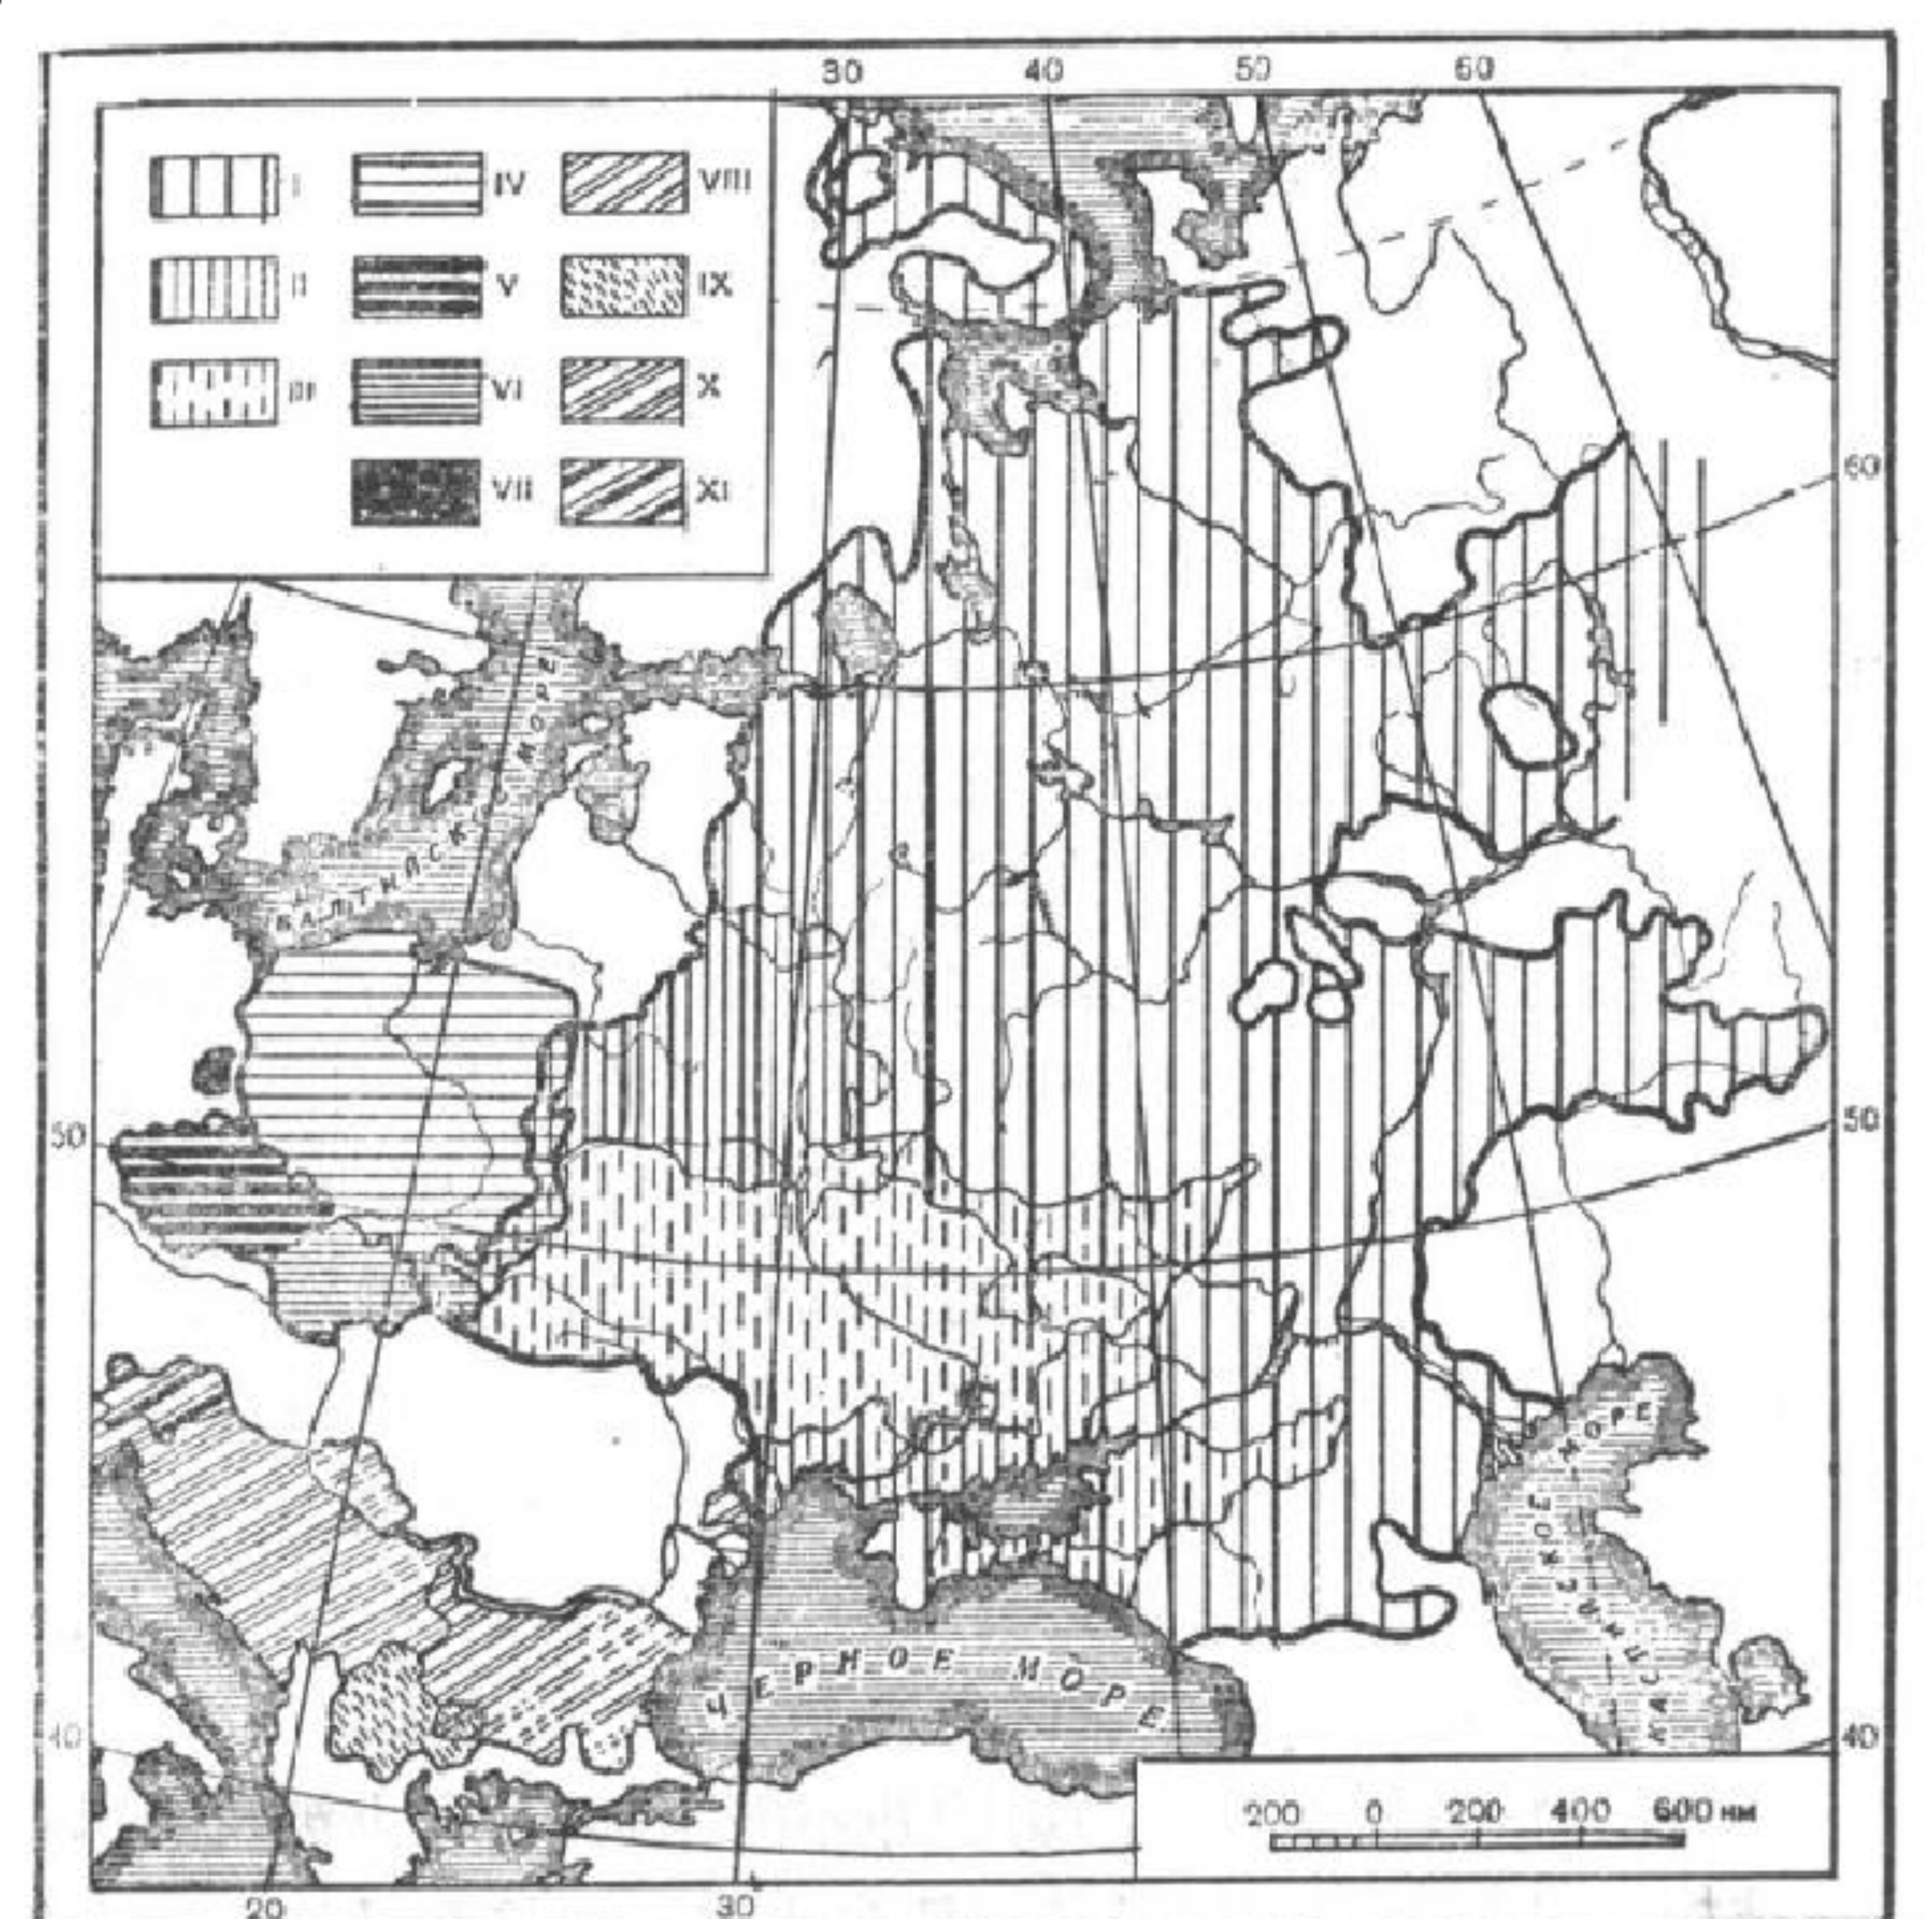
\includegraphics[width=0.78\textwidth]{slavic_map_maponly.png}

{\bfseries\sffamily\color{BellaDeep}斯拉夫语分布示意图}\par
\vspace{1.2mm}
\begin{minipage}{0.92\textwidth}\small
\textbf{图例：}I. 俄语；II. 白俄罗斯语；III. 乌克兰语；IV. 波兰语；V. 捷克语；VI. 斯洛伐克语；VII. 索布语；VIII. 保加利亚语；IX. 马其顿语；X. 塞尔维亚--克罗地亚语；XI. 斯洛文尼亚语。\footnote{引自 \term{Бернштейн С. Б. Очерк сравнительной грамматики славянских языков. Москва, 1961, с. 39.}}
\end{minipage}
\end{center}
\end{samepage}
\clearpage

\origitem{0.6}
在漫长的历史发展过程中，斯拉夫人同许多异族（波罗的人、


\sourcepage{8}{26}
日耳曼人、突厥人、凯尔特人、伊朗人等）发生过政治、军事、宗教、文化等方面的接触，有的甚至同化了后者，或被后者所同化。这些接触在斯拉夫语和有关的异族语言中留下了一定的痕迹。

阿瓦尔汗国（6--8 世纪）的统治，在捷克、斯洛伐克、塞尔维亚--克罗地亚、斯洛文尼亚、乌克兰诸语言中留下了一部分突厥语词。东进的斯拉夫人同化了一部分波罗的人以及其他异族。南下的斯拉夫人定居巴尔干半岛后同化了色雷斯人、操突厥语的古保加尔人，后来甚至自称保加利亚人。西迁的斯拉夫人在公元初同化了当地的异族维内特人，至 2 世纪日耳曼人、芬兰人开始接触斯拉夫人时，就称他们为维内特人了，虽然斯拉夫人从未以此自称。定居于捷克、摩拉维亚和波希米亚的斯拉夫人，至公元 5 世纪同化了当地的凯尔特人（瓦拉几亚人），但后者的语言在捷克语中留下了某些痕迹。\footnote{校勘：括号中的“瓦拉几亚人”有误。瓦拉几亚人（Vlachs）通常指东南欧的罗曼语族群体，并非凯尔特人；把波希米亚、摩拉维亚的古代凯尔特居民称为“瓦拉几亚人”是不同族群名称的混淆。}

另一方面，斯拉夫人被异族同化者也不乏其例。定居易北河（斯拉夫人称为“拉巴河”）流域的西斯拉夫人到中世纪时被日耳曼人同化。17--18 世纪时，还曾有人记录这种波拉巴语，编纂词典，但波拉巴语终于消亡了。在南部斯拉夫人中，斯洛文尼亚人的祖先，曾有一部分分别为匈牙利人、罗曼人、日耳曼人所同化。匈牙利语至今仍有许多斯拉夫借词。一部分定居于巴尔干半岛的南部斯拉夫人被希腊人、阿尔巴尼亚人所同化；而另一部分，定居达契亚的，则被后来的摩尔多瓦人、瓦拉几亚人所同化，不过在罗马尼亚语中留下了许多斯拉夫语成分。

应该指出，语言接触留下的影响并不限于词汇，它也涉及到语音甚至语法结构，保加利亚语和马其顿语失去名词变格和动词不定式便是典型的例子。

\origitem{0.7}
斯拉夫语族在印欧语系中的地位有两点值得单独谈一谈。一个是它属于“s 类语言”，另一个是它同波罗的语族的密切关系。

自 19 世纪以来，语言学家就根据古代腭化后舌音 *\term{k′}, *\term{g′}, *\term{g′h} 的演变结果，将印欧诸语言分为两支：“k 类语言”（\term{centum languages; «кентум» языки}）和“s 类语言”（\term{satəm languages; «сатэм» языки}）。\footnote{校勘：\term{centum--satem} 现在通常被看作一组重要的语音同言线，而不是印欧语系最基本的两大谱系分支。吐火罗语属于 \term{centum} 型而地理位置偏东，已足以说明该划分不能直接等同于印欧语的早期二叉分化。}


\sourcepage{9}{27}
属于“k 类”的有希腊语、拉丁语、意大利诸语言、罗曼诸语言、日耳曼诸语言、凯尔特诸语言、吐火罗语、（楔形文字）赫梯语。在这些语言中，原始印欧语的腭化后舌音演变为后舌音。属于“s 类”的有印度--伊朗诸语言、斯拉夫诸语言、波罗的诸语言、亚美尼亚语、阿尔巴尼亚语。在这些语言中，古腭化后舌音演变为前舌擦音（嘶音或嘘音）。这两类语言习惯上以“百”字的拉丁语 \term{centum}（\term{c} 本来读 \term{k}）和阿吠斯陀语\footnote{阿吠斯陀语是《阿吠斯陀》（\term{Avesta} ‘袄教圣经汇编’）所使用的一种中古波斯语，属伊朗语支，已消亡。\par\textbf{校勘：}“中古波斯语”有误。阿吠斯陀语是古伊朗语（\term{Old Iranian}）之一，与古波斯语同属伊朗语支的早期语言，但并非波斯语的中古阶段。中古波斯语特指萨珊时期及其后的 \term{Middle Persian/Pahlavi}。} \term{satəm} 为代表来区别。比较：拉 \term{centum}（百）-- 俄、保、塞 \term{сто}，捷、波 \term{sto}；拉 \term{decem}（十）-- 俄 \term{десять}，保、塞 \term{десет}，捷 \term{deset}，波 \term{dziesięć}；拉 \term{cor}（心）（属格 \term{cordis}）-- 俄 \term{сердце}，保 \term{сърце}，塞 \term{срце}，捷 \term{srdce}，波 \term{serce}；拉 \term{grānum}（谷物）-- 俄 \term{зерно}，保 \term{зърно}，塞、捷 \term{zrno}，波 \term{ziarno}。（参看 1.2.5）

\origitem{0.8}
在印欧语系中，斯拉夫语族同波罗的语族（立陶宛语、拉脱维亚语和古普鲁士语）关系最近。这两个语族在语音、语法和词汇方面有许多引人注意的共同特征。拿基本词汇来说，有许多共同词或对应词是其他印欧语所无的：斯拉夫语 \term{noga} ‘脚，腿’（俄 \term{нога}，捷 \term{noha}），立 \term{nagà}（蹄），拉脱 \term{nags}（爪），普 \term{nagutis}（爪），比较：拉 \term{pēs}〔法 \term{pied}〕，哥 \term{fotus}〔德 \term{Fuß}，英 \term{foot}〕；斯拉夫语 \term{rǫka} ‘手，臂’（俄 \term{рука}，捷 \term{ruka}，波 \term{ręka}），立 \term{rankà}，比较：拉 \term{manus}〔法 \term{main}〕，哥 \term{handus}〔德 \term{Hand}，英 \term{hand}〕；斯拉夫语 \term{golva} ‘头’（俄 \term{голова}，捷 \term{hlava}，波 \term{głowa}），立 \term{galvà}，拉脱 \term{galvà}，普 \term{galwo}，比较：拉 \term{caput}〔德 \term{Haupt}，英 \term{head}，法 \term{tête}〕。

有些语言学家，如施莱谢尔（\term{A. Schleicher}）、勃鲁格曼（\term{K. Brugmann}）、沙赫玛托夫（\term{А. А. Шахматов}）、波热津斯基（\term{V. K. Porzeziński}）、罗兹瓦多夫斯基（\term{J. Rozwadowski}）、胡耶尔（\term{O. Hujer}）、瓦扬（\term{A. Vaillant}）、格奥尔基耶夫（\term{В. Георгиев}），认为在原始印欧语解体后，存在过一段波罗的--斯拉夫母语时期，后来（约在公元前 1 千纪中叶）才分化为原始波罗的语和原始斯拉夫语。但这个观点遭到许多


\sourcepage{10}{28}
学者的批驳，如博杜恩·德·库尔德内（\term{И. А. Бодуэн де Куртенэ}）、梅耶（\term{A. Meillet}）、恩泽林（\term{J. Endzelin}）、伊利因斯基（\term{Г. А. Ильинский}）、菲林（\term{Ф. П. Филин}）、贝恩施坦（\term{С. Б. Бернштейн}），都认为从未有过波罗的--斯拉夫母语，两个语族之间许多共同或相似的特征无法追溯至同一个来源，而是较晚时期平行发展过程中产生的，因为波罗的人与斯拉夫人长期毗邻而居，交往频繁。\footnote{今按：20 世纪这一争论后来出现了明显的学术重心变化。现代印欧比较语言学通常承认一个可重建的原始波罗的--斯拉夫阶段（\term{Proto-Balto-Slavic}），依据包括共同的音系、形态和重音创新；仍有争议的主要是内部支化方式、接触层次与年代，而不是“是否存在任何共同祖语”本身。}后一派反对使用“波罗的--斯拉夫母语”这个术语，但其中有些人主张采用“共同语”（\term{Einheit; единство}）、“共通语”（\term{Gemeinschaft; общность}）或“互通语”（\term{Verkehrsgemeinschaft; сообщность}），以此来强调共同性并不是（至少不都是）可以重拟的同源现象，而是在两个民族长期接触、平行发展过程中互相交流的产物。

\origitem{0.9}
斯拉夫文字产生于 9 世纪下半叶，那是拜占廷传教士基里尔（\term{Kyrillos}）和美多迪（\term{Methodios}）以希腊字母为基础，根据马其顿方言创制的。现代的斯拉夫字母（所谓基里尔字母）便由此演变而来。\footnote{校勘：这里把“最初的斯拉夫文字”和“基里尔字母”混为一体。现代研究通常认为君士坦丁--基里尔在摩拉维亚传教前创制的是格拉哥里字母（\term{Glagolitic}）；基里尔字母稍后在保加利亚、尤其普雷斯拉夫文字中心形成，以希腊安色尔体为主要基础，并吸收若干表示斯拉夫语特有音的符号。原书第二章 2.2.1 实际也采取了这一较准确的区分。}9 世纪的原本没有流传下来，现存最古的斯拉夫文献是 10 世纪的，如《多布罗加碑文》（943 年）、《萨穆伊勒王碑文》（993 年）、《基辅残篇》（又称《基辅弥撒曲集》，10 世纪）。（详见 2.1.1--2.1.4）

然而，由于历史、宗教、文化影响等原因，并非所有的现代斯拉夫人都使用基里尔字母。如今，使用这种字母的只有东斯拉夫人和南部斯拉夫人中的保加利亚人、马其顿人和塞尔维亚人；西斯拉夫人和南部斯拉夫人中的克罗地亚人、斯洛文尼亚人则使用拉丁字母。

\origitem{0.10}
现代斯拉夫人所使用的基里尔字母（又称斯拉夫字母）同古代的相比有两方面的不同。一是笔划经过简化便于书写了。二是为了适应不同语言的需要，字母有所增减。增加的字母，一部分是由基里尔字母改制而成的，如俄语的 \term{ё}，白俄罗斯语的 \term{ў}，塞尔维亚语和马其顿语的 \term{љ, њ, џ}，马其顿语的 \term{ѓ, ќ} 等；另一部分是借自拉丁语或者由拉丁字母改制而成的，如乌克兰语的 \term{і, ї}，塞尔维亚语和马其顿语的 \term{ј}，塞尔维亚语的 \term{ћ, ђ}。因此，确切地说，基里尔字母只是这些文字的基础。


\sourcepage{11}{29}
表 1 所列的字母中包括经过改革的基里尔字母和借自拉丁语的字母。“基本读音”栏中未加说明者是通用的，凡只为少数语言采用的都作了限定性的说明。所注的音标都是该字母的主要表音功能，不包括实际拼读中各种可能的变化，如浊音字母在词末读作清音等等。

\subsection*{表 1　现代斯拉夫（基里尔）字母一览表}
\small
\begin{longtable}{>{\LingFont}p{0.08\textwidth} p{0.49\textwidth} >{\LingFont}p{0.25\textwidth}}
\toprule
\textbf{斯拉夫字母} & \textbf{基本读音} & \textbf{相应的拉丁字母}\\
\midrule\endfirsthead
\toprule\textbf{斯拉夫字母} & \textbf{基本读音} & \textbf{相应的拉丁字母}\\\midrule\endhead
а & [a] & a\\
б & [b] & b\\
в & [v]；乌：[w] = [u̯] & v；w\\
г & [g]；乌、白：[ɦ], [ɣ] & g；捷：h\\
ѓ & 马：[d′] = [dž′] & 克：đ\\
д & [d] & d\\
ђ & 塞：[d′] = [dž′] & 克：đ\\
е & 俄、白：[′e], [je]；乌、保、塞、马：[e] & e\\
ё & 俄、白：[′o], [jo] & jo\\
є & 乌：[′e], [je] & je\\
ж & [ž] = [ʒ] & ž；波：ż\\
з & [z] & z\\
ѕ & 马：[dz] & dz\\
и & [i]；乌：[ɪ] & i；y\\
й & [j] 或 [ij] & j\\
і & 乌、白：[i] & i\\
ї & 乌：[ji] & ji\\
ј & 马、塞：[j] 或 [i] & j\\
к & [k] & k\\
ќ & 马：[ḱ]（接近 [tś′]） & ć\\
л & [l], [ɫ], [l′] & l\\
љ & 马、塞：[l′]（接近 [ʎ]） & lj\\
м & [m] & m\\
н & [n] & n\\
њ & [n′]（接近 [ɲ]） & nj\\
о & [o] & o\\
п & [p] & p\\
р & [r]（舌尖颤音） & r\\
с & [s] & s\\
т & [t] & t\\
ћ & 塞：[ć]（接近 [tś′]） & ć\\
у & [u] & u\\
ў & 白：[u̯] = [w] & w\\
ф & [f] & f\\
х & [ch] = [x] & ch\\
ц & [c] = [ts] & c\\
ч & [č] = [tš] & č\\
џ & 塞、马：[dž] = [dʒ] & 克：dž\\
ш & [š] = [ʃ] & š\\
щ & 俄：[š′:] 或 [š′č′]；乌：[šč]；保：[št] & šč；šč；št\\
ъ & 保：[ə]；俄：分音符 & --\\
ы & 俄、白：[y] = [ɨ] & 波：y\\
ь & 软音符号；分音符 & --\\
э & 俄、白：[e] & e\\
ю & [′u], [ju] & ju\\
я & [′a], [ja] & ja\\
\bottomrule
\end{longtable}
\normalsize

\origitem{0.11}
\sourcepage{12}{30}
现代斯拉夫人所使用的拉丁字母中，也有一部分是为了适应


各自需要而加以改造的：利用附加符号，如捷克语的 \term{á, ů, č, š, ž, ř}，波兰语的 \term{ą, ę, ć, ś, ź, ż, ł}；利用字母组合，如波兰语的 \term{cz, sz, rz}，捷克语、斯洛伐克语、波兰语的 \term{ch}，克罗地亚语的 \term{lj, nj}。严格说来，这些文字只是以拉丁字母为基础而形成的。

\subsection*{表 2　现代斯拉夫语使用的拉丁字母一览表}
\small
\begin{longtable}{>{\LingFont}p{0.08\textwidth} p{0.49\textwidth} >{\LingFont}p{0.25\textwidth}}
\toprule
\textbf{拉丁字母} & \textbf{基本读音} & \textbf{相应的斯拉夫字母}\\
\midrule\endfirsthead
\toprule\textbf{拉丁字母} & \textbf{基本读音} & \textbf{相应的斯拉夫字母}\\\midrule\endhead
 a & [a] & а\\
 á & 捷、斯伐：[a:] & а\\
 ą & 波：[ǫ] = [õ] & （古斯 ѫ）\\
 ä & 斯伐：[ɛ] 或 [æ] & （古斯 ѧ）\\
 b & [b] & б\\
 c & [c] = [ts] & ц\\
 č & [č] = [tš], [tʃ] & ч\\
 ć & 波、克、高索：[tɕ] = [ć] & 塞：ћ\\
 cz & 波：[č] & ч\\
 d & [d] & д\\
 ď & 捷、斯伐：[d′] & д(ь)\\
 đ & 克：[dž′] & 塞：ђ；дж(ь)\\
 dz & 斯伐：[dz] & дз\\
 dž & 斯伐、克、低索：[dž] & дж；塞：џ\\
 dź & 波、高索：[dʑ] = [dž′] & дж(ь)；塞：ђ\\
 dż & 波：[dž] = [dʒ] & дж\\
 e & [e]；斯文：[e] 和 [ə] & э, е\\
 é & 捷、斯伐：[e:] & э, е\\
 ě & 捷：[je], [′e]；高索：[ie] & （古斯 ѣ）\\
 ê & 斯文：[ei] & --\\
 ę & 波：[ę] = [ẽ] & （古斯 ѧ）\\
 f & [f] & ф\\
 g & [g] & г\\
 h & 捷、斯伐、高索：[ɦ]；波、斯文、克：[ch] = [x] & 乌：г；х\\
 ch & 捷、斯伐、波、高索：[ch] = [x] & х\\
 i & [i] & и\\
 í & [i:] & и\\
 j & [j] 或 [i] & й\\
 k & [k] & к\\
 l & [l] & л\\
 ł & 波：[w] 或 [ɫ]；高索：[w] & л(ъ)；白：ў\\
 ľ & 斯伐：[l′] & л(ь)\\
 ĺ & 斯伐：[l:] & л\\
 lj & 斯文、克：[l′] & л(ь)；塞、马：љ\\
 m & [m] & м\\
 n & [n] & н\\
 ň & 捷、斯伐：[n′] & н(ь)\\
 ń & 波、高索：[n′] & н(ь)\\
 nj & 克、斯文：[n′] & н(ь)；塞、马：њ\\
 o & [o] & о\\
 ó & 捷、斯伐：[o:]；波：[u]；高索：[o]（闭） & о；у\\
 ô & 斯伐、斯文：[uo] & --\\
 ou & 捷：[ou] & --\\
 p & [p] & п\\
 qu & [kv] & кв\\
 r & [r]（舌尖颤音） & р\\
 ř & 捷：[ř] = [rž]；高索：[š] = [ʃ] & рж, р(ь)；ш\\
 ŕ & 斯伐：[r:] & р\\
\sourcepage{13}{31}
 rz & 波：[ž] = [ʒ] & ж\\
 s & [s] & с\\
 š & [š] = [ʃ] & ш\\
 ś & 波：[ɕ] 或 [ś] & ш(ь)\\
 sz & 波：[š] = [ʃ] & ш\\
 t & [t] & т\\
 ť & 捷、斯伐：[t′] & т(ь)\\
 u & [u] & у\\
 ú & 捷、斯伐：[u:] & у\\
 ů & 捷：[u:] & у\\
 v & [v] & в\\
 w & 波、斯伐：[v]；高索：[w] & в；白：ў\\
 x & [ks], [gz] & кс, гз\\
 y & 波、高索：[y] = [ɨ]；捷、斯伐：[i] & 俄：ы；и\\
 ý & 捷：[i:] & и\\
 z & [z] & з\\
 ž & [ž] = [ʒ] & ж\\
 ż & 波：[ž] = [ʒ] & ж\\
 ź & 波：[ź] = [ž′] & ж(ь)\\
\bottomrule
\end{longtable}
\normalsize


\origitem{0.12}
本书标音时尽量采用斯拉夫语言学界习用的拉丁字母。这套符号跟国际音标基本上一致，不同之处主要是：

\begin{center}
\begin{tabular}{>{\LingFont}c >{\LingFont}c l}
\toprule
\textbf{本书音标} & \textbf{国际音标（必要时使用）} & \textbf{说明}\\
\midrule
ǫ & õ & 鼻化的 o\\
ę & ẽ & 鼻化的 e\\
y & ɨ & 央高元音，俄语的 ы\\
ch & x & 后舌清擦音\\
š & ʃ & 前舌清擦音，嘘音\\
ž & ʒ & 前舌浊擦音，嘘音\\
c & ts & 前舌清塞擦音\\
č & tʃ & 前舌清塞擦音，嘘音\\
\bottomrule
\end{tabular}
\end{center}

腭化音即软音用“′”表示；必要时可用国际音标表示，例如：\term{n′ = ɲ, l′ = ʎ, r′ = rʲ}。

\sourcepage{14}{32}
成节功能用“°”表示；必要时可用国际音标的成节符号表示，例如：\term{l° = l̩, r° = r̩}。



\chaptercoverpage{第一章}{原始斯拉夫语（语音）}{ch01.jpg}
\chapter{原始斯拉夫语（语音）}

\origitem{1.0}
原始斯拉夫语从原始印欧语中分化出来以后，大概存在了几千年。它的发展过程可以大致分为前后两个时期。前期包括波罗的--斯拉夫互通语及其分化后的阶段。在这个时期，原始斯拉夫语是统一的，没有明显的方言分歧，从原始印欧语继承下来的闭音节也没发生什么变化。后期始自公元前 3--2 世纪。这一时期的主要变化是由于开音节规律的作用，原来的闭音节以各种方式被排除，致使语音结构乃至形态系统发生深刻变化，同时方言差别渐渐加深，终于在公元 6 世纪左右分化为东、南、西三支不同的斯拉夫语。

本章要讲的是原始斯拉夫语的语音结构，包括元音、辅音的组成和来源（同原始印欧语的继承关系）以及主要的语音变化。

\section*{1. 元音}
\phantomsection\addcontentsline{toc}{section}{1. 元音}
\origitem{1.1.1}
原始斯拉夫语初期的元音、带元音的音组以及成节辅音\footnote{传统讲法多把这几种音和音组并为元音类。}有：

\begin{center}
\begin{tabular}{>{\bfseries}l >{\LingFont}l}
单元音： & a, o, ě, e, u, i, y, ъ, ь;\\
二合元音： & e, o + i̯, u̯（1.3.5）;\\
双元音组合： & e, o, a + n, m, l, r（1.3.6--1.3.8）;\\
成节流音： & l°, r°（1.3.4）。
\end{tabular}
\end{center}


这些元音都从原始印欧语继承下来，而且同其他印欧语中的元音有一定的对应关系。单元音的主要对应关系如下表：

\begin{center}
\sourcepage{15}{33}
\begin{tabularx}{0.99\linewidth}{*{8}{C}}
\toprule
原印 & 原斯 & 古斯 & 梵 & 希 & 拉 & 立 & 日（哥）\\
\midrule
{}*ā & *a & а & ā & ᾱ, η\textsuperscript{1} & ā & ō & --\\
{}*ō & *a & а & ā & ω & ō & uo（旧写法 ū） & ō\\
{}*ă & *o & о & a & α & a & a & a\\
{}*ŏ & *o & о & a & ο & o & a & a\\
{}*ē & *ě & ѣ & ā & η & ē & ė & ē\\
{}*ĕ & *e & е & a & ε & e & e & i, e\\
{}*ū & *y & ы & ū & ῡ & ū & ū & ū\\
{}*ŭ & *ъ & ъ & u & υ & u & u & u\\
{}*ī & *i & и & ī & ῑ & ī & y & i\\
{}*ĭ & *ь & ь & i & ι & i & i & i\\
\bottomrule
\end{tabularx}
\end{center}
\footnotetext[1]{在古希腊语中，ā 一般保留为 ā；只在爱奥尼亚--阿提卡方言中 ā $>$ η [ē]。}

\origitem{1.1.2}
{}*a 来源于原始印欧语的长元音 *ā、*ō，就是说，原来的 ā 和 ō 失去区别，在原始斯拉夫语中合流，成为一个元音。

\noindent\term{*a < *ā:}

原斯 \term{*mati}（母亲），古斯 \term{мати}，梵 \term{mātár-}，希 \term{μήτηρ}（多里安方言 \term{μάτηρ}），拉 \term{māter}，立 \term{móteris}（‘已婚女人’，属格），古德 \term{muoter}〔德 \term{Mutter}，英 \term{mother}〕；

原斯 \term{*bratrъ}（兄，弟），古斯 \term{братръ}，梵 \term{bhrā́tar-}，希 \term{φράτηρ}（族盟的成员），拉 \term{frāter}，哥 \term{brōþar}，古德 \term{bruoder}，撒 \term{brōther}〔德 \term{Bruder}，英 \term{brother}〕。\footnote{本章有些地方引了现代英、德、法语的例词，目的不是直接比较，而是帮助读者建立联想，便于记忆，所以置于方括弧内。}

\noindent\term{*a < *ō:}

\sourcepage{16}{34}
原斯 \term{*duva}（二），古斯 \term{дъва}，梵 \term{dvā}，希（荷马）\term{δύω}，拉 \term{duo}，哥 \term{twai, twos}，古德 \term{zwene, zwo}〔德 \term{zwei}，英 \term{two}〕；


原斯 \term{*darъ}（赠品），\term{*dati}（给），古斯 \term{даръ, дати}，原印 \term{*dō-}，梵 \term{dā́nam}，希 \term{δῶρον}，拉 \term{dōnum}，立 \term{dúoti}。

ā、ō 合流现象也见于其他印欧语。ā、ō 在梵语中并为 ā，在日耳曼语（如哥德语）中并为 ō。但在希腊、拉丁、立陶宛诸语言中演变结果不同。

\origitem{1.1.3}
{}*o 来源于原始印欧语的短元音 *ă、*ŏ，换言之，原来的 ă 和 ŏ 失去区别，在原始斯拉夫语中合流，成为一个元音。

\noindent\term{*o < *ŏ:}

原斯 \term{*domъ}（房屋），古斯 \term{домъ}，梵 \term{dámaḥ}，希 \term{δόμος}，拉 \term{domus}；

原斯 \term{*okos}（眼睛），古斯 \term{око}，梵 \term{ákṣi}，希 \term{ὄσσε}（$<$ \term{*okʷie}），拉 \term{oculus}；

原斯 \term{*ovьka}（绵羊），古斯 \term{овьца}，梵 \term{avikā́}，希 \term{ὄϊς}，拉 \term{ovis}。

\noindent\term{*o < *ă:}

原斯 \term{*otьcь}（父亲），古斯 \term{отьць}，希 \term{ἄττα}（爸爸），哥 \term{atta}，赫 \term{attas}；

原斯 \term{*sol-}（盐），古斯 \term{соль}，拉 \term{sālsus}，哥 \term{salt}〔德 \term{Salz}，英 \term{salt}〕。

ă、ŏ 合流的现象还见于梵语、立陶宛语、哥特语，都是变为 a，但是希腊语和拉丁语中保持着区别：ă $>$ a，ŏ $>$ o。

\origitem{1.1.4}
{}*ě 主要源于原始印欧语的长元音 ē：

原斯 \term{*sěmen}（种子），古斯 \term{сѣме}，拉 \term{sēmen}，立 \term{sėmens}；

原斯 \term{*zvěrь}（野兽），古斯 \term{звѣрь}，希 \term{θήρ}，立 \term{žvėris}；

原斯 \term{*ěd-ętь}（〔他们〕吃），古斯 \term{ѣдѧтъ (јадетъ)}，梵 \term{ād-i-vān}（过去时主动分词），希 \term{ἐδ-ηδ-ώς}（意同梵），拉 \term{ēd-imus}（〔我们〕吃），赫 \term{et-mi}（〔我〕吃）。

{}*ě 的另一个来源是二合元音 \term{oi}，如 \term{*cěna}（代价）$<$ \term{*kʷoinā}。不过，这个变化发生在较晚时期（详见 1.3.5）。

这个元音有两种表示法：或用捷克字母 \term{ě}，或用古斯拉夫字母 \term{ѣ}


\sourcepage{17}{35}
（名称 \term{ять}）。\footnote{为了减少排版技术上的困难，本书一般用 \term{ě}。}关于它的音值学术界看法不一：有人认为 *ě 是单元音，有人认为是二合元音；认为是单元音的人，有的说音值介于 e-a 之间，有的说介于 e-i 之间。考虑到 *ě 后来在各斯拉夫语中的演变结果不同（1.6.1），许多学者推断，原始斯拉夫语中 *ě 的发音在不同时期、不同地域可能是不尽相同的。

\origitem{1.1.5}
{}*e 源于原始印欧语的短元音 *ĕ：

原斯 \term{*nebos}（天空），古斯 \term{небо}，梵 \term{nábhaḥ}（天空，云），希 \term{νέφος}（云），拉 \term{nēbŭla}（云，雾），古德 \term{nebul}（云，雾）〔德 \term{Nebel}（雾，烟雾）〕；

原斯 \term{*desętь}（十），古斯 \term{десѧть}，梵 \term{daśát}，希 \term{δέκα}，拉 \term{decem}，立 \term{dešimt}；

原斯 \term{*berǫ}（〔我〕拿，采摘），古斯 \term{берѫ}，梵 \term{bhárāmi}，希 \term{φέρω}，拉 \term{ferō}，立 \term{beriù}（$<$ \term{bherō}）。

\origitem{1.1.6}
{}*y（古斯 \term{ы}）是由原始印欧语的长元音 *ū 失去唇化特征后演变而成的：

原斯 \term{*ty}（你），古斯 \term{ты}，希（多里安方言）\term{τυ}，拉 \term{tū}〔法 \term{tu}〕，立 \term{tù}，古德 \term{dū, du}〔德 \term{du}〕；

原斯 \term{*synъ}（儿子），古斯 \term{сынъ}，梵 \term{sūnúḥ}，立 \term{sūnùs}，哥 \term{sunus}〔德 \term{Sohn}，英 \term{son}〕；

原斯 \term{*myšь}（鼠），古斯 \term{мышь}，梵 \term{mū́ḥ}，希 \term{μῦς}，拉 \term{mūs}，古德 \term{mūs}〔德 \term{Maus}，英 \term{mouse}〕。

此外，词末尾的 -y 在原始斯拉夫语时期还可能源于 \term{-uns, -ons, -ans}（详见 1.3.6 之 3）。

\sourcepage{18}{36}
这个音也有两个表示法：捷克字母 \term{y}\footnote{\term{y} 在现代捷克语中的读音已和 \term{i} 相同，但在波兰语、索布语中仍与 \term{i} 不同。}；古斯拉夫字母 \term{ы}。关于它在原始斯拉夫语中的音值，学术界意见不一。少数人认为是二合元音，多数人认为是单元音，虽然承认它在不同时期和地域的发音可能有差别（特别是起音和收音阶段）。它在现代俄语中作为一个特殊的央高元


音保留下来，尽管不少学者不承认它是独立的音位。

\origitem{1.1.7}
{}*i 主要来源于原始印欧语的长元音 *ī：

原斯 \term{*piti}（喝），古斯 \term{пити}，梵 \term{pītiḥ}，希 \term{πῖθι}（命令式）；

原斯 \term{*živъ}（$<$ \term{*givъ} ‘活着的’），古斯 \term{живъ}，梵 \term{jīváḥ}，拉 \term{vīvus}（$<$ \term{*gʷīuos}）〔法 \term{vif, vive}〕，立 \term{gývas}；

原斯 \term{*svin-}（猪），古斯 \term{свинија}，拉 \term{suīnus}（猪的），哥 \term{swein}，古德 \term{swīn}〔德 \term{Schwein}，\term{ei < ī}〕。

此外，*i 还源于二合元音 \term{*ei, *oi}，如 \term{*zima}（冬天）$<$ \term{*g'hei-}。不过，这一变化发生在较晚时期（详见 1.3.5）。

\origitem{1.1.8}
{}*ъ、*ь 分别源于原始印欧语的短元音 *ŭ、*ĭ。

\noindent\term{*ъ < *ŭ:}

原斯 \term{*dъkti}（$<$ \term{*dŭkti} ‘女儿’），古斯 \term{дъшти}，梵 \term{duhitár-}，希 \term{θυγάτηρ}，立 \term{duktė}，哥 \term{dauhter}〔英 \term{daughter}，德 \term{Tochter}〕；

原斯 \term{*snъcha}（$<$ \term{*snŭsa} ‘儿媳’），古斯 \term{снъха}，梵 \term{snuṣā́}，希 \term{νυός}（$<$ \term{*snusos}），拉 \term{nūrus}（$<$ \term{*snusos}），古德 \term{snur}（$<$ \term{*snūs-}）；

原斯 \term{*mъchъ}（苔藓），古斯 \term{мъхъ}，拉 \term{mūscus}，立 \term{mūsos}，古德、撒 \term{mos}。

\noindent\term{*ь < *ĭ:}

原斯 \term{*ovьca}（$<$ \term{*ovĭka} ‘绵羊’），古斯 \term{овьца}，梵 \term{avikā́}，希 \term{ὄϊς}，拉 \term{ovis}，立 \term{avis}；

原斯 \term{*vьdova}（$<$ \term{*vĭdovā} ‘寡妇’），古斯 \term{вьдова}，梵 \term{vidhávā}，拉 \term{vidua}，哥 \term{widuwō}，普 \term{widdewū}〔英 \term{widow}，德 \term{Witwe}〕。

{}*ъ 是后元音，音值可能介于 u-y（ы）之间，也许接近现代保加利亚语中的 \term{ъ}（国际音标 [ə]）。*ь 是前元音，音值大概介于 i-e 之间，与国际音标的 [ɪ] 相近。这两个元音特别短，比一般的短元音还要短，而且很可能舌位不大固定，音值不甚清晰，因为它们是 *ŭ、*ĭ 发音缩短、减弱、变开（舌位降低）而形成的（*ŭ $>$ *ъ 还经历了非唇化的过程）。

为了强调这两个音的特殊性，学术界一向用专门的术语来称它们，


\sourcepage{19}{37}
但术语却很不统一：无理元音（\term{иррациональные}），半元音（\term{полугласные}），清元音（\term{глухие}），弱化元音（\term{редуцированные}），特短元音（\term{сверхкраткие}），耳语元音（\term{шёпотные}）。这些术语大都不太理想。“无理元音”（福尔图纳托夫借自数学术语“无理数”）含义不明确，现已无人使用。“半元音”现在习指不能构成音节核心的元音成分，如 \term{i̯, u̯} 等，而 *ъ、*ь 都能构成音节：\term{*mъ-chъ}（苔藓），\term{*dь-nь}（天，日）。“清元音”的缺点在于清浊是就带不带嗓音而言的，而 *ъ、*ь 是带嗓音的元音；当然叫作“耳语元音”也不妥，因为耳语时声带不振动。“弱化元音”目前用得最广，但也不确切，因为弱化元音现在通常用来指非重读音节中发音动作减弱的元音，而 *ъ、*ь 是可以带重音的。相比之下，“特短元音”较为可取，但它忽视了“弱”的特点。本书下文以“短弱元音”称之。



\section*{2. 辅音}
\phantomsection\addcontentsline{toc}{section}{2. 辅音}
\origitem{1.2.1}
原始斯拉夫语最初的辅音有：

\begin{center}
\begin{tabular}{>{\LingFont}l}
p, b, t, d, k, g;\\
s, z, ch, v;\\
j;\\
m, n, l, r.
\end{tabular}
\end{center}

这些辅音是从原始印欧语继承下来的，并同其他印欧语中的辅音有一定的对应关系。一部分比较简单的对应关系如下表：

\begin{center}
\begin{tabularx}{0.99\linewidth}{*{8}{C}}
\toprule
原印 & 原斯 & 古斯 & 梵 & 希 & 拉 & 立 & 日（哥）\\
\midrule
{}*p & *p & п & p & π & p & p & f\\
{}*ph & *p & п & ph & φ & f & p & f\\
{}*b & *b & б & b & β & b & b & p\\
{}*bh & *b & б & bh & φ & f, b & b & b\\
{}*t & *t & т & t & τ & t & t & th\\
{}*th & *t & т & th & θ & t & t & th\\
{}*d & *d & д & d & δ & d & d & t\\
\sourcepage{20}{38}
{}*dh & *d & д & dh & θ & f, b, d & d & d\\
{}*k & *k & к & k & κ & k & k & h\\
{}*g & *g & г & g & γ & g & g & k\\
{}*gh & *g & г & gh, h & χ & h & g & g\\
{}*k′ & *s & с & ś (= ç) & κ & k & š & h\\
{}*g′ & *z & з & j & γ & g & ž & k\\
{}*g′h & *z & з & h & χ & h, g & ž & g\\
{}*kᵘ & *k & к & k & π, τ & qu & k & hw\\
{}*gᵘ & *g & г & g & β, δ & v, gv & g & q = kw\\
{}*gᵘh & *g & г & gh, h & φ, θ & v, gv, f & g & w, gw\\
{}*s & *s, *ch & с, х & s, ṣ & σ(ς) & s, r & s, š & s\\
{}*m & *m & м & m & μ, ν & m & m & m\\
{}*n & *n & н & n & ν & n & n & n\\
{}*l & *l & л & r, l & λ & l & l & l\\
{}*r & *r & р & r & ρ & r & r & r\\
\bottomrule
\end{tabularx}
\end{center}


\origitem{1.2.2}
双唇音 \term{*p} 来源于原始印欧语中不送气的 \term{*p} 和送气的 \term{*ph}，\term{*b} 来源于不送气的 \term{*b} 和送气的 \term{*bh}。

\noindent\term{*p < *p, *ph:}

原斯 \term{*sъpati}（$<$ \term{*suep-} ‘睡觉’），古斯 \term{съпати}，梵 \term{svápiti}（〔他〕睡），希 \term{ὕπνος}，拉 \term{sopor}，立 \term{sãpnas}〔古英 \term{swefan}〕；

原斯 \term{*pěna}（$<$ \term{*sphoinā} ‘泡沫’），古斯 \term{пѣна}，梵 \term{phénaḥ}，立 \term{spáinė}，普 \term{spoayno}，古德 \term{feim}〔英 \term{foam}〕。

\noindent\term{*b < *b, *bh:}

原斯 \term{*bratrъ}（兄，弟），古斯 \term{братръ}，梵 \term{bhrā́tar}，希 \term{φράτηρ}（族盟的成员），拉 \term{frāter}〔法 \term{frère}〕，哥 \term{broþar}，古德 \term{bruoder}〔德 \term{Bruder}〕，撒 \term{brōther}〔英 \term{brother}〕；

原斯 \term{*nebos}（天空），古斯 \term{небо}，梵 \term{nábhaḥ}，希 \term{νέφος}（云），拉 \term{nebula}（云，雾），古德 \term{nebul}（云，雾）〔德 \term{Nebel}〕。


\sourcepage{21}{39}
证明 \term{*b < *b} 的实例很少，而且时有争论。人们常举的例子是：

原斯 \term{*bolto}（沼泽），古斯 \term{блато}，立 \term{báltas}（白色的），阿尔巴尼亚 \term{baltë}，古德 \term{pfuol}，英 \term{pool}（水塘）。

\origitem{1.2.3}
\term{*t} 来源于原始印欧语中不送气的 \term{*t} 和送气的 \term{*th}，\term{*d} 来源于不送气的 \term{*d} 和送气的 \term{*dh}。

\noindent\term{*t < *t, *th:}

原斯 \term{*trejes, *trьje}（三），古斯 \term{трије, трьје, три}，梵 \term{tráyaḥ}，希 \term{τρεῖς}，拉 \term{trēs}〔法 \term{trois}〕，立 \term{trỹs}，古德 \term{dri}〔德 \term{drei}，英 \term{three}〕；

原斯 \term{*pętь}（$<$ \term{ponth-} ‘道路’），古斯 \term{пѫть}，梵 \term{pánthāḥ}，拉 \term{pons}（属格 \term{pontis} ‘桥’）〔法 \term{pont}〕，普 \term{pintis}。

\noindent\term{*d < *d, *dh:}

原斯 \term{*domъ}（房屋），古斯 \term{домъ}，梵 \term{dámaḥ}，希 \term{δόμος}，拉 \term{domus}；

\sourcepage{22}{40}
原斯 \term{*dymъ}（$<$ \term{*dhūm-} ‘烟’），古斯 \term{дымъ}，梵 \term{dhūmáḥ}，希 \term{θυμός}，拉 \term{fūmus}〔法 \term{fumée}〕，立 \term{dūmai}，普 \term{dumis}，古德 \term{toum}。

\origitem{1.2.4}
关于送气音不得不简单说明一下，因为原始印欧语中究竟有无送气音一直是个悬案。大致说来，有三种观点。

传统观点认为，古代的塞音，无论清的浊的，都有送气不送气的区别：\term{p, t, k} 与 \term{ph, th, kh} 对立；\term{b, d, g} 与 \term{bh, dh, gh} 对立。但是后来它们在大多数印欧语中合流了，只有梵语把送气不送气的对立系统完整地保留下来。

另一种看法是，浊塞音肯定有过送气不送气的区别，因为除梵语之外，还有一些旁证。譬如古代不送气的 \term{b, d} 在日耳曼语、亚美尼亚语中演变为清音 \term{p, t}；送气的 \term{bh, dh} 在拉丁语和希腊语中转化为特殊的清擦音：拉丁 \term{f}，希腊 \term{φ} 和 \term{θ}。至于清音有无送气的区别尚难断言，因为缺乏足够的例证。

按照第三种意见，如果语言中没有某种无标记项，那就不可能有相应的标记项，换言之，既然没有清的送气音，也就不会有浊的送气音。至于梵语中的送气音，那可能不是从原始印欧语继承的，而是在达罗毗荼语或藏缅语影响下产生的。然而有些语言现象用这种观点解释不通，比如在希腊语、亚美尼亚语中送气与不送气清音的演变结果不同。\footnote{关于送气音问题可参看：Мейе А. \textit{Общеславянский язык}. Москва, 1951, с. 19--22, 110--116；Бернштейн С. Б. \textit{Очерк сравнительной грамматики славянских языков}. Москва, 1961, с. 149--151；Савченко А. Н. \textit{Сравнительная грамматика индоевропейских языков}. Москва, 1974, с. 68--71；Бошкович Р. \textit{Основы сравнительной грамматики славянских языков}. Москва, 1984, с. 94--95；Мартине А. \textit{Принцип экономии в фонетических изменениях}. Москва, 1960, с. 153；Jakobson R. “Typological studies and their contribution to historical comparative linguistics”. In: \textit{Proceedings of the Eighth International Congress of Linguists}. Oslo, 1958, p. 17--25；Гамкрелидзе Т. В., Иванов В. В. \textit{Индоевропейский язык и индоевропейцы}. Тбилиси, 1984, с. 5--80.}


\origitem{1.2.5}
后舌音的情况比较复杂。按照勃鲁格曼（\term{K. Brugmann, 1849--1919}）的观点，原始印欧语中的后舌音分三个系列：普通的（单纯的）后舌音 \term{k, g, gh}；腭化的后舌音 \term{k′, g′, g′h}；唇化的后舌音 \term{kᵘ, gᵘ, gᵘh}。这三套音在各印欧语中的演变有所不同。

在原始斯拉夫语中，\term{*k > *k; *g, *gh > *g; *k′ > *s; *g′, *g′h > *z; *kᵘ > *k; *gᵘ, *gᵘh > *g}。例如：

\noindent\textbf{a) }\term{*k < *k; *g < *g, *gh:}

原斯 \term{*krъvь}（$<$ \term{*krū-} ‘血’），古斯 \term{кръвь}，梵 \term{kraviḥ}（生肉），希 \term{κρέας}（肉），拉丁 \term{cruor}，立 \term{kraũjas}；

原斯 \term{*jьgo}（轭），古斯 \term{иго}，梵 \term{yugám}，希 \term{ζυγόν}，拉 \term{jugum}〔法 \term{joug}〕，哥 \term{juk}〔德 \term{Joch}，英 \term{yoke}〕；

原斯 \term{*bogъ}（$<$ \term{*bhog-} ‘上帝，神’），古斯 \term{богъ}，古波斯 \term{baga-}，梵 \term{bhágaḥ}；

原斯 \term{*gostь}（$<$ \term{*ghostis} ‘客商，客人’），古斯 \term{гость}，拉 \term{hostis}（敌人，外国人），哥 \term{gasts}。

\noindent\textbf{b) }\term{*s < *k′; *z < *g′, *g′h:}

原斯 \term{*sъto}（$<$ \term{*k′m̥ton} ‘百’），古斯 \term{съто}，阿吠斯陀 \term{satəm}，梵 \term{śatám}，立 \term{šimtas}；拉 \term{centum}〔法 \term{cent}〕，希 \term{ἑ-κατόν}，哥 \term{hund}〔德 \term{Hundert}，英 \term{hundred}〕；


\sourcepage{23}{41}
原斯 \term{*znati}（$<$ \term{*g′nō-} ‘知道’），古斯 \term{знати}，阿吠斯陀 \term{paitizānənti}，梵 \term{jānāti}，立 \term{žinóti}；希 \term{γι-γνώ-σκω}（〔我〕认识），拉 \term{co-gnō-scō}，哥 \term{kann}〔德 \term{können, kann} ‘能够’，英 \term{can, know}〕；

原斯 \term{*zьrno}（$<$ \term{*g′rn-} ‘谷粒’），古斯 \term{зрьно}，梵 \term{jirṇáḥ}，立 \term{žirnis}（豌豆）；拉 \term{grānum}〔法 \term{grain}〕，古爱尔兰 \term{grán}，哥 \term{kaúrn}，古德 \term{corn}〔德 \term{Korn}，英 \term{corn}〕；

原斯 \term{*zima}（$<$ \term{*g′heim-} ‘冬季’），古斯 \term{зима}，阿吠斯陀 \term{zimō}，梵 \term{himás}，立 \term{žiemà}；希 \term{χεῖμα}，拉 \term{hiems}。

上文（0.7）说过，由于古腭化的 \term{*k′, *g′, *g′h} 在拉丁等语言中演变为后舌音，而在阿吠斯陀等语言中演变为前舌擦音（嘶音或嘘音），因此通常将前者称为“k 类语言”（以拉丁词 \term{centum} ‘百’为代表），而把后者叫作“s 类语言”（以阿吠斯陀词 \term{satəm} ‘百’为代表）。斯拉夫语属于后者。

\noindent\textbf{c) }\term{*k < *kᵘ; *g < *gᵘ, *gᵘh:}

原斯 \term{*vьlkъ}（$<$ \term{*u̯l̥kᵘos} ‘狼’），古斯 \term{влькъ}，梵 \term{vŕ̥kaḥ}，立 \term{vilkas}，希 \term{λύκος}，拉 \term{lupus}〔法 \term{loup}〕，哥 \term{wulfs}〔德 \term{Wolf}，英 \term{wolf}〕；

原斯 \term{*kъ-to}（谁），古斯 \term{къто}，梵 \term{kaḥ}，希 \term{τίς}，拉 \term{quis}〔法 \term{qui}〕，立 \term{kàs}，哥 \term{hvas}；

原斯 \term{*gov-ęd-o}（$<$ \term{*gᵘous} ‘牛羊’），古斯 \term{говѧдо}〔俄 \term{говядина} ‘牛肉’〕，梵 \term{gáuḥ}，阿吠斯陀 \term{gauš}，拉脱 \term{guovs}；希 \term{βοῦς}，古德 \term{chuo}〔德 \term{Kuh}〕，撒 \term{kō, kuo}〔英 \term{cow}〕；

原斯 \term{*sněgъ}（$<$ \term{*snoigᵘh-} ‘雪’），古斯 \term{снѣгъ}，希 \term{νίφα}（宾格），拉 \term{nivem}（宾格），\term{ninguit}（下雪了）〔法 \term{neige}〕，立 \term{sniegas}，普 \term{snaygis}，哥 \term{snaiws}〔德 \term{Schnee}，英 \term{snow}〕。

综上所述，在“k 类语言”中，一般是普通后舌音与腭化后舌音合流；在“s 类语言”中，则是普通后舌音与唇化后舌音合流。就原始斯拉夫语辅音的来源而言，则是：

\begin{center}
\begin{tabular}{>{\LingFont}l}
{}*k $<$ *k, *kᵘ\\
{}*g $<$ *g, *gᵘ, *gh, *gᵘh\\
{}*s $<$ *k′\\
{}*z $<$ *g′, *g′h
\sourcepage{24}{42}
\end{tabular}
\end{center}

不过，\term{*s, *z} 还有其他来源（1.2.6）。


\origitem{1.2.6}
\term{*s, *z} 一部分源于原始印欧语的腭化后舌音（1.2.5），另一部分则源于原始印欧语的 \term{*s, *z}。

\noindent\term{*s < *s:}

原斯 \term{*synъ}（儿子），古斯 \term{сынъ}，梵 \term{sūnúḥ}，立 \term{sūnùs}，哥 \term{sunus}〔德 \term{Sohn}，英 \term{son}〕；

原斯 \term{*sestra}（姊，妹），古斯 \term{сестра}，拉 \term{soror}〔法 \term{sœur}〕，立 \term{sesuõ}，哥 \term{swistar}〔德 \term{Schwester}（\term{sch < s}），英 \term{sister}〕；

原斯 \term{*sedmь}（$<$ \term{*septm̥} ‘七’），古斯 \term{седмь}，梵 \term{saptá}，希 \term{ἑπτά}，拉 \term{septem}〔法 \term{sept}〕，立 \term{septyni}，哥 \term{sibun}〔德 \term{sieben}，英 \term{seven}〕。

\noindent\term{*z < *z:}

原斯 \term{*gnězdo}（$<$ \term{*ni-zdos}，\term{zd < sd < səd} ‘巢’），古斯 \term{гнѣздо}，梵 \term{nidā́ḥ}，拉 \term{nīdus}（$<$ \term{*nizdus}）〔法 \term{nid}〕，立 \term{lizdas}，古德 \term{nest}〔德 \term{Nest}，英 \term{nest}〕；

原斯 \term{*mozgъ}（脑），古斯 \term{мозгъ}，阿吠斯陀 \term{mazga}（骨髓），普 \term{muzgeno}，立 \term{smãgenys}（$<$ \term{*mazgen-}），古德 \term{marg}（$<$ \term{*mazga}）。

在原始印欧语中，\term{*z} 只见于词内音节中的音组 \term{zb, zd, zg}，所以不是独立的音位，只是 \term{*s} 的随位变体。

\origitem{1.2.7}
后舌音 \term{*ch}（或用古斯拉夫字母标作 \term{х}）来源于原始印欧语中某些条件下的 \term{*s}：在元音 \term{i, u} 或辅音 \term{k, r} 之后，而又不在清塞音 \term{p, t, k} 之前时。这里说的 \term{i, u} 长短都包括在内（\term{ī > i, ū > y; ĭ > ь, ŭ > ъ}；二合元音末尾的 \term{i, u}），它们都符合 \term{*s > *ch} 的条件。例如：

\sourcepage{25}{43}
原斯 \term{*trьchъ}（$<$ \term{*trisu} ‘三’，位格），古斯 \term{трьхъ}，希 \term{τρισί}（与格），立 \term{trisù}；


原斯 \term{*mъchъ}（$<$ \term{*mus-} ‘苔藓’），古斯 \term{мъхъ}，拉 \term{muscus}，立 \term{mūsos}，古德 \term{mos}；

原斯 \term{*ucho}（$<$ \term{*au̯s-} ‘耳朵’），古斯 \term{оухо}，拉 \term{auris}（$<$ \term{*ausis}），立 \term{ausìs}，哥 \term{ausō}；

原斯 \term{*vьrchъ}（$<$ \term{*urs-} ‘顶，上面’），古斯 \term{врьхъ}，梵 \term{varṣimā}，拉 \term{verrūca}（$<$ \term{*versuca}），立 \term{viršùs}，拉脱 \term{virsūs}；

原斯 \term{*rěchъ}（$<$ \term{*rēchon < *rēk-s-on} ‘〔我〕说过’，不定过去时），古斯 \term{рѣхъ}（参看 2.4.23）。

如果后面有 \term{p, t, k}，则 \term{s} 保持不变：\term{istina}（真理），\term{iskati}（寻找）。

\term{*s > *ch} 有些例外，但都有原因，其中最常见的是后来由于形态类推作用而产生的 \term{ch}。（参看第 113 页脚注 1）

\origitem{1.2.8}
\term{*j, *v} 大致说来源于原始印欧语的 \term{*j (i̯), *w (u̯)}。例如：

\noindent\term{*j < *j (i̯):}

原斯 \term{*junъ}（年轻的），古斯 \term{юнъ}，梵 \term{yúvā}（属格 \term{yūnáḥ}），拉 \term{jūvēnis}（比较级 \term{jūnior}）〔法 \term{jeune}〕，立 \term{jáunas}，拉脱 \term{jauns}，哥 \term{juggs}，古德 \term{iung}〔德 \term{jung}，英 \term{young}〕；

原斯 \term{*jigo}（$<$ \term{*jьgo} ‘轭’），古斯 \term{иго}，梵 \term{yugám}，希 \term{ζυγόν}，拉 \term{jugum}〔法 \term{joug}〕，立 \term{jùngas}，哥 \term{juk}，古德 \term{juh, joh}〔德 \term{Joch}，英 \term{yoke}〕。

\noindent\term{*v < *w (u̯):}

原斯 \term{*novъ}（$<$ \term{*neu̯os} ‘新的’），古斯 \term{новъ}，梵 \term{návaḥ}，希 \term{νέ(F)ος}，拉 \term{nōvus}（$<$ \term{*nouos}）〔法 \term{nouveau}〕，立 \term{naũjas}，普 \term{nawans}，古德 \term{niuwi}〔德 \term{neu}，英 \term{new}〕；

原斯 \term{*vezǫ}（〔我〕运载），古斯 \term{везѫ}，梵 \term{váhati}（〔他〕运载），拉 \term{vehō}（$<$ \term{*uehō}），立 \term{vežù}。

\origitem{1.2.9}
\sourcepage{26}{44}
响音因能否构成音节核心而大致分为两种情况。一种是原来位于元音前或词首的 \term{m, n, l, r}，在原始斯拉夫语初期作为一般辅音保留下来，没有发生什么变化。在这一点上可以认为 \term{*m, *n, *l, *r < *m, *n, *l, *r}。例如：


原斯 \term{*myšь}（鼠），古斯 \term{мышь}，梵 \term{mūḥ}，希 \term{μῦς}，拉 \term{mūs}，古德 \term{mūs}〔德 \term{Maus}，英 \term{mouse}〕；

原斯 \term{*nebos}（天空），古斯 \term{небо}，梵 \term{nábhaḥ}（云，雾），希 \term{νέφος}（云），拉 \term{nēbŭla}（云，雾），古德 \term{nebul}（云，雾）〔德 \term{Nebel}〕；

原斯 \term{*lučь}（光线），古斯 \term{лоучь}，梵 \term{rōcásm}（\term{r < l}），希 \term{λευκός}（白色的），拉 \term{lūcēre}（发光），\term{lūx}（光），哥 \term{liuhaþ}（光）；

原斯 \term{*berǫ}（$<$ \term{*bher-} ‘〔我〕拿，采摘’），古斯 \term{берѫ}，梵 \term{bhárāmi}，希 \term{φέρω}，拉 \term{fĕrō}，立 \term{beriù}。

另一种情况是位于辅音之间的响音具有成节功能，即起元音的作用：\term{m̥, n̥, l̥, r̥}。关于这些成节音，我们将结合它们的演变过程来阐述（见 1.3.4 和 1.3.6）。

\section*{3. 开音节规律}
\phantomsection\addcontentsline{toc}{section}{3. 开音节规律}
\origitem{1.3.1}
在原始斯拉夫语发展后期，语音结构发生了巨大变化，其中涉及范围最广、影响最为深远的有三个：开音节规律、辅音的软化、短弱元音 \term{ъ, ь} 的消亡。这些变化既改变了单词的语音面貌和语言的音位系统，又牵动了形态变化系统。不言而喻，在原始斯拉夫语解体（约 6 世纪）以前的语音变化，在后来的各支斯拉夫语中都有反映，演变结果也相同（不包括后来的变化）。在原始斯拉夫语出现方言分歧及解体之后发生的语音变化，其演变结果在各支斯拉夫语中自然会有一定的区别。

\sourcepage{27}{45}
开音节规律大约发生在公元前最后数世纪至公元 5--6 世纪。其实质是把最初以辅音和非成节元音（\term{i̯, u̯}）结尾的音节逐渐改造为以元音或成节辅音（\term{l̥, r̥} 等）结尾的音节。排除闭音节的具体方式有：词末辅音脱落；辅音组简化为一个音，或者发生同化、异化；改变音节核心；二合元音（\term{-i̯, -u̯}）变为单元音；音组“元音 + 鼻辅音”变为鼻元音或普通元音；音组“元音 + 辅音”发生易位或者在辅音后滋生新的元音等。

下面就来分别叙述因开音节规律而产生的各种语音变化。


\origitem{1.3.2}
在开音节规律起作用以前，大多数词和词形是以辅音结尾的，不过能在词末尾出现的辅音只有五个前舌音：\term{-t, -d, -s, -n, -r}。后来，这些尾辅音在开音节规律支配下先后脱落，使得实词渐渐都以元音结尾了。比如：

\noindent\term{-t:} 原斯 \term{*beri}（$<$ \term{*bheroit} ‘拿’，单 3 人称命令式），古斯 \term{бери}，梵 \term{bháret}，希 \term{φέροι}，哥 \term{bairai}；

\noindent\term{-d:} 原斯 \term{*to}（$<$ \term{*tod} ‘这’），古斯 \term{то}，梵 \term{tát}，拉 \term{istud}（$<$ \term{*istod}），哥 \term{þat-a}；

原斯 \term{*vьlka}（$<$ \term{*vьlk-ōd} ‘狼’，属格），古斯 \term{влька}，梵 \term{vŕ̥kād}（夺格），立 \term{vilko}（\term{*-ōd} 最初是夺格词尾）；

\noindent\term{-s:} 原斯 \term{*synъ}（$<$ \term{*sūnūs} ‘儿子’，主格），古斯 \term{сынъ}，梵 \term{sūnúḥ}，立 \term{sūnùs}，哥 \term{sunus}；

\noindent\term{-n（在 ъ, ь 后时）:} 原斯 \term{*synъ}（$<$ \term{*sūnūn} ‘儿子’，宾格），古斯 \term{сынъ}，梵 \term{sūnúm}，立 \term{sūnų}（$<$ \term{*-un}），普 \term{sunun}；

原斯 \term{*gostь}（$<$ \term{*gostin} ‘客商’，宾格），古斯 \term{гость}，梵 \term{agním}（$<$ \term{*-in}），希 \term{πόλιν}，立 \term{naktį}（$<$ \term{*-in}），普 \term{naktin}；

\noindent\term{-r:} 原斯 \term{*mati}（$<$ \term{*mātēr} ‘母亲’），拉 \term{māter}，希 \term{μήτηρ}，立 \term{mótė}，古德 \term{muoter}〔德 \term{Mutter}，英 \term{mother}〕；

原斯 \term{*dъkti}（$<$ \term{*dhūgətēr} ‘女儿’），古斯 \term{дъшти}，希 \term{θυγάτηρ}，立 \term{duktė}，哥 \term{dauhtar}〔德 \term{Tochter}，英 \term{daughter}〕。

词末 \term{-n} 的脱落只限于在 \term{ъ, ь} 后，关于其他情况参看 1.3.6。

\origitem{1.3.3}
开音节规律对词内部辅音的影响稍有不同。它首先改变了音节的界线，使本来处在闭音节末尾的辅音并入下一音节：\term{*sъp-nos > *sъ-pnos}（睡眠），\term{*dad-mъ > *da-dmъ}（〔我〕给），\term{*plet-ti > *ple-tti}（编织）等等。这样便使原始斯拉夫语中出现了新的音组。


\sourcepage{28}{46}
原始斯拉夫语的词首端和词内部本来是允许一些辅音组存在的，如“\term{s, z +} 其他辅音”、“\term{ch +} 某些响音”、“塞音 + 某些响音”：\term{*sněgъ}（雪），\term{*zvonъ}（钟，铃），\term{*chlěbъ}（粮食），\term{*bratrъ}（兄，弟），\term{*drugъ}（朋友），\term{grobъ}（棺材）等。一般说来，能在词内部出现的音组，必须是也能在词首出现的。比如 \term{*pe-snь}（歌），\term{*ja-zva}（击伤），\term{*do-brъ}（好的），\term{*i-gra}（游玩）中的 \term{sn, zv, br, gr} 之所以能够存在，是因为它们自古以来便可用在词首。这类音组没有受开音节规律的影响。

倘若音节界线移动后产生的音组是新的，即斯拉夫人过去不习惯的，那就要发生简化、同化或异化等音变。一般规律是发生逆行同化，或者前一个塞音弱化直至消失，个别情况下发生顺行同化，失去后一个音。现在分别举例说明。

\noindent\textbf{1) \term{tl, dl}}　这两个音组在东、南两支斯拉夫语中，可能是经过 \term{tl, dl} 的阶段，最后简化为 \term{l}，但在西斯拉夫语中保持不变。例如：

原斯 \term{*pletlъ}（‘编织’，过去时主动形动词），俄 \term{плёл, плела}，保 \term{плел, плела}，塞 \term{plēo}（\term{o < l}），\term{plela}；捷 \term{pletl, pletla}，波 \term{plótł, plotła}；

原斯 \term{*mydlo}（肥皂），俄 \term{мыло}，塞 \term{milo}；捷 \term{mýdlo}，波 \term{mydło}。

\noindent\textbf{2) \term{ps, bs, ts, ds}}　这几个音组失去前面的塞音，简化为 \term{s}。例如：

原斯 \term{*osa}（$<$ \term{*opsa} ‘黄蜂’），拉 \term{vespa}（$<$ \term{*vospa}），立 \term{vapsà}（牛虻），古德 \term{wafsa}〔德 \term{Wespe}，\term{sp < ps}〕；

原斯 \term{grěsъ}（$<$ \term{*grēbson} ‘〔我〕用桨划’，不定过去时），比较 \term{*grěbǫ}（〔我〕划，现在时），立 \term{grėbiu}（〔我〕耙），哥 \term{graban}（挖掘）；

原斯 \term{*dasi}（$<$ \term{*dadsi} ‘〔你〕给’），比较 \term{*dadętь}（〔他们〕给）；

原斯 \term{*kǫsъ}（$<$ \term{*kondsos} ‘一块’），立 \term{kándu}。

又如 \term{tsl, dsl > sl}: \term{*čislo}（$<$ \term{*čitslo} ‘数目’），比较 \term{*čьtǫ}（〔我〕数）。

\noindent\textbf{3) \term{ks, gs}}　这两个音组简化为 \term{kch > ch}。例如：

\sourcepage{29}{47}
原斯 \term{*těchъ < *tēkchon < *tēkson}（‘流’，不定过去时，单 1 人称）；


原斯 \term{*žachъ < *gechъ < *gēkchon < *gēkson < *gegson}（‘点燃，烧’，不定过去时，单 1 人称）。

\noindent\textbf{4) \term{pn, bn, tn, dn}}　这些音组失去前面的塞音，简化为 \term{n}。例如：

原斯 \term{*sъnъ}（$<$ \term{*sъpnos} ‘睡眠，梦’），动词 \term{sъpati}，梵 \term{svápnaḥ}，希 \term{ὕπνος}，立 \term{sãpnas}；

原斯 \term{*dъno}（$<$ \term{*dubno} ‘底’），立 \term{dúgnas}（$<$ \term{*dubnas}），\term{dubùs}（深的），拉脱 \term{dubens}，普 \term{padaubis}（山谷），哥 \term{diups}（深的）〔英 \term{deep}〕；

原斯 \term{*vęnǫti}（$<$ \term{*vędnǫti} ‘枯萎’），古德 \term{swintan}〔德 \term{schwinden} ‘缩小，减少’〕。

\noindent\textbf{5) \term{tm, dm}}　这两个音组失去前面的塞音，简化为 \term{m}。如：

\term{*vrěme}（$<$ \term{*vertmen-} ‘时间’），比较 \term{*vrьtěti sę}（‘转’，词根 \term{vert/vort/vьrt}），梵 \term{vártma}（轨道）；

\term{*damъ}（$<$ \term{*dadmi} ‘〔我〕给’），梵 \term{dádāti}，希 \term{δίδωμι}；

\term{*plemę}（$<$ \term{*pledmen} ‘部落’），比较 \term{*plodъ}（‘果实’，词根 \term{pled/plod}，\term{e:o} 交替）。

数词 \term{*sedmь}（七）、\term{*sedmъ}（第七）中的音组 \term{dm}（$<$ \term{*bdm}）在南、西两支斯拉夫语中保留下来：保 \term{седем, седми}，塞 \term{sèdam, sèdmi}；捷 \term{sedm, sedmý}，波 \term{siedem, siódmy}。但在东斯拉夫语中大都简化为 \term{m} 了：俄 \term{семь, седьмой}，乌 \term{сім, сьомий}，白 \term{сем, сёмы}。

\noindent\textbf{6) \term{bv}}　这个音组失去后面的擦音，简化为 \term{b}。这是唯一的顺行同化的例子。

\term{*oblako}（$<$ \term{*ob-volko} ‘云’）；

\term{*obratiti}（$<$ \term{*ob-vortiti} ‘使变为’）；

\term{*obiti}（$<$ \term{*ob-viti} ‘包上皮’），立 \term{výti}；

\term{*obitati}（$<$ \term{*ob-vitati} ‘居住’）。

\noindent\textbf{7) \term{tt (< tt, dt)}}　两个塞音相遇发生异化，前一个变为擦音：\term{st}。例如：

\sourcepage{30}{48}
\term{*plesti}（$<$ \term{*pletti} ‘编织’），比较 \term{*pletǫ}（〔我〕编织）；


\term{*mesti}（$<$ \term{*metti} ‘扫’），比较 \term{*metǫ}（〔我〕扫），立 \term{mėsti, metù}；

\term{*vesti}（$<$ \term{*vedti} ‘带领’），比较 \term{*vedǫ}（〔我〕带领），立 \term{vèsti, vedù}；

\term{*sěsti}（$<$ \term{*sēdti} ‘坐下’），比较 \term{sędǫ}（〔我〕坐下），立 \term{sėsti, sėdu}，拉 \term{sedeo}（〔我〕坐），哥 \term{sitan}（‘坐’，不定式）。

\noindent\textbf{8) \term{kt}}　在一般情况下是失去前面的塞音，简化为 \term{t}。例如：

\term{*pętь}（$<$ \term{*penkᵘtos} ‘第五’），立 \term{peñktas}；

\term{*potъ}（$<$ \term{*poktos} ‘汗水’），比较 \term{*pekti}（烤）（\term{o:e} 交替）。

\origitem{1.3.4}
这两个成节流音究竟是从原始印欧语继承的，还是后来在波罗的--斯拉夫互通语时期由音组 \term{ur, ir, ul, il} 演变来的，学术界尚无定论。不过学者们大都承认以下两点：

1）原始斯拉夫语时期的成节流音，实际上是音组“半元音成分 + \term{r, l}”，而半元音的舌位又有前后的不同，一说是腭化与后舌化之分：\term{ьr, ъr, ьl, ъl}；

2）这些音组，从实际发音来说，音节核心是流音，所以明确的表示方法应该是 \term{r̥, l̥}。

在这些音组中，流音之所以起元音的作用，是因为开音节规律不允许闭音节存在。于是，\term{*vьlkъ > *vьl̥-kъ}（狼），\term{*vьr-ba > *vьr̥-ba}（柳）。至于流音前半元音成分的舌位前后（腭化、后舌化）之分，那是从后来的演变结果推断出来的。比较：\term{*gъrdlo >} 俄 \term{горло}，波 \term{gardło}（喉）；\term{*gьrdlo >} 俄 \term{жерло}，波 \term{źródło}（深窄的孔，口）。（关于 \term{dl > l} 见 1.3.3 之 1）

后来的演变可大别为两类。

\sourcepage{31}{49}
一类是流音失去成节功能，变成普通的辅音 \term{r, l}，而其前的半元音成分变为音节核心。简言之，变为“成节元音 + 辅音 \term{r, l}”的音组。东斯拉夫语、保加利亚语、波兰语便是如此。


另一类则程度不同地保留着 \term{r̥, l̥} 的成节功能，只是由于半元音成分的消失，腭化与后舌化的区别也不复存在了。塞尔维亚--克罗地亚语、捷克语、斯洛伐克语属于此类。

在俄语中，\term{ъr > or, ьr > er, ъl, ьl > ol}：\term{горло}（喉），\term{смерть}（死亡），\term{долгий}（长久的），\term{волк}（狼）。

在波兰语中，半元音成分在不同条件下分别变为成节元音 \term{a, i, e, o, u}。\term{ъr > ar}: \term{gardło}（喉），\term{targ}（交易）。\term{ьr} 在硬 \term{t, d, s, z, l, n} 前经过 \term{ъr > ar}；在其他条件下变为 \term{ir′, ir > ′er, ′erz}: \term{martwy}（死去的），\term{twardy}（硬的），\term{śmierć}（死亡），\term{wierzba}（柳）。\term{ъl} 在不同条件下分别变为 \term{el, ol, ół, ul}；\term{ьl > il}: \term{pełny}（充满的），\term{żółty}（黄色的），\term{pułk}（团），\term{długi}（长的，\term{łu < ul}），\term{wilk}（狼）。

在保加利亚语中，成节流音变为音组 \term{ръ, лъ} 或 \term{ър, ъл}。大致规律是：在词中间单辅音前者变为 \term{ър, ъл}；在词末单辅音前或辅音组前者（无论词内词末）变为 \term{ръ, лъ}。譬如：\term{гърло}（喉），\term{дължина}（长度），\term{мълча}（‘沉默’，未完成体）；\term{връх}（顶），\term{плът}（肉体），\term{кръст}（十字架），\term{сърбин}（塞尔维亚人）--\term{сръбски}（塞尔维亚的），\term{мълча}--\term{млъкна}（‘沉默’，完成体）。然而例外很多：\term{вълк}（狼），\term{жълт}（黄色的），\term{сърп}（镰刀）等。

现代马其顿语中只有 \term{r̥}，而 \term{l̥ > ol}: \term{грло}（喉），\term{волк}（狼）。

在塞尔维亚--克罗地亚语中，\term{r̥} 大都保留下来（虽有少数例外）：\term{gr̥lo}（喉），\term{vr̥h}（顶）；\term{l̥ >} 元音 \term{u}: \term{vuk}（狼），\term{dug}（长的）。

斯洛文尼亚语也保留了 \term{r̥}，但是 \term{l̥ > ol [ou̯]}：\term{gr̥lo}（喉），\term{vôlk}（狼）。

\sourcepage{32}{50}
捷克语中的 \term{r̥} 全部保留着，只是 \term{č, ž} 后的 \term{r̥} 在 14 世纪末变为 \term{er}: \term{hrdlo}（咽喉），\term{smrt}（死亡）；\term{černý}（黑色的），\term{žernov}（磨盘）。\term{l̥} 只在唇辅音后保持不变，在其他条件下变为 \term{lu}: \term{vlk}（狼），\term{plný}（充满的），\term{mlčeti}（沉默），\term{žlutý}（黄色的），\term{člun}（$<$ \term{*čьl̥nъ} ‘小船’），\term{slunce}（太阳），\term{dlouhý}（长的）。


综上所述，成节流音 \term{r̥, l̥} 演变的大致情况可用下表中的几个例词来概括：

\begin{center}\small
\begin{tabular}{>{\LingFont}l >{\LingFont}l >{\LingFont}l >{\LingFont}l >{\LingFont}l >{\LingFont}l}
\toprule
原斯 & 俄 & 保 & 波 & 塞 & 捷\\
\midrule
{}*gъrdlo（咽喉） & горло & гърло & gardło & gr̥lo & hrdlo\\
{}*vьrba（柳） & вёрба & върба & wierzba & vr̥ba & vrba\\
{}*sъmьrtь（死亡） & смерть & смърт & śmierć & smr̥t & smrt\\
{}*vьlkъ（狼） & волк & вълк & wilk & vuk & vlk\\
{}*žьltъ(jь)（黄的） & жёлтый & жълт & żółty & žut & žlutý\\
{}*dъlgъ(jь)（长的） & долгий & дълъг & długi & dug & dlouhý\\
\bottomrule
\end{tabular}
\end{center}
\origitem{1.3.5}
如 1.1.1 节所说，原始斯拉夫语最初由原始印欧语继承了一些二合元音：“\term{ā, a, ō, o, ē, e + i̯, u̯}”。后来，由于成节的长元音缩短，同短元音合流，二合元音只剩下四个：\term{oi, ou, ei, eu}。

当这些二合元音用在单元音前时，则 \term{i̯, u̯} 变为 \term{j, v}，而同后面的元音构成一个音节（1.2.8）：

原斯 \term{*novъ}（$<$ \term{*neuos} ‘新的’），拉 \term{nōvus}（$<$ \term{*nouos}）〔法 \term{neuf}〕；

原斯 \term{*devętь}（$<$ \term{*neu̯nto-} ‘九’），梵 \term{náva}，拉 \term{novem}，立 \term{devyni}，普 \term{newīnts}，哥 \term{niun}〔德 \term{neun}〕。

如果这些二合元音位于辅音前或词末尾，从而构成闭音节\footnote{因为第二个成分 \term{i̯, u̯} 是非成节音。}，那么前一成分便被后一成分（\term{i, u}）同化，变为单元音。这个过程习称单元音化。

\noindent\textbf{1) \term{ei > i}:}

原斯 \term{*zima}（$<$ \term{*zeima} $<$ \term{*g′hei-} ‘冬’），古斯 \term{зима}，希 \term{χεῖμα}，拉 \term{hiems}；

原斯 \term{*vidъ}（$<$ \term{*veid-} ‘外貌’），古斯 \term{видъ}，立 \term{véidas}（脸）。

\noindent\textbf{2) \term{ou > u}:}

\sourcepage{33}{51}
原斯 \term{*suchъ}（$<$ \term{*souchъ} ‘干燥的’），古斯 \term{соухъ}，立 \term{saũsas}；


原斯 \term{*ucho}（$<$ \term{*ouch-} $<$ \term{aus-} ‘耳朵’），古斯 \term{оухо}，拉 \term{auris}（\term{r < s}），立 \term{ausìs}，哥 \term{ausō}。

\noindent\textbf{3) \term{eu > ′u}（即软辅音后的 \term{u}）\term{> ju}:}

原斯 \term{*bljudǫ}（$<$ \term{*bheudh-} ‘〔我〕观察’），希 \term{πεύθομαι}；

原斯 \term{*ljudьje}（$<$ \term{*leudh-} ‘人们’），立 \term{liaudis}，德 \term{Leute}。

\noindent\textbf{4) \term{oi > ě（ѣ）或 i}:}　在词中间一律变为 \term{ě}，在词末尾只一部分变为 \term{ě}，其余的变为 \term{i}。例：

原斯 \term{*sněgъ}（$<$ \term{*snoigʷh-} ‘雪’），古斯 \term{снѣгъ}，立 \term{snaĩgala}，普 \term{snaygis}，哥 \term{snaiws}；

原斯 \term{*cěna}（$<$ \term{*kʷoinā} ‘代价，报复’），古斯 \term{цѣна}，希 \term{ποινή}，立（方言）\term{káina}；

原斯 \term{*rǫcě}（$<$ \term{*rǫkai} ‘手’，单与），古斯 \term{роцѣ}，立 \term{rañkai}；

原斯 \term{*vьlci}（$<$ \term{*vьlkoi} ‘狼’，复主），古斯 \term{вльци}，希 \term{λύκοι}，立 \term{vilkai}。

\term{oi} 在词末的变化结果不同，原因不明。有人认为和乐重音的调有关，有人认为是语法类推作用的结果。

\origitem{1.3.6}
原始斯拉夫语继承了一些“元音 + \term{n, m}”的所谓双元音组合（1.1.1）。到开音节规律起作用时期，这些双元音组合便在一定条件下演变为鼻元音。比如，当 \term{on, om} 或 \term{en, em} 在辅音前或词末尾而形成闭音节时，\term{n, m} 就失去舌齿、双唇的阻塞成分，成为附在元音后的鼻化成分 \term{on, om > oⁿ; en, em > eⁿ}，最后形成鼻元音 \term{[õ], [ẽ]}，从而变为开音节。这两个音在斯拉夫学著作中用 \term{ǫ, ę} 表示，在古斯拉夫语中用字母 \term{ѫ, ѧ} 表示（字母名称分别是 \term{юс большой} 和 \term{юс малый}）。本书中一般用 \term{ǫ, ę} 表示。

\noindent\textbf{1) \term{ǫ} 的来源}　主要是：“\term{o, a, ъ（< ŭ） + n, m}”在辅音前；\term{-ān, -ōn} 在词末。例如：

原斯 \term{*pǫtь}（道路），古斯 \term{пѫть}，梵 \term{pánthāḥ}（$<$ \term{*ponth-}），拉 \term{pontis}（‘桥’，属格）〔法 \term{pont}〕；


\sourcepage{34}{52}
原斯 \term{*zǫbъ}（牙齿），古斯 \term{зѫбъ}，梵 \term{jámbhaḥ}（$<$ \term{*g′ombhos}），希 \term{γόμφος}（钉子），立 \term{žãmbas}，〔德 \term{Kamm}，英 \term{comb} ‘梳子’〕；

原斯 \term{*ǫglъ}（角落，角），古斯 \term{ѫгълъ}，拉 \term{angulus}〔法 \term{angle}〕，古德 \term{angul}〔英 \term{angle}〕；

原斯 \term{*gǫba}（唇，嘴），古斯 \term{гѫба}，立 \term{gũmbas}（$<$ \term{*gṃb-}）；

原斯 \term{*rǫkǫ}（‘手’，宾格），古斯 \term{рѫкѫ}，立 \term{rañką}（\term{ą < an}），普 \term{rankan}（$<$ \term{*ronkān}）；

原斯 \term{*berǫ}（\term{-ǫ < -om}，〔我〕取，采摘），古斯 \term{берѫ}，希 \term{φέρω}，拉 \term{ferō}，立 \term{beriù < *bherō(+n)}；

原斯 \term{*berǫtь}（〔他们〕取），古斯 \term{берѫть}，梵 \term{bháranti}（$<$ \term{*bheronti}），希（多里安方言）\term{φέροντι}，拉 \term{ferunt}。

\noindent\textbf{2) \term{ę} 的来源}　主要是：“\term{e, i, ь（< ĭ） + n, m}”在辅音前；\term{-ēn} 在词末。例如：

原斯 \term{*pętъ}（$<$ \term{*penktъ} ‘第五’），古斯 \term{пѧтъ}，梵 \term{pañcathāḥ}，希 \term{πέμπτος}（$<$ \term{*penkʷtos}），拉 \term{quintus}，立 \term{peñktas}，哥 \term{fimfta-}，古德 \term{fimfto}〔德 \term{fünf}〕；

原斯 \term{*zętь}（女婿），古斯 \term{зѧть}，立 \term{žéntas}；

原斯 \term{*językъ}（$<$ \term{*ęzykъ} $<$ \term{*ŋgʷhu-} ‘舌头，语言，人民’），古斯 \term{ѩзыкъ}，拉 \term{lingua}（$<$ \term{*dingua}），普 \term{insuwis}，古德 \term{zunga}〔德 \term{Zunge}〕；

原斯 \term{*desętь}（十），古斯 \term{десѧть}，希 \term{δέκατος}，拉 \term{decem}，立 \term{dešimtas}；

原斯 \term{*mę, *tę}（‘我，你’，宾格），古斯 \term{мѧ, тѧ}，梵 \term{mām, tvām}；

原斯 \term{*sěmę}（$<$ \term{*sēmen} ‘种子’），古斯 \term{сѣмѧ}，拉 \term{sēmen}，立 \term{sėmuo}（复数 \term{sėmens}）；

原斯 \term{*kъnędzь}（‘大公，公爵’，日耳曼借词），古斯 \term{кънѧзь}，日 \term{*kuningaz}（族长），古德、古撒 \term{kuning}〔德 \term{König}，英 \term{king} ‘国王’〕。

然而，以 \term{-n, -m} 结尾的双元音组合在词末尾时，并没有都变成鼻元音。比如，在以下几种条件下分别变为 \term{-ъ, -ь, -y（ы）, i}。

\noindent\textbf{1) 词末的 \term{-on, -un > -un > -ъ}:}


\sourcepage{35}{53}
原斯 \term{*synъ}（$<$ \term{*syn-un} ‘儿子’，单宾），古斯 \term{сынъ}，梵 \term{sūnúm}，立 \term{sūnų}（\term{-ų < *-un}）；

原斯 \term{*vьlkъ}（$<$ \term{*vьlk-on} ‘狼’，单宾），古斯 \term{вьлкъ}，梵 \term{vŕk-am}，希 \term{λύκ-ον}，拉 \term{lupum}（\term{-um < -om < *on}），立 \term{vilk-ą}。

\noindent\textbf{2) 词末的 \term{-in, -ьn（< -ņ） > -ь}:}

原斯 \term{*materь}（$<$ \term{*mater-in} ‘母亲’，单宾），古斯 \term{матерь}，梵 \term{mātim}，希 \term{μητέρα}，拉 \term{mātrem}，立 \term{móterį}（$<$ \term{*-ņ}）；

原斯 \term{*kostь}（$<$ \term{*kost-in} ‘骨头’，单宾），古斯 \term{кость}，希 \term{ὄφιν}，立 \term{antį}。

\noindent\textbf{3) 词末的 \term{-uns, -ons, -ans > y；-ins, -ьns（< -ņs） > i}:}

原斯 \term{*syny}（$<$ \term{*sūn-ūns} ‘儿子’，复宾），古斯 \term{сыны}，哥 \term{sununs}；

原斯 \term{*vьlky}（$<$ \term{*vьlk-ōns} ‘狼’，复宾），古斯 \term{вьлкы}，哥 \term{wulfans}，希 \term{λύκους}；

原斯 \term{*ženy}（$<$ \term{*gen-ans} ‘女人’，复宾），古斯 \term{жены}；

原斯 \term{*gosti}（$<$ \term{*gost-ins} ‘客商’，复宾），古斯 \term{гости}，哥 \term{gastins}；

原斯 \term{*materi}（$<$ \term{*mater-ins} ‘母亲’，复宾），古斯 \term{матери}，希 \term{μητέρας}，立 \term{móteris}。

以上三种特例虽然没有变为鼻元音，但却有一个共同点，就是排除了闭音节，成了单元音。

9 世纪斯拉夫文字产生时，鼻元音显然还存在，否则不会创造 \term{ѫ} 和 \term{ѧ} 两个字母。可是后来鼻元音在绝大多数斯拉夫语中都失去鼻化成分，变为口腔元音。

在东斯拉夫语中，鼻元音到 10 世纪初就消失了。\term{ǫ} 可能是个比较闭的鼻元音，经过中间阶段，演变为普通的口腔元音 \term{u}；而 \term{ę} 最后演变为软辅音后的 \term{a}。例如俄语 \term{рука́}（$<$ \term{*rǫka} ‘手’），\term{пять}（$<$ \term{*pętь} ‘五’）。

在保加利亚语中，\term{ǫ > ъ, ę > e}: \term{ръка́}（手），\term{месо́}（$<$ \term{męso} ‘肉’）。在塞尔维亚--克罗地亚语中，\term{ǫ > u, ę > e}: \term{rúka}（手），\term{mêso}（肉）。


在捷克语中，\term{ǫ > u}: \term{ruka}（手），\term{zub}（牙齿）。\term{ę} 在词末或在后一音节中有前元音时变为 \term{e, i}，当后一音节中有后元音时变为 \term{ä, ā}：\term{pět}（$<$ \term{*pętь} ‘五’），\term{deset}（$<$ \term{*desętь} ‘十’），\term{měsíc}（$<$ \term{*měsęcь} ‘月’），\term{vzíti}（$<$ \term{*vьzęti} ‘拿，取’）；\term{maso}（$<$ \term{*męso} ‘肉’），\term{pátý}（$<$ \term{pętъ(jь)} ‘第五’）。

\sourcepage{36}{54}
波兰语中的情况比较复杂。简单地说，\term{ǫ, ę} 在 13--14 世纪合流，成为一个长的或短的 \term{ą}（写作 \term{ø}），不过其前的辅音还保留着区别：在 \term{ą < ǫ} 前的辅音是硬的，\term{ą < ę} 前的辅音是软的。约在 16--17 世纪，长 \term{ą > ǫ}（软音后的长 \term{ą > ′ǫ}），短 \term{ą > ę}（软音后的短 \term{ą > ′ę}）。所以现代波兰语中 \term{ą [õ], ę [ẽ]} 的分布不同于古代的 \term{ǫ, ę}。古 \term{ǫ > ą} 或 \term{ę}: \term{*dǫbъ > dąb}（橡树），\term{*rǫka > ręka}（手）；古 \term{ę > ą} 或 \term{ę}: \term{*pętъ > piąty}（第五），\term{*pętь > pięć}（五）。

\term{ǫ, ę} 在现代斯拉夫语中的演变结果可以概括如下：

\begin{landscape}
\begin{center}
\begin{tabularx}{0.98\linewidth}{>{\LingFont\bfseries}l *{12}{C}}
\toprule
 & \multicolumn{3}{c}{东斯} & \multicolumn{4}{c}{南斯} & \multicolumn{5}{c}{西斯}\\
\cmidrule(lr){2-4}\cmidrule(lr){5-8}\cmidrule(lr){9-13}
原斯 & 俄 & 乌 & 白 & 保 & 马 & 塞 & 斯文 & 捷 & 斯伐 & 波 & 高索 & 低索\\
\midrule
*ǫ & у & у & у & ъ & a（个别 y） & u & o & u & u, ú & ą, ę & u & u\\
*ę & я（′a） & я & я & e & e & e & e & \shortstack{ě\\e, í\\a, á} & \shortstack{a, ia\\ä, e} & ą, ę & \shortstack{′a\\′e\\′o} & \shortstack{ě\\e}\\
\bottomrule
\end{tabularx}
\end{center}
\end{landscape}

\origitem{1.3.7}
由原始印欧语继承下来的双元音组合“\term{o, e + 流音 r, l}”，也在开音节规律支配下发生了变化。当它们处于辅音之间，从而构成闭音节时，\footnote{学术著作中以 \term{tort, tert, tolt, telt} 的方式表示，\term{t} 代表任何辅音。这种表示法始自奥地利、斯洛文尼亚语言学家米克洛希奇（F. Miklošič, 1813--1891）。}各支斯拉夫语都以这种或那种方式将闭音节改造为开音节。

\sourcepage{37}{55}
在东斯拉夫语中，流音最初发展为成节音：\term{tort > to-r̥t}；继而在它后面滋生一个音值与前面元音相同的元音成分：\term{to-r̥t > to-rᵒt}；最后，新生的元音成分变为普通的元音：\term{to-rᵒt > to-rot}。举例来说，


\term{*gor-dъ > go-r̥-dъ > go-rᵒ-dъ > go-ro-dъ}（城市）。同理，\term{tert > teret, tolt > tolot, telt > tolot}。最后一个音组按说应该变为 \term{telet}，但事实上却变成了 \term{tolot}: \term{*melko >} 俄、乌 \term{молоко́}，白 \term{малако́}（奶）。一般认为，这里的 \term{e > o} 同 \term{l > 硬 ł} 有关：\term{el > eł > oł > oło}。习惯上把东斯拉夫语的 \term{oro, ere, olo} 称为“全元音音组”（\term{полногласие}），以区别于南、西斯拉夫语中的“非全元音音组”。

在南斯拉夫语支以及捷克语、斯洛伐克语中，元音与流音发生了易位，同时元音延长（\term{ŏ > a, ĕ > ě}，参看 1.1.2、1.1.4）：\term{tort > trōt > trat}。例如 \term{*gor-dъ > grō-dъ > gra-dъ >} 保 \term{град}（城市），捷 \term{hrad}（城堡）。

在波兰语和索布语中，只发生了易位，即 \term{tort > trot}。例如 \term{*gor-dъ > gro-dъ >} 波 \term{gród}（城堡）。另一种解释是，同东斯拉夫语一样，先是流音后滋生出元音成分，并发展为普通元音，而流音前的元音由弱化而消失：\term{tort > to-rᵒt > tᵒ-rot > trot}。

这些音组演变的结果可用下表来概括：

\begin{center}
\begin{tabularx}{0.92\textwidth}{C C C C C}
\toprule
原斯 & 东斯 & 西斯：波、索 & 西斯：捷、斯伐 & 南斯\\
\midrule
*or & oro & ro & ra & ra\\
*er & ere & re & rě & rě\\
*ol & olo & lo & la & la\\
*el & olo & le & lě & lě\\
\bottomrule
\end{tabularx}
\end{center}

举例：

原斯 \term{*gordъ}（城堡，城市），立 \term{gar̃das}，哥 \term{gards}，撒 \term{gard}〔德 \term{Garten}，英 \term{yard} ‘院子’〕；俄、乌 \term{го́род}，波 \term{gród}，捷 \term{hrad}，古斯 \term{градъ}，保 \term{град}，塞 \term{grȃd}；

\sourcepage{38}{56}
原斯 \term{*bergъ}（岸，山崖），古德 \term{berg}〔德 \term{Berg} ‘山’〕；俄 \term{бе́рег}，波 \term{brzeg}，捷 \term{břeh}（$<$ \term{brěh}），古斯 \term{брѣгъ}，保 \term{бряг}（$<$ \term{брѣгъ}），塞 \term{brȇg}（丘陵）；


原斯 \term{*kolsъ}（穗），阿尔巴尼亚语 \term{kal}（$<$ \term{*kals}）；俄、乌 \term{ко́лос}，波 \term{kłos}，捷 \term{klas}，古斯 \term{класъ}，保 \term{клас}，塞 \term{klâs}；

原斯 \term{*melko}（奶），拉 \term{melca}〔德 \term{Milch}，英 \term{milk}〕，拉脱 \term{mālka}（饮料）；俄、乌 \term{молоко́}，波 \term{mleko}，捷 \term{mléko}，古斯 \term{млѣко}，保 \term{мляко}（$<$ \term{млѣко}），塞 \term{mléko}。

顺便举个借词的例子。法兰克国王查理大帝（742--814 年在位）的名字 \term{Karlus} 传到斯拉夫人中间，也按照上述规律发生了音变，只是后来变为普通名词“国王”了。比较：俄、乌 \term{коро́ль}；波 \term{król}，捷 \term{král}，保 \term{крал}，塞 \term{krȃlj}。这说明，虽然公元 8--9 世纪原始斯拉夫语早已解体，但开音节规律还在各支斯拉夫语中起作用。

\origitem{1.3.8}
词首的 \term{or-, ol-} 在辅音前也构成闭音节，不过由闭转开的变化同词重音的音调有关。

当带升调重音时，各支斯拉夫语中都发生了易位和元音延长（\term{ŏ > a}，参看 1.1.2）的变化：\term{or > ra, ol > la}。例如：

原斯 \term{*ordlo}（犁，农具；\term{or-ati} ‘耕种’），立 \term{árklas}；俄 \term{рало}（$<$ \term{radlo}），波 \term{radło}，捷 \term{rádlo}，古斯 \term{рало}，保 \term{рало}，塞 \term{rȃlo}；

原斯 \term{*olkomъ}（味美的），立 \term{álkti}；俄 \term{ла́комый}，波 \term{łakomy}，捷 \term{lakomý}，古斯 \term{лакомъ}，保 \term{лаком}，塞 \term{lȁkom}。

如果 \term{or-, ol-} 带降调重音，那么在南斯拉夫语支中变为 \term{ra-, la-}，在东、西两语支中只发生易位，即变为 \term{ro-, lo-}。例如：

原斯 \term{*orkyta}（爆竹柳），梵 \term{arkáḥ}（植物），希 \term{ἄρκευθος}（刺柏）；保 \term{ракѝта}，塞 \term{rȁkita}；乌 \term{роки́та}，俄 \term{раки́та}（\term{a < o}，北俄方言 \term{роки́та}），波 \term{rokita}，捷 \term{rokyta}；

原斯 \term{*olkъtь}（臂肘），立 \term{alkūnė}；古斯 \term{лакъть}，保 \term{лакът}，塞 \term{lȁkat}；俄 \term{ло́коть}，波 \term{łokieć}，捷 \term{loket}。

综上所述（1.3.1--1.3.8），开音节规律使原始斯拉夫语的语音结构发生了深刻的变化。下一章我们还要讲到它对形态系统的影响。


\section*{4. 辅音的软化}
\phantomsection\addcontentsline{toc}{section}{4. 辅音的软化}
\sourcepage{39}{57}
\origitem{1.4.1}
辅音软化是斯拉夫语中发生的另一种重大变化。它包括在漫长历史时期中发生的许多或大或小的音变，不但改变了单词的语音面貌，而且使音位系统中出现了硬软对立，进而对语法（形态变化）产生了深刻的影响。

所谓“软化”就是“腭化”，即在发某个音时伴有中舌抬向硬腭的附加动作，听起来带有 \term{i} 音的色彩。“软音”这一传统术语是根据音响、听感定名的，在斯拉夫学著作中用加撇号“′”的方法表示，如与 \term{n, l, r} 相应的软音标作 \term{n′, l′, r′}（相当于国际音标 \term{[nʲ], [lʲ], [rʲ]}）。

软化是一种同化现象。在原始斯拉夫语中，引起邻近辅音软化的主要因素，是中舌（硬腭）辅音 \term{j} 和前元音 \term{i, ь, e, ě（ѣ）, ę}，后来又增加了一些其他的软辅音。在被软化的辅音中，占突出地位的是后舌音 \term{k, g, ch（= x）}，它们先后经历了三次软化，舌位由软腭区移向硬腭区，变为腭化的塞擦音或擦音。这在所有斯拉夫语中都留下了深刻的痕迹。

以下（1.4.2--1.4.5）分别阐述辅音软化的几种主要情况。

\origitem{1.4.2}
早在原始斯拉夫语尚有二合元音的时期，\term{k, g, ch} 便受到前元音的逆行同化，变为软音 \term{č′, ž′, š′}。传统习惯上把这些早期产生的软音称为“固有软音”。其变化条件和结果可用下表来概括：

\begin{center}
\begin{tabularx}{0.86\textwidth}{>{\LingFont\centering\arraybackslash}p{0.16\textwidth} >{\LingFont\centering\arraybackslash}p{0.42\textwidth} >{\LingFont\centering\arraybackslash}p{0.16\textwidth}}
\toprule
\textbf{后舌音} & \textbf{在前元音前} & \textbf{演变结果}\\
\midrule
k & \shortstack{i（$<$ ī, ei）\\e\\ě（$<$ ē）\\ę（$<$ in, īn, ēn）\\ь（$<$ ĭ）\\ьr, ьl} & č′\\
 g & 同上 & ž′\\
 ch & 同上 & š′\\
\bottomrule
\end{tabularx}
\end{center}

举例：

\sourcepage{40}{58}
原斯 \term{*oči}（‘眼睛’，双数），古斯 \term{очи}（单数 \term{око}）；

原斯 \term{*četyre}（$<$ \term{*ketūre} ‘四’），古斯 \term{четыре}，立 \term{keturi}，古爱尔兰语 \term{cethir}；

原斯 \term{*čęstь}（常见的），古斯 \term{чѧсть}，立 \term{kiñstas}（$<$ \term{*kṃstos}）；

原斯 \term{*čьl′nъ}（$<$ \term{*kьlnъ} ‘独木舟’），立 \term{kélmas}（渡船），古德 \term{scalm}（$<$ \term{*kļn-}）；

原斯 \term{*čьr′nъ}（黑色的），古斯 \term{чрьнъ}，梵 \term{kṛṣṇáḥ}（$<$ \term{*kṛsnos}），普 \term{kirsnan}；

原斯 \term{*živъ}（$<$ \term{*givъ} ‘活着的’），古斯 \term{живъ}，立 \term{gývas}；

原斯 \term{*žena}（$<$ \term{*gena} ‘女人’），古斯 \term{жена}，希 \term{γυνή}（妻），普 \term{genno}（‘女人’，呼格），梵 \term{gnā}（女神）、\term{jániṣ}（女人），哥 \term{qinō, qēns}；

原斯 \term{*žęti}（$<$ \term{*gьnti} ‘收割’），古斯 \term{жѧти}，立 \term{ginti}，希 \term{γέμω}；

原斯 \term{*uši}（‘耳朵’，双数），古斯 \term{оуши}（单数 \term{оухо}）；

原斯 \term{*šelmъ}（$<$ \term{*chelmъ} ‘盔’，日耳曼借词），古斯 \term{шлѣмъ}，哥 \term{hilms}，古德 \term{hēlm}〔德 \term{Helm}，英 \term{Helmet}〕；

原斯 \term{*myšь}（$<$ \term{*mychь} ‘鼠’），古斯 \term{мышь}，希 \term{μῦς}，拉 \term{mūs}，古德 \term{mūs}〔德 \term{Maus}，英 \term{mouse}〕。

要顺便说明的是，\term{ě（$<$ ē）} 在固有软音后变为低前元音 \term{a}：\term{kě, gě, chě $>$ č′a, ž′a, š′a}。例如：

\term{*kričati}（$<$ \term{*kričěti} $<$ \term{*krikēti} ‘喊叫’），比较名词 \term{*krikъ}；

\term{*běžati}（$<$ \term{*běžěti} $<$ \term{*bēgēti} ‘跑’），比较名词 \term{*běgъ}；

\term{*slyšati}（$<$ \term{*slyšěti} $<$ \term{*slychēti} ‘听见’），比较名词 \term{*sluchъ}。

关于 \term{ě $<$ ē} 可比较：\term{*vid-ě-ti}（看见），\term{*sěd-ě-ti}（坐），拉 \term{vidēre}（看见），\term{sedēre}（坐）。

\sourcepage{41}{59}
在前元音前的音组 \term{sk $>$ š′č′, zg $>$ ž′dž′}，但后来的演变结果则不尽相同。在东斯拉夫语中，\term{š′č′} 保留下来，\term{ž′dž′} 在俄语中大都失去塞音成分，变为 \term{ž′ž′} 或 \term{žž}。波兰语中可以说原封未动。在捷克语中简化为 \term{šť, žď}。在保加利亚语和塞尔维亚--克罗地亚语中失去后一个擦音成分，简化为塞擦音 \term{št, žd}。例如：


\term{*piskělь}（笛子），俄 \term{пищаль}，波 \term{piszczel}，捷 \term{pišťal}，保 \term{пищялка}，塞 \term{píštati}（$<$ \term{*piskēti} ‘吹奏’）；

\term{*drozgbje}（酵母），俄 \term{дрожжи}，波 \term{drożdże}，捷 \term{droždí}，塞 \term{drožda}。

后舌音第一次软化的结果至今反映在各斯拉夫语中。

\origitem{1.4.3}
在二合元音变为单元音（1.3.5）以后的某个时期，后舌音在前元音 \term{i, ě（ѣ）} 前发生逆行同化，变为软音 \term{c′, dz′（$>$ z′）和 s′}。其变化条件和结果可用下表来概括：

\begin{center}
\begin{tabularx}{0.84\textwidth}{>{\LingFont\centering\arraybackslash}p{0.16\textwidth} >{\LingFont\centering\arraybackslash}p{0.36\textwidth} >{\LingFont\centering\arraybackslash}p{0.16\textwidth}}
\toprule
\textbf{后舌音} & \textbf{在前元音前} & \textbf{演变结果}\\
\midrule
k & \shortstack{ě（$<$ oi）\\i（$<$ oi）} & c′\\
g & 同上 & dz′（$>$ z′）\\
ch & 同上 & s′\\
\bottomrule
\end{tabularx}
\end{center}

举例：

原斯 \term{*cěna}（$<$ \term{*kᵘoina} ‘代价，报复’），古斯 \term{цѣна}，希 \term{ποινή}，立 \term{kaina}，阿吠斯陀 \term{kaēnā-}；

原斯 \term{*rǫcě}（\term{-ě $<$ -oi $<$ -āi}，‘手’，与、位格），古斯 \term{рѫцѣ}（主格 \term{рѫка}），立 \term{rañkai}；

原斯 \term{*vьlci}（\term{-i $<$ -oi}，‘狼’，复主），古斯 \term{вльци}（单主 \term{влькъ}），希 \term{λύκοι}，拉 \term{lupi}（\term{ī $<$ *oi}）；

原斯 \term{*dzělo}（$<$ \term{*gail-} ‘很’），古斯 \term{зѣло}，立 \term{gailūs}，古德 \term{geil}；

原斯 \term{*nodzě}（\term{-ě $<$ -oi $<$ -āi}，‘脚’，与、位格），古斯 \term{нозѣ}（主格 \term{нога}），拉 \term{terr-ae}（‘土地’，与格）；

原斯 \term{*sěrъ}（$<$ \term{*choiros} ‘灰色的’），古斯 \term{сѣръ}，希 \term{χοῖρος}；

原斯 \term{*grěsi}（\term{-i $<$ -oi}，‘罪过’，复主），古斯 \term{грѣси}（单主 \term{грѣхъ}）。

\sourcepage{42}{60}
恺撒的名字（拉）\term{Caesar}，经哥特语（\term{Kaisar}）借入斯拉夫语后，后舌音 \term{k} 也受到软化，成为 \term{*cěsarь}——俄 \term{царь}，保 \term{цар}，塞 \term{cèsar}，捷 \term{císař}，波 \term{cesarz}。现代的意思是“沙皇”。


软 \term{c′} 在现代斯拉夫语中硬化为 \term{c}，只乌克兰语保留了软音性质，如 \term{палець}（手指）。软 \term{dz′} 大都失去塞音成分，变为擦音 \term{z}；硬化了的 \term{dz} 尚可见于波兰语。软 \term{s′} 在西斯拉夫语中变为 \term{š}，在东、南两个语支中变为硬 \term{s}。

带后舌音的音组 \term{kvě-, gvě-（ě = ѣ $<$ oi）} 中，发生了隔音逆行同化，\term{k $>$ c, g $>$ z}，不过这一变化没涉及西斯拉夫语支。例如：

原斯 \term{*květъ}（$<$ \term{*kvoitъ} ‘花朵，颜色’），古斯 \term{цвѣтъ}，保 \term{цвят}，塞 \term{cvět}，俄 \term{цвет}；捷 \term{květina}，波 \term{kwiat}；

原斯 \term{*gvězda}（$<$ \term{*gvoizda} ‘星’），古斯 \term{звѣзда}，保 \term{звезда}，塞 \term{zvézda}，俄 \term{звезда}；捷 \term{hvězda}（\term{h $<$ g}），波 \term{gwiazda}。

由后舌音第二次软化所引起的语音交替（\term{k:c; g:dz 或 z; ch:s 或 š}），至今仍程度不同地保留在大多数斯拉夫语中；只有俄语等个别斯拉夫语由于类推的作用把这些交替淘汰了。例如：

\begin{center}
\begin{tabularx}{0.78\textwidth}{>{\bfseries}l >{\LingFont}X >{\LingFont}X}
\toprule
\multicolumn{3}{l}{\term{k:c}}\\
 & \textbf{单主} & \textbf{复主}\\
\midrule
塞 & jùnāk（好样的） & junáci\\
保 & ученик（学生） & ученици\\
波 & Polak（波兰人） & Polacy\\
捷 & pták（鸟） & ptáci\\
但：俄 & ученик（学生） & ученики\\
\bottomrule
\end{tabularx}
\end{center}

\begin{center}
\begin{tabularx}{0.78\textwidth}{>{\bfseries}l >{\LingFont}X >{\LingFont}X}
\toprule
\multicolumn{3}{l}{\term{g:dz, z}}\\
 & \textbf{单主} & \textbf{单与、位}\\
\midrule
塞 & nòga（脚） & nòzi\\
波 & droga（路） & drodze\\
捷 & dráha（路） & dráze\\
乌 & доро́га（路） & доро́зі\\
白 & даро́га（路） & даро́зе\\
但：俄 & доро́га（路） & доро́ге\\
斯伐 & dráha（路） & dráhe\\
\bottomrule
\end{tabularx}
\end{center}


\begin{center}
\begin{tabularx}{0.78\textwidth}{>{\bfseries}l >{\LingFont}X >{\LingFont}X}
\toprule
\multicolumn{3}{l}{\term{ch:s, š}}\\
 & \textbf{单主} & \textbf{单与、位}\\
\midrule
塞 & mùha（苍蝇） & mùši\\
乌 & му́ха & му́сі\\
白 & му́ха & му́се\\
波 & mucha & musze\\
\sourcepage{43}{61}
捷 & moucha & mouše\\
但：俄 & му́ха & му́хе\\
\bottomrule
\end{tabularx}
\end{center}

\origitem{1.4.4}
这一次是顺行同化，但同化的结果与第二次相同，所以有人把它归入第二次软化。演变的条件与结果是：

\begin{center}
\begin{tabularx}{0.76\textwidth}{>{\LingFont\centering\arraybackslash}p{0.30\textwidth} >{\LingFont\centering\arraybackslash}p{0.16\textwidth} >{\LingFont\centering\arraybackslash}p{0.20\textwidth}}
\toprule
\textbf{在前元音后} & \textbf{后舌音} & \textbf{软化结果}\\
\midrule
i, ь, e, ę & k & c′\\
同左 & g & dz′（$>$ z）\\
同左 & ch & s′\\
\bottomrule
\end{tabularx}
\end{center}

举例：

\term{*ovьca}（$<$ \term{*ovьka} ‘绵羊’），古斯 \term{овьца}，梵 \term{avikā́}；

\term{*lice}（$<$ \term{*liko} ‘脸’），古斯 \term{лицо}，比较 \term{ob-likъ}（外貌）；

\term{*stьdza}（$<$ \term{*stьga} ‘路’），拉脱 \term{stīga}，俄（古）\term{стезя}，（方言）\term{стега}（小路）；

\term{*penędzь}（$<$ \term{*penning} ‘硬币’，日耳曼借词），古斯 \term{пѣнѧзь}，波 \term{pieniądze}（钱），古德 \term{pfenning}〔德 \term{Pfennig}，英 \term{penny}〕；

\term{*vьse}（$<$ \term{*vьcho} ‘所有的’），古斯 \term{вьсе}，立 \term{visas}。

第三次软化有例外。当 \term{k, g, ch} 后面有辅音时不软化；后面有元音 \term{y} 或 \term{ъ} 时也不软化。

第三次软化产生的 \term{s′}，后来在西斯拉夫语中变为 \term{š}，在东、南两语支中变为 \term{s}。比较：捷 \term{vše, všechen}，波 \term{wszelki, wszystek}；俄 \term{весь, все}，古斯 \term{вьсь, вьсе}，塞（方言）\term{vas}，保 \term{всички, всяко}。

\origitem{1.4.5}
\sourcepage{44}{62}
在原始斯拉夫语发展过程中，中舌（硬腭）音 \term{j} 同化过许多邻近的辅音。在大多数情况下，它使前面的辅音改变音值而自己消失，或者说融合为一个软音；有时是使后面的后元音舌位前移，变为前元音（参看 81 页）。


\noindent\textbf{1) \term{nj, lj, rj}}　这三个音组在原始斯拉夫语时期很早就变为软音 \term{n′, l′, r′}。比如：

\term{*konjos}（马），俄、白 \term{конь}，乌 \term{кінь}，古斯 \term{конь}，保 \term{конят}（\term{кон} 的加冠词形式，详见 6.4.4），塞 \term{kȍnj}，捷 \term{kůň}，波 \term{koń}；

\term{*poljon}（开阔地，田地），俄、乌、白 \term{поле}，古斯 \term{пол′е}，保 \term{поле}，塞 \term{polje}，捷、波 \term{pole}；

\term{*morjon}（海），俄、乌、白 \term{море}，古斯 \term{мор′е}，保 \term{море}，塞 \term{more}，捷 \term{moře}，波 \term{morze}。

这三个软音后来的演变很不一致。

古 \term{n′} 在大多数斯拉夫语中保留下来，但在乌克兰语、保加利亚语的元音 \term{e, i} 前变为硬音。

在斯拉夫语中曾经形成过三个 \term{l}：后舌化的硬 \term{ł}、腭化的软 \term{l′（$<$ lj）} 和一个半软的所谓“欧洲式的” \term{lᵉ（$<$ l 在前元音前）}。在现代俄语中，硬 \term{ł} 保留下来，\term{lᵉ} 并入软 \term{l′}。保加利亚语基本上保留了古 \term{l′}，但 \term{ł, lᵉ} 并为 \term{l}（比 \term{ł} 软，但比一般的 \term{l′} 硬）。塞尔维亚--克罗地亚语保留了软 \term{l′（lj）}，而将 \term{ł, lᵉ} 并为半软的 \term{l}。波兰语保留了硬 \term{ł}，而将 \term{l′, lᵉ} 并为软 \term{l′}。捷克语中只剩下一个中性的 \term{l}。此外，古 \term{ł} 在乌克兰、白俄罗斯等语言中，位于闭音节末尾时变为 \term{u = w}。

古软 \term{r′} 在俄语、乌克兰语中保留下来，不过乌克兰语的 \term{r′} 在 \term{e} 和 \term{и} 前变为硬音。白俄罗斯语的 \term{r′} 已完全硬化。\term{r′} 在保加利亚语中只保留了一部分，在塞尔维亚--克罗地亚语中不复存在，在捷克语中变为 \term{ř（moře）}，在波兰语中变为 \term{rz（morze）}。

\noindent\textbf{2) \term{kj, gj, chj}}　这三个音组在原始斯拉夫语中的演变是：\term{kj（$>$ k′）$>$ č′, gj（$>$ g′）$>$ ž′, chj（$>$ ch′）$>$ š′}。结果与第一次软化（1.4.2）相同，只是 \term{j} 软化邻音后自己消失了。例如：

\term{*plačь}（$<$ \term{*plakjos} ‘哭泣’，名词），比较不定式 \term{plakati}；

\sourcepage{45}{63}
\term{*mǫžь}（$<$ \term{*mongj} $<$ \term{*man-g-ios} ‘男人’），古斯 \term{мѫжь}，哥 \term{manna}（人，丈夫），古德 \term{man}〔德 \term{Mann}，英 \term{man}〕；


\term{*duša}（$<$ \term{*duchja} ‘灵魂’），古斯 \term{доуша}，比较 \term{duch}（精神，精灵）。

\noindent\textbf{3) \term{sj, zj}}　这里的 \term{s} 源于原始印欧语的 \term{s} 或 \term{k′}，\term{z} 源于 \term{g′} 或 \term{g′h}（1.2.5--1.2.6）。在原始斯拉夫语中，\term{sj $>$ š′, zj $>$ ž′}。例如：

\term{*pišǫ}（$<$ \term{*pisjǫ} ‘〔我〕写’），古斯 \term{пишѫ}，比较不定式 \term{pьsati}（\term{s $<$ k′}）；

\term{*nožь}（$<$ \term{*nozjos} $<$ \term{*nog′h-} ‘刀子’），古斯 \term{ножь}。

\term{š′, ž′} 后来在绝大多数斯拉夫语中硬化了。

\noindent\textbf{4) \term{skj, zgj}}　它们变化的结果同在前元音前一样（1.4.2）：\term{skj $>$ š′č′, zgj $>$ ž′dž′}。例如：

\term{*jьskjǫ}（〔我〕寻找），古斯 \term{иштѫ}，俄 \term{ищу}，保 \term{ища}，塞 \term{ištem}，波 \term{iszczę}；立 \term{ieškóti}，古德 \term{eiscôn}，撒 \term{ēscōn}〔英 \term{ask}〕；

\term{*bryzgjǫ}（〔我〕喷），俄 \term{брызжу}，塞 \term{briždam}，不定式 \term{briždati}（$<$ \term{*bryzgēti}）。

\noindent\textbf{5) \term{pj, bj, mj, vj}}　当这些音组位于词首时，在各语支中的演变结果相同：\term{pj $>$ pl′, bj $>$ bl′}。如果是在后缀中，则在西斯拉夫语中不变，只在东、南两语支中变为 \term{pl′, bl′, ml′, vl′}。这个由于唇音软化而发展出来的 \term{l′}，通常叫作 \term{l-epentheticum}（“插入音 l′”）。

词首例：

\term{*pjujǫ}（〔我〕吐），古斯 \term{плюјѫ}，俄 \term{плюю}，保 \term{плюя}，捷 \term{pliji}，波 \term{pluję}；

\term{*bjudo}（‘菜，桌子’，日耳曼借词），古斯 \term{блюдо, блюдъ}，俄 \term{блюдо}，保 \term{блюдо}，塞 \term{bljûdo}，波 \term{bluda}，索（高、低）\term{blido}（桌子）；哥 \term{biuþs}（属格 \term{biudis}）。

后缀例：

\term{*kupjǫ}（〔我〕买），古斯 \term{коуплјѫ}，俄 \term{куплю}，塞 \term{kȕpljen}，斯文 \term{kupljen}；波 \term{kupię}，索（高、低）\term{kupju}；

\sourcepage{46}{64}
\term{*zemjā}（土地），古斯 \term{землја}，俄 \term{земля}，塞 \term{zèmlja}，斯文 \term{zêmlja}；


捷 \term{země}，波 \term{ziemia}，索（高、低）\term{zemja}。

“唇音 + \term{j}”的演变有些例外，如保加利亚语 \term{купя, земя} 等。

\noindent\textbf{6) \term{tj, dj}}　这两个音组的演变发生在原始斯拉夫语时期，历时很久，在后来各方言中的演变结果很不一致。在东斯拉夫语中，\term{tj $>$ č, dj $>$ ž}。在古斯拉夫语和保加利亚语中，\term{tj $>$ št, dj $>$ žd}；在塞尔维亚--克罗地亚语（什托方言）中，\term{tj $>$ ć, dj $>$ đ}。在波兰语中，\term{tj $>$ c, dj $>$ dz}。在捷克语中，\term{tj $>$ c, dj（$>$ dz）$>$ z}。例如：

\term{*svetja}（蜡烛），古斯 \term{свешта}，俄 \term{свеча}，保 \term{свещ}，塞（什托）\term{sveća}，波 \term{świeca}，捷 \term{svíce}；

\term{*medja}（田界，界线），古斯、保 \term{межда}，俄、乌 \term{межа}，塞（什托）\term{mèđa}，波 \term{miedza}，捷 \term{meze}。

\noindent\textbf{7) \term{stj, zdj}}　这两个音组的演变结果同 \term{sk, zg} 在前元音前和在 \term{j} 前一样（参看 1.4.2 和本节之 4）。\term{stj $>$ š′č′}（部分 \term{št}），\term{zdj $>$ ž′dž′}（部分 \term{žž} 或 \term{žd′}）。例如：

\term{*pustjǫ $>$ puš′č′ǫ}（〔我〕放开），古斯 \term{поущѫ}，俄 \term{пущу}，保 \term{пущен}，塞 \term{pȕšten}，捷 \term{puštěn}，波 \term{puszczę}；

\term{*jězdjǫ $>$ jěž′džǫ}（〔我〕乘行），古斯 \term{јаждѫ}，俄 \term{езжу}（\term{зж} 读 \term{жж}），塞 \term{jéždenje}，捷 \term{zajižděti}，波 \term{jeżdżę}，索 \term{jězdźu}。

\noindent\textbf{8) \term{kti, gti, chti}}　这些音组的演变结果同 \term{tj} 一样（见本节之 6）。例如：

\term{*noktīs}（夜），古斯 \term{нощь}，俄 \term{ночь}，保 \term{нощ}，塞 \term{noć}，捷、斯伐、波 \term{noc}；

\term{*mogti}（能够），古斯 \term{мошти}，俄 \term{мочь}（$<$ \term{мочи}），塞 \term{moći}，捷 \term{moc}（$<$ \term{moci}），斯伐 \term{môcť}，波 \term{móc}；

\term{*verchti}（打谷），古斯 \term{врѣшти}，塞 \term{vréći}。

\origitem{1.4.6}
以上（1.4.2--1.4.5）所讲的辅音软化可以归纳如下：


\begin{center}
\begin{tabularx}{0.96\textwidth}{>{\LingFont}l >{\LingFont}X >{\LingFont}X}
\toprule
\textbf{条件或音组} & \textbf{第一次 / 第二、三次} & \textbf{j 的作用及其他结果}\\
\midrule
k & 第一次：\term{k $>$ č′}；第二、三次：\term{k $>$ c′} & \term{kj $>$ č′}\\
g & 第一次：\term{g $>$ ž′}；第二、三次：\term{g $>$ dz′（z′）} & \term{gj, zj $>$ ž′}\\
ch & 第一次：\term{ch $>$ š′}；第二、三次：\term{ch $>$ s′} & \term{chj, sj $>$ š′}\\
sk & 第一次：\term{sk $>$ š′č′}；第二、三次：\term{sk $>$ sc} & \term{skj, stj $>$ š′č′}\\
zg & 第一次：\term{zg $>$ ž′dž′}；第二、三次：\term{zg $>$ zdz} & \term{zgj, zdj $>$ ž′dž′}\\
\sourcepage{47}{65}
\term{kv(ě), gv(ě)} & \multicolumn{2}{l}{\term{kv(ě) $>$ cv, gv(ě) $>$ zv}；限于东、南两支}\\
\term{tj, dj} & \multicolumn{2}{l}{\term{tj $>$ č; št, ć; c；dj $>$ ž; žd, đ; z}（依各语支而异）}\\
\term{kti, gti, chti} & \multicolumn{2}{l}{变化同 \term{tj}}\\
\term{pj, bj, mj, vj} & \multicolumn{2}{l}{\term{$>$ pl′, bl′, ml′, vl′}；在词首时各语支相同，在后缀中只见于东、南两支}\\
\term{nj, lj, rj} & \multicolumn{2}{l}{\term{$>$ n′, l′, r′}}\\
\bottomrule
\end{tabularx}
\end{center}

\section*{5. 短弱元音ъ、ь的演变}
\phantomsection\addcontentsline{toc}{section}{5. 短弱元音ъ、ь的演变}

\origitem{1.5.1}

在原始斯拉夫语存在的后期，短弱元音 \term{ъ, ь} 逐渐有了随位变化，就是说，音值在不同条件下产生了差别。在某些条件下，\term{ъ, ь} 变得更短更弱，在另一些条件下音值保持不变。前一种条件叫作\textbf{弱位}，后一种称为\textbf{强位}。

词末永远是弱位（这里用在下面加“·”的方式表示），比如 \term{plodъ̣}（果实），\term{zǫbъ̣}（牙齿），\term{konь̣}（马），\term{nožь̣}（刀子）。

词内部的音节，强弱位都可能有。如果后面音节中有弱的 \term{ъ, ь}，那便是强位（这里用加“\underline{ }”的方式表示）。\term{sъ̲nъ̣}（睡眠，梦）、\term{dь̲nь̣}（天，日）中第一音节中的 \term{ъ, ь} 就处在强位上。要是后一音节中有全值元音或者强位的 \term{ъ, ь}，那便是弱位。例如：\term{pъ̣tica}（鸟），\term{kъ̣niga}（书），\term{okъ̣no}（窗户），\term{vъ̣dova}（寡妇），\term{rǫčь̣ka}（“手”，小称），\term{žь̣nь̣cь̣}（收割者），\term{čь̣tь̣cь̣}（读者）。

\sourcepage{48}{66}
这样，在发生形态变化时，同一词素内部的 \term{ъ, ь} 便有时在强位，有时在弱位：\term{sъ̲nъ̣ -- sъ̣na}（单属），\term{dь̲nь̣ -- dь̣n'a}（单属）。\footnote{这里所说的“全值元音”指 \term{ъ, ь} 和半元音以外的普通元音。}


强弱位的区别逐步加深，因为弱位 \term{ъ, ь} 上的重音保持不住，而移到邻近的强位上或全值元音上。\term{konь > kónь, nožь > nóžь} 等的重音本来在词尾上，后来移到词干（比较俄语属格 \term{коня́, ножа́}）。但并非都如此。像 \term{zǫbъ}（牙齿）、\term{dǫbъ}（橡树）、\term{mǫžь}（男人）等的重音本来就在词干上（比较俄语属格 \term{зу́ба, ду́ба, му́жа}）。于是强弱位又多了一个能否带重音的区别。

\origitem{1.5.2}
在斯拉夫文字产生的 9 世纪，\term{ъ, ь} 还完好地保留着，只是在弱位上不常落有重音，从而引起重音的移动。不过强弱位的音值已经有区别了。后来，在开音节规律不起作用时，弱位上的 \term{ъ, ь} 难以保持，便由于进一步弱化而消失了。\footnote{这与法语中的 \textit{e muet} 有类似之处，例如 \term{demander [d(ə)mɑ̃de]} “请求”。}

最早消失的是那些“孤立无援的” \term{ъ, ь}，即永远处于弱位、从不与强位交替的 \term{ъ, ь}：\term{pъtica}（鸟）、\term{kъniga}（书）、\term{vъdova}（寡妇）等。其次是代词、副词、虚词中弱位上的 \term{ъ, ь}，如 \term{vьse}（所有的）。然后陆续消失的是处于词末、失去重音的 \term{ъ, ь}，以至所有弱位上的 \term{ъ, ь}。

弱位上的 \term{ъ, ь} 在所有斯拉夫语中都消失了，只不过有早有晚。保加利亚语是在 10 世纪末、11 世纪消失的；塞尔维亚--克罗地亚语、捷克语是在 11 世纪消失的；波兰语是在 12 世纪消失的；俄语是在 11--13 世纪消失的。

\origitem{1.5.3}
由于弱位 \term{ъ, ь} 的消失，其前强位上的 \term{ъ, ь} 得到补偿性的延长，音值趋向清晰稳定，最后发展成全值元音。这个演变过程是各斯拉夫语共同的，但演变结果并不一致。

在东斯拉夫语中，强 \term{ъ > o}，强 \term{ь > e}。比如 \term{sъnъ}（睡眠）$>$ 俄 \term{сон}；\term{dьnь}（天，日）$>$ 俄、乌 \term{день}，白 \term{дзень}。这个变化发生在 12 世纪下半叶。

马其顿语在这方面同东斯拉夫语一样：\term{ъ > o, ь > e}。

\sourcepage{49}{67}
在保加利亚语中，\term{ъ > ъ, ь > e}：\term{сън, ден}。不过现代保加利亚语的 \term{ъ} 并不全来自古代 \term{ъ}，有一部分是从古代 \term{ǫ} 演变来的：\term{ръка}（手）$<$ \term{rǫka}，\term{зъб}（牙齿）$<$ \term{zǫbъ}。另一方面，\term{ь > e} 又同古 \term{ę} 合流：\term{pętь}（五）$>$ \term{пет}。简言之，现代的 \term{ъ} 来自古 \term{ъ, ǫ}，而 \term{e} 来自古 \term{ь, ę, e}。


在塞尔维亚--克罗地亚语中，\term{ъ, ь} 合流，加以 \term{ь} 前辅音的硬化，于是变成 \term{ъ/ь > a}：\term{sȁn, dȁn, òtac}（$<$ \term{otьcь} “父亲”）。

在斯洛文尼亚语中，\term{ъ, ь} 合流，在长音节中 $>$ \term{a}，在短音节中 $>$ \term{ə}（写作 \term{e}）：\term{sèn, dán}。

捷克语的 \term{ъ, ь} 并为 \term{e}：\term{sen, den}。

波兰语的 \term{ъ, ь} 也合流为 \term{e}，不过现在尚可看出一些区别：\term{e (< ъ)} 前的辅音是硬的，如 \term{sen (< sъnъ), mech (< mъchъ “苔藓”)}；\term{e (< ь)} 前的辅音是软的，如 \term{dzień (< dьnь), pies (< pьsъ “狗”)}。

斯洛伐克语中的 \term{ь > e}：\term{deň}。\term{ъ} 在不同条件下分别变为 \term{e, o, a}：\term{sen, moch, dážď}（$<$ \term{dъždžь} “雨”）。

索布语中的 \term{ъ, ь} 合流为 \term{e}，不过高地索布语的 \term{ъ} 在硬辅音前变为 \term{o}：高索 \term{dźeń}，低索 \term{źeń}；高索 \term{moch}，低索 \term{mech}（苔藓）。

综上所述，\term{ъ, ь} 显现的结果可大别为两类：一类是以某种方式保留 \term{ъ, ь} 的区别，如东斯拉夫语、保加利亚语、马其顿语、高地索布语；另一类是 \term{ъ, ь} 合流，成为一个元音。就 \term{ъ, ь} 本身来说，\term{ь > e} 是通例，只在个别语言中变为 \term{a}；\term{ъ} 比较复杂，可能变为 \term{o, ъ, a, e}。可归纳如下：

\begin{center}
\begin{tabularx}{0.96\textwidth}{>{\bfseries}l *{10}{>{\LingFont\centering\arraybackslash}X}}
\toprule
 & 东支 & 保 & 马 & 塞 & 斯文 & 捷 & 斯伐 & 波 & 高索 & 低索\\
\midrule
\term{ъ} & o & ъ & o & a & e, ə & e & e, o, a & e & o, e & e\\
\term{ь} & e & e & e & a & e, ə & e & e & e & e & e\\
\bottomrule
\end{tabularx}
\end{center}

\origitem{1.5.4}
有些现象不能用上述语音规律解释：弱位上的 \term{ъ, ь} 没有消失，强位上的没有变为全值元音。前一种居多，后一种较少。这些“例外”产生的具体原因不一，但大多数是类推作用的结果。

\sourcepage{50}{68}
先看 \term{ъ, ь} 在弱位上显现的例子。俄 \term{доска́}、保 \term{дъска́}、塞 \term{dàska}、捷 \term{deska} 都源于 \term{dъska}（木板）。这里弱位上的 \term{ъ} 之所以没有消失，是因为受了间接格的影响：\term{ъ} 在 \term{dъskǫ}（单宾）、\term{dъskъ}（复属）中处在强位上。


相反，俄语的 \term{честь}（$<$ \term{čьstь} “荣誉”）是主格影响了间接格：\term{чести}（\term{e < ь}）。俄语中 \term{жнец}（$<$ \term{žьnьcь} “收割者”）这个合乎语音规律的主格形式，也类推到所有间接格：\term{жнеца, жнецу}……；按说 \term{žьnьca > *женца, žьnьcu > *женцу} 才符合规律。与此类似的例子还有 \term{чтец}（$<$ \term{čьtьcь} “读者”），\term{чтеца, чтецу}；倘按语音规律，\term{čьtьca, čьtьcu} 应变为 \term{четца, четцу}。

强位上的 \term{ъ, ь} 未变成全值元音的实例多见于后缀中，这是按弱位类推的结果。卡舒布语（12.5.2）的 \term{kùńc}（末端，尽头）$<$ \term{koniec < konьcь}，\term{łokc}（臂肘）$<$ \term{łokieć < olkъtь}，\term{ùovs}（燕麦）$<$ \term{ovies < ovьsъ} 可以说明这个问题。

由于 \term{ъ, ь} 演变而产生的“隐现元音”可见于所有现代斯拉夫语中。例如：俄 \term{сон -- сна, день -- дня}；塞 \term{sȁn -- snȁ, dȁn -- dnȁ}；斯文 \term{sèn -- snà, dán -- dné}；捷 \term{sen -- snu, den -- dne}；波 \term{sen -- snu, dzień -- dnia}。这种“元音 : Ø”交替的现象，后来竟类推到某些词中的固有元音 \term{o, e}，使它们也成了隐现元音。现代俄语的 \term{ров}（$<$ \term{rovъ} “壕沟”）-- \term{рва}，\term{лед}（$<$ \term{ledъ} “冰”）-- \term{льда}，\term{заяц}（$<$ \term{zajęcь} “兔”）-- \term{зайца}，本来没有过 \term{ъ, ь}，却也在类推的影响下出现了这样的语音交替。

\origitem{1.5.5}
\term{ъ, ь} 在原始斯拉夫语时期还经历了另一种变化，即在 \term{j} 前变为高（闭）元音，接近 \term{y(ы), i}，不过仍是短音。为了便于区别，通常称之为弱化元音或紧元音，本书称为\textbf{紧弱元音}，用加“ˆ”号的方式表示：\term{ŷ, î}。

此外，固有的 \term{y, i} 在 \term{j} 前也发生了类似的变化，成为 \term{ŷ, î}：\term{my-jǫ}（〔我〕洗），\term{bi-jǫ}（〔我〕打），\term{ši-jǫ}（〔我〕缝）。这样一来，\term{ъ} 和 \term{y} 在 \term{j} 前合流，\term{ь} 和 \term{i} 在 \term{j} 前合流：\term{ъ + j, y + j > ŷj；ь + j, i + j > îj}。

后来，\term{ŷ, î} 在弱位上消失，在强位上变为全值元音 \term{y, i}：\term{myjǫ, šija}（脖子）。这个演变对各斯拉夫语是共同的，唯一的例外是俄语：无论 \term{ъ, ь} 或 \term{ŷ, î}，在强位上一律变为 \term{o, e}。比较：


\begin{center}
\begin{tabularx}{0.90\textwidth}{>{\bfseries}l *{4}{>{\LingFont\centering\arraybackslash}X}}
\toprule
\sourcepage{51}{69}
 & \term{*myjǫ}（〔我〕洗） & \term{*kryjǫ}（〔我〕覆盖） & \term{*šija}（脖子） & \term{*bij}（“打”，命令式）\\
\midrule
古斯 & мыјѫ & крыјѫ & шиja & бии\\
保 & мия & крия & шия & бий\\
塞 & mijem & krijem & šija & bij\\
乌 & мию & крию & шия & бий\\
白 & мыю & крыю & шыя & бі\\
波 & myję & kryję & szyja & bij\\
捷 & myji & kryji & šíje & bij\\
俄 & мою & крою & шея & бей\\
\bottomrule
\end{tabularx}
\end{center}

\origitem{1.5.6}
短弱元音的消亡，不仅使音系失去两个元音，扩大了 \term{o, e} 等音位的分布范围，而且使音节结构发生了深刻的变化。当初是闭音节要以各种方式改造为开音节，如今音节已可开可闭了：\term{plo-dъ > plod}（果实），\term{no-žь > nož}（刀子），\term{dь-nь > den'}。开音节规律的时代结束了。

随之而来的是出现了大量的新音组，如 \term{kъniga > kniga}（书），\term{pъtica > ptica}（鸟），\term{mъnogo > mnogo}（多）中的 \term{kn, pt, mn} 等。许多新产生的音组后来又发生了种种变化。\term{sъlnьce}（太阳）一词，在 \term{ь} 消失后产生了辅音组 \term{-lnc-}（\term{l̥} 起初是成节音），有的语言失去 \term{l}，有的发生了其他变化：俄 \term{солнце [sonce]}，塞 \term{sȕnce}（$<$ \term{sļnce}），保 \term{слънце}，波 \term{słońce}，捷 \term{slunce}（$<$ \term{sļnce}）。\term{sьrdьce}（心）在第二个 \term{ь} 消失后，音组 \term{-rdc-} 又失去 \term{d}，简化为 \term{rc}：俄 \term{сердце [s'erce]}，乌 \term{се́рце}，白 \term{сэ́рца}，保 \term{сърце́}，塞 \term{srce}，捷 \term{srdce [sr̩ce]}，波 \term{serce}。

塞尔维亚--克罗地亚语中，词首音组 \term{kt-, vs-} 发生易位，变为 \term{tk-, sv-}：\term{kъto > kto > tkȍ}（谁），\term{vьsi > vsi > svȉ}（所有的）。保加利亚语中，词末音组 \term{-st > -s}：\term{radostь > radost > rados}（写作 \term{радост}）。

\sourcepage{52}{70}
有些斯拉夫语中，在噪辅音与响辅音之间，又滋生出新的 \term{ъ, ь} 或者其他的全值元音来。动词 \term{jesmь}（〔我〕是），古斯 \term{јесмь}，保 \term{съм}，马 \term{сум}，塞 \term{jèsam}，斯文 \term{sèm [səm]}，捷 \term{jsem}，斯伐 \term{som}，波 \term{jestem}，高索 \term{sym}，低索 \term{som}。又如：\term{větrъ}（风），古斯 \term{вѣтръ}，俄 \term{ве́тер}，保 \term{вя́тър}，塞 \term{vȅtar}；\term{ognь}（火），古斯 \term{огнь}，俄 \term{ого́нь}，保 \term{о́гън}，塞 \term{òganj}，捷 \term{oheň}，波 \term{ogień}；\term{osmь}（八），古斯 \term{осмь}，俄 \term{во́семь}，保 \term{осем}，塞 \term{ȍsam}，波 \term{osiem}，捷 \term{osm}，口语中常说成 \term{[osum]}。


\origitem{1.5.7}
在原始斯拉夫语中，除去 \term{z < s}（1.2.6）以外，清浊音在音系中是“互不干涉”的。但在 \term{ъ, ь} 消失后，清浊噪音相邻时发生了逆行同化：浊音在清音前清化，清音在浊音前浊化：\term{nožь-ka}（“脚”，小称）$>$ \term{nožka > noška}；\term{s'ь-d'es'ь}（这里）$>$ \term{s'd'es' > z'd'es'}。这种语音交替，使清浊音关系密切了，也改变了它们分布的范围，因为有的位置上只能出现浊音，有的只能出现清音。清浊同化成为斯拉夫语中的普遍现象。

\origitem{1.5.8}
在原始斯拉夫语中，最先产生的软音是 \term{n' (< nj), l' (< lj), r' (< rj)} 和后舌音由于被同化而演变的软塞擦音和擦音（1.4.2--1.4.5 之 1）。

一般辅音在前元音（\term{i, e, ь, ě, ę}）前时，只是因逆行同化而形成的半软音，我们可以用加“\term{e}”的方式表示。比如唇音 \term{pᵉ, bᵉ, mᵉ, vᵉ}，齿音 \term{tᵉ, dᵉ, sᵉ, zᵉ, nᵉ}，流音 \term{lᵉ, rᵉ}。它们只是硬音的随位变体，而不是独立音位。不过，后来的发展就不同了。大致说来，硬软对立系统最发达的是俄语和波兰语，软硬几乎完全合流的是塞尔维亚--克罗地亚语和斯洛文尼亚语，其他语言介于这两极之间，但具体情况各不相同。

在俄语中，前元音前的半软音后来全都变成同硬音对立的软音：\term{pᵉ > p', bᵉ > b', tᵉ > t', dᵉ > d', sᵉ > s', lᵉ > l', rᵉ > r'} 等等。同样的演变过程也见于波兰语，大同中的小异是 \term{tᵉ > ć, dᵉ > dź, rᵉ > rz}：\term{mate}（母亲）$>$ \term{mać}，\term{těnь}（影子）$>$ \term{cień}，\term{dьnь}（天，日）$>$ \term{dzień}，\term{rěka}（河）$>$ \term{rzeka}。

在南支斯拉夫语中，上述半软音失去腭化特征而同硬音合流，只有原始斯拉夫语时期的软 \term{n', l'} 还保留着软音性质。比如 \term{*konjos}（马）$>$ \term{kon'ь} $>$ 保 \term{конят}（6.4.4），塞 \term{kȍnj}，马 \term{коњ}，斯文 \term{konj}；\term{*poljon}（田地）$>$ \term{pol'e} $>$ 保、马 \term{поле}，塞 \term{pȍlje}，斯文 \term{polje}。


\sourcepage{53}{71}
其他情况比较复杂。在捷克语中，前元音前的半软音已经硬化：\term{pᵉ, bᵉ, mᵉ, vᵉ, sᵉ, zᵉ, lᵉ > p, b, m, v, s, z, l}。但现在还有齿塞音 \term{t--ť, d--ď, n--ň} 的硬软对立（10.3.5），因为古代 \term{e, ь (> e)} 前的半软音 \term{tᵉ, dᵉ, nᵉ} 在 14 世纪硬化，而在由 \term{ě, ę} 转化的 \term{e} 前和由 \term{ě, i} 转化的 \term{i} 前，上述齿塞音则进一步软化，发展为软音。半软颤音 \term{rᵉ} 在前元音前变为 \term{r' > ř}（\term{rěka > řeka} “河”），但在 \term{e (< ь)} 前例外（\term{rьtь > ret} “嘴”）。

在 \term{ъ, ь} 消失前，软音绝大多数是受语音条件制约的：只出现在前元音前。只有在弱位 \term{ъ, ь} 消失以后，软音（$<$ 半软音）才出现在词末尾和辅音前：\term{put'(ь)}（路），\term{pis'(ь)mo}（信，书写），\term{pros'(ь)ba}（请求）。这样就程度不等地形成硬软对立的范畴（另参看 1.6.1）。

词末尾的软音并未全部保留至今。比如在保加利亚语中便都硬化了：\term{път}（$<$ \term{pǫtь} “道路”），\term{па́мет}（$<$ \term{pamętь} “记忆”），这可能与失去变格系统有关。俄语的词末软音总的说来保存得比较完好，如 \term{путь, память}，这大概与间接格的影响有关，比较 \term{пути́, па́мяти}（单数属、与、宾、位格）。但是“孤立无援的”词末软音，即使在俄语中也不乏硬化的例子：\term{дам}（$<$ \term{damь} “〔我〕给”），\term{ем}（$<$ \term{ěmь} “〔我〕吃”），\term{плодо́м}（$<$ \term{plodьmь} “果实”，单工）等。

辅音前的软音，在俄语和波兰语中，多数还保留着，但也有后来硬化的。比较：

\begin{center}
\begin{tabularx}{0.80\textwidth}{>{\LingFont}X >{\LingFont}X >{\LingFont}X}
\toprule
原始形式 & 俄 & 波\\
\midrule
\term{tьma}（黑暗） & \term{тьма} & \term{ćma}（夜蛾；诗“黑暗”）\\
\term{prosьba}（请求） & \term{про́сьба} & \term{prośba}\\
\term{vědьma}（巫婆） & \term{ве́дьма} & \term{wiedźma}\\
\term{vьdova}（寡妇） & \term{вдова́} & \term{wdowa}（硬化）\\
\term{pravьda}（真理） & \term{пра́вда} & \term{prawda}（硬化）\\
\term{ženьskъ(jь)}（女性的） & \term{же́нский}（\term{н} 是硬的） & \term{żeński}（\term{ń} 是软的）\\
\bottomrule
\end{tabularx}
\sourcepage{54}{72}
\end{center}

\section*{6. 其他音变}
\phantomsection\addcontentsline{toc}{section}{6. 其他音变}


\origitem{1.6.1}
如 1.1.6--1.1.7 所说，\term{y < ū, i < ī}，最初是两个独立的音位。后来，在硬软辅音形成音位性独立的过程中，\term{y} 前总是硬音，\term{i} 前总是软音（包括源于半软音的软音）。这样一来，\term{y, i} 的对立便与辅音的硬软结合在一起，成为音节性的对立：\term{ty -- t'i, my -- m'i}。自从弱位 \term{ъ, ь} 消失以后，软辅音可以出现在词末和辅音前（\term{konь > kon', tьma > t'ma}）；另一方面，由于其他音变的缘故，软音又可以出现在非前元音前，如 \term{pętь >} 俄 \term{пять [p'at']}（五），\term{pьsъ > pes >} 俄 \term{пёс [p'os]}（狗）。这就是说，硬软辅音不再受语音条件制约，而成为独立的音位了。在这种情况下，\term{y} 由于只能用在硬辅音后，便有丧失独立性的趋势。

在大多数现代斯拉夫语中，由于硬软辅音失去系统性的对立，\term{y} 已同 \term{i} 合流。现在，保持 \term{y, i} 区别的只有俄语、白俄罗斯语、波兰语和索布语。

现代俄语相当完整地保留着古代的 \term{y}（写作 \term{ы}）：\term{сын}（儿子），\term{ры́ба}（鱼），\term{быть}（是）。不过后舌音后的 \term{y} 在 14--15 世纪却变为 \term{i}：\term{gy > gi, ky > ki, chy > chi}。例如：\term{ги́бнуть}（灭亡），\term{ки́нуть}（扔），\term{хи́трый}（狡猾的），比较古斯 \term{гыбнѫти, кынѫти, хытръ}。另一方面，由于 \term{ž, š, c} 的硬化，它们后面的 \term{i > y}（写 \term{ы} 或 \term{и}）：\term{жив [žyf]}（活着的），\term{шить [šyt']}（缝），\term{отцы́ [ʌ'c:y]}（“父亲”，复主）。

白俄罗斯语在这方面与俄语相同，只是那里由于颤音硬化（\term{r' > r}），它后面的 \term{i > y}：\term{тры [try]}（三）。

波兰语也系统地保留着 \term{i} 和 \term{y} 的区别：\term{syn}（儿子），\term{ryba}（鱼），\term{być}（是）。音组 \term{gy, ky} 也变成了 \term{gi, ki}：\term{gi(b)nąć}（灭亡），\term{kinąć}（扔）；但 \term{chy} 没有变为 \term{chi}：\term{chytry}（狡猾的）。索布语在区别 \term{i, y} 方面接近波兰语。


\sourcepage{55}{73}
捷克语虽然在书写中仍区别 \term{i} 和 \term{y}（以及长音 \term{í} 和 \term{ý}），但实际发音都是 \term{i}，只不过 \term{y} 前的齿音 \term{t, d, n} 读硬音而已。早在扬·胡斯（J. Hus, 1372--1415）时代，布拉格人就不会发 \term{y} 了，\term{i} 和 \term{y} 的区别只残存在部分捷克方言中。所以胡斯 1411 年的文字改革方案仍按传统习惯要求拼写 \term{y}：\term{syn, ryba, dým}（烟）。斯洛伐克语的 \term{y} 在 15 世纪变为 \term{i}，但也仍写作 \term{y}：\term{syn, ryba, dym}。

南支斯拉夫语中的 \term{y > i}，而且反映在拼写上：

\begin{center}
\begin{tabularx}{0.76\textwidth}{>{\bfseries}l *{4}{>{\LingFont\centering\arraybackslash}X}}
\toprule
 & 保 & 马 & 塞 & 斯文\\
\midrule
“儿子” & син & син & sȉn & sȋn\\
“鱼” & ри́ба & риба & rȉba & rȋba\\
“烟” & дим & дим & dȉm & dȋm\\
\bottomrule
\end{tabularx}
\end{center}

与众不同的是乌克兰语，既没有发生 \term{y > i} 的变化，也没有发生 \term{i > y} 的变化。12--14 世纪，\term{i} 前辅音硬化，\term{i} 和 \term{y} 合流，变成一个介于 \term{e--i} 之间的元音，虽然拼写时仍旧用 \term{и} 表示：\term{син, риба, дим}。但乌克兰语另有一个用 \term{і} 表示的前元音（4.2.1）。

\origitem{1.6.2}
如 1.1.4 和 1.3.5 节所说，\term{ě < ē} 和二合元音 \term{oi}，确切的音值尚难断言。部分学者推测，它是单元音 \term{ē} 或 \term{ä}，即舌位偏高偏前的 \term{a}，而其前的辅音是软的或半软的。多数学者认为是二合元音，但由哪两个成分组成，则意见纷纭：\term{i̯e, e̯ä, i̯a, e̯a} 等。估计在漫长的历史发展过程中 \term{ě} 不会一成不变，而且在各地域方言中也会有差别，否则它的演变结果不会像现在这样复杂。

\sourcepage{56}{74}
在俄语中，古 \term{ě}（1917 年文字改革前写作 \term{ѣ}）变为 \term{e}：\term{lěsъ > лес}（森林），\term{dědъ > дед}（祖父），\term{*květъ > цвет}（颜色，花朵）。新 \term{e (< ě)} 与古 \term{e (< e, ь)} 不同之处是它不能变为 \term{'o}，而古 \term{e} 在重音节中硬辅音前或词末尾则变为 \term{'o}（一般写作 \term{ё}）：\term{ledъ > лёд}（冰），\term{pleče > плечо}（肩膀），\term{pьsъ > пёс}（狗）。至于个别 \term{ě (ѣ) > ё} 的例子，那主要是在类推作用下产生的：\term{звезда́}（$<$ \term{*gvězda} “星”）-- \term{звёзды}（复主），比较 \term{жена́}（妻子）-- \term{жёны}（复主）。乌克兰语中的 \term{ě > i}：\term{ліс, дід, цвіт}。


南支斯拉夫语在这方面很不一致。在保加利亚语中，非重读的 \term{ě > e}，重读的 \term{ě} 只在软辅音前 $>$ \term{e}，而在硬辅音前 $>$ \term{'a}（写作 \term{я}）：\term{цвят}（$<$ \term{*květъ} “颜色，花朵”）-- \term{цветове́}（复主），\term{бял}（$<$ \term{bělъ} “白色的”）-- \term{бе́ли}（复数）。马其顿语中的 \term{ě > e}：\term{цвет, бел}。塞尔维亚--克罗地亚语中的 \term{ě}，只在什托方言的埃音次方言中变为 \term{e}：\term{lȅs, dȅd}；在伊音方言中变为 \term{i}：\term{lȉs, dȉd}。斯洛文尼亚语中的 \term{ě >} 闭 \term{e}（长的或短的）：\term{lȇs, dȇd, cvȇt}。

西斯拉夫语支也很不统一。捷克语的 \term{ě} 有四种情况：1）在长音节中 \term{ě (> ie) > í}：\term{bílý}（白色的），\term{víra}（$<$ \term{věra} “信仰”）；2）在齿塞音 \term{t, d, n} 后 \term{ě > 'e}（写作 \term{ě}）：\term{tělo}（事情），\term{dělat}（做），\term{Němec}（德国人）；3）在唇音后 \term{ě > je}（写作 \term{ě}）：\term{pěna}（泡沫），\term{běh}（跑），\term{město}（城市），\term{hvězda}（星）；4）在其余条件下 \term{ě > e}：\term{seno}（$<$ \term{sěno} “干草”），\term{cena}（$<$ \term{cěna} “代价”）。斯洛伐克语中的 \term{ě} 在长音节中变为二合元音 \term{ie}，在短音节中变为 \term{e}：\term{biely, pena, beh}。波兰语中的 \term{ě}，在硬前舌音 \term{t, d, n, s, z, ł, r} 前变为 \term{'a}，在其他条件下变为 \term{'e}：\term{las}（森林）-- \term{w lesie}（在森林中），\term{biały}（白色的）-- \term{bie­lić}（使变白）。索布语中的 \term{ě}，在词首（即重读）音节中变为 \term{ě}，在其他条件下变为 \term{e}。例如：

\begin{center}
\begin{tabularx}{0.82\textwidth}{>{\bfseries}l *{4}{>{\LingFont\centering\arraybackslash}X}}
\toprule
 & “白色的” & “跑” & “星” & “膝”\\
\midrule
高索 & běły & běh & hwězda & koleno（$<$ kolěno）\\
低索 & běły & běg & gwězda & kóleno\\
\bottomrule
\end{tabularx}
\end{center}

综上所述，\term{ě} 在现代斯拉夫语中的演变结果是：

\begin{center}
\begin{tabularx}{0.84\textwidth}{>{\bfseries}l >{\LingFont}X}
\toprule
语言／语言组 & \term{ě} 的现代结果\\
\midrule
俄、白、马、斯文 & \term{e}\\
乌 & \term{i}\\
捷 & \term{e, ě, í}\\
索 & \term{e, ě}\\
塞 & \term{e, i}\\
斯伐 & \term{e, ie}\\
波 & \term{e, ia ('a)}\\
保 & \term{e, я ('a)}\\
\bottomrule
\end{tabularx}
\end{center}




\sourcepage{57}{75}
\chaptercoverpage{第二章}{古斯拉夫语}{ch02.jpg}
\chapter{古斯拉夫语}
\section*{1. 引言}
\phantomsection\addcontentsline{toc}{section}{1. 引言}


\origitem{2.1.1}
古斯拉夫语及其文字的产生同斯拉夫人接受基督教有直接的关系。

9 世纪初，在多瑙河的支流摩拉瓦河一带，部分西斯拉夫人建立了一个大摩拉维亚国（818--906 年），版图包括摩拉维亚、斯洛伐克、捷克（一部分）、小波兰、卢日查（卢萨蒂亚）、奥博德利特等部落的土地，都城维列赫拉德。\footnote{校勘：原书沿用 818--906 年的旧断代，且把“大摩拉维亚”的疆域描述得过于确定。现代研究通常以约 833 年莫伊米尔一世兼并尼特拉作为大摩拉维亚形成的标志，并把其覆亡置于 906--907 年前后；其最大疆域及“维列赫拉德”作为都城的具体位置，学界仍有讨论。}它东与保加利亚接壤，西与德意志国家毗邻，南抵多瑙河岸而接潘诺尼亚公国。这个国家 9 世纪中叶便已接受基督教，但传教士全是德意志（巴伐利亚）人，宗教礼仪只用当地人所不懂的拉丁语进行；他们企图通过宗教将大摩拉维亚纳入自己的势力范围。摩拉维亚大公拉斯季斯拉夫（846--870 年在位）担心国家丧失独立，便想借助外力摆脱德意志的控制，乃于 862（或 863）年遣使臣到君士坦丁堡向拜占廷帝国求助：“我国人民已放弃异教，而信奉基督教义，但我国没有能用我们的语言传布真正的基督教信仰的教士。”（《君士坦丁传》）

中世纪时，罗马教会规定宗教礼仪只准用拉丁、希腊、犹太三种语言举行，因为据《圣经》上说，在十字架上，耶稣的罪行是用这三种语言记录的。\footnote{校勘：这里把所谓“三语说”表述成了罗马教会长期统一、普遍施行的正式规定，过于绝对。9 世纪围绕斯拉夫礼仪语言确有“拉丁、希腊、希伯来三种神圣语言”的论争，但罗马教廷的实际政策并非始终禁止其他语言；阿德里安二世曾批准斯拉夫礼仪书并允许以斯拉夫语举行礼仪。}拜占廷则允许用其他语言举行宗教礼仪，一方面是因为许多东方民族（埃及、叙利亚、波斯等）早就有自己的文字，另一方面是因为允许“蛮族”用本族语进行宗教活动，有助于拜占廷扩大自己的影响，从而同罗马分庭抗礼。\footnote{基督教的西派，即后来的天主教；拜占廷教会（以希腊语区为中心）是基督教的东派，即后来的正教。1054 年两派正式分裂。}


\sourcepage{58}{76}
所以拜占廷皇帝迈克尔三世（842--867 年在位）决定答应拉斯季斯拉夫的请求，派遣教士去大摩拉维亚用斯拉夫语传教。担任传教使团首领的是君士坦丁（\term{Kostantinos}，827--869）和美多迪（\term{Methodios}，815?--885）。这弟兄二人是自幼生长在萨洛尼卡的希腊贵族子弟。\footnote{关于此二人的身世没有一致的说法。他们的父亲利奥（?--841）可能是拜占廷贵族、皇帝的近臣，一说是保加利亚人，萨洛尼卡的军事长官。母亲叫玛利亚，可能出身于希腊贵族，一说是当地的斯拉夫人。参看：\term{Бернштейн С. Б. Константин-философ и Мефодий. Москва, 1984, с. 39--40; Истрин В. А. 1100 лет славянской азбуки. Москва, 1963, с. 14.}}

萨洛尼卡（又名塞萨洛尼基，斯拉夫人称为索伦）坐落在巴尔干半岛东南萨洛尼卡湾顶，是拜占廷境内仅次于君士坦丁堡的第二大城市，马其顿的文化中心。斯拉夫人自 6 世纪末即开始侵入马其顿，曾攻打萨洛尼卡城，至 8--9 世纪已成为那一带的居民。据《美多迪传》中记载，迈克尔三世曾对君士坦丁弟兄说：“你们两个是索伦人，索伦人都能讲一口流利的斯拉夫语。”

美多迪曾在拜占廷境内斯拉夫人聚居区当过地方官，通晓斯拉夫语。君士坦丁曾出使小亚细亚等地，通晓犹太、科普特、斯拉夫等多种语言，在君士坦丁堡讲授过哲学，是个学识渊博的人，史书中常称他为哲学家君士坦丁。他很早就开始从事宗教活动，大概还为创制斯拉夫文字做过一些准备工作，所以接受赴大摩拉维亚的使命之后，便在美多迪协助下以希腊字母为基础创制出一套斯拉夫字母，并将一部分希腊语福音书译成斯拉夫语，即马其顿--保加利亚的索伦方言。\footnote{校勘：若此处“斯拉夫字母”指最初用于传教的文字，则现代研究通常认定为格拉哥里字母；其字形来源不能简单概括为“以希腊字母为基础”，虽然希腊书写传统无疑是重要背景。基里尔字母则是稍后在保加利亚形成的另一套文字。}

\sourcepage{59}{77}
公元 863（或 864）年，君士坦丁和美多迪率领传教使团抵达大摩拉维亚后，一面为当地培养神职人员，一面继续翻译宗教书籍，在那里工作了三年左右。然而他们的活动受到德意志教士的敌视。于是他们便于 867 年动身去罗马寻求教皇的支持，因为那时基督教的东派和西派尚未正式分裂。途经潘诺尼亚时，君士坦丁一行访问了布拉滕公国，受到科策尔大公（860--874 在位）的礼遇。大公赞成推广斯拉夫文字，并选派 50 人作君士坦丁和美多迪的弟子。\footnote{布拉滕公国位于多瑙河上游、德拉瓦河与穆尔河之间、巴拉顿湖一带；9 世纪时是今斯洛文尼亚人先世居住地。}


于是潘诺尼亚成为斯拉夫文字活动的第二个中心；不过为时不久，活动中心便转移到达尔马提亚和伊斯的利亚去了，因为潘诺尼亚受西派教会影响大，宗教书籍多译自拉丁语。君士坦丁等人在潘诺尼亚逗留一个时期后，便取道威尼斯抵达罗马。教皇阿德里安二世（792--872）隆重接待。他为了巩固自己在摩拉维亚和潘诺尼亚的势力，赞许君士坦丁和美多迪的活动，批准在宗教礼仪和书籍中使用斯拉夫语。不料，君士坦丁却于 869 年 12 月病故于罗马，临终前接受剃度和苦行戒律，取教名基里尔（\term{Kyrillos}）。\footnote{校勘：月份有误。君士坦丁--基里尔卒于 869 年 2 月 14 日，而非 12 月。}故后世多以基里尔称之，原名君士坦丁反而不显。

基里尔死后，美多迪归途中在潘诺尼亚落入德意志教士之手，被囚禁在巴伐利亚，至 873 年才在教皇约翰八世（872--882）干预下获释，去大摩拉维亚任大主教。然而此时该国政局已发生了巨大变化。拉斯季斯拉夫死后，他的侄子斯维亚托波尔克继位，反对用斯拉夫语布道，推行罗马教，提倡拉丁语，致使巴伐利亚僧侣势力重新抬头。\footnote{校勘：“拉斯季斯拉夫死后”不确。870 年斯维亚托波尔克与东法兰克势力合作，拉斯季斯拉夫被捕、失明并被囚，随后才由斯维亚托波尔克掌权；拉斯季斯拉夫并非在继位前正常死亡。}美多迪等人在逆境中坚持《旧约》等圣书的翻译工作，直至 885 年病故。他死后不久，新登位的罗马教皇司提反五世（885--891）便在拉丁派教士唆使下禁止使用斯拉夫文，任命拉丁教士维星为主教。美多迪的弟子们先是遭受凌辱、殴打，身陷囹圄，继而被逐出大摩拉维亚，有的甚至被弄到威尼斯卖为奴隶。

摩拉维亚时期的斯拉夫文书籍，至 11 世纪末全被拉丁派教士毁掉，12 世纪斯拉夫文便被拉丁文所代替。

\origitem{2.1.2}
\sourcepage{60}{78}
基里尔和美多迪的弟子们被逐后，一部分向南逃到达尔马提亚（今克罗地亚境内），一部分逃往东南的保加利亚。当时保加利亚在文化和宗教上隶属于君士坦丁堡，官方（书面）语言是希腊语，本族语只用于口头交际。864（或 865）年国王鲍里斯（852--889 在位）接受基督教后，一度摇摆于罗马与拜占廷之间，后来虽然倒向希腊教会，但认为需要有自己的文字，所以欢迎美多迪弟子们的到来。美多迪弟子们的宗教文化活动起初是在保加利亚西南的马其顿开展起来的。这一时期的代表人物是保加利亚人克利门特主教（840--916）。


他在 886--893 七年间造就了 3,500 个弟子，从事翻译，制作抄本，而且用斯拉夫语编写教谕，对保加利亚中世纪文化产生了巨大的作用。西蒙（893--927）继位后迁都普雷斯拉夫，将全部宗教礼仪改用斯拉夫语，任命克利门特为主教。于是保加利亚东部成为斯拉夫语文字活动中心。这一时期所翻译的希腊书籍、完成的抄本以及克利门特的著作，后来流传到塞尔维亚人和东斯拉夫人那里。

马其顿时代的抄本由于忠实于基里尔和美多迪的原本，而成为后世研究古斯拉夫语的重要文献。普雷斯拉夫时代的抄本中夹杂了较多的地方特点，所使用的字母也由早期的“格拉戈尔字母”改为“基里尔字母”（详见 2.1.4）。

基里尔和美多迪以及他们的弟子在 9--10 世纪制作的原本已经失传，现存最早的文献是 10 世纪末的抄本，前后相隔 150 年左右。

早在 10 世纪时，古斯拉夫语就因流传地区的方言差别而出现了不同的特点——捷克--摩拉维亚方言成分、西保加利亚（马其顿）方言成分、东保加利亚方言成分等。晚期抄本的地域特点就更多了，于是后世学者不得不区别不同的版本：俄罗斯版本、塞尔维亚--克罗地亚版本、斯洛文尼亚版本、中（期）保加利亚版本等。

\origitem{2.1.3}
古斯拉夫语是最早有文字记录的斯拉夫语。\footnote{关于有无更早的斯拉夫文字，学术界有两种截然相反的意见。保加利亚学者格奥尔基耶夫认为，有许多事实和情况说明斯拉夫文字的起源应该追溯到基里尔--美多迪以前的时代；苏联学者贝恩施坦则逐条批驳，认为没有令人信服的事实证明 9 世纪 60 年代以前已有斯拉夫文字。参看：\term{Георгиев Е. Славянская письменность до Кирилла и Мефодия. София, 1952; Бернштейн С. Б. Константин-философ и Мефодий. Москва, 1984, с. 55--69.}}但这种语言早已消亡，现在已经没有人说，也没有人用它来写作了。一般认为，狭义的古斯拉夫语只指 9 世纪下半叶基里尔和美多迪及其弟子们翻译希腊宗教书籍所用的斯拉夫语，其基础是巴尔干半岛东部（萨洛尼卡及其附近地区）斯拉夫居民的语言。\footnote{\term{Селищев А. М. Старославянский язык, ч. 1. Москва, 1951, с. 7, 28.}}狭义的古斯拉夫文献是指早期（不迟于 11 世纪末）的铭文和抄本。从谱系关系上讲，古斯拉夫语属于斯拉夫语族的南支。


\sourcepage{61}{79}
在当时，古斯拉夫语同各支斯拉夫人的口语相近，可以互通，所以对各斯拉夫标准语的形成起了很大作用，同时又受到各地斯拉夫口语的影响，吸收了许多地域方言成分，而失去不少早期的特点。各地借这种文字来记录自己的语言，并在国务活动和世俗事务中广泛使用它。至于后世宗教界所使用的，则是古斯拉夫语的一种变体——渗入地域特征的“教会斯拉夫语”。这些彼此大同小异的教会斯拉夫语基本上保持了古斯拉夫语传统，所以各族斯拉夫人都能够读懂。教会斯拉夫语在宗教活动中一直存在到 18 世纪。\footnote{校勘/今按：这一说法把“作为广泛书面共同语的衰退”误写成了“宗教使用的终止”。教会斯拉夫语在 18 世纪以后仍继续作为礼仪语言使用，直至今天仍见于俄罗斯、塞尔维亚、保加利亚等部分东正教会以及部分东方礼天主教会。}

有人用“古保加利亚语”这个术语来指古斯拉夫语，这也未尝不可，因为它点明了古斯拉夫语的基础成分是第一保加利亚王国所辖地区的一种方言。不过许多学者认为这个术语有局限性，因为公元 9 世纪居住在巴尔干半岛东北部的“保加利亚人”不是斯拉夫族，而是操突厥语的游牧民族“古保加尔人”；将当地斯拉夫人改称为“保加利亚人”是 9 世纪以后的事（详见 6.1.2），何况当时在保加利亚、希腊、阿尔巴尼亚仍然常称他们为“斯拉夫人”。所以学术界使用“古斯拉夫语”的较多。

\origitem{2.1.4}
古斯拉夫语文献所用的字母有两种变体，一种是“格拉戈尔字母”，另一种是“基里尔字母”。

光看名称很易误解，以为基里尔字母是君士坦丁--基里尔创制的，而前者不是。实际上正好相反。公元 9 世纪君士坦丁出使摩拉维亚前创制的是格拉戈尔字母（\term{глаголица}，本义是“字母”：\term{глаголъ < gol-golъ} “话，言词”，\term{-ица} “字母，文字”）。基里尔字母（\term{кириллица}）是西蒙大公在位期间出现在保加利亚东部的，那时君士坦丁弟兄二人都已不在人世。据认为，后产生的字母是美多迪的晚期弟子、普雷斯拉夫主教君士坦丁（\term{Константин Преславский}）根据西蒙的指示改革而成。后世斯拉夫人把他同君士坦丁--基里尔混为一谈，遂把他所创制的字母称为基里尔字母。\footnote{校勘：把基里尔字母的创制具体归于普雷斯拉夫的君士坦丁，并称其“根据西蒙的指示”改革而成，缺乏足够史料依据。现代研究通常只较谨慎地认为基里尔字母于 9 世纪末至 10 世纪初在第一保加利亚帝国、尤其普雷斯拉夫文字中心形成；具体创制者不详。}\footnote{见 \term{Елкина Н. М. Старославянский язык. Москва, 1960, с. 20.}}

\sourcepage{62}{80}
不言而喻，摩拉维亚时期用的都是格拉戈尔字母。马其顿（保加利亚西部）时期主要也是用它，只后来偶尔用基里尔字母；后者是在保加利亚东部（首都普雷斯拉夫）才广泛使用并取代前者的，虽然这时还偶尔使用格拉戈尔字母。


格拉戈尔字母绝大部分源于 8--9 世纪的希腊小写字母（\term{минускулы; minuscule}），一小部分源于古希伯来文，个别的可能源于古埃及科普特文。\footnote{校勘：格拉哥里字母各字形的具体来源至今并无如此确定的对应关系。希腊书写传统、基督教符号以及其他东方字母都曾被提出作为影响来源，但把“绝大部分”直接归于希腊小写体、其余再分别归于希伯来文和科普特文，是一种旧说，不能视为已证实结论。}基里尔字母源于 9--10 世纪的希腊安色尔体字母（\term{унциальное письмо; uncial}）——一种笔划简单圆润、用于庄严场合的大写字母。基里尔字母比较简单，也比较完善，所以逐渐取代格拉戈尔字母，流传至今，演变为现代的斯拉夫字母。\footnote{校勘：“比较完善”属于价值判断，且“逐渐取代”需要限定地域。基里尔字母在东正教斯拉夫地区成为主流，但格拉哥里字母在克罗地亚天主教传统中延续了数百年，局部礼仪使用甚至持续到近现代。}

\origitem{2.1.5}
后世研究古斯拉夫语主要是依据传抄本和极少数碑铭。从内容看，这大都是福音书、赞美诗、祷告书、使徒行传、教谕和题词等。从年代看，手写本只有两个是 10 世纪末的，其余都是 11 世纪的。早期文献用格拉戈尔字母，后期用基里尔字母。各版本中的异文，除笔误外，多是由于抄写者有意无意根据自己口语所作的改动。不过对研究者来说，这类“错误”自有其价值，因为可以使人推断古斯拉夫语在地域上的差别和时间上的演变。

下面举几个最著名的古斯拉夫语文献并略加说明。

\paragraph{《基辅残篇（基辅弥撒曲）》}（\term{Киевские листки, или Киевский миссал}）——格拉戈尔文字。1874 年在基辅神学院图书馆发现，故名。内容是天主教弥撒曲的片断。无年代，只残存 7 面。据考证是 10 世纪的，制作于摩拉维亚，公认是现存古斯拉夫语手抄本中最古的。主要语言特征：短弱元音 \term{ъ, ь} 用得全对，既没有变为全值元音 \term{o, e}，也未混用或消失；不用 \term{шт, жд}（$<$ \term{tj, dj}），而用 \term{ц--з}。这说明它产生于西斯拉夫语区（参看 1.4.5 之 6）。

\sourcepage{63}{81}
\paragraph{《佐格拉夫福音书》}（\term{Зографское евангелие}）——格拉戈尔文字。发现于今希腊圣山佐格拉夫修道院，故名。共 304 面，其中第 41--57 面（马太福音的一部分）原件散失，现存件是后人补抄的。无年代，据考证是 11 世纪的，产生于马其顿。主要语言特征：强位上的 \term{ъ, ь > o, e}，弱位上的 \term{ъ, ь} 已消失。\footnote{阿索斯山：\term{Афон = Athos}。}


\paragraph{《马利亚福音书》}（\term{Мариинское евангелие}）——格拉戈尔文字。发现于希腊圣山圣母马利亚修道院，故名。共 173 面，无年代，据考证抄成于 11 世纪。语音特征同《佐格拉夫福音书》相似，但字母 \term{ѧ} 与 \term{оу} 混用，\term{ѫ} 和 \term{ю} 混用，词首的 \term{въ} 写作 \term{оу}。据分析，抄写者是塞尔维亚人。

\paragraph{《西奈圣礼书》}（\term{Синайский требник}）——格拉戈尔文字。藏于西奈半岛（西奈山）卡特琳娜修道院，故名。共 107 面。无年代，一般认为是 11 世纪的抄本。

\sourcepage{64}{82}
\paragraph{《萨穆伊勒王碑文》}（\term{Надпись царя Самуила}）——基里尔文字。公元 993 年奉西保加利亚国王萨穆伊勒之命，在其已故亲属墓碑上镌刻的悼念文字。共 11 行，石碑右下角残缺。

\begin{figure}[htbp]
\centering
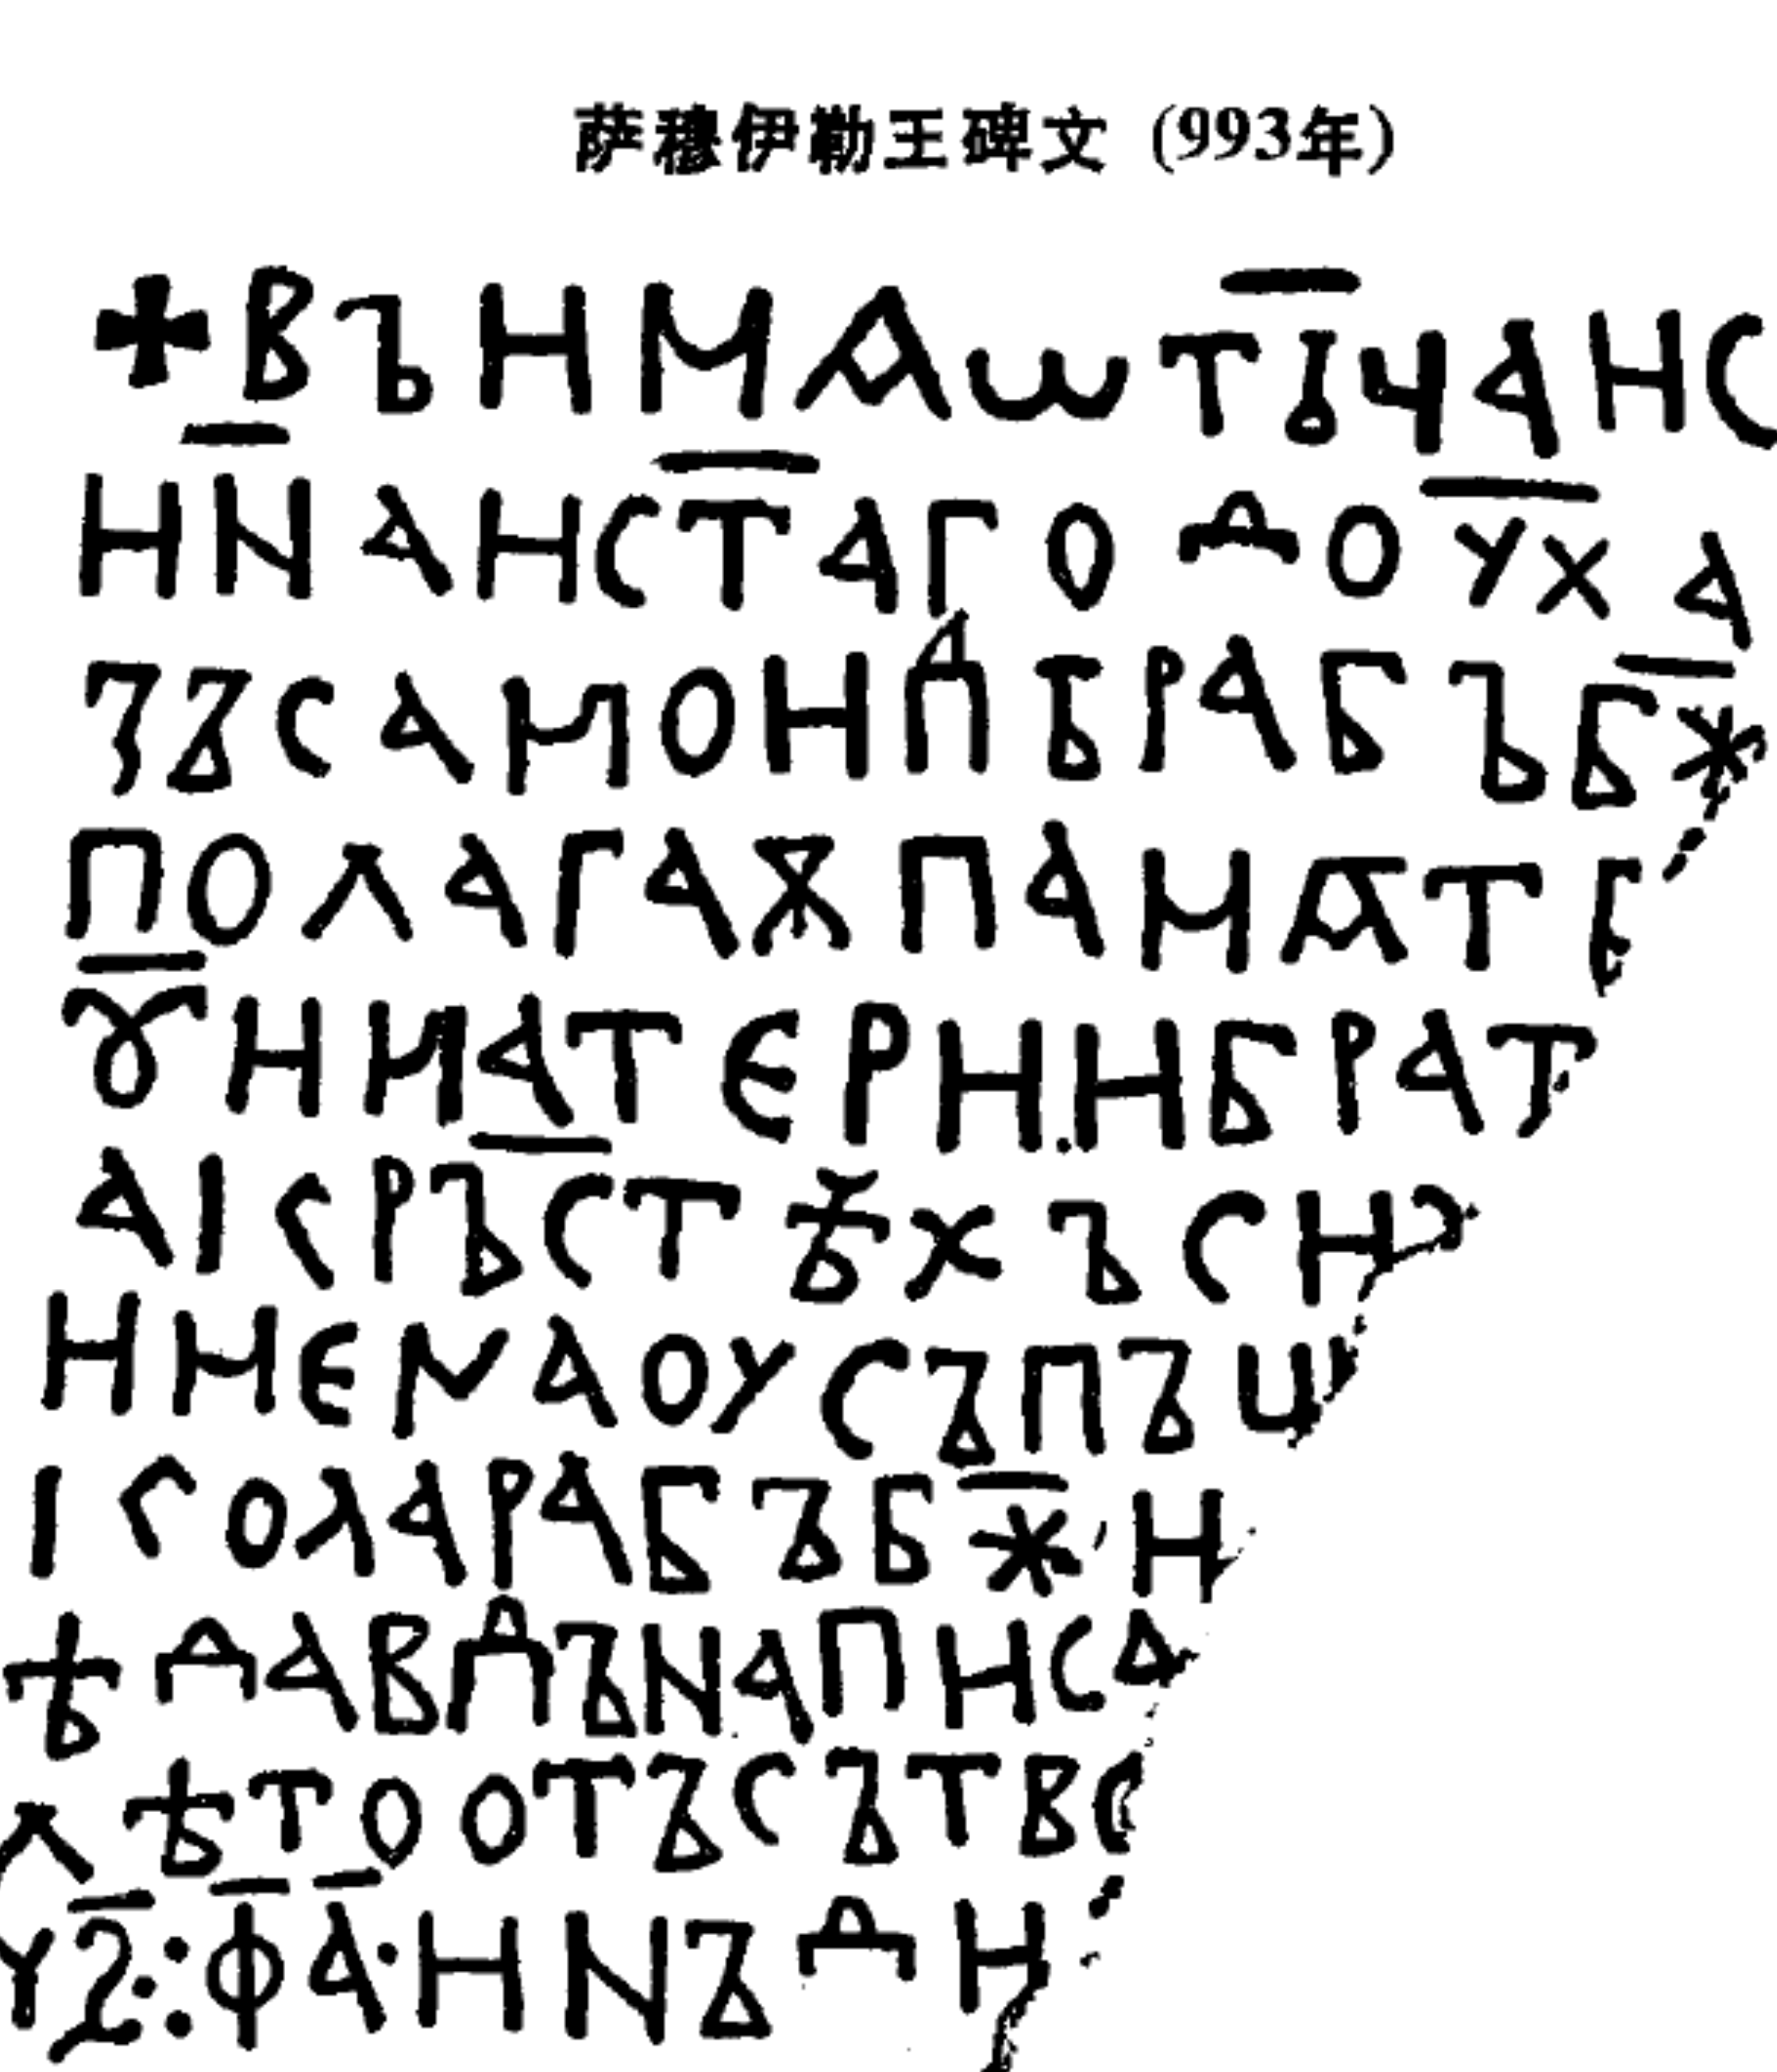
\includegraphics[width=0.72\textwidth]{samuel_inscription.png}
\caption*{萨穆伊勒王碑文（993 年）}
\end{figure}


\begin{figure}[htbp]
\centering
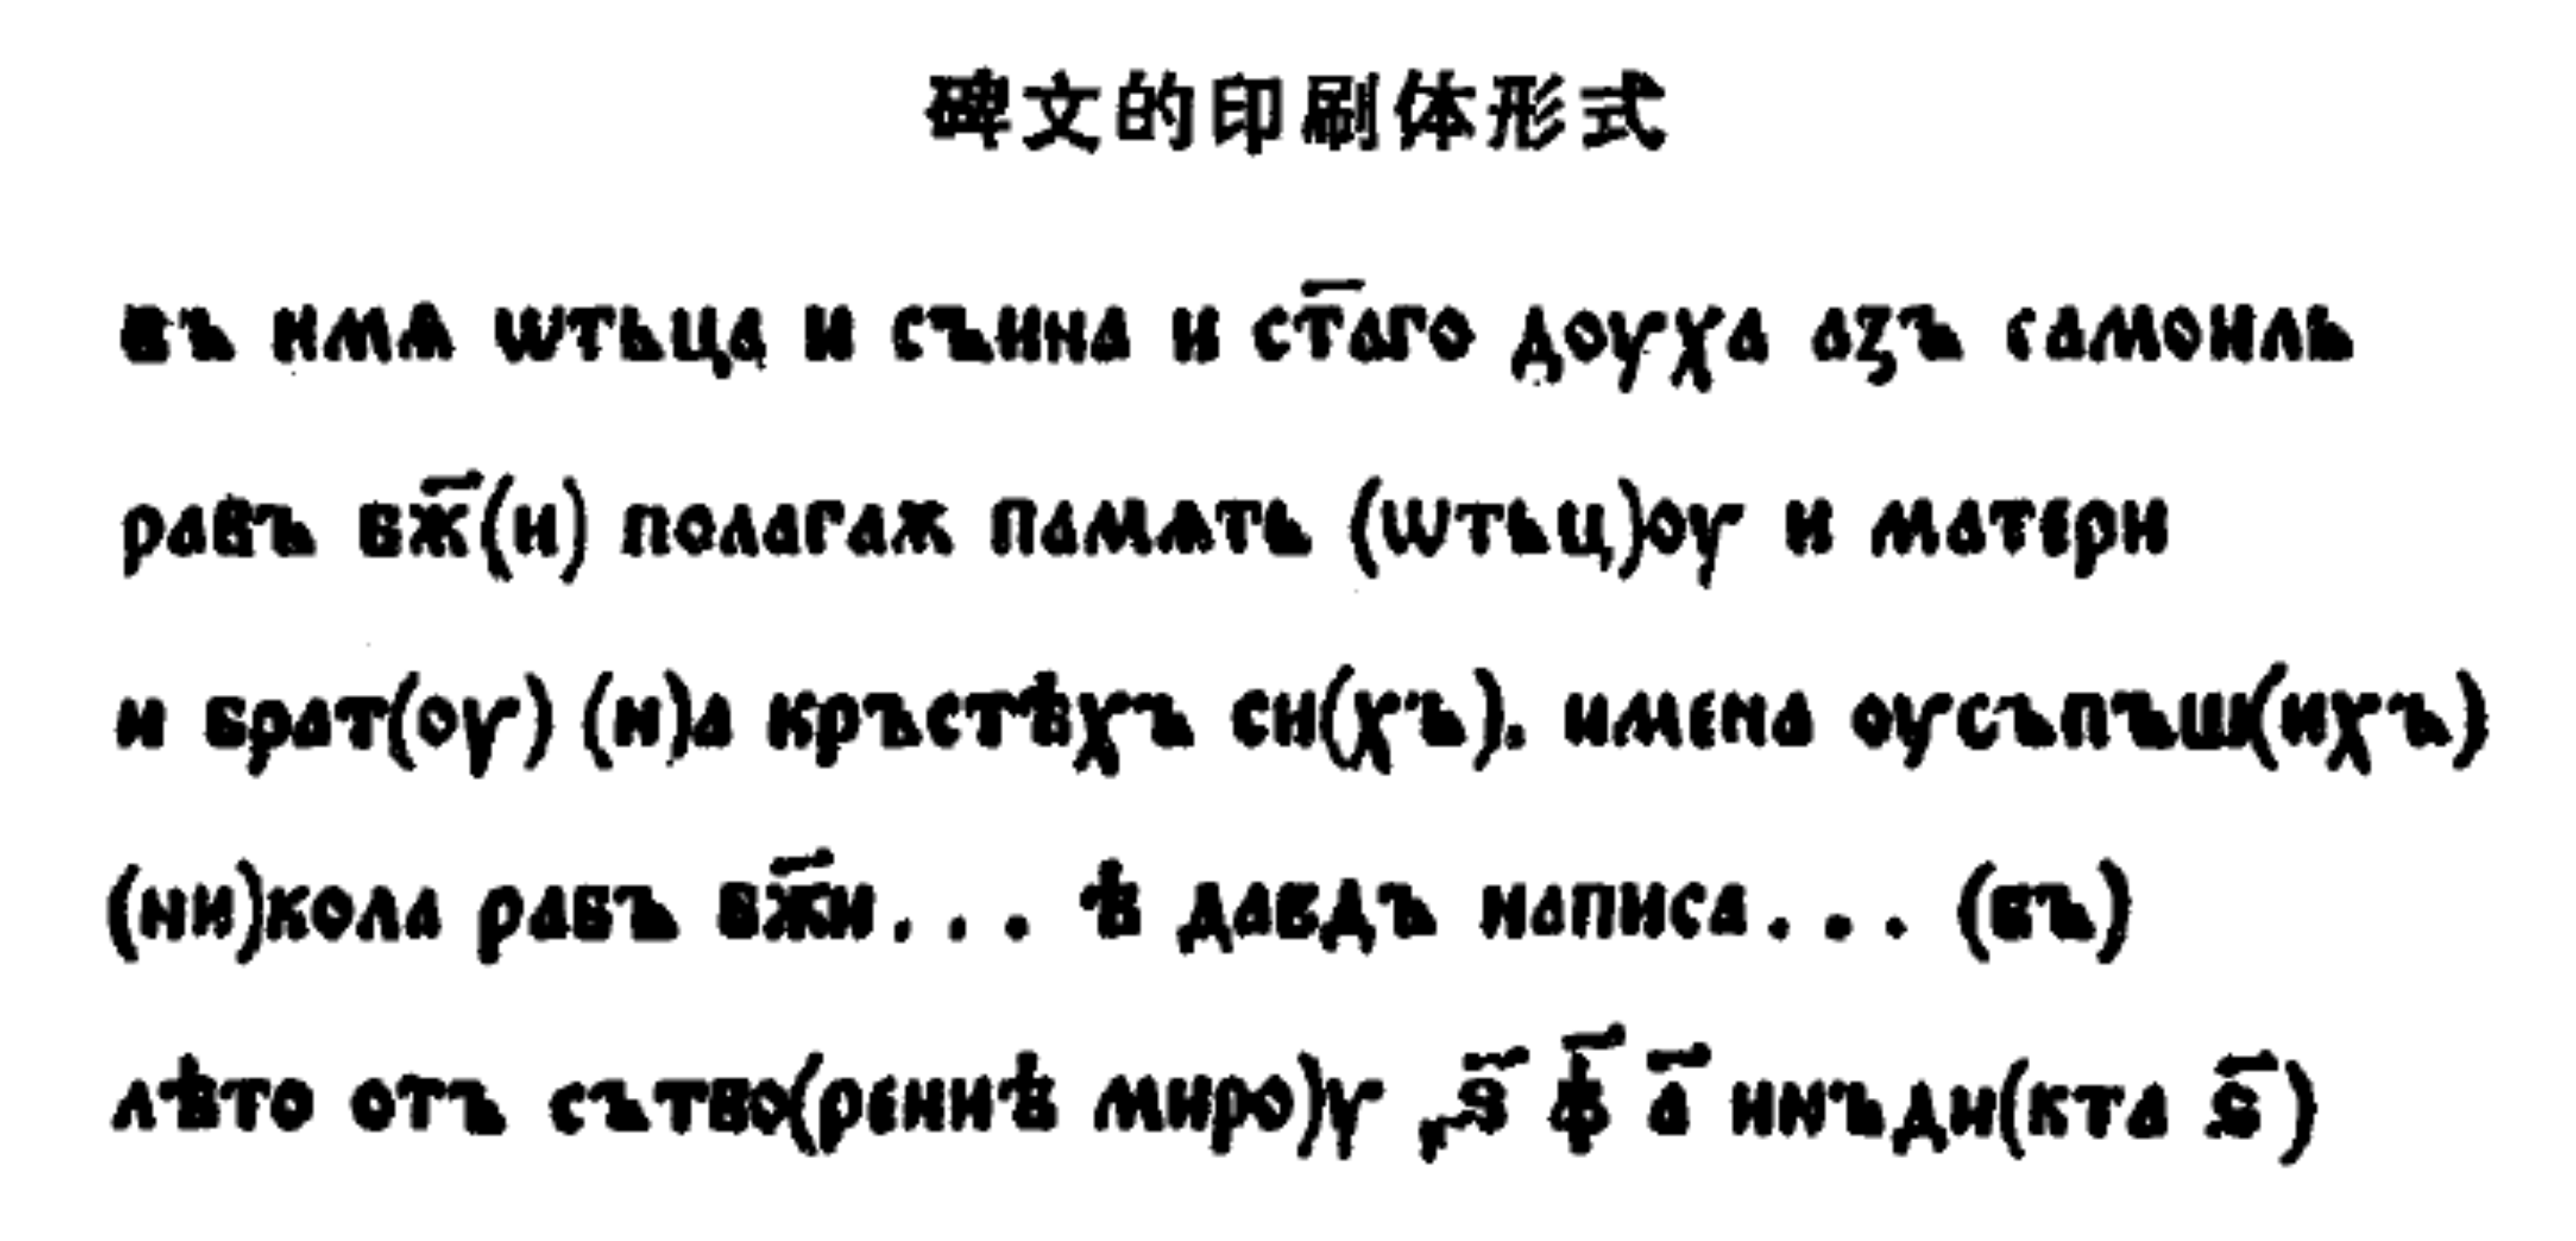
\includegraphics[width=0.94\textwidth]{samuel_printed_form.png}
\caption*{碑文的印刷体形式}
\end{figure}

\paragraph{《萨瓦书》}（\term{Саввина книга}）——基里尔文字。因附言中两次提到教士萨瓦（\term{Савва}），故名。11 世纪抄本。内容是福音书片断。语言特征：没有反映 \term{ъ, ь > o, e} 的变化，据认为此抄本产生于保加利亚东部。

\paragraph{《苏普拉斯利抄本》}（\term{Супрасльский кодекс}）——基里尔文字。19 世纪发现于波兰比亚韦斯托克附近的苏普拉斯利修道院，故名。共 285 面，抄成于 11 世纪保加利亚东部。语言特征：没有反映 \term{ъ > o} 的变化，但反映了 \term{ь > e} 的变化。

\paragraph{《奥斯特罗米尔福音书》}（\term{Остромирово евангелие}）——基里尔文字。1056--1057 年为诺夫哥罗德总督奥斯特罗米尔抄写的福音书，故名。共 294 面，第 25 面以前和以后为两人所抄。主要抄写者是助祭哥里戈利。语言特征：1）在抄辅音之间的音组“\term{р, л + ъ, ь}”时，如 \term{скрьбь}（悲哀）、\term{мрьтвь}（死去的），第二个抄写者通常忠于所依据的东保加利亚抄本，第一个抄写者则按东斯拉夫语（古俄语）读法写作 \term{скърбь, мьртвъ}；2）字母 \term{ѧ} 和 \term{оу} 混用，\term{ѫ} 和 \term{ю} 混用，\term{ѧ} 和 \term{ꙗ} 混用；3）动词变位第 3 人称词尾以 \term{-ть} 代替古斯拉夫语的 \term{-тъ}：\term{єсть}（〔他〕是）、\term{имѫть}（〔他们〕有；古斯 \term{єстъ, имѫтъ}）。总的看来，这是个俄罗斯版本的古斯拉夫语文献。有的学者认为这已不能算古斯拉夫语文献，而应视为古俄语文献了。

\origitem{2.1.6}
古斯拉夫语文献中反映的语言现象，可以为历史比较研究、重拟原始斯拉夫语（乃至原始印欧语）提供宝贵的资料。
\sourcepage{65}{83}
任何其他斯拉夫语的现存文献都比它晚：俄语的始见于 11 世纪，塞尔维亚语的始见于 12 世纪，捷克语的始见于 13 世纪，波兰语的始见于 14 世纪。\footnote{校勘：这里把“成篇文献”“本族语连续文本”和“任何书面记录”混为一谈，年代因口径不同会显著提前。例如捷克语的词语和句子见于 11--12 世纪拉丁文献，波兰语的人名、地名等斯拉夫语材料也早于 14 世纪；若只指较完整的连续文本，则原书所列年代才较接近传统教材口径。}


古斯拉夫语是一种过去各族斯拉夫人都能读懂的书面共同语（\term{koine}）。它在宗教活动中逐渐形成所谓教会斯拉夫语，在世俗活动中与各地口语结合，对现代标准语，特别是东、南两支斯拉夫标准语，产生过很大的影响。了解这种影响，有助于认识上述标准语的形成过程与特点。

古斯拉夫语作为一种经过加工的书面语，曾在一定历史时期通行于各族斯拉夫人之间；它不仅是传播宗教的工具，而且成为沟通文化、促进文明的媒介。因此要研究斯拉夫学（尤其是语言发展的历史），不能不懂得古斯拉夫语。

\section*{2. 字母与拼读}
\phantomsection\addcontentsline{toc}{section}{2. 字母与拼读}
\origitem{2.2.1}
下面是古斯拉夫语所使用的两种字母（见 66 页）：

\origitem{2.2.2}
现在对表中的基里尔字母作些说明。为了便于读者查找，我们在括号内指出字母在表中的位次。

以下 15 个字母与现代的写法相同或相近，读音一致，不必多加解释：\term{а(1), б(2), в(3), г(4), д(5); к(13), л(14), м(15), н(16); п(18), р(19), с(20), т(21)}。只有 \term{е(6), х(24)} 的笔划与现代的 \term{е, х} 略有不同；本书下文，为减少印刷困难起见，以现代的 \term{е, х} 代替。

\term{ж(7)} 是软音，必要时用 \term{ж′ [ž′]} 表示。

\term{ѕ, ꙃ(8)} 是同一字母的两种写法，都表示软塞擦音 \term{д′з′ [d′z′]}，在古斯拉夫语文献中互见：\term{кънѧѕь = кънѧꙃь}（大公、长官）。本书下文只用 \term{ѕ}。

\term{з, ꙁ(9)} 也是同一字母的两种变体，都读浊擦音 \term{[z]}。本书下文以现代的 \term{з} 代替。

\term{и(10)} 和 \term{і(11)} 在希腊语中曾表示两个不同的元音，\term{и} 表示 \term{i < ē}，\term{і} 表示固有的 \term{i}。这两个字母借入古斯拉夫语之后，读音相同，都是 \term{[i]}。本书下文以现代的 \term{и} 代替。


\sourcepage{66}{84}
\begin{figure}[p]
\centering
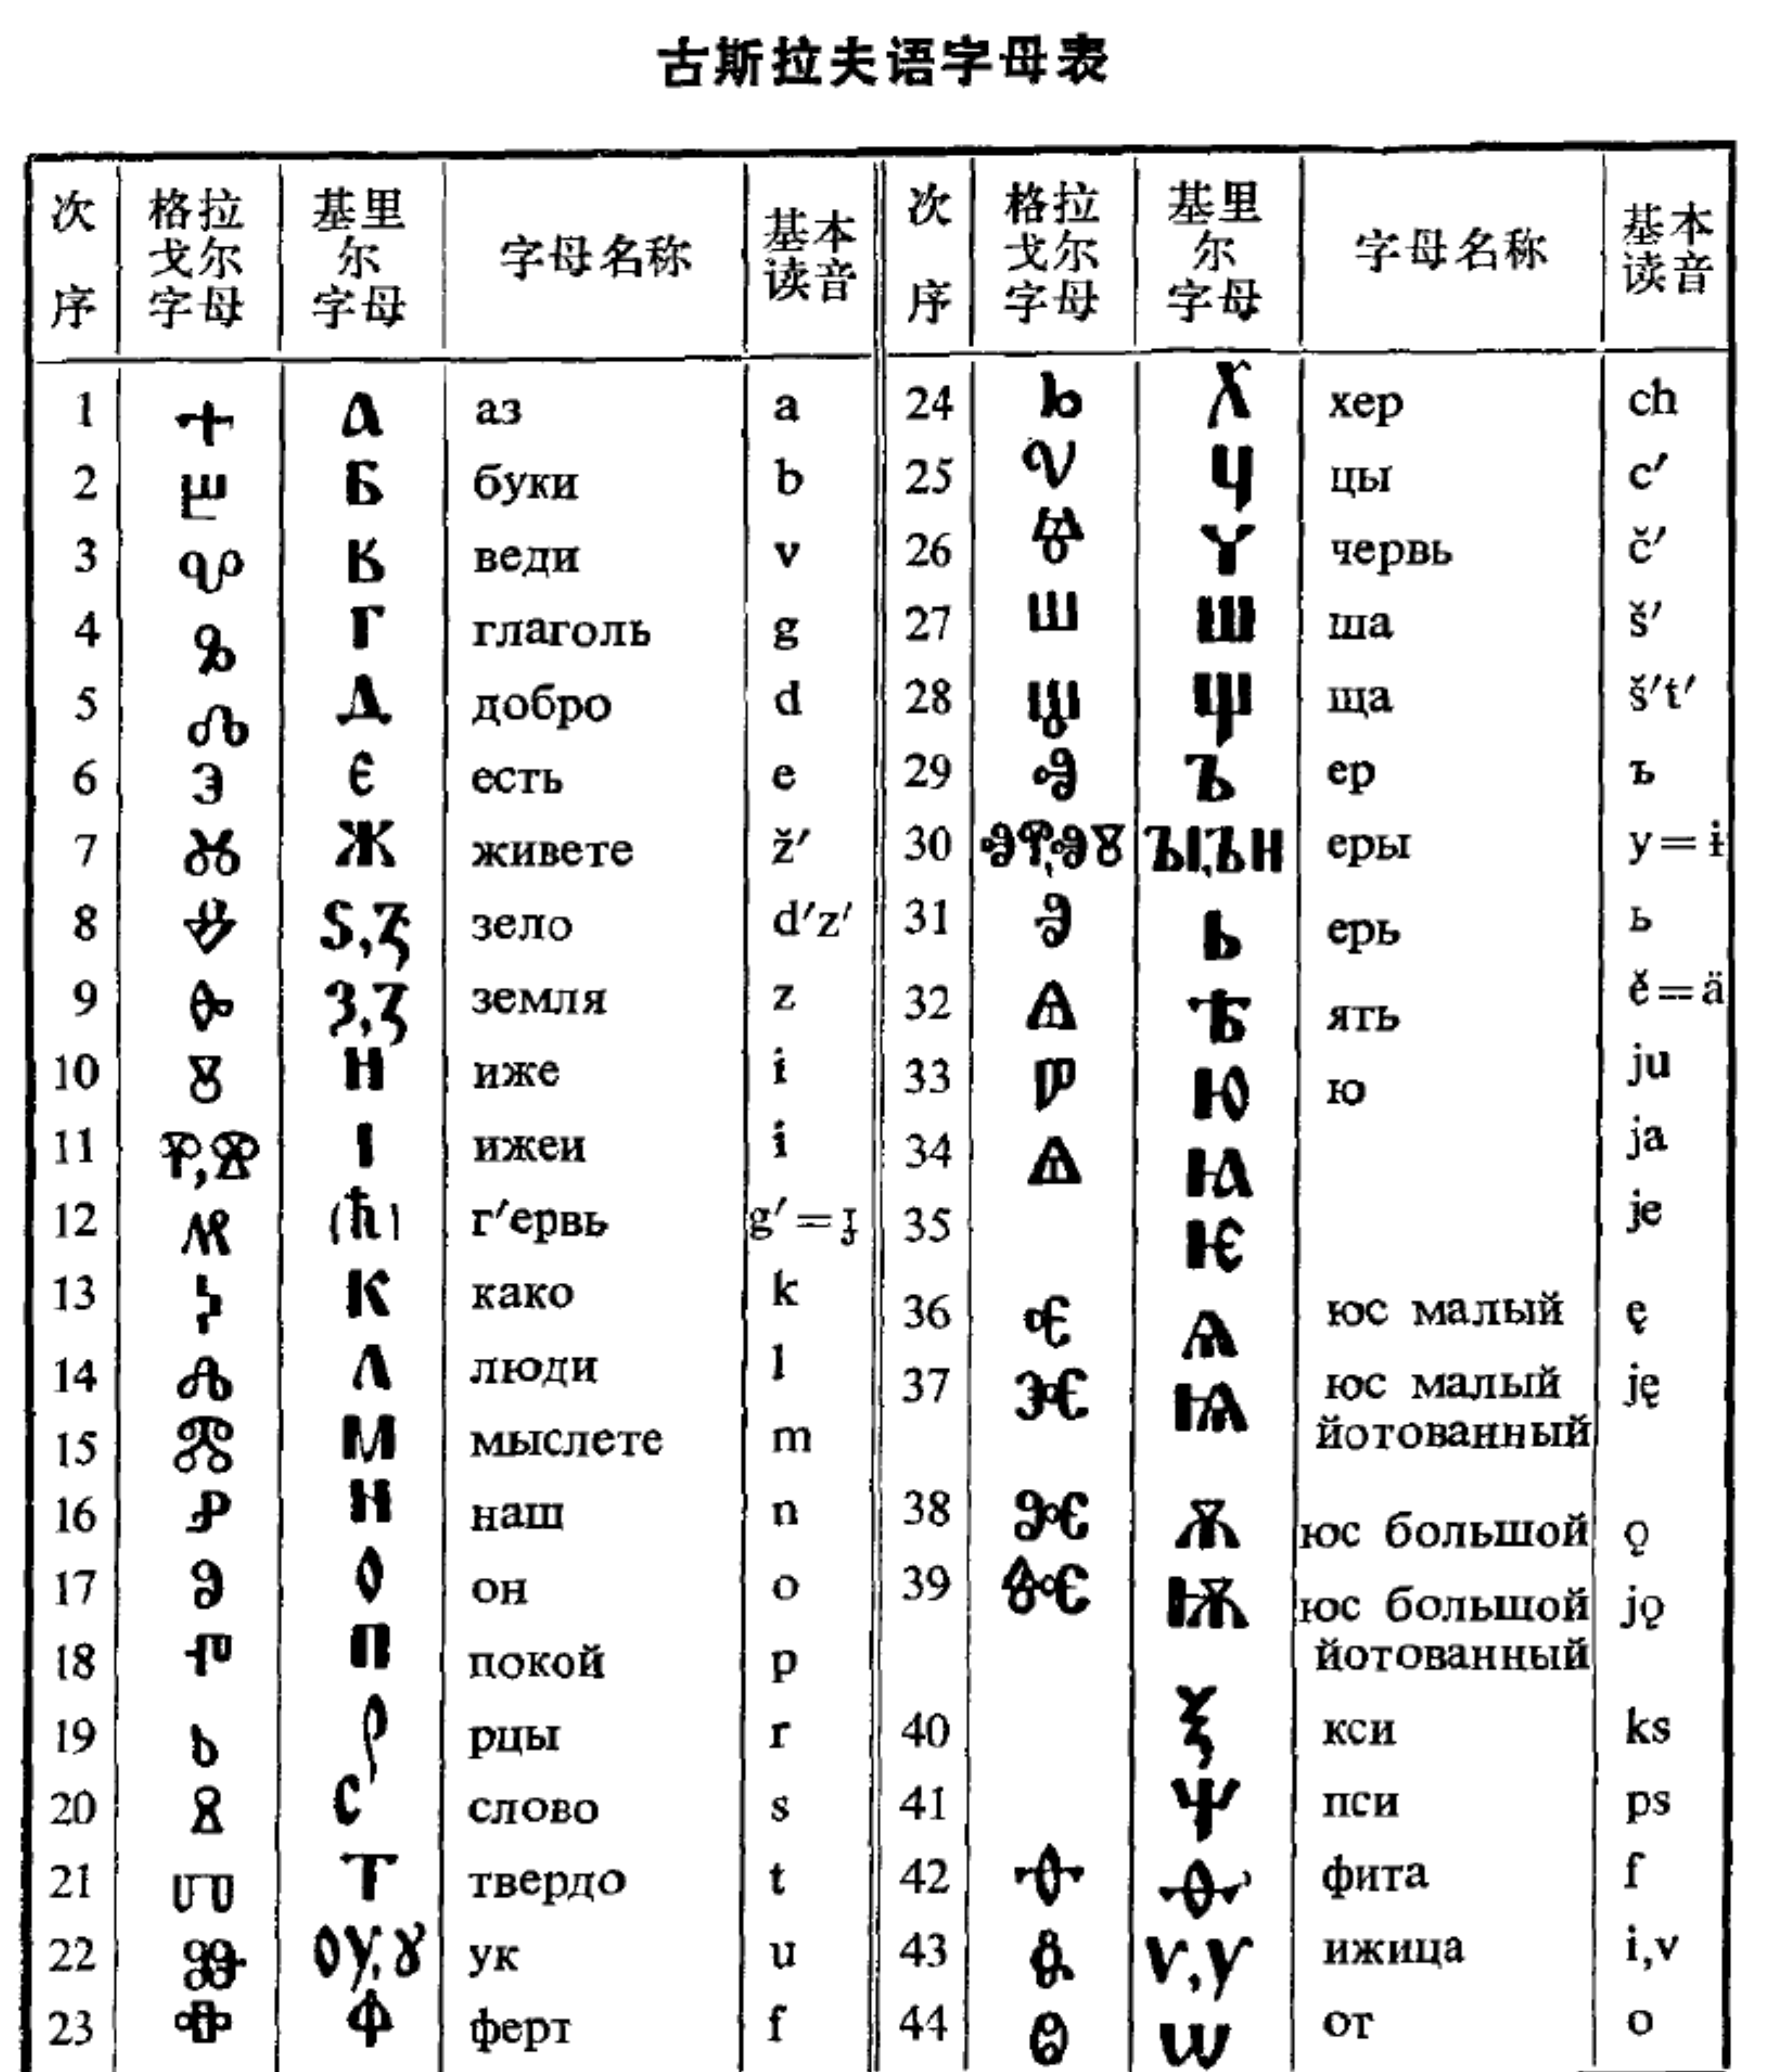
\includegraphics[width=\textwidth,height=0.82\textheight,keepaspectratio]{ocs_alphabet_table.png}
\caption*{古斯拉夫语字母表}
\end{figure}

\sourcepage{67}{85}
第 12 个字母只见于格拉戈尔抄本的个别外来词中，表示中舌（硬腭）浊塞音，相当于塞尔维亚语的 \term{đ}（国际音标 \term{[ɟ]}）；基里尔抄本中没有相应的字母。


\term{о(17)} 和 \term{ω(44)} 在希腊语中分别表示短元音 \term{o} 和长元音 \term{ō}，但在古斯拉夫语中没有长短之分，都读 \term{[o]}，只是 \term{ω} 通常见于希腊借词中，例如 \term{Иѡанъ}（约翰）、\term{Соломѡнъ}（所罗门）。

第 22 个字母也有两个变体，以 \term{оу} 两个字母表示一个单元音 \term{[u]} 是沿用希腊的传统写法，因为希腊语的 \term{u} 源于二合元音 \term{ou}。表中右侧的写法其实是上下合体字母，它常用于一行末尾。本书下文一律写作 \term{оу}。

\term{ф(23)} 和 \term{ѳ(42)} 在希腊语中的最初读音不同，前者是唇齿音 \term{[f]}，后者是送气的齿音 \term{[th]}，后来合并为 \term{[f]}，只是仍按传统写作两个字母。这两个字母在古斯拉夫语中读音相同，只用于外来词（多为希腊借词）中：\term{фарисеи}（法利赛人）、\term{Филиппъ}（菲力普）；\term{ѳома}（福马）、\term{ѳеодоръ}（费奥多尔）。本书下文一律写作 \term{ф}。斯拉夫语中本来没有 \term{[f]} 音，早期抄写者是随着书面语中的希腊词学会这个音的；一般人口语中常以 \term{п, в, т} 代替它。

\term{ц(25)} 和 \term{ч(26)} 是软塞擦音，分别记作 \term{ц′ [c′]}、\term{ч′ [č′]}。\term{ш(27)} 是软擦音 \term{ш′ [š′]}。\term{щ(28)} 是 \term{ш} 和 \term{т} 的合体字母，表示软 \term{ш′} 和软 \term{т′} 的复合音 \term{[š′t′]}（现代写 \term{щ}）。本书下文写作 \term{шт} 或 \term{щ}。古斯拉夫语中还有一个与之相对的浊音 \term{ж′д′ [d′žd′]}，不过没有专门的字母。

\term{ъ(29), ь(31)} 是 1.1.8 节中讲过的短弱元音。

第 30 个字母有两个变体 \term{ы} 和合体形式。左半边都是 \term{ъ}，右半边是元音字母 \term{і(11)} 或 \term{и(10)}；这个元音的一部分源于紧弱元音 \term{ŷ = ъ + i}（1.5.5）。本书下文一律写作现代的 \term{ы}。

\term{ѣ(32)}（= \term{ě < *ē}）表示较开的（舌位较低的）\term{e} 或二合元音 \term{ea}。

表中第 36、38 位分别表示 1.3.6 节中所讲的鼻元音 \term{ę, ǫ}，如 \term{пѧть}（五）、\term{пѫть}（路）；第 37、39 位则是相应的碘化鼻元音。为了减少排版的困难，本书一般以 \term{ę, ǫ} 及 \term{ję, jǫ} 来代替。

\sourcepage{68}{86}
\term{ю(33)} 以及表中第 34、35、37、39 位左侧的字形都可以分析为 \term{i + 相应元音}，表示音组“\term{j + 相应的元音}”；在辅音字母后表示“软辅音 + 相应的元音”。本书下文一般以 \term{ja, je, ję, jǫ} 来代替这些字母。


\term{ξ(40), ψ(41)} 以及表中第 43 位的希腊借词字母，多用于希腊借词中，如 \term{алеѯандръ}（亚历山大）、\term{ѱалъмъ}（赞美诗，圣歌）、\term{егѵпътъ}（埃及人）。第 43 位源于希腊语的 \term{υ}，表示圆唇前元音 \term{ü}（国际音标 \term{[y]}）的字母，在古斯拉夫语抄本中通常表示元音 \term{[i]}（如 \term{егѵпътъ}），偶尔在元音字母前表示唇齿浊辅音 \term{[v]}，如 \term{евангелие}（福音书）。

可以看出，当初设计基里尔字母时，除全部利用了希腊的 24 个字母外，还为适应斯拉夫语（9 世纪马其顿方言）的需要，创造了 10 多个字母。

\origitem{2.2.3}
古斯拉夫语抄本中还有一些常见的符号。其中比较重要的是加在辅音字母 \term{л, н, р} 上用来表示软音的“′”或弧线。同一个“意志”的几种写法读音相同，都含有软 \term{[l′]}：\term{[vol′a]}。同样，其宾格形式也可有几种写法。其他例：\term{н′ива}（田地），\term{кон′ь}（马），\term{мор′е}（海）。

古文献中还常用略语符（\term{титло <} 希腊 \term{τίτλος}）：\term{снъ = сынъ}（儿子），\term{чкъ = человѣкъ}（人），\term{оцъ = отьць}（父亲）。

此外，古斯拉夫语还按照拜占廷习惯用字母表示数目，此时字母上也加略语符，同时在左右两侧各加一个点：带点和略语符的相应字母分别表示 \term{1} 和 \term{100}。这里不拟一一详述。

\section*{3. 语音}
\phantomsection\addcontentsline{toc}{section}{3. 语音}


\origitem{2.3.1}
古斯拉夫语共有 38 个音位：11 个元音，27 个辅音（不包括 \term{ф}）。


\begin{center}
\begin{tabularx}{0.72\textwidth}{>{\bfseries}l *{3}{>{\LingFont\centering\arraybackslash}X}}
\toprule
 & 前元音 & 央元音 & 后元音\\
\midrule
\sourcepage{69}{87}
高（闭）元音 & и & ы & оу\\
中元音 & е，ѧ，ь &  & ъ，о，ѫ\\
低（开）元音 & ѣ &  & а\\
\bottomrule
\end{tabularx}
\end{center}

\begin{center}
\begin{tabularx}{0.94\textwidth}{>{\bfseries}l *{5}{>{\LingFont\centering\arraybackslash}X}}
\toprule
 & 双唇音 & 唇齿音 & 前舌音 & 中舌音 & 后舌音\\
\midrule
塞音 & п，б &  & т，д &  & к，г\\
擦音 &  & (ф)，в & с，з；с′，з′；ш′，ж′ & j & х\\
塞擦音 &  &  & ц′，ѕ′[д′з′]；ч′ &  & \\
复合音 &  &  & щ[ш′т′]，ж′д′ &  & \\
鼻音 & м &  & н；н′ &  & \\
流音 &  &  & л，р；л′，р′ &  & \\
\bottomrule
\end{tabularx}
\end{center}

\origitem{2.3.2}
\term{ѫ, ѧ} 是鼻元音，其余都是非鼻元音。\term{о, оу [u], ѫ} 是唇元音，其余都是非唇元音。

\term{ъ, ь} 两个短弱元音是非全值元音，其余都是全值元音。不过 \term{ы, и} 例外：它们通常是全值元音，但在 \term{j} 或 \term{и} 前时可以是非全值元音（2.3.6）。

\sourcepage{70}{88}
从元音同前方辅音结合的特点看，重要的是前元音 \term{и, е, ѧ, ь, ѣ} 与非前元音的对立。前元音前的辅音只能是软的或半软的；非前元音 \term{ы, ъ, о} 前的辅音只能是硬的，不能是软的或半软的；后元音 \term{а, ѫ, оу} 前的辅音既可能是硬的，也可能是软的，但不能是半软的。

词首这个位置对元音有一定的限制。这里从来不出现 \term{ы, ъ, ь}，也很少见到 \term{ѧ, ѣ}。某些词开头的 \term{а, оу} 有时写作相应的碘化字母，读音不同，但词义不变：\term{азъ} — 碘化写法（我），\term{оутро — ютро}（早晨）。


\origitem{2.3.3}
辅音中清浊对立的有 \term{п--б, т--д, к--г, с--з, с′--з′, ш′--ж′, ш′т′--ж′д′}。由于开音节规律的关系（1.3.1--1.3.3），辅音不能出现在词末，词内部也没有清浊噪辅音相邻的组合，所以当时还没有现代斯拉夫语中普遍存在的清浊同化规律。

例外主要是前缀 \term{без-, въз-, из-, раз-} 和前置词末尾的 \term{-з}。当后面遇到以清音开始的词或词根时，\term{з} 被同化为清音 \term{с [s]}：\term{бес плода}（没有果实）、\term{въсходъ}（升起）、\term{ис корабля}（从舰船内）、\term{ископати}（挖遍）、\term{растачати}（驱散）。

\origitem{2.3.4}
辅音中硬软对立的有 \term{н--н′, л--л′, р--р′, с--с′, з--з′}。

软音 \term{н′, л′, р′} 分别来源于 \term{nj, lj, rj}：\term{кон′ь}（马）$<$ \term{*konjos}，\term{пол′е}（田地）$<$ \term{*poljon}，\term{мор′е}（海）$<$ \term{*morjon}，\term{гон′ѫ}（〔我〕追赶）$<$ \term{*gonjǫ}，\term{вел′ѫ}（〔我〕命令）$<$ \term{*veljǫ}，\term{дар′ѫ}（〔我〕赠给）$<$ \term{*darjǫ}（1.4.5 之 1）。软音 \term{с′, з′} 是后舌音 \term{х, г} 受前元音软化而成：\term{вьсь}（整个的）、\term{доуси}（\term{доухъ} “精灵”的复主）、\term{дроузи}（\term{дроугъ} “朋友”的复主）、\term{кънѧзь}（大公）（1.4.3--1.4.4）。

后舌音 \term{г, к, х} 只能是硬音，从不出现在前元音前。例外只限于个别希腊借词：\term{Георгий}（乔治）、\term{кедрь}（雪松）、\term{архиереи}（主教）；这时后舌音是半软的。

\term{ш′, ж′, ц′, ч′, ш′т′(щ), ж′д′, ѕ′(д′з′)} 和 \term{j} 都是非对偶型的软音。除 \term{j} 外，其余都是在原始斯拉夫语时期因软化而产生的（1.4.2--1.4.5），通常称之为“固有软音”。它们大都不能出现在 \term{ы, ъ, о, ѣ} 前；只有 \term{ц′, ѕ′} 例外，可用于 \term{ѣ} 前：\term{цѣна}（报仇），\term{ѕѣло}（很）。\term{j} 没有专门的字母表示，当在词首或元音后时用相应的碘化元音字母表示。

\term{п, б, т, д, в, м} 是无对偶型的硬音，即没有相应的软音。


\sourcepage{71}{89}
凡硬音位于前元音前时，都变为半软音（随位变体）：\term{пити}（喝）、\term{раби}（“奴隶”，复主）、\term{текѫ}（〔我〕流动）、\term{идеть}（〔他〕走）、\term{везѫ}（〔我〕运载）、\term{метѫ}（〔我〕揉皱）。上文提到的硬音 \term{н, л, р, с, з} 和 \term{г, к, х}（在外来词中）位于前元音前时同样是半软音。

\origitem{2.3.5}
古斯拉夫语文献中（至 11 世纪末）反映出来的主要语音变化有：短弱元音 \term{ъ, ь} 的消亡；紧弱元音 \term{ŷ, î} 的演变；成节流音的消长；固有软音的硬化。

\term{ъ, ь} 有了强弱位的区别。在强位上 \term{ъ > o, ь > e}：\term{дъждь}（雨）$>$ \term{дождь}，\term{събьрати}（收集）$>$ \term{собрати}，\term{дьнь}（天，日）$>$ \term{день}，\term{коньць}（末端）$>$ \term{конецъ}，\term{тьмьна}（黑暗的，阴性）$>$ \term{темьна}。弱位上的 \term{ъ, ь} 消失了：\term{къто}（谁）$>$ \term{кто}，\term{чьто}（什么）$>$ \term{что}，\term{кънига}（书）$>$ \term{книга}，\term{придеть}（〔他〕要来）$>$ \term{придет}。

这条规律也适用于在非成节流音 \term{р, л} 后、另一辅音前的 \term{ъ, ь}（参看 2.3.6 末段），就是说音组 \term{ръ, лъ, рь, ль} 中的 \term{ъ, ь} 在强位上也变为 \term{o, e}，在弱位上也消失了：\term{кровь}（血），\term{крестъ}（十字架），\term{плоть}（肉体），\term{слезъ}（眼泪，复属）；\term{крве, крета, плоти}（以上皆是单数属格），\term{слза}（单主）。

\term{ъ, ь} 的演变在绝大多数古斯拉夫语文献中都有不同程度的反映。但在现存最古的抄本《基辅残篇》中，\term{ъ, ь} 的变化基本上没有反映，这可能是 10 世纪末抄写此文献时这一变化尚未发生的原故，虽然不能排除地域方言（摩拉维亚）的影响。至于没有反映 \term{ъ, ь} 变化的晚期文献，如《奥斯特罗米尔福音书》（1056--1057 年），则说明在抄录该文献的东斯拉夫地区，\term{ъ, ь} 消失得比较晚。

\origitem{2.3.6}
上文说过，字母 \term{ы, и} 除表示全值元音外，还可以表示紧弱元音；为便于区别，本书用 \term{ŷ, î} 表示。

\term{ŷ, î} 有两个来源（1.5.5）。一个是 \term{ъ, ь} 受后面 \term{j} 或 \term{и (< *jь)} 同化而形成的：

\begin{center}
\begin{tabularx}{0.78\textwidth}{>{\LingFont}X >{\LingFont}c >{\LingFont}X >{\raggedright\arraybackslash}X}
\toprule
原组合 &  & 结果 & 词义\\
\midrule
новъ + и（\term{< *jь}） & \term{>} & новŷи & 新的\\
добръ + и（\term{< *jь}） & \term{>} & добрŷи & 好的\\
синь + и（\term{< *jь}） & \term{>} & синîи & 蓝色的\\
\sourcepage{72}{90}
кость + и（\term{< *jь}） & \term{>} & костîи & “骨头”，复属\\
\bottomrule
\end{tabularx}
\end{center}


另一个来源是全值元音 \term{ы, и} 受 \term{j} 或 \term{и} 同化而成的。例如，\term{ы, и} 在不定式 \term{мыти}（洗）、\term{крыти}（覆盖）、\term{бити}（打）、\term{шити}（缝）中是全值元音，而在人称形式和命令式中（即在 \term{j} 或 \term{и} 前）则变为紧弱元音：

\begin{center}
\begin{tabularx}{0.76\textwidth}{>{\bfseries}l *{3}{>{\LingFont\centering\arraybackslash}X}}
\toprule
 & 单 1 人称 & 单 2 人称 & 命令式\\
\midrule
“洗” & мыjѫ & мыjеши … & мŷи\\
“打” & биjѫ & биjеши … & бîи\\
\bottomrule
\end{tabularx}
\end{center}

\term{ŷ, î} 的发音虽然比全值元音 \term{ы, и} 短促，但音值相近，所以古文献中既用字母 \term{ы, и} 表示，也用 \term{ъ, ь} 表示：\term{новыи, новъи, новы}；\term{синии, синьи, сини}；\term{костиjѫ, костьjѫ} 等。

紧弱元音 \term{ŷ, î} 的演变结果不同于全值的 \term{ы, и}。在古斯拉夫语中，它们也像 \term{ъ, ь} 一样有强位、弱位之分。强位指在重读音节中或在词末的 \term{и (< *jь)} 前；弱位指后一音节有全值元音的位置。

后来，弱位上的 \term{ŷ, î} 消失了。关于 \term{ŷ} 消失的过程，古文献中没有直接的例证；\term{î} 的消失在各文献中却反映得很清楚。

\term{î} 消失后的写法有三种。第一种是把原来的 \term{и} 改写作 \term{ь}，如 \term{каменье}（石头）、\term{бьенъ}（“打”，被动形动词）、\term{змьjѫ}（“蛇”，单宾）、\term{паданъемъ}（“跌落”，单工）。第二种是改作 \term{ъ}，如 \term{бытье}（存在）、\term{ноштъjѫ}（“夜”，单工）、\term{зъванье}（称号）、\term{достоинье}（财产）；这里的 \term{ъ, ь} 已不表示任何元音，只表示辅音后有个 \term{j} 了。第三，是仍按传统习惯写作 \term{и}，但这个 \term{и} 并不反映实际发音（元音 + \term{j}），证据是其前一音节中的短弱元音 \term{ъ, ь} 转为强位，变成全值元音了：\term{шествие}（“行进”），\term{лестиjѫ}（“阿谀”，单工），\term{любовиjѫ}（“爱”，单工）。

\sourcepage{73}{91}
强位上的 \term{ŷ, î} 在古斯拉夫语以及现代各斯拉夫语中都同全值元音 \term{ы, и} 合流，只有俄语的 \term{ŷ, î} 变为 \term{o, e}（同 \term{ъ, ь} 一样；参看 1.5.5）。


\origitem{2.3.7}
流音 \term{р, л} 有时表示普通的辅音，但在辅音之间时可以表示成节音，即构成音节的核心。成节流音在古文献中没有专门的字母表示，而是写作 \term{ръ, рь, лъ, ль}：\term{гръло}（咽喉）、\term{скрьбь}（悲哀）、\term{тръгъ}（交易）、\term{прьвъ}（第一）、\term{съмрьть}（死亡）、\term{зрьно}（谷粒）、\term{чрьвь}（蠕虫）；\term{длъгъ}（长的）、\term{влъкъ}（狼）、\term{плънь}（充满的）。这里的 \term{ъ, ь} 并不表示元音，而只标示 \term{р, л} 的成节功能，可分别转写为 \term{r̥, l̥}。

因此古文献中经常把 \term{р, л} 后的 \term{ъ, ь} 混用：\term{гръло = грьло}，\term{чрьвь = чръвь}，\term{длъгъ = дльгъ}，\term{влъкъ = влькъ}。

不过，夹在辅音字母之间的 \term{ръ, рь, лъ, ль} 并不都表示成节流音。有时它们只表示“非成节流音 \term{р, л +} 短弱元音 \term{ъ, ь}”：\term{кръвь}（血）、\term{крьстъ}（十字架）、\term{блъха}（跳蚤）、\term{плъть}（肉体）、\term{сльза}（泪）。这类词里的 \term{ъ, ь} 表示元音，所以极少混淆；这类音组的演变结果也不同于成节流音。

成节流音源于史前期辅音之间的音组 \term{*ъr, *ьr, *ъl, *ьl}（参看 1.3.4），这些音组的音节核心是 \term{r̥, l̥}。在早期古斯拉夫语抄本中，\term{ръ, рь, лъ, ль} 不仅表示流音成节，而且表示伴随它们的元音成分有区别；《基辅残篇》（10 世纪）中的四种写法是不相混淆的。非成节的元音成分 \term{ъ, ь} 消失以后，成节流音 \term{ръ, рь} 才合并为一个 \term{[r̥]}，\term{лъ, ль} 也合并为 \term{[l̥]}，于是出现 \term{ъ, ь} 混用：\term{прьвъ -- пръвъ}（第一个）、\term{срьдьце -- сръдьце}（心）、\term{длъгъ -- дльгъ}（长久）。更加确凿的例证，是干脆把 \term{ъ, ь} 略去：\term{срдьце}（心）、\term{о цркьви}（关于教堂）、\term{тврдь}（硬的）、\term{съмрти}（“死亡”，单属）。

\sourcepage{74}{92}
这里的非成节元音成分 \term{ъ, ь} 的消失，不同于弱位短弱元音的消失。后者消失后能使前一音节中的 \term{ъ, ь} 转为强位而变成全值元音 \term{o, e}；前者则不能，因为 \term{r̥, l̥} 本身是音节核心，起全值元音的作用，它们使前一音节中的 \term{ъ, ь} 处于弱位而消失：\term{съмрьть > смрт′}（死亡），\term{съмрьти > смрти}（单属），\term{въ съмрьти > во смрти}（关于死亡）。


此外，古文献中还有一个所谓的“再生性成节流音”。在上文提到过的“非成节流音 \term{r, l +} 短弱元音 \term{ъ, ь}”的音组中，\term{ъ, ь} 在强位上变为 \term{o, e}，在弱位上消失，并使前一音节的 \term{ъ, ь} 转为强位而变为 \term{o, e}。但 \term{ъ, ь} 消失后，夹在辅音之间的 \term{р, л} 又逐渐获得成节功能，结果使这些词里也出现 \term{ъ, ь} 混淆的写法：\term{кръста}（本作 \term{кръста}，“十字架”，单属）、\term{крьви}（本作 \term{кръви}，“血液”，单属）、\term{слъзы}（本作 \term{сльзы}，“眼泪”，复主）、\term{пльти}（本作 \term{плъти}，“肉体”，单属）。最有说服力的佐证，是不止一种抄本中有略去 \term{ъ, ь} 的写法：\term{крста, крститель}（“施洗礼者”，单、位）。

这样一来，便产生了同词异干现象：\term{крест}（单主）-- \term{крста}（单属），\term{плот′}（单主）-- \term{плти}（单属）。后来异干趋向统一，带再生性成节流音的词干推广到该词的所有形式中。一方面是由于固有成节流音（\term{гръло, длъгъ}）的类推作用，另一方面可能是因为间接格 \term{крста, плти} 在口语中比主格 \term{крест, плот′} 常用。这个异干趋同的渐变过程，在抄本中表现为 \term{ъ--ь} 的混用和省略：\term{крьстъ -- кръстъ -- крстъ} 互见。

\origitem{2.3.8}
古斯拉夫语中的软音 \term{ж, ш, ч, ц, ѕ(=д′з′), жд, шт, с′, р′} 以及软唇音后的插入音 \term{л′}，后来大都硬化，有的则消失了。这些演变过程在文献中都有反映。

上文说过，\term{ж, ш, ч, ц, ѕ, жд, шт} 是固有软音，没有相对的硬音，后面不能出现非前元音 \term{ъ, о, ы}（反过来说，这些元音前只能出现硬音，2.3.4）。但文献中很早就有把上述辅音后的 \term{ь} 写成 \term{ъ} 的例子，也有时而写 \term{ь}、时而写 \term{ъ} 的摇摆现象：\term{длъжьнъ}（对……负债）$>$ \term{длъжънъ}，\term{длъжьникъ}（债务人）$>$ \term{длъжъникъ}，\term{шьдъ}（“行走”，过去时形动词阳性）$>$ \term{шъдъ}，\term{пришьли}（“来”，过去时形动词复数）$>$ \term{пришъли}，\term{начьнѫ}（〔我〕开始）$>$ \term{начънѫ}，\term{жрьбьць}（马驹）$>$ \term{жръбецъ}，\term{тъштьно}（讨厌）$>$ \term{тъштъно}。这些例子说明，上述软音在抄录相应文献的年代正在渐渐变成硬音。

\sourcepage{75}{93}
软塞擦音 \term{ѕ′ [д′з′]} 后来在各地域方言中都失去了开头的塞音成分，\term{д′з′ > з′}，最终变成了硬的 \term{з}。


固有软音 \term{с′, р′} 也逐渐变为硬音。例如：把 \term{вьсь}（整个的，所有的），\term{вьсѧ}（阴宾），\term{вьси}（复主），改写为 \term{вьсъ, вьсѧ, вьса} 之类的例子，就说明词干的尾辅音硬化了：\term{вьс′- > вьс-}；把 \term{пастырь}（牧师），\term{цѣсарь}（国王），\term{морю}（“海”，单与）改写为 \term{пастыръ, цьсаръ, мороу} 等例子，则说明 \term{р′ > р}。

总起来看，在 9 世纪古斯拉夫语的固有软音中，除去 \term{j, н′, л′} 之外，后来都硬化了。

稍有不同的是唇辅音与 \term{j} 之间的插入音 \term{л′}（1.4.5 之 5）。这个 \term{л′} 在 10 世纪的古斯拉夫语文献（如《基辅残篇》）中见于所有按语音规律应该出现的位置上。但 11 世纪文献中却只保留了词首的 \term{л′}：\term{блюдо}（桌子，菜肴），\term{блюсти}（遵守），\term{плюнѫти}（吐）；其余位置上的 \term{л′} 消失了：\term{землѧ}（“土地”，单属）$>$ \term{земѧ}，\term{земли}（单与），\term{корабль}（舰船）$>$ \term{корабь}，\term{каплѧ}（滴）$>$ \term{капѧ}。在现代保加利亚语和马其顿语方言中，非词首的插入音 \term{л′} 也未能保留，比较：保 \term{блюдо}，但 \term{земя} — 俄 \term{блюдо, земля}，塞 \term{bljȕdo, zèmlja}。



\section*{4. 语法}
\phantomsection\addcontentsline{toc}{section}{4. 语法}

\origitem{2.4.1}
根据 9--11 世纪文献判断，古斯拉夫语中有名词、形容词、数词、代词、动词、副词、前置词、连接词、语气词、感叹词等词类。名词、形容词、数词合称“静词”，与动词相对立；代词在形态上接近静词。静词的主要形态变化是变格，动词的主要形态变化是变位，只有一部分动词形式（如形动词）按变格变化。当时的形态变化比任何一种现代斯拉夫语都复杂。

\sourcepage{76}{94}
变格分为名词性变格和代词性变格。形容词既有名词性变格，也有代词性变格，两者意义和用法不同。名词共有七个格：主格、属格、与格、宾格、工具格、位格、呼格。其中属格由原始印欧语的属格与夺（离）格合并而来；表示处所的位格可以独立使用，不一定和前置词连用。呼格只是用于呼唤、称谓的特殊形式，严格地说并不表示词与词之间的语法关系，不过习惯上仍同其他变格形式一起说明。呼格的独立形式只见于阳性、阴性名词单数，其余情况下以主格形式兼作呼格。

古斯拉夫语有三个语法性：阳性、阴性、中性；三个数：单数、复数、双数。


双数表示两个或成双成对的事物。例如：\term{оученикъ}（弟子、学生）-- \term{дъва оученика}（两个弟子），\term{нога}（脚、腿）-- \term{дъвѣ нозѣ}（两脚、双腿），\term{око}（眼睛）-- \term{очи}（两眼），\term{оухо}（耳朵）-- \term{оуши}（双耳）。即使不加数词 \term{дъва / дъвѣ}（二），名词词尾本身也可以表示双数。

《美多迪传》记载拜占廷皇帝迈克尔三世派遣美多迪和君士坦丁出使摩拉维亚时曾说：\term{Вы бо јеста селоунѧнина, да селоунѧне вьси чисто словѣньскы бесѣдоуютъ.}（你们〔两人〕是索伦人，〔所有〕索伦人的斯拉夫语都讲得很好。）其中 \term{јеста селоунѧнина} 是双数主格，后半句主语 \term{селоунѧне} 则是复数主格。双数范畴不仅名词有，形容词、代词、动词和部分数词形式中也有。双数只有三组不同的词尾：主格与宾格同形，属格与位格同形，与格与工具格同形。

现代斯拉夫语大都失去双数范畴，只有斯洛文尼亚语和索布语至今还保留着。

\subsection*{a) 名词}
\origitem{2.4.2}
古斯拉夫语名词变格分为六类，分别以古代词干最后一个元音或辅音命名：
\begin{enumerate}[leftmargin=2.2em]
\item \term{ā} 类：古代词干以 \term{-ā (> -a)} 结尾，如 \term{жена}（女人）、\term{землја [zemlʹa]}（土地）。
\sourcepage{77}{95}
\item \term{ŏ} 类：古代词干以 \term{-ŏ (> -o)} 结尾，如 \term{рабъ}（奴仆）、\term{конь}（马）、\term{село}（村庄）、\term{полје [polʹe]}（田地）。
\item \term{ū} 类：古代词干以 \term{-ū (> -ъ)} 结尾，如 \term{сынъ}（儿子）。
\item \term{ī} 类：古代词干以 \term{-ī (> -ь)} 结尾，如 \term{гость}（客商）、\term{кость}（骨头）。
\item 辅音类：古代词干以 \term{-n, -s, -t, -r} 结尾，如 \term{дьнь, камы, имѧ, слово, телѧ, мати}。
\item \term{ū̄} 类：古代词干以 \term{-ū̄ (> -ы)} 结尾，如 \term{свекры}（婆母）、\term{црькы}（教堂、教会）。
\end{enumerate}

\term{ā, ŏ} 两类变格中各有硬变化和软变化两种变体：词尾前辅音是硬的（如 \term{жена, рабъ} 等）属硬变化，词尾前辅音是软的（如 \term{землја, конь} 等）属软变化。词干末尾的软辅音大都源于“辅音 + \term{j}”，所以一般说来，\term{ā} 类变格包括 \term{jā} 类，\term{ŏ} 类包括 \term{jŏ} 类。至于哪些辅音是软的，自然与现代斯拉夫语不尽相同（参看 2.3.4）。

需要说明的是，各类变格的名称所依据的是原始印欧语时期的词干。古代词干尾音在古斯拉夫语中已发生变化：有的变成词尾，有的与古代词尾结合而演变成新的词尾。例如 \term{жена} 原是以 \term{-a} 结尾的词干，古斯拉夫语中重新分析为 \term{жен-а}；\term{рабъ, сынъ, гость} 原来都有词尾 \term{-s}：\term{*orbŏ-s > rabŭ-s > рабъ}，\term{*sūnū-s > sūnŭ > сынъ}，\term{*gostī-s > гость}。开音节规律使 \term{-s} 脱落，原词干尾元音（\term{ŏ, ū > ъ; ī > ь}）成为新的词尾。

\sourcepage{78}{96}
又如 \term{ā, ŏ} 类若干形式中，词干尾元音与词尾 \term{i} 融合成二合元音，随后单元音化，形成新的词尾。\term{жена} 的单数与格、位格和双数主--宾格形式 \term{*gena-i > žēno-i > žen-oi > žen-ѣ = жен-ѣ}；\term{рабъ} 的复数主格形式 \term{*orbŏ-i > rab-ŏi > rab-i = раб-и}。这些例子说明，远古时代的词干缩短了，词素界线前移了：\term{*gena-, *gena-i} 的词干变为 \term{žen-}；\term{*orbŏ-s, *orbŏ-i} 的词干变为 \term{rab-}；\term{*sūnū-s, *gostī-s} 的词干变为 \term{syn-, gost-}。这种现象叫作词内部的“再分化”。

然而古代词干的尾音并未消失得无影无踪。尾元音还保留在各类变格的复数与格和双数与--工格形式中，因此只要把这些格中的古词尾 \term{-мъ, -ма} 去掉，便可以看出古代的词干：

\begin{center}
\begin{tabularx}{0.82\textwidth}{>{\bfseries}l *{4}{>{\LingFont\centering\arraybackslash}X}}
\toprule
 & -ā & -ŏ & -ū（-ъ） & -ī（-ь）\\
\midrule
复与 & жен-амъ & раб-омъ & сын-ъмъ & гость-мъ\\
双与--工 & жен-ама & раб-ома & сын-ъма & гость-ма\\
\bottomrule
\end{tabularx}
\end{center}
在某些变格中，古代词干尾元音保留得更多，如 \term{жена}（单主）、\term{женами}（复工）、\term{женахъ}（复位）。

古代词干尾辅音在绝大多数形式中保留下来（单数主、宾格例外）：
\begin{center}
\begin{tabularx}{0.86\textwidth}{>{\bfseries}l *{4}{>{\LingFont\centering\arraybackslash}X}}
\toprule
 & -n & -s & -t & -r\\
\midrule
单主、宾 & имѧ & слово & телѧ & мати\\
单属 & имене & словесе & телѧте & матере\\
单与 & имени & словеси & телѧти & матери\\
复主 & имена & словеса & телѧта & матери\\
\bottomrule
\end{tabularx}
\end{center}

\origitem{2.4.3}
\begin{center}
\begin{tabularx}{0.78\textwidth}{>{\bfseries}c >{\bfseries}c *{2}{>{\LingFont\centering\arraybackslash}X}}
\toprule
数 & 格 & 硬变化：жен-а & 软变化：земл-ја\\
\midrule
单 & 主 & жен-а & земл-ја\\
单 & 属 & жен-ы & земл-јѧ\\
单 & 与 & жен-ѣ & земл-и\\
单 & 宾 & жен-ѫ & земл-јѫ\\
单 & 工 & жен-оjѫ & земл-јеjѫ\\
单 & 位 & жен-ѣ & земл-и\\
单 & 呼 & жен-о! & земл-је!\\
复 & 主 & жен-ы & земл-јѧ\\
复 & 属 & жен-ъ & земл-ь\\
复 & 与 & жен-амъ & земл-јамъ\\
复 & 宾 & жен-ы & земл-јѧ\\
\sourcepage{79}{97}
复 & 工 & жен-ами & земл-јами\\
复 & 位 & жен-ахъ & земл-јахъ\\
双 & 主--宾 & жен-ѣ & земл-и\\
双 & 属--位 & жен-оу & земл-ю\\
双 & 与--工 & жен-ама & земл-јама\\
\bottomrule
\end{tabularx}
\end{center}

这类变格包括绝大多数阴性名词和极少数表示男人的阳性名词，属于能产型。硬变化包括所有以 \term{-a} 结尾的阴性名词，如 \term{жена, сестра, снъха, гора, вода, рыба, рѫка, нога}，以及少量阳性名词 \term{војевода, владыка, слоуга} 等。

软变化包括所有以 \term{-ја} 结尾的阴性名词，如 \term{землја, волја, свинија, лъжа, доуша, тоуча, овьца, польза, одежда, свѣшта}；以 \term{-ыни, -ии} 结尾的阴性名词，如 \term{богыни, кънѧгыни, рабыни, ладии, млънии}；以及个别阳性名词 \term{юноша, оубиица, сѫдии}。

\sourcepage{80}{98}
硬变化词尾前辅音是硬的：\term{жен-а, рѫк-а}；软变化词尾前辅音是软的，其中有的源于“辅音 + \term{j}”，有的是固有软音：\term{волја [volʹa] < *volja, землја [zemlʹa] < *zemja, доуша < *duchja, овьца < *ovika, свѣшта < *svetja, рабыни < *robynjā < *orbynjā}。

硬、软变化的词尾有一定的对应关系，如单主 \term{-a / -ja}，单宾 \term{-ѫ / -jѫ}，单工 \term{-ojѫ / -jejѫ}，单呼 \term{-o / -je}，复属 \term{-ъ / -ь}，双属--位 \term{-оу / -ю}。

应该指出的是，硬变化的词尾（单与--位，双主--宾）源于二合元音 \term{-oi̯}（包括 \term{oi < ai}，见 1.3.5），因此其前的后舌音要发生 \term{г:з, к:ц, х:с} 的语音交替：\term{нога -- нозѣ, рѫка -- рѫцѣ, снъха -- снъсѣ}。这一音变至今还保留在多数斯拉夫语中。


\origitem{2.4.4}
\begin{landscape}
\begin{center}
\begin{tabularx}{0.96\linewidth}{>{\bfseries}c >{\bfseries}c *{4}{>{\LingFont\centering\arraybackslash}X}}
\toprule
数 & 格 & 硬变阳：раб-ъ & 硬变中：сел-о & 软变阳：кон-ь & 软变中：пол-је\\
\midrule
单&主&раб-ъ&сел-о&кон-ь&пол-је\\
单&属&раб-а&сел-а&кон-ја&пол-ја\\
单&与&раб-оу&сел-оу&кон-ю&пол-ю\\
单&宾&раб-ъ&сел-о&кон-ь&пол-је\\
单&工&раб-омь&сел-омь&кон-јемь&пол-јемь\\
单&位&раб-ѣ&сел-ѣ&кон-и&пол-и\\
单&呼&раб-е!&&кон-ю!&\\
复&主&раб-и&сел-а&кон-и&пол-ја\\
复&属&раб-ъ&сел-ъ&кон-ь&пол-ь\\
复&与&раб-омъ&сел-омъ&кон-јемъ&пол-јемъ\\
复&宾&раб-ы&сел-а&кон-јѧ&пол-ја\\
复&工&раб-ы&сел-ы&кон-и&пол-и\\
复&位&раб-ѣхъ&сел-ѣхъ&кон-ихъ&пол-ихъ\\
双&主--宾&раб-а&сел-ѣ&кон-ја&пол-и\\
双&属--位&раб-оу&сел-оу&кон-ю&пол-ю\\
双&与--工&раб-ома&сел-ома&кон-јема&пол-јема\\
\bottomrule
\end{tabularx}
\end{center}
\sourcepage{81}{99}
\end{landscape}

这类变格包括绝大多数阳性名词和中性名词，也属能产型。硬变化包括绝大多数以 \term{-ъ} 结尾的阳性名词，如 \term{рабъ, плодъ, градъ, богъ, дроугъ, врагъ, чловѣкъ, влъкъ, доухъ, грѣхъ}；以及绝大多数以 \term{-о} 结尾的中性名词，如 \term{село, мѣсто, лѣто, гнѣздо, зрьно, колѣно, вѣко, рамо}。

软变化包括以 \term{-ь, -и} 结尾的阳性名词，如 \term{конь, мѫжь, ножь, врачь, отьць, вождь, кънѧзь, краи, раи, змии}；以及以 \term{-је} 结尾的中性名词，如 \term{полје, морје, ложе, лице, срьдьце, веселије, плеште}。

这些名词原来都具有以 \term{-ŏ} 结尾的词干。硬变化中仍可从单工、复与、双与--工等形式看到 \term{-o}；软变化词干的 \term{-ŏ} 在软辅音影响下前移为前元音：\term{*konjŏ-s > конь, *nozjŏ-s > ножь, *krajŏ-s > край, *poljŏ-n > полје}。

\sourcepage{82}{100}
\term{ŏ} 类中阳性、中性名词词尾大多相同，主要区别在主格和宾格。硬、软词尾有系统对应，如单属 \term{-a / -ja}、单与 \term{-оу / -ю}、单工 \term{-омь / -јемь}、复属 \term{-ъ / -ь}、复工 \term{-ы / -и}。

词干末尾为后舌音的硬变化名词，在 \term{-ѣ, -и} 前发生第二次软化，在呼格 \term{-е} 前发生第一次软化：
\begin{center}
\begin{tabularx}{0.82\textwidth}{>{\bfseries}l *{3}{>{\LingFont\centering\arraybackslash}X}}
\toprule
 & дроугъ & влъкъ & грѣхъ\\
\midrule
单与、位（-ѣ）&дроузѣ&влъцѣ&грѣсѣ\\
复主（-и）&дроузи&влъци&грѣси\\
呼格（-е）&дроуже!&влъче!&грѣше!\\
\bottomrule
\end{tabularx}
\end{center}
\term{отьць, кънѧзь} 虽属软变化，呼格却是 \term{отьче!, кънѧже!}，因为词干原来以后舌音结尾。上述语音交替仍程度不同地保留在许多现代斯拉夫语中。


\origitem{2.4.5}
\begin{landscape}
\begin{center}
\begin{tabularx}{0.94\linewidth}{>{\bfseries}c >{\bfseries}c *{3}{>{\LingFont\centering\arraybackslash}X}}
\toprule
数&格&ū 类阳：сын-&ī 类阳：гост-&ī 类阴：кост-\\
\midrule
单&主&сын-ъ&гост-ь&кост-ь\\
单&属&сын-оу&гост-и&кост-и\\
单&与&сын-ови&гост-и&кост-и\\
单&宾&сын-ъ&гост-ь&кост-ь\\
单&工&сын-ъмь&гост-ьмь&кост-иjѫ（-ьjѫ）\\
单&位&сын-оу&гост-и&кост-и\\
单&呼&сын-оу!&гост-и!&кост-и!\\
复&主&сын-ове&гост-ије（-ьје）&кост-и\\
复&属&сын-овъ&гост-ии（-ьи）&кост-ии（-ьи）\\
复&与&сын-ъмъ&гост-ьмъ&кост-ьмъ\\
复&宾&сын-ы&гост-и&кост-и\\
复&工&сын-ъми&гост-ьми&кост-ьми\\
复&位&сын-ъхъ&гост-ьхъ&кост-ьхъ\\
双&主--宾&сын-ы&гост-и&кост-и\\
双&属--位&сын-овоу&гост-ию（-ью）&кост-ию（-ью）\\
\sourcepage{83}{101}
双&与--工&сын-ъма&гост-ьма&кост-ьма\\
\bottomrule
\end{tabularx}
\end{center}
\end{landscape}

从古文献看，肯定属于 \term{ū} 类的只有六个以 \term{-ъ} 结尾的阳性名词：\term{сынъ}（儿子）、\term{домъ}（房屋）、\term{медъ}（蜂蜜）、\term{волъ}（阉牛）、\term{полъ}（一半）、\term{врьхъ}（顶端）。至于其他词，如 \term{садъ}（花园）、\term{чинъ}（行列）、\term{долъ}（下面，底部）、\term{санъ}（教职，礼仪）、\term{даръ}（宫吏）是否属于此类，学术界看法不一，因为它们只有个别词尾同 \term{ū} 类相同。

由此可见，\term{ū} 类变格早在 9--11 世纪就不是能产型，而且处于消失的状态了。这类名词受到 \term{ŏ} 类变格的强烈影响。一是 \term{ū} 类名词本来很少，又都是阳性的，而阳性名词绝大多数汇集于 \term{ŏ} 类变格中；二是这两类名词的结尾由于语音变化而偶合了：\term{ŏ} 类 \term{*orbŏs > рабъ}，\term{ū} 类 \term{*sūnūs > сынъ}。这样一来，几个原属 \term{ū} 类变格的名词便渐渐袭用 \term{ŏ} 类变格的词尾，最终同后者合并了。

不过 \term{ū} 类变格并未消失得无影无踪，它的部分词尾取代了 \term{ŏ} 类词尾，或者同 \term{ŏ} 类词尾同时并存。这样的例证在古文献中很多。例如原属 \term{ŏ} 类的名词可改用 \term{ū} 类词尾；现代俄语 \term{рабов}、\term{мёду, в меду, из дому, на дому} 等，捷克语 \term{muž-ovi, muž-ové}，都保留古 \term{ū} 类词尾的痕迹。

\origitem{2.4.6}
\sourcepage{84}{102}
这类包括阳性、阴性两类名词，单数主格都以 \term{-ь} 结尾（形式见上表）。阳性名词如 \term{гость}（客商）、\term{звѣрь}（野兽）、\term{голубь}（鸽子）、\term{тьсть}（岳父）、\term{пѫть}（路）、\term{чрьвь}（蠕虫）、\term{огнь}（火）、\term{господь}（上帝），以及只有复数、按此类变格的 \term{людие}（人们，无单数和双数形式）；阴性名词如 \term{кость}（骨头）、\term{двѣрь}（门）、\term{вьсь}（村庄）、\term{плъть}（肉体）、\term{чьсть}（荣誉）、\term{скрьбь}（悲哀）、\term{мышь}（老鼠）、\term{соль}（盐）、\term{нощь}（夜）、\term{радость}（喜悦）等。

所有以 \term{-ь} 结尾的阴性名词都按 \term{ī} 类变格；以 \term{-ь} 结尾的阳性名词只有一小部分属此类，大部分属于 \term{ŏ} 类软变化。两者差别在于：\term{ŏ} 类词尾 \term{-ь} 前辅音是软的，往往来自硬音 + \term{j}；\term{ī} 类词尾 \term{-ь} 前辅音是半软的。

\term{ī} 类阳、阴词尾几乎完全相同，主要差别在单数工具格：阳性 \term{гост-ьмь}，阴性 \term{кост-иjѫ（-ьjѫ）}。呼格形式与位格相同。有几个词尾中的两种写法互见，如单数工具格阴性、复数主格阳性、复数属格阳性和阴性、双数属--位格阳性和阴性；这里的 \term{и / ь} 都表示紧弱元音 \term{î}（2.3.6）。属于 \term{ī} 类变格的阴性名词后来没有发生很大变化，阳性名词绝大多数转入 \term{ŏ} 类软变化，同 \term{конь} 等名词合流。

\begin{center}
\begin{tabularx}{0.58\textwidth}{>{\bfseries}l *{2}{>{\LingFont\centering\arraybackslash}X}}
\toprule
双数&око&оухо\\
\midrule
主--宾&очи&оуши\\
属--位&очию&оушию\\
与--工&очима&оушима\\
\bottomrule
\end{tabularx}
\end{center}
\term{око, оухо} 的双数按 \term{ī} 类阴性变格；其单、复数则按辅音类（2.4.7）。


\origitem{2.4.7}
\begin{landscape}
\begin{center}
\begin{tabularx}{0.98\linewidth}{>{\bfseries}c >{\bfseries}c *{6}{>{\LingFont\centering\arraybackslash}X}}
\toprule
\sourcepage{85}{103}
数&格&-n：дьн-&-n：кам-&-n：им-&-s：слов-&-t：тел-&-r：мат-\\
\midrule
单&主&дьн-ь&кам-ы&им-ѧ&слов-о&тел-ѧ&мат-и\\
单&属&дьн-е&кам-ене&им-ене&слов-есе&тел-ѧте&мат-ере\\
单&与&дьн-и&кам-ени&им-ени&слов-еси&тел-ѧти&мат-ери\\
单&宾&дьн-ь&кам-ень&им-ѧ&слов-о&тел-ѧ&мат-ерь\\
单&工&дьн-ьмь&кам-еньмь&им-еньмь&слов-есьмь&тел-ѧтьмь&мат-ерьjѫ\\
单&位&дьн-е&кам-ене&им-ене&слов-есе&тел-ѧте&мат-ери\\
复&主&дьн-е&кам-ене&им-ена&слов-еса&тел-ѧта&мат-ери\\
复&属&дьн-ъ&кам-ень&им-енъ&слов-есъ&тел-ѧть&мат-ерь\\
复&与&дьн-ьмъ&кам-еньмъ&им-еньмъ&слов-есьмъ&тел-ѧтьмъ&мат-ерьмъ\\
复&宾&дьн-и&кам-ени&им-ена&слов-еса&тел-ѧта&мат-ери\\
复&工&дьн-ьми&кам-еньми&им-ены&слов-есы&тел-ѧты&мат-ерьми\\
复&位&дьн-ьхъ&кам-еньхъ&им-еньхъ&слов-есьхъ&тел-ѧтьхъ&мат-ерьхъ\\
双&主--宾&дьн-и&кам-ени&им-енѣ&слов-есѣ&тел-ѧтѣ&*мат-ери\\
双&属--位&дьн-оу&кам-еноу&им-еноу&слов-есоу&тел-ѧтоу&*мат-ероу\\
双&与--工&дьн-ьма&кам-еньма&им-еньма&слов-есьма&тел-ѧтьма&*мат-ерьма\\
\bottomrule
\end{tabularx}
\end{center}
\end{landscape}

\sourcepage{86}{104}
这类变格有阳性、中性和阴性名词，词干尾辅音有 \term{-n, -s, -t, -r} 四种。

\term{-n} 词干既有阳性也有中性。阳性的包括 \term{камы}（石头）、\term{пламы}（火焰）、\term{корень}（根）、\term{ремень}（皮带）、\term{кремень}（火石）、\term{јечьмень}（大麦）以及 \term{дьнь}（天，日）等；中性的包括 \term{имѧ}（名字）、\term{сѣмѧ}（种子）、\term{врѣмѧ}（时间）、\term{брѣмѧ}（负担）、\term{племѧ}（部落）、\term{писмѧ}（字母）等。

阳性名词（除 \term{дьнь} 外）词干尾辅音 \term{-n} 是古代后缀 \term{-mon/-men}（\term{o:e} 交替）的一部分：\term{камы < *kamū < *kamūn(s) < *kamōn} 或 \term{*kamōns}。不过单数主格以 \term{-ы} 结尾的阳性名词只见于个别古文献（《苏普拉斯利抄本》），在多数文献中主格皆为宾格形式所取代：\term{камень, пламенъ}。估计 \term{корень, ремень} 等词也经历了类似的演变过程，只是古文献中没有发现 \term{*коры, *ремы} 之类的形式。中性名词词干的尾辅音 \term{-n} 是古代后缀 \term{-en} 的一部分，不过单数主、宾格形式中的 \term{-en} 因开音节规律而演变为鼻元音：\term{*imen > имѧ, *sēmen > сѣмѧ}。

词干尾辅音还保留在间接格中，如 \term{камене, камени, камене, камень} 与 \term{имене, имени, имена, именъ}。

\term{-s} 词干都是中性，如 \term{слово}（词）、\term{небо}（天空）、\term{коло}（车轮）、\term{дрѣво}（树）、\term{чоудо = чюдо}（奇迹）、\term{тѣло}（身躯）、\term{дѣло}（事情，工作）、\term{диво}（奇事）以及 \term{око}（眼睛）和 \term{оухо}（耳朵）。词干尾辅音 \term{-s} 是古代后缀 \term{-os/es}（\term{o:e} 交替）的一部分，不过单数主、宾格的 \term{-s} 由于开音节规律以及中性代词的影响而脱落了：\term{слово < *slovos, небо < *nebos}。后缀 \term{-s} 仍可在间接格中看到：单属 \term{словесе}，单与 \term{словеси}，复主 \term{словеса}，复属 \term{словесъ}。

\sourcepage{87}{105}
\term{око}（眼睛）和 \term{оухо}（耳朵）两个词，单数按 \term{слово} 模式变：\term{очесе, очеси; оушесе, оушеси}……；复数形式在古文献中几乎见不到，常见的是双数形式 \term{очи, оуши}（按 \term{ī} 类变，2.4.6）。后来，大多数现代斯拉夫语都把双数形式当作复数用了。

\term{-t} 词干也都是中性，如 \term{телѧ}（牛犊）、\term{агнѧ = јагнѧ}（羊羔）、\term{жрѣбѧ}（马驹）、\term{овьчѧ}（小绵羊）、\term{козьлѧ}（小山羊）、\term{осьлѧ}（小驴）、\term{отрочѧ}（小孩）等。\term{-t} 是古代表示幼小动物和人的后缀 \term{-ęt} 的一部分，但在单数主、宾格中因开音节规律而脱落，只剩下 \term{телѧ < *telęt}。\term{-t} 也保留在间接格中：单属 \term{телѧте}，单与 \term{телѧти}……

\term{-r} 词干只有两个阴性名词：\term{мати}（母亲）、\term{дъшти}（女儿）。\term{-r} 是古代后缀 \term{-ter} 的一部分。由于语音变化或者其他原因，\term{*matēr > мати, *duktēr > dъkter > дъшти}。\term{-er} 仍可见于间接格：单属 \term{матере, дъштере}，单与 \term{матери, дъштери}，单宾 \term{матерь, дъштерь}，复属 \term{матерь, дъштеръ}……要说明的是，这两个词的双数形式（\term{*матери, *дъштери} 等）未得到古文献的证实。

辅音类变格后来分化，绝大多数名词转入其他类，只有极少数如 \term{имѧ, мати} 等仍不同程度保留原变格特点。


\origitem{2.4.8}
\begin{center}
\begin{tabularx}{0.74\textwidth}{>{\bfseries}c >{\bfseries}c >{\LingFont\centering\arraybackslash}X}
\toprule
数&格&свекр-\\
\midrule
单&主&свекр-ы\\
单&属&свекр-ъве\\
单&与&свекр-ъви\\
单&宾&свекр-ъвь\\
单&工&свекр-ъвиjѫ（-ьjѫ）\\
单&位&свекр-ъве\\
\sourcepage{88}{106}
单&呼&свекр-ы!\\
复&主&свекр-ъви\\
复&属&свекр-ъвъ\\
复&与&свекр-ъвамъ\\
复&宾&свекр-ъви\\
复&工&свекр-ъвами\\
复&位&свекр-ъвахъ\\
双&主--宾&*свекр-ъви\\
双&属--位&свекр-ъвоу\\
双&与--工&*свекр-ъвама\\
\bottomrule
\end{tabularx}
\end{center}

属于这类的是极少数以 \term{-ы (< *ū̄)} 结尾的阴性名词：\term{свекры, црькы, любы, боукы, тыкы, јетры, жрьны, бры, кры} 等。

这类名词变格中有 \term{ū̄ : ū̄i̯ (> ы : ъв)} 的交替。\term{ū̄} 见于单数主格，它原来是在辅音前：\term{свекры < *svekrū < *svekrūs}，\term{-s} 因开音节规律脱落。\term{ū̄} 在间接格中处于元音前时则是 \term{ū̄i̯ > ŭv > ъв}：单属 \term{свекръве < *svekrūje < *svekrūe}。其他词的单数主格和间接格也有 \term{ы : ъв} 的交替：\term{црькы -- црькъв-, любы -- любъв-, бры -- бръв-}。有些词的单数主格（\term{-ы}）后来被宾格形式（\term{-ъвь}）淘汰了：\term{свекръвь, црькъвь, любъвь, бръвь}。\term{*кры} 这个形式没有实例，古文献中只发现有 \term{кръвь}。

\term{ū̄} 类名词除单数主格外，各格词干都以辅音 \term{-в-} 结尾，加以单数词尾（除工具格外）都同辅音类一致，所以有人主张把 \term{ū̄} 类并入辅音类。比较：\term{камене -- свекръве, камени -- свекръви, камень -- свекръвь, камене -- свекръве}。单数工具格词尾同 \term{ī} 类阴性名词：\term{костиjѫ（-ьjѫ） -- свекръвиjѫ（-ьjѫ）}。复数与格 \term{-амъ}、工具格 \term{-ами}、位格 \term{-ахъ} 以及双数与--工格 \term{-ама}，都是在 \term{ā} 类变格影响下产生的。\term{ū̄} 类变格后来消失了，名词大都转入 \term{ī} 类或 \term{ā} 类。


\origitem{2.4.9}
\sourcepage{89}{107}
名词变格的演变主要有几方面：变格类型按语法性属重新组合；产生动物名词范畴；双数范畴部分消失；呼格形式部分消失；各变格形式趋同。

早在古斯拉夫语文字产生之初，名词变格系统就呈现出某些分化、瓦解、重新组合的迹象了。这首先表现在各类变格所包括的名词多寡悬殊，很不平衡。\term{ā} 类（\term{жена, землја}）和 \term{ŏ} 类（\term{рабъ, село, конь, полје}）包括的名词最多，阴、阳、中三性名词绝大部分汇集在这两类变格中。相反，\term{ū} 类（\term{сынъ}）和 \term{ū̄} 类（\term{свекры}）所包括的名词却屈指可数；\term{ī} 类中只阴性名词（\term{кость}）较多，阳性的（\term{гость}）很少；辅音类变格（\term{дьнь, камы, имѧ, слово, телѧ, мати}）虽然各性皆有，而且语义和构词特点各异，但所包括的名词数量有限。

其次，各类变格互相影响，文献中不断出现词尾混用的“错误”。总的发展趋势是：由按词干划分的变格类型，逐渐变为按语法性属划分的变格类型。在重新组合的过程中，语音变化也起了一定的作用。\term{ū} 类的阳性名词 \term{сынъ} 等并入 \term{ŏ} 类硬变化，同 \term{рабъ} 等名词合流；\term{ī} 类中的阳性名词 \term{гость} 等并入 \term{ŏ} 类软变化，同 \term{конь} 等名词合流。辅音类变格也“分崩离析”，分别向 \term{ŏ} 类和 \term{ī} 类变格靠拢：\term{дьнь, камы} 等词干以 \term{-n} 结尾的阳性名词转入 \term{ŏ} 类软变化；\term{слово} 等词干以 \term{-s} 结尾的名词采用了 \term{ŏ} 类硬变化词尾，而同 \term{село} 等中性名词合流；\term{имѧ} 等词干以 \term{-n} 结尾的中性名词、\term{мати} 和 \term{дъшти} 两个词干以 \term{-r} 结尾的阴性名词，程度不同地采纳了 \term{ī} 类的词尾。\term{свекры} 等 \term{ū̄} 类名词也大多受到 \term{ī} 类变格的影响，同 \term{кость} 等词合流。

结果，\term{ū} 类、辅音类、\term{ū̄} 类三种变格消失，\term{ī} 类中只剩下以 \term{-ь} 结尾的阴性名词，而 \term{ā} 类和 \term{ŏ} 类大大发展。阳、中性名词集中于古 \term{ŏ} 类，阴性名词集中于古 \term{ā} 类，少数阴性名词（\term{-ь}）留在 \term{ī} 类。现代斯拉夫诸语言中的名词变格基本上是这样划分的。

名词变格系统的另一个重大变化，是动物名词与非动物名词的区分。原始印欧语中单数主、宾格词尾本有区别，但到原始斯拉夫语时期因开音节规律等音变而偶合：
\begin{center}
\begin{tabularx}{0.80\textwidth}{*{2}{>{\LingFont\centering\arraybackslash}X} >{\LingFont\centering\arraybackslash}X}
\toprule
\sourcepage{90}{108}
主格&宾格&主 = 宾\\
\midrule
*orbŏs&*orbŏn&рабъ\\
*konjŏs&*konjŏn&конь\\
*sūnūs&*sūnūn&сынъ\\
*gostīs&*gostīn&гость\\
\bottomrule
\end{tabularx}
\end{center}

在词序相对自由的语言中，主、宾同形不利于区分施事与受事，因而逐渐出现以属格形式替代宾格的倾向。古文献中起初两种形式互见：\term{посъла рабъ свои}（派去自己的仆人）-- \term{отъпоустиши раба твоего}（放走你的仆人）；\term{иди призови мѫжь твои}（去叫你的男人来）-- \term{иди пригласи мѫжа твоего}（去请你的男人来）。后来，这一现象在许多斯拉夫语中发展为特殊的语法范畴：动物（有生命）名词的宾格形式同属格，非动物（无生命）名词的宾格形式同主格。不过，这种区别在不同的斯拉夫语中范围有大有小：在西斯拉夫语中有时由动物范畴缩小到男性范畴，如斯洛伐克语（见 11.4.1--11.4.4）、波兰语（见 12.4.1--12.4.5）、索布语（见 13.4.1--13.4.5）。

双数范畴的消失是普遍趋势，目前只有斯洛文尼亚语和索布语还保留着。不过双数形式在所有斯拉夫语中都留下痕迹，例如“眼睛”“耳朵”的古双数 \term{oči (очи), uši (оуши)} 普遍被当作复数；“200”中的“百”来自古双数：捷克 \term{dvěstě}、波兰 \term{dwieście}、索布 \term{dwěsće}。保加利亚语、马其顿语中的计量形式也由双数演变而来。

呼格趋向于被主格形式取代。现代俄语和斯洛文尼亚语只剩下一些微不足道的遗迹：俄 \term{боже!}，斯文 \term{bére (< bože)}。保加利亚语、马其顿语中的呼格保留得比较完整，其他斯拉夫语也或多或少地残存着。

\sourcepage{91}{109}
变格形式还出现趋同。例如 \term{ā} 类复数与、工、位格词尾 \term{-амъ, -ами, -ахъ} 普遍推广到其他变格；词干末尾后舌音因软化产生的 \term{г:з, к:ц, х:с} 交替也因类推作用逐渐缩小，俄语和斯洛文尼亚语几乎完全淘汰了这一交替。

\subsection*{b) 代词}

\origitem{2.4.10}
代词变格分为两大类。一类是人称代词变格，包括单数、复数和双数的第 1、第 2 人称代词：азъ（我）、ты（你）；мы（我们）、вы（你们）；вѣ（我们二人）、ва（你们二人），此外还有反身代词 себе（自己）。所有其他代词都属于非人称代词变格，又可分为硬变化和软变化两种变体。
硬变化包括指示代词 тъ, та, то（那），онъ, она, оно（那），овъ, ова, ово（这），以及疑问代词 къто（谁）等。软变化包括指示代词 и (< *jь), ja, je（那），сь, си, се（这）；物主代词 мои（我的）、твои（你的）、нашь（我们的）、вашь（你们的）；疑问代词 чьто（什么），чии, чија, чије（谁的）；以及肯定代词 вьсь, вьса, вьсе（整个的）、самъ, сама, само（自己、亲自）等。
古斯拉夫语中没有独立的第 3 人称人称代词；需要指第 3 人称时用指示代词表示（见 2.4.12）。
\origitem{2.4.11}
\begin{landscape}
\begin{center}
\begin{tabularx}{0.98\linewidth}{>{\bfseries}c >{\bfseries}c *{5}{>{\centering\arraybackslash}X}}
\toprule
格 & 单数“我” & 单数“你” & 复数“我们” & 复数“你们” & 双数“我们两个” & 双数“你们两个”\\
\midrule
主 & азъ & ты & мы & вы & вѣ & ва\\
属 & мене & тебе & насъ & васъ & наю & ваю\\
与 & мънѣ, ми & тебѣ, ти & намъ, ны & вамъ, вы & нама & вама\\
宾 & мѧ, мене & тѧ, тебе & ны, насъ & вы, васъ & на & ва\\
工 & мънојѫ & тобојѫ & нами & вами & нама & вама\\
位 & мънѣ & тебѣ & насъ & васъ & наю & ваю\\
\bottomrule
\end{tabularx}
\end{center}
\end{landscape}
\sourcepage{92}{110}
第 1、第 2 人称代词没有性属区别。与格中的 ми、ти、ны、вы 是非重读形式，通常附于带重音的实词之后。例如：отъче, даждь ми достојнѫ чѧсть имѣнија（父亲，请你把我应得的家业分给我）。

宾格中的 мѧ、тѧ、ны、вы 原来是完整形式，至 12--13 世纪才弱化为非重读形式；把属格 мене、тебе、насъ、васъ 兼作宾格是后起现象，在古斯拉夫语文献中尚不多见。现代南支和西支斯拉夫语仍普遍保留长、短两种形式，东斯拉夫语则只保留长型。
азъ（我）又作 јазъ。10--11 世纪短弱元音 ъ 消失后，词末 з 清化：азъ > аз [as]，而斯洛文尼亚语 jaz 中 z 不清化。z 在多数斯拉夫语中后来脱落：东斯拉夫语 я [ja]，西斯拉夫语 ja，塞尔维亚-克罗地亚语 ja；斯洛文尼亚语仍为 jaz。
双数形式专指两个人，如：… вѣ не вѣвѣ（……我们俩不知道）。第 2 人称双数 ва 也可由复数 вы 代替：вы бо јеста селоунѧнина …（你们两个是索伦人）。
\origitem{2.4.12}
\begin{landscape}
\begin{center}
\begin{tabularx}{0.98\linewidth}{>{\bfseries}c >{\bfseries}c *{6}{>{\centering\arraybackslash}X}}
\toprule
数 & 格 & 硬变阳性 & 硬变中性 & 硬变阴性 & 软变阳性 & 软变中性 & 软变阴性\\
\midrule
单 & 主 & тъ & то & та & и & je & ja\\
单 & 属 & того &  & тоје & јего &  & јеје\\
单 & 与 & томоу &  & тои & јемоу &  & јеи\\
单 & 宾 & тъ & то & тѫ & и & je & јѫ\\
单 & 工 & тѣмь &  & тојѫ & имь &  & јејѫ\\
单 & 位 & томь &  & тои & јемь &  & јеи\\
复 & 主 & ти & та & ты & и & ja & јѧ\\
复 & 属 & тѣхъ & тѣхъ & тѣхъ & ихъ & ихъ & ихъ\\
复 & 与 & тѣмъ & тѣмъ & тѣмъ & имъ & имъ & имъ\\
复 & 宾 & ты & та & ты & јѧ & ja & јѧ\\
复 & 工 & тѣми & тѣми & тѣми & ими & ими & ими\\
复 & 位 & тѣхъ & тѣхъ & тѣхъ & ихъ & ихъ & ихъ\\
双 & 主--宾 & та & тѣ & тѣ & ja & и & и\\
\sourcepage{93}{111}
双 & 属--位 & тою & тою & тою & јею & јею & јею\\
双 & 与--工 & тѣма & тѣма & тѣма & има & има & има\\
\bottomrule
\end{tabularx}
\end{center}
\end{landscape}
指示代词 тъ 和 и (< *jь) 都有性、数、格变化，且复数和双数的主、宾格也区分阳、中、阴性。
古斯拉夫语中表示第 3 人称时使用指示代词。例如 посъла и（派他〔那个人〕去了）、и видѣ и（便看见他〔那个人〕了），其中 и 是指示代词阳性宾格。
и (< *jь), ja, je 等主格形式在古文献中已经没有单独使用的实例，只见于关系代词 иже, jaже, jeже（相当于现代俄语 который）。单独使用时，代替主格 и, ja, je 的是指示代词 онъ：
\begin{center}
\begin{tabularx}{0.90\linewidth}{>{\bfseries}c *{3}{>{\centering\arraybackslash}X}}
\toprule
数 & 阳性 & 阴性 & 中性\\
\midrule
单数 & онъ & она & оно\\
复数 & они & оны & она\\
双数 & она & онѣ & онѣ\\
\bottomrule
\end{tabularx}
\end{center}
онъ 原义为“那”，后来发展为第 3 人称代词“他、她、它”，但其间接格与 и (< *jь), ja, je 的间接格结合为一体。

\origitem{2.4.13}
以 вашь（你们的）为例：
\begin{center}
\begin{tabularx}{0.95\linewidth}{>{\bfseries}c *{4}{>{\centering\arraybackslash}X}}
\toprule
数 & 格 & 阳性 & 中性 & 阴性\\
\midrule
单 & 主 & вашь & ваше & вашја\\
单 & 属 & вашего &  & вашеје\\
单 & 与 & вашемоу &  & вашеи\\
单 & 宾 & вашь & ваше & вашјѫ\\
单 & 工 & вашимь &  & вашејѫ\\
单 & 位 & вашемь &  & вашеи\\
复 & 主 & ваши & вашѧ & вашја\\
复 & 属 & вашихъ & вашихъ & вашихъ\\
复 & 与 & вашимъ & вашимъ & вашимъ\\
复 & 宾 & вашјѧ & вашѧ & вашја\\
复 & 工 & вашими & вашими & вашими\\
复 & 位 & вашихъ & вашихъ & вашихъ\\
双 & 主--宾 & вашја & ваши & ваши\\
双 & 属--位 & вашею & вашею & вашею\\
双 & 与--工 & вашима & вашима & вашима\\
\bottomrule
\end{tabularx}
\end{center}
\sourcepage{94}{112}
与 вашь 同样变格的还有 нашь, нашја, наше（我们的），мои, моја, моје（我的），твои, твоја, твоје（你的），свои, своја, своје（自己的）。它们都属于软变化，与 и, ja, je 相同。
物主代词的词干与人称代词相同，只是加了一个表示物主意义的后缀 -jь (< *-jo)：nas-jь > нашь，vas-jь > вашь，mo-jь > мои，tvo-jь > твои。

\origitem{2.4.14}
\begin{center}
\begin{tabularx}{0.92\linewidth}{>{\bfseries}c >{\centering\arraybackslash}X >{\centering\arraybackslash}X}
\toprule
格 & “谁” къто & “什么” чьто\\
\midrule
主 & къто & чьто\\
属 & кого & чего（чьсо, чесого, чьсого）\\
与 & комоу & чемоу（чьсомоу, чесомоу）\\
宾 & кого & чьто\\
工 & цѣмь & чимь\\
位 & комь & чемь（чесомь）\\
\bottomrule
\end{tabularx}
\end{center}
къто 按指示代词 тъ 变格，чьто 的变格同指示代词 и。二者由词根 *kъ, *kь 加 to（指示代词 тъ 的中性形式）构成。*kьto > чьто，反映后舌音第一次软化（1.4.2）。现代塞尔维亚-克罗地亚语“恰”方言保留不带 to 的形式：*kь > čь > ča（什么）。
чьто 的属格最初是 чесо，后来受主格 чь- 类推产生 чьсо。这个 чьсо 在现代西斯拉夫语中经语音演变 čьso > čso > co [tso]，转而用作主、宾格形式，如捷克语和波兰语。另一变化是 чесо、чьсо 后来被重新分析成词干，再加词尾 -го、-омоу 等，形成属格 чесого / чьсого，与格 чесомоу / чьсомоу，位格 чесомь。
\subsection*{c) 形容词}
\origitem{2.4.15}
\sourcepage{95}{113}
形容词（性质形容词）的变格有短尾和长尾之分，并各有硬变化和软变化。下面以 новъ（新的）和 синь（蓝色的）为例。
\begin{landscape}
\begin{center}
\begin{tabularx}{0.98\linewidth}{>{\bfseries}c >{\bfseries}c *{6}{>{\centering\arraybackslash}X}}
\toprule
数 & 格 & 硬变阳性 & 硬变中性 & 硬变阴性 & 软变阳性 & 软变中性 & 软变阴性\\
\midrule
单 & 主 & новъ & ново & нова & синь & синје & синја\\
单 & 属 & нова &  & новы & синја &  & синјѧ\\
单 & 与 & новоу &  & новѣ & синю &  & сини\\
单 & 宾 & новъ & ново & новѫ & синь & синје & синјѫ\\
单 & 工 & новомь &  & новојѫ & синемь &  & синејѫ\\
单 & 位 & новѣ &  & новѣ & сини &  & сини\\
复 & 主 & нови & нова & новы & сини & синја & синјѧ\\
复 & 属 & новъ & новъ & новъ & синь & синь & синь\\
复 & 与 & новомъ & новомъ & новамъ & синемъ & синемъ & синјамъ\\
复 & 宾 & новы & нова & новы & синјѧ & синја & синјѧ\\
复 & 工 & новы & новы & новами & сини & сини & синјами\\
复 & 位 & новѣхъ & новѣхъ & новахъ & синихъ & синихъ & синјахъ\\
双 & 主--宾 & нова & новѣ & новѣ & синја & сини & сини\\
双 & 属--位 & новоу & новоу & новоу & синю & синю & синю\\
双 & 与--工 & новома & новома & новама & синема & синема & синјама\\
\bottomrule
\end{tabularx}
\end{center}
\end{landscape}
历史上先有短尾形式，后有长尾形式。短尾又称名词形式，因为其词尾与 ŏ 类、ā 类名词相同：硬变化阳性 новъ 同 рабъ，中性 ново 同 село，阴性 нова 同 жена；软变化阳性 синь 同 конь，中性 синје 同 полје，阴性 синја 同 землја。
短尾形容词既可作谓语，也可作定语，因此可以出现在各格。作谓语时置于主语名词之后；作定语时前置、后置皆可，但后置较常见。

\origitem{2.4.16}
\begin{landscape}
\begin{center}
\begin{tabularx}{0.98\linewidth}{>{\bfseries}c >{\bfseries}c *{6}{>{\centering\arraybackslash}X}}
\toprule
数 & 格 & 硬变阳性 & 硬变中性 & 硬变阴性 & 软变阳性 & 软变中性 & 软变阴性\\
\midrule
单 & 主 & новыи & новоје & новаја & синии & синјеје & синјаја\\
单 & 属 & новаjего &  & новыjѧ & синјаjего &  & синjѧjѧ\\
\sourcepage{96}{114}
单 & 与 & новоуjемоу &  & новѣи & синюjемоу &  & синии\\
单 & 宾 & новыи & новоје & новѫjѫ & синии & синјеје & синjѫjѫ\\
单 & 工 & новыимь &  & новојѫ & синиимь &  & синјејѫ\\
单 & 位 & новѣjемь &  & новѣи & синиjемь &  & синии\\
复 & 主 & новии & новаја & новыjѧ & синии & синјаја & синjѧjѧ\\
复 & 属 & новыихъ & новыихъ & новыихъ & синиихъ & синиихъ & синиихъ\\
复 & 与 & новыимъ & новыимъ & новыимъ & синиимъ & синиимъ & синиимъ\\
复 & 宾 & новыjѧ & новаја & новыjѧ & синјеjѧ & синјаја & синјеjѧ\\
复 & 工 & новыими & новыими & новыими & синиими & синиими & синиими\\
复 & 位 & новыихъ & новыихъ & новыихъ & синиихъ & синиихъ & синиихъ\\
双 & 主--宾 & новаја & новѣи & новѣи & синјаја & синии & синии\\
双 & 属--位 & новоую & новоую & новоую & синюю & синюю & синюю\\
双 & 与--工 & новыима & новыима & новыима & синиима & синиима & синиима\\
\bottomrule
\end{tabularx}
\end{center}
\end{landscape}
长尾形容词又称代词形式，因为由短尾形式加指示代词 и (< *jь), ja, je 构成。例如：новъ + и (jь) > новыи，синь + и (jь) > синии；阴性 нова + ja、синја + ja；中性 ново + je、синје + je。变格时两部分各自变格。
后来由于元音之间的 -j- 脱落，引起顺行或逆行同化，词尾逐步简化、缩短。例如：
\begin{itemize}
\sourcepage{97}{115}
\item aje > a：новаjего > новаего > новааго > новаго；синјаjего > синјаего > синјааго > синјаго。
\item ouje > ou：новоуjемоу > новоуемоу > новоуоумоу > новоумоу；синюjемоу > синюемоу > синюоумоу > синюмоy。
\item ыи > ы：новыимь > новымь；новыихъ > новыхъ。
\item ии > и：синиимь > синимь；синиихъ > синихъ。
\item ѣje > ѣ：новѣjемь > новѣемь > новѣѣмь > новѣмь。
\end{itemize}
单数主格词尾 -ыи 有时也缩为 -ы，如 добрыи > добры（好的），лѫкавыи > лѫкавы（狡猾的）。古文献中既可见未缩合形式（如 -ajego），也可见不同阶段的缩合形式（如 -aago、-ago 等），总体上缩合形式更常见。

古斯拉夫语中，长尾不能作谓语，只能作定语，多数前置。最初长尾形容词因含有指示代词，可能用于强调已知、确定的事物，功能类似定冠词；短尾则可能用于初次提到的事物。不过这种区别在古文献中已经看不出来。
形容词后来的发展主要表现在两方面：一是短尾逐渐固定于谓语位置，失去变格，只保留主格形式，多数现代斯拉夫语通常使用长尾，短尾较少；二是在东斯拉夫语、保加利亚语、马其顿语中，复数主、宾格不再分性，只剩一个形式，例如俄语 новые（源于阴性）。西斯拉夫语的复数主、宾格多按男性与非男性区分，如波兰语 nowi studenci（新来的男大学生们）与 nowe studentki / konie / domy（新来的女大学生们 / 若干新马 / 新房子）。只有塞尔维亚-克罗地亚语和斯洛文尼亚语仍在形容词复数主、宾格中区分阳、中、阴性。
\subsection*{d) 数词}
\origitem{2.4.17}
\begin{center}
\begin{tabularx}{0.92\linewidth}{>{\bfseries}c >{\centering\arraybackslash}X >{\centering\arraybackslash}X}
\toprule
数值 & 基数词 & 序数词\\
\midrule
1 & јединъ (једѣнъ), -а, -о & прьвъ, -а, -о\\
\sourcepage{98}{116}
2 & дъва（阳），дъвѣ（阴、中） & въторъ, -а, -о\\
3 & трије (трьје)（阳），три（阴、中） & третии (-тьи), -ија, -ије\\
4 & четыре（阳），четыри（阴、中） & четврьтъ, -а, -о\\
5 & пѧть & пѧтъ, -а, -о\\
6 & шесть & шестъ, -а, -о\\
7 & седмь & седмъ, -а, -о\\
8 & осмь & осмъ, -а, -о\\
9 & девѧть & девѧтъ, -а, -о\\
10 & десѧть & десѧтъ, -а, -о\\
11 & јединъ (-а, -о) на десѧте & прьвъ на десѧте; јединънадесѧтъ\\
12 & дъва (-ѣ) на десѧте & въторъ на десѧте; дъванадесѧтъ; дъванадесѧтьнъ\\
13 & трије (три) на десѧте & третии на десѧте; тринадесѧтъ\\
14 & четыре (-ри) на десѧте & четврьтъ на десѧте; четыренадесѧтъ; четыренадесѧтьнъ\\
15 & пѧть на десѧте & пѧтъ на десѧте; пѧтьнадесѧтьнъ\\
16 & шесть на десѧте & шестъ на десѧте; шестонадесѧтъ\\
17 & седмь на десѧте & седмъ на десѧте; седмьнадесѧтъ; седмьнадесѧтьнъ\\
18 & осмь на десѧте & осмъ на десѧте; осмонадесѧтъ\\
\bottomrule
\end{tabularx}
\end{center}
\medskip
\begin{center}
\begin{tabularx}{0.92\linewidth}{>{\bfseries}c >{\centering\arraybackslash}X >{\centering\arraybackslash}X}
\toprule
数值 & 基数词 & 序数词\\
\midrule
19 & девѧть на десѧте & девѧтъ на десѧте; девѧтьнадесѧтьнъ\\
20 & дъва десѧти & дъвадесѧтъ; дъвадесѧтьнъ; дъводесѧтъ\\
30 & три десѧти (-те) & тридесѧтьнъ\\
40 & четыре (-ри) десѧте (-ти) & четыридесѧтъ; четыридесѧтьнъ\\
50 & пѧть десѧтъ & пѧтьдесѧтъ; пѧтьдесѧтьнъ\\
60 & шесть десѧтъ & шестьдесѧтъ\\
70 & седмь десѧтъ & седмодесѧтьнъ; седмьдесѧтьнъ\\
80 & осмь десѧтъ & осмьдесѧтъ; осмьдесѧтьнъ\\
90 & девѧть десѧтъ & девѧтьдесѧтъ; девѧтьдесѧтьнъ\\
100 & съто & сътънъ\\
200 & дъвѣ сътѣ & дъвосътънъ（亦见 дъвоюсътънъ）\\
300 & три съта & трисътънъ\\
400 & четыри съта & четырьсътънъ\\
\sourcepage{99}{117}
500 & пѧть сътъ & пѧтисътънъ\\
1,000 & тысѧшта (тысѧшта) & тысѧштьнъ\\
2,000 & дъвѣ тысѧшти & дъвоютысѧштьнъ\\
3,000 & три тысѧштѧ & тритысѧштьнъ\\
4,000 & четыри тысѧштѧ & —\\
\bottomrule
\end{tabularx}
\end{center}
\medskip
\begin{center}
\begin{tabularx}{0.92\linewidth}{>{\bfseries}c >{\centering\arraybackslash}X >{\centering\arraybackslash}X}
\toprule
数值 & 基数词 & 序数词\\
\midrule
5,000 & пѧть тысѧштъ & —\\
10,000 & тьма, несъвѣда & —\\
\bottomrule
\end{tabularx}
\end{center}

\origitem{2.4.18}
基数词“1--4”有性区别：
\begin{center}
\begin{tabularx}{0.90\linewidth}{>{\bfseries}c *{3}{>{\centering\arraybackslash}X}}
\toprule
数词 & 阳性 & 阴性 & 中性\\
\midrule
1 & јединъ & једина & једино\\
2 & дъва & дъвѣ & дъвѣ\\
3 & трије & три & три\\
4 & четыре & четыри & четыри\\
\bottomrule
\end{tabularx}
\end{center}
“1”按指示代词 тъ, та, то 变格，只有单数：
\begin{center}
\begin{tabularx}{0.90\linewidth}{>{\bfseries}c *{3}{>{\centering\arraybackslash}X}}
\toprule
格 & 阳性 & 中性 & 阴性\\
\midrule
主 & јединъ & једино & једина\\
属 & јединого &  & јединоје\\
与 & јединомоу &  & јединои\\
宾 & јединъ & једино & јединѫ\\
工 & јединѣмь &  & јединојѫ\\
位 & јединомь &  & јединои\\
\bottomrule
\end{tabularx}
\end{center}
“2”也按指示代词 тъ, та, то 变格，但只有双数：
\begin{center}
\begin{tabularx}{0.92\linewidth}{>{\bfseries}c >{\centering\arraybackslash}X >{\centering\arraybackslash}X}
\toprule
格 & 阳性 & 阴、中性\\
\midrule
主--宾 & дъва & дъвѣ\\
属--位 & дъвою & дъвою\\
与--工 & дъвѣма & дъвѣма\\
\bottomrule
\end{tabularx}
\end{center}
“3、4”只有复数形式；“3”按 ī 类名词变格，“4”按辅音类名词变格：
\begin{center}
\begin{tabularx}{0.95\linewidth}{>{\bfseries}c *{4}{>{\centering\arraybackslash}X}}
\toprule
格 & “3”阳性 & “3”阴、中性 & “4”阳性 & “4”阴、中性\\
\midrule
主 & трије (трьје) & три & четыре & четыри\\
属 & трии (трьи) & трии (трьи) & четырь & четырь\\
与 & трьмъ & трьмъ & четырьмъ & четырьмъ\\
宾 & три & три & четыри & четыри\\
工 & трьми & трьми & четырьми & четырьми\\
\sourcepage{100}{118}
位 & трьхъ & трьхъ & четырьхъ & четырьхъ\\
\bottomrule
\end{tabularx}
\end{center}

基数词“5--9”由相应序数词派生而来，按 ī 类阴性名词 кость 的单数形式变格：
\begin{center}
\begin{tabularx}{0.68\linewidth}{>{\bfseries}l >{\centering\arraybackslash}X}
\toprule
格 & пѧть\\
\midrule
主 & пѧть\\
属 & пѧти\\
与 & пѧти\\
宾 & пѧть\\
工 & пѧтијѫ\\
位 & пѧти\\
\bottomrule
\end{tabularx}
\end{center}
“10”有单、复、双数，按辅音类名词变格，但夹杂个别 ī 类词尾：
\begin{center}
\begin{tabularx}{0.92\linewidth}{>{\bfseries}c >{\centering\arraybackslash}X >{\centering\arraybackslash}X}
\toprule
数 & 格 & 形式\\
\midrule
单 & 主 & десѧть\\
单 & 属 & десѧте, десѧти\\
单 & 与 & десѧти\\
单 & 宾 & десѧть\\
单 & 工 & десѧтијѫ\\
单 & 位 & десѧте, десѧти\\
复 & 主 & десѧте, десѧти\\
复 & 属 & десѧть\\
复 & 与 & десѧтьмъ\\
复 & 宾 & десѧти\\
复 & 工 & десѧты\\
复 & 位 & десѧтьхъ\\
双 & 主--宾 & десѧти（десѧтѣ）\\
双 & 属--位 & десѧтоу\\
双 & 与--工 & десѧтьма\\
\bottomrule
\end{tabularx}
\end{center}
съто（100）的变格同 ŏ 类中性名词 село；тысѧшта（1,000）和 тьма（10,000）的变格同 ā 类阴性名词 землја、жена。
基数词“1--4”要在性、数、格上与名词一致：јединъ чловѣкъ（一个人，阳单）；дъва чловѣка（两个人，阳双）；дъвѣ рѫцѣ / селѣ（两只手 / 两个村子，阴 / 中，双）；трије (четыре) чловѣци（3 / 4 个人，阳复）；три (четыри) жены（3 / 4 个女人，阴复）；три (четыри) села（3 / 4 个村子，中复）。

\sourcepage{101}{119}
“5--10”“100”“1,000”“10,000”与名词复数属格连用：пѧть сыновъ（5 个儿子），седмь дъштерь（7 个女儿），съто конь（100 匹马），тысѧшта овьць（1,000 只羊）。
复合数词“11--19”由“јединъ, дъва … + 前置词 на + десѧте（‘10’的位格）”构成，个位数的性随名词变化：јединъ на десѧте сынъ（11 个儿子），једина на десѧте дъшти（11 个女儿），дъва на десѧте плода（12 个果子），пѧть на десѧте сыновъ（15 个儿子）。
复合数词“20--90”由“个位数 + десѧть 的变格形式”构成；“200--900”的构成方法与十位数相同，即“个位数 + съто 的变格形式”。
序数词像形容词一样有长尾、短尾之分，如 пѧтъ -- пѧтыи；古文献中长尾更常见。

\subsection*{e) 动词}

\origitem{2.4.19}
古斯拉夫语动词的语法范畴有：式——陈述式、命令式、条件式；时——现在时、将来时（三种）、过去时（四种）；人称——第 1、2、3 人称；数——单、双、复数；性——阳、阴、中性；体——未完成体、完成体；态——主动、被动；有形动词，没有副动词。未完成体和完成体的区别还不明显，尚未发展成现代斯拉夫语中那样严格的语法范畴。
动词的人称形式（变位形式）不限于现在时，过去时和将来时也有人称形式。非人称形式包括不定式、目的式和形动词。就构成方法而言，动词形式有简单式（综合型）和复合式（分析型）两种。简单式包括现在时、命令式、不定过去时、未完成时、简单将来时；复合式由助动词（如 быти）的人称形式和主要动词的不定式或形动词构成，包括完成时、过去先行时、复合将来时。
动词构形的起点是词干，由词干加后缀、词尾而构成。绝大多数动词有两种词干：现在时词干和不定式词干。通常取现在时单数第 2 人称，去掉词尾 -ши，便得到现在时词干；取不定式，去掉 -ти，便得到不定式词干。例如：
\begin{center}
\begin{tabularx}{0.92\linewidth}{>{\bfseries}c >{\centering\arraybackslash}X >{\centering\arraybackslash}X}
\toprule
现在时词干 & 不定式词干 & 词义\\
\midrule
несе-（несеши） & нес-（нести） & 携带\\
\sourcepage{102}{120}
двигне-（двигнеши） & двигнѫ-（двигнѫти） & 移动\\
знаје-（знајеши） & зна-（знати） & 知道\\
види-（видиши） & видѣ-（видѣти） & 看见\\
пише-（пишеши） & писа-（писати） & 写\\
\bottomrule
\end{tabularx}
\end{center}
少数动词两种词干偶合，如 хвали-ши — хвали-ти（赞扬）、люби-ши — люби-ти（爱）。这主要见于第 IV 类变位中带后缀 -и- 的动词。

另有少数动词，由于词干末辅音在原始斯拉夫语时期发生了变化，要确定不定式词干，须同现在时单数第 1 人称形式对比：
\begin{center}
\begin{tabularx}{0.90\linewidth}{>{\bfseries}c *{3}{>{\centering\arraybackslash}X}}
\toprule
不定式 & 现在时单数第 1 人称 & 可恢复的不定式词干 & 词义\\
\midrule
мошти < *mog-ti & могѫ & мог- & 能够\\
решти < *rek-ti & рекѫ & рек- & 说\\
плести < *plet-ti & плетѫ & плет- & 编织\\
вести < *ved-ti & ведѫ & вед- & 带领\\
грести < *greb-ti & гребѫ & греб- & 划船、挖掘\\
\bottomrule
\end{tabularx}
\end{center}
由现在时词干可以构成现在时、命令式、现在时形动词；由不定式词干可以构成不定式、不定过去时、较古的未完成时、过去时形动词和目的式。
根据现在时词干的特点，古斯拉夫语动词分为词干型动词和词根型动词。
词干型动词（俄文传统术语 тематический глагол）也称带构干元音的动词，因为现在时词根与词尾之间有一个区别动词类型的标志——构干元音（-е- 或 -и-）。

\sourcepage{103}{121}
构干元音在古斯拉夫语时期已经脱离词干而融入词尾，有的还发生音变，但在单数第 2 人称等形式中仍很清楚，如 несеши（你携带）、хвалиши（你赞扬）。构干元音 -е- 可与 -о- 交替，后者见于若干形式：
\begin{center}
\begin{tabularx}{0.92\linewidth}{>{\bfseries}c >{\centering\arraybackslash}X >{\centering\arraybackslash}X}
\toprule
形式 & 例子 & 历史构成\\
\midrule
现在时复数第 3 人称 & несѫтъ & *nes-o-nti\\
命令式单数第 2 人称 & неси & *nes-o-i\\
命令式复数第 2 人称 & несѣте & *nes-o-i-te\\
现在时主动形动词阳性单数主格 & несы & *nes-o-nt-s\\
现在时主动形动词阳性复数主格 & несѫште & *nes-ont-ja\\
\bottomrule
\end{tabularx}
\end{center}
词根型动词（俄文传统术语 атематический глагол）也称非词干型动词或纯根动词，其特点是词尾直接附加于词根之后，没有构干元音。严格说主要有四个，通常以现在时单数第 1 人称代表：јесмь（是）、дамь（给）、јамъ（吃）、вѣмь（知道）；相应不定式为 быти、дати、јасти、вѣдѣти。另有 имамъ（不定式 имѣти“有”）也可按词根型动词处理。
\origitem{2.4.20}
不定式的标志是 -ти。它可以加在以元音或辅音结尾的词干后：зна-ти（知道）、мы-ти（洗）；нес-ти（携带）、вес-ти（带领）。
如果词干末是后舌音 *g、*k，则在 -ti 前发生软化：
\begin{center}
\begin{tabularx}{0.92\linewidth}{>{\bfseries}c >{\centering\arraybackslash}X >{\centering\arraybackslash}X}
\toprule
原始形式 & 古斯拉夫语不定式 & 现在时单数第 1 人称\\
\midrule
*mog-ti & мошти（能够） & могѫ\\
*pek-ti & пешти（烤） & пекѫ\\
*rek-ti & решти（说） & рекѫ\\
\bottomrule
\end{tabularx}
\end{center}
\term{шт（щ）}在古斯拉夫语中是一个复合音——\term{[š′t′]}（2.2.2）。\term{*gti, *kti} 在俄语中变为 \term{-чь}，在南支斯拉夫语中变为 \term{-ći} 或 \term{-či}，在西斯拉夫语中变为 \term{-c(i)}（1.4.5 之 8）：
\begin{landscape}
\begin{center}
\begin{tabularx}{0.98\linewidth}{>{\bfseries}c >{\bfseries}c *{4}{>{\centering\arraybackslash}X}}
\toprule
原始斯拉夫语 & 俄语 & 塞尔维亚-克罗地亚语 & 斯洛文尼亚语 & 捷克语 & 波兰语\\
\midrule
*mog-ti “能够” & мочь & moći & moči & moci & móc\\
\sourcepage{104}{122}
*pek-ti “烤” & печь & peći & peči & péci & piec\\
\bottomrule
\end{tabularx}
\end{center}
\end{landscape}
乌克兰语和白俄罗斯语保留另一类形式：乌 могти、пекти；白 магчы、пячы；斯洛伐克语有 môcť、piecť。

词根（词干）尾辅音 \term{-t, -d} 在不定式后缀 \term{-ти} 前发生异化，由塞音变为擦音 \term{-s}；\term{-b} 在 \term{-t} 前脱落：\term{*plet-ti > плести}（编织），\term{*ved-ti > вести}（带领），\term{*greb-ti > грести}（划船）。
部分不定式词干含有后缀 -нѫ-、-а-、-и-、-ѣ-：
\begin{center}
\begin{tabularx}{0.90\linewidth}{>{\bfseries}c *{3}{>{\centering\arraybackslash}X}}
\toprule
-нѫ- & -а- & -и- & -ѣ- (< *-ē-)\\
\midrule
двиг-нѫ-ти（移动） & бьр-а-ти（取） & хвал-и-ти（赞扬） & сѣд-ѣ-ти（坐）\\
исъх-нѫ-ти（枯萎） & зъв-а-ти（呼叫） & ход-и-ти（行走） & вид-ѣ-ти（看见）\\
\bottomrule
\end{tabularx}
\end{center}
后缀 -ѣ- 在软辅音 j、ж、ш、ч 后变为 -а-，如 *stoj-ě-ti > стојати（站立），*leg-ě-ti > лежати（躺），*slyš-ě-ti > слышати（听见），*krič-ě-ti > кричати（喊叫）。
历史上是先有人称（变位）形式，后有不定式。一般认为，不定式（\term{-ti}）最初是 \term{ī(ь)} 类阴性名词的单数与格形式（\term{кости}），后来才进入动词系统。现代斯拉夫语中普遍保留着不定式，只有保加利亚语和马其顿语例外。
\origitem{2.4.21}
根据词干特点，现在时变位分为五类：I--IV 类为词干型动词，其中 I--III 类以 -е-/-о- 为构干元音，IV 类以 -и- 为构干元音；V 类为词根型动词。
\subsubsection*{I--III 类词干型动词现在时}

\begin{landscape}
\begin{center}
\begin{tabularx}{0.98\linewidth}{>{\bfseries}c >{\bfseries}c *{4}{>{\centering\arraybackslash}X}}
\toprule
\sourcepage{105}{123}
数 & 人称 & I 类 нести“携带” & II 类 двигнѫти“移动” & III 类 знати“知道” & 词尾\\
\midrule
单 & 1 & несѫ & двигнѫ & знајѫ & -ѫ (-јѫ)\\
单 & 2 & несеши & двигнеши & знајеши & -еши (-јеши)\\
单 & 3 & несетъ & двигнетъ & знајетъ & -етъ (-јетъ)\\
复 & 1 & несемъ & двигнемъ & знајемъ & -емъ (-јемъ)\\
复 & 2 & несете & двигнете & знајете & -ете (-јете)\\
复 & 3 & несѫтъ & двигнѫтъ & знајѫтъ & -ѫтъ (-јѫтъ)\\
双 & 1 & несевѣ & двигневѣ & знајевѣ & -евѣ (-јевѣ)\\
双 & 2 & несета & двигнета & знајета & -ета (-јета)\\
双 & 3 & несете & двигнете & знајете & -ете (-јете)\\
\bottomrule
\end{tabularx}
\end{center}
\end{landscape}
I--III 类的古词尾相同，区别主要在古词干末的构干元音：I 类 *-e/o-，II 类 *-ne/no-，III 类 *-je/jo-。
I 类以 -e/o- 为构干元音，-o- 见于单数第 1 人称 несѫ（*nes-o-m）和复数第 3 人称 несѫтъ（*nes-o-nti），其他形式为 -e-。按 I 类变位的还有 плести（编织）、вести（带领）、ити（走）、бьрати（取）、мошти（能够）、пешти（烤）、решти（说）、начати（开始）、мрѣти（死）等。后舌音 g、k 在 -e- 前发生 г:ж、к:ч 交替：могѫ, можеши … могѫтъ；пекѫ, печеши … пекѫтъ。
II 类词干以 -ne/no- 结尾。-no- 见于单数第 1 人称 двигнѫ 和复数第 3 人称 двигнѫтъ，其余形式为 -ne-。同类还有 съхнѫти（干枯）、доунѫти（吹）、минѫти（度过、过去）、коснѫти（接触）、постигнѫти（理解）等。

\sourcepage{106}{124}
III 类词干以 -je/jo- 结尾。-jo- 见于单数第 1 人称 знајѫ 和复数第 3 人称 знајѫтъ，其余形式为 -je-。由于各人称形式词干中含古后缀 -j-，其前辅音常发生交替：писати（写）— пишѫ < *pis-jѫ、пишеши < *pis-ješi；плакати（哭）— плачѫ、плачеши。属于此类的还有 дѣлати（做）、оумѣти（会）、искати（寻找）、сѣјати（种）、бити（打）、мыти（洗）、крыти（覆盖）、оубивати（杀）等。
\subsubsection*{IV 类词干型动词现在时}
\begin{landscape}
\begin{center}
\begin{tabularx}{0.98\linewidth}{>{\bfseries}c >{\bfseries}c *{4}{>{\centering\arraybackslash}X}}
\toprule
数 & 人称 & хвалити“赞扬” & видѣти“看见” & любити“爱” & 词尾\\
\midrule
单 & 1 & хвалјѫ & виждѫ & люблјѫ & -јѫ\\
单 & 2 & хвалиши & видиши & любиши & -иши\\
单 & 3 & хвалитъ & видитъ & любитъ & -итъ\\
复 & 1 & хвалимъ & видимъ & любимъ & -имъ\\
复 & 2 & хвалите & видите & любите & -ите\\
复 & 3 & хвалѧтъ & видѧтъ & любѧтъ & -ѧтъ\\
双 & 1 & хваливѣ & видивѣ & любивѣ & -ивѣ\\
双 & 2 & хвалита & видита & любита & -ита\\
双 & 3 & хвалите & видите & любите & -ите\\
\bottomrule
\end{tabularx}
\end{center}
\end{landscape}
IV 类词干以 -i- 结尾。单数第 1 人称词尾前有 j，因此 j 前的齿音 s、z、t、d 和唇音 b、p、v、m 通常发生语音交替，如 виждѫ（我看见）、люблјѫ（我爱）。同类还有 молити（祈祷）、носити（携带，不定向）、просити（请求）、водити（带领，不定向）、велѣти（命令）、стојати（站立）、слышати（听见）、мльчати（沉默）、съпати（睡觉）等。
\sourcepage{107}{125}
I--III 类动词在现代斯拉夫语中合并为一类 e 型变位，IV 类形成 i 型变位。

\subsubsection*{V 类词根型动词现在时}
\begin{landscape}
\begin{center}
\begin{tabularx}{0.98\linewidth}{>{\bfseries}c >{\bfseries}c *{5}{>{\centering\arraybackslash}X}}
\toprule
数 & 人称 & быти“是” & дати“给” & јасти“吃” & вѣдѣти“知道” & имѣти“有”\\
\midrule
单 & 1 & јесмь & дамь & јамъ & вѣмь & имамъ\\
单 & 2 & јеси & даси & јаси & вѣси & имаши\\
单 & 3 & јесть & дастъ & јастъ & вѣстъ & иматъ\\
复 & 1 & јесмъ & дамъ & јамъ & вѣмъ & имамъ\\
复 & 2 & јесте & дасте & јасте & вѣсте & имате\\
复 & 3 & сѫтъ & дадѧтъ & јадѧтъ & вѣдѧтъ & имѫтъ\\
双 & 1 & јесвѣ & давѣ & јавѣ & вѣвѣ & имавѣ\\
双 & 2 & јеста & даста & јаста & вѣста & имата\\
双 & 3 & јесте & дасте & јасте & вѣсте & имате\\
\bottomrule
\end{tabularx}
\end{center}
\end{landscape}
词根型动词除单数第 1、2 人称（-мь、-си）外，词尾大体与词干型动词相同，只是词根与词尾之间没有构干元音 e/o 或 i。部分形式中发生了语音变化，例如 *dad-mь > дамь，*dad-si > даси，*dad-mъ > дамъ 中词根末 -d 脱落；*dad-ti > дастъ、*dad-te > дасте 中 -d 清化、异化为 -s。复数第 3 人称 дадѧтъ 尚保留词根 *dad- 的痕迹。
имамъ 的词尾除单数第 1 人称外，也与词干型动词相近。
古斯拉夫语动词现在时形式，可以在其他印欧语中找到某些对应形式。比较明显的例子是 \term{быти}（是）的单、复数第 3 人称：
\begin{landscape}
\begin{center}
\begin{tabularx}{0.98\linewidth}{>{\bfseries}c >{\bfseries}c *{5}{>{\centering\arraybackslash}X}}
\toprule
 & 古斯拉夫语 & 梵语 & 希腊语 & 拉丁语 & 哥特语 & 原始印欧语\\
\midrule
单数第 3 人称 & јесть & ásti & ἐστί & est & ist & *esti\\
复数第 3 人称 & сѫтъ & santi & ἐντί & sunt & sind & *sonti / *senti\\
\bottomrule
\end{tabularx}
\end{center}
\end{landscape}
现代英语 is、德语 ist，法语 est；英语 are、德语 sind 等，也与这一古老系词系统有关。

\sourcepage{108}{126}
词根型动词在现代斯拉夫语中有的作为“不规则动词”保留，有的已改造成规则动词。быти 的现在时人称形式在现代东斯拉夫语中大多不用，单数第 3 人称俄 есть、乌 є、白 ёсць只在特定场合使用；俄语复数第 3 人称 суть 主要见于书面语。
南、西支斯拉夫语中，быти 的人称形式保存较完整。单数第 1 人称古形 јесмь / esmь 在词末 ь 消失后，辅音组 -sm- 间产生元音：
\begin{center}
\begin{tabularx}{0.90\linewidth}{>{\bfseries}c *{3}{>{\centering\arraybackslash}X}}
\toprule
南斯拉夫语 & 形式 & 西斯拉夫语 & 形式\\
\midrule
保加利亚语 & съм & 捷克语 & jsem\\
马其顿语 & сум & 斯洛伐克语 & som\\
塞尔维亚-克罗地亚语 & sam & 波兰语 & jestem\\
斯洛文尼亚语 & sem / som & 索布语 & sym（高地），som（低地）\\
\bottomrule
\end{tabularx}
\end{center}
在 јесмь、дамь、јамъ、вѣмь 等词根型动词的类推作用下，单数第 1 人称词尾 -m 推广到词干型动词，取代较古的鼻元音词尾。马其顿语、塞尔维亚-克罗地亚语、斯洛文尼亚语和斯洛伐克语中，所有动词现在时单数第 1 人称都以 -m 结尾；其他语言中也有大量类似例子，如保 дѣлам、捷 dělám、波 działam、高索 dźěłam（做、工作）。
\origitem{2.4.22}
古斯拉夫语动词将来时有三种形式：一种简单式、两种复合式。
只有 быти（是）的简单将来时有特殊形式：
\begin{center}
\begin{tabularx}{0.90\linewidth}{>{\bfseries}c *{3}{>{\centering\arraybackslash}X}}
\toprule
数 & 第 1 人称 & 第 2 人称 & 第 3 人称\\
\midrule
单数 & бѫдѫ & бѫдеши & бѫдетъ\\
复数 & бѫдемъ & бѫдете & бѫдѫтъ\\
\sourcepage{109}{127}
双数 & бѫдевѣ & бѫдета & бѫдете\\
\bottomrule
\end{tabularx}
\end{center}

其余动词的简单将来时形式同现在时相同；区别主要依赖体：将来时多由完成体动词构成，现在时多由未完成体动词构成。由于古斯拉夫语时期体的对立尚未完全定型，只有某个动词明显具有完成意义或带完成意义前缀时，将来意义才较容易判定，如 падѫ（我将跌落）、рекѫ（我将说）。比较 идѫ, идеши（走，现在时）与 придѫ, придеши（来，简单将来时）。
第 I 复合将来时由助动词 начьнѫ（начети“开始”）、хоштѫ（хотѣти / хъштѣти“想要”）或 имамъ（имѣти“有”）的现在时形式加主要动词不定式构成。例如以 имѣти 构成 ходити（走）的第 I 复合将来时：
\begin{center}
\begin{tabularx}{0.90\linewidth}{>{\bfseries}c *{3}{>{\centering\arraybackslash}X}}
\toprule
数 & 第 1 人称 & 第 2 人称 & 第 3 人称\\
\midrule
单数 & имамъ ходити & имаши ходити & иматъ ходити\\
复数 & имамъ ходити & имате ходити & имѫтъ ходити\\
双数 & имавѣ ходити & имата ходити & имате ходити\\
\bottomrule
\end{tabularx}
\end{center}
例如：\term{чьто хоштете ми дати}……你们要给我什么；\term{азъ ва имамъ мочити да никъто же възможетъ помошти вама}。我要折磨你们二人，谁也不能帮助你们。句中 \term{имамъ мочити}（将要折磨）是复合将来时，\term{възможетъ}（将帮助）是简单将来时。
\sourcepage{110}{128}
第 II 复合将来时由助动词 быти 的简单将来时形式加主要动词以 -лъ、-ла、-ло 结尾的形动词构成，形动词的性、数随主语变化。例如 ходити：
\begin{center}
\begin{tabularx}{0.90\linewidth}{>{\bfseries}c *{3}{>{\centering\arraybackslash}X}}
\toprule
数 & 第 1 人称 & 第 2 人称 & 第 3 人称\\
\midrule
单数 & бѫдѫ ходилъ (-а, -о) & бѫдеши ходилъ (-а, -о) & бѫдетъ ходилъ (-а, -о)\\
复数 & бѫдемъ ходили (-ы, -а) & бѫдете ходили (-ы, -а) & бѫдѫтъ ходили (-ы, -а)\\
双数 & бѫдевѣ ходила (-ѣ, -ѣ) & бѫдета ходила (-ѣ, -ѣ) & бѫдете ходила (-ѣ, -ѣ)\\
\bottomrule
\end{tabularx}
\end{center}
这种形式常用于从句，表示发生在某一将来动作之前的动作，有时带条件意味。

复合将来时后来有不同演变。现代保加利亚语的“ще + 现在时”来自古代 хъштѣти + 不定式；助动成分逐渐虚化为不变词 ще。马其顿语的 ќе 与之相近。塞尔维亚-克罗地亚语未来时助动词源于 хотети / хтети，可位于主要动词前后，如 ћу певати / певаћу（我将唱）。
在乌克兰语中，未完成体动词的简单将来时，是在不定式后加 \term{-му, -меш, -ме …}：\term{писатиму}（〔我〕将写），\term{писатимеш}（〔你〕将写），\term{писатиме}（〔他〕将写）……这个后缀是由助动词（\term{імати}“有”）演变来的（4.4.14）。
波兰语复合将来时既可用 będę + 不定式，也可用 będę + 带 -ł 的形动词，如 będę pisać = będę pisał（我将写）。斯洛文尼亚语只用助动词 + 形动词，如 bom pisal。其他若干斯拉夫语用“быти + 不定式”，如俄 буду писать、白 буду пісаць、捷 budu psát、斯伐 budem písať、高索 budu pisać。
\origitem{2.4.23}
\sourcepage{111}{129}
古斯拉夫语有四种过去时：不定过去时、未完成时、完成时、过去先行时。前两种是简单式，后两种是复合式。
不定过去时（\term{аорист}）由不定式词干构成，通常用来单纯叙述过去发生的动作，不说明动作是否完成或持续多久。\footnote{\term{аорист} 源于希腊语 \term{ἀόριστος (a-oristos)}“非限定性的”。就古斯拉夫语而言，也可译作“简单过去时”。本书下文提到这个时间形式时，附注拉丁转写 \term{aoristus}。}
古斯拉夫语的不定过去时分为非 s 型（强式）和 s 型（弱式）。
非 s 型的特点是词干直接加词尾，中间没有后缀，因此又称词根型不定过去时。主要见于词干为单音节、以辅音结尾的动词以及一部分带 -нѫ- 的动词。
\subsubsection*{非 s 型不定过去时}

\begin{landscape}
\begin{center}
\begin{tabularx}{0.98\linewidth}{>{\bfseries}c >{\bfseries}c *{5}{>{\centering\arraybackslash}X}}
\toprule
数 & 人称 & пасти“跌落” & ити“走” & мошти“能够” & двигнѫти“移动” & 词尾\\
\midrule
单 & 1 & падъ & идъ & могъ & двигъ & -ъ\\
单 & 2 & паде & иде & може & движе & -е\\
单 & 3 & паде & иде & може & движе & -е\\
复 & 1 & падомъ & идомъ & могомъ & двигомъ & -омъ\\
复 & 2 & падете & идете & можете & движете & -ете\\
复 & 3 & падѫ & идѫ & могѫ & двигѫ & -ѫ\\
双 & 1 & падовѣ & идовѣ & моговѣ & двиговѣ & -овѣ\\
双 & 2 & падета & идета & можета & движета & -ета\\
双 & 3 & падете & идете & можете & движете & -ете\\
\bottomrule
\end{tabularx}
\end{center}
\end{landscape}
\sourcepage{112}{130}
词干末为后舌音时，在词尾 -е 前发生 г:ж、к:ч 交替。同类还有 сѣсти（сѣд-，坐）— сѣдъ，обрѣсти（обрѣт-，获得）— обрѣтъ，красти（крад-，偷）— крадъ等。非 s 型较古老，即使早期文献中也不多见，后来逐渐为 s 型淘汰；但辅音词干动词的单数第 2、3 人称 -е 仍被保留，如 нес-ти — несе（你/他携带过）。
s 型不定过去时的特点是词根与词尾之间有后缀 -s-。又分词干以元音结尾和以辅音结尾两小类。
\subsubsection*{s 型不定过去时}

\begin{landscape}
\begin{center}
\begin{tabularx}{0.98\linewidth}{>{\bfseries}c >{\bfseries}c *{5}{>{\centering\arraybackslash}X}}
\toprule
数 & 人称 & знати“知道” & нести“携带”(1) & нести“携带”(2) & решти“说”(1) & решти“说”(2)\\
\midrule
单 & 1 & знахъ & нѣсъ & несохъ & рѣхъ & рекохъ\\
单 & 2 & зна & несе & несе & рече & рече\\
单 & 3 & зна & несе & несе & рече & рече\\
复 & 1 & знахомъ & нѣсомъ & несохомъ & рѣхомъ & рекохомъ\\
复 & 2 & знасте & нѣсте & несосте & рѣсте & рекосте\\
复 & 3 & знашѧ & нѣсѧ & несошѧ & рѣшѧ & рекошѧ\\
双 & 1 & знаховѣ & нѣсовѣ & несоховѣ & рѣховѣ & рекоховѣ\\
双 & 2 & знаста & нѣста & несоста & рѣста & рекоста\\
双 & 3 & знасте & нѣсте & несосте & рѣсте & рекосте\\
\bottomrule
\end{tabularx}
\end{center}
\end{landscape}
\begin{landscape}
\begin{center}
\begin{tabularx}{0.98\linewidth}{>{\bfseries}c >{\bfseries}c *{4}{>{\centering\arraybackslash}X}}
\toprule
数 & 人称 & вести“带领”(1) & вести“带领”(2) & быти“是”(1) & быти“是”(2)\\
\midrule
单 & 1 & вѣсъ & ведохъ & быхъ & бѣхъ\\
单 & 2 & веде & веде & бы & бѣ\\
单 & 3 & веде & веде & бы & бѣ\\
复 & 1 & вѣсомъ & ведохомъ & быхомъ & бѣхомъ\\
复 & 2 & вѣсте & ведосте & бысте & бѣсте\\
复 & 3 & вѣсѧ & ведошѧ & бышѧ & бѣшѧ\\
双 & 1 & вѣсовѣ & ведоховѣ & быховѣ & бѣховѣ\\
双 & 2 & вѣста & ведоста & быста & бѣста\\
\sourcepage{113}{131}
双 & 3 & вѣсте & ведосте & бысте & бѣсте\\
\bottomrule
\end{tabularx}
\end{center}
\end{landscape}

后缀因语音环境有 s、ch、š 三种变体。s 保留在复数第 2 人称和双数第 2、3 人称中；第 1 人称中 s > ch（如 знахъ、знахомъ、знаховѣ）；复数第 3 人称中在前元音 ѧ 前发生相应的软化（如 знашѧ）。
нести、решти、вести 的两套变位，单数第 2、3 人称相同。第二式比第一式多一个连接元音 -o-，如 нес-о-хъ、нес-о-хомъ、рек-о-хъ等；第一式除单数第 2、3 人称外，词根中的短元音往往出现长元音反映。古斯拉夫语文献中第一式较少，第二式较多。
быти 的两套形式中，真正用于不定过去时意义的是 быхъ, бы, бы …；бѣхъ, бѣ, бѣ … 多用于未完成时。
不定过去时后来在多数斯拉夫语中被淘汰了。保留了（不是原封不动地）这种过去时的是保加利亚语、马其顿语、塞尔维亚--克罗地亚语和索布语：
\origitem{2.4.24}
未完成时（\term{имперфект}）由不定式词干加后缀 \term{-ѣах-, -аах-} 和相应词尾构成。它用来表示过去发生的持续性或反复性的动作。\footnote{\term{имперфект} 源于拉丁语 \term{imperfectum}“未完成的”。就古斯拉夫语而言，也可译作“过去未完成时”。本书以下各章中提到这个时间形式时，附注拉丁术语。}
\sourcepage{114}{132}
\subsubsection*{未完成时变位}

\begin{center}
\begin{tabularx}{0.95\linewidth}{>{\bfseries}c *{4}{>{\centering\arraybackslash}X}}
\toprule
数 & 人称 & нести“携带” & хвалити“赞扬” & просити“请求”\\
\midrule
单 & 1 & несѣахъ & хвалјаахъ & прошаахъ\\
单 & 2 & несѣаше & хвалјааше & прошааше\\
单 & 3 & несѣаше & хвалјааше & прошааше\\
复 & 1 & несѣахомъ & хвалјаахомъ & прошаахомъ\\
复 & 2 & несѣашете & хвалјаашете & прошаашете\\
复 & 3 & несѣахѫ & хвалјаахѫ & прошаахѫ\\
双 & 1 & несѣаховѣ & хвалјааховѣ & прошааховѣ\\
双 & 2 & несѣашета & хвалјаашета & прошаашета\\
双 & 3 & несѣашете & хвалјаашете & прошаашете\\
\bottomrule
\end{tabularx}
\end{center}
\begin{center}
\begin{tabularx}{0.95\linewidth}{>{\bfseries}c *{4}{>{\centering\arraybackslash}X}}
\toprule
数 & 人称 & крыти“覆盖” & знати“知道” & быти“是”\\
\midrule
单 & 1 & крыјаахъ & знаахъ & бѣахъ\\
单 & 2 & крыјааше & знааше & бѣаше\\
单 & 3 & крыјааше & знааше & бѣаше\\
复 & 1 & крыјаахомъ & знаахомъ & бѣахомъ\\
复 & 2 & крыјаашете & знаашете & бѣашете\\
复 & 3 & крыјаахѫ & знаахѫ & бѣахѫ\\
双 & 1 & крыјааховѣ & знааховѣ & бѣаховѣ\\
\sourcepage{115}{133}
双 & 2 & крыјаашета & знаашета & бѣашета\\
双 & 3 & крыјаашете & знаашете & бѣашете\\
\bottomrule
\end{tabularx}
\end{center}
后缀 -ѣах- 有 -јаах- 和 -аах- 两个变体。词干以 -и 结尾时，и > j，并软化前一辅音，有时伴随交替：хвали-ѣахъ > хвалјаахъ，проси-ѣахъ > прошаахъ，ходи-ѣахъ > хождјаахъ，люби-ѣахъ > люблјаахъ。

крыти、бити 一类构成未完成时时，使用现在时词干：крыј-еши、биј-еши，由此有 крыјаахъ、бијаахъ。
不定式词干以 -а、-ѣ 结尾的动词构成未完成时时，用后缀 -ах-：зна-ти — знаахъ，бьра-ти — бьраахъ，дѣла-ти — дѣлаахъ，видѣ-ти — видѣахъ，сѣдѣ-ти — сѣдѣахъ，имѣ-ти — имѣахъ。
быти 的未完成时由词干 бѣ- 构成：бѣахъ、бѣаше……；此外其不定过去时形式 бѣхъ、бѣ……也常作未完成时用。
从古斯拉夫语文献看，未完成时在 10--11 世纪经历了若干变化：
\begin{itemize}
\item 一些未完成时原由不定式词干构成，后来逐渐改由现在时词干构成，如 зъва-ти：旧 зъвааше，新 зовеаше；бесѣдова-ти：旧 бесѣдовааше，新 бесѣдоујаше。
\item 复数第 2 人称和双数第 2、3 人称词尾 -ашете、-ашета，受到不定过去时相应词尾 -асте、-аста 影响，出现 ведѣасте、ведѣаста 等形式。
\item 后缀发生简缩：знаахъ > знахъ，знааше > знаше，можааше > можаше；видѣахъ > видѣхъ。
\end{itemize}
\sourcepage{116}{134}
未完成时的特点是强调动作的持续性，而不定过去时只是单纯地陈述过去的事实，没有任何附加意义（是否完成、是否持续）。当这两种形式用在同一个上下文时，它们的区别可以看得很清楚：\term{Петръ же вьнѣ сѣдѣаше на дворѣ и приступи къ немоу едина рабынѧ …} 彼得在外面院子里坐着，有一个使女前来……（《马太福音》）这里 \term{сѣдѣаше} 是未完成时，表示持续性行为：“当彼得坐着的时候”；\term{приступи} 是不定过去时，只是陈述一个完整的动作：“一个女仆来到他跟前”。又如：\term{Они же послоушавъше цара идошѧ и се звѣзда юже видѣшѧ на въстокѣ идѣаше прѣдъ ними …} 他们（指博士们）听见王（指希律王）的话就去了。在东方所看见的那星忽然在他们前头行……（《马太福音》）这里 \term{идошѧ} 是 \term{ити}（走）的不定过去时复数第 3 人称；\term{идѣаше} 是 \term{ити} 的未完成时单数第 3 人称，表示持续性行为：那颗星一直在博士们前面走，为他们指路。

未完成时形式后来在多数斯拉夫语中消失了，不过基本上（经过演变）还保留在保加利亚语、马其顿语、塞尔维亚--克罗地亚语和索布语中：
\origitem{2.4.25}
完成时（\term{перфект}）由助动词 \term{быти} 的现在时人称形式（\term{јесмь}……）和带 \term{-лъ（-ла、-ло）} 的过去时主动形动词构成。\footnote{\term{перфект} 源于拉丁语 \term{perfectum}“完成的”。就古斯拉夫语而言，也可译作“复合过去完成时”。本书以下各章中提到这个时间形式时，附注拉丁术语。}
以 видѣти（看见）为例：
\begin{center}
\begin{tabularx}{0.90\linewidth}{>{\bfseries}c *{3}{>{\centering\arraybackslash}X}}
\toprule
数 & 第 1 人称 & 第 2 人称 & 第 3 人称\\
\midrule
单数 & видѣлъ (-а, -о) јесмь & видѣлъ (-а, -о) јеси & видѣлъ (-а, -о) јесть\\
复数 & видѣли (-ы, -а) јесмъ & видѣли (-ы, -а) јесте & видѣли (-ы, -а) сѫтъ\\
双数 & видѣла (-ѣ, -ѣ) јесвѣ & видѣла (-ѣ, -ѣ) јеста & видѣла (-ѣ, -ѣ) јесте\\
\bottomrule
\sourcepage{117}{135}
\end{tabularx}
\end{center}
助动词既可置于形动词之前，也可置于其后。
这种形动词由不定式词干加后缀 -l- 构成：писати — писалъ，коупити — коупилъ，нести — неслъ，вести (< *ved-ti) — ведлъ > велъ；不规则如 ити — шьдлъ > шьлъ。

带 -лъ 的形动词不变格，只表示性、数：
\begin{center}
\begin{tabularx}{0.90\linewidth}{>{\bfseries}c *{3}{>{\centering\arraybackslash}X}}
\toprule
 & 单数 & 复数 & 双数\\
\midrule
阳性 & -лъ & -ли & -ла\\
阴性 & -ла & -лы & -лѣ\\
中性 & -ло & -ла & -лѣ\\
\bottomrule
\end{tabularx}
\end{center}
这种形动词不能单独使用，只用于构成完成时、过去先行时和复合将来时。
完成时表示过去发生的动作，但其结果同现在仍有某种联系。古斯拉夫语文献中这种形式较少，主要见于直接引语，常为第 2 人称，如 пришьлъ јеси（你来了）；也可用于强调行为结果形成的状态。古文献中已经出现单数第 3 人称省略助动词 јесть、只保留形动词的例子。
完成时在所有现代斯拉夫语中都保存下来，但功能和结构发生不同变化。东斯拉夫语失去助动词，只剩形动词，形成现代俄语 я видел / видела 一类简单过去时，并淘汰其他古过去时。斯洛文尼亚语也以完成时取代不定过去时和未完成时，但助动词仍保留，如 videl sem。
\sourcepage{118}{136}
在其他南支斯拉夫语中，经过演变的完成时形式仍同其他时间形式并存，而且依旧是复合式。试以“读”为例：

索布语在这方面同保加利亚语、塞尔维亚--克罗地亚语一致，由完成时演变而来的形式仍是数种时间形式之一，而且助动词也保留着，如“读”的单数各人称形式是：\term{sym čitał (-a, -o), sy čitał (-a, -o), je čitał (-a, -o)}。其他西斯拉夫语都已以完成时形式取代了不定过去时和未完成时。捷克语和斯洛伐克语中构成方法相同，都接近古代形式。但在波兰语中，助动词 \term{jesmь, jesi}（古斯 \term{јесмь, јеси}）……却演变为附在形动词之后的词尾 \term{-(e)m, -(e)ś}……，即由复合式变为一种新型的简单式了。仍以“读”为例：
\begin{center}
\begin{tabularx}{0.82\linewidth}{>{\bfseries}c >{\centering\arraybackslash}X >{\centering\arraybackslash}X}
\toprule
 & 捷克语 & 波兰语\\
\midrule
单数第1人称 & \term{četl (-a, -o) jsem} & \term{czytałem}\\
单数第2人称 & \term{četl (-a, -o) jsi} & \term{czytałeś}\\
单数第3人称 & \term{četl (-a, -o)} & \term{czytał}\\
\bottomrule
\end{tabularx}
\end{center}
\origitem{2.4.26}
过去先行时也是复合式：带 -лъ 的形动词 + 助动词 быти 的未完成时（бѣхъ 或 бѣахъ），助动词可前置也可后置。以 видѣти（看见）为例：
\begin{center}
\begin{tabularx}{0.90\linewidth}{>{\bfseries}c *{3}{>{\centering\arraybackslash}X}}
\toprule
数 & 第 1 人称 & 第 2 人称 & 第 3 人称\\
\midrule
单数 & видѣлъ (-а, -о) бѣахъ & видѣлъ (-а, -о) бѣаше & видѣлъ (-а, -о) бѣаше\\
复数 & видѣли (-ы, -а) бѣахомъ & видѣли (-ы, -а) бѣашете & видѣли (-ы, -а) бѣахѫ\\
双数 & видѣла (-ѣ, -ѣ) бѣаховѣ & видѣла (-ѣ, -ѣ) бѣашета & видѣла (-ѣ, -ѣ) бѣашете\\
\bottomrule
\end{tabularx}
\end{center}
\sourcepage{119}{137}
这种形式表示在过去某一动作之前发生的动作。它在部分现代斯拉夫语中已经消失，或者很少使用（尚可见于古典作品中）。另一部分斯拉夫语则基本上保留了这个形式，如乌克兰语、南支斯拉夫语和（除捷克语之外的）西斯拉夫语。例如：
\begin{center}
\begin{tabularx}{0.94\linewidth}{>{\bfseries}c *{3}{>{\centering\arraybackslash}X}}
\toprule
 & 保加利亚语 & 塞尔维亚--克罗地亚语 & 高地索布语\\
\midrule
单数第1人称 & \term{бях купил (-а, -о)} & \term{běh čitao (-la, -lo)} & \term{běch pisał (-a, -o)}\\
单数第2人称 & \term{бе(ше) купил (-а, -о)} & \term{běše čitao (-la, -lo)} & \term{bě(še) pisał (-a, -o)}\\
\bottomrule
\end{tabularx}
\end{center}

\origitem{2.4.27}
目的式（\term{супин}）的构形标志是 \term{-тъ}：\term{нес-ти}（携带）— \term{нес-тъ}，\term{да-ти}（给）— \term{датъ}，\term{пас-ти}（放牧）— \term{пастъ}，\term{лови-ти}（捕捉）— \term{ловитъ} 等。从来源看，目的式是由动词派生的 \term{ū(ъ)} 类名词的宾格，比较 \term{сынъ < *sunum}（“儿子”，单宾）。古斯拉夫语的目的式相当于拉丁语中以 \term{-tum} 结尾的目的分词（\term{supinum}）：拉 \term{datum}（给），古斯 \term{датъ}（\term{-тъ < -tum < *-tum}）。

这个形式通常用在运动动词后，表示行为的目的，而其宾语用属格表示：\term{идѫ рыбъ ловитъ}（去捕鱼）；\term{посъла и на села своја пастъ свинии}（〔那人〕打发他到田里去放猪）。

目的式在古斯拉夫语文献中即有被不定式取代的趋势，后来在大多数斯拉夫语中终于被淘汰，而与不定式合流。只有斯洛文尼亚语（9.4.16）和低地索布语（13.5.2）还保留着。此外，在捷克语个别短语中留下了一点痕迹：\term{jdu spat}（〔我〕去睡觉）。

\section*{5. 样品\footnote{这段文字样品转引自 Селищев А. М.，\textit{Старославянский язык}，ч. II，Москва，1952，с. 30。}}
\phantomsection\addcontentsline{toc}{section}{5. 样品}
\begin{center}
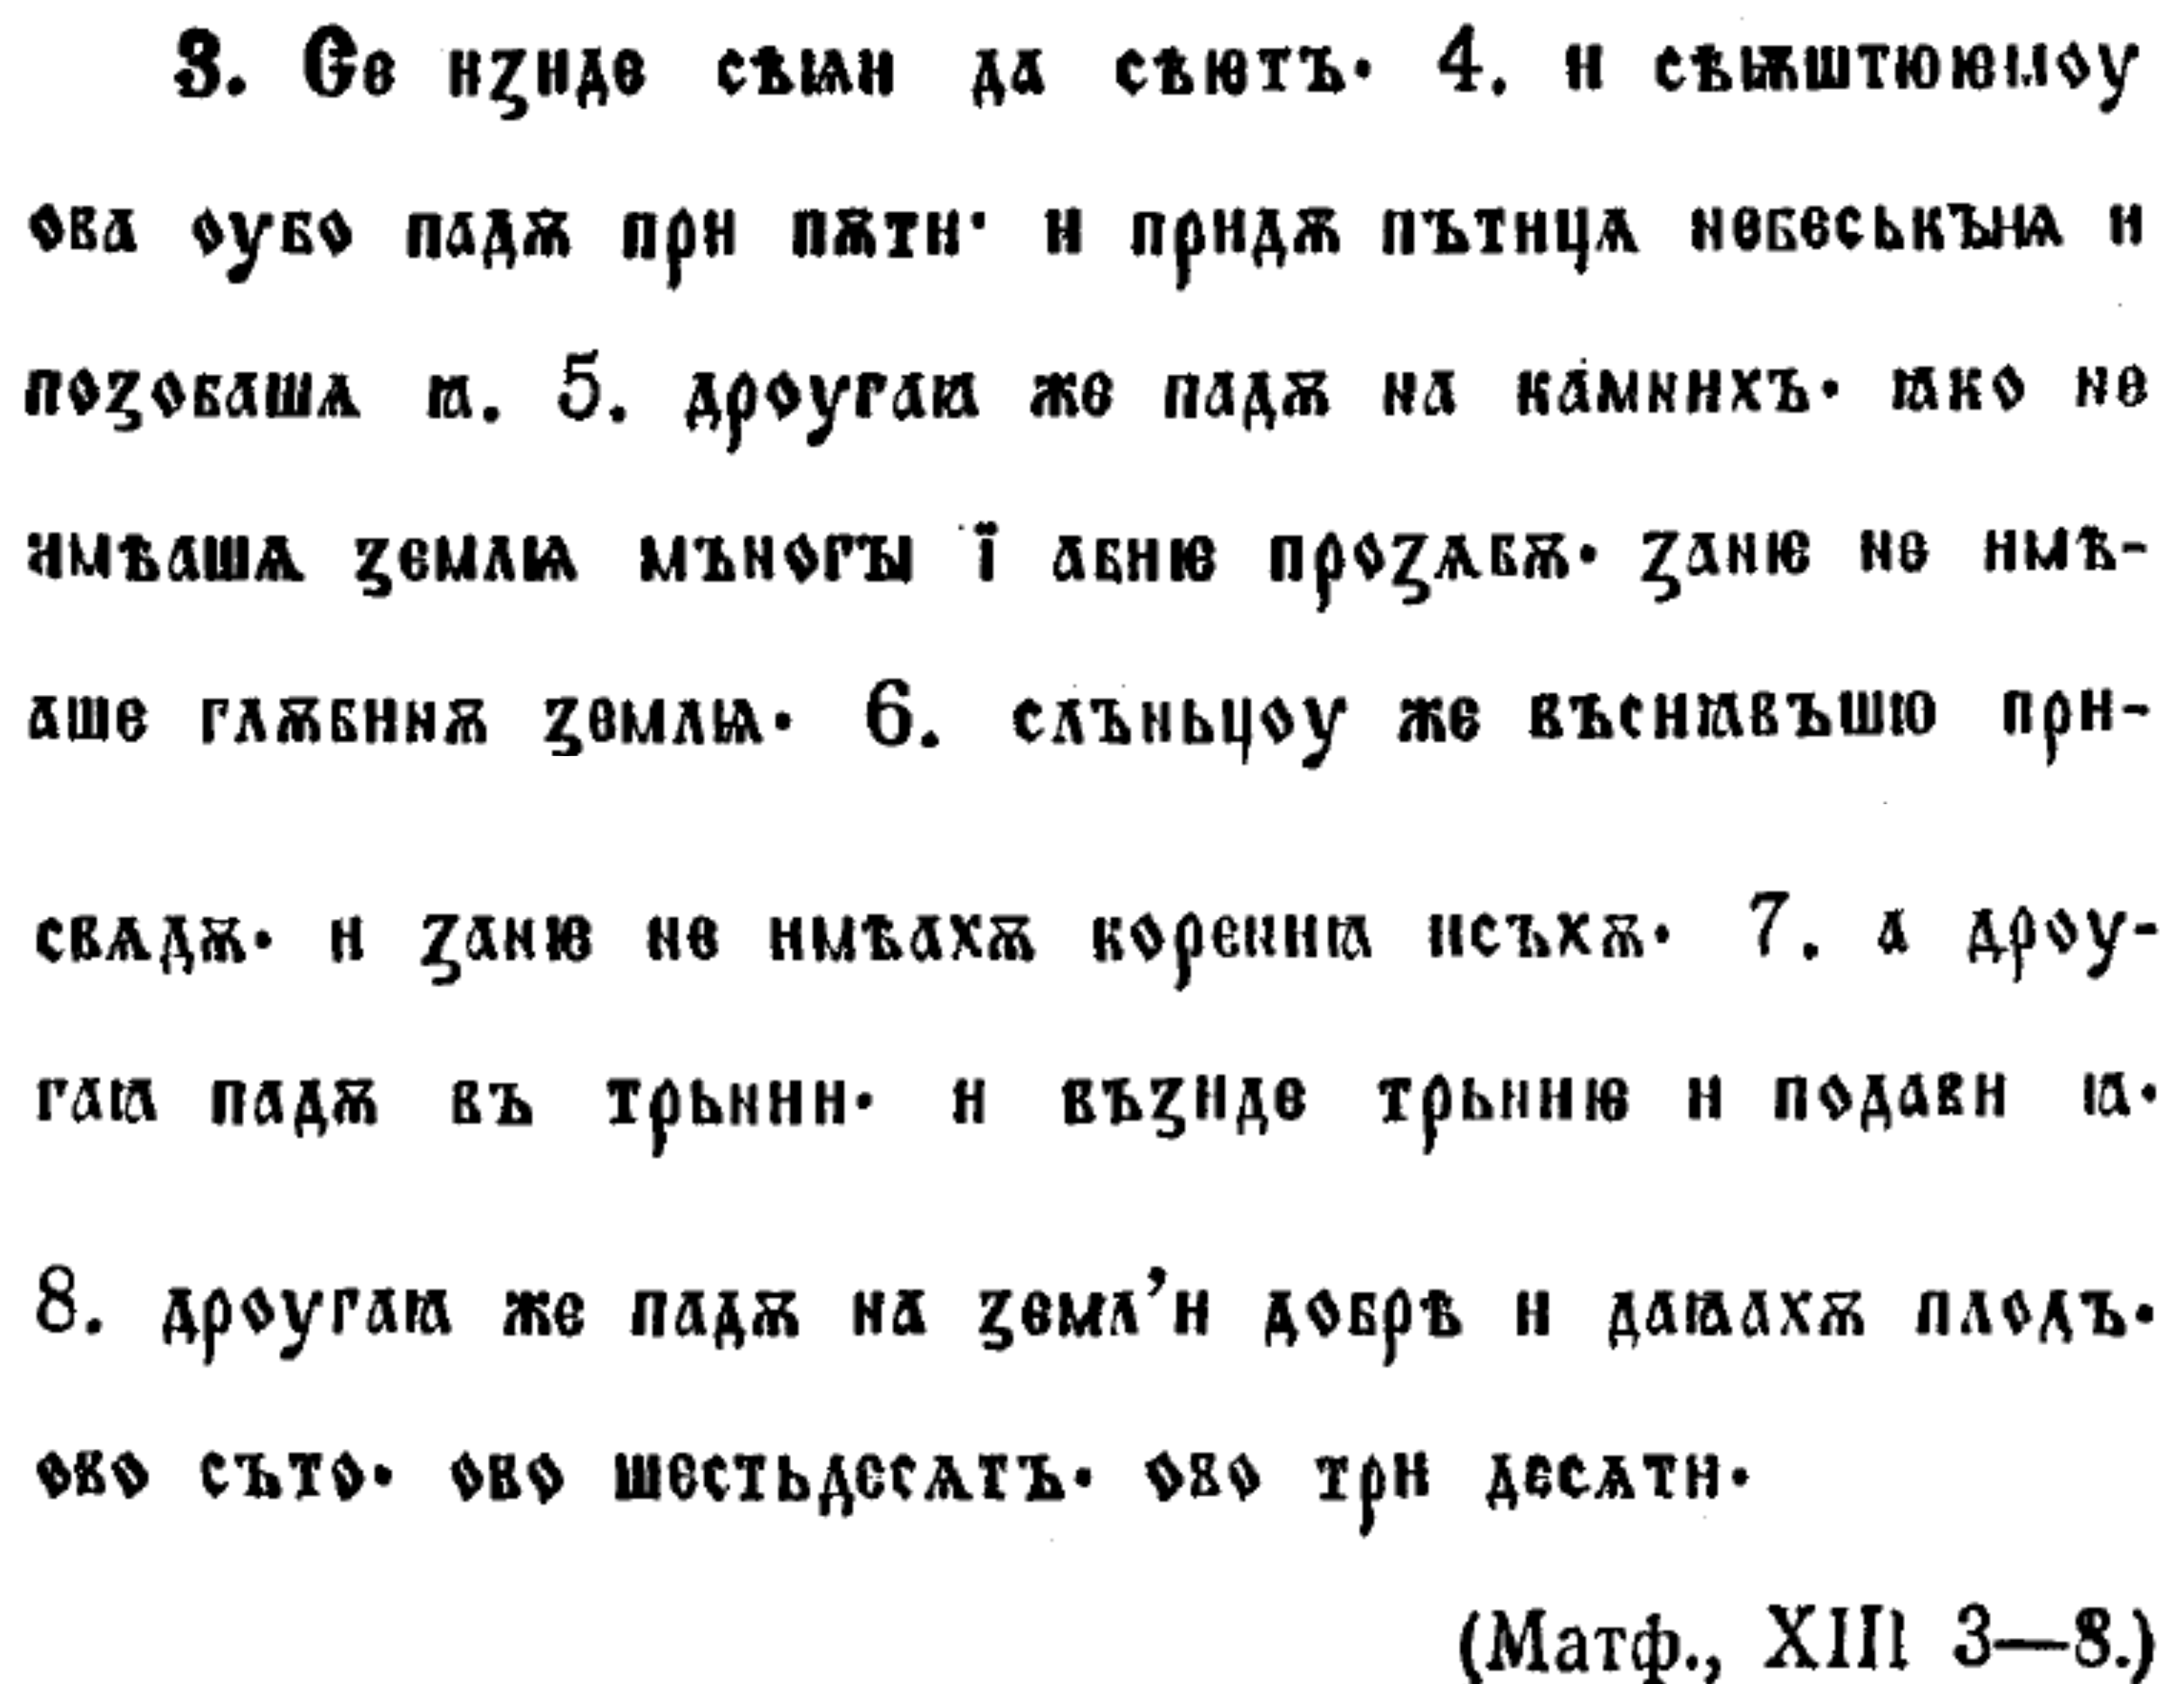
\includegraphics[width=0.93\textwidth]{ocs_sample_matthew13.png}

{\small\sffamily（Матф., XIII 3--8.）}
\end{center}

\sourcepage{120}{138}
\subsection*{译文}
3. 有一个撒种的出来撒种。4. 撒的时候，有落在路旁的，飞鸟来吃尽了。5、6. 有落在土浅石头地上的，土既不深，发苗就快，日头出来一晒，因为没有根，就枯干了。7. 有落在荆棘里的，荆棘长起来，把它挤住了。8. 又有落在好土里的，就结实，有一百倍的，有六十倍的，有三十倍的。（《新约・马太福音》第13章3--8句）

\subsection*{注释}
这段文字选自《马利亚福音书》（参看第63页），内容为《新约・马太福音》中撒种的比喻第3--8句。下面除说明词的形式和意义、进行必要的串讲之外，还附了俄译文和英译文各一种，以便对照。

\subsubsection*{第3句}
\begin{enumerate}[leftmargin=3em,label=\arabic*)]
\item \term{се}，语气词，用于故事开头，意在引起读（听）者的注意，可有“这时、那时、于是”等含义。俄译：\term{вот}。英译：\term{behold}。
\item \term{изиде}，动词，“出来”，不定式 \term{из-ити}。\term{изид-е}，不定过去时（非 s 型），单数第3人称，作谓语。俄译：\term{вышел}。英译：\term{went forth}。
\item \term{сѣяи}，“播（撒）种者”，阳性名词，句中主语。俄译：\term{сеятель}。英译：\term{a sower}。
\item \term{да сѣетъ}，“〔为了〕撒种”。动词虚拟式，这里由语气词 \term{да} 加动词 \term{сѣяти}（播种）的现在时单数第3人称形式构成，用来代替目的式或不定式。（比较：《马可福音》第4章第3句译为目的式：\term{се изиде ... сѣатъ}。）俄译：\term{[чтобы] сеять}。英译：\term{to sow}。
\end{enumerate}
1--4）俄译：\term{Вот вышел сеятель сеять}。英译：\term{Behold, a sower went forth to sow}。

\sourcepage{121}{139}
\subsubsection*{第4句}
\begin{enumerate}[leftmargin=3em,label=\arabic*),resume]
\item \term{и}，连接词，“和，并且，而”。俄译：\term{и}。英译本中译为 \term{and}。中译本未译出。
\item \term{сѣющю ему}，\term{сѣяти}（播种）的现在时主动形动词，长尾，单数，阳性，与格。此形式相当于俄语 \term{сеющему}。但在这里是“独立与格结构”，功能相当于时间状语从句：“当〔他〕撒种时”。俄译：\term{（и）когда он сеял}。英译：\term{And when he sowed}。
\item \term{ова}，“这些〔种子〕”，指示代词，变格同 \term{тъ}（那）：
\begin{center}
\begin{tabularx}{0.78\linewidth}{>{\bfseries}c *{3}{>{\centering\arraybackslash}X}}
\toprule
 & 阳性 & 中性 & 阴性\\
\midrule
单数 & овъ & ово & ова\\
复数 & ови & ова & овы\\
\bottomrule
\end{tabularx}
\end{center}
这里用的是中性复数主格，在句中作主语。由于是与下文相呼应使用的，所以可译为“有些（有的）……有些（有的）……”。俄译：\term{иное ... иное}。英译：\term{some ... some ...}。
\item \term{оубо}，语气词，“于是，结果，却，要知道”。俄译、英译皆略去。
\item \term{паде}，动词，“跌落”，不定式 \term{пасти < *pād-ti}。这里用的是不定过去时（非 s 型），复数第3人称，作 \term{ова} 的谓语。俄译：\term{（иное）упало}。英译：\term{fell}。
\item \term{при пути}，“〔落〕在路旁”。\term{при}，“在……近旁”，前置词，要求位格。阳性名词 \term{пѫть}（路）变格属 ī(ь) 类（\term{гость}）。词根中的鼻元音 \term{ѫ < on}，比较拉丁语 \term{pons}（属格 \term{pontis}，“桥”），法语 \term{pont [pɔ̃]}（桥）。俄译：\term{при дороге}。英译：\term{by the wayside}。
\end{enumerate}
7--10）俄译：\term{иное упало при дороге}。英译：\term{some seeds fell by the wayside}。
\begin{enumerate}[leftmargin=3em,label=\arabic*),resume]
\item \term{придѫ}，动词，“来”，不定式 \term{прити < при-ити}。这里用的是不定过去时（非 s 型），复数第3人称形式，相当于俄语的 \term{пришли}，作谓语。俄译本意译为 \term{налетели}（飞来）。英译：\term{came}。
\item \term{пътицѧ}，阴性名词 \term{пътица}（鸟）的复数主格，作主语。变格属 ā 类名词软变化；\term{ц} 在古斯拉夫语中是软音。俄译：\term{птицы}。英译：\term{the fowls}。
\item \term{небескъіѧ}，“天上的（鸟）”，由 \term{небо}（\term{небес-}，“天空”）派生的形容词，长尾，阴性，复数，主格，作定语。
\item \term{позобашѧ}，动词，“啄”，不定式 \term{позобати}。这里用的是不定过去时（s 型），复数第3人称，作谓语。俄译：\term{поклевали}。英译：\term{devoured them up}。
\end{enumerate}

\sourcepage{122}{140}
\begin{enumerate}[leftmargin=3em,label=\arabic*),resume]
\item \term{ѧ}，“这些，它们”，指示代词 \term{и} 的中性复数宾格形式（2.4.12），作直接宾语。
\end{enumerate}
11--15）俄译：\term{（и）налетели птицы и поклевали его}。英译：\term{（and）the fowls came and devoured them up}。

\subsubsection*{第5句}
\begin{enumerate}[leftmargin=3em,label=\arabic*),resume]
\item \term{другая}，“其他的，别的”，形容词 \term{другъ} 的长尾，中性，复数，主格。
\item \term{же}，“而”，表示转折的语气词，置于被强调的实词之后。俄、英译本中皆略去。
\item \term{на каменнихъ}，“〔落〕在多石的土地上”。\term{на}，“在……上”，前置词，表示处所时要求位格。\term{каменнихъ}（有的版本作 \term{каменистихъ}），中性名词 \term{камение}（多石的土壤）的复数位格。变格按 ŏ 类软变化。俄译：\term{на места каменистые}。英译：\term{upon stony places}。
\end{enumerate}
16--18）俄译：\term{иное упало на места каменистые}。英译：\term{some fell upon stony places}。
\begin{enumerate}[leftmargin=3em,label=\arabic*),resume]
\item \term{иже}，关系代词，在从句中作主语。
\item \term{не имѣашѧ}，动词，“（没）有”，不定式 \term{имѣти}。这里用的是未完成时复数第3人称；本应作 \term{имѣахѫ}，\term{-шѧ} 是在不定过去时影响下产生的新词尾。
\item \term{землѧ многы}，“许多泥土”，阴性单数属格；主格是 \term{землѧ}（泥土）、\term{многы}（许多的），变格属 ā 类阴性名词，前者为软变化，后者属硬变化（同 \term{жена}）。在句中作宾语。
\end{enumerate}
19--21）俄译：\term{... где не было много земли}。英译：\term{... where there had not much earth}。
\begin{enumerate}[leftmargin=3em,label=\arabic*),resume]
\item \term{абие}，“不久，很快”，副词。俄译：\term{скоро}。英译：\term{（and）forthwith}。
\item \term{прозѧбѫ}，动词，“发芽，出苗”，不定式 \term{прозѧб-нѫ-ти}。这里用的是不定过去时（非 s 型），复数第3人称，作谓语。后缀 \term{-нѫ-} 脱落（见第111页）。俄译：\term{взошло}。英译：\term{they sprung up}。
\item \term{зане}，“因为”，连接词。
\item \term{не имѣаше}，动词，“（没）有”，参看注释20。这里用的是未完成时单数第3人称。
\item \term{глѫбинѫ}，“深度”，阴性名词 \term{глѫбина} 的单数宾格，变格属 ā 类硬变化。
\end{enumerate}
24--26）俄译：\term{потому что земля была не глубока}。英译：\term{because they had no deepness of earth}。

\sourcepage{123}{141}
\subsubsection*{第6句}
\begin{enumerate}[leftmargin=3em,label=\arabic*),resume]
\item \term{слъньцю}（= \term{слъньцю}），中性名词 \term{слъньце}（太阳）的单数与格，属 ŏ 类软变化。
\item \term{въсиѧвъшю}，动词，“照耀”，不定式 \term{въсиѧти}。这里用的是过去时主动形动词，短尾，中性，单数，与格，同名词 \term{слъньцю}（太阳）一致。
\end{enumerate}
27--28）\term{слъньцю же въсиѧвъшю} 是“独立与格结构”（参看注释6），相当于时间状语从句：“当太阳照射时”。俄译：\term{когда же взошло солнце}。英译本：\term{and when the sun was up}。
\begin{enumerate}[leftmargin=3em,label=\arabic*),resume]
\item \term{присвѧдѫ}，动词，“晒蔫，萎缩”，不定式 \term{присвѧ-нѫ-ти}。这里用的是不定过去时（非 s 型），复数第3人称，作谓语。后缀 \term{-нѫ-} 脱落（见第111页）。俄译：\term{увяло}。英译处理为 \term{they were scorched}。
\item \term{корениѧ}，“根”，中性集合名词 \term{корение} 的属格，作宾语。变格属 ŏ 类软变化。俄译：\term{корня}。英译：\term{root}。
\item \term{исъхѫ}，动词，“干枯，枯死”，不定式 \term{исъх-нѫ-ти}。这里是不定过去时（非 s 型），复数第3人称，作谓语。后缀 \term{-нѫ-} 脱落（参看第111页）。俄译：\term{засохло}。英译：\term{they withered away}。
\end{enumerate}
30--31）俄译：\term{... и, как не имело корня, засохло}。英译本处理为：\term{... and because they had no root, they withered away}。

\subsubsection*{第7句}
\begin{enumerate}[leftmargin=3em,label=\arabic*),resume]
\item \term{въ трьнии}，“〔落〕入荆棘丛中”。\term{въ}，“进入”，前置词，这里要求位格。\term{трьнии}，中性集合名词 \term{трьние}（荆棘）的位格，变格属 ŏ 类软变化。
\end{enumerate}
俄译：\term{иное упало в терние}。英译：\term{And some fell among thorns}。
\begin{enumerate}[leftmargin=3em,label=\arabic*),resume]
\item \term{възиде}，动词，“上升，长出来”，不定式 \term{въз-ити}。这里用的是不定过去时（非 s 型），单数第3人称，作谓语。俄译：\term{выросло терние}。英译：\term{and the thorns sprung up}。
\item \term{подави}，动词，“压倒，挤死”，不定式 \term{подавити}。这里是不定过去时（s 型），单数第3人称，作谓语。俄译：\term{（и）заглушило его}。英译：\term{（and）choked them}。
\end{enumerate}

\sourcepage{124}{142}
\subsubsection*{第8句}
\begin{enumerate}[leftmargin=3em,label=\arabic*),resume]
\item \term{на земли добрѣ}，“〔落〕在好的泥土上”。\term{на}，见注释18。\term{земли}，阴性名词 \term{землѧ}（泥土）的单数位格，属 ā 类软变化。\term{добрѣ}，形容词 \term{добръ}（好的）的短尾，阴性单数位格，变格属 ā 类名词硬变化（同 \term{жена}）。
\end{enumerate}
俄译：\term{иное упало на добрую землю}。英译：\term{but other fell into good ground}。
\begin{enumerate}[leftmargin=3em,label=\arabic*),resume]
\item \term{дајаахѫ}，动词，“给，提供，带来”，不定式 \term{давати}。这里用的是未完成时，复数第3人称，作谓语；由后起的现在时词干（\term{даје-}）和后缀 \term{-аах-} 及词尾构成：\term{дај-аах-ѫ}。其他版本中可见到由不定式同干 \term{дад-} 构成的古形式：\term{дадѣахѫ < *dad-ěach-ę}。
\item \term{плодъ}，“果实”，阳性名词，属 ŏ 类硬变化（同 \term{рабъ}）。这里是单数宾格，作宾语。
\end{enumerate}
36--37）俄译：\term{（и）принесло плод}。英译：\term{（and）brought forth fruit}。
\begin{enumerate}[leftmargin=3em,label=\arabic*),resume]
\item \term{ово ... ово ... ово ...}，“有的……有的……有的……”，指示代词 \term{овъ} 的单数中性主格形式，参看注释7。
\item \term{съто}，“百”，变格同 ŏ 类中性名词硬变化（\term{село}）。这里是单数宾格。
\item \term{шесть десѧть}，“六十”，由 \term{шесть}（六）加 \term{десѧть}（十）的复数属格构成（见2.4.18）。
\item \term{три десѧти}，“三十”。后者是 \term{десѧть} 的复数主格（见2.4.18）。
\end{enumerate}
38--41）俄译：\term{одно во стократ, а другое в шестьдесят, иное же в тридцать}。英译：\term{some an hundredfold, some sixtyfold, some thirtyfold}。

\chaptercoverpage{第三章}{俄语}{ch03.jpg}
\chapter{俄语}

\section*{1. 引言}
\sourcepage{125}{143}
\phantomsection\addcontentsline{toc}{section}{1. 引言}
\origitem{3.1.1}
俄语（\term{русский язык}）是俄罗斯人的民族语言，也是苏联的官方语言。\footnote{校勘：把俄语笼统称为“苏联的官方语言”不够准确。苏联在其大部分存在时期没有由联盟宪法明确规定的单一“官方语言”；俄语长期事实上承担全联盟行政、教育和族际交往的主要共同语功能。直到 1990 年《苏联各民族语言法》才在联盟法律层面明确赋予俄语“苏联官方语言”（\term{официальный язык СССР}）的地位。正文依原印保留。}苏联境内的俄罗斯人超过 1.37 亿，占全国人口的 52.4\%（1979 年）；但以俄语为母语的人超过 1.4 亿，另有以它为第二母语、能自由使用的人 4,200 万。在国外，操俄语的人有 120 多万，分布在北美（主要是美国）和西欧等地区。

俄语属斯拉夫语族的东支，它的近亲语言是乌克兰语和白俄罗斯语。

\origitem{3.1.2}
东斯拉夫人在古希腊、拉丁史书中被称为“安特人”（\term{Ἄνται; Antes, Antae, Anti}），起初居住在德涅斯特河与第聂伯河之间。先后同他们为邻、有过长期接触的主要民族，在南方的有喀尔巴阡山麓操印欧语的色雷斯人，黑海北岸操伊朗语的西徐亚人和萨尔马特人，操印欧语的日耳曼（哥特）人以及操突厥语的阿瓦尔人和可萨人；北方的邻族是芬兰人和波罗的人（立陶宛人、拉脱维亚人、古普鲁士人）。据约尔丹内斯记载，4 世纪时东哥特国王维尼塔尔曾击败安特人的部落联盟，杀死大公博日及其儿子和部落首领 70 余人，将他们征服。自 6 世纪起，突厥游牧民族阿瓦尔人和可萨人也曾先后统治过某些东斯拉夫人部落。\footnote{哥特人的统治在斯拉夫语中留下了显著的痕迹，像 \term{меч}（剑）、\term{шлем}（盔）、\term{князь}（长官、大公）、\term{полк}（军队）等日耳曼借词便是从哥特语来的。}


自 2 世纪至 9 世纪，东斯拉夫人一直向四面八方迁徙和扩张：北至卢加河、沃尔霍夫河流域；东北抵达杰斯纳河、奥卡河、伏尔加河上游；东南至德涅斯特河、南布格河、第聂伯河下游与黑海北岸；向西推进到西布格河。不过，9--10 世纪时，由于受到突厥游牧民族佩彻涅格人的侵扰，一度离开黑海沿岸向北迁移，从而同南部斯拉夫人隔离。

\sourcepage{126}{144}
《往年纪事》中记述了 12 个东斯拉夫部落或部落联盟。\footnote{《往年纪事》（\term{Повесть временных лет}）是 12 世纪初由涅斯托尔（\term{Нестор}）在基辅编成，后世多把它加在编年史的开头，所以又称《编年序史》。书中所记部落分布情况主要是 9 世纪的。}最北面是伊尔门斯洛夫人（\term{ильменские словене}），定居在伊尔门湖、拉多加湖和沃尔霍夫河流域，该地区最古的城市是诺夫哥罗德。他们的南邻克里维奇人（\term{кривичи}）据有西德维纳河、伏尔加河与第聂伯河上游的广阔土地，那一带的早期城市是斯摩棱斯克、普斯科夫和波洛茨克。\footnote{拉脱维亚人的祖先曾长期与克里维奇人为邻。拉脱维亚语至今把俄罗斯人叫作 \term{krievs}。}居住在西德维纳河与普里皮亚季河之间的是德列戈维奇人（\term{дреговичи}“沼泽人”），其早期城市是图罗夫和平斯克。索日河（第聂伯河左岸支流）流域住有拉季米奇人（\term{радимичи}）。在顿河、奥卡河上游定居着维亚迪奇人（\term{вятичи}），其早期城市有梁赞等。\footnote{编年史中说，他们是 \term{Радим}（拉季姆）和 \term{Вятка}（维亚特卡）兄弟二人的后裔。}占据杰斯纳河、谢伊姆河与苏拉河一带的称为塞维里安人（\term{северяне}“北方人”），主要城市是切尔尼戈夫。位于第聂伯河右岸、普里皮亚季河以南的叫作德列夫利安人（\term{древляне}“森林人”）。在他们东南，定居于第聂伯河中游右岸（北起捷捷列夫河，南至罗斯河）的，是在东斯拉夫历史上起过重要作用的波利安人（\term{поляне}“平原人”）；波利安人土地上的历史名城基辅被誉为“俄罗斯众城之母”。居住在东南德涅斯特河流域的是乌利奇人（\term{уличи}）和蒂维尔人（\term{тиверцы}）。在西南的部落是杜列布人（\term{дулебы}）和白克罗地亚人（\term{белые хорваты}），前者定居于南布格河与西布格河之间，后者定居于喀尔巴阡山麓。


\sourcepage{127}{145}
公元 882 年，东斯拉夫人以奥列格大公为首建立了以基辅为首都的罗斯国，史称基辅罗斯（\term{Киевская Русь}）。988（或 989）年，弗拉基米尔大公受洗，奉基督教（拜占廷的东正教）为国教。\footnote{弗拉基米尔自 970 年起为诺夫哥罗德大公，980 年起为基辅大公，统治罗斯全境。}10 世纪末--11 世纪上半叶国势鼎盛，逐渐形成古俄罗斯部族。原先的部落名称在编年史中逐渐消失，而以所居住的地名代之。如斯洛夫人改称诺夫哥罗德人，维亚迪奇人改称梁赞人，波利安人改称基辅人，克里维奇人改称波洛茨克人，杜列布人改称沃伦人和布格人等等。12 世纪，出现封建割据局面，基辅罗斯解体，分裂为十多个互不相属的小公国：基辅、斯摩棱斯克、切尔尼戈夫、梁赞、诺夫哥罗德、罗斯托夫--苏兹达利等，内讧频仍，不能一致对敌，时常受到异族侵扰。13 世纪初，蒙古军队西侵，成吉思汗之孙拔都于 1240 年攻陷基辅，征服罗斯全境，以伏尔加河下游的萨莱为都建立钦察汗国，通过封建王公进行了 200 多年的统治（1243--1480 年），史称“蒙古--鞑靼桎梏时期”（\term{монголо-татарское иго}）。\footnote{汗帐殿金色，故又被俄罗斯人称为金帐汗国。}14 世纪前后，在蒙古人控制下的各公国互相争战，时有分合。在长期反对蒙古侵略者的斗争中，东北地区的罗斯托夫--苏兹达利一带，逐渐形成一个中央集权的莫斯科大公国。1480 年，伊凡三世（1462--1505）终于摆脱金帐汗国的桎梏，成为东北罗斯的领袖。伊凡四世（即伊凡雷帝，1530--1584）自 1547 年起称沙皇。这样，古代定居于北部和东北部的部落联盟（伊尔门斯洛夫人、克里维奇人、维亚迪奇人和部分塞维里安人）便融合为俄罗斯族。

另一方面，当 14 世纪东北罗斯处在金帐汗国势力之下时，西南罗斯，包括基辅、切尔尼戈夫、斯摩棱斯克、波洛茨克、弗拉基米尔--沃伦等公国，却为立陶宛侵占，而西部的加利西亚公国则为波兰征服。这样，古俄罗斯（东斯拉夫）部族便在 14--15 世纪分化为俄罗斯、乌克兰和白俄罗斯三支。

\sourcepage{128}{146}
东北罗斯从 14 世纪开始被邻国称为 \term{Великая Русь}（大罗斯），以区别于西南的 \term{Малая Русь}（小罗斯）和西部的 \term{Белая Русь}（白罗斯），但它的自称仍只是 \term{Русь}。15 世纪末--16 世纪初开始称 \term{Русия}（鲁西亚）和 \term{Росия}（罗西亚）。至 17 世纪中叶（1654 年）乌克兰左岸地区并入莫斯科国后，原东北罗斯才正式称 \term{Великая Росия}（大俄罗斯）。\term{Россия} 一词的写法（-сс-）始自 17 世纪末。


在外国史籍中，\term{Ros, Rosia} 可见于拜占廷皇帝君士坦丁七世（905--959）的《帝国行政论》（\term{De administrando imperio}，949）；他曾出访过罗斯国。\footnote{校勘：未见可靠史料证明君士坦丁七世本人曾出访罗斯。《帝国行政论》中关于罗斯交通路线、政治和礼俗的材料主要属于宫廷汇集的外交、地理和使节情报；将其叙述直接理解为作者亲历并不成立。}亦说 \term{Ros} 这个族称最早见于 6 世纪中叙利亚人著作中。

\term{Русь} 或 \term{Рос} 词源不详，至今没有公认的说法。较早的“诺曼起源说”认为，最初参与建国的军事首领留里克（\term{Рюрик}）等是来自斯堪的纳维亚但后来被同化的瓦兰人（\term{варяг < varęgъ}），即诺曼人，他们被斯拉夫人称为 \term{Rus}。据认为，\term{Rus} 源于芬兰语，芬兰人古时称波罗的海彼岸人为 \term{Ruotsi}（今义“瑞典”）。然而，俄国和苏联学者大都反对这种观点，认为 \term{Русь} 或 \term{рос} 最初可能是某个居住在第聂伯河支流罗斯河 \term{Рось（< Рьсь）} 的斯拉夫部族的名称。

\origitem{3.1.3}
东斯拉夫语（古俄语）约在 6 世纪脱离原始斯拉夫语，至 14--15 世纪分化为三个独立的语言——俄语、乌克兰语和白俄罗斯语。俄语是在罗斯托夫--苏兹达利（包括莫斯科）、诺夫哥罗德、普斯科夫、梁赞等地域方言基础上形成的。16 世纪中叶印刷术传入后，对俄语的统一起了推动作用。17--19 世纪形成俄罗斯民族语言。从普希金（\term{А. С. Пушкин}，1799--1837）时代开始形成以莫斯科方言为基础的现代俄罗斯标准语。对于标准语规范的形成，18--19 世纪的其他优秀作家，如莱蒙托夫（\term{М. Ю. Лермонтов}，1814--1841）、果戈理（\term{Н. В. Гоголь}，1809--1852）、屠格涅夫（\term{И. С. Тургенев}，1818--1883）、托尔斯泰（\term{Л. Н. Толстой}，1828--1910）、契诃夫（\term{А. П. Чехов}，1860--1904）等，也作出了很大贡献。

\origitem{3.1.4}

现存最早的古俄语文献有：《奥斯特罗米尔福音书》（\term{Остромирово евангелие}，1056--1057 年）、《特穆塔拉坎碑文》（\term{Надпись на Тмутараканском камне}，1068 年）、《俄罗斯法典》（\term{Русская правда}，1054 年汇编）、《往年纪事》（\term{Повесть временных лет}，12 世纪）、《伊戈尔王远征记》（\term{Слово о полку Игореве}，12 世纪）。后三个文献原本散失，现在只存有 13--14 世纪的传抄本。

\sourcepage{129}{147}
\sourcepage{130}{148}
如 2.1.2 节所说，俄语所使用的斯拉夫字母是 10 世纪末基辅罗斯接受基督教后，随着宗教文献（福音书、圣歌集、使徒行传、祈祷词等）从保加利亚传入的。\footnote{有些学者认为东斯拉夫人早在接受基督教以前已有了自己的文字。主要根据是：1）据《君士坦丁传》记载，公元 860 年，君士坦丁（基里尔）抵达科尔孙（\term{Корсунь = Херсонес}，克里木半岛西南端的一座古城），在那里发现了一部 \term{руськими（росьскими 或 рушкими）письменами}“用罗斯字母”写的福音书；2）据编年史记载，907 年，罗斯人曾同希腊人订过一些条约，既然是条约，总该是成文的；3）1949 年，在斯摩棱斯克以南的格尼奥兹多沃古冢群中发掘出的文物中，有 10 世纪初的陶坛，上有铭文（残存一个词）。然而这种意见没有得到公认，因为对上述论据有不同的解释。参看：\term{Иванов В. В. Историческая грамматика русского языка. М., 1983, с. 59；Бернштейн С. Б. Константин-Философ и Мефодий. М., 1984, с. 63 и сл.}}这些宗教书籍是从希腊语译成古斯拉夫语的。由于当时各支斯拉夫语可以互通，古斯拉夫语便成为一种各族斯拉夫人都能读懂的书面共同语。但它同古俄罗斯人的大众口语毕竟有一定的差别。后来，随着时间的推移距离渐大，书面语（标准语）便分化为两种形式：古斯拉夫语和用基里尔字母书写的古俄语。前者主要用于宗教书籍，虽然在传抄过程中必然搀入些古俄语成分，成为所谓的俄罗斯版本的古斯拉夫语，但在宗教界长期使用过程中一直保持着自己的基本特点，所以习惯上亦称教会斯拉夫语。至于古俄语，则用于世俗文献，如文学作品和各种文书（条约、契约、诉讼记录、遗嘱、书信等），前者多属书卷体性质，后者比较接近口语。但当时真正的大众口语尚未进入标准语。经过数百年的发展，古斯拉夫语词的使用范围日益缩小，以大众口语为基础的俄语用得越来越广泛，到近代形成以莫斯科口语为基础的标准语。不过，俄语毕竟吸收了许多古斯拉夫语成分。有些古斯拉夫词甚至取代了俄语固有词，如 \term{враг}（敌人）、\term{время}（时间）、\term{вождь}（领袖）、\term{единый}（统一的）等淘汰了古俄语的 \term{ворог, веремя, вожь, одиный} 等。另一些古斯拉夫词进入俄语后则与固有词并存，而在语义或语体（修辞色彩）上有所分工：\term{страна}（国家）—\term{сторона}（方向，方面），\term{глава}（首领）—\term{голова}（头），\term{одежда}（衣服）—\term{одёжа}（〈俗〉衣裳），\term{страж}（〈文语〉保卫者）—\term{сторож}（门卫，更夫）。比较：\term{Армия — верный страж завоеваний революции.}（军队是革命成果的忠实捍卫者。）；\term{Заводу требуется сторож.}（本厂招雇门卫。）（参看 1.3.7）


与俄语不同，现代乌克兰语和白俄罗斯语中则没有古斯拉夫语词（晚期从俄语借入的不算）。\footnote{校勘：这一说法过于绝对。乌克兰语和白俄罗斯语的书面传统同样长期受到教会斯拉夫语影响，词汇中存在不同层次的教会斯拉夫语成分；只是其数量、分布和在现代标准语中的文体功能与俄语不同。因而不宜概括为“没有古斯拉夫语词”。}如乌克兰语至今仍在使用 \term{ворог}（敌人）、\term{голова}（首领）、\term{одежа}（衣服）等古俄语固有词。

\section*{2. 字母与拼读}
\phantomsection\addcontentsline{toc}{section}{2. 字母与拼读}
\origitem{3.2.1}
俄语现在使用的是经过简化和改进的基里尔字母。1708 年，根据彼得大帝（1672--1725）的旨意，将宗教界用的笔划复杂的“斯拉夫字母”简化为易于书写的“民用字母”（\term{гражданский алфавит}），并废除了几个多余的字母。后来，这套字母又经过某些修改为一些其他斯拉夫国家所采用。18 世纪卡拉姆津（\term{Н. М. Карамзин}）所创造的字母 \term{ё} 于 1834 年正式列入字母表。\footnote{校勘：\term{ё} 并非卡拉姆津个人“创造”。1783 年叶卡捷琳娜・达什科娃已在俄国科学院会议上倡议用 \term{ё} 表示相应音值，卡拉姆津后来对其传播和文学使用起了重要作用。\term{ё} 进入俄语字母体系也是一个渐进过程，不能简单系于“1834 年正式列入”这一单一事件。}1917--1918 年，苏联政府又废除了四个多余的字母：\term{ѣ}（与 \term{е} 重复）、\term{ѳ}（与 \term{ф} 重复）、\term{і} 和 \term{ѵ}（与 \term{и} 重复）。\footnote{校勘：1917--1918 年正字法改革的法令明确废除的是 \term{ѣ, ѳ, і}，并取消词末硬音符号等旧写法；\term{ѵ}（ижица）在改革前已经极少使用，改革文件并未把它作为与前三字母同等的明确废除项目。现代资料常说它在改革中“事实上退出”字母表。}现在的字母表包括 33 个字母（见下页）：


\begin{center}\small
\begin{tabularx}{0.98\linewidth}{>{\bfseries}c >{\bfseries}c >{\centering\arraybackslash}p{1.8cm} >{\centering\arraybackslash}p{2.2cm} X}
\toprule
\sourcepage{131}{149}
次序 & 字母 & 名称 & 基本读音 & 例词\\
\midrule
1 & А а & а & a & ата́ка（冲锋），ва́за（花瓶）\\
2 & Б б & бэ & b & ба́ба（女人），быть（是）\\
3 & В в & вэ & v & вы（你们），трава́（青草）\\
4 & Г г & гэ & g & нога́（脚），гора́（山）\\
5 & Д д & дэ & d & дар（赠品），ду́мать（想）\\
6 & Е е & е & 'e; je & нет（不对），есть（吃）\\
7 & Ё ё & ё & 'o; jo & мёд（蜜），ёлка（圣诞树）\\
8 & Ж ж & жэ & ž = ʒ & жена́（妻子），мо́жно（可以）\\
9 & З з & зэ & z & за́втра（明天），сра́зу（立刻）\\
10 & И и & и & i & и́ли（或者），пить（喝）\\
11 & Й й & и краткое & j, i̯ & райо́н（区域），май（五月）\\
12 & К к & ка & k & рука́（手），кни́га（书）\\
13 & Л л & эл & l; lʲ & ла́мпа（灯），то́лько（仅、只）\\
14 & М м & эм & m & ма́ма（妈妈），там（那里）\\
15 & Н н & эн & n & нос（鼻子），сон（睡眠、梦）\\
16 & О о & о & o & но（但是），мо́да（时装）\\
17 & П п & пэ & p & па́па（爸爸），ша́пка（帽子）\\
18 & Р р & эр & r & рот（嘴），гора́（山）\\
19 & С с & эс & s & усы́（胡须），суд（法院）\\
20 & Т т & тэ & t & тот（那个），так（这样）\\
21 & У у & у & u & у́мный（聪明的），тут（这里）\\
\bottomrule
\end{tabularx}
\end{center}
\clearpage

\begin{center}\small
\sourcepage{132}{150}
\begin{tabularx}{0.98\linewidth}{>{\bfseries}c >{\bfseries}c >{\centering\arraybackslash}p{1.8cm} >{\centering\arraybackslash}p{2.2cm} X}
\toprule
次序 & 字母 & 名称 & 基本读音 & 例词\\
\midrule
22 & Ф ф & эф & f & факт（事实），ка́федра（讲台）\\
23 & Х х & ха & x & ха́та（农舍），мех（毛皮）\\
24 & Ц ц & цэ & ts & цех（车间），кита́ец（中国人）\\
25 & Ч ч & че & tʃ & челове́к（人），меч（剑）\\
26 & Ш ш & ша & ʃ & шар（球体），наш（我们的）\\
27 & Щ щ & ща & ɕː；或 ʃtʃ & щётка（刷子），плащ（披风）\\
28 & Ъ ъ & твёрдый знак & 分音符 & съесть（吃完），объём（容量）\\
29 & Ы ы & ы & ɨ & мы（我们），ты（你）\\
30 & Ь ь & мягкий знак & 表示前辅音软化 & конь（马），степь（草原）\\
31 & Э э & э & e & э́то（这个），поэ́т（诗人）\\
32 & Ю ю & ю & 'u; ju & лю́ди（人们），мо́ю（〔我〕洗）\\
33 & Я я & я & 'a; ja & мя́со（肉），я（我）\\
\bottomrule
\end{tabularx}
\end{center}



\origitem{3.2.2}
字母 \term{г}（4）表示后舌浊塞音 [g]，而不同于乌克兰语和白俄罗斯语（通常读擦音）。字母 \term{ё}（7）主要用于词典、教科书中，以及需要注明应读 [′o] 或 [jo] 时。例如 \term{всё}（中性）—\term{все}（复数），\term{узнаём}（未完成体）—\term{узна́ем}（完成体）。在其他情况下，\term{ё} 皆可以用 \term{е} 代替，而读音仍同 \term{ё}。比如 \term{её}（她的）也可写 \term{ее}，但仍读作 [jiˈjo]。\term{ё} 永远带重音（参看 3.3.7 之 4）。

\sourcepage{133}{151}
字母 \term{о}（16）在非重读音节中读音同 \term{а}。字母 \term{ф}（22）主要用于外来词，如 \term{фо́то}（照片）、\term{миф}（神话）、\term{ка́федра}（讲坛、主教职务、教研室）等。字母 \term{щ}（27）莫斯科读作长软音 [ɕː]，列宁格勒常读作音组 [ʃtʃ]，两种读法都合乎标准。

硬音符号 \term{ъ}（28）和软音符号 \term{ь}（30）现在已经有些名不副实了。\term{ъ} 前的辅音字母常可读软音：\term{съел}（吃了）可读 [sjel] 或 [sʲjel]；\term{ь} 前的辅音字母通常读软音，但 \term{ж, ш} 永远读硬音：\term{ложь}（谎言），\term{ружьё}（枪），\term{вошь}（虱子），\term{шью}（〔我〕缝）。\term{ъ, ь} 的共同功能是作“分音符”，即表示其前辅音与其后元音之间有个 [j]，比较：\term{сел}（坐下了）—\term{съел}（吃了）；\term{Коля}（男名）—\term{колья}（“尖桩”，复数）。

\origitem{3.2.3}
10 个元音字母按表音功能可分为两组：
\begin{center}
\begin{tabular}{c c c c c}
\toprule
\multicolumn{5}{c}{第一组：表示元音并通常提示前辅音为硬音}\\
а & э & о & у & ы\\
\midrule
\multicolumn{5}{c}{第二组：表示元音并通常提示前辅音为软音}\\
я & е & ё & ю & и\\
\bottomrule
\end{tabular}
\end{center}
（1）组字母除表示相应元音外，还表示其前辅音字母读硬音；（2）组字母除表示元音 \term{а, э, о, у, и} 外，还表示其前辅音字母读软音：\term{я = ʲa, е = ʲe, ё = ʲo, ю = ʲu, и = ʲi}。此外，\term{я, е, ё, ю} 在词首、元音字母后或 \term{ъ, ь} 后表示音组：\term{я = ja, е = je, ё = jo, ю = ju}。例：\term{я́ма}（坑），\term{есть}（吃），\term{ёлка}（圣诞树），\term{ю́бка}（裙子）；\term{моя́}（“我的”，阴性），\term{поесть}（吃一些），\term{моё}（“我的”，中性），\term{мою́}（“我的”，阴性宾格）；\term{объя́тие}（拥抱），\term{семья́}（家庭），\term{съел}（吃了），\term{ателье́}（艺术家的工作室），\term{объём}（容量），\term{ружьё}（枪），\term{адъюта́нт}（副官），\term{семью́}（“家庭”，宾格）。

绝大多数辅音字母（\term{б, в, г, д, з, к, л, м, н, п, р, с, т, ф, х}）既可表示硬音，又可表示软音：在 \term{а, э, о, у, ы} 前、辅音字母前或词末读硬音；在 \term{я, е, ё, ю, и} 前或 \term{ь} 前读软音。例如：\term{л} 在 \term{ла́мпа}（灯）、\term{жа́лко}（遗憾）、\term{пол}（地板）之类的词中读硬音；在 \term{для}（为了）、\term{лить}（斟、倒）、\term{то́лько}（只，仅）之类的词中读软音。


\section*{3. 语音}
\sourcepage{134}{152}
\phantomsection\addcontentsline{toc}{section}{3. 语音}

\origitem{3.3.1}
现代俄罗斯标准语中有 42 个音位：5 个元音，37 个辅音。

\begin{center}
\begin{tabular}{l c c c}
\toprule
 & 前元音 & 央元音 & 后元音\\
\midrule
高（闭）元音 & и & ы & у\\
中元音 & э &  & о\\
低（开）元音 &  & а & \\
\bottomrule
\end{tabular}
\end{center}

\begin{landscape}
\begin{center}
\begin{tabularx}{0.96\linewidth}{>{\bfseries}p{2.2cm} C C C C C C}
\toprule
发音方式 & 双唇音 & 唇齿音 & 齿音 & 齿龈音 & 中舌音 & 后舌音\\
\midrule
塞音 & п, б; п′, б′ &  & т, д; т′, д′ &  &  & к, г; к′, г′\\
擦音 &  & ф, в; ф′, в′ & с, з; с′, з′ & ш, ж; ш′:, ж′: &  & х; х′\\
塞擦音 &  &  & ц & ч &  & \\
擦音（近音） &  &  &  &  & й & \\
鼻音 & м; м′ &  & н; н′ &  &  & \\
边音 &  &  & л; л′ &  &  & \\
颤音 &  &  &  & р; р′ &  & \\
\bottomrule
\end{tabularx}
\end{center}
\end{landscape}


\sourcepage{135}{153}
\origitem{3.3.2}
由于 \term{ы} 只能用于硬辅音后，而在软辅音后和词首只能用 \term{и}，所以许多学者（特别是莫斯科学派）认为 \term{ы} 不是独立的音位，而只是音位 \term{и} 的变体。比较：\term{игра́ть}“玩耍、游戏”--\term{сыгра́ть}“完成体”、\term{отыгра́ть}“赢回、赌完”；\term{иска́ть}“寻找”--\term{разыска́ть}“找到”；\term{мил}“亲爱的（短尾）”--\term{мыл}“洗（过去时阳性）”。

\origitem{3.3.3}
俄语元音系统中最重要的规律是弱化，即元音在非重读音节中音长缩短，音值也程度不同地减弱。变化最大的是字母 \term{а, о, е, я} 所表示的读音。现在略举数例说明一下。

字母 \term{о} 在非重读音节中的读音与 \term{а} 相同。两者在词首或重音前第一音节中都读作 [a]： \term{абрико́с}“杏”、\term{тако́й}“这样的”、\term{откупи́ть}“赎回”、\term{гора́}“山”。在其他非重读音节中，无论位于重音前或重音后，一律读作音值含糊的中性元音： \term{каранда́ш}“铅笔”、\term{ко́мната}“房间”、\term{повида́ть}“看看”、\term{хорошо́}“好”、\term{зо́лото}“黄金”。\footnote{苏联学术界习惯上标作 [ъ]。}

字母 \term{я} 在非重读音节中的读音与 \term{е} 相同。两者在重音前第一音节中都读作 \term{и--е} 之间的音，在词首时有 [j]，例如： \term{леса́}“森林（复数）”、\term{еди́ный}“统一的”、\term{мясно́й}“肉的”、\term{язы́к}“语言”。在其他非重读音节中，除词尾有些特殊外，一律读作音值含糊的中性元音： \term{лесово́д}“林学家”、\term{едини́ца}“单位”、\term{вы́нес}“取出（过去时阳性）”、\term{мясники́}“肉商（复数）”、\term{языки́}“语言（复数）”、\term{по́няли}“明白（过去时复数）”。\footnote{苏联学术界习惯上标作 [ь]。}

\origitem{3.3.4}
辅音中成清浊对立的有：
\begin{center}
\begin{tabular}{l *{12}{c}}
\toprule
清 & п & п′ & ф & ф′ & т & т′ & с & с′ & ш & ш′: & к & к′\\
浊 & б & б′ & в & в′ & д & д′ & з & з′ & ж & ж′: & г & г′\\
\bottomrule
\end{tabular}
\end{center}
\sourcepage{136}{154}
其余辅音不成对：\term{л, л′, м, м′, н, н′, р, р′, й} 九个响音没有相应清音位；\term{х, х′, ц, ч} 四个清音没有相应浊音位。

像大多数斯拉夫语一样，俄语的浊音（不包括响音）在词末或清音前要清化，亦即同相应的清音交替。例如： \term{хлеб, голубь, голов, кровь, рог, сад, лошадь, раз, грязь, муж, дождь} 等词，以及 \term{оши́бка, все, но́гти, ре́дко, ре́дька, но́жка, ре́зко} 等辅音连缀为例。

另一方面，清音在（\term{в, в′} 以外的）浊音前要发生浊化，即同相应的浊音交替。例如： \term{сде́лать}“做（完成体）”、\term{про́сьба}“请求”、\term{отбро́сить}“扔掉”、\term{молотьба́}“打谷、打场”、\term{профделега́т}“工会代表”为例。清音在 \term{в, в′} 前仍读清音，如 \term{твой}“你的”、\term{свет}“光、世界”；在响音前也不浊化。


\origitem{3.3.5}
辅音中成硬软对立的有 15 对：
\begin{center}
\begin{tabular}{l *{15}{c}}
\toprule
硬 & п & б & ф & в & т & д & к & г & х & с & з & м & н & л & р\\
软 & п′ & б′ & ф′ & в′ & т′ & д′ & к′ & г′ & х′ & с′ & з′ & м′ & н′ & л′ & р′\\
\bottomrule
\end{tabular}
\end{center}
其余辅音不成对：\term{ж, ш, ц} 永远是硬音，没有相应软音位；\term{ч, й, ж′:, ш′:} 永远是软音，没有相应硬音位。\term{ж} 和 \term{ж′:}、\term{ш} 和 \term{ш′:} 之所以不相对应，是因为除去硬软不同之外，还有长短的区别。

俄语辅音的硬软对立系统（共 15 对），是现代各斯拉夫语中最完整的。辅音软化（硬辅音同软辅音交替）的规律远没有清浊同化那么严整。在现代俄语中，硬辅音被其后软辅音同化为软音的现象在逐渐减少，标准音中必须软化的例子已经不多了。例如：\term{степь}“草原”、\term{здесь}“这里”、\term{кость}“骨头”、\term{винтик}“螺丝钉”、\term{песня}“歌”、\term{вонзить}“刺入”。


\sourcepage{137}{155}
\origitem{3.3.6}
俄语的音节结构多种多样，开音节与闭音节同样常见，同一音节中允许辅音连缀。例如 \term{го-ло-ва́}“头”、\term{тра-ва́}“青草”、\term{о-кно́}“窗户”都是开音节；\term{квар-та́л}“街区”、\term{вой-на́}“战争”的词首音节，以及 \term{пе-со́к}“沙”、\term{го́-род}“城市”的词末音节都是闭音节。词中可有二至四个辅音连缀，如 \term{блеск}“闪光”、\term{стра-на́}“国家”、\term{ми-ни́стр}“部长”、\term{встре́-ча}“会见”、\term{вздра́-ги-вать}“发抖”。

词重音属混合型，重读元音既强又长，兼有力重音与长度重音的双重特征。从位置上看，重音是自由的，即在不同的词中可能落在不同的音节上，比较： \term{зо́лото, доро́га, хорошо́, сковорода́, достопримеча́тельность}。词发生形态变化时重音还可能移动，如 \term{рука́--ру́ку--ру́ки}，\term{нога́--но́гу--но́ги}。

由于非重读元音要弱化，而重音又是自由的、可移动的，因此同一个词的读音有时变化很大。比较： \term{голова́}（单数主格）、\term{го́лову}（单数宾格）、\term{голо́в}（复数属格）。不仅如此，在某些前置词短语（语音词）中，重音还可以从实词转移到前置词上。比较： \term{нога́--за́ ногу}，\term{голова́--на́ голову}，\term{бе́рег--на́ берег}。除词典、教科书等外，书面上一律不标重音，这给外国人的学习造成很大困难。

\origitem{3.3.7}
从历史演变的角度看，现代俄语的主要语音特征可以概括如下：
\begin{enumerate}[leftmargin=3em,label=\arabic*)]
\item 古代的鼻元音 \term{ǫ, ę} 分别演变为 \term{у, я (а)}：\term{dǫbъ > дуб}（橡树），\term{mǫžь > муж}（丈夫），\term{pętь > пять}（五），\term{sěmę > семя}（种子）。
\item 古代的短弱元音 \term{ъ, ь} 在弱位上消失，在强位上分别演变为 \term{о, е}：\term{sъnъ > сон}（睡眠，梦），\term{mъxъ > мох}（苔藓），\term{dьnь > день}（天，日），\term{pьsъ > пес > пёс}（狗）。
\item 古代的 \term{ě (ѣ)} 演变为 \term{е}：\term{lěsъ > лес}（森林），\term{město > ме́сто}（地方）。

\sourcepage{138}{156}
\item 古代的 \term{е}（包括 \term{е < ь}，但不包括 \term{е < ě}）在重读音节中硬辅音之前时演变为 \term{ё}：\term{ledъ > лёд}（冰），\term{neslъ > нёс}（“携带”，过去时阳性），\term{pьsъ > pes > пёс}（狗），\term{ženy > жёны}（“妻子”，主复）。比较：单主 \term{žena > жена́}，形容词 \term{жена́тый}“有妻子的”，动词 \term{жени́ть}（使结婚）。\footnote{参看乌克兰语（4.3.8 之 6）和波兰语（12.3.6 之 5）。}

试再比较：俄语固有词 \term{нёбо}（上腭），\term{падёж}（牲畜的死亡）--古斯借词 \term{не́бо}（天空），\term{паде́ж}（语法上的格）。
\item 古代的 \term{i} 和 \term{y (ы)} 虽有合流的趋势（3.3.2），但至今仍保留着明显的区别，因而时常引起学术界的争论：现在究竟是两个音位还是一个音位。
\item “а 口音”（\term{о} 在非重读音节中读作 \term{а}）；非重读元音的显著弱化。
\item 有全元音音组：\term{го́род}（城市），\term{бе́рег}（岸），\term{ко́лос}（穗），\term{молоко́}（奶）（1.3.7）。
\item 古俄语时期的 \term{ръ, рь, лъ, ль} 在非重读的开音节中变为 \term{ро, ло}：\term{krъvavъ(jь) > крова́вый}（流血的），\term{krъšiti > кроши́ть}（弄碎），\term{glъtati > глота́ть}（吞咽）。
\item \term{j} 前的紧弱元音（1.5.5）在强位上分别变为全值元音 \term{о, е}，在弱位上消失，也就是说，演变结果同短弱元音 \term{ъ, ь} 一样：\term{mŷjǫ > мо́ю}（〔我〕洗），\term{krŷjǫ > кро́ю}（〔我〕覆盖），\term{šija > ше́я}（脖子），\term{bîjь > бей}（“打”，命令式）；比较：\term{bьjǫ > бью}（〔我〕打），\term{šьjǫ > шью}（〔我〕缝）。
\item \term{kv(ě) > цве-，gv(ě) > зве-}：\term{květъ > цвет}（颜色，花朵），\term{gvězda > звезда́}（星）。
\item 辅音的硬软对立系统（共 15 对），在现代各斯拉夫语中是最发达的；辅音在 \term{и, е} 前软化（\term{диво}“奇事”，\term{несу}“〔我〕携带”）。
\sourcepage{139}{157}
\item 古代软音 \term{ж, ш, ц} 硬化：\term{жест}（手势）= \term{жэст}，\term{жёлтый}（黄色的）= \term{жолтый}，\term{жить}（生活）= \term{жыть}，\term{жюри}（裁判员）= \term{жури}，\term{ложь}（谎言）= \term{лож}，\term{ружьё}（枪）= \term{ружйо}；\term{шест}（竿）= \term{шэст}，\term{шёл}（“走”，过去时阳性）= \term{шол}，\term{шить}（缝）= \term{шыть}，\term{парашют}（降落伞）= \term{парашут}，\term{пишешь}（〔你〕写）= \term{пишэш}，\term{шью}（〔我〕缝）= \term{шйу}；\term{цель}（目的）= \term{цэль}，\term{цирк}（杂技团）= \term{цырк}。

\item “唇音 + \term{j}”有插入音 \term{л′}：\term{kupjǫ > куплю́}（〔我〕买），\term{l'ubjǫ > люблю́}（〔我〕爱），\term{zemja > земля́}（土地）。
\item \term{dj > ж；tj, ktj > ч}：\term{medja > межа́}（地界），\term{odědja > odeža > одёжа}（衣裳〈俗〉；古斯借词 \term{оде́жда}“衣服”）；\term{světja > свеча́}（“蜡烛”；古斯 \term{свѣшта}）。比较：\term{урожа́й}（收成，收获）--古斯借词 \term{рожде́ние}（降生），\term{горя́чий}（滚热的）--带古斯后缀的 \term{горя́щий}（燃烧着的）。
\item 形容词、代词的单数阳、中性属格词尾 \term{-ого, -его} 中的 \term{г [g]} 变为 [v]：\term{но́вого}（新的），\term{си́него}（蓝色的），\term{его́}（他的）。（参看第 152 页脚注 4）
\item 词首的 \term{je > o}：\term{jedinъ > оди́н}（一），\term{jezero > о́зеро}（湖），\term{jesenь > о́сень}（秋天），\term{jelenь > оле́нь}（鹿）。
\item 原始斯拉夫语时期的成节流音 \term{l, r}（\term{ъl, ьl > ол；ъr > ор；ьr > ер}）：\term{dъlgъ > долг}（债务），\term{mъlčěti > молча́ть}（沉默），\term{tъrgъ > торг}（交易），\term{pьrvъ(jь) > пе́рвый}（第一）。
\end{enumerate}

\section*{4. 语法}
\phantomsection\addcontentsline{toc}{section}{4. 语法}
\subsection*{а) 名词}
\phantomsection\addcontentsline{toc}{subsection}{а) 名词}
\origitem{3.4.1}
\sourcepage{140}{158}
俄语的名词有性、数、格、动物--非动物的语法范畴。名词分别属于阳性、阴性和中性。绝大多数的名词有单数和复数两种形式；古代的双数范畴已经消失，只剩下一些遗迹。格有六个：主格、属格、与格、宾格、工具格和位格（今通常称前置格）。古代的呼格形式几乎荡然无存，残余形式屈指可数： \term{боже!}“天哪”（源于 \term{бог}“神、上帝”）和 \term{господи!}“上帝啊”（源于 \term{господь}）；这两个词形如今只作感叹词用了。呼格在其他东斯拉夫语中则基本上保留下来（4.4.1；5.4.1）。

部分变格形式可以反映动物名词与非动物名词的区别：前者的宾格形式同属格，后者的宾格形式同主格。名词变格法分为三种主要类型，其中第 I、II 变格法又各有硬变化和软变化之分。


\origitem{3.4.2}
第 I 变格法（$<$ 古 \term{ŏ} 类变格）包括绝大多数阳性名词和中性名词：阳性的以辅音结尾（零词尾），如 \term{стол, нож, студе́нт, рабо́тник, това́рищ, конь, учи́тель, слова́рь, край, геро́й}；中性的以 \term{-о, -е} 结尾，如 \term{село́, ме́сто, мо́ре, по́ле, про́звище}。词干以硬辅音结尾的属硬变化，以软辅音结尾的属软变化。阳性和中性名词的区别主要在于主、宾格（单、复数）的词尾。

\begin{landscape}
\begin{center}
\begin{tabularx}{0.98\linewidth}{>{\bfseries}c >{\bfseries}c C C C C C C}
\toprule
数 & 格 & стол & студе́нт & ме́сто & конь & край & мо́ре\\
\midrule
单 & 主 & стол & студе́нт & ме́сто & конь & край & мо́ре\\
单 & 属 & стола́ & студе́нта & ме́ста & коня́ & кра́я & мо́ря\\
单 & 与 & столу́ & студе́нту & ме́сту & коню́ & кра́ю & мо́рю\\
单 & 宾 & 同主格 & 同属格 & 同主格 & 同主/属格 & 同主格 & 同主格\\
单 & 工 & столо́м & студе́нтом & ме́стом & конём & кра́ем & мо́рем\\
单 & 位 & столе́ & студе́нте & ме́сте & коне́ & кра́е & мо́ре\\
\midrule
复 & 主 & столы́ & студе́нты & места́ & ко́ни & края́ & моря́\\
复 & 属 & столо́в & студе́нтов & мест & коне́й & краёв & море́й\\
复 & 与 & стола́м & студе́нтам & места́м & коня́м & края́м & моря́м\\
复 & 宾 & 同主/属格 & 同主/属格 & 同主格 & 同主/属格 & 同主格 & 同主格\\
复 & 工 & стола́ми & студе́нтами & места́ми & коня́ми & края́ми & моря́ми\\
\sourcepage{141}{159}
复 & 位 & стола́х & студе́нтах & места́х & коня́х & края́х & моря́х\\
\bottomrule
\end{tabularx}
\end{center}
\end{landscape}


单数属格词尾是 \term{-а, -я}。

单数与格词尾是 \term{-у, -ю}。宾格无论单数还是复数，动物名词同属格，非动物名词同主格。比较：\term{Я ви́жу стол/столы́.}“我看见一张/许多桌子。”--\term{Я ви́жу студе́нта/студе́нтов.}“我看见一个/许多大学生。”

单数工具格词尾是 \term{-ом, -ем, -ём}（带重音）。

单数位格词尾，不分硬软变化，都是 \term{-е}。

某些阳性名词的单数属格，除 \term{-а, -я} 外，还可有词尾 \term{-у, -ю}，专门用来表示部分意义：\term{мёд--нет мёда--ло́жка мёду}“蜜--没有蜜--一勺蜜”，\term{чай--нет ча́я--стака́н ча́ю}“茶--没有茶--一杯茶”。某些阳性名词的单数位格，除 \term{-е} 外，还可有重读词尾 \term{-у, -ю}，专门用来表示处所意义：\term{лес--о ле́се--в лесу́}，\term{сад--о са́де--в саду́}，\term{край--о кра́е--в краю́}。属格词尾和位格（前置格）词尾 \term{-у, -ю} 都源于古 \term{ŭ} 类（\term{сынъ}）变格（2.4.5）。

复数主格的词尾因性而异：阳性名词是 \term{-ы, -и}，中性名词是 \term{-а, -я}。不过，有少数阳性名词的复数主格词尾是 \term{-а, -я}：\term{глаз--глаза́, бе́рег--берега́, рука́в--рукава́, дом--дома́, лес--леса́, го́род--города́, край--края́, учи́тель--учителя́}。词尾 \term{-а, -я} 最初是在古代双数主--宾格形式（2.4.4）影响下产生的。

值得一提的是，词干末尾的后舌音，在复数主格词尾 \term{-и} 前不发生 \term{г:з, к:ц, х:с} 的交替（第二次软化，1.4.3）。例如：\term{поро́г--поро́ги, рабо́тник--рабо́тники, волк--во́лки, страх--стра́хи}。

\sourcepage{142}{160}
复数属格词尾较复杂，主要有 \term{-ов, -ев, -ёв, -ей} 和零词尾，如 \term{столо́в, геро́ев, краёв, коне́й, море́й, ноже́й, това́рищей, мест}。零词尾通常限于中性名词硬变化，但也见于少数阳性名词，如 \term{пять челове́к, пять солда́т, нет глаз}。


复数与格为 \term{-ам, -ям}，工具格为 \term{-ами, -ями}，位格为 \term{-ах, -ях}。这三种词尾是在古代 \term{ā} 类变格（2.4.3）的类推作用下产生的。

少数名词有隐现元音 \term{о, е}：\term{сон--сна, сну；день--дня, дню；оте́ц--отца́, отцу́；окно́--о́кон}（参看 1.5.4）。中性名词 \term{о́ко}“眼睛（旧）”、\term{у́хо}“耳朵”单数变格规则，复数变化则保存古代双数形式的遗迹：
\begin{center}
\begin{tabular}{>{\bfseries}c c c}
\toprule
格 & о́ко & у́хо\\
\midrule
主 & о́чи & у́ши\\
属 & оче́й & уше́й\\
与 & оча́м & уша́м\\
宾 & о́чи & у́ши\\
工 & оча́ми & уша́ми\\
位 & оча́х & уша́х\\
\bottomrule
\end{tabular}
\end{center}

\origitem{3.4.3}
第 II 变格法（$<$ 古 \term{ā} 类变格）包括所有以 \term{-а, -я} 结尾的名词；其中绝大多数是阴性的，如 \term{жена́, же́нщина, сестра́, рабо́тница, кни́га, нога́, рука́, земля́, статья́, свинья́, семья́}。极少数名词是阳性的，如 \term{мужчи́на, воево́да, слуга́, ста́роста, де́душка, ю́ноша, дя́дя, судья́}。词干以硬辅音结尾的属硬变化，以软辅音结尾的属软变化。

单数属格词尾是 \term{-ы, -и}。\term{-и} 除用于软变化外，还用于 \term{г, к, х, ж, ш} 之后，如 \term{кни́га--кни́ги, рука́--руки́, му́ха--му́хи, ко́жа--ко́жи, гру́ша--гру́ши}。

单数与格和位格的词尾相同，一律是 \term{-е}。


\begin{landscape}
\begin{center}
\begin{tabularx}{0.98\linewidth}{>{\bfseries}c >{\bfseries}c C C C C C C}
\toprule
\sourcepage{143}{161}
数 & 格 & сестра́ & рабо́тница & кни́га & дя́дя & земля́ & семья́\\
\midrule
单 & 主 & сестра́ & рабо́тница & кни́га & дя́дя & земля́ & семья́\\
单 & 属 & сестры́ & рабо́тницы & кни́ги & дя́ди & земли́ & семьи́\\
单 & 与 & сестре́ & рабо́тнице & кни́ге & дя́де & земле́ & семье́\\
单 & 宾 & сестру́ & рабо́тницу & кни́гу & дя́дю & зе́млю & семью́\\
单 & 工 & сестро́й (-о́ю) & рабо́тницей (-ею) & кни́гой (-ою) & дя́дей (-ею) & землёй (-ёю) & семьёй (-ёю)\\
单 & 位 & сестре́ & рабо́тнице & кни́ге & дя́де & земле́ & семье́\\
\midrule
复 & 主 & сёстры & рабо́тницы & кни́ги & дя́ди & зе́мли & се́мьи\\
复 & 属 & сестёр & рабо́тниц & книг & дяде́й & земе́ль & семе́й\\
复 & 与 & сёстрам & рабо́тницам & кни́гам & дя́дям & зе́млям & се́мьям\\
复 & 宾 & 同主/属格 & 同主/属格 & 同主/属格 & 同主/属格 & 同主/属格 & 同主/属格\\
复 & 工 & сёстрами & рабо́тницами & кни́гами & дя́дями & зе́млями & се́мьями\\
复 & 位 & сёстрах & рабо́тницах & кни́гах & дя́дях & зе́млях & се́мьях\\
\bottomrule
\end{tabularx}
\end{center}
\end{landscape}


\sourcepage{144}{162}
词尾 \term{-е} 前的后舌音（即词干的尾辅音）不发生 \term{г:з, к:ц, х:с} 交替（第二次软化，见 1.4.3）；这一点与乌克兰语（4.4.2）、白俄罗斯语（5.4.3）不同。比较 \term{рука́}（手）的单数与格、位格：俄 \term{руке́}，乌 \term{руці́}，白 \term{руцэ́}。

单数宾格有自己特殊的词尾 \term{-у, -ю}，从不与主格或属格相同，也就是说，没有动物名词与非动物名词之分。单数工具格词尾为 \term{-ой, -ей, -ёй}（带重音），书面语中有时用 \term{-ою, -ею, -ёю}。

复数主格词尾为 \term{-ы, -и}，词尾前的后舌音 \term{г, к, х} 不再发生第二次软化遗留的交替。复数属格为零词尾或 \term{-ей}；少数零词尾形式中可出现隐现元音 \term{о, е, ё}：\term{ска́зка--ска́зок, земля́--земе́ль, сестра́--сестёр}。复数宾格有动物/非动物区别：动物名词同属格（如 \term{сестёр, рабо́тниц, дяде́й}），非动物名词同主格（如 \term{кни́ги, зе́мли, се́мьи}）。复数与格、工具格、位格分别为 \term{-ам/-ям, -ами/-ями, -ах/-ях}。

\origitem{3.4.4}
属于第 III 变格法（$<$ 古 \term{ī} 类变格）的是少数阴性名词，拼写上的特征是末尾都有 \term{-ь}：\term{ло́шадь, ра́дость, ночь, печь, кровь, любо́вь, соль, тень, кость, речь}。这些名词的单数主格都是零词尾，词干尾辅音大都是软的，只有极少数是硬的： \term{рожь, мышь}。嘘音 \term{ж, ш} 在古代也是软的，但后来硬化了，现在的写法已不反映实际发音（3.2.1），拼写时加 \term{-ь} 只表示这些名词是阴性的，属第 III 变格法。比较第 I 变格法中的阳性名词 \term{нож, пляж, слова́рь, вождь} 。第 III 变格法没有硬变化与软变化的区别。


\begin{center}
\begin{tabular}{>{\bfseries}c c c c c}
\toprule
格 & мышь（单） & ра́дость（单） & мышь（复） & ра́дость（复）\\
\midrule
\sourcepage{145}{163}
主 & мышь & ра́дость & мы́ши & ра́дости\\
属 & мы́ши & ра́дости & мыше́й & ра́достей\\
与 & мы́ши & ра́дости & мыша́м & ра́достям\\
宾 & 同主格 & 同主格 & 同属格 & 同主格\\
工 & мы́шью & ра́достью & мыша́ми & ра́достями\\
位 & мы́ши & ра́дости & мыша́х & ра́достях\\
\bottomrule
\end{tabular}
\end{center}

单数没有动物与非动物的区别，宾格都同主格；复数则有区别：动物名词宾格同属格，非动物名词宾格同主格。单数属格、与格和位格词尾相同，都是 \term{-и}，工具格为 \term{-ью}。复数主格词尾为 \term{-и}，属格为 \term{-ей}，与格、工具格、位格词尾与第 II 变格法相同，分别为 \term{-ам/-ям, -ами/-ями, -ах/-ях}。


\subsection*{б) 形容词}
\phantomsection\addcontentsline{toc}{subsection}{б) 形容词}
\origitem{3.4.5}
形容词有性、数、格的变化。词干以硬辅音结尾、单数阳性主格词尾是 \term{-ый, -ой} 的属硬变化，如 \term{но́вый}（新的）、\term{до́брый}（善良的）、\term{весёлый}（快活的）、\term{молодо́й}（年轻的）、\term{дорого́й}（亲爱的）；词干以软辅音结尾、单数阳性主格词尾是 \term{-ий} 的属软变化，如 \term{си́ний}（蓝色的）、\term{ле́тний}（夏季的）、\term{дома́шний}（家庭的）。词干以 \term{г, к, х, ж, ш, ч, щ, ц} 结尾、单数阳性主格词尾是 \term{-ий} 或 \term{-ой} 的，如 \term{стро́гий}（严厉的）、\term{вели́кий}（伟大的）、\term{ти́хий}（安静的）、\term{плохо́й}（坏的）、\term{све́жий}（新鲜的）、\term{хоро́ший}（好的）、\term{большо́й}（大的）、\term{горя́чий}（滚烫的、热的）等，变格时有某些特殊性，有时被视为混合变化。

形容词的单数形式有阳、中、阴性的区别，复数不分性；在这一点上所有东斯拉夫语是一致的。下面只举典型的硬、软变化为例。

\begin{landscape}

\begin{center}
\sourcepage{146}{164}
\begin{tabularx}{0.98\linewidth}{>{\bfseries}c >{\bfseries}c C C C C C C}
\toprule
数 & 格 & \multicolumn{3}{c}{硬变化} & \multicolumn{3}{c}{软变化}\\
 & & 阳性 & 中性 & 阴性 & 阳性 & 中性 & 阴性\\
\midrule
单 & 主 & но́вый & но́вое & но́вая & си́ний & си́нее & си́няя\\
单 & 属 & но́вого &  & но́вой & си́него &  & си́ней\\
单 & 与 & но́вому &  & но́вой & си́нему &  & си́ней\\
单 & 宾 & 同主或属格 & 同主格 & но́вую & 同主或属格 & 同主格 & си́нюю\\
单 & 工 & но́вым &  & но́вой & си́ним &  & си́ней\\
单 & 位 & но́вом &  & но́вой & си́нем &  & си́ней\\
\midrule
复 & 主 & \multicolumn{3}{c}{но́вые} & \multicolumn{3}{c}{си́ние}\\
复 & 属 & \multicolumn{3}{c}{но́вых} & \multicolumn{3}{c}{си́них}\\
复 & 与 & \multicolumn{3}{c}{но́вым} & \multicolumn{3}{c}{си́ним}\\
复 & 宾 & \multicolumn{3}{c}{同主格或属格} & \multicolumn{3}{c}{同主格或属格}\\
复 & 工 & \multicolumn{3}{c}{но́выми} & \multicolumn{3}{c}{си́ними}\\
复 & 位 & \multicolumn{3}{c}{но́вых} & \multicolumn{3}{c}{си́них}\\
\bottomrule
\end{tabularx}
\end{center}
\sourcepage{147}{165}
\end{landscape}


单数属格词尾 \term{-ого, -его} 中的 \term{г} 读作 \term{[v]}（参看第 152 页脚注 4）。

阳性单数宾格和动物名词连用时，词尾同属格（\term{но́вого студе́нта}“新大学生”），否则同主格（\term{но́вый стол}“新桌子”）；阴性不分动物、非动物，词尾都是 \term{-ую, -юю}。

单数工具格的阴性词尾通常是 \term{-ой, -ей}，书面语中有时用 \term{-ою, -ею}。

复数不分性。宾格词尾有动物、非动物之别：与动物名词连用时同属格（\term{но́вых студе́нтов}“新大学生”），否则同主格（\term{но́вые столы́}“新桌子”）。位格的词尾和属格相同，都是 \term{-ых, -их}。

俄语的性质形容词一般有长尾和短尾两种形式。以上讲的都是长尾。长尾在句中既可作定语（\term{но́вый стол}“一张新桌子”），又可作谓语（\term{стол но́вый}“桌子是新的”）。短尾现在只能作谓语，所以失去了变格，\footnote{只在成语中还残存着一些间接格形式：\term{среди бе́ла дня}（在光天化日下），\term{на босу́ но́гу}（光着脚，不穿袜子）。}但还有性、数的变化：

\begin{center}
\begin{tabular}{>{\bfseries}l c c c c}
\toprule
 & 阳性 & 阴性 & 中性 & 复数\\
\midrule
но́вый（新的） & нов & нова́ & но́во & но́вы\\
си́ний（蓝色的） & синь & синя́ & си́не & си́ни\\
\bottomrule
\end{tabular}
\end{center}

同其他斯拉夫语相比，现代俄语的形容词短尾形式是用得广泛的。

\subsection*{в) 数词}
\phantomsection\addcontentsline{toc}{subsection}{в) 数词}
\origitem{3.4.6}
基数词和序数词的构成如下：

\begin{center}
\begin{tabularx}{0.94\linewidth}{>{\bfseries}r Y Y}
\toprule
数值 & 基数词 & 序数词\\
\midrule
1 & оди́н, одна́, одно́ & пе́рвый, -ая, -ое\\
2 & два（阳、中性），две（阴性） & второ́й, -а́я, -о́е\\
3 & три & тре́тий, -ья, -ье\\
4 & четы́ре & четвёртый, -ая, -ое\\
\sourcepage{148}{166}
5 & пять & пя́тый\\
6 & шесть & шесто́й\\
7 & семь & седьмо́й\\
8 & во́семь & восьмо́й\\
9 & де́вять & девя́тый\\
10 & де́сять & деся́тый\\
11 & оди́ннадцать & оди́ннадцатый\\
12 & двена́дцать & двена́дцатый\\
13 & трина́дцать & трина́дцатый\\
14 & четы́рнадцать & четы́рнадцатый\\
15 & пятна́дцать & пятна́дцатый\\
16 & шестна́дцать & шестна́дцатый\\
17 & семна́дцать & семна́дцатый\\
18 & восемна́дцать & восемна́дцатый\\
19 & девятна́дцать & девятна́дцатый\\
20 & два́дцать & двадца́тый\\
30 & три́дцать & тридца́тый\\
40 & со́рок & сороково́й\\
50 & пятьдеся́т & пятидеся́тый\\
60 & шестьдеся́т & шестидеся́тый\\
70 & се́мьдесят & семидеся́тый\\
80 & во́семьдесят & восьмидеся́тый\\
90 & девяно́сто & девяно́стый\\
100 & сто & со́тый\\
\bottomrule
\end{tabularx}
\end{center}


\begin{center}
\begin{tabularx}{0.94\linewidth}{>{\bfseries}r Y Y}
\toprule
数值 & 基数词 & 序数词\\
\midrule
200 & две́сти & двухсо́тый\\
300 & три́ста & трёхсо́тый\\
400 & четы́реста & четырёхсо́тый\\
500 & пятьсо́т & пятисо́тый\\
600 & шестьсо́т & шестисо́тый\\
700 & семьсо́т & семисо́тый\\
800 & восемьсо́т & восьмисо́тый\\
900 & девятьсо́т & девятисо́тый\\
1,000 & ты́сяча & ты́сячный\\
1,000,000 & миллио́н & миллио́нный\\
\midrule
21 & два́дцать оди́н & --\\
22 & два́дцать два & --\\
35 & три́дцать пять & --\\
101 & сто оди́н & --\\
240 & две́сти со́рок & --\\
763 & семьсо́т шестьдеся́т три & --\\
\sourcepage{149}{167}
1,989 & ты́сяча девятьсо́т во́семьдесят де́вять & --\\
2,000 & две ты́сячи & --\\
100,000 & сто ты́сяч & --\\
\bottomrule
\end{tabularx}
\end{center}


基数词“1”有性、数、格的变化。“2”只有性和格的变化。其他基数词只有格的变化。

\term{со́рок}（40）和 \term{девяно́сто}（90）两个词是东斯拉夫语特有的。\footnote{据考证，\term{со́рок} 最初的意思是“口袋”，后因在皮货交易中经常以每口袋装 40 张貂皮（供做一件皮大衣用）而逐渐取得计数意义；并类比丹麦语 \term{snes}（20），原义是能挂 20 条鱼的“长竿”。\term{девяно́сто} 可能源于 \term{де́вять до ста}（差九个到一百）的变音。}南支和西支斯拉夫语保留了古代的 \term{четыредесѧте} 和 \term{девѧтьдесѧть}，只是语音略有变化而已。

基数词“2, 3, 4”（主格）同名词连用时，要求名词用单数属格，例如：\term{два стола́}（两张桌子），\term{два бра́та}（两个弟兄），\term{три това́рища}（三个同志），\term{три коня́}（三匹马），\term{четы́ре вола́}（四头牛）。在古代，“2”后应该用双数主--宾格形式，而阳性名词双数形式的重音有一部分与单数属格相同：\term{стол--стола́}（单数属格），\term{два стола́}（双数主--宾格）；\term{конь--коня́}（单数属格），\term{два коня́}（双数主--宾格）。后来，这个双数形式被人们当作单数属格，于是推广到其他阳性名词：\term{два во́лка}（$<$ \term{вълка}）（两只狼），\term{два ле́са}（$<$ \term{лѣса}）（两片树林），\term{два бе́рега}（两岸）。再进一步，又推广到所有的名词：\term{два}（古 \term{дъвѣ}）\term{села́}（两个村庄），\term{два по́ля}（两块田地），\term{две}（$<$ \term{дъвѣ}）\term{сестры́/земли́}（两姊妹/两片土地）。至 17 世纪中叶，连“3”、“4”后的


\sourcepage{150}{168}
名词也用单数属格了：\term{три（четы́ре）во́лка/села́/сестры́}。这是现代俄语词法的特点之一。在乌克兰语（4.4.7）和白俄罗斯语（5.4.6）中，“2, 3, 4”后的名词要用复数主格：乌 \term{два столи́}，白 \term{два сталы́}。

从“5”开始，基数词（主格）后的名词要用复数属格：\term{пять столо́в/сёл/сестёр}（五张桌子/五个村子/五个姊妹）。

\begin{landscape}
\subsection*{г) 代词}
\phantomsection\addcontentsline{toc}{subsection}{г) 代词}
\origitem{3.4.7}
人称代词变格如下：
\begin{center}
\begin{tabularx}{0.98\linewidth}{>{\bfseries}c C C C C C C C C}
\toprule
格 & 我 & 你 & 我们 & 你们 & 他 & 它 & 她 & 他们\\
\midrule
主 & я & ты & мы & вы & он & оно́ & она́ & они́\\
属 & меня́ & тебя́ & нас & вас & \multicolumn{2}{c}{его́} & её & их\\
与 & мне & тебе́ & нам & вам & \multicolumn{2}{c}{ему́} & ей & им\\
宾 & \multicolumn{2}{c}{同属格} & \multicolumn{2}{c}{同属格} & \multicolumn{4}{c}{同属格}\\
工 & мной（мно́ю） & тобо́й（тобо́ю） & на́ми & ва́ми & \multicolumn{2}{c}{им} & ей（е́ю） & и́ми\\
位 & мне & тебе́ & нас & вас & \multicolumn{2}{c}{（о）нём} & （о）ней & （о）них\\
\bottomrule
\end{tabularx}
\end{center}
\end{landscape}

俄语人称代词的特点之一是属、与、宾三个格只有长型形式，失去了古代的短型形式。这种区别在南支和西支的所有斯拉夫语中还保留着。

第 3 人称代词阳、中性属格 \term{его́} 中的 \term{г} 读作 \term{[v]}（参看第 152 页脚注 4）。

第 3 人称代词复数没有性的区别（比较西斯拉夫语、塞尔维亚--克罗地亚语、斯洛文尼亚语）。宾格形式，无论指代动物名词或非动物名词，永远同属格。

工具格中的 \term{мно́ю, тобо́ю, е́ю} 只用于书面语，有时是为了同其他形式相区别。比较：\term{Это сде́лано ей.}（这是为她做的。）--\term{Это сде́лано е́ю.}（这是她做的。）这里 \term{ей} 是与格，\term{е́ю} 是工具格。

\sourcepage{151}{169}
第 3 人称代词的主格形式源于古代的指示代词 \term{онъ, она, оно}


（那个，彼）；间接格形式源于指示代词 \term{*jь, *ja, *je}（那个，彼）--\term{его, ее}（2.4.12）。此外，间接格形式用于前置词后要加 \term{н-}：\term{его--у него́}（在他那里），\term{её--у неё}（在她那里），\term{их--у них}（在他们那里）；\term{к нему́}（向他那里），\term{к ней}（向她那里），\term{к ним}（向他们那里），\term{с ней（не́ю）}（同她一起）；位格永远是带 \term{н-} 的，因为它现在只能同前置词连用。这个“增音 \term{н}”本来是 \term{сън, вън, кън} 等前置词的尾辅音，但后来脱离了前置词，而依附于代词：\term{сън имь > съ нимь > с ним}，最后演变为在所有前置词后都加 \term{н-}。\footnote{比较塞尔维亚--克罗地亚语：\term{njéga}（属格）、\term{njèmu}（与格）等带 \term{nj} 的形式不一定要同前置词连用（8.4.8）。}

\origitem{3.4.8}
指示代词中最常用的是 \term{этот}（这）和 \term{тот}（那）。

\begin{landscape}
\begin{center}
\begin{tabularx}{0.98\linewidth}{>{\bfseries}c >{\bfseries}c C C C C C C}
\toprule
数 & 格 & \multicolumn{3}{c}{этот} & \multicolumn{3}{c}{тот}\\
 & & 阳性 & 中性 & 阴性 & 阳性 & 中性 & 阴性\\
\midrule
单 & 主 & э́тот & э́то & э́та & тот & то & та\\
单 & 属 & э́того &  & э́той & того́ &  & той\\
单 & 与 & э́тому &  & э́той & тому́ &  & той\\
单 & 宾 & 同主或属格 & 同主格 & э́ту & 同主或属格 & 同主格 & ту\\
单 & 工 & э́тим &  & э́той（э́тою） & тем &  & той（то́ю）\\
单 & 位 & э́том &  & э́той & том &  & той\\
\midrule
复 & 主 & \multicolumn{3}{c}{э́ти} & \multicolumn{3}{c}{те}\\
复 & 属 & \multicolumn{3}{c}{э́тих} & \multicolumn{3}{c}{тех}\\
复 & 与 & \multicolumn{3}{c}{э́тим} & \multicolumn{3}{c}{тем}\\
复 & 宾 & \multicolumn{3}{c}{同主格或属格} & \multicolumn{3}{c}{同主格或属格}\\
复 & 工 & \multicolumn{3}{c}{э́тими} & \multicolumn{3}{c}{те́ми}\\
复 & 位 & \multicolumn{3}{c}{э́тих} & \multicolumn{3}{c}{тех}\\
\bottomrule
\end{tabularx}
\end{center}
\end{landscape}

\term{тот} 是后起的形式。古俄语本来只有 \term{тъ}，在短弱元音消亡后，它应该变为 \term{то}，但这样一来便同中性形式混淆了；所以 \term{тъ} 很早就被其


重叠形式所淘汰：\term{тътъ > тот}。\footnote{在白俄罗斯语中，\term{тъ} 被加 \term{-й} 的形式所取代：\term{тъй > тый > той}（5.4.8）。}在某些北俄方言中，\term{тъ} 演变为后置语气词：\term{домъ-тъ > дом-от}（这/那所房子），\term{старикъ-тъ > старик-от}（这/那个老头儿）（3.5.2 之 5）。\footnote{比较保加利亚语和马其顿语中的后置定冠词（6.4.4；7.4.6）。}

\sourcepage{152}{170}
\term{этот, эта, это} 是由指示语气词 \term{э}（$<$ \term{he}）和 \term{тот, та, то} 结合而成的。\footnote{比较白俄罗斯语的 \term{гэ́ты, гэ́та} 等（5.4.8）。}

阳、中性属格 \term{э́того, того́} 中的 \term{г} 读作 \term{[v]}。\footnote{\term{того > тово}（今读 \term{[tɐˈvo]}）始见于 15 世纪文献中。演变过程是：起初 \term{г} 由塞音变为擦音 \term{γ}，此后 \term{γ} 消失，两个元音相邻，后来其间产生了唇音 \term{в}：\term{того > тоγо > тоо > тово}。}

宾格中动物、非动物的区别反映在单数阳、中性和复数（各性）形式上。

\origitem{3.4.9}
物主代词包括：\term{мой}（我的），\term{твой}（你的），\term{наш}（我们的），\term{ваш}（你们的），\term{его́}（他的，它的），\term{её}（她的），\term{их}（他们的）。最后三个物主代词源于第 3 人称代词的属格，所以现在没有性、数、格的变化。其余四个物主代词的变化可以 \term{мой} 和 \term{наш} 为例。

\begin{landscape}
\begin{center}
\begin{tabularx}{0.98\linewidth}{>{\bfseries}c >{\bfseries}c C C C C C C}
\toprule
数 & 格 & \multicolumn{3}{c}{мой} & \multicolumn{3}{c}{наш}\\
 & & 阳性 & 中性 & 阴性 & 阳性 & 中性 & 阴性\\
\midrule
单 & 主 & мой & моё & моя́ & наш & на́ше & на́ша\\
单 & 属 & моего́ &  & мое́й & на́шего &  & на́шей\\
单 & 与 & моему́ &  & мое́й & на́шему &  & на́шей\\
单 & 宾 & 同主或属格 & 同主格 & мою́ & 同主或属格 & 同主格 & на́шу\\
单 & 工 & мои́м &  & мое́й（мое́ю） & на́шим &  & на́шей（на́шею）\\
单 & 位 & моём &  & мое́й & на́шем &  & на́шей\\
\midrule
复 & 主 & \multicolumn{3}{c}{мои́} & \multicolumn{3}{c}{на́ши}\\
复 & 属 & \multicolumn{3}{c}{мои́х} & \multicolumn{3}{c}{на́ших}\\
复 & 与 & \multicolumn{3}{c}{мои́м} & \multicolumn{3}{c}{на́шим}\\
复 & 宾 & \multicolumn{3}{c}{同主格或属格} & \multicolumn{3}{c}{同主格或属格}\\
复 & 工 & \multicolumn{3}{c}{мои́ми} & \multicolumn{3}{c}{на́шими}\\
复 & 位 & \multicolumn{3}{c}{мои́х} & \multicolumn{3}{c}{на́ших}\\
\bottomrule
\end{tabularx}
\end{center}
\end{landscape}


\origitem{3.4.10}
\sourcepage{153}{171}
疑问代词 \term{кто}（谁）和 \term{что}（什么）的变格如下：

\begin{center}
\begin{tabular}{>{\bfseries}c c c}
\toprule
格 & кто & что\\
\midrule
主 & кто & что\\
属 & кого́ & чего́\\
与 & кому́ & чему́\\
宾 & 同属格 & 同主格\\
工 & кем & чем\\
位 & ком & чём\\
\bottomrule
\end{tabular}
\end{center}

\term{кто < къто}，\term{что [što] < čьto < къto}。\term{*къ-, *кь-} 本来是同根词，\term{-to} 是语气词。

属格 \term{кого́, чего́} 中的 \term{г} 读作 \term{[v]}。

工具格 \term{кем < кѣмь < цѣмь < *koimь}，\term{чем < чимь < *čeimь}。尾辅音 \term{-м(ь)} 起初是软的，在 \term{-ь} 消失后硬化。\term{чимь > чем} 是受了 \term{кем} 类推的影响。比较：乌克兰语 \term{ким, чим}（4.4.11）；白俄罗斯语 \term{кім, чым}（5.4.10）。




\subsection*{д) 动词}
\phantomsection\addcontentsline{toc}{subsection}{д) 动词}
\origitem{3.4.11}
俄语动词的语法范畴有：体（完成体、未完成体），语态（主动态、被动态），式（陈述式、命令式、条件式），时（现在时、将来时、过去时），人称，数，性（见于部分形式），形动词，副动词等。

\sourcepage{154}{172}
不定式有三种词尾\footnote{亦说“后缀”。}：\term{-ть}、\term{-ти}、\term{-чь}。\term{-ть} 用于重读词干后，如 \term{чита́ть}（读）、\term{писа́ть}（写）、\term{говори́ть}（说）、\term{ходи́ть}（行走）、\term{брать}（拿、取）、\term{класть}（放倒）等；\term{-ти} 用于非重读词干后，以及由带 \term{-ти} 动词加重读前缀 \term{вы́-} 派生的动词，如 \term{нести́}（携带）、\term{идти́}（走）、\term{вы́нести}（携出）、\term{вы́йти}（走出）。以 \term{-чь} 结尾的不定式极少，都是现在时和过去时词干以 \term{-г, -к} 结尾的：\term{мочь}（$<$ *\term{mog-ti}，能够）—\term{мог-у́, мог-л-а́}；\term{печь}（$<$ *\term{pek-ti}，烤）—\term{пек-у́, пек-л-а́}。比较乌克兰语 \term{могти́, пекти́}（4.4.12）和白俄罗斯语 \term{магчы́, пе́кчы}（5.4.11）。


\origitem{3.4.12}
动词现在时变位根据人称词尾的特点分为第 I 和第 II 两种类型。各人称词尾如下：

\begin{center}
\begin{tabular}{>{\bfseries}c >{\bfseries}c c c}
\toprule
数、人称 & 代词 & 第 I 变位 & 第 II 变位\\
\midrule
单 1 & я & -у（-ю） & -у（-ю）\\
单 2 & ты & -ешь（-ёшь） & -ишь\\
单 3 & он, она́, оно́ & -ет（-ёт） & -ит\\
复 1 & мы & -ем（-ём） & -им\\
复 2 & вы & -ете（-ёте） & -ите\\
复 3 & они́ & -ут（-ют） & -ат（-ят）\\
\bottomrule
\end{tabular}
\end{center}

两种变位法的主要区别在于：第 I 变位法单数第 2、3 人称和复数第 1、2 人称词尾中的元音是 \term{-е-}（带重音时为 \term{-ё-}），第 II 变位法相应词尾中是 \term{-и-}；复数第 3 人称词尾中的元音，一个是 \term{-у-（-ю-）}，另一个是 \term{-а-（-я-）}。

\begin{landscape}
\begin{center}
\begin{tabularx}{0.98\linewidth}{>{\bfseries}c >{\bfseries}c C C C C C}
\toprule
数 & 人称 & нести́（携带） & чита́ть（读） & брать（拿） & писа́ть（写） & печь（烤）\\
\midrule
单 & 1 & несу́ & чита́ю & беру́ & пишу́ & пеку́\\
单 & 2 & несёшь & чита́ешь & берёшь & пи́шешь & печёшь\\
单 & 3 & несёт & чита́ет & берёт & пи́шет & печёт\\
复 & 1 & несём & чита́ем & берём & пи́шем & печём\\
复 & 2 & несёте & чита́ете & берёте & пи́шете & печёте\\
复 & 3 & несу́т & чита́ют & беру́т & пи́шут & пеку́т\\
\bottomrule
\end{tabularx}
\end{center}
\end{landscape}

单数第 1 人称与复数第 3 人称的词尾 \term{-у, -ут} 用于辅音后（\term{нес-у́, нес-у́т}），\term{-ю, -ют} 用于元音后（\term{чита́-ю, чита́-ют}）。有些动词词干的尾辅音发生语音交替，其中有的各个人称都要变（\term{пис-а́-ть — пиш-у́, пи́ш-ешь … пи́ш-ут}），有的只变一部分（\term{пек-у́, печ-ёшь … пек-у́т}）。


\sourcepage{155}{173}
单、复数第 3 人称词尾都有硬辅音 \term{-т}：\term{（он）несёт,（они）несу́т}。这是俄语区别于其他斯拉夫语的特点之一。比较：乌克兰语 \term{несе́, несу́ть}（\term{-т′} 是软的）、白俄罗斯语 \term{нясе́, нясу́ць}（\term{-ць < -t′}）；南支和西支斯拉夫语则普遍失去了古代的 \term{-т（-t′ < -ть）}。

第 II 变位法举例

\begin{landscape}
\begin{center}
\begin{tabularx}{0.98\linewidth}{>{\bfseries}c >{\bfseries}c C C C C C}
\toprule
数 & 人称 & хвали́ть（赞扬） & говори́ть（说） & стоя́ть（站立） & ходи́ть（行走） & люби́ть（爱）\\
\midrule
单 & 1 & хвалю́ & говорю́ & стою́ & хожу́ & люблю́\\
单 & 2 & хва́лишь & говори́шь & стои́шь & хо́дишь & лю́бишь\\
单 & 3 & хва́лит & говори́т & стои́т & хо́дит & лю́бит\\
复 & 1 & хва́лим & говори́м & стои́м & хо́дим & лю́бим\\
复 & 2 & хва́лите & говори́те & стои́те & хо́дите & лю́бите\\
复 & 3 & хва́лят & говоря́т & стоя́т & хо́дят & лю́бят\\
\bottomrule
\end{tabularx}
\end{center}
\end{landscape}

单数第 1 人称和复数第 3 人称的词尾通常是 \term{-ю, -ят}（\term{хвал-ю́, хва́л-ят}）；在嘘音 \term{ж, ш, ч, щ} 后写作 \term{-у, -ат}：\term{лежа́ть}（躺）—\term{леж-у́, леж-а́т}；\term{слы́шать}（听见）—\term{слы́ш-у, слы́ш-ат}；\term{молча́ть}（沉默）—\term{молч-у́, молч-а́т}；\term{тащи́ть}（拉、拖）—\term{тащ-у́, тащ-а́т}。

有些动词词干的尾辅音，在单数第 1 人称词尾 \term{-ю（< -jǫ）} 前发生语音交替：\term{ходи́ть —（я）хожу́}（$<$ *\term{chodjǫ}），\term{ви́деть —（я）ви́жу}（$<$ *\term{vid-jǫ}），\term{люби́ть —（я）любл-ю́}，\term{спать —（я）спл-ю́} 等；其他人称中没有这种交替。

单、复数第 3 人称词尾仍有硬的 \term{-т}：\term{（он）хва́лит,（они）хва́лят}。比较乌克兰语 \term{хва́лить, хва́лять}；白俄罗斯语 \term{хва́ліць, хва́ляць}。

\term{хоте́ть}（想、要）是混合变化：单数属第 I 变位法，复数属第 II 变位法：\term{хочу́, хо́чешь, хо́чет; хоти́м, хоти́те, хотя́т}。

古代的词根型动词（\term{атематический глагол}）在现代俄语中只有两个还保留不规则变化：


\begin{center}
\begin{tabular}{>{\bfseries}c >{\bfseries}c c c}
\toprule
数 & 人称 & дать（给，完成体） & есть（吃，未完成体）\\
\midrule
\sourcepage{156}{174}
单 & 1 & дам & ем\\
单 & 2 & дашь & ешь\\
单 & 3 & даст & ест\\
复 & 1 & дади́м & еди́м\\
复 & 2 & дади́те & еди́те\\
复 & 3 & даду́т & едя́т\\
\bottomrule
\end{tabular}
\end{center}

\term{быть}（是、在）的现在时，古代变位是：单数 \term{есмь, еси, есть}；复数 \term{есмъ, есте, суть}；双数 \term{есвѣ, еста}。在现代俄语中已经没有变化，只剩下一个通用、无人称区别的 \term{есть}。其他东斯拉夫语也是如此（4.4.13；5.4.12）。

\origitem{3.4.13}
完成体动词将来时的人称词尾与未完成体现在时相同，例如 \term{написа́ть}（写）：\term{（я）напишу́,（ты）напи́шешь,（они）напи́шут}。

未完成体动词的将来时形式是分析型的，由助动词 \term{быть} 的将来时变位形式和主要动词的不定式构成。如 \term{писа́ть}（写）的将来时：

\begin{center}
\begin{tabular}{>{\bfseries}c c >{\bfseries}c c}
\toprule
я & бу́ду писа́ть & мы & бу́дем писа́ть\\
ты & бу́дешь писа́ть & вы & бу́дете писа́ть\\
он & бу́дет писа́ть & они & бу́дут писа́ть\\
\bottomrule
\end{tabular}
\end{center}

\origitem{3.4.14}
过去时（规则变化）由不定式词干（去掉 \term{-ть, -ти}）加后缀 \term{-л} 构成。这个形式源于古代带 \term{-л} 的过去时主动形动词，所以没有变位形式，只有性和数的区别：

\begin{center}
\begin{tabular}{>{\bfseries}c c c}
\toprule
 & 单数 & 复数\\
\midrule
阳性 & （на）писа́л & （на）писа́ли\\
阴性 & （на）писа́ла & （на）писа́ли\\
中性 & （на）писа́ло & （на）писа́ли\\
\bottomrule
\end{tabular}
\end{center}

如果不定式（或过去时）词干以辅音结尾，那么过去时单数阳性形式的后缀 \term{-л} 通常脱落。例如：

\begin{landscape}
\begin{center}
\begin{tabularx}{0.98\linewidth}{>{\bfseries}C C C C C}
\toprule
不定式 & 阳性 & 阴性 & 中性 & 复数\\
\midrule
нести́（携带） & нёс（$<$ неслъ） & несла́ & несло́ & несли́\\
расти́（生长） & рос（$<$ рослъ） & росла́ & росло́ & росли́\\
везти́（运载，*\term{vez-ti}） & вёз（$<$ везлъ） & везла́ & везло́ & везли́\\
мочь（能够，*\term{mog-ti}） & мог（$<$ моглъ） & могла́ & могло́ & могли́\\
\sourcepage{157}{175}
печь（烤，*\term{pek-ti}） & пёк（$<$ пеклъ） & пекла́ & пекло́ & пекли́\\
осла́бнуть（变弱） & осла́б（$<$ ослаблъ） & осла́бла & осла́бло & осла́бли\\
\bottomrule
\end{tabularx}
\end{center}
\end{landscape}


不过，也有 \term{-л} 保留下来而其前辅音脱落的例子：

\begin{center}
\begin{tabularx}{0.92\linewidth}{>{\bfseries}Y Y Y}
\toprule
不定式 & 阳性过去时 & 其他形式\\
\midrule
мести́（扫，*\term{met-ti}） & мёл（$<$ метлъ） & мела́, -ло́, -ли́\\
вести́（带领，*\term{ved-ti}） & вёл（$<$ ведлъ） & вела́, -ло́, -ли́\\
идти́（走） & шёл（$<$ шьдлъ） & шла, -ло, -ли\\
\bottomrule
\end{tabularx}
\end{center}

\term{идти́}（走；现在时 \term{иду́, идёшь … иду́т}）的过去时是不规则的：\term{шёл}（$<$ *\term{šьdlъ}），\term{шла}（$<$ *\term{šьdla}），\term{шло, шли}。比较乌克兰语 \term{ішо́в, ішла́ …}（4.4.15）和白俄罗斯语 \term{ішо́ў, ішла́ …}（5.4.14）。

\term{быть}（是、在）的过去时形式是：\term{был, была́, бы́ло, бы́ли}。

俄语动词的过去时，像其他东斯拉夫语一样，是由古代的完成时形式（\term{perfectum}，参看 2.4.25）演变而来的；古代的其他过去时形式——不定过去时（\term{aoristus}）、未完成时（\term{imperfectum}）、过去先行时（\term{plusquamperfectum}）——全都淘汰了。

\origitem{3.4.15}
从历史演变的角度看，现代俄罗斯标准语在语法方面的特点可以综述如下：

\begin{enumerate}[leftmargin=2.2em]
\item 失去了呼格形式。
\item 名词变格中广泛区别动物名词与非动物名词；单数中只涉及第 I 变格法，复数中遍及三种变格法。
\item 名词变格中没有保留后舌音第二次软化引起的语音交替（\term{г:з, к:ц, х:с}），而是由于类推作用划一了。比较俄语、乌克兰语和白俄罗斯语中的阴性名词单数与格：
\end{enumerate}

\begin{center}
\begin{tabular}{>{\bfseries}c c c c}
\toprule
 & 俄语 & 乌克兰语 & 白俄罗斯语\\
\midrule
нога́（脚） & ноге́ & нозі́ & назе́\\
рука́（手） & руке́ & руці́ & руцэ́\\
му́ха（苍蝇） & му́хе & му́сі & му́се\\
\bottomrule
\end{tabular}
\end{center}

大概俄语中唯一的例外是 \term{друг — друзья́}（复数主格）。


\begin{enumerate}[leftmargin=2.2em,start=4]
\sourcepage{158}{176}
\item 部分阳性名词复数主格用重读词尾 \term{-а́, -я́}：\term{лес — леса́}（树林），\term{край — края́}（边区）。这个词尾形式属生产型，一些后来出现的词也用它：\term{профе́ссор — профессора́}（教授），\term{па́спорт — паспорта́}（护照），\term{тра́ктор — трактора́}（拖拉机）。\footnote{\term{профе́ссоры, па́спорты} 已经陈旧，\term{тра́кторы} 当时与 \term{-а́} 的形式同样常用。}
\item 形容词有重读词尾 \term{-о́й（< ъj）}：\term{молодо́й}（年轻的），\term{дорого́й}（亲爱的）。比较乌克兰语 \term{молоди́й}，白俄罗斯语 \term{малады́}。
\item 基数词“2, 3, 4”（主格）后的名词用单数属格，而不是复数主格。
\item 人称代词的属、与、宾格只有长型形式，而无短型形式。
\item 第 3 人称代词的间接格同前置词连用时有增音 \term{н-}：\term{его́ — у него́}（在他那里），\term{ему́ — к нему́}（向他那里），\term{им — с ним}（同他一起）。
\item 动词不定式大都以 \term{-ть [-t′]} 结尾：\term{чита́ть}（读），\term{говори́ть}（说）。
\item 动词现在时单、复数第 3 人称词尾都有硬辅音 \term{-т（< t′ < tь）}：\term{чита́ет, чита́ют; говори́т, говоря́т}。
\end{enumerate}

\section*{5. 方言}
\phantomsection\addcontentsline{toc}{section}{5. 方言}
\origitem{3.5.1}
现代俄语基本上分为两大方言区：北俄方言区和南俄方言区。在这两个方言区之间有一个狭长的过渡地带——西起普斯科夫，东经加里宁、莫斯科，折向东南，延伸至奔萨和萨拉托夫——习称中俄方言区。

\origitem{3.5.2}
\sourcepage{159}{177}
北俄方言区内的大城市有：诺夫哥罗德、阿尔汉格尔斯克、沃洛格达、雅罗斯拉夫尔、科斯特罗马、基洛夫（旧称维亚特卡）、彼尔姆、高尔基（旧称下诺夫哥罗德）、弗拉基米尔等；此外，还包括乌拉尔地区和西伯利亚大部。北俄方言的主要特征是：


\begin{enumerate}[leftmargin=2.2em]
\item “о 口音”（\term{оканье}），即 \term{о} 在非重读音节中不与 \term{а} 相混：\term{вода́ [vo'da]}（水），\term{могу́ [mo'gu]}（〔我〕能）；同时，多数次方言中还保留着非重读的 \term{ё}（即软辅音后、硬辅音前的 \term{'о}）：\term{сёстра́ [s'o'stra]}（姊妹），\term{нёсу́ [n'o'su]}（〔我〕携带）。
\item \term{г} 是浊塞音 \term{[g]}，清化时是 \term{[k]}：\term{могу́ [mo'gu]}（〔我〕能够），\term{друг [druk]}（朋友）。
\item 许多次方言 \term{ц, ч} 不分，其中多数属于“ц 口音”（\term{цоканье}），即把 \term{ц, ч} 都发作软 \term{ц′} 或硬 \term{ц}；少数属于“ч 口音”（\term{чоканье}），即把 \term{ц, ч} 一律发成 \term{ч}。这些方言可能把标准语 \term{ночь}（夜）、\term{чи́стый}（干净的）说成 \term{ноць/ноц, ци́стой/цы́стой}，把 \term{лицо́}（脸）、\term{цена́}（价钱）说成 \term{личё, чена́} 等。
\item 动词现在时单、复数第 3 人称词尾以硬 \term{-т} 结尾：\term{несёт}（〔他〕携带），\term{несу́т}（〔他们〕携带）。
\item 某些次方言中有一种有性、数变化的后置语气词：\term{стари́к-от}（这/那个老头儿），\term{сестра́-та}（这/那个姊妹），\term{село́-то} 或 \term{сёло-то}（这/那个乡村），\term{уби́ть му́ху-ту}（打死这个苍蝇），\term{продава́ть огурцы́-те}（卖掉这/那些黄瓜）。\footnote{这个后置语气词源于古代指示代词 \term{тъ, та, то}（3.4.8），另参看 6.4.4。}
\item 两个元音中间的 \term{j} 因弱化而脱落后紧缩为一个元音：\term{зла соба́ка}（恶狗；\term{зла < зла́я = зла-j-а}），\term{он игра́т}（他游玩；\term{игра́т < игра́ет = игра-j-эт}），\term{мы не уме́м}（我们不会；\term{уме́м < уме́ем = уме-j-эм}）。
\end{enumerate}

\footnote{作家高尔基（下诺夫哥罗德人）就有“о 口音”；当时电影、戏剧中常以此作为塑造其形象的手段之一。}

\origitem{3.5.3}
南俄方言区内的大城市有：卡卢加、图拉、梁赞、奥廖尔、库尔斯克、沃罗涅什等。南俄方言的主要特征是：


\sourcepage{160}{178}
\begin{enumerate}[leftmargin=2.2em]
\item “а 口音”，即 \term{о} 在非重读音节中发作 \term{а} 或其近似音：\term{вода́ [va'da]}（水），\term{могу́ [ma'γu]}（〔我〕能够）。
\item “я 口音”，即重音前第一音节中软辅音后的非高元音 \term{е, о, а} 发作 \term{я}。这里又细分为三种情况：
  \begin{enumerate}[label=\alph*),leftmargin=2em]
  \item “浓重的 я 口音”（\term{сильное яканье}），见于梁赞一带。\term{е, о, а} 在重音前第一音节中软辅音后一律发作 \term{я ('а)}，而不管其后辅音的硬、软：\term{бяда́}（= 标准语 \term{беда́}，“不幸”），\term{нясу́}（= \term{несу́}，“〔我〕携带”），\term{няси́}（= \term{неси́}，“携带”，命令式），\term{ляте́л}（= \term{лете́л}，“飞”，过去时阳性），\term{вядём}（= \term{ведём}，“〔我们〕带领”），\term{дярёвня}（= \term{дерёвня}，“乡村”）。
  \item “轻度的 я 口音”（\term{умеренное яканье}），见于图拉一带。如果后面同硬辅音相邻，重音前第一音节中软辅音后的 \term{е, о, а} 发作 \term{я ('а)}：\term{бяда́}（= \term{беда́}），\term{вяду́}（= \term{веду́}，“〔我〕带领”），\term{вясна́}（= \term{весна́}，“春天”）；倘若后面的辅音是软的，则发作 \term{и} 或 \term{е}：\term{в'ид'и́ / в'ед'и́}（= \term{веди́}，“带领”，命令式），\term{н'ис'и́ / н'ес'и́}（= \term{неси́}，“携带”，命令式）。
  \item “异化型 я 口音”（\term{диссимилятивное яканье}），见于奥廖尔一带。如果重读音节中是高元音 \term{и, ы, у}，则重音前第一音节中软辅音后的 \term{е, о, а} 发作低元音 \term{я ('а)}：\term{няси́}（= \term{неси́}），\term{цвяты́}（= \term{цветы́}，“花”），\term{вяду́}（= \term{веду́}），\term{нясу́}（= \term{несу́}）；如果重读音节中是低元音 \term{а}，则其前一音节中软辅音后的 \term{е, о, а} 发作高元音 \term{и} 或中元音 \term{е}：\term{б'ида́ / б'еда́}（= \term{беда́}），\term{н'исла́ / н'есла́}（= \term{несла́}，“〔她〕携带过”），\term{в'ила́ / в'ела́}（= \term{вела́}，“〔她〕带领过”）。
  \end{enumerate}
\item \term{г} 是擦音 \term{[γ]}，清化后是 \term{[ch] = [x]}：\term{могу́ [ma'γu]}（〔我〕能够），\term{мог [moch]}（“能”，过去时阳性），\term{друх}（= 标准语 \term{друг}，“朋友”）。
\item 动词现在时单、复数第 3 人称词尾的 \term{-т′} 是软的：\term{сиди́ть}（= 标准语 \term{сиди́т}，“〔他〕坐”），\term{сидя́ть}（= \term{сидя́т}，“〔他们〕坐”），\term{несу́ть} 或 \term{нясу́ть}（= \term{несу́т}，“〔他们〕携带”）。
\end{enumerate}


\begin{enumerate}[leftmargin=2.2em,start=5]
\sourcepage{161}{179}
\item 部分次方言中失去了中性范畴：\term{больша́я сялó}（= 标准语 \term{большо́е село́}，“大村庄”），\term{май плячё / пличё / пличи́}（= 标准语 \term{моё плечо́}，“我的肩膀”），\term{адна́ письмó}（= 标准语 \term{одно́ письмо́}，“一封信”）。
\end{enumerate}

\origitem{3.5.4}
中俄方言的基础是北俄方言，后来又融汇了南俄方言的某些成分，逐渐成为标准语的基础。其主要特征是“а 口音”、塞音 \term{г}、动词第 3 人称词尾的硬 \term{-т}。

\section*{6. 样品}
\phantomsection\addcontentsline{toc}{section}{6. 样品}


\begin{enumerate}[leftmargin=2.4em]
\item \term{Ма́льчик спит.} —— 男孩在睡觉。\quad \term{ма́льчик}“男孩”；\term{спит}“睡觉”（单数第 3 人称）。
\item \term{Э́тот челове́к — мой оте́ц.} —— 这个人是我父亲。\quad 现在时系词省略不用。
\item \term{Она́ же́нщина у́мная.} —— 她是个聪明的女人。
\item \term{Я — с рабо́ты.} —— 我刚下班。\quad \term{с рабо́ты} 中 \term{рабо́ты} 为单数属格。
\item \term{Зада́ча — учи́ться.} —— 任务是学习。\quad \term{зада́ча} 为名词单数主格；\term{учи́ться} 为不定式。
\item \term{Мно́го цвето́в.} —— 有许多花。\quad \term{цвето́в} 为复数属格。
\item \term{Нет вре́мени.} —— 没有时间。\quad \term{вре́мени} 为单数属格。
\item \term{Света́ет.} —— 天亮了。\quad 无人称动词，单数第 3 人称形式。
\item \term{Тишина́.} —— 静悄悄的。\quad \term{тишина́} 为名词单数主格。
\item \term{Ребёнка стошни́ло.} —— 小孩呕吐了。\quad \term{ребёнка} 为单数宾格；\term{стошни́ло} 为无人称动词、完成体、过去时、中性形式。
\end{enumerate}


\chaptercoverpage{第四章}{乌克兰语}{ch04.jpg}
\chapter{乌克兰语}

\section*{1. 引言}
\sourcepage{162}{180}
\phantomsection\addcontentsline{toc}{section}{1. 引言}
\origitem{4.1.1}

乌克兰语（\term{українська мова}）是苏联乌克兰加盟共和国主体居民的语言；除乌克兰外，它还通行于苏联其他地区、波兰、捷克斯洛伐克、罗马尼亚、匈牙利、南斯拉夫（伏伊伏丁那自治地区）以及美国、加拿大、阿根廷、巴西、澳大利亚的某些社区。操乌克兰语的总人数约四千四百万，其中约四千二百三十万（1979 年）在苏联境内。就人数而言，乌克兰语在现代斯拉夫诸语言中仅次于俄语而居第二位。

乌克兰语同俄语、白俄罗斯语共同构成斯拉夫语族的东支。

\origitem{4.1.2}

公元 4--7 世纪，第聂伯河中游居住着许多东斯拉夫人的部落或部落联盟。他们起初被称为“安特人”，9 世纪被称为“罗斯人”（\term{росы} 或 \term{русы}）。8--9 世纪时，这些斯拉夫人占据了欧洲东部的大片土地。在现今乌克兰一带居住的部落联盟有：

\begin{enumerate}[leftmargin=2.2em]
\item 波利安人（\term{поляне}，“平原人”），在第聂伯河中游；
\item 塞维里安人（\term{северяне}，“北方人”），在杰斯纳河、谢伊姆河、苏拉河流域；
\item 德列夫利安人（\term{древляне}，“森林人”），在波列西耶沼泽地区；
\item 白克罗地亚人（\term{белые хорваты}），在喀尔巴阡山区和德涅斯特河流域；
\item 杜列布人（\term{дулебы}），在西布格河与普里皮亚季河流域；
\item 乌利奇人（\term{уличи}），在南布格河与德涅斯特河之间；
\item 季维尔人（\term{тиверцы}），在德涅斯特河、普鲁特河与多瑙河下游。
\end{enumerate}

\sourcepage{163}{181}
公元 882 年形成以基辅为首都的罗斯国，史称基辅罗斯（\term{Київська Русь}）。988（或 989）年弗拉基米尔大公受洗，宣布拜占庭的东正教为国教。10 世纪末--11 世纪上半叶国势鼎盛时期，出现了许多城市，逐渐形成古俄罗斯部族。12 世纪，由于地方王公割据称雄，拥兵自重，遂分裂为若干小公国，内讧频仍，因而时常受到异族（波洛维茨人、匈牙利人、波兰人）的侵扰。13 世纪，拔都侵入罗斯，1240 年攻陷基辅，不久征服诸公国，建立了金帐汗国的统治。14 世纪，大部领土为立陶宛大公国侵占。这一时期，波兰、摩尔达维亚公国、土耳其、匈牙利等国也相继进犯，夺去不少领土。

“乌克兰”（\term{Україна = Вкраїна}）一词的本义是“边境地区”（\term{у}“在”，\term{край}“边界，地区”），起初只指俄罗斯西南部的领土，后来才泛指整个乌克兰地方，并且成为当地居民的族称。\footnote{校勘：\term{Україна} 的词源和早期语义不宜简单分析成“\term{у}+\term{край}=边境”。历史语言学通常把它同 \term{край}“边缘、地区、土地”及其派生形式联系起来，但早期文献中的具体含义可指“地区、疆域”或“边地”，其语义史并非只有一种无争议解释。正文保留原书的传统词源说。}这种用法在官方文件中始于 16 世纪。乌克兰人约在 14--15 世纪形成民族，以基辅、波尔塔瓦、切尔尼戈夫一带为中心，有自己的语言、文化与生活习俗。

1569 年，立陶宛和波兰根据卢布林合并案，组成联合国家（1569--1795），疆域包括乌克兰的西部（沃伦、波多利耶东部、基辅地区以及第聂伯河左岸的一部分）。1596 年又根据布列斯特合并案，将其境内的东正教与天主教并为东仪天主教（即合并教派）。\footnote{校勘：布列斯特联合并非把波兰--立陶宛境内的东正教整体“与天主教合并”。1596 年部分鲁塞尼亚东正教主教接受与罗马教廷共融，形成后来所谓希腊礼/东仪天主教传统；同时仍有大量神职人员、贵族、兄弟会和信众拒绝联合，正教会传统继续存在。}由于波兰和天主教的影响，乌克兰语借入许多波兰语词，并且经过波兰语的中介借入许多西欧语言的词汇。

1648--1654 年爆发了以赫米尔尼茨基（\term{Б. М. Хмельницький}，约 1595--1657）为首的反对波兰压迫的战争，乌克兰 1654 年并入沙俄。\footnote{校勘：把 1654 年概括为“乌克兰并入沙俄”过于简化，也带有特定史学传统的定性。佩列亚斯拉夫协议及随后与莫斯科沙皇国的关系，首先涉及哥萨克酋长国接受沙皇保护/宗主权以及军事政治联盟；其法律性质、自治范围和此后逐步纳入俄国国家体系的过程均较复杂，不能等同为 1654 年乌克兰全境一次性“并入”。}但此后很长一个时期，乌克兰西部的许多领土仍在异族手中：波兰据有加利西亚西部，土耳其占领波多利耶和布科维纳地区，匈牙利控制外喀尔巴阡。18 世纪末，波兰第一次被瓜分时（1772 年），部分地区落入奥地利手中。波兰第二、第三次被瓜分时（1793、1795 年），乌克兰的整个第聂伯河右岸和沃伦并入帝俄。沙皇政府在乌克兰推行民族压迫政策。

1917 年 12 月，乌克兰成立苏维埃共和国，1922 年同俄罗斯联邦等组成苏维埃社会主义共和国联盟。乌克兰现在的疆域是 1939--1954 年间扩大后确定的。

\origitem{4.1.3}
\sourcepage{164}{182}
象其他东斯拉夫语一样，乌克兰语是在古俄语的部分地域方言基础上形成的。其个别语音特征始见于 12 世纪西南地区的古俄语文献中，如《多勃里尔福音书》（\term{Добрилово евангелие}，1164 年）、《加利西亚福音书》（\term{Галицкое евангелие}，约 1266 年）、《萨瓦・奥斯维亚辛内言行录》（\term{Житие Саввы Освященного}，13 世纪）等。但古俄语彻底分化和乌克兰语发展为独立语言，是在 14 世纪完成的，所以狭义的乌克兰语文献始自 14 世纪。

14--15 世纪，乌克兰语虽然仍旧沿用基辅罗斯时代的书面语，但当地方言的影响已经很大。15 世纪末，便有人试图使书面语接近大众口语，16 世纪中叶把一些宗教书籍译成了乌克兰口语。印刷术的传入（1574 年）促进了标准语的传播。斯莫特里茨基（\term{М. Смотрицький}，约 1578--1633）的语法（1619 年）和贝林达（\term{Л. Беринда}，1560?--1632）的词典（1627 年）对标准语的形成起了很大作用。16 世纪末--17 世纪初，出现了许多用标准语写的政治、历史、文学著作。当时，标准语有了两种变体：一种是所谓“斯拉夫俄语”（\term{слов'яно-руський}），即在教会斯拉夫语和古俄语基础上形成的书面语，主要用于教堂；另一种是所谓“大众语”（\term{проста мова}）或“本地俄语”（\term{руська мова}），在古俄语和当地口语基础上形成，用于世俗。自 18 世纪起，宗教界用的书面语日趋衰落，基辅、波尔塔瓦一带的大众口语得到发展，在书面语的各种体裁中广泛应用。作家科特利亚列夫斯基（\term{І. П. Котляревський}，1769--1839）、舍甫琴科（\term{Т. Г. Шевченко}，1814--1861）、弗兰科（\term{І. Я. Франко}，1856--1916）、科秋宾斯基（\term{М. М. Коцюбинський}，1864--1913）、乌克兰卡（\term{Л. Українка}，1871--1913）等对标准语的形成起了奠基的作用。

\sourcepage{165}{183}
乌克兰语曾长期被视为俄语的一种方言（“小俄罗斯方言”）\footnote{\term{Малороссия}（小俄罗斯）一词出现于 14 世纪，起初只指加利西亚、沃伦一带。17 世纪，乌克兰并入沙俄后，“小俄罗斯”遂成为官方指称乌克兰的正式用语。今已废弃不用。}，受到种种限制，不能用于官方文件。1863 年沙皇政府明令禁止学校使用乌克兰语教学，1876 年禁止用乌克兰语出版书籍。此后，乌克兰的文化中心一度移至西部的利沃夫（加利西亚首府，自波兰第一次被瓜分后，一直处于奥地利治下）。1905 年禁令解除后，基辅才重新成为文化中心。乌克兰语获得官方语言地位是十月革命后的事。

现代乌克兰标准语是 16--17 世纪在东南（基辅--波尔塔瓦）方言基础上形成的。\footnote{校勘：此处年代明显偏早。现代乌克兰文学标准语通常以 18 世纪末--19 世纪的近代文学实践为关键形成阶段，科特利亚列夫斯基、舍甫琴科等人的作品具有奠基意义；16--17 世纪的鲁塞尼亚书面语传统是重要前史，但不能直接等同现代乌克兰标准语已经形成。}

\section*{2. 字母与拼读}
\phantomsection\addcontentsline{toc}{section}{2. 字母与拼读}
\origitem{4.2.1}

乌克兰语文字以基里尔字母为基础。字母表包括 32 个字母。\footnote{今按/校勘：本书成稿时苏联乌克兰语正字法尚未恢复字母 \term{ґ}。1989 年批准、1990 年出版的新一版《乌克兰语正字法》恢复 \term{ґ} 后，现代乌克兰语字母表共有 33 个字母。因此这里的“32 个字母”只反映当时规范，不适用于现代标准乌克兰语。}这个字母表与俄语的大同小异，区别在于没有 \term{ё, ы, э, ъ} 四个字母，而有 \term{є, і, ї}。\term{є} 和 \term{ї} 是其他使用基里尔字母的语言所没有的。

字母 \term{в} 有两种读音。在元音字母前时通常读作唇齿音 [v]：\term{він}（他），\term{вода́}（水），\term{ву́лиця}（街）。位于词首辅音前的 \term{в} 读作元音 \term{у} 或非成节音 \term{ў}：\term{вчи́ти}（教）读如 \term{учи́ти} 或 \term{ўчи́ти} 皆可。\term{в} 位于词末或者元音与辅音之间时也读 [w]：动词过去时阳性形式 \term{знав}（知道，比较俄语 \term{знал}），\term{був}（是，比较俄语 \term{был}）；\term{лев}（狮子）；\term{пра́вда}（真理），\term{вовк}（狼）。

字母 \term{г} 有两种读音。通常的读音同捷克语、斯洛伐克语的 \term{h} 一样，是咽壁浊擦音 [ɦ]\footnote{习称“喉音”。有人标作 [γ]（如 \term{И. К. Белодед，М. А. Жовтобрюх，“Украинский язык”，见 Языки народов СССР，т. I. Москва，1966，с. 128}）。本书采取 \term{Л. Р. Зиндер} 的说法（见所著 \term{Общая фонетика，2-е изд. Москва，1979，с. 166--167}）。}：\term{голова́}（头），\term{бага́то}（多），\term{гра́ти}（玩）。在少数外来词和拟声词中，同俄语的 \term{г} 一样，读作后舌浊塞音 [g]：\term{га́нок}（门廊），\term{га́ва}（乌鸦），\term{гу́дзик}（钮扣），\term{гу́ля}（松球果），\term{гедзь}（牛虻），\term{гібри́д}（杂交种），\term{гелгота́ти}（〔鹅〕嘎嘎叫）。\footnote{今按：现代规范恢复字母 \term{ґ} 后，许多传统固有词中的 [g] 写作 \term{ґ}，如 \term{ґанок, ґава, ґудзик, ґуля, ґедзь}；原书写法反映 \term{ґ} 被取消时期的苏联乌克兰语正字法。外来词中 [g] 的转写另有现行规范。}

\begin{landscape}
\begin{center}
\begin{tabularx}{0.96\linewidth}{>{\bfseries}c C C C Y}
\toprule
\sourcepage{166}{184}
次序 & 字母 & 名称 & 基本读音 & 例词\\
\midrule
1 & Аа & а & a & рука́（手），душа́（灵魂）\\
2 & Бб & бе & b & люби́ти（爱），ба́чити（看见）\\
3 & Вв & ве & v, w & вода́（水），Ки́їв（基辅）\\
4 & Гг & ге & ɦ; g & гора́（山）；га́нок（门廊）\\
5 & Дд & де & d & дощ（雨），друг（朋友）\\
6 & Ее & е & e & оте́ць（父亲），епо́ха（时代）\\
7 & Єє & є & ʲe; je & си́нє（蓝色的）；п'єш（〔你〕喝）\\
8 & Жж & же & ž = ʒ & жі́нка（女人），межа́（地界、界线）\\
9 & Зз & зе & z & сльоза́（泪），пі́зно（晚）\\
10 & Ии & и & ɪ & ти（你），син（儿子）\\
11 & Іі & і & i & кінь（马），лі́то（夏季、年）\\
12 & Її & ї & ji & ї́сти（吃），Украї́на（乌克兰）\\
13 & Йй & йот & j, i̯ & його́（他的），мій（我的）\\
14 & Кк & ка & k & Ки́їв（基辅），рука́（手）\\
15 & Лл & ел & l; lʲ & го́луб（鸽子）；учи́тель（教师）\\
16 & Мм & ем & m & мо́ва（语言），сім（七）\\
\bottomrule
\end{tabularx}
\end{center}
\newpage
\begin{center}
\begin{tabularx}{0.96\linewidth}{>{\bfseries}c C C C Y}
\toprule
次序 & 字母 & 名称 & 基本读音 & 例词\\
\midrule
17 & Нн & ен & n & кіне́ць（末端），сон（睡眠、梦）\\
18 & Оо & о & o & сон（睡眠），вікно́（窗户）\\
19 & Пп & пе & p & степ（草原），п'ять（五）\\
20 & Рр & ер & r & мо́ре（海），тепе́р（现在）\\
21 & Сс & ес & s & сестра́（姊妹），лис（狐狸）\\
22 & Тт & те & t & оте́ць（父亲），стіна́（墙）\\
\sourcepage{167}{185}
23 & Уу & у & u & друг（朋友），суддя́（法官）\\
24 & Фф & еф & f & фа́брика（工厂），фігу́ра（身影）\\
25 & Хх & ха & x & ха́та（农舍），страх（恐惧）\\
26 & Цц & це & c = ts & ву́лиця（街），па́лець（手指）\\
27 & Чч & че & č = tš & чолові́к（男人、丈夫），ніч（夜）\\
28 & Шш & ша & š = ʃ & шість（六），пішо́в（〔他〕走了）\\
29 & Щщ & ща & šč & дощ（雨），ща́стя（幸福）\\
30 & Юю & ю & ʲu; ju & люблю́（〔我〕爱），п'ю（〔我〕喝）\\
31 & Яя & я & ʲa; ja & свято́（节假日），м'яки́й（软的）\\
32 & Ьь & м'який знак & 软音符号 & па́лець（手指），сього́дні（今天）\\
\bottomrule
\end{tabularx}
\end{center}
\sourcepage{168}{186}
\end{landscape}


字母组合 \term{дж, дз} 分别表示浊塞擦音 \term{[dž], [dz]}：\term{бджола́}（蜜蜂）、\term{джміль}（熊蜂）、\term{джерело́}（泉水）、\term{ходжу́}（〔我〕走）、\term{раджу́}（〔我〕劝告）；\term{дзвін}（钟、铃）、\term{дзе́ркало}（镜子）、\term{гудзик}（钮扣）、\term{гедзь}（牛虻）。字母 \term{ф} 主要见于外来词，如 \term{фонта́н}（喷泉）、\term{фільм}（电影片）、\term{міф}（神话）。


元音字母的表音功能分为两组：
\begin{center}
\begin{tabular}{>{\bfseries}c c c c c c}
\toprule
 & 1 & 2 & 3 & 4 & 5\\
\midrule
第一组 & а & е & и & о & у\\
第二组 & я & є & і & ьо（йо） & ю\\
\bottomrule
\end{tabular}
\end{center}

第一组元音字母前的辅音字母读硬音。其中 \term{е} 相当于俄语的 \term{э}，\term{и} 相当于俄语的 \term{ы}（但实际读音介于俄语的 \term{ы--и} 之间）。比较：乌 \term{поэ́т}—俄 \term{поэ́т}（诗人），乌 \term{епо́ха}—俄 \term{эпо́ха}（时代），乌 \term{ри́ба}—俄 \term{ры́ба}（鱼）。第二组字母前的辅音字母读软音，例如 \term{ся́яти}（照耀）、\term{си́нє}（蓝色的）、\term{він}（他）、\term{льон}（亚麻）、\term{люди́на}（人）。

\term{я, є, ю} 在词首、元音字母后或撇号后分别表示 \term{[ja], [je], [ju]}：\term{я}（我）、\term{єди́ний}（唯一的）、\term{юна́к}（青年）；\term{моя́, моє́, мою́}；\term{м'я́со}（肉）、\term{б'є}（〔他〕打）、\term{в'юн}（泥鳅）。

\sourcepage{169}{187}
字母组合 \term{ьо} 与 \term{йо} 都可表示相当于俄语 \term{ё} 的音值。\term{ьо} 用于软辅音后：\term{льон}、\term{сльоза́}、\term{сього́дні}、\term{у ньо́го}；\term{йо} 见于少数固有词和外来词，如 \term{його́}、\term{чийо́го}、\term{серйо́зний}、\term{Йорда́н}。

\term{і} 表示高前元音，并能软化前面的辅音：\term{кінь [kʲinʲ]}、\term{ніс [nʲis]}。\term{ї} 表示音组 \term{[ji]}：\term{Украї́на, ї́сти, по́їзд, з'їзд, її́}。


软音符号 \term{ь} 表示其前辅音读软音：\term{день [denʲ]}、\term{па́лець [palecʲ]}。乌克兰语还用撇号代替分音符号（功能相当于俄语 \term{ъ}），置于辅音字母之后、\term{я, є, ю, ї} 之前，表示后面的元音前有 \term{j}：\term{б'ю, б'єш, об'єкт, п'ять, де́в'ять, м'яки́й, бур'я́н, в'юн, солов'ї́, ф'ю́кати, з'їзд, під'ї́зд}。

\section*{3. 语音}
\phantomsection\addcontentsline{toc}{section}{3. 语音}
\origitem{4.3.1}

现代乌克兰标准语有 38 个音位，其中 6 个元音、32 个辅音。

\begin{center}
\begin{tabular}{>{\bfseries}c c c c}
\toprule
 & 前元音 & 央元音 & 后元音\\
\midrule
高（闭）元音 & і, и & & у\\
中元音 & е & & о\\
低（开）元音 & & а & \\
\bottomrule
\end{tabular}
\end{center}

\origitem{4.3.2}

元音 \term{а} 在标准语和东部方言中是舌位稍后的央元音；在西部方言中偏后。元音 \term{о} 在非重读音节中不像俄语那样变成非圆唇元音；相反，圆唇程度往往增强、略趋向 \term{у}，尤其在后续音节含 \term{у} 时：\term{тобі́}（给你）、\term{собі́}（给自己）、\term{голу́бка}（小鸽子）、\term{кожу́х}（皮袄）。


元音 \term{у} 在非重读音节中、尤其位于辅音前时常变为非成节的 \term{ў [w]}，书写上可与 \term{в} 交替。例如 \term{навчи́ти}（教）可读作近似 \term{наўчи́ти}，\term{про врожа́й}（关于收成）可出现 \term{про ўрожа́й} 一类连读。

\sourcepage{170}{188}
\begin{center}
\textbf{辅音分类表}
\smallskip
\begin{tabularx}{0.98\linewidth}{>{\bfseries}l >{\bfseries}l C C C C C C}
\toprule
 & & 双唇音 & 唇齿音 & 前舌齿音 & 前舌齿龈音 & 中舌音 & 后舌／咽壁音\\
\midrule
噪音 & 塞音 & п, б & & т, д & & т$^{\prime}$, д$^{\prime}$ & к, г[g]\\
噪音 & 擦音 & & ф, в & с, з; с$^{\prime}$, з$^{\prime}$ & ш, ж & & х; г[ɦ]\\
噪音 & 塞擦音 & & & ц, дз; ц$^{\prime}$, дз$^{\prime}$ & ч, дж & j & \\
响音 & 擦音 & (в) & & & & & \\
响音 & 鼻音 & м & & н & & н$^{\prime}$ & \\
响音 & 边音 & & & л & & л$^{\prime}$ & \\
响音 & 颤音 & & & & р, р$^{\prime}$ & & \\
\bottomrule
\end{tabularx}
\end{center}

元音 \term{у} 在非重读音节中位于辅音前时常变为非成节的 \term{ў}（写作 \term{в}）：如写作 \term{навчи́ти}（教会）读如 \term{наўчи́ти}，写作 \term{про врожа́й}（关于收成）读如 \term{про ўрожа́й}。

非重读的 \term{е} 往往趋向于 \term{е—и} 之间的音值：\term{село́, вели́кий, зелёний, не ходи́в}。前元音 \term{е} 前的辅音一般不发生软化；如果 \term{е} 位于 \term{j} 等软辅音后，则写作 \term{є}：\term{працю́є}（〔他〕工作）、\term{си́нє}（蓝色的，中性）、\term{тре́тє}（第三，中性）。

元音 \term{и} 是古代 \term{и} 与 \term{ы} 在乌克兰语独立发展时期合流形成的。它的音值介于俄语 \term{и} 与 \term{ы} 之间。

\origitem{4.3.3}

\sourcepage{171}{189}
词首辅音前的非重读 \term{у, і}，当处在元音之后时，常变为非成节音并写作 \term{в, й}。例如：\term{наш учи́тель — на́ша вчи́телька}；\term{він іде́ — він не йде́ — вона́ йде́}。前置词 \term{у} 和连接词 \term{і} 也服从同一规律：\term{брат і сестра́ — сестра́ й брат}；\term{був у нас — була́ в нас}；\term{він у теа́трі — вона́ в теа́трі}。又比较舍甫琴科用例 \term{з Украї́ни — на Вкраї́ні}。

\origitem{4.3.4}

主要的清浊对立为：

\begin{center}
\begin{tabular}{>{\bfseries}c c c c c c c c c c c c}
\toprule
清 & п & т & тʲ & с & сʲ & х & ш & ц & цʲ & ч & к\\
浊 & б & д & дʲ & з & зʲ & г[ɦ] & ж & дз & дзʲ & дж & г[g]\\
\bottomrule
\end{tabular}
\end{center}

清音在浊音前发生逆行同化，变为浊音：\term{вокза́л [voɡzal]}（火车站）、\term{про́сьба [prozʲba]}（请求）、\term{боротьба́ [borodʲba]}（斗争）、\term{молотьба́ [molodʲba]}（打场）。

与许多斯拉夫语不同，浊音在清音前通常不清化：\term{зу́бки}（小牙齿）、\term{рі́дко}（偶尔）、\term{дя́дько}（叔父）、\term{ка́зка}（童话）、\term{кни́жка}（书）。只有 \term{г [ɦ]} 在清音前通常清化为 \term{х}：\term{легки́й}（容易的）、\term{ні́гті}（指甲，复数）、\term{кі́гті}（爪，复数）。词末浊音一般也不清化：\term{зуб, сніг, лід, ніж, віз, мазь}。乌克兰语的 \term{в} 从不象俄语那样清化为 \term{ф}： \term{вхід [wxʲid]}、\term{кров [krow]}。

\origitem{4.3.5}

下列辅音有硬软对立：\term{т—тʲ, д—дʲ, с—сʲ, з—зʲ, ц—цʲ, дз—дзʲ, н—нʲ, л—лʲ, р—рʲ}。

\sourcepage{172}{190}
软辅音在书面上主要有三种表示方式：一是用软音符号 \term{ь}，如 \term{тінь, ра́дість, оте́ць, украї́нський, сього́дні}；二是用元音字母 \term{я, ю, є}，如 \term{пі́сня, лю́ди, си́нє}；三是用 \term{і}，任何辅音在 \term{і} 前都按软音处理，如 \term{жі́нка, шість, ці́лий}。


\term{и} 与 \term{і} 前的辅音可以构成硬软对立，例如：\term{лис [lɪs]}“狐狸”对 \term{ліс [lʲis]}“树林”，\term{дим [dɪm]}“烟”对 \term{дім [dʲim]}“房子”。\term{и, е} 前的辅音不软化，是乌克兰语区别于其他东斯拉夫语的重要特点之一。因而 \term{ове́с, день, бере́за, зеле́ний} 中相应辅音的硬度，与俄语读法不同。

标准语中词末和音节末的 \term{р} 是硬音：\term{тепе́р, секрета́р, гірки́й, Ха́рків}。嘘音 \term{ж, ш, ч, щ} 没有相对的软音位，例如 \term{ріж, зна́єш, ніч, дощ}；现代书写中这些字母后不再写 \term{ь}。它们在 \term{і} 前可有轻微软化，但只作为硬音的变体。

\sourcepage{173}{191}
唇辅音词末只能是硬音：\term{го́луб, степ, сім, кров, верф}。软唇音多为受语音位置制约的变体，主要见于 \term{і} 和 \term{j} 前，如 \term{бі́лий, вість, сміх; б'є, п'ять, м'я́со}；个别固有词和外来词中也可出现软唇音。


\term{г [ɦ/g], х, к} 一般是硬音，软变体主要出现在固有词的 \term{і} 前和少数外来词中，如 \term{гірки́й, кі́стка, ти́хі; гяу́р, Кя́хта}。

\origitem{4.3.6}

乌克兰语有一组长软音（\term{[tʲː, dʲː, sʲː, zʲː, nʲː, lʲː, šʲː, žʲː, cʲː, čʲː]} 等），它们源于前舌辅音（\term{р} 除外）同 \term{j} 的完全同化：\term{žitie > жит'т'е > життя́ [žɪtʲːa]}（生活），\term{знаніе > знання́ [znanʲːa]}（知识），\term{лью > ллю}（〔我〕倒），\term{солью > сіллю́}（“盐”，工具格），\term{мазью > ма́ззю}（“油膏”，工具格），\term{ночью > ніччю́}（“夜”，工具格）。同类例子还有 \term{плаття, весілля, волосся, галуззя, збіжжя}。这类长软音主要见于词素交界处，从音系角度应分析为双辅音而不是独立音位。

\origitem{4.3.7}

乌克兰语中开音节、闭音节都很常见：\term{мо-ва, лю-ди-на, пра-цю-ва-ти}；\term{ніж, хліб, кінець, шість}。音节核心只能是元音，辅音不能成节。

词重音属力重音型，位置不固定而且常可移动：\term{кни́жка — книжо́к}，\term{душі́ — ду́шу}，\term{голова́ — го́лови}，\term{дороги́й — доро́жче}，\term{роби́ти — (я) роблю́ — (ти) ро́биш}。重音位置也常与俄语不同，比较 \term{колесо́, дро́ва, нови́й, мали́й, легки́й} 与俄语相应形式。


\sourcepage{174}{192}
双音节代词若重音原在词末，置于前置词后时重音常前移：\term{мене́ — за ме́не}；\term{тому́ — на то́му}；\term{чого́ — для чо́го}；\term{його́ — у ньо́го}；\term{всього́ — з усьо́го}。

\origitem{4.3.8}

从历史演变来看，现代乌克兰标准语有下列主要语音特点：

\begin{enumerate}[leftmargin=2.2em]
\item 古鼻元音 \term{ǫ, ę} 分别发展为 \term{у, я}：\term{dǫbъ > дуб}（橡树），\term{mǫžь > муж}（丈夫）；\term{pętь > п'ять}（五），\term{męso > м'я́со}（肉）。
\item 古短弱元音 \term{ъ, ь} 在弱位消失，在强位发展为 \term{о, е}：\term{sъnъ > сон}（睡眠、梦），\term{dьnь > день}（天、日）。
\item 古 \term{ě (ѣ)} 发展为 \term{і}：\term{město > мі́сто}（城市），\term{dělo > ді́ло}（工作），\term{na stolě > на столі́}（在桌子上）。
\item 元音 \term{о, е} 在因 \term{ъ, ь} 消失而形成的闭音节中发展为 \term{і}：\term{konь > кінь}（马），\term{nočь > ніч}（夜），\term{ledъ > лід}（冰），\term{sedmь > сім}（七）。由于在开音节中不发生这种变化，现代语中常形成 \term{о:і}、\term{е:і} 交替，如 \term{кінь — коня́, дім — до́му, стіл — стола́/сто́лу, лід — льо́ду/ле́ду, шість — шести́}。隐现元音、全元音音组、由流音邻接的弱元音发展出的 \term{о, е} 以及外来词一般不服从这条变化。
\item 古 \term{ы} 与 \term{и} 合流为现代 \term{и [ɪ]}：\term{synъ > син, ryba > ри́ба}。同时 \term{и} 与 \term{і} 仍有区别，例如 \term{лис < lisъ}“狐狸”与 \term{ліс < lěsъ}“树林”，\term{дим < dymъ}“烟”与 \term{дім < domъ}“房屋”。

\sourcepage{175}{193}
\item 古 \term{е} 在嘘音或 \term{j} 后、且后接硬辅音时，常发展为 \term{о}：如古 \term{šestъjь > шо́стий}（第六），以及 \term{пшоно́, чолові́к, жона́, жона́тий} 等；比较俄语 \term{шесто́й, пшено́, челове́к, жена́, жена́тый}。
\item 像其他东斯拉夫语一样，乌克兰语有全元音音组。
\item 古俄语时期的 \term{ръ, рь, лъ, ль} 在非重读开音节中可发展为 \term{ри, ли}：\term{krъvavъjь > крива́вий}（流血的），\term{krъšiti > криши́ти}（弄碎），\term{glъtati > глита́ти}（吞咽）。
\item 紧弱元音在 \term{j} 前发展为 \term{и}：\term{мию́}（〔我〕洗）、\term{ши́я}（脖子）、\term{бий}（“打”，命令式）。
\item 辅音在前元音 \term{и, е} 前不软化：\term{ди́во [dɪvo]}（奇事）、\term{несу́ [nesu]}（〔我〕携带）。
\item 词末唇音和 \term{р} 硬化：\term{golǫbь > го́луб}（鸽子），\term{semь > сім}（七），\term{kosarь > коса́р}（割草人）。
\item 保留软 \term{цʲ}：\term{otьcь > оте́ць}（父亲），\term{ovьca > вівця́}（绵羊）。
\item “前舌音（\term{р} 除外）+ \term{j}”融合为长软音：\term{žitije > життя́, znanije > знання́, solju > сіллю́}。
\item 词首 \term{о, у} 前常有增音 \term{в-, г-}：\term{ognь > вого́нь}（火），\term{ovьca > вівця́}（绵羊），\term{onъ > він}（他），\term{uzьka ulica > вузька ву́лиця}（狭窄的街道），\term{ostrъjь > го́стрий}（锐利的）。
\sourcepage{176}{194}
\item 塞音 \term{г [g]} 发展为擦音 \term{г [ɦ]}，如 \term{гора́ [ɦoˈra]}；比较俄语 \term{гора́ [gɐˈra]} 作比较。

\item 元音后的 \term{в, л} 在辅音前或词末发展为 \term{[w]}：\term{vъlkъ > вовк [vowk]}（狼），\term{pravьda > пра́вда [prawda]}（真理），\term{krъvь > кров [krow]}（血），\term{pošьdlъ > pošel > пішо́в [pišow]}（〔他〕走了）。前置词古 \term{vъ} 也发展为 \term{у}：\term{у по́лі, у саду́}。
\item 词首 \term{у:в} 与 \term{і:й} 形成变体交替：\term{учи́тель — вчи́тель}（教师），\term{іти́ — йти́}（走、来、去）。
\item 古 \term{dj} 在第 II 变位动词单数第 1 人称中发展为 \term{дж}：\term{chodjǫ > ходжу́}（〔我〕行走），\term{vodjǫ > воджу́}（〔我〕带领），\term{sǫdjǫ > суджу́}（〔我〕裁判），\term{radjǫ > раджу́}（〔我〕劝告）。
\end{enumerate}

\section*{4. 语法}
\phantomsection\addcontentsline{toc}{section}{4. 语法}
\origitem{4.4.1}

与俄语类似，乌克兰语名词有性、数、格以及动物—非动物等语法范畴。性分阳性、阴性和中性；少数名词的性与俄语不同，例如 \term{степ}（草原）、\term{ру́копис}（手稿）在乌克兰语中为阳性，而俄语相应词为阴性；\term{путь}（道路）在乌克兰语中为阴性，而俄语为阳性。

数分单数和复数；古代双数已消失，仅保存若干残余形式。格有七个：主格、属格、与格、宾格、工具格、位格（前置格）和呼格。呼格的特殊形式只见于阳性和阴性名词单数，其他情况下呼格与主格相同。

部分变格形式仍保留后舌音第二次软化产生的交替 \term{г:з, к:ц, х:с}。名词变格分四类，其中第 I、II 变格法又各有硬变化、软变化和混合变化（词干以嘘音 \term{ж, ш, ч, щ} 结尾）。

\origitem{4.4.2}

\sourcepage{177}{195}
第 I 变格法（古 \term{ā} 类）包括以 \term{-а, -я} 结尾的阴性名词和表示人的部分阳性名词：\term{сестра́, ха́та, стіна́, вода́; земля́, робітни́ця, яблу́ня, наді́я, межа́, душа́, пло́ща; ста́роста, Мико́ла, суддя́}。

\begin{landscape}
\begin{center}
\begin{tabularx}{0.98\linewidth}{>{\bfseries}c >{\bfseries}c C C C C}
\toprule
数 & 格 & сестра́（硬） & робітни́ця（软） & наді́я（软） & душа́（混合）\\
\midrule
单 & 主 & сестра́ & робітни́ця & наді́я & душа́\\
单 & 属 & сестри́ & робітни́ці & наді́ї & душі́\\
单 & 与 & сестрі́ & робітни́ці & наді́ї & душі́\\
单 & 宾 & сестру́ & робітни́цю & наді́ю & ду́шу\\
单 & 工 & сестро́ю & робітни́цею & наді́єю & душе́ю\\
单 & 位 & сестрі́ & робітни́ці & наді́ї & душі́\\
单 & 呼 & се́стро! & робітни́це! & наді́є! & ду́ше!\\
复 & 主 & се́стри & робітни́ці & наді́ї & ду́ші\\
复 & 属 & сесте́р & робітни́ць & наді́й & душ\\
复 & 与 & се́страм & робітни́цям & наді́ям & ду́шам\\
复 & 宾 & \multicolumn{4}{c}{动物名词同属格；非动物名词同主格}\\
复 & 工 & се́страми & робітни́цями & наді́ями & ду́шами\\
复 & 位 & се́страх & робітни́цях & наді́ях & ду́шах\\
\bottomrule
\end{tabularx}
\end{center}
\end{landscape}


词干末尾若为后舌音，在单数与格和位格词尾 \term{-і} 前发生 \term{г:з, к:ц, х:с} 交替：\term{нога́ — нозі́}（单属 \term{ноги́}），\term{рука́ — руці́}（单属 \term{руки́}），\term{му́ха — му́сі}（单属 \term{му́хи}）。单数工具格词尾总是 \term{-ою, -ею}；复数主格没有这种语音交替。

复数属格通常为零词尾：\term{ду́ша — душ, пло́ща — площ, стіна́ — стін, наді́я — наді́й, робітни́ця — робітни́ць}。若词干末尾有两个以上辅音，常出现隐现元音 \term{о, е}：\term{кни́жка — книжок, гра — ігор, сестра́ — се́стер, мітла́ — мітел, земля́ — земе́ль, війна́ — во́єн/війн}。

有些阴性名词复数属格词尾为 \term{-ей}：\term{сім'я́ — сіме́й, свиня́ — свине́й, стаття́ — стате́й, ми́ша — мише́й}。部分 \term{-а, -я} 名词的复数属格用 \term{-ів}，与阳性名词一致：\term{ха́та — хаті́в, ма́ти — матери́в, суддя́ — судді́в}。

复数宾格中，表示人的动物名词同属格；其他动物名词可同属格或主格：\term{ба́чити сесте́р/робітни́ць}；\term{гна́ти корі́в/коро́ви}；\term{пасти́ ове́ць/ві́вці}；\term{годува́ти свине́й/сви́ні}。

\origitem{4.4.3}

\sourcepage{178}{196}
第 II 变格法（古 \term{o} 类）包括绝大多数阳性、中性名词：
\begin{enumerate}[leftmargin=2.2em]
\item 以辅音结尾的阳性名词：\term{брат, син, профе́сор, робітни́к, хліб; учи́тель, зять, мі́сяць, край; това́риш, сто́рож}；
\item 以 \term{-о} 结尾的阳性和中性名词：\term{ба́тько, дя́дько, Петро́, Па́вло; мі́сто, село́, о́зеро, вікно́}；
\item 以 \term{-е, -я} 结尾的中性名词：\term{по́ле, мо́ре, мі́сце, прі́звище; зна́ння, пита́ння, весі́лля, ща́стя}。
\end{enumerate}

\begin{landscape}
\begin{center}
\begin{tabularx}{0.98\linewidth}{>{\bfseries}c >{\bfseries}c C C C C}
\toprule
数 & 格 & брат（硬） & учи́тель（软） & край（软） & това́риш（混合）\\
\midrule
单 & 主 & брат & учи́тель & край & това́риш\\
单 & 属 & бра́та & учи́теля & кра́ю & това́риша\\
\sourcepage{179}{197}
单 & 与 & бра́тові & учи́телеві & кра́єві & това́ришеві\\
单 & 宾 & 同属格或主格 & 同属格或主格 & 同主格 & 同属格或主格\\
单 & 工 & бра́том & учи́телем & кра́єм & това́ришем\\
单 & 位 & бра́тові & учи́телеві & кра́ї（-ю） & това́ришеві\\
单 & 呼 & бра́те! & учи́телю! & кра́ю! & това́ришу!\\
复 & 主 & брати́ & учи́телі & краї́ & това́риші\\
复 & 属 & браті́в & учителі́в & краї́в & товариші́в\\
复 & 与 & брата́м & учителя́м & края́м & товариша́м\\
复 & 宾 & 同属格或主格 & 同属格或主格 & 同主格 & 同属格或主格\\
复 & 工 & брата́ми & учителя́ми & края́ми & товариша́ми\\
复 & 位 & брата́х & учителя́х & края́х & товариша́х\\
\bottomrule
\end{tabularx}
\end{center}
\newpage

\begin{center}
\begin{tabularx}{0.95\linewidth}{>{\bfseries}c >{\bfseries}c C C C C}
\toprule
数 & 格 & мі́сто（硬） & мі́сце（软） & прі́звище（混合） & пита́ння（软）\\
\midrule
单 & 主 & мі́сто & мі́сце & прі́звище & пита́ння\\
单 & 属 & мі́ста & мі́сця & прі́звища & пита́ння\\
单 & 与 & мі́сту & мі́сцю & прі́звищу & пита́нню\\
单 & 宾 & \multicolumn{4}{c}{同主格}\\
单 & 工 & мі́стом & мі́сцем & прі́звищем & пита́нням\\
单 & 位 & мі́сті & мі́сці & прі́звищі & пита́нні\\
复 & 主 & міста́ & місця́ & прі́звища & пита́ння\\
复 & 属 & міст & місць & прі́звищ & пита́нь\\
复 & 与 & міста́м & місця́м & прі́звищам & пита́нням\\
复 & 宾 & \multicolumn{4}{c}{同主格}\\
复 & 工 & міста́ми & місця́ми & прі́звищами & пита́ннями\\
复 & 位 & міста́х & місця́х & прі́звищах & пита́ннях\\
\bottomrule
\end{tabularx}
\end{center}
\end{landscape}


\sourcepage{180}{198}
阳性名词单数属格通常用 \term{-а, -я}，但相当多名词用 \term{-у, -ю}，如 \term{пі́сок — піску́, ліс — лі́су, сад — са́ду, університе́т — університе́ту, дощ — дощу́, хо́лод — хо́лоду, гнів — гні́ву, журна́л — журна́лу, обі́д — обі́ду, Дон — До́ну, край — кра́ю, Кита́й — Кита́ю, Дуна́й — Дуна́ю}。这种属格 \term{-у/-ю} 的使用范围比俄语广。

单数与格词尾通常是 \term{-ові, -еві, -єві}，但少数名词采用（或者可以采用）词尾 \term{-у, -ю}。例：\term{рів}（壕沟）—\term{ро́ву}，\term{Ки́їв}（基辅）—\term{Ки́єву}。当两个阳性名词连用（例如“同位语＋本位语”）而其中一个用了词尾 \term{-ові(-еві)} 时，则另一个一般用 \term{-у}：\term{това́ришеві Петру́} 或 \term{това́ришу Петро́ві}（彼得同志）。

单数位格词尾有 \term{-ові(-еві, -єві), -у(-ю), -і(-ї)} 三种形式。第一种形式主要用于动物名词：\term{бра́тові, учи́телеві, това́ришеві}。单音节名词，属格用 \term{-у(-ю)} 者，位格用重读的 \term{-у, -ю}，如 \term{степ}（草原）—属 \term{сте́пу}，位 \term{у степу́}（在草原上）。以 \term{-ок} 结尾的名词，位格词尾也可以是 \term{-у}：\term{мішо́к}（口袋）—\term{у мішку́}（在口袋中）。不带后缀的非动物名词，位格词尾一般是 \term{-і}：\term{по обі́ді}（午餐后），\term{на бе́резі}（在岸上，但也可用 \term{на берегу́}）。

呼格词尾大多数是 \term{-у(-ю)}，有的是 \term{-е}：\term{робітни́ку, това́ришу, учи́телю, кінь — ко́ню, син — си́ну; бра́те, Пе́тре}。少数名词的呼格形式中保留了后舌音第一次软化（\term{г:ж, к:ч, х:ш}）的遗迹：\term{друг}（朋友）—\term{дру́же!}，\term{хло́пець}（男孩）—\term{хло́пче!}。如果姓氏前已有呼格（同位语），则姓氏不必再用呼格形式：\term{това́ришу Богдано́в!}（波格丹诺夫同志！）。


\sourcepage{181}{199}
复数属格包括软词干、嘘音词干在内，一般用 \term{-ів [-iw]}：\term{учителі́в, товариші́в, дні́в, дощі́в}；但也有 \term{кінь — коне́й, гість — госте́й} 等例外。单、复数宾格形式，都是非动物名词同主格，动物名词同属格。不过，如 4.4.2 节所说，家畜可视为非动物（即宾格同主格）：\term{гна́ти волі́в / воли́}（赶牛，单数主格 \term{віл}），\term{пої́ти коне́й / ко́ні}（饮马，单数主格 \term{кінь}）。

部分阳性名词变格伴随 \term{і:о/е} 等交替：\term{кінь — коня́, стіл — стола́/сто́лу, ніс — но́са, ніж — ножа́, гість — гостя́, Ха́рків — Ха́ркова}。

中性名词单数与格词尾通常是 \term{-у(-ю)}，但以 \term{-ко} 结尾的姓氏用词尾 \term{-ові}，动物名词用 \term{-ові} 或 \term{-у} 两可：\term{Петре́нко — Петре́нкові}，\term{дитя́тко — дитя́ткові / дитя́тку}。这些以 \term{-ко} 结尾的动物名词，位格词尾也可用 \term{-ові} 或 \term{-у}；非动物名词则用 \term{-ку}（不是 \term{-кі} 或 \term{-ці}）：\term{у ві́йську}（在军队中），\term{на я́блучку}（在苹果上）。中性名词的宾格形式无论单、复数，皆同主格。

复数属格大多为零词尾：\term{міст, місць, пита́нь, зна́нь, весі́ль}。部分复数主格重音落在词尾的名词，复数属格用 \term{-ів}：\term{по́ле — поля́ — полі́в, мо́ре — моря́ — морі́в, почуття́ — почуття́ — почутті́в}。词干中常有 \term{о:і, е:і} 交替，如 \term{сло́во — слів, село́ — сіл}，还可能出现隐现元音：\term{вікно́ — ві́кон, відро́ — ві́дер, яйце́ — яє́ць}。


\term{о́ко}（眼睛）和 \term{ву́хо/у́хо}（耳朵）的复数形式不规则，这是古代双数的残余：

\begin{center}
\begin{tabular}{>{\bfseries}c c c}
\toprule
格 & о́ко & (в)у́хо\\
\midrule
主 & о́чі（ві́чі） & (в)у́ші（\term{уші} 已不常用）\\
属 & оче́й & (в)ух 或 уше́й\\
与 & оча́м & (в)у́хам 或 уша́м\\
宾 & 同主格 & 同主格\\
工 & оча́ми（очима́） & (в)у́хами 或 уша́ми\\
\sourcepage{182}{200}
位 & оча́х & (в)у́хах 或 уша́х\\
\bottomrule
\end{tabular}
\end{center}

\origitem{4.4.4}

第 III 变格法（古 \term{i} 类）包括以硬、软辅音结尾（零词尾）的阴性名词：\term{ра́дість}（快乐）、\term{кров}（血）、\term{любо́в}（爱）、\term{сіль}（盐）、\term{тінь}（影子）、\term{путь}（道路）、\term{ніч}（夜）、\term{по́дорож}（旅行）。

\begin{center}
\begin{tabularx}{0.90\linewidth}{>{\bfseries}c C C C C}
\toprule
 & \multicolumn{2}{c}{单数} & \multicolumn{2}{c}{复数}\\
格 & ра́дість & по́дорож & ра́дість & по́дорож\\
\midrule
主 & ра́дість & по́дорож & ра́дості & по́дорожі\\
属 & ра́дості & по́дорожі & ра́достей & подоро́жей\\
与 & ра́дості & по́дорожі & ра́достям & подоро́жам\\
宾 & 同主格 & 同主格 & 同主格 & 同主格\\
工 & ра́дістю & подоро́жжю & ра́достями & подоро́жами\\
位 & ра́дості & по́дорожі & ра́достях & подоро́жах\\
呼 & ра́досте! & подоро́же! & & \\
\bottomrule
\end{tabularx}
\end{center}

部分名词变格时伴有 \term{і:о/е} 交替：\term{ра́дість — ра́дості, сіль — со́лі, ніч — но́чі, піч — пе́чі, річ — ре́чі}。宾格无论单复数均同主格。

词干末尾为单辅音时，单数工具格 \term{-ю} 前常形成双辅音：\term{по́дорож — подоро́жжю, ніч — ні́ччю, тінь — ті́нню, сіль — сі́ллю}；唇音、\term{-р, -щ} 结尾者例外，如 \term{любо́в — любо́в'ю, верф — ве́рф'ю, кінова́р — кінова́р'ю, не́хворощ — не́хворощю}。词干末尾原有多个辅音时，也只加 \term{-ю}：\term{смерть — сме́ртю, мо́лодість — мо́лодістю, шерсть — ше́рстю}。

\origitem{4.4.5}

\sourcepage{183}{201}
第 IV 变格法（古辅音类变格的一部分）包括以 \term{-я} 结尾、变格时增加后缀 \term{-ен-, -ат-/-ят-} 的中性名词：\term{і́м'я}（名字，属格 \term{і́м-ен-и}），\term{лоша́}（马驹，属格 \term{лош-а́т-и}），\term{теля́}（牛犊，属格 \term{тел-я́т-и}），\term{курча́}（雏鸡，属格 \term{курч-а́т-и}），\term{гуся́}（小鹅，属格 \term{гус-я́т-и}），\term{дівча́}（小女孩，属格 \term{дівч-а́т-и}），\term{хлоп'я́}（小男孩，属格 \term{хлоп-я́т-и}）。

\begin{center}
\begin{tabularx}{0.90\linewidth}{>{\bfseries}c C C C C}
\toprule
 & \multicolumn{2}{c}{单数} & \multicolumn{2}{c}{复数}\\
格 & і́м'я & курча́ & імена́ & курча́та\\
\midrule
主 & і́м'я & курча́ & імена́ & курча́та\\
属 & і́мені & курча́ти & іме́н & курча́т\\
与 & і́мені & курча́ті & імена́м & курча́там\\
宾 & 同主格 & 同主格 & 同主格 & 同主格\\
工 & і́менем（і́м'ям） & курча́м & імена́ми & курча́тами\\
位 & і́мені & курча́ті & імена́х & курча́тах\\
\bottomrule
\end{tabularx}
\end{center}

属于第 IV 变格法的名词，单复数宾格一般同主格；只有表示人的名词复数宾格同属格，例如 \term{хлоп'я́ — хлоп'я́т}。

\origitem{4.4.6}

乌克兰语形容词有性、数、格的变化。与俄语不同，绝大多数形容词无论作定语还是表语，都只用长尾形式：\term{Зеле́ний гай шуми́ть.}（绿色的小树林在飒飒作响）；\term{Гай зеле́ний.}（小树林是绿色的）。只有少数形容词还可用短尾形式，如 \term{жив}（活着的）、\term{здоро́в}（健康的）、\term{рад}（高兴）、\term{гото́в}（准备好的）、\term{прав}（正确）、\term{го́ден}（合适的）、\term{стар}（年老的）、\term{я́сен}（明亮的、清楚的）、\term{зе́лен}（绿色的）等。短尾作定语（主格）只偶见于诗歌、民谣中，如 \term{я́сен мі́сяць}（明月），以及 \term{Мі́сто Ки́їв — зе́лен сад}（П. Воронько，“基辅市宛如一个绿色的花园”）。

形容词变格分为硬变化（包括词干以后舌音、嘘音结尾者）和软变化两种变体。


\begin{landscape}
\begin{center}
\begin{tabularx}{0.97\linewidth}{>{\bfseries}c >{\bfseries}c C C C C C C}
\toprule
数 & 格 & \multicolumn{3}{c}{硬变化} & \multicolumn{3}{c}{软变化}\\
 & & 阳性 & 中性 & 阴性 & 阳性 & 中性 & 阴性\\
\midrule
单 & 主 & до́брий & до́бре & до́бра & си́ній & си́нє & си́ня\\
\sourcepage{184}{202}
单 & 属 & \multicolumn{2}{c}{до́брого} & до́брої & \multicolumn{2}{c}{си́нього} & си́ньої\\
单 & 与 & \multicolumn{2}{c}{до́брому} & до́брій & \multicolumn{2}{c}{си́ньому} & си́ній\\
单 & 宾 & 同主或属 & 同主格 & до́бру & 同主或属 & 同主格 & си́ню\\
单 & 工 & \multicolumn{2}{c}{до́брим} & до́брою & \multicolumn{2}{c}{си́нім} & си́ньою\\
单 & 位 & \multicolumn{2}{c}{до́брому（-ім）} & до́брій & \multicolumn{2}{c}{си́ньому（-ім）} & си́ній\\
\midrule
复 & 主 & \multicolumn{3}{c}{до́брі} & \multicolumn{3}{c}{си́ні}\\
复 & 属 & \multicolumn{3}{c}{до́брих} & \multicolumn{3}{c}{си́ніх}\\
复 & 与 & \multicolumn{3}{c}{до́брим} & \multicolumn{3}{c}{си́нім}\\
复 & 宾 & \multicolumn{3}{c}{同主格或属格} & \multicolumn{3}{c}{同主格或属格}\\
复 & 工 & \multicolumn{3}{c}{до́брими} & \multicolumn{3}{c}{си́німи}\\
复 & 位 & \multicolumn{3}{c}{до́брих} & \multicolumn{3}{c}{си́ніх}\\
\bottomrule
\end{tabularx}
\end{center}
\end{landscape}

硬变化的单数阳性主格词尾，无论带不带重音，都是 \term{-ий}（< \term{-ый}）：\term{вели́кий}（大的）、\term{про́стий}（普通的）、\term{зли́й}（坏的）、\term{нови́й}（新的）、\term{мали́й}（小的）、\term{дороги́й}（亲爱的）。阴性、中性以及复数主、宾格词尾是短的：\term{-а, -у, -е, -і}。这是由于古代长尾形式中元音之间的 \term{-j-} 脱落后，相邻元音紧缩为一个元音：\term{новая (= новаја) > новаа > нова́}，\term{новую (= новују) > нову́}，\term{новое (= новоје) > нове́}，\term{новыѣ > новіі > нові́}。软变化中也发生了类似变化。

由于硬变化词尾 \term{-ого, -ому} 的类推，以及代词 \term{він}（\term{його́, йому́}）的影响，软变化词尾中的 \term{е} 变为 \term{о}：\term{си́нь-ого, си́нь-ому}。单数阳、中性位格除 \term{-ім}（< \term{-омь, -емь}）外，还有 \term{-ому}：\term{на но́вім / си́нім = на но́вому / си́ньому}，后者是在与格影响下产生的。


\sourcepage{185}{203}
单数阴性词尾保留了古时的尾元音 \term{-i}：\term{ново́ї (= новоји)}，\term{си́ньої (= синьоји)}；比较俄语 \term{но́вой, си́ней}。

\origitem{4.4.7}
基数词和序数词的构成如下。

\begin{center}
\begin{longtable}{>{\bfseries}r p{0.31\linewidth} p{0.34\linewidth}}
\toprule
数值 & 基数词 & 序数词\\
\midrule
1 & оди́н, одна́, одно́（或 одне́） & пе́рший, пе́рша, пе́рше\\
2 & два（阳、中）, дві（阴） & дру́гий, дру́га, дру́ге\\
3 & три & тре́тій, тре́тя, тре́тє\\
4 & чоти́ри & четве́ртий, -а, -е\\
5 & п'ять & п'я́тий\\
6 & шість & шо́стий\\
7 & сім & сьо́мий\\
8 & ві́сім & во́сьмий\\
9 & де́в'ять & дев'я́тий\\
10 & де́сять & деся́тий\\
11 & одина́дцять & одина́дцятий\\
12 & двана́дцять & двана́дцятий\\
13 & трина́дцять & трина́дцятий\\
14 & чотирна́дцять & чотирна́дцятий\\
15 & п'ятна́дцять & п'ятна́дцятий\\
16 & шістна́дцять & шістна́дцятий\\
17 & сімна́дцять & сімна́дцятий\\
18 & вісімна́дцять & вісімна́дцятий\\
19 & дев'ятна́дцять & дев'ятна́дцятий\\
20 & два́дцять & двадця́тий\\
30 & три́дцять & тридця́тий\\
40 & со́рок & сороко́вий\\
50 & п'ятдеся́т & п'ятдеся́тий\\
60 & шістдеся́т & шістдеся́тий\\
70 & сімдеся́т & сімдеся́тий\\

\sourcepage{186}{204}
80 & ві́сімдесят & вісімдеся́тий\\
90 & дев'яно́сто（口语 дев'ятдеся́т） & дев'яно́стий（дев'ятдеся́тий）\\
100 & сто & со́тий\\
200 & дві́сті & двохсо́тий\\
300 & три́ста & трьохсо́тий\\
400 & чоти́риста & чотирьохсо́тий\\
500 & п'ятсо́т & п'ятисо́тий\\
600 & шістсо́т & шестисо́тий\\
700 & сімсо́т & семисо́тий\\
800 & вісімсо́т & восьмисо́тий\\
900 & дев'ятсо́т & дев'ятисо́тий\\
1,000 & ти́сяча & ти́сячний\\
1,000,000 & мільйо́н & мільйо́нний\\
\bottomrule
\end{longtable}
\end{center}

合成数词例如：\term{два́дцять оди́н}（21）、\term{два́дцять два}（22）、\term{два́дцять п'ять}（25）、\term{три́дцять чоти́ри}（34）、\term{сто оди́н}（101）、\term{сто со́рок}（140）、\term{сімсо́т шістдеся́т три}（763）、\term{ти́сяча дев'ятсо́т три́дцять де́в'ять}（1939）、\term{дві ти́сячі}（2000）、\term{сто ти́сяч}（100000）。

基数词有格的变化。“1”还有性、数的变化：单数阳性 \term{оди́н}，阴性 \term{одна́}，中性 \term{одно́} 或 \term{одне́}，复数 \term{одні́}。中性 \term{одно́} 是从古俄语继承下来的，\term{одне́} 则是在形容词中性形式（\term{нове́, ти́хе}）影响下产生的，两种形式同样常用。“1”在句中与被限定名词在性、数、格上一致。“2”有性区别：阳、中性 \term{два}，阴性 \term{дві}。

\sourcepage{187}{205}
序数词 \term{пе́рший}（第一）与俄语 \term{пе́рвый} 同源，其中保留了古代比较级后缀 \term{-ьш-}：\term{пьрв-ьш-ий > пе́рший}。


序数词的变化同形容词。基数词 \term{2, 3, 4}（主格）与名词连用时，名词用复数主格，如 \term{два столи́, два бра́ти, три си́ни, три робітники́, чоти́ри воли́}；俄语相应环境用单数属格。名词复数主格与这三个数词连用时，重音位置应同单数形式一致：

\begin{center}
\begin{tabular}{>{\bfseries}l c c}
\toprule
数词短语 & 单数属格 & 一般复数主格\\
\midrule
два бра́ти & бра́та & брати́\\
дві се́стри & сестри́ & се́стри\\
\bottomrule
\end{tabular}
\end{center}

“5”和“5”以上的数词（主格）同俄语一样，与名词复数属格连用。

\origitem{4.4.8}
\begin{landscape}
\begin{center}
\begin{tabularx}{0.98\linewidth}{>{\bfseries}c C C C C C C C C}
\toprule
格 & 我 & 你 & 我们 & 你们 & 他 & 它 & 她 & 他们\\
\midrule
主 & я & ти & ми & ви & він & воно́ & вона́ & вони́\\
属 & мене́ & тебе́ & нас & вас & його́（нього́） & його́（нього́） & її́（неї́） & їх（них）\\
与 & мені́ & тобі́ & нам & вам & йому́ & йому́ & їй & їм\\
宾 & \multicolumn{8}{c}{同属格}\\
工 & мно́ю & тобо́ю & на́ми & ва́ми & ним & ним & не́ю & ни́ми\\
位 & мені́ & тобі́ & нас & вас & ньо́му（нім） & ньо́му（нім） & ній & них\\
\bottomrule
\end{tabularx}
\end{center}
\end{landscape}

\sourcepage{188}{206}
由于乌克兰语中古 \term{ы, и} 合流为 \term{и}，所以古 \term{ty, my, vy > ти, ми, ви}。单数第 1、2 人称属—宾格是 \term{мене́, тебе́}（俄语为 \term{меня́, тебя́}）；第 2 人称与—位格为 \term{тобі́}（俄语 \term{тебе́}）。第 3 人称代词主格形式源于古代指示词 \term{онъ, оно, она}，只是在词首的 \term{o} 前增添了同部位（唇部）辅音 \term{в-}，其中阳性 \term{вонъ > він}。间接格源于古代指示代词 \term{*jb, *ja, *je}。


第 3 人称代词属格带 \term{н-} 的形式（\term{нього́, неї́, них}）只用于前置词后。关于 \term{його́ — з ньо́го} 的重音移动规律见 4.3.7。第 3 人称代词的工具格，无论是否同前置词连用，都必须带 \term{н-}：\term{ним, не́ю, ни́ми}：\term{працюва́ти з ним / з не́ю / з ни́ми}（同他/她/他们一起工作）；\term{задово́лений ним / не́ю / ни́ми}（对他/她/他们满意）。比较俄语：\term{работа́ть с ним / с ней / с ни́ми — удовлетворён им / ей / и́ми}。

\origitem{4.4.9}
指示代词有 \term{цей}（这）、\term{той}（那）等。\term{той} 来自古俄语 \term{тыи}；\term{цей} 是由指示语气词 \term{от} 与指示代词 \term{сей} 融合：\term{от + сей > отсей > оцей > цей}。如果后词以 \term{ц-} 起首，仍可用 \term{сей} 及其变格形式，如 \term{се ціка́во}（这很有趣）。此外，\term{сей} 还残留在部分固定词组中；过渡形式 \term{оцей} 至今仍常用于带情感色彩的语句。

\begin{landscape}
\begin{center}
\begin{tabularx}{0.98\linewidth}{>{\bfseries}c >{\bfseries}c C C C C C C}
\toprule
数 & 格 & \multicolumn{3}{c}{цей（这）} & \multicolumn{3}{c}{той（那）}\\
 & & 阳性 & 中性 & 阴性 & 阳性 & 中性 & 阴性\\
\midrule
单 & 主 & цей & це & ця & той & те & та\\
单 & 属 & \multicolumn{2}{c}{цього́} & ціє́ї & \multicolumn{2}{c}{того́} & тіє́ї（то́ї）\\
单 & 与 & \multicolumn{2}{c}{цьому́} & цій & \multicolumn{2}{c}{тому́} & тій\\
单 & 宾 & 同主或属 & 同主格 & цю & 同主或属 & 同主格 & ту\\
单 & 工 & \multicolumn{2}{c}{цим} & ціє́ю & \multicolumn{2}{c}{тим} & тіє́ю（то́ю）\\
单 & 位 & \multicolumn{2}{c}{(на) цьо́му（цім）} & (на) цій & \multicolumn{2}{c}{(на) то́му（тім）} & (на) тій\\
\midrule
复 & 主 & \multicolumn{3}{c}{ці} & \multicolumn{3}{c}{ті}\\
复 & 属 & \multicolumn{3}{c}{цих} & \multicolumn{3}{c}{тих}\\
复 & 与 & \multicolumn{3}{c}{цим} & \multicolumn{3}{c}{тим}\\
复 & 宾 & \multicolumn{3}{c}{同主格或属格} & \multicolumn{3}{c}{同主格或属格}\\
复 & 工 & \multicolumn{3}{c}{ци́ми} & \multicolumn{3}{c}{ти́ми}\\
复 & 位 & \multicolumn{3}{c}{(на) цих} & \multicolumn{3}{c}{(на) тих}\\
\bottomrule
\end{tabularx}
\end{center}
\end{landscape}

\origitem{4.4.10}

\sourcepage{189}{207}
物主代词主要包括 \term{мій}（我的）、\term{твій}（你的）、\term{наш}（我们的）、\term{ваш}（你们的）、\term{його́}（他/它的）、\term{її́}（她的）、\term{їх} 或 \term{ї́хній}（他们的）。\term{його́, її́, їх} 同俄语 \term{его́, её, их} 一样不变格。其他物主代词的变格可用 \term{мій} 为例：

\begin{center}
\begin{tabularx}{0.92\linewidth}{>{\bfseries}c C C C C}
\toprule
格 & 阳性 & 中性 & 阴性 & 复数\\
\midrule
主 & мій & моє́ & моя́ & мої́\\
属 & \multicolumn{2}{c}{мого́} & моє́ї & мої́х\\
与 & \multicolumn{2}{c}{моє́му} & мої́й & мої́м\\
宾 & 同主或属 & 同主格 & мою́ & 同主或属\\
工 & \multicolumn{2}{c}{мої́м} & моє́ю & мої́ми\\
位 & \multicolumn{2}{c}{моє́му（мої́м）} & мої́й & мої́х\\
\bottomrule
\end{tabularx}
\end{center}

其他如阳、中性 \term{наш（на́ше）, на́шого, на́шому ... на́шим, на́шому（на́шім）}；阴性 \term{на́ша, на́шої, на́шій, на́шу, на́шою, на́шій}；复数 \term{на́ші, на́ших, на́шим ... на́шими, на́ших}。

\origitem{4.4.11}
疑问代词 \term{хто}（谁）、\term{що}（什么）的变格如下：

\begin{center}
\begin{tabular}{>{\bfseries}c c c}
\toprule
格 & хто & що\\
\midrule
主 & хто & що\\
属 & кого́ & чого́\\
与 & кому́ & чому́\\
宾 & 同属格 & 同主格\\
工 & ким & чим\\
位 & ко́му（кім） & чо́му（чім）\\
\bottomrule
\end{tabular}
\end{center}

\sourcepage{190}{208}
\term{хто} 是古 \term{къто > kto} 异化而来，\term{що [ščo]} 是 \term{чьто > što/ščo} 的异化结果。\term{хто} 的工具格 \term{ким} 是在 \term{чим（< чимь）} 类推作用下产生的；位格 \term{ко́му, чо́му} 是在与格影响下形成的，而 \term{кім < комь, чім < чемь}，比较俄语 \term{ком, чём}。

\origitem{4.4.12}

乌克兰语动词的语法范畴与俄语基本相同：体（完成体、未完成体）、语态（主动、被动）、时（现在时、将来时、过去时和过去先行时）、式（陈述式、命令式、条件式）、人称、数、性（见于过去时和条件式形式），以及形动词和副动词。

不定式通常以 \term{-ти} 结尾：\term{чита́ти}（读）、\term{писа́ти}（写）、\term{говори́ти}（说）、\term{бу́ти}（是）、\term{ходи́ти}（行走）、\term{працюва́ти}（工作）、\term{будува́ти}（建筑）、\term{чу́ти}（听见）、\term{іти́}（去、来）、\term{нести́}（携带）、\term{кла́сти}（放）、\term{уме́рти}（死）、\term{могти́}（能够）、\term{пекти́}（烤）。文学作品中 \term{-ти, -ть} 互见，但两者用法与重音无关。辅音后大致用 \term{-ти}，如 \term{нести́, кла́сти}；元音后可用 \term{-ти} 或 \term{-ть}：\term{чита́ти — чита́ть, ходи́ти — ходи́ть, чу́ти — чу́ть, бажа́ти — бажа́ть}。

\origitem{4.4.13}
动词现在时根据人称词尾分为第 I、II 两种类型：

\begin{center}
\begin{tabularx}{0.86\linewidth}{>{\bfseries}c >{\bfseries}c C C}
\toprule
数 & 人称 & 第 I 变位法 & 第 II 变位法\\
\midrule
单 & 1 я & -у（-ю） & -у（-ю）\\
单 & 2 ти & -еш（-єш） & -иш（-їш）\\
单 & 3 він, вона́, воно́ & -е（-є） & -ить（-їть）\\
复 & 1 ми & -емо（-ємо） & -имо（-їмо）\\
复 & 2 ви & -ете（-єте） & -ите（-їте）\\
复 & 3 вони́ & -уть（-ють） & -ять（-ать）\\
\bottomrule
\end{tabularx}
\end{center}

两种变位法的主要区别在于：第 I 变位法单数第 2、3 人称和复数第 1、2 人称词尾元音为 \term{-е-/-є-}，第 II 变位法相应位置为 \term{-и-/-ї-}；复数第 3 人称一个用 \term{-у-/-ю-}，另一个用 \term{-я-/-а-}；此外，第 I 变位法单数第 3 人称失去辅音 \term{-ть}，仅留元音 \term{-е/-є}，第 II 变位法则保留 \term{-ить/-їть}。


\begin{landscape}
\begin{center}
\sourcepage{191}{209}
\begin{tabularx}{0.98\linewidth}{>{\bfseries}c >{\bfseries}c C C C C C}
\toprule
数 & 人称 & нести́（携带） & чита́ти（读） & бра́ти（拿） & писа́ти（写） & пекти́（烤）\\
\midrule
单 & 1 & несу́ & чита́ю & беру́ & пишу́ & печу́\\
单 & 2 & несе́ш & чита́єш & бере́ш & пи́шеш & пече́ш\\
单 & 3 & несе́ & чита́є & бере́ & пи́ше & пече́\\
复 & 1 & несемо́ & чита́ємо & беремо́ & пи́шемо & печемо́\\
复 & 2 & несете́ & чита́єте & берете́ & пи́шете & печете́\\
复 & 3 & несу́ть & чита́ють & беру́ть & пи́шуть & печу́ть\\
\bottomrule
\end{tabularx}
\end{center}
\end{landscape}

单数第 1 人称词尾 \term{-у} 与复数第 3 人称 \term{-уть} 用于辅音后（\term{нес-у́, нес-у́ть}），\term{-ю, -ють} 用于元音后（\term{чита́-ю, чита́-ють}）；其他人称词尾中的 \term{-е-, -є-} 也按辅音/元音环境分工。与俄语不同，第 I 变位法单数第 3 人称只有元音，不带 \term{-ть}（\term{несе́, чита́є}）；复数第 3 人称尾辅音保持软硬区别；复数第 1 人称用 \term{-емо, -ємо}。

有些动词的人称形式由于类推作用而划一了。比如 \term{пекти́}：\term{печу́, пече́ш, пече́ ... печу́ть}；\term{могти́}：\term{мо́жу, мо́жеш, мо́же ... мо́жуть}；同样，\term{хоті́ти}：\term{хо́чу, хо́чеш（хоч）, хо́че, хо́чемо, хо́чете（хочте）, хо́чуть}。比较俄语：\term{пеку́, печёшь ... пеку́т；могу́, мо́жешь ... мо́гут；хочу́ ... хоти́м, хоти́те, хотя́т}。

\begin{landscape}
\begin{center}
\begin{tabularx}{0.98\linewidth}{>{\bfseries}c >{\bfseries}c C C C C C}
\toprule
数 & 人称 & хвали́ти（赞扬） & стоя́ти（站立） & крича́ти（喊） & ходи́ти（行走） & люби́ти（爱）\\
\midrule
单 & 1 & хвалю́ & стою́ & кричу́ & ходжу́ & люблю́\\
单 & 2 & хва́лиш & стої́ш & кричи́ш & хо́диш & лю́биш\\
单 & 3 & хва́лить & стої́ть & кричи́ть & хо́дить & лю́бить\\

\sourcepage{192}{210}
复 & 1 & хва́лимо & стоїмо́ & кричимо́ & хо́димо & лю́бимо\\
复 & 2 & хва́лите & стоїте́ & кричите́ & хо́дите & лю́бите\\
复 & 3 & хва́лять & стоя́ть & крича́ть & хо́дять & лю́блять\\
\bottomrule
\end{tabularx}
\end{center}
\end{landscape}

第 II 变位法单数第 1 人称与复数第 3 人称一般用 \term{-ю, -ять}，嘘音后用 \term{-у, -ать}；其他人称在辅音后用 \term{-иш...}，元音后用 \term{-їш...}。若现在时词干以 \term{-д} 结尾，如 \term{ходи́ти, води́ти, сиді́ти, суди́ти}，则单数第 1 人称的 \term{д > дж}: \term{ходжу́, воджу́, сиджу́, суджу́}；其他人称的 \term{-д} 不变。若现在时词干以唇音结尾，如 \term{люби́ти, роби́ти, терпі́ти, спа́ти}，则单数第 1 人称和复数第 3 人称的唇音后都有插入音 \term{-л-}: \term{люблю́, роблю́, терплю́, сплю́；лю́блять, ро́блять, те́рплять, сплять}。最后一个特点是其他斯拉夫语所没有的，比较俄语 \term{(они) лю́бят}，白俄罗斯语 \term{(яны) лю́бяць}。

古代词根型动词只剩少数不规则变化：

\begin{center}
\begin{tabularx}{0.95\linewidth}{>{\bfseries}c >{\bfseries}c C C C}
\toprule
数 & 人称 & да́ти（给，完成体） & ї́сти（吃） & відпові́сти（回答，完成体）\\
\midrule
单 & 1 & дам & їм & відпові́м\\
单 & 2 & даси́ & їси́ & відповіси́\\
单 & 3 & дасть & їсть & відпові́сть\\
复 & 1 & дамо́ & їмо́ & відповімо́\\
复 & 2 & дасте́ & їсте́ & відповісте́\\
复 & 3 & даду́ть & їдя́ть & відповідя́ть\\
\bottomrule
\end{tabularx}
\end{center}

\term{бу́ти}（是、在）的现在时如今基本没有人称变化，只剩一个各人称通用的 \term{є [je]}；诗歌中偶尔可见残余形式 \term{єси́}（你是）、\term{єсть}（他是）、\term{суть}（他们是）。


\sourcepage{193}{211}
\term{ма́ти}（有）现在已经规则化：\term{ма́ю, ма́єш...}。

\origitem{4.4.14}
完成体动词将来时的人称词尾与未完成体现在时相同：\term{написа́ти}（写）—\term{(я) напишу́, (ти) напи́шеш, (вони́) напи́шуть}。

未完成体动词将来时有复合式（分析型）和简单式（综合型）两种。复合式由助动词 \term{бу́ти} 的将来时加不定式构成：

\begin{center}
\begin{tabular}{>{\bfseries}c c c}
\toprule
人称 & 单数 & 复数\\
\midrule
1 & бу́ду писа́ти & бу́демо писа́ти\\
2 & бу́деш писа́ти & бу́дете писа́ти\\
3 & бу́де писа́ти & бу́дуть писа́ти\\
\bottomrule
\end{tabular}
\end{center}

简单式由“不定式 + 后缀 \term{-м-} + 第 I 变位法词尾（\term{-у, -еш, -е, -емо, -ете, -уть}）”构成：

\begin{center}
\begin{tabularx}{0.82\linewidth}{>{\bfseries}c >{\bfseries}c C C}
\toprule
数 & 人称 & писа́ти（写） & чита́ти（读）\\
\midrule
单 & 1 & писа́тиму & чита́тиму\\
单 & 2 & писа́тимеш & чита́тимеш\\
单 & 3 & писа́тиме & чита́тиме\\
复 & 1 & писа́тимемо & чита́тимемо\\
复 & 2 & писа́тимете & чита́тимете\\
复 & 3 & писа́тимуть & чита́тимуть\\
\bottomrule
\end{tabularx}
\end{center}

\term{-му, -меш...} 是由古代动词 \term{іма́ти / іме́ти}（今 \term{ма́ти}“有”）的变位形式演变而来的。这种将来时仅见于乌克兰语，其他斯拉夫语中没有。

\origitem{4.4.15}
动词过去时（$<$ 古 \textit{perfectum}）由不定式词干（去掉 \term{-ти}）加后缀 \term{-в（-ла, -ло, -ли）} 构成：\term{(на)писа́в, (на)писа́ла, (на)писа́ло, (на)писа́ли}。这一形式由古俄语带 \term{-л} 的过去时主动形动词演变而来；阳性形式中闭音节末尾的 \term{-в < -лъ}。


\sourcepage{194}{212}
若词干以辅音结尾（如 \term{нести́}），阳性形式闭音节中后缀 \term{-в（< -лъ）} 脱落，而 \term{-л} 在其他开音节形式中保留。某些动词形成过去时时还伴有 \term{o:i, e:i} 的语音交替：

\begin{center}
\begin{tabularx}{0.88\linewidth}{>{\bfseries}l C C}
\toprule
不定式 & 阳性 & 阴性等\\
\midrule
сла́бнути（变弱） & слаб & сла́бла...\\
рости́（生长） & ріс & росла́...\\
нести́（携带） & ніс & несла́...\\
могти́（能够） & міг & могла́...\\
пекти́（烤） & пік & пекла́...\\
вести́（вед-у́，带领） & вів（< \term{vedlъ}） & вела́（< \term{vedla}）\\
мести́（мет-у́，扫） & мів（< \term{metlъ}） & мела́（< \term{metla}）\\
\bottomrule
\end{tabularx}
\end{center}

\term{бу́ти} 的过去时为 \term{був, була́, було́, були́}。动词 \term{іти́}（“走，来，去”，现在时 \term{іду́, іде́ш, іде́, ідемо́, ідете́, іду́ть}）的过去时是不规则的：\term{ішо́в, ішла́, ішло́, ішли́}。比较俄语：\term{шёл, шла, шло, шли}。

\origitem{4.4.16}
乌克兰语失去了古代的不定过去时（\textit{aoristus}）和未完成时（\textit{imperfectum}），但保留过去先行时（\textit{plusquamperfectum}）。其构成同南支、西支斯拉夫语一样：过去时加助动词 \term{бу́ти} 的过去时（\term{був, була́, було́, були́}）：

\begin{center}
\begin{tabularx}{0.88\linewidth}{>{\bfseries}c >{\bfseries}c C C}
\toprule
数 & 性 & 形式一 & 形式二\\
\midrule
单 & 阳 & ходи́в був & був ходи́в\\
单 & 阴 & ходи́ла була́ & була́ ходи́ла\\
单 & 中 & ходи́ло було́ & було́ ходи́ло\\
复 & — & ходи́ли були́ & були́ ходи́ли\\
\bottomrule
\end{tabularx}
\end{center}

过去先行时表示在过去某一动作发生之前完成的动作，现在已经不常用。

\origitem{4.4.17}
从历史演变来看，现代乌克兰标准语有下列主要语法特点。

\begin{enumerate}[leftmargin=2.2em]
\item  阳、阴性名词单数保留特殊呼格：\term{Пе́тре, бра́те, дру́же, хло́пче, учи́телю, ко́ню, кра́ю, се́стро}。
\sourcepage{195}{213}
\item  第 II 变格法名词单数与格词尾为 \term{-ові, -еві}: \term{брат — бра́тові, учи́тель — учи́телеві}。
\item 名词词干末尾的后舌音在词尾 \term{-і} 前保留第二次软化造成的交替：\term{нога́ — нозі́; бе́рег — на бе́резі; рука́ — руці́; кожу́х — кожу́сі; му́ха — му́сі}。
\item 复数属格词尾 \term{-ів（< 古 ū 类 -овъ）} 从阳性名词扩展到某些阴性和中性名词：\term{ха́та — хаті́в（也用 хат）; ма́ти — матери́в; почуття́ — почутті́в}。
\item 古代以 \term{-ьje} 结尾的中性名词变为 \term{-я}: \term{життя́, знання́, писа́ння}；比较俄语 \term{житьё, зна́ние, писа́ние}。
\item 形容词单数阴、中性和复数主、宾格词尾中无 \term{j}，两元音紧缩：\term{новая > нова́, новую > нову́, новое > нове́, новыѣ > нові́}。
\item 古代形容词后缀 \term{-(ь)скъ} 今为软 \term{-ськ-}: \term{сільськи́й, учи́тельський, по́льський, украї́нський, англі́йський, францу́зький, росі́йський}。
\sourcepage{196}{214}
\item 名词虽有动物—非动物之别，但家畜等常可视为非动物：\term{ба́чити люде́й/жіно́к}（宾格同属格），\term{па́сти воли́（或 волі́в）}（宾格同主格或属格）。
\item  许多阳性非动物名词用在及物动词后时，单数属格可同宾格互用：\term{купи́в стола́ (= стіл), взяв ножа́ (= ніж), написа́в листа́ (= лист), птах почи́стив но́са (= ніс)}。把属格形式代宾格扩大到非动物名词，是乌克兰语的一个特点。
\item 像其他东斯拉夫语一样，人称代词的属、与、宾格只有长型，没有短型。
\item 第 II 变位动词单数第 1 人称中有 \term{dj > дж}: \term{ходжу́, суджу́}；比较俄语 \term{хожу́, сужу́}。
\item 第 II 变位动词词干以唇音结尾者，不但单数第 1 人称，而且复数第 3 人称都出现插入音 \term{-л-}: \term{люби́ти — люблю́ — лю́блять; лови́ти — ловлю́ — ло́влять; графи́ти — графлю́ — гра́флять}。
\item 动词第 3 人称词尾 \term{-ть} 是软的：\term{(вони́) зна́ють, (він) хо́дить, (вони́) хо́дять}。
\item 第 I 变位法动词现在时单数第 3 人称词尾失去 \term{-ть}: \term{чита́є, зна́є, пи́ше}。
\item 动词现在时复数第 1 人称词尾为 \term{-мо}: \term{чита́ємо, зна́ємо, пи́шемо}。
\item 未完成体动词将来式除复合式 \term{бу́ду чита́ти} 外，还可用 \term{-му, -меш, -ме, -мемо, -мете, -муть} 构成综合式：\term{чита́тиму, чита́тимеш...}。
\end{enumerate}

\section*{5. 方言}
\sourcepage{197}{215}
\phantomsection\addcontentsline{toc}{section}{5. 方言}
\origitem{4.5.1}

乌克兰境内有三大方言区：北部、西南、东南。东南方言分布于基辅、波尔塔瓦等地，同俄语共同点较多，是乌克兰标准语的基础方言。与标准语相比，其主要特点为：
\begin{enumerate}[leftmargin=2.2em]
\item 辅音 \term{р} 的软化范围广，如 \term{пи́сар', коса́р', кварти́р'а}；比较标准语 \term{пи́сар（属格 писаря́）, коса́р（属格 косаря́）, кварти́ра}。
\item 不少次方言中，第 II 变位动词单数第 3 人称词尾无重音时仅有 \term{-е}（无 \term{-ть}）：\term{хо́де, но́се, ро́бе}；比较标准语 \term{хо́дить, но́сить, ро́бить}。
\item 名词软变化复数与格、位格仍用古词尾 \term{-ім, -іх}: \term{кінь — ко́н'ім, на ко́н'іх}；比较标准语 \term{ко́ням, на ко́нях}。
\end{enumerate}

\origitem{4.5.2}
西南方言与东南方言之间的界线北起斯克维拉，中经乌曼、阿纳尼耶夫，直至德涅斯特河下游。西南方言的主要特点如下：
\begin{enumerate}[leftmargin=2.2em]
\item 词末浊音清化：\term{дуп}（橡树）、\term{го́луп}（鸽子）、\term{ніш}（刀子）；比较标准语 \term{дуб, го́луб, ніж}。
\item 古俄语 \term{ръ, лъ, рь, ль > ир, ил, ер, ел}: \term{кирва́вий}（流血的）、\term{селза́}（眼泪）；比较标准语 \term{крива́вий, сльоза́}。
\item 部分次方言中非重读 \term{o} 接近 \term{у}，甚至完全变为 \term{у}: \term{кожу́х / кужу́х, говори́ти / гувури́ти, тобі́ / тубі́}。
\item 许多次方言中，词干以后舌音结尾的动词不定式为 \term{-чи}: \term{пекчи́, могчи́}；比较标准语 \term{пекти́, могти́}。

\sourcepage{198}{216}
\item 阴性名词软变化单数与、位格词尾为 \term{-и}（标准语 \term{-і}）：\term{земля́ — земли́, кінь — кони́}。
\item 没有长软音；同标准语 \term{життя́, знання́} 等中性名词相应的形式以 \term{-е} 结尾：\term{жит'е́, знан'е́}。
\end{enumerate}

\origitem{4.5.3}
北部方言同以上两种方言之间的界线东起苏贾，中经苏梅、日托米尔，西至弗拉基米尔-沃伦斯基。它的主要特点是：
\begin{enumerate}[leftmargin=2.2em]
\item 古 \term{o, e} 在 \term{ъ, ь} 消失后形成的重读闭音节中变为二合元音，如 \term{konь > куонь / куень}，\term{neslъ > нў'ос / н'ўес}；比较标准语 \term{кінь, ніс}。
\item 古 \term{ě} 在重读音节中变为二合元音 \term{ie}: \term{lěto > л'іето, dědъ > д'іед}；比较标准语 \term{лі́то, дід}。
\item 古 \term{ę} 在非重读音节中变为 \term{e}: \term{pamętь > па́мет', chodętь > хо́дет'}；比较标准语 \term{па́м'ять, (вони́) хо́дять}。
\item 对应标准语长软音的中性名词保留古尾元音 \term{-e}，其前仍有长软音：\term{жит'т'е́, знан'н'е́}。
\item 第 II 变格法阳性名词与格常用 \term{-у（-ю）}: \term{бра́ту, това́ришу}；比较标准语 \term{бра́тові, това́ришеві}。
\item 形容词单数主格阳性用短尾（失去 \term{-й}），阴、中性却用长尾：\term{молоди́, молодáја, молодо́је}；标准语相反，为 \term{молоди́й, молода́, молоде́}。
\end{enumerate}

\section*{6. 样品}
\phantomsection\addcontentsline{toc}{section}{6. 样品}

\begin{enumerate}[leftmargin=2.2em]
\item \term{Ліс шуми́ть.} —— 树林在飒飒作响。\newline
\textit{ліс}“树林”；\textit{шуми́ть}“发出响声”。

\item \term{Ки́їв — столи́ця УССР.} —— 基辅是乌克兰的首都。\newline
\textit{Ки́їв}“基辅”；\textit{столи́ця}“首都”；\textit{УССР}“乌克兰（共和国的简称）”。


\item \term{Це (є) стіл.} —— 这是一张桌子。\newline
\sourcepage{199}{217}
\textit{це}“这”；\textit{є}“是”；\textit{стіл}“桌子”。现在时系词通常省略。

\item \term{Не ма́ю нічо́го.} —— 我什么也没有。\newline
\textit{не}“没”；\textit{ма́ю}“有（现在时单数第 1 人称）”；\textit{нічо́го}“任何东西”。

\item \term{Украї́нське весі́лля ціка́ве й га́рне.} —— 乌克兰人的婚礼是有趣的、美丽的。\newline
\textit{украї́нське}“乌克兰的”；\textit{весі́лля}“婚礼”；\textit{ціка́ве}“有趣的”；\textit{й}“和”；\textit{га́рне}“美丽的”。

\item \term{Ба́тько дав си́нові кни́жку.} —— 父亲给了儿子一本书。\newline
\textit{ба́тько}“父亲”；\textit{дав}“给（过去时单阳）”；\textit{си́нові}“儿子（与格）”；\textit{кни́жку}“书（宾格）”。

\item \term{В часі́ пого́ди тут бага́то люде́й.} —— 天好时这儿人很多。\newline
逐词：\textit{в часі́}“在……时候”；\textit{пого́ди}“好天气”；\textit{тут}“这里”；\textit{бага́то}“许多”；\textit{люде́й}“人”。

\item \term{Світа́є.} —— 天亮了。（无人称句）\newline
“天在变亮”。无人称动词，现在时单数第 3 人称。

\item \term{Ве́чір.} —— 傍晚时分。（主格句）\newline
\textit{ве́чір}“傍晚”（名词，单主）。

\item \term{Робо́ту закі́нчено.} —— （把）工作做完了。（无人称句）\newline
\textit{робо́ту}“工作（单宾）”；\textit{закі́нчено}“完成”，不变的被动形动词作谓语。
\end{enumerate}

\chaptercoverpage{第五章}{白俄罗斯语}{ch05.jpg}
\chapter{白俄罗斯语}

\section*{1. 引言}
\sourcepage{200}{218}
\phantomsection\addcontentsline{toc}{section}{1. 引言}



\origitem{5.1.1}
白俄罗斯语（беларуская мова）是苏联白俄罗斯加盟共和国主体居民的语言。除白俄罗斯外，它还通行于苏联其他地区、波兰、北美国家的部分社区。操白俄罗斯语的总人数约为 1,046 万，其中 946.3 万人（1979 年）在苏联境内。

白俄罗斯语和俄语、乌克兰语一起构成斯拉夫语族的东支。

\medskip
\origitem{5.1.2}
白俄罗斯人的祖先是东斯拉夫部落中的德列戈维奇人（дреговичи）、部分克里维奇人（кривичи）、拉季米奇人（радимичи）、同他们毗邻的一部分德列夫利安人（древляне）、部分塞维里安人（северяне）以及被他们同化的雅特温格人（ятвяги）。\footnote{雅特温格人（Jatvingai），波罗的人的一支，古代立陶宛部落之一，居涅曼河与纳雷夫河之间，13 世纪并入立陶宛大公国。}据《往年纪事》记载，这些部落居住在第聂伯河上游、西德维纳河与普里皮亚季河之间以及索日河流域。9--11 世纪，他们是基辅罗斯的一部分，同其他东斯拉夫人构成古俄罗斯部族（参看 3.1.2）。

11--12 世纪，波洛茨克、图罗夫、斯摩棱斯克先后脱离基辅，成为封建割据的小公国。自 14 世纪起并入立陶宛大公国。1569 年波兰王国与立陶宛大公国签定卢布林新合并案，组成联合国家（1569--1795），白俄罗斯遂沦于联合国家统治之下。经过长期斗争，于 16 世纪形成白俄罗斯部族，民族文化逐渐得到发展。18 世纪末，在波兰遭到三次瓜分（1772 年、1793 年、1795 年）后，白俄罗斯划归沙俄版图。19 世纪，形成白俄罗斯民族。1917 年 11 月成立苏维埃政权。



\sourcepage{201}{219}
“白俄罗斯”（Белоруссия）一词源于“白色的罗斯”（белая Русь；Беларусь）。早在 1315 年，伊帕季耶夫编年史就将俄罗斯的西部土地称为“白色罗斯”。\footnote{校勘：这一具体出处和年代值得怀疑。\term{Belaya Rus'/White Ruthenia} 的早期用例、所指地域及名称传播路径在史学中长期存在争论，13--14 世纪西欧和东欧资料中已有相关称呼，但不能简单断言“1315 年《伊帕季耶夫编年史》首次把俄罗斯西部称为白色罗斯”。原书随后给出的“自由、未被征服”词源解释同样只是多种假说之一。}据认为，这个叫法是同“黑色罗斯”（черная Русь）相对而言的，后者在 13 世纪时曾用来指最早沦于立陶宛大公国治下的西部领土。如此说来，“白色罗斯”的最初含义是“自由的、未被征服的罗斯”。белый（白色的）一词在民间口语中有“自由的”之意，可以作为此解的旁证。不过，有的学者认为，称“白”是因为该民族毛发色浅并喜着白色衣饰的缘故。\footnote{参看：\textit{Языки народов СССР}, т. I. Москва, 1966, с. 154--155；Фасмер М. \textit{Этимологический словарь русского языка}, т. I. Москва, 1986, с. 149。}

\medskip
\origitem{5.1.3}
白俄罗斯语同俄语、乌克兰语一样，是在古俄语部分地域方言基础上形成的。最早反映白俄罗斯语某些特点的文献，是 13 世纪的《斯摩棱斯克同里加、哥特海岸的贸易条约》（Торговый договор Смоленска с Ригой и Готским берегом，1229 年）。

白俄罗斯语是在立陶宛大公国存在时期（14--16 世纪）逐渐发展成独立语言的。\footnote{13 世纪时，（大）俄罗斯处在蒙古人统治下，遂使封建割据时期已有的方言分歧加剧。}14 世纪时，白俄罗斯语中就出现了“дз(ц)口音”（дзед“祖父”，пяць“五”）、软颤音硬化（р' > р）等语言特征，这些特征后来成为白俄罗斯标准语的基础。由于白俄罗斯土地在立陶宛大公国版图内占的比重较大，加以当时立陶宛人还没有自己的文字，\footnote{现存最古的立陶宛语文献是 16 世纪的。}所以白俄罗斯语（当时习称“俄语”）曾作为全国的官方语言使用：法律条文、各种文书以及学校教学都使用它。\footnote{校勘：把立陶宛大公国的官署书面语直接称为“白俄罗斯语”并说成全国统一“官方语言”，属于较早的民族语言史叙述。现代研究通常称其为 \term{Ruthenian}（鲁塞尼亚语/古鲁塞尼亚书面语）、руская мова 或大公国官署斯拉夫语；它与后来白俄罗斯语、乌克兰语传统均有密切关系，但不能无条件等同现代白俄罗斯语。}甚至立陶宛的封建贵族和知识界的口语交际也用白俄罗斯语进行。当时的许多文献资料保留至今。

\sourcepage{202}{220}
然而 1569 年卢布林新合并案签订后，波兰在联合国家中的政治势力日增，波兰语逐渐排挤白俄罗斯语；与此同时，统治者又在白俄罗斯境内推行拉丁语礼仪的天主教，致使书面语中出现大量的拉丁词语，离人民口语日远。不过东正教活动中仍使用古斯拉夫语。16--17 世纪，由于对波兰化、拉丁化不满，东正教僧侣与中产阶层人民曾广泛开展文化启蒙运动，许多宗教团体开办讲授白俄罗斯语的学校，出现了大量反对天主教的宗教书籍和世俗书籍。但至 1696 年，波兰议会在波兰贵族和天主教僧侣的要求下明令禁止将白俄罗斯语作为官方语言使用，而代之以波兰语。此后百余年间，白俄罗斯语只以民间口语形式存在。1795 年白俄罗斯划归俄罗斯版图后，沙皇政府推行大俄罗斯化政策，规定在官方文件以及各种出版物中不得使用白俄罗斯语。直到 1917 年十月革命后白俄罗斯语才获得官方语言的地位。

\medskip
\origitem{5.1.4}
早在 12--13 世纪，白俄罗斯的波洛茨克、图罗夫等城市就有古俄语手抄本（主要是宗教内容）流传。14 世纪起，文学等世俗文献逐渐增多。16 世纪初印刷术的传入推动了文化的发展。出版事业的奠基者是波洛茨克人斯卡雷纳（Франциск Скарына，约 1490--约 1541）。为了使出版的书籍为普通人读懂，斯卡雷纳用了一些口语来代替那些难懂的词语，而且用白俄罗斯语写了序言；有时干脆把古斯拉夫语宗教书译成白俄罗斯语。1517--1519 年他在布拉格出版了自己翻译的一些《圣诗集》和 22 章《旧约全书》，1525 年在维尔纽斯印刷了《使徒行传》等书。他的贡献在于缩小了古斯拉夫语词的使用范围，提高了大众口语在书面语中的地位，推动了标准语规范的形成，并以文字形式把它巩固下来。



自此以后，流传下来的重要文献很多。值得一提的是，在白俄罗斯境内还产生了一些用阿拉伯字母书写的白俄罗斯语手抄本（所谓 Аль-китабы“书”）。因为 14--15 世纪曾有一些鞑靼人定居于立陶宛和白俄罗斯，后来这些人忘掉本族语，而改操白俄罗斯语，无论在口头交际中还是伊斯兰教活动、世俗文字交往中都使用它。这些阿拉伯文字资料所反映的是 16--18 世纪的白俄罗斯口语，对研究者有一定的价值。

流传下来的白俄罗斯语文献大多数用基里尔字母书写和印刷；此外，19 世纪和 20 世纪初，有一小部分是用拉丁字母书写和印刷的。

\sourcepage{203}{221}
白俄罗斯标准语的发展过程大致可分为两个阶段：16--18 世纪是旧标准语；自 19 世纪起是现代标准语。前期的特点是在继承古俄罗斯书面语的基础上，吸取大众口语成分而形成的，它用于公文等世俗文献中；此时，古斯拉夫语只局限于宗教活动中。后期的标准语，是白俄罗斯民族形成过程中，在大众口语的基础上形成的。

19 世纪产生了白俄罗斯农民口语文学创作，这些作品虽然还反映了若干方言分歧，但加速了标准语的形成过程。20 世纪初涌现出的优秀作家，如扬卡・库帕拉（Янка Купала，1882--1942）、雅库布・科拉斯（Якуб Колас，1882--1956）以及兹米特罗克・比亚杜利亚（Змитрок Бядуля，1886--1941）等人，在自己的创作中对大众口语进行了加工，以中部方言群为基础，奠定了标准语的规范。

\Needspace{8\baselineskip}
\section*{2. 字母与拼读}
\phantomsection\addcontentsline{toc}{section}{2. 字母与拼读}



\origitem{5.2.1}
19 世纪乃至 20 世纪初，白俄罗斯语文字不统一，一部分使用拉丁字母（基本上是波兰语的拼法），一部分使用基里尔字母（基本上是俄语拼法），直到十月革命后才统一为基里尔字母。

现在的字母表有 32 个字母（见 204--205 页）：

\sourcepage{204}{222}
\begin{longtable}[]{@{}ccccl@{}}
\toprule\noalign{}
次序 & 字母 & 名称 & 基本读音 & 例词 \\
\midrule\noalign{}
\endhead
\bottomrule\noalign{}
\endlastfoot
1 & Аа & а & a & галава́（头），ма́ці（母亲） \\
2 & Бб & бэ & b & ба́цька（父亲），рабі́ць（做） \\
3 & Вв & вэ & v & вясна́（春季），будава́ць（建筑） \\
4 & Гг & гэ & γ; g & гара́（山）；га́нак（门廊） \\
5 & Дд & дэ & d & дом（房屋），дачка́（女儿） \\
6 & Ее & е & \textquotesingle e; je & дзед（祖父），е́хаць（乘行） \\
7 & Ёё & ё & \textquotesingle o; jo & сёння（今天），ён（他） \\
8 & Жж & жэ & ž = ʒ & жо́нка（妻子），е́жа（食物） \\
9 & Зз & зэ & z & зо́рка（星），зіма́（冬季） \\
10 & Іі & і & i & іду́（我走），піса́ць（写） \\
11 & Йй & і каро́ткае & j, i̯ & май（五月），чый（谁的） \\
12 & Кк & ка & k & кні́га（书），які́（什么样的） \\
13 & Лл & эль & ł; l' & крэ́сла（扶手椅），зямля́（土地） \\
14 & Мм & эм & m & мо́ва（语言），мець（有） \\
15 & Нн & эн & n & надзе́я（希望），не́ба（天空） \\
16 & Оо & о & o & во́раг（敌人），пако́й（房间） \\
17 & Пп & пэ & p & паліто́（大衣），стэп（草原） \\
18 & Рр & эр & r & го́ра（悲哀），дзве́ры（门） \\
19 & Сс & эс & s & ліса́（狐狸），стары́（老的） \\
20 & Тт & тэ & t & хто（谁），ліст（信） \\
21 & Уу & у & u & рука́（手），цу́кар（糖） \\
22 & Ўў & у каро́ткае & w = u̯ & воўк（狼），кроў（血） \\
\sourcepage{205}{223}
23 & Фф & эф & f & алфаві́т（字母表），міф（神话） \\
24 & Хх & ха & ch = x & хто（谁），хлеб（面包） \\
25 & Цц & цэ & c = ts & ве́цер（风），цёця（姑母） \\
26 & Чч & чэ & č = tš & ве́чар（晚上），жанчы́на（女人） \\
27 & Шш & ша & š = ʃ & гро́шы（钱），што（什么） \\
28 & Ыы & ы & y = ɨ & до́бры（好的），сёмы（第七） \\
29 & Ьь & ер & 软音符号 & конь（马），быць（是） \\
30 & Ээ & э & e & дрэ́ва（树），яшчэ́（又、再、还） \\
31 & Юю & ю & \textquotesingle u; ju & любо́ў（爱），юна́к（青年） \\
32 & Яя & я & \textquotesingle a; ja & сястра́（姊妹），яны́（他们） \\
\end{longtable}

这个字母表与俄语的基本相同，区别在于没有 И、Щ、Ъ 这三个字母，而有 І（10）、Ў（22）。ў 在使用基里尔字母的语言中是极少见的，除白俄罗斯语外，只见于苏联境内的乌兹别克语和东干语字母表中。\footnote{中国境内的乌兹别克族使用阿拉伯字母。东干族约 4 万人（1970 年），居住今中亚地区哈萨克和吉尔吉斯两共和国，是 19 世纪 70 年代自中国西迁的回民的后裔，语言属汉语系，基本上是汉语陕甘方言的变体。}



字母 г（4）通常读作后舌擦音 [γ]：галава́（头），гром（雷）。但在少数词中读作塞音 [g]：1）尚未同化的外来词：га́нак（门廊），гу́зік（钮扣），га́за（煤油），грунт（土壤，地基）；2）音组 зг 读作 [zg]：мазгі́（脑髓），ро́згі（树枝）。

字母 ё（7）上的两点必须加，不同于俄语加不加两可（ее = её“她的”）。

і（10）相当于俄语的 и：піса́ць（写），іду́（[我]走）；比较俄语 писа́ть，иду́。

关于 ў 见 5.3.3 和 5.3.9 之 17。

\sourcepage{206}{224}
字母 ф（23）主要用于少数外来词中：міф（神话），ка́федра（讲台），арыфме́тыка（算术）。

字母组合 дж、дз 分别表示浊塞擦音 [dž]、[dz]、[dz']：хаджу́（[我]行走），гляджу́（[我]看）；дзы́нгаць（叮当作响），пасадзі́ць（栽种，完成体），дзень（天，日）。

白俄罗斯语象乌克兰语一样，以撇号代替分音符（俄语 ъ）：сям'я [s'a'mja]（家庭），з'езд（代表大会），суб'е́кт（主体），об'ява\footnote{校勘：此词在原书第 206 页印作 \term{об'ява}。按下文 5.3.2 关于本族词非重读 \term{о} 写作 \term{а} 的规则，此处应作 \term{аб'ява}。正文保留原印形式。}（通告）；比较俄语 семья́，съезд，субъе́кт，объявле́ние。

元音字母的表音功能分为两组：

\begin{center}
\begin{tabular}{@{}cccccc@{}}
(1) & а & э & о & у & ы \\
(2) & я & е & ё & ю & і \\
\end{tabular}
\end{center}

（1）组字母除表示相应的元音外，还表示其前的辅音字母读硬音。除 ы 外，其余 9 个字母都可用于词首。（2）组字母除表示元音 а、э、о、у、і 外，还表示其前的辅音字母读软音：я = 'а，е = 'э，ё = 'о，ю = 'у，і = 'і。此外，я、е、ё、ю 在词首、元音字母后或“'”后时，表示带 й [j] 的音组：я = йа，е = йэ，ё = йо，ю = йу。

大多数辅音字母既可表示硬音（在 а、э、о、у、ы 前、辅音字母前或词末尾），也可表示软音（在 я、е、ё、ю、і 以及软音符号 ь 前）。

现行的拼写规则是 1957 年 5 月 11 日由政府颁布实施的，其基本原则是 1933 年制定的。\footnote{今按：这里的“现行”已过时。白俄罗斯于 2008 年通过新的《白俄罗斯语正字法与标点规则法》，新规则自 2010 年 9 月 1 日起施行；因此 1957 年规则是本书成稿时代的规范背景，不再是今天的现行规范。}白俄罗斯语拼写法的主导原则——语音原则——贯彻得比俄语和乌克兰语彻底：读音同书写的差别很小。

\section*{3. 语音}
\phantomsection\addcontentsline{toc}{section}{3. 语音}



\origitem{5.3.1}
现代白俄罗斯标准语中共有 39 个音位：5 个元音（ы 算 і 的变体）、34 个辅音。

\begin{center}\textbf{元音分类表}\end{center}
\begin{longtable}[]{@{}lccc@{}}
\toprule\noalign{}
& 前元音 & 央元音 & 后元音 \\
\midrule\noalign{}
\endhead
\bottomrule\noalign{}
\endlastfoot
高（闭）元音 & і & ы & у \\
中元音 & е & & о \\
低（开）元音 & & а & \\
\end{longtable}

\sourcepage{207}{225}
\begin{center}\textbf{辅音分类表}\end{center}
{\small\setlength{\tabcolsep}{2.2pt}
\begin{longtable}{@{}llcccccc@{}}
\toprule
& & 双唇音 & 唇齿音 & \multicolumn{2}{c}{前舌音} & 中舌音 & 后舌音 \\
& & & & 齿音 & 齿龈音 & & \\
\midrule
\endhead
噪音 & 塞音 & п б；п' б' & & т д & & & к г；(к') (г') \\
噪音 & 擦音 & (ў) & ф в；ф' в' & с з；с' з' & ш ж & & х γ；(х') (γ') \\
噪音 & 塞擦音 & & & ц дз；ц' дз' & ч дж & & \\
\midrule
响音 & 擦音 & & & & & j & \\
& 鼻音 & м；м' & & н；н' & & & \\
& 边音 & & & л；л' & & & \\
& 颤音 & & & & р & & \\
\bottomrule
\end{longtable}
}

\origitem{5.3.2}
元音系统中最主要的规律是“а 口音”（аканне）和“я 口音”（яканне）。

\sourcepage{208}{226}
白俄罗斯语中的“а 口音”，是指非重读音节中硬辅音后的非高元音 о、е（э）要变为 а。这就是说，此时 о、э 的发音与 а 重合，都变成了 [a]，而且按照白俄罗斯语拼写法的语音原则，要用字母 а 来表示。比较：стол（桌子）— сталы́（复主），но́гі（“腿”，复主）— нага́（单主），го́рад（城市）— гарады́（复主），гало́вы（“头”，复主）— галава́（单主）；рэ́кі（“河”，复主）— рака́（单主），шэ́пты（“耳语”，名词）— шапта́ць（动词），шэсць（六）— шасці́（属格）。在这方面，俄语拼写法遵循的是形态原则：стол — столы́，но́ги — нога́，го́род — города́，го́ловы — голова́。

“я 口音”实际上也是“а 口音”，只不过书面上写作 я 而已：软辅音后的 ё（о）、е（э）当处于重音前第一音节中时变为 я（'а）。比较：сёстры（“姊妹”，复主）— сястра́（单主），вёдры（“水桶”，复主）— вядро́（单主），нёс（“携带”，过去时单数阳性）— нясу́（“[我]携带”，现在时）；зе́млі（“土地”，复主）— зямля́（单主），ве́цер（风）— вятры́（复主），дзень（天，日）— дзянёк（爱称）。除重音前第一音节外，在其他非重读音节中软音之后仍按词源写作 е。比较：сёлы（“村庄”，复主），сяло́（单数）— вы́селіць（使迁出）；вёсны（“春季”，复主），вясна́（单主）— веснавы́（春季的）；лес（树林），лясы́（复数）— леснікі́（“护林员”，复主）。

要补充说明的是，词首非重读音节中的 о 也读如 а，并且写作 а：акно́（窗户）— во́кны（复主）。其次，在尚未同化的外来词中可能有非重读的 о（ё）：То́кіо（东京），ра́дыё（无线电）。最后，在外来词的首端或辅音后可以遇到非重读的 э（е）。э 用于词首或硬辅音后：электро́н（电子），тэа́тр（剧院），дэлега́т（代表），Жэне́ва（日内瓦），рэвалю́цыя（革命）；е 用于软辅音后：сезо́н（季节），бензі́н（汽油），геагра́фія（地理学）。



\origitem{5.3.3}
\sourcepage{209}{227}
在非重读元音方面的另一个特点与乌克兰语相同（4.3.3）：如果 у、і 在语流中或者构词时恰好处在元音之后、辅音之前，那就变为非成节音 ў、й。比较：Ён уста́ў.（他累了。）— Яна́ ўста́ла.（她累了。）；Ён быў у бра́та.（他去过哥哥处。）— Яна́ была ў бра́та.（她去过哥哥处。）；Ён ішо́ў.（他去了。）— Яна́ ішла́（і 读如 й）.（她去了。）；Ён ідзе́ на вучо́бу.（他去学习。）— Яны́ ішлі́ на вучо́бу（і 读如 й）.（他们去学习了。）；уну́к（孙子）— праўну́к（重孙）；іду́（[我]走，未完成体现在时）— пайду́（[我]将走，完成体将来时）；ігра́ць（游戏）— зайгра́ць（开始游戏）。

上述语音变化也适用于前置词 у（在[向]……内）和连接词 і（和）。比较：гуля́ць у футбо́л（踢足球）— гуля́лі ў футбо́л（[他们]踢足球了）；прые́хаў у го́рад（[他]进城）— прые́халі ў го́рад（[他们]进城）；Ён чыта́ў і піса́ў.（他读书写字了。）— Яны́ чыта́лі і піса́лі（连接词 і 读如 й）.（他们读书写字了。）；ма́ці і дачка́（і 读如 й）（母亲与女儿）。

应该指出，у > ў 的变化毫无例外地反映在拼写上，但是 і > й 的变化只在构词时反映在拼写上（пайду，зайграць），其他情况下仍旧写 і。不仅如此，处于两词衔接处的 і，如 яна ішла́、ма́ці і дачка́等，当语速缓慢、发音清晰时可以不读短 й，而保留元音 і 的本来读法。

\origitem{5.3.4}
辅音中清浊对立的有：

\begin{center}
\begin{tabular}{@{}lccccccccc@{}}
\toprule
清 & п & п' & т & ц' & с & с' & ш & ч & х \\
浊 & б & б' & д & дз' & з & з' & ж & дж & г [γ] \\
\bottomrule
\end{tabular}
\end{center}

其余的辅音或清或浊，都不成对：л、л'、м、м'、н、н'、р、j、в、в' 十个浊音没有相应的清音；ф、ф'、к、ц 四个清音没有相应的浊音。

象绝大多数斯拉夫语一样，对偶型浊音在词末尾或清音前时要清化，即同相应的清音交替。例如：боб（大豆），грыб（蘑菇），сад（花园），нож（刀子），стог（干草垛），едзь [jec']（“乘行”，命令式），дождж [došč]（雨）；грыбкі́（“蘑菇”，指小，复主），рэ́дка（罕见），ка́зка（童话），но́жка（“腿”，指小），лёгкі ['l'ochk'i]（容易的）。

要特别指出的是，в 不能象在俄语中那样清化为 ф（见 5.3.6）。

\sourcepage{210}{228}
清音在浊音前要浊化，即发作相应的浊音。例如：про́сьба ['proz'ba]（请求），касьба́ [ka'z'ba]（割草），малацьба́ [mała'dz'ba]（打谷，打场）。



\origitem{5.3.5}
硬软成对的辅音是：п—п'，б—б'，м—м'，ф—ф'，в—в'，т—ц'，д—дз'，с—с'，з—з'，л—л'，н—н'。其他辅音皆不成对：ш、ж、ч、дж、ц、р、г、к、х 都是硬音，没有相应的软音（γ'、к'、х' 是相应硬音的变体，不算独立的音位）；й 只能是软音，没有相对的硬音。

与俄语不同之处是，д、т 在前元音 е、і 前或者在词根中的软 в' 前时，分别软化为 дз'、ц'。如 вада́（水）— вадзе́（与、位格），брат（弟兄）— браці́к（爱称），дзве [dz'v'e]（“二”，阴性；比较俄语 две，乌克兰语 дві）。这个特点习称“дз 口音”（дзеканне）和“ц 口音”（цеканне）。

辅音软化远没有清浊同化那么严整，只有一部分硬音在某些软音前时被同化为软音。比较：вясна́（春季）— к вясне́ [k v'a's'n'e]（临近春季），разда́ць（分给）— разбі́ць [raz'b'ic']（粉碎），（дъвѣ >）дзве [dz'v'e]。

\origitem{5.3.6}
白俄罗斯语的特点之一是，元音后的辅音 в、в' 和 л 如果恰在词末或辅音前（即构成闭音节时），则变为 ў。例如：галава́（头）— гало́ў（复属），гало́ўка（爱称）（比较俄语 голов，головка）；каро́ва（牛）— каро́ў（复属），каро́ўка（爱称）（比较俄语 коро́в，коро́вка）；хлявы́（“畜棚”，复主）— хлеў（单主），хляўчу́к（小称）；любо́ў（爱），воўк（狼），шоўк（丝），прышо́ў（“来”，完成体过去时，单阳）（比较俄语 хлев，любо́вь，волк，шёлк，пришёл）。

由于 ў 是 л、в、у 在一定语音条件下的变体，所以它不算独立的音位。

\origitem{5.3.7}
\sourcepage{211}{229}
象乌克兰语（4.3.6）一样，白俄罗斯语也有历史形成的长软音。它们同样是由前舌音（р 除外）与 j 发生完全同化而融合成的，而且在音位系统中也被视为双辅音（两个音位）：[s's']、[z'z']、[c'c']（写作 цц）、[dz'dz']（写作 ддз）、[l'l']、[n'n']、[šš]、[žž]、[čč]（[š]、[ž]、[č] 三个音现已硬化）。例：во́лас（毛发）— вало́ссі（复主），гразь（泥土，污垢）— гра́ззю（工具格），жыццё́（生活），суддзя́（法官），вясёлле（婚礼），пыта́нне（问题），мы́шшу（“老鼠”，工具格），ружжо́（枪），но́ччу（“夜”，工具格）。



\origitem{5.3.8}
音节结构同其他斯拉夫语一样，开的和闭的同样常见。га-ла-ва́（头），тра-ва́（青草），а-кно́（窗户）都是开音节；квар-та́л（街区），вяр-ба́（柳树）的词首音节和 пя-со́к（沙土），го́-рад（城市）的词末音节都是闭的。

词重音的性质是力重音。重音位置不固定，例如：го́рад（城市），мо́ра（海）；даро́га（路），малы́（小）；галава́（头），малады́（年轻）；баранава́ць（耙地），архітэкту́ра（建筑术）等。不仅如此，当词发生形态变化时，重音还可能移动。比较：рука́（“手”，单主）— ру́кі（复主），нага́（“脚”，单主）— но́гі（复主），галава́（“头”，单主）— гало́вы（复主），адраза́ць（“砍掉”，未完成体）— адрэ́заць（完成体）。

在重音方面与俄语有一个不同之处，就是单音节前置词从来不带重音，而俄语中的前置词有时可以把实词的重音引到自己身上。比较：白俄 на бе́раг（登岸），на ваду́（到水上），па ле́се（沿森林），за нагу́（[抓住]腿）— 俄 на́ берег，на́ воду，по́ лесу，за́ ногу。



\origitem{5.3.9}
从历史演变的角度看，现代白俄罗斯标准语的主要语音特点可以归纳如下：

\begin{enumerate}
\item 古鼻元音 ǫ、ę 分别演变为现代的 у、я，如：dǫbъ > дуб（橡树），mǫžь > муж（丈夫），pętь > пяць（五），męso > мя́са（肉）。
\item 古代的短弱元音 ъ、ь 处于弱位时消失，处于强位时演变为 о、е，如：sъnъ > сон（睡眠），dьnь > дзень（天，日）。
\sourcepage{212}{230}
\item 古代的 ě（ѣ）演变为 е，如：lěsъ > лес（树林），měsęcь > ме́сяц（月）。
\item 古代的 е（包括 е < ь）在重读音节中硬辅音前变为 о（一般写作 ё），如：ledъ > лёд（冰），lьnъ > len > лён（亚麻）。但当后面有嘘音时，е 不变：нясе́ш（[你]携带），дзе́шава（贱）。
\item 古代的 і 和 y（ы）虽有合流的趋势，但象俄语一样仍保持着区别：сын（儿子），сі́ні（蓝色的）。
\item “а 口音”和“я 口音”导致非重读音节中 а、о、е 的区别消失。
\item 同其他东斯拉夫语一样，有全元音音组（1.3.7）。
\item 古俄语的 ръ、рь、лъ、ль 在非重读的开音节中演变为 ры、лы（偶尔 лі）：kъrvavъ(jь) > крыва́вы（流血的），drьžěti > дрыжа́ць（颤抖），glъtati > глыта́ць（吞咽），(j)ablъko > я́блык（苹果）。但在重读音节中，同其他东斯拉夫语一样，变为 ро、ло：дрож（颤抖），гло́тка（咽喉）。
\item 紧弱元音 ŷ、î 在 j 前变为 ы、і：мы́ю（[我]洗），шы́я（脖子），бі（< bij “打”，命令式）（参看 1.5.5）。
\item 词首 о、у 前常有增音 в-：во́ка（眼睛），во́стры（尖锐的），ву́ха（耳朵），ву́ліца（街道）。
\item “дз 口音”和“ц 口音”：d' > дз'，t' > ц'：choditi > хадзі́ць（行走），dьnь > дзень（天，日），těnь > цень（影子），medь > медзь（铜）。
\item 古代的软音 ч 和 ж、ш、ц（包括音组 шч、ждж）硬化：чы́сты（干净的），жыво́т（肚子），шэсць（六），цэ́лы（整个的），дождж（雨）。
\item 软颤音 р' 硬化：гавару́（[我]说），гаво́рыш（[你]说），гразь（泥土），мо́ра（海），рака́（河）；比较俄语 говорю́，говори́шь，грязь，мо́ре，река́。
\item 词末和音节末尾以及 j 前的软唇音硬化：стэп（草原），сем（七），го́луб（鸽子），сям'я́（家庭），п'ю（[我]喝）；比较俄语 степь，семь，го́лубь，семья́，пью。
\sourcepage{213}{231}
\item “前舌音（р 除外）+ j”融合为长软音：žitje > жыццё́（生活），svinja > свіння́（猪），sǫdja > суддзя́（法官）。
\item 塞音 г 变为擦音 [γ]。
\item 元音后的 у、в、л，当位于词末或辅音前时，则变为非成节音短 ў：яна ўста́ла（她累了），любо́ў（爱），воўк（狼）。
\item d + j 在第 II 变位动词的单数第 1 人称中变为 дж：chodjǫ > хаджу́（[我]行走）。
\end{enumerate}

\section*{4. 语法}
\phantomsection\addcontentsline{toc}{section}{4. 语法}

\subsection*{a) 名词}
\phantomsection\addcontentsline{toc}{subsection}{a) 名词}



\origitem{5.4.1}
白俄罗斯语名词有性、数、格、动物—非动物等语法范畴。名词分别属于阳、阴、中性。数只有单、复数，古代的双数范畴已经消亡，只剩下个别残余形式。格有六个：主格、属格、与格、宾格、工具格和位格（= 前置格）。古代呼格的残余形式保留得比俄语多些，主要是表人的阳性名词：му́жу（丈夫）！сы́нку（儿子）！ко́ню（马儿）！го́сцю（客人）！бра́це（老兄，老弟）！дру́жа（朋友）！во́ўча（狼）！

名词变格分为三种主要类型。第 I、II 变格法中各有硬软两种变体。

\origitem{5.4.2}
第 I 变格法（< 古 ŏ 类变格）包括：以辅音结尾（即零词尾）的阳性名词：брат（兄弟），стол（桌子），пясо́к（沙土），нож（刀子），дождж（雨），конь（马），край（边区），абыча́й（习俗）；以重读 -о（-ё）和非重读 -а、-е 结尾的中性名词：сяло́（村庄），акно́（窗户），плячо́（肩膀），жыццё́（生活），мо́ра（海），пале́на（[一根]劈柴），по́ле（田地）。

\sourcepage{214}{232}
\begin{center}\textbf{第 I 变格法举例}\end{center}
{\setlength{\tabcolsep}{3pt}
\begin{longtable}{@{}lcccccc@{}}
\toprule
& \multicolumn{4}{c}{硬变化} & \multicolumn{2}{c}{软变化} \\
& \multicolumn{2}{c}{阳性} & \multicolumn{2}{c}{中性} & 阳性 & 中性 \\
\midrule
\endhead
单主 & стол & брат & сяло́ & мо́ра & конь & по́ле \\
单属 & стала́ & бра́та & сяла́ & мо́ра & каня́ & по́ля \\
单与 & сталу́ & бра́ту & сялу́ & мо́ру & каню́ & по́лю \\
单宾 & \multicolumn{2}{c}{同主格或属格} & \multicolumn{2}{c}{同主格} & 同主或属 & 同主格 \\
单工 & стало́м & бра́там & сяло́м & мо́рам & канём & по́лем \\
单位 & стале́ & бра́ту & сяле́ & мо́ры & кані́ & по́лі \\
\midrule
复主 & сталы́ & браты́ & сёлы & мо́ры & кані́ & палі́ \\
复属 & стало́ў & брато́ў & сёлаў & мо́раў & канёў & палёў \\
复与 & стала́м & брата́м & сёлам & мо́рам & каня́м & паля́м \\
复宾 & \multicolumn{2}{c}{同主格或属格} & \multicolumn{2}{c}{同主格} & 同主或属 & 同主格 \\
复工 & стала́мі & брата́мі & сёламі & мо́рамі & каня́мі & паля́мі \\
复位 & стала́х & брата́х & сёлах & мо́рах & каня́х & паля́х \\
\bottomrule
\end{longtable}
}

单、复数的宾格形式，都是动物名词同属格，非动物名词同主格：

\begin{center}
я ві́джу бра́та / брато́ў（我看见了弟兄）\\
я ві́джу стол / сталы́（我看见了桌子）
\end{center}

这同俄语完全一致。

词干或词尾中的重读元音 о、ё、е，一旦失去重音便成了 а、я，并且反映在拼写上：стол — стала́，сталы́；конь — каня́，кані́；стало́м，канём — бра́там；стало́ў，брато́ў — мо́раў。

单数位格词尾 -е 前的 т > ц'，д > дз'：свет（世界）— на све́це（在世界上），го́рад（城市）— у го́радзе（在市内）。如果词干的尾辅音是后舌音，可能发生第二次软化（1.4.3）遗留的语音交替：

\begin{center}
\begin{tabular}{ll}
снег（雪） & на сне́зе（在雪地里）\\
бе́раг（岸） & на бе́разе（在岸上）\\
малако́（奶） & у малацэ́（在奶中）\\
ву́ха（耳朵） & у ву́се（在耳朵中）
\end{tabular}
\end{center}

\sourcepage{215}{233}
表人的阳性名词，单数位格的词尾通常是 -у（-ю）：бра́ту，чалаве́ку（人），сы́ну（儿子），інжыне́ру（工程师），сакрата́ру（秘书），Іва́ну（“伊万”，男名），пралетары́ю（无产者）。

部分中性名词的复数属格可以是零词尾，末尾两辅音之间可能有隐现元音：акно́（窗户）— о́кан（或 во́кнаў），вядро́（水桶）— вядзёр（或 вёдраў）。

中性名词 во́ка（眼睛）、ву́ха（耳朵）的复数是不规则的，因为反映了古代双数（2.4.6）的遗迹。

\begin{longtable}{@{}lcccc@{}}
\toprule
& \multicolumn{2}{c}{单数} & \multicolumn{2}{c}{复数}\\
& во́ка & ву́ха & во́чы & ву́шы\\
\midrule
主 & во́ка & ву́ха & во́чы & ву́шы\\
属 & во́ка & ву́ха & вачэ́й & вушэ́й\\
与 & во́ку & ву́ху & вача́м & вуша́м\\
宾 & \multicolumn{2}{c}{同主格} & \multicolumn{2}{c}{同主格}\\
工 & во́кам & ву́хам & вачмі́ & вушмі́\\
位 & во́ку & ву́се & вача́х & вуша́х\\
\bottomrule
\end{longtable}



\origitem{5.4.3}
第 II 变格法（< 古 ā 类变格）包括：以 -а、-я 结尾的阴性名词：сястра́（姊妹），галава́（头），вада́（水），кні́га（书），рука́（手），страха́（屋顶），мяжа́（地界），зямля́（土地）；以 -а、-я 结尾表示人的阳性名词：мужчы́на（男人），ста́раста（班、组长），ба́цька（父亲），старшыня́（主席），суддзя́（法官）。

\begin{center}\textbf{第 II 变格法举例}\end{center}
\begin{longtable}{@{}lccccc@{}}
\toprule
& \multicolumn{4}{c}{硬变化} & 软变化 \\
\midrule
\endhead
单主 & сястра́ & кні́га & рука́ & страха́ & зямля́ \\
单属 & сястры́ & кні́гі & рукі́ & страхі́ & зямлі́ \\
单与 & сястры́ & кні́зе & руцэ́ & страсэ́ & зямлі́ \\
单宾 & сястру́ & кні́гу & руку́ & страху́ & зямлю́ \\
单工 & \shortstack{сястро́й\\(-о́ю)} & \shortstack{кні́гай\\(-аю)} & \shortstack{руко́й\\(-о́ю)} & \shortstack{страхо́й\\(-о́ю)} & \shortstack{зямлёй\\(-ёю)} \\
单位 & сястры́ & кні́зе & руцэ́ & страсэ́ & зямлі́ \\
\midrule
\sourcepage{216}{234}
复主 & сёстры & кні́гі & ру́кі & стрэ́хі & зе́млі \\
复属 & сясцёр & кніг & рук & стрэх & зяме́ль \\
复与 & сёстрам & кні́гам & рука́м & стрэ́хам & зе́млям \\
复宾 & \multicolumn{4}{c}{同主格或属格} & 同主或属 \\
复工 & сёстрамі & кні́гамі & рука́мі & стрэ́хамі & зе́млямі \\
复位 & сёстрах & кні́гах & рука́х & стрэ́хах & зе́млях \\
\bottomrule
\end{longtable}

第 II 变格法只复数宾格有动物名词与非动物名词的区别，单数宾格词尾是 -у（-ю）。

“а 口音”与“я 口音”在这里同样反映在拼写上：сястро́й，руко́й — кні́гай；сястра́ — сёстры，зямля́ — зе́млі，страха́ — стрэ́хі。

单数与格和位格词尾 -е 前 т > ц'，д > дз'：вада́（水）— вадзе́。词尾 -е 前的后舌音发生第二次软化遗留的语音交替：кні́га — кні́зе，рука́ — руцэ́，страха́ — страсэ́。但复数主格已经没有这种交替了：кні́гі，ру́кі，стрэ́хі。这一点同乌克兰语一致（4.4.2）。

复数属格通常是零词尾：кніг，рук，галава́ — гало́ў（或 гало́ваў）；如果词干末尾有两个辅音，则时常有隐现元音：сястра́ — сясцёр（т' > ц'），зямля́ — зяме́ль。

\origitem{5.4.4}
属于第 III 变格法（< 古 ĭ 类变格）的都是零词尾的阴性名词，词干尾辅音本来都是软的，不过现在有的（嘘音，-ў < -вь）已经硬化了：косць（骨头），ра́дасць（快乐），мыш（老鼠），ноч（夜），печ（炉灶），рэч（东西），любо́ў（爱），кроў（血）。

\begin{center}\textbf{第 III 变格法举例}\end{center}
\begin{longtable}{@{}lcccc@{}}
\toprule
& \multicolumn{2}{c}{单数} & \multicolumn{2}{c}{复数} \\
\midrule
\endhead
主 & косць & мыш & ко́сці & мы́шы \\
属 & ко́сці & мы́шы & касцёй & мышэ́й \\
与 & ко́сці & мы́шы & касця́м & мы́шам \\
宾 & \multicolumn{2}{c}{同主格} & \multicolumn{2}{c}{同主格} \\
工 & ко́сцю & мы́шшу & касця́мі & мы́шамі \\
位 & ко́сці & мы́шы & касця́х & мы́шах \\
\bottomrule
\end{longtable}

\sourcepage{217}{235}
以 -ў 结尾者的例子：любо́ў，любо́ві... любо́ўю，（аб）любо́ві；кроў，крыві́... кро́ўю...。

有一部分名词的单数工具格词尾 -у（-ю）前是长软音（现在有的已硬化，见 5.3.7）：соль（盐）— со́ллю，гусь（鹅）— гу́ссю，гразь（稀泥）— гра́ззю，мыш — мы́шшу，ноч — но́ччу，печ — пе́ччу。

\subsection*{б) 形容词}
\phantomsection\addcontentsline{toc}{subsection}{б) 形容词}



\origitem{5.4.5}
白俄罗斯语的形容词也有性、数、格的变化，变格可以分硬软两种变体。单数阳性主格词尾失去了 -й：но́вы（新的），до́бры（好的），малады́（年轻的），дарагі́（亲爱的），вясёлы（高兴的），сі́ні（蓝色的），ле́тні（夏季的）。这一点不同于其他东斯拉夫语。比较俄语：но́вый，до́брый，молодо́й，си́ний，ле́тний；乌克兰语：нови́й，до́брий，молоди́й，си́ній，лі́тній。

\begin{center}\textbf{形容词变格举例}\end{center}
{\setlength{\tabcolsep}{3pt}
\begin{longtable}{@{}lcccccc@{}}
\toprule
& \multicolumn{3}{c}{硬变化} & \multicolumn{3}{c}{软变化} \\
& 阳性 & 中性 & 阴性 & 阳性 & 中性 & 阴性 \\
\midrule
\endhead
单主 & но́вы & но́вае & но́вая & сі́ні & сі́няе & сі́няя \\
单属 & \multicolumn{2}{c}{но́вага} & но́вай & \multicolumn{2}{c}{сі́няга} & сі́няй \\
单与 & \multicolumn{2}{c}{но́ваму} & но́вай & \multicolumn{2}{c}{сі́няму} & сі́няй \\
单宾 & 同主或属 & 同主格 & но́вую & 同主或属 & 同主格 & сі́нюю \\
单工 & \multicolumn{2}{c}{но́вым} & \shortstack{но́вай\\(-аю)} & \multicolumn{2}{c}{сі́нім} & \shortstack{сі́няй\\(-яю)} \\
单位 & \multicolumn{2}{c}{но́вым} & но́вай & \multicolumn{2}{c}{сі́нім} & сі́няй \\
\midrule
复主 & \multicolumn{3}{c}{но́выя} & \multicolumn{3}{c}{сі́нія} \\
复属 & \multicolumn{3}{c}{но́вых} & \multicolumn{3}{c}{сі́ніх} \\
复与 & \multicolumn{3}{c}{но́вым} & \multicolumn{3}{c}{сі́нім} \\
复宾 & \multicolumn{3}{c}{同主格或属格} & \multicolumn{3}{c}{同主格或属格} \\
复工 & \multicolumn{3}{c}{но́вымі} & \multicolumn{3}{c}{сі́німі} \\
复位 & \multicolumn{3}{c}{но́вых} & \multicolumn{3}{c}{сі́ніх} \\
\bottomrule
\end{longtable}
}

\sourcepage{218}{236}
词尾不带重音时是 -ага（-яга）、-аму（-яму）、-ай（-яй），例见表中所举；带重音时是 -о́га、-о́му、-о́й：стары́（老的，旧的）— старо́га，старо́му，стара́я — старо́й；дарагі́（亲爱的）— дараго́га，дараго́му，дарага́я — дараго́й。

单数阳、中性工具格和位格的词尾相同，硬变化都是 -ым（но́вым，стары́м），软变化和混合变化（词干以后舌音结尾者）都是 -ім（сі́нім，дарагі́м）。这一点同俄语有别。

少数性质形容词用作谓语时（多见于诗歌中）可有短尾形式：чо́рны（黑色的）— чо́ран，чо́рна，чо́рна，чо́рны；сі́ні（蓝色的）— сінь，сі́ня，сі́ня，сі́ні。

\subsection*{в) 数词}
\phantomsection\addcontentsline{toc}{subsection}{в) 数词}



\origitem{5.4.6}
基数词和序数词的构成如下：

\begin{longtable}[]{@{}rll@{}}
\toprule\noalign{}
数值 & 基数词 & 序数词 \\
\midrule\noalign{}
\endhead
\bottomrule\noalign{}
\endlastfoot
1 & адзі́н, адна́, адно́ & пе́ршы, -ая, -ае \\
2 & два（阳、中）, дзве（阴） & другі́, -а́я, -о́е \\
3 & тры & трэ́ці, -яя, -яе \\
4 & чаты́ры & чацвёрты \\
5 & пяць & пя́ты \\
6 & шэсць & шо́сты \\
7 & сем & сёмы \\
8 & во́сем & во́сьмы \\
9 & дзе́вяць & дзевя́ты \\
10 & дзе́сяць & дзеся́ты \\
11 & адзіна́ццаць & адзіна́ццаты \\
12 & двана́ццаць & двана́ццаты \\
13 & трына́ццаць & трына́ццаты \\
14 & чатырна́ццаць & чатырна́ццаты \\
15 & пятна́ццаць & пятна́ццаты \\
\sourcepage{219}{237}
16 & шасна́ццаць & шасна́ццаты \\
17 & семна́ццаць & сямна́ццаты \\
18 & васемна́ццаць & васемна́ццаты \\
19 & дзевятна́ццаць & дзевятна́ццаты \\
20 & два́ццаць & двацца́ты \\
30 & тры́ццаць & трыцца́ты \\
40 & со́рак & саракавы́ \\
50 & пяцьдзеся́т & пяцідзеся́ты \\
60 & шэ́сцьдзесят & шасцідзеся́ты \\
70 & се́мдзесят & сямідзеся́ты \\
80 & во́семдзесят & васьмідзеся́ты \\
90 & дзевяно́ста & дзевяно́сты \\
100 & сто & со́ты \\
200 & дзве́сце & двухсо́ты \\
300 & тры́ста & трохсо́ты \\
400 & чаты́рыста & чатырохсо́ты \\
500 & пяцьсо́т & пяцісо́ты \\
600 & шэсцьсо́т & шасцісо́ты \\
700 & семсо́т & сямісо́ты \\
800 & восемсо́т & васьмісо́ты \\
900 & дзевяцьсо́т & дзевяцісо́ты \\
1000 & ты́сяча & ты́сячны \\
1,000,000 & мільён & мільённы \\
\end{longtable}

21：два́ццаць адзі́н；25：два́ццаць пяць；101：сто адзі́н；549：пяцьсо́т со́рак дзе́вяць；1,987：ты́сяча дзевяцьсо́т во́семдзесят сем；2,000：дзве ты́сячы。



基数词有格的变化。“1”还有性、数的变化。“2”只有性的区别：阳、中性 два，阴性 дзве。

\sourcepage{220}{238}
序数词 пе́ршы，同乌克兰语的 пе́рший 一样，保留着古代的比较级后缀 -ьш-：пьрв-ьш-ий > пе́ршы。序数词的变化同形容词。
基数词“2，3，4”（主格）与名词连用时，名词要用复数主格：два браты́（两个弟兄），тры тава́рышы（3 个同志），чаты́ры сталы́（4 张桌子）；俄语在这种情况下要用单数属格：два бра́та，три това́рища，четы́ре стола́（3.4.6）。“5”和“5”以上的基数词（主格）与名词连用时，名词要用复数属格。这与其他东斯拉夫语相同。

\subsection*{г) 代词}
\phantomsection\addcontentsline{toc}{subsection}{г) 代词}

\origitem{5.4.7}
人称代词

\begin{center}\textbf{人称代词变格}\end{center}
{\setlength{\tabcolsep}{3pt}
\begin{longtable}{@{}lcccccccc@{}}
\toprule
& 我 & 你 & 我们 & 你们 & 他 & 它 & 她 & 他们 \\
\midrule
\endhead
主 & я & ты & мы & вы & ён & яно́ & яна́ & яны́ \\
属 & мяне́ & цябе́ & нас & вас & \multicolumn{2}{c}{яго́} & яе́ & іх \\
与 & мне & табе́ & нам & вам & \multicolumn{2}{c}{яму́} & ёй & ім \\
宾 & \multicolumn{2}{c}{同属格} & \multicolumn{2}{c}{同属格} & \multicolumn{4}{c}{同属格} \\
工 & \shortstack{мно́й\\(-о́ю)} & \shortstack{табо́й\\(-о́ю)} & на́мі & ва́мі & \multicolumn{2}{c}{ім} & \shortstack{ёй\\(ёю)} & і́мі \\
位 & мне & табе́ & нас & вас & \multicolumn{2}{c}{ім} & ёй & іх \\
\bottomrule
\end{longtable}
}

除去语音规律引起的变化（цябе́，табе́，яго́，яму́ 等）之外，白俄罗斯语人称代词的主要特点是第 3 人称代词主格都有 j：ён < j + он，яна́ < j + она，яно́ < j + оно，яны́ < j + оны（比较：俄语 он，она́...，乌克兰语 він，вона́...）。词首的 [j] 是在间接格影响下出现的：яго́ = j + ago，яе́ = j + a e...。另一个特点是单数第 3 人称的阳、中性和阴性都是工具格与位格形式相同：ім，ёй。

\origitem{5.4.8}
指示代词有 гэ́ты，гэ́та，гэ́та，гэ́тыя（这），той，та́я，то́е，ты́я（那）等。其变格可以 той 为例。\footnote{гэ 源于指示语气词 \term{he}。参看 3.4.8。}

\sourcepage{221}{239}
\begin{center}\textbf{指示代词 той（那）的变格}\end{center}
\begin{longtable}{@{}lcccc@{}}
\toprule
& \multicolumn{3}{c}{单数} & 复数 \\
& 阳性 & 中性 & 阴性 & \\
\midrule
\endhead
主 & той & то́е & та́я & ты́я \\
属 & \multicolumn{2}{c}{таго́} & той（тае́） & тых \\
与 & \multicolumn{2}{c}{тому́\footnotemark} & той & тым \\
宾 & 同主或属 & 同主格 & ту́ю & 同主或属 \\
工 & \multicolumn{2}{c}{тым} & той（-о́ю） & ты́мі \\
位 & \multicolumn{2}{c}{тым} & той & тых \\
\bottomrule
\end{longtable}
\footnotetext{校勘：原书第 221 页将此与格形式印作 \term{тому́}。按 5.3.2 所述非重读 \term{о} 写作 \term{а} 的规则，此处应作 \term{таму́}。正文保留原印形式。}

\origitem{5.4.9}
物主代词主要包括：мой（我的），твой（你的），наш（我们的），ваш（你们的），яго́（他/它的），яе́（她的），іх（他们的）。最后三个物主代词源于人称代词的属格形式，所以其性、数、格不随所限定的名词变化。其余几个物主代词的变格可以 мой 为例。

\begin{center}\textbf{物主代词变格举例}\end{center}
\begin{longtable}{@{}ccccc@{}}
\toprule
& \multicolumn{3}{c}{单数} & 复数\\
& 阳性 & 中性 & 阴性 & \\
\midrule
主 & мой & маё & мая́ & мае́\\
属 & \multicolumn{2}{c}{майго́} & маёй（мае́） & маі́х\\
与 & \multicolumn{2}{c}{майму́} & маёй & маі́м\\
宾 & 同主或属 & 同主格 & маю́ & 同主或属\\
工 & \multicolumn{2}{c}{маі́м} & маёй（-ёю） & маі́мі\\
位 & \multicolumn{2}{c}{маі́м} & маёй & маі́х\\
\bottomrule
\end{longtable}

其他例：наш，на́шага，на́шаму... на́шым，на́шым；на́шы，на́шых，на́шым... на́шымі，на́шых。



\origitem{5.4.10}
疑问代词 хто（谁）、што（什么）的变格如下：

\begin{longtable}[]{@{}ccc@{}}
\toprule\noalign{}
& хто（谁） & што（什么） \\
\midrule\noalign{}
\endhead
\bottomrule\noalign{}
\endlastfoot
主 & хто & што \\
属 & каго́ & чаго́ \\
与 & каму́ & чаму́ \\
宾 & 同属格 & 同主格 \\
工 & кім & чым \\
位 & кім & чым \\
\sourcepage{222}{240}
\end{longtable}

хто 源于 kъto，比较乌克兰语 хто。што 源于 čьto < kьto，比较俄语 что [što]。к-、ч- 还保留在间接格中：каго́，чаго́...。

хто 的工具格 кім 是在 чым（< чимь）类推影响下产生的。位格本来是 комь，чемь（比较俄语 ком，чём），现在的 кім、чым 是在工具格影响下产生的。

\subsection*{д) 动词}
\phantomsection\addcontentsline{toc}{subsection}{д) 动词}

\origitem{5.4.11}
象其他东斯拉夫语一样，白俄罗斯语动词有以下语法范畴：体（完成体和未完成体），时（现在时、将来时、过去时），式（陈述式、命令式、条件式），语态（主动态、被动态），人称，性（过去时和条件式），数，形动词，副动词。

动词不定式有三种形式：-ць，-ці，-чы。词干以元音结尾的加 -ць（< tь）：чыта́ць（读），піса́ць（写），браць（拿），гавары́ць（说），працава́ць（工作），рабі́ць（做），хадзі́ць（行走），сядзе́ць（坐），ві́дзець（看见），быць（是）。词干以辅音结尾的加 -ці（< -ti）：ісці́（走），не́сці（携带），ве́зці（运载），паўзці́（爬），се́сці（坐下），паме́рці（死）。极少数动词不定式以 -чы 结尾：магчы́（< *mogti“能够”），ле́гчы（< *legti“躺下”），пячы́ 或 пе́кчы（< *pekti“烤”），цячы́ 或 це́кчы（< *tekti“流”），бе́гчы（< *begti“跑”）。这个 -чы 与俄语的 -чь（мочь，лечь，печь，течь）来源相同。

\Needspace{9\baselineskip}
\origitem{5.4.12}
动词现在时变位根据人称词尾的特点分为第 I 和第 II 两种类型。各人称词尾形式如下：

\begin{longtable}{@{}lclcc@{}}
\toprule
& 人称 & 代词 & 第 I 变位 & 第 II 变位 \\
\midrule
\endhead
单 & 1 & я & -у（-ю） & -у（-ю） \\
& 2 & ты & -еш（-эш，-аш） & -іш（-ыш） \\
& 3 & ён，яна́，яно́ & -е（-э，-а） & -іць（-ыць） \\
\sourcepage{223}{241}
复 & 1 & мы & -ем（-ём，-ом，-ам） & -ім（-ым） \\
& 2 & вы & -еце（-аце，-яце） & -іце（-ыце） \\
& 3 & яны́ & -уць（-юць） & -аць（-яць） \\
\bottomrule
\end{longtable}

两种变位法的主要区别在于：第 I 变位法的单数第 2、3 人称与复数第 1、2 人称词尾中的元音是 -е-，而第 II 变位法相应词尾中是 -і-；其次，复数第 3 人称词尾中的元音一个是 -у-（-ю-），一个是 -а-（-я-）；此外，单数第 3 人称词尾也不同，一个只有元音（-е，-э，-а），而失去了辅音 -ць（< t'），另一个则保留着 -ць（-іць，-ыць），这一点同乌克兰语一致（4.4.13），而同俄语有别（3.4.12）。

\begin{center}\textbf{第 I 变位法举例}\end{center}
\begin{longtable}{@{}lccccc@{}}
\toprule
& \shortstack{не́сці\\（携带）} & \shortstack{чыта́ць\\（读）} & \shortstack{браць\\（取）} & \shortstack{пячы́\\（烤）} & \shortstack{піса́ць\\（写）} \\
\midrule
\endhead
单1 & нясу́ & чыта́ю & бяру́ & пяку́ & пішу́ \\
单2 & нясе́ш & чыта́еш & бярэ́ш & пячэ́ш & пі́шаш \\
单3 & нясе́ & чыта́е & бярэ́ & пячэ́ & пі́ша \\
复1 & нясе́м & чыта́ем & \shortstack{бярэ́м\\（бяро́м）} & пячо́м & пі́шам \\
复2 & \shortstack{нясе́це\\（несяцё）} & чыта́еце & \shortstack{бярэ́це\\（берацё）} & печаце́ & пі́шаце \\
复3 & нясу́ць & чыта́юць & бяру́ць & пяку́ць & пі́шуць \\
\bottomrule
\end{longtable}

бярэ́ш，бярэ́...，пячэ́ш，пячэ́... 之所以用 э，是因为词干末尾是硬辅音（р 和嘘音），而重音又在词尾上。пі́шаш，пі́ша... 之所以用 -а-，是因为词干以嘘音结尾，但重音不在词尾上。

比较其他东斯拉夫语的单数第 3 人称形式：
\begin{center}
乌克兰语：несе́，чита́є，бере́，пече́，пи́ше\\
俄语：несёт，чита́ет，берёт，печёт，пи́шет
\end{center}

\Needspace{13\baselineskip}
\begin{center}\textbf{第 II 变位法举例}\end{center}
\sourcepage{224}{242}
\begin{longtable}[]{@{}cccccc@{}}
\toprule\noalign{}
& \shortstack{хвалі́ць\\（赞扬）} & \shortstack{насі́ць\\（携带）} & \shortstack{гавары́ць\\（说）} & \shortstack{любі́ць\\（爱）} & \shortstack{хадзі́ць\\（行走）} \\
\midrule\noalign{}
\endhead
\bottomrule\noalign{}
\endlastfoot
单1 & хвалю́ & нашу́ & гавару́ & люблю́ & хаджу́ \\
单2 & хва́ліш & но́сіш & гаво́рыш & лю́біш & хо́дзіш \\
单3 & хва́ліць & но́сіць & гаво́рыць & лю́біць & хо́дзіць \\
复1 & хва́лім & но́сім & гаво́рым & лю́бім & хо́дзім \\
复2 & хва́ліце & но́сіце & гаво́рыце & лю́біце & хо́дзіце \\
复3 & хва́ляць & но́сяць & гаво́раць & лю́бяць & хо́дзяць \\
\end{longtable}

第 II 变位动词的单数第 3 人称词尾都有 -ць：软辅音后是 -іць（хва́ліць），硬辅音后是 -ыць（гаво́рыць）。

词干以唇音结尾的动词，单数第 1 人称词尾 -ю（< jǫ）前有插入音 -л-：любі́ць — люблю́，рабі́ць（做）— раблю́；复数第 3 人称没有 -л-：лю́бяць。这一点同俄语一致（люби́ть — люблю́，лю́бят），而与乌克兰语有别（люби́ти — люблю́，лю́блять）。

词干以古 -d 结尾的动词，如 choditi > хадзі́ць（行走），sěděti > сядзе́ць（坐），在单数第 1 人称词尾 -у（< jǫ）前 d' > дж：хадзі́ць — хаджу́，сядзе́ць — сяджу́，ві́дзець（看见）— ві́джу。这一点同乌克兰语一致（ходи́ти — ходжу́，сиді́ти — сиджу́），而与俄语有别（ходи́ть — хожу́，сиде́ть — сижу́）。

古代的词根型动词在白俄罗斯语中只有两个还保持着不规则变化：

\begin{longtable}[]{@{}ccc@{}}
\toprule\noalign{}
& \shortstack{даць\\（“给”，完成体）} & \shortstack{е́сці\\（吃）} \\
\midrule\noalign{}
\endhead
\bottomrule\noalign{}
\endlastfoot
单1 & дам & ем \\
单2 & дасі́ & ясі́ \\
单3 & дасць & ёсць \\
复1 & дамо́ & ямо́ \\
复2 & дасцё & ясцё \\
复3 & даду́ць & яду́ць \\
\end{longtable}

\sourcepage{225}{243}
быць（是，在）的现在时，如今只剩下一个不变的 ёсць（或 ё）了。比较：俄语 есть，乌克兰语 є。



\origitem{5.4.13}
完成体动词将来时的人称词尾同未完成体现在时一样：напіса́ць（写）— (я) напішу́，(ты) напі́шаш，(яны) напі́шуць。

\Needspace{9\baselineskip}
未完成体的将来时是分析型的，由助动词 быць 的将来时变位形式和不定式构成。如 піса́ць（写）的将来时是：

\begin{center}
\begin{tabular}{@{}lcc@{}}
\toprule
& 单数 & 复数 \\
\midrule
1 & бу́ду піса́ць & бу́дзем піса́ць \\
2 & бу́дзеш піса́ць & бу́дзеце піса́ць \\
3 & бу́дзе піса́ць & бу́дуць піса́ць \\
\bottomrule
\end{tabular}
\end{center}

\origitem{5.4.14}
动词过去时（< 古 perfectum）由不定式词干（去掉 -ць，-ці，-чы）加后缀 -л 构成。这个形式是由古俄语带 -л 的过去时主动形动词演变而来的，所以没有变位形式，只有性、数的区别（参看 2.4.25）。

后缀 -л（< lъ）如果在元音后，而又在词末尾（单数阳性形式），则变为 -ў：чыта́ў（读），піса́ў（写）；倘在两元音之间（阴性、中性、复数形式）则保持不变：чыта́ла，чыта́ло，чыта́лі；піса́ла，піса́ло，піса́лі。

如果不定式词干以辅音结尾，则后缀 -л 在单数阳性形式中脱落：не́с-ці（携带）— нёс（< неслъ），пячы́ = пе́к-чы（烤）— пёк（< пеклъ），ве́зці（运载）— вёз（< везлъ），不过 -л 仍保留在其他形式中：несла́，пекла́，везла́...。

быць（是，在）的过去时是：быў，была́，было́，бы́лі。

ісці́（“走，去，来”，现在时 іду́，ідзе́ш... іду́ць）的过去时是不规则的：ішо́ў，ішла́，ішло́，ішлі́；比较：俄语 шёл，шла́，шло́...；乌克兰语 ішо́в，ішла́，ішло́...。



\origitem{5.4.15}
从历史演变的角度看，现代白俄罗斯标准语的主要语法特点可以综述如下：

\begin{enumerate}
\item 名词变格中部分地保留了后舌音第二次软化所遗留的语音交替；但复数主格由于类推作用而划一了：но́гі，ру́кі，му́хі，стрэ́хі。
\sourcepage{226}{244}
\item 复数属格词尾 -оў（-ёў，-аў，-яў）（源于古 ŭ 类变格的 -овь，2.4.5）从阳性名词扩展到部分中性名词：мо́ра（海）— мо́раў，по́ле（田地）— палёў，жыццё（生命）— жы́ццяў；有些阴性名词既可是零词尾，也可用词尾 -оў：шко́ла（学校）— школ 或 шко́лаў，ха́та（农舍）— хат 或 ха́таў，зямля́（土地）— зе́мляў 或 зяме́ль，сястра́（姊妹）— сёстраў 或 сясцёр。
\item 动词第 I 变位法的单数第 3 人称词尾失去辅音 -ц'（< tь）：(ён) нясе́，чыта́е，бярэ́，пі́ша，ідзе́。比较俄语：(он) несёт，чита́ет，берёт，пи́шет，идёт。
\item 动词单、复数第 3 人称词尾的辅音是软的（-ц'）：нясу́ць，хва́ліць，хва́ляць。比较俄语：(они) несу́т，(он) хва́лит，(они) хва́лят。
\item 同乌克兰语一样，动词第 II 变位法单数第 1 人称中 dj > дж：(я) хаджу́（[我]行走），сяджу́（[我]坐）。比较俄语：хожу́，сижу́。
\item 第 II 变位法动词单数第 1 人称在词干末尾唇音与词尾 -ю（< jǫ）之间出现插入音 л：любі́ць（爱）— люблю́，лаві́ць（捕捉）— лаўлю́。
\item 同其他东斯拉夫语一样，人称代词的属、与、宾格只有长型，没有短型。
\item 第 3 人称代词的间接格在前置词后没有 н-：да яго́（向他那里），з ім（同他一起），з ёй（同她一起）。比较俄语 до него́，к нему́，с ним，с ней。
\Needspace{14\baselineskip}
\item 隐现元音落有重音时为 о、ё、е，无重音时为 а、е：
\begin{center}
\begin{tabular}{lll}
单主 & 复属 & \\
дачка́（女儿） & дачо́к & \\
вядро́（水桶） & вядзёр & （也可用 вёдраў）\\
сястра́（姊妹） & сясцёр & （也可用 сёстраў）\\
зямля́（土地） & зяме́ль & （也可用 зе́мляў）\\
сусе́дка（女邻居） & сусе́дак & \\
акно́（窗户） & о́кан & \\
пе́сня（歌） & пе́сень & （也可用 пе́сняў）\\
я́йка（蛋） & я́ек &
\end{tabular}
\end{center}
\end{enumerate}

\section*{5. 方言}
\sourcepage{227}{245}
\phantomsection\addcontentsline{toc}{section}{5. 方言}



\origitem{5.5.1}
白俄罗斯语有两大方言区：西南方言和东北方言。两者之间的界线是维尔纽斯—明斯克—罗加乔夫—戈梅利。

西南方言的基本特征是：
\begin{enumerate}
\item 非异化型的“а（я）口音”：о、е、'а（я）在重音前第一音节中永远读作 а（'а），而不管重读元音本身的性质如何。例如：вада́（水）— вады́（单属），нага́（脚）— нагі́（单属），зямля́（土地）— зямлі́（单属），сям'я́（家庭）— сям'і́（单属）。
\item 古代的软颤音 р' 硬化，同硬的 р 合流：я ра́ды（我高兴）中的 р 本来是硬音（比较俄语 я рад）；但 пя́ты рад（第五排）中的 р 过去是软的（比较俄语 пя́тый ряд）。这样，原来的 ряд 和 рад 都成了 рад。
\item 第 I 变位动词的单数第 3 人称词尾没有尾辅音 -ць（相当俄语的 -т）：(ён) нясе́，бярэ́。
\item 形容词作谓语时只用长尾形式：ён до́бры（他好；相当于俄语的 он до́брый），ён разу́мны（他明白事理）。
\end{enumerate}

东北方言的基本特征如下：
\begin{enumerate}
\item “а（я）口音”是异化型的：只有当重读元音不是 а 时，其前一音节中的 о、е 才读作 а（'а）；如果重读元音是 а，那么其前一音节中的 о、е 应发作 ы 和 і。例如：вады́ — выда́（水），нагі́ — ныга́（脚）；зямлі́ — зімля́（土地），сям'і́ — сім'я́（家庭）。
\item 保留着硬软颤音 р—р' 的区别：я ра́ды（我高兴）— пя́ты ряд（第五排）。
\item 第 I 变位动词的单数第 3 人称词尾有 -ць：(ён) нясе́ць，бярэ́ць。
\sourcepage{228}{246}
\item 形容词作谓语时可以用短尾形式：ён добр（他好），ён разу́мен（他明白事理）。
\end{enumerate}

白俄罗斯标准语是在西南方言的中央次方言群（中心在明斯克）的基础上形成的。\footnote{关于白俄罗斯方言还有其他分类法，见 Р. И. Аванесов. \textit{Нарысы па беларускай дыялекталогіі}. Мінск, 1964。}

\section*{6. 样品}
\phantomsection\addcontentsline{toc}{section}{6. 样品}



\begin{enumerate}
\item Я ба́чу вас упершыню́.\par
\begin{tabular}{llll}我 & 看见 & 您（宾格） & 初次\end{tabular}\par
我（这是）第一次看到您。

\item Мінск — сталі́ца Белару́сі.\par
\begin{tabular}{lll}明斯克 & 首都 & 白俄罗斯（属格）\end{tabular}\par
明斯克是白俄罗斯的首都。

\item Гэ́та мая́ жо́нка.\par
\begin{tabular}{lll}这 & 我的 & 妻子\end{tabular}\quad（现在时系词通常省略不用）\par
这是我的妻子。

\item У яго́ ёсць кні́га.\par
\begin{tabular}{llll}在 & 他（属格） & 有 & 书（单主）\end{tabular}\par
他有一本书。

\item У мяне́ няма́ кні́гі.\par
\begin{tabular}{llll}在 & 我（属格） & 没有 & 书（单属）\end{tabular}\par
我没有书。

\item Куды́ ты ідзе́ш? Я іду́ у інстыту́т.\par
\begin{tabular}{lllllll}哪里 & 你 & 去 & 我 & 去 & 进入 & 学院\end{tabular}\par
你去哪儿？我去学院。

\item Ён малады́ і прыго́жны.\par
\begin{tabular}{llll}他 & 年轻的 & 和 & 漂亮的\end{tabular}\par
他年轻漂亮。

\item Світа́е.\par
天变亮（无人称动词，现在时单 3 人称）\par
天亮了。（无人称句）

\item Ноч.\par
夜（单主）\par
夜。（主格句）

\item Я з ім не зго́дзен.\par
\begin{tabular}{lllll}我 & 跟（前置词） & 他（工具格） & 不 & 同意（形容词短尾）\end{tabular}\par
我不同意他的意见。
\end{enumerate}

% ==================== 第六章保加利亚语 ====================

\chaptercoverpage{第六章}{保加利亚语}{ch06.jpg}
\chapter{保加利亚语}

\section*{1. 引言}
\phantomsection\addcontentsline{toc}{section}{1. 引言}

\origitem{6.1.1}
\sourcepage{229}{247}
保加利亚语（\term{български език}）是保加利亚人民共和国主体居民的语言，也是该国的官方语言。\footnote{\textbf{今按：}此处为原书出版时代的国名与政治表述。保加利亚人民共和国于 1990 年改国名为保加利亚共和国；此属时代信息更新，并非原书当时的排印错误。}除保加利亚外，它还通行于苏联、希腊、罗马尼亚等国家的部分社区。操保加利亚语的总人数超过 840 万，其中国内约 800 万（1980 年），苏联有 36.1 万（1979 年）。

保加利亚语与马其顿语、塞尔维亚--克罗地亚语、斯洛文亚尼语\footnote{\textbf{校勘：}原书作“斯洛文亚尼语”，显系“斯洛文尼亚语”之误。为保持原文，本次重排保留原书字样，并在此注明。}同属南（部）斯拉夫语支，而与马其顿语关系最近，两者构成南支的东分支。\footnote{东分支的特点是古 \term{ъ, ь} 不合流（6.3.6 之 2；7.3.5 之 2）。}

\origitem{6.1.2}
保加利亚人的种族起源包括三个主要成分：色雷斯人、斯拉夫人和古保加尔人。

巴尔干半岛东部（现今保加利亚境内）的最早居民是一些操印欧语、被希腊史籍称为色雷斯人的部落。公元 1 世纪，罗马帝国征服色雷斯，将其领土划为莫西亚和色雷斯两个行省。395 年罗马帝国分裂后，莫西亚与色雷斯归入东罗马（拜占廷）帝国版图。

从 6 世纪起，一些南部斯拉夫人部落相继进占巴尔干半岛，至 7 世纪初定居下来，从而使半岛上的种族成分发生变化。当地的色雷斯人，一部分被迫徙居半岛西部（阿尔巴尼亚人等），另一部分则留下来同斯拉夫人长期杂居，渐为后者同化。

7 世纪下半叶，定居下来的斯拉夫人在多瑙河下游莫西亚地方组成了一个雏型国家——“七部落联盟”。


\sourcepage{230}{248}
古保加尔人从 6 世纪起见于东欧史籍。他们原是在中亚游牧的一些操突厥语的部落。7 世纪，一部分古保加尔人在阿斯帕鲁赫率领下，自比萨拉比亚南部西渡德涅斯特河，侵入多瑙河三角洲，据有其地。此后，他们联合斯拉夫部落，于 679 年打败拜占廷，次年成立了一个斯拉夫--保加尔国家，京城普利斯卡，史称第一保加利亚王国（681--1018）。\footnote{\textbf{校勘：}此处年代彼此不尽相合。通行的现代历史叙述通常把阿斯帕鲁赫军队击败拜占廷军的奥恩加尔（Ongal）战役系于 680 年；拜占廷在 681 年订约承认新国家，故 681 年常被作为第一保加利亚帝国建立之年。原书“679 年……次年成立……（681--1018）”至少存在一年错位，正文仍依原印保留。}其疆界北起多瑙河，南达巴尔干山脉，东临黑海，西至伊斯克河。

古保加尔人受斯拉夫人文化影响，逐渐忘掉突厥语，改操斯拉夫语。第一保加利亚王国的居民至 9--10 世纪融合成统一的操斯拉夫语的部族，自称保加利亚人。

在第一保加利亚王国遗留下来的许多文物中，最值得注意的是石刻碑文，上面记述着历代可汗的战功。碑文都是用希腊文写的，因为当时古保加尔人和斯拉夫人还没有自己的文字。

克鲁姆大公在位时（803--814），保加利亚国势强盛，不但击败阿瓦尔汗国，进占其领土，直抵蒂萨河畔，而且在色雷斯夺取新的土地，据有塞迪卡城（后来的索非亚）。领土包括今保加利亚全境和罗马尼亚、匈牙利的一部分。鲍里斯大公（852--889）于 865 年接受基督教，并奉为国教（此前保加利亚教会归君士坦丁堡总主教管辖）。894 年，由基里尔创制的斯拉夫文字随着宗教文献传入保加利亚；\footnote{\textbf{校勘：}此处“894 年”值得订正。基里尔、Мефодий弟子 Климент、Наум 等在 886 年已进入保加利亚；893 年普雷斯拉夫会议又确立斯拉夫语礼仪与书面传统的官方地位。若“由基里尔创制的斯拉夫文字”指格拉哥里字母及其书写传统，则不能说到 894 年才传入。正文依原印保留。}斯拉夫语不仅是宗教用语，而且逐渐取代希腊语而成为国家官方语言。基里尔和美多迪的弟子们被逐出摩拉维亚后，有一部分逃到保加利亚继续从事宗教活动。其中最著名的是克利门特。（参看 2.1.1--2.1.2）

893 年，保加利亚迁都普雷斯拉夫。鲍里斯之子西蒙在位时（893--927）正式脱离君士坦丁堡教会而宣布独立。\footnote{\textbf{校勘：}此句把国家、教会两个层面的“独立”压缩在一起，年代也不够准确。保加利亚教会在 870 年已取得自治地位；西蒙时期约 918--919 年提升为宗主教区的主张，至 927 年才获君士坦丁堡方面承认。故不宜笼统表述为西蒙在位时“正式脱离君士坦丁堡教会而宣布独立”。正文仍依原印。}当时版图包括今日的保加利亚、塞尔维亚（一部分）等，占据了巴尔干半岛大部。文化也进入鼎盛时期。首都普雷斯拉夫涌现出不少著名作家。康斯坦丁主教（\term{Константин Преславский}）著有《福音导言》。赫拉勃尔修士（\term{Черноризец Храбър}）所著《论文字》一书论述了基里尔创制斯拉夫文字的功绩，强调斯拉夫人有权用自己的语言来学习和受教育。这个时期的文化对周围国家，例如俄罗斯，产生了巨大影响。


\sourcepage{231}{249}
至彼得大公在位时（927--970）国势渐衰，结果分裂为东、西两部，东部以普雷斯拉夫为中心，西部以奥赫里德为中心。拜占廷乘虚而入，于 971 年攻陷普雷斯拉夫，1014 年战胜西保加利亚王国大公萨姆伊勒（997--1014），1018 年征服保加利亚全境。第一保加利亚王国遂沦为拜占廷的一个行省。

保加利亚人经过多次起义，于公元 1187 年推翻拜占廷的统治，重建国家，定都特尔诺沃，领有多瑙河、黑海与巴尔干山脉之间的土地，史称第二保加利亚王国（1187--1396）。

伊万·阿森二世在位时（1218--1241），保加利亚政治、经济空前繁荣。但至伊万·亚历山大时期（1331--1371），马其顿被塞尔维亚人占领，接着出现封建割据局面。东北地区独立，称多布罗蒂查公国（今多布罗加省）。1363 年亚历山大又将剩下的国土分封给两个儿子，遂使国家分裂为维丁和特尔诺沃两个王国。封建割据为土耳其人的侵略提供了方便条件。他们自 14 世纪中叶便屡屡进犯保加利亚，1382 年占领索非亚，1393 年攻陷特尔诺沃，1396 年灭维丁，终于将保加利亚全部领土并入奥斯曼帝国，设为鲁米利亚省。此次沦亡使保加利亚在异族统治下度过了将近 500 年。部分居民逃亡多瑙河以北，许多人被迫改信伊斯兰教。\footnote{1982 年，穆斯林占全国人口的 10.6\%（《简明不列颠百科全书》第 1 卷，第 553 页）。}

土耳其在俄土战争（1877--1878）中失败后，根据《柏林条约》（1878 年 7 月），保加利亚被肢解为三部分：一、保加利亚公国，包括保加利亚北部和索非亚地区，首都索非亚，为土耳其苏丹的附庸国；二、在南部，以普罗夫迪夫为中心，建立一个所谓东鲁米利亚自治省，总督由苏丹任命；三、马其顿和部分色雷斯地区仍由土耳其直接统治。直至 1908 年 9 月 22 日，保加利亚才正式摆脱对土耳其的从属地位，宣告独立，成为王国。1946 年宣布为人民共和国。

\origitem{6.1.3}
\sourcepage{232}{250}
保加利亚在 10--14 世纪所用的书面语是古斯拉夫语。虽然大众口语在 11--12 世纪就已产生了许多特点（如分析型的趋势），但它们在书面语中很少反映出来。12 世纪的重要文献有《多勃罗米尔福音书》（\term{Добромирово евангелие}）和《波伦亚圣诗集》（\term{Болонски псалтир}）等。12--15 世纪，语音、语法发生深刻变化；现代保加利亚语的某些词法特点，在 14 世纪文献，如《特洛伊往事》（\term{Троянска повест}）中，即已显示出来。14 世纪末叶保加利亚被土耳其征服后，保加利亚语不得用于官方文件。16 世纪末开始出现一种反映大众口语特点的教义汇编性质的斯拉夫文抄本，后来被称为“达马斯金书”（\term{Дамаскини}），因为其中收入了 16 世纪希腊传教士达马斯金·斯图迪特（\term{Дамаскин Студит}）所编《教义大全》（\term{Thēsaurós}）一书的保加利亚译文。这种文本在 17--18 世纪广为流传，遍及保加利亚全境，各种版本因加进世俗内容而有所不同，语言则接近各地方言口语，没有统一的标准。


自 19 世纪保加利亚民族解放运动兴起后，才在东部方言的巴尔干次方言基础上形成标准语的统一规范。这些规范反映在现代保加利亚文学经典作家的创作中，如卡拉维洛夫（\term{Любен Каравелов}，1834--1879）、波特夫（\term{Христо Ботев}，1848--1876）、伐佐夫（\term{Иван Вазов}，1850--1921）、康士坦丁诺夫（\term{Алеко Константинов}，1863--1897）、彭·斯拉维伊科夫（\term{Пенчо Славейков}，1866--1912）、埃林·彼林（\term{Елин Пелин}，1877--1949）、约夫科夫（\term{Йордан Йовков}，1880--1937）等。20 世纪以来，以首都索非亚为代表的西部方言区对标准语的影响日增，许多特点得以进入标准语。

由于民族融合、长期同其他巴尔干国家接触，加以几度遭受异族（拜占廷、土耳其）的统治，保加利亚人的语言也发生了深刻的变化，因而在斯拉夫语族中占有特殊的地位。

\section*{2. 字母与拼读}
\phantomsection\addcontentsline{toc}{section}{2. 字母与拼读}

\origitem{6.2.1}
保加利亚语文字以基里尔字母为基础。字母表包括 30 个字母：

\begin{center}
\small
\sourcepage{233}{251}
\begin{longtable}{>{\centering\arraybackslash}p{0.05\textwidth}>{\centering\arraybackslash}p{0.07\textwidth}>{\centering\arraybackslash}p{0.12\textwidth}>{\centering\arraybackslash}p{0.10\textwidth}p{0.48\textwidth}}
\toprule
次序 & 字母 & 名称 & 基本读音 & 例词\\
\midrule
1 & Аа & а & a & \term{маса}（桌子），\term{вода}（水）\\
2 & Бб & бъ & b & \term{бял}（白色的），\term{бия}（打）\\
3 & Вв & въ & v & \term{вяра}（信心），\term{викам}（叫，喊）\\
4 & Гг & гъ & g & \term{гост}（客人），\term{гледам}（看）\\
5 & Дд & дъ & d & \term{дял}（部分），\term{днес}（今天）\\
6 & Ее & е & e & \term{есен}（秋季），\term{зелен}（绿色的）\\
7 & Жж & жъ & ž & \term{живот}（生活），\term{виждам}（看见）\\
8 & Зз & зъ & z & \term{зная}（知道），\term{тези}（这些）\\
9 & Ии & и & i & \term{син}（儿子），\term{имам}（有）\\
10 & Йй & й с кратка & j, i & \term{кой}（谁），\term{майка}（母亲）\\
11 & Кк & къ & k & \term{кон}（马），\term{искам}（想，要）\\
12 & Лл & лъ & l & \term{лани}（在去年），\term{стол}（椅子）\\
13 & Мм & мъ & m & \term{море}（海），\term{съм}（［我］是）\\
14 & Нн & нъ & n & \term{ние}（我们），\term{небе}（天空）\\
15 & Оо & о & o & \term{месо}（肉），\term{обич}（爱情）\\
16 & Пп & пъ & p & \term{памет}（记忆），\term{планина}（山）\\
17 & Рр & ръ & r & \term{гора}（森林），\term{трябва}（必须）\\
18 & Сс & съ & s & \term{село}（乡村），\term{сянка}（影子）\\
19 & Тт & тъ & t & \term{това}（这），\term{трева}（青草）\\
20 & Уу & у & u & \term{увод}（引言），\term{хубав}（美丽的）\\
21 & Фф & фъ & f & \term{кафе}（咖啡），\term{фар}（灯塔）\\
22 & Хх & хъ & ch = x & \term{хубав}（美丽的），\term{хляб}（面包）\\
23 & Цц & цъ & c = ts & \term{цар}（沙皇），\term{цяр}（药）\\
24 & Чч & чъ & č = tš & \term{обич}（爱情），\term{момче}（男孩）\\
25 & Шш & шъ & š & \term{шума}（树叶，树林），\term{шия}（脖子）\\
26 & Щщ & щъ & št & \term{що}（什么），\term{нощ}（夜）\\
27 & Ъъ & ер голям & ə & \term{сън}（睡眠，梦），\term{съмва}（天亮了）\\
28 & Ьь & ер малък & 表示软音 & \term{земьо}（大地），\term{синьо}（蓝色的）\\
29 & Юю & ю & u；ju & \term{люде}（人们），\term{съюз}（联盟）\\
30 & Яя & я & a；ja & \term{няма}（没有），\term{ягода}（草莓）\\
\bottomrule
\end{longtable}
\normalsize
\end{center}

保加利亚语比俄语少 \term{ё, ы, э} 三个字母，其余的相同。字母读音也与俄语基本一样，不同处有以下几点：

字母 \term{е}（6）不表示音组 [je]，而只表示元音 [e]，即相当于俄语字母 \term{э}。

\term{ж}（7）和 \term{ш}（25）的读音比俄语的 \term{ж, ш} 稍软。相反，\term{ч}（24）比俄语的 \term{ч} 稍硬。

字母 \term{щ}（26）表示 \term{шт} 两个辅音（$<$ \term{tj, stj}）。例如 \term{що}（什么），\term{щастие}（幸福），\term{свещ}（蜡烛）。

\sourcepage{234}{252}
\sourcepage{235}{253}
\term{ъ}（27）表示元音，其音值接近 [ə]，或者说，接近俄语中 \term{а, о} 在二级弱化时的读音：\term{хорошо} [xərɐˈšo]（好），\term{комната} [ˈkomnətə]（房间）。不过，保加利亚语的 \term{ъ} 并不是弱化元音，它可以出现在重读音节中：\term{къща}（房屋），\term{ъгъл}（角落），\term{дълъг}（长久的）。

\term{ь}（28）表示前面的辅音字母读软音：\term{актьор} [akˈtʲor]（演员），\term{шофьор} [šoˈfʲor]（汽车司机）。比较俄语 \term{актёр, шофёр}。

\term{ю}（29），\term{я}（30）在词首或元音字母后表示音组 [ju]，[ja]，例如 \term{юнак} [juˈnak]（英雄），\term{ябълка} [ˈjabəlka]（苹果），\term{змия} [zmiˈja]（蛇）；在辅音字母后表示元音 [u]，[a]，前面的辅音发软音，例如 \term{кюше} [kʲuˈše]（角落）\footnote{\textbf{校勘：}原书此处以 \term{кюше} 作为标准语例词。现代规范拼写通常作 \term{кьоше}“角、角落”；词典亦记录 \term{кюше} 为方言变体。若本节意在说明标准语拼读，以 \term{кьоше} 为宜。正文仍依原印。}，\term{тя} [tʲa]（她）。

辅音字母组合 \term{дз, дж} 表示同 \term{ц, ч} 相对的浊塞擦音 [dz]，[dž]。\term{дз} 只在个别词中用作不受条件制约的独立音位，如 \term{дзивт}（沥青）\footnote{\textbf{校勘：}原书作 \term{дзивт}。现代保加利亚语规范拼写为 \term{дзифт}（意为“黑沥青、焦油”）；\term{дзивт} 属误拼。正文依原印保留。}，拟声词 \term{дзъндзън}（叮当），\term{дзънкам}（叮咚作响）等。音位 \term{дж} 主要见于突厥语借词以及拟声词中，如 \term{джезве}（咖啡壶），\term{джоб}（衣袋），\term{джамия}（清真寺），\term{джавкам}（尖声吠），\term{джасвам}（打）等。

\sourcepage{236}{254}
按照标准语的规范，元音字母 \term{а} 在下列情况下读作 \term{ъ} [ə]：a）在第 I、II 变位法动词现在时的单数第 1 人称和复数第 3 人称词尾中，例如 \term{река} [reˈkə]（［我］说）（比较名词 \term{река} [reˈka] ‘河’），\term{грешат} [greˈšət]（［他们］错了），\term{са} [sə]（［他们］是）；b）在阳性名词单数的确定形式词尾（加冠词形式）中，例如 \term{крака} [kraˈkə]（脚）（比较复数 \term{крака} [kraˈka]），\term{стола} [stoˈlə]（椅子）。此外，在口语体中，任何非重读音节中的 \term{а} 皆可读作 \term{ъ}。

元音字母 \term{я} 在下列情况下读作 [ʲə] 或 [ə]：a）在第 I、II 变位法动词现在时的单数第 1 人称和复数第 3 人称词尾中，例如：\term{вървя} [vərˈvʲə]（［我］行走），\term{стоя} [stoˈjə]（［我］站立）（比较过去完成时单数第 2、3 人称 \term{вървя} [vərˈvʲa]，\term{стоя} [stoˈja]）；b）在阳性名词（词干以软辅音结尾者）、形容词和形动词的单数阳性确定形式词尾（加冠词形式）中，例如：\term{денят} [deˈnʲət] 和 \term{деня} [deˈnʲə]（天、日），\term{краят} [ˈkrajət] 和 \term{края} [ˈkrajə]（边缘），\term{злият} [ˈzlijət] 和 \term{злия} [ˈzlijə]（凶恶的）；c）在单数第 3 人称代词阴性（她）的宾格形式中：\term{нея} [neˈjə] 和 \term{я} [jə]。

1945 年以前的出版物中曾使用字母 \term{ѣ, ѫ}，词末辅音字母后写 \term{ъ} 或 \term{ь}。1945 年改革拼写规则时废弃了这些写法，而较多地反映实际发音：

\begin{center}
\begin{tabular}{lll}
\toprule
 & 改革前 & 改革后\\
\midrule
\term{ѣ} & \term{брѣг} & \term{бряг}（岸）\\
 & \term{брѣгове} & \term{брегове}（“岸”，复数）\\
 & \term{бѣл} & \term{бял}（白色的）\\
 & \term{бѣли} & \term{бели}（“白色的”，复数）\\
 & \term{голѣм} & \term{голям}（大的）\\
 & \term{голѣми} & \term{големи}（“大的”，复数）\\
\bottomrule
\end{tabular}
\end{center}

例外限于部分来自教会斯拉夫语和方言的词，如 \term{човѣк > човек}（人），\term{дѣло > дело}（事情），\term{успѣх > успех}（成绩）等。

b）\term{ѫ} 在词中间时改写为 \term{ъ}：

\begin{center}
\begin{tabular}{lll}
\toprule
 & 改革前 & 改革后\\
\midrule
\term{ѫ} & \term{рѫка} & \term{ръка}（手）\\
 & \term{зѫб} & \term{зъб}（牙齿）\\
\bottomrule
\end{tabular}
\end{center}

词末尾的辅音，由于早已没有软硬之别，故后面不再写 \term{ъ, ь}：\term{брѣгъ > бряг, бѣлъ > бял, конь > кон}（马），\term{соль > сол}（盐）。

\section*{3. 语音}
\phantomsection\addcontentsline{toc}{section}{3. 语音}

\origitem{6.3.1}
保加利亚标准语中共有 44 个音位：6 个元音和 38 个辅音。

\begin{center}
\textbf{元音分类表}

\begin{tabular}{lccc}
\toprule
 & 前元音 & 央元音 & 后元音\\
\midrule
高（闭）元音 & и & ъ & у\\
中元音 & е & & о\\
低（开）元音 & & а &\\
\bottomrule
\end{tabular}
\end{center}

\begin{center}
\textbf{辅音分类表}

\small
\begin{tabular}{llccccc}
\toprule
& & 双唇音 & 唇齿音 & 齿音 & 齿龈音 & 中舌音／后舌音\\
\midrule
噪音 & 塞音 & п б / п' б' & & т д / т' д' & & к г / к' г'\\
噪音 & 擦音 & & ф в / ф' в' & с з / с' з' & ш ж & х / х'\\
噪音 & 塞擦音 & & & ц дз / ц' & ч дж &\\
\midrule
响音 & 鼻音 & м / м' & & н / н' & &\\
响音 & 口音 & & & л / л' & р / р' & й\\
\bottomrule
\end{tabular}
\normalsize
\end{center}

\origitem{6.3.2}
前元音 \term{и, е} 在分布上受到限制：它们只能出现在 \term{j} 和软后舌音后，而不能用于其他软辅音后。

非前元音 \term{а, ъ, о, у} 既可出现在硬辅音后，又可出现在软辅音后。（详见 6.3.4）

\origitem{6.3.3}
下列辅音是清浊成对的：

\begin{center}
\begin{tabular}{lccccccccccccc}
清 & п & п' & ф & ф' & т & т' & с & с' & ш & ц & ч & к & к'\\
浊 & б & б' & в & в' & д & д' & з & з' & ж & дз & дж & г & г'\\
\end{tabular}
\end{center}

响音没有相对的清音位，\term{х, х', ц'} 没有相对的浊音位。

清浊成对的辅音只有在词首、词中的元音前、响音前以及 \term{в, в'} 前才能形成对立。浊音在词末尾或清音前要清化：\term{хляб} [xlʲap]（面包），\term{град} [grat]（城市），\term{аз} [as]（我），\term{общ} [opšt]（共同的），\term{молив} [ˈmolif]（铅笔）；\term{овца} [ofˈca]（绵羊），\term{сладко} [ˈslatko]（果酱），\term{сказка} [ˈskaska]（报告，讲演），\term{тежко} [ˈteško]（沉重），\term{покривка} [poˈkrifka]（床单）。相反，清音在浊音（\term{в, в'} 除外）前要浊化：\term{сбор} [zbor]（集合），\term{беритба} [beˈridba]（收割），\term{сватба} [ˈsvadba]（婚礼），\term{отгатвам} [odˈgatvam]（猜出）等。

\origitem{6.3.4}
\sourcepage{237}{255}
\sourcepage{238}{256}
下列辅音是硬软成对的：

\begin{center}
\begin{tabular}{l*{15}{c}}
硬 & п & б & ф & в & м & т & д & с & з & н & л & р & к & г & х\\
软 & п' & б' & ф' & в' & м' & т' & д' & с' & з' & н' & л' & р' & к' & г' & х'\\
\end{tabular}
\end{center}

其余六个辅音分为三种情况：\term{й} 是软音，没有相对的硬音；\term{дз} 是硬音，没有相对的软音；\term{ш, ж, ч, дж} 处在硬软对立系统之外。

硬软成对的辅音只有在非前元音 \term{а, ъ, о, у} 前才形成对立。例如：\term{бал}（舞会）—\term{бял} [bʲal]（白色的），\term{гол}（比赛中的得分）—\term{гьол} [gʲol]（池塘），\term{куп}（一堆）—\term{кюп} [kʲup]（粘土水罐），\term{клонът} [ˈklonət]（“树枝”，加冠词形式）—\term{конят} [ˈkonʲət]（“马”，加冠词形式）。

\sourcepage{239}{257}
在词末尾或辅音前只能出现硬音，不能出现软音，例如：\term{кон}（马），\term{учител}（教师），\term{цар}（沙皇），\term{палто}（大衣），\term{писмо}（信），\term{учителски}（教师的）。比较俄语：\term{конь, учитель, царь, пальто, письмо, учительский}。

在前元音 \term{и, е} 前，后舌音只能是软的（\term{г', к', х'}），其余辅音只能是硬的（即虽受轻微的软化，仍是硬音的随位变体）。总的说来，软音的分布受到较多的限制：只用于非前元音前。

\origitem{6.3.5}
保加利亚语的音节结构类型较多，常见的如：\term{я}（也，同样）；\term{гора}（森林），\term{аз}（我），\term{път}（道路，次数），\term{уста}（嘴），\term{вчера}（昨天），\term{град}（城市），\term{внук}（孙子），\term{общ}（共同的），\term{дъжд}（雨），\term{здраве}（健康），\term{строг}（严肃的），\term{пръст}（手指）等。

保加利亚语中的辅音不能构成音节核心。辅音连缀方面的特点是，在同一音节内不允许噪辅音将响辅音与元音隔开。所以“噪音 + 响音”型音组只能见于音节开头（\term{три} ‘三’，\term{слънце} ‘太阳’），或见于两元音之间（\term{театри} ‘剧院’，复数；\term{мисли} ‘想法’，复数；\term{песни} ‘歌’，复数），而不能出现在音节末尾。一旦到了音节末尾，噪音与响音之间一定要有个元音（一般是 \term{ъ}，有时是 \term{е}），如 \term{театър}（剧院，单数）；\term{мисъл}（“想法”，单数）；\term{песен}（“歌”，单数）。比较俄语中的 \term{театр, мысль, песнь}。另一方面，“响音 + 噪音”型音组只见于词末（\term{танц} ‘舞蹈’，\term{вълк} ‘狼’），而不见于词首，因为在词首时也要有元音将它们隔开，如 \term{мъгла}（烟雾）。比较俄语 \term{мгла}。

保加利亚语的词重音，属力重音、自由重音、可移动重音。\footnote{保加利亚语习惯，词重音用符号表示，本书为了减少印刷技术上的困难改用“´”号。} 比如：\term{конски}（马的），\term{планина}（山），\term{независимост}（独立）—\term{независимостта}（带冠词形式），\term{глас}（声音）—\term{гласът}（带冠词形式）—\term{гласове}（复数）—\term{гласуване}（投票）。

\origitem{6.3.6}
从古今演变的角度看，保加利亚标准语的主要语音特点可以归纳如下：

\begin{enumerate}[leftmargin=2.2em,label=\arabic*)]
\sourcepage{240}{258}
\item 古鼻元音 \term{ǫ > ъ, ę > е}，如：\term{rǫka}（古斯 \term{рѫка}）$>$ \term{ръка}（手，臂），\term{zǫbъ}（古斯 \term{зѫбъ}）$>$ \term{зъб}（牙齿），\term{pǫtь}（古斯 \term{пѫть}）$>$ \term{път}（道路）；\term{pętь}（古斯 \term{пѧть}）$>$ \term{пет}（五），\term{męso}（古斯 \term{мѧсо}）$>$ \term{месо}（肉），\term{devętь}（古斯 \term{девѧть}）$>$ \term{девет}（九）。
\item 短弱元音 \term{ъ, ь} 在弱位上消失，在强位上 \term{ъ} 保留下来，\term{ь > е}。例如：\term{sъnъ}（古斯 \term{сънъ}）$>$ \term{сън}（睡眠，梦），\term{mъxъ}（古斯 \term{мъхъ}）$>$ \term{мъх}（苔藓），\term{dьnь}（古斯 \term{дьнь}）$>$ \term{ден}（天，日）。但有一部分 \term{ь} 由于前面的软辅音后来硬化而变为 \term{ъ}：\term{tьma}（古斯 \term{тьма}）$>$ \term{тъма}（黑暗），\term{pьnь}（古斯 \term{пьнь}）$>$ \term{пън}（树墩）。
\item 古代元音 \term{ě (ѣ)} 在重读音节中硬辅音之前时变为 \term{я (a)}，在其余条件下变为 \term{е}。比较：\term{brěgъ}（古斯 \term{брѣгъ}）$>$ \term{бряг}（岸），复数 \term{брегове}；\term{bělъ}（古斯 \term{бѣлъ}）$>$ \term{бял}（白色的），复数 \term{бели}。
\item 古代元音 \term{i, y}（古斯 \term{и, ы}）合流为 \term{и}：\term{ryba}（古斯 \term{рыба}）$>$ \term{риба}（鱼），\term{synъ}（古斯 \term{сынъ}）$>$ \term{син}（儿子），\term{językъ}（古斯 \term{ѩзыкъ}）$>$ \term{език}（语言）。
\item 古代流音音组 \term{tort, tert, tolt, telt} 发生易位（同时元音延长：\term{o > ā > a, e > ē > ě}，参看 1.1.2 和 1.1.4），变为 \term{trat, trět, tlat, tlět}。例：\term{gordъ}（古斯 \term{градъ}）$>$ \term{град}（城市），\term{bergъ}（古斯 \term{брѣгъ}）$>$ \term{бряг}（岸），\term{kolsъ}（古斯 \term{класъ}）$>$ \term{клас}（谷穗），\term{mělko}（古斯 \term{млѣко}）$>$ \term{мляко}（奶）。
\item 词首音组 \term{kv-, gv-} 在元音 \term{ě}（$<$ oi）前变为 \term{cv-, zv-}。例：\term{květъ}（古斯 \term{цвѣтъ}）$>$ \term{цвят}（花朵，颜色），\term{gvězda}（古斯 \term{звѣзда}）$>$ \term{звезда}（星）。
\item 古音组 \term{tj, stj, skj, kti, gti > št (щ)}。例：\term{světja}（古斯 \term{свѣща}）$>$ \term{свещ}（蜡烛），\term{jьskję}（古斯 \term{ищѫ}）$>$ \term{ища}（［我］寻找），\term{noktь}（古斯 \term{нощь}）$>$ \term{нощ}（夜），\term{mogtь}（古斯 \term{мощь}）$>$ \term{мощ}（能力）。
\item 古音组 \term{dj > žd (жд)}。例：\term{medja}（古斯 \term{межда}）$>$ \term{межда}（地界），\term{vidjǫ}（古斯 \term{виждѫ}）$>$ \term{виждам}（［我］看见）。
\item 词末尾和辅音前的软音硬化了（6.3.4）。
\end{enumerate}

\section*{4. 语法}
\sourcepage{241}{259}
\phantomsection\addcontentsline{toc}{section}{4. 语法}

\origitem{6.4.1}
现代保加利亚语的语法结构与其他斯拉夫语有许多不同之处。例如：名词、形容词、数词失去了变格，而只保留着性和数的范畴；静词有一种特殊的靠后置定冠词来表达的确定范畴；动词没有不定式；动词除陈述式、命令式和条件式外，还有一种转述式；动词基本上保留了古代的四种过去时，形态丰富；将来时用语气词 \term{ще} 与现在时变位形式表达。

由于没有变格，许多句法关系要靠前置词、词序等手段表达，因此通常认为保加利亚语已由综合型语言变为分析型语言了。但另一方面，从基本词汇和语法结构（尤其是动词变位）来看，它仍然保留着斯拉夫语共有的许多特征，只不过在这个语族中所占的地位有些特殊而已。

\subsection*{а) 名词}

\origitem{6.4.2}
保加利亚语的名词分别属于阳性、阴性、中性。

阳性名词绝大多数以辅音（包括 -j）结尾：如 \term{човек}（人），\term{брат}（弟兄），\term{син}（儿子），\term{град}（城市），\term{молив}（铅笔），\term{кон}（马），\term{площад}（广场），\term{край}（边缘），\term{славей}（夜莺）。也有少数以 \term{-а, -я, -о} 结尾的：\term{баща}（父亲），\term{юноша}（少年），\term{слуга}（仆人），\term{съдия}（审判官），\term{дядо}（祖父），\term{вуйчо}（舅父）。

\sourcepage{242}{260}
阴性名词绝大多数以 \term{-а, -я} 结尾：\term{жена}（女人），\term{сестра}（姊妹），\term{стена}（墙壁），\term{къща}（房子），\term{маса}（桌子），\term{зима}（冬季），\term{ръка}（手），\term{нога}（脚），\term{земя}（土地），\term{воля}（意志），\term{стая}（房间），\term{свиня}（猪）。极少数以辅音结尾：\term{вечер}（黄昏），\term{пролет}（春季），\term{нощ}（夜），\term{есен}（秋季），\term{кост}（骨头），\term{радост}（快乐）。

中性名词绝大多数以 \term{-о, -е} 结尾：\term{село}（村子），\term{езеро}（湖），\term{говедо}（牛），\term{злато}（黄金），\term{поле}（田地），\term{море}（海），\term{име}（名字），\term{момче}（男孩），\term{момиче}（女孩）。

名词一般都有单、复数两种形式。

阳性名词复数的词尾一般是 \term{-ове} 和 \term{-и}。用前一种词尾的主要是单音节词，用后一种词尾的主要是多音节词。例如：\term{син}（儿子）—\term{синове}，\term{бряг}（岸）—\term{брегове}，\term{град}（城市）—\term{градове}，\term{цвят}（花）—\term{цветове}，\term{бор}（松树）—\term{борове}，\term{вол}（公牛）—\term{волове}；\term{учител}（教师）—\term{учители}，\term{студент}（大学生）—\term{студенти}。

词干末尾的后舌音在词尾 \term{-и} 前发生语音交替：\term{белег}（符号）—\term{белези}，\term{ученик}（中小学生）—\term{ученици}，\term{кожух}（不挂面的皮衣）—\term{кожуси}。（参看 1.4.3）

上述规律有少数例外。某些单音节名词的复数词尾用 \term{-и}：\term{вълк}（狼）—\term{вълци}，\term{роб}（奴隶）—\term{роби}，\term{пръст}（手指）—\term{пръсти}。个别名词词干末尾的后舌音在词尾 \term{-и} 前不发生语音交替：\term{успех}（成绩）—\term{успехи}，\term{лозунг}（口号）—\term{лозунги} 等。

当以辅音结尾的阳性名词同基数词以及 \term{колко}（多少？）和 \term{няколко}（几个）连用时，要用词尾 \term{-а, -я}（源于古代双数主--宾格形式）。这种特殊的复数形式通常叫作计量形式（\term{бройна форма}）。比较：

\begin{center}
\begin{tabular}{lll}
\toprule
单数 & 复数 & 计量形式\\
\midrule
\term{кон}（马） & \term{коне} & \term{два коня}\\
\term{стол}（椅子） & \term{столове} & \term{три стола}\\
\term{прозорец}（窗户） & \term{прозорци} & \term{няколко прозореца}\\
\bottomrule
\end{tabular}
\end{center}

这种形式一般不用于表人的名词。

类似的计量形式马其顿语中也有（7.4.5）。

\sourcepage{243}{261}
阴性名词复数的词尾一般是 \term{-и}。例如 \term{жена}（女人）—\term{жени}，\term{сестра}（姊妹）—\term{сестри}，\term{къща}（房屋）—\term{къщи}，\term{земя}（土地）—\term{земи}，\term{стая}（房间）—\term{стаи}，\term{кост}（骨头）—\term{кости}，\term{радост}（喜悦）—\term{радости}。与阳性名词不同之处是词尾 \term{-и} 前没有 \term{г:з, к:ц, х:с} 的交替：\term{книга}（书）—\term{книги}，\term{шапка}（帽子）—\term{шапки}，\term{муха}（苍蝇）—\term{мухи}。因为阴性词尾 \term{-и < 古 -y (ы)}，阳性词尾 \term{-и} 源于古 \term{-oi}（2.4.3；2.4.4）。

中性名词复数的词尾一般是 \term{-а, -я}。例如：\term{село}（村子）—\term{села}，\term{езеро}（湖）—\term{езера}，\term{писмо}（信）—\term{писма}，\term{говедо}（牲畜）—\term{говеда}，\term{училище}（学校）—\term{училища}。个别中性名词有 \term{-а/-я} 和 \term{-ета} 两个复数形式：\term{поле}（田地）—\term{поля, полета}；\term{море}（海）—\term{моря, морета}。此时，词尾 \term{-а/-я} 用于集合意义或诗歌体中，\term{-ета} 是普通的复数形式。

个别名词的复数形式不规则。例如：阳性 \term{рог}（兽角）—\term{рога}；阴性 \term{ръка}（手）—\term{ръце}，\term{нога}（脚）—\term{нозе}；中性 \term{око}（眼睛）—\term{очи}，\term{ухо}（耳朵）—\term{уши}，\term{коляно}（膝盖）—\term{колене}，\term{рамо}（肩膀）—\term{рамене}，\term{крило}（翅膀）—\term{криле} 等。这些形式源于古代的双数。它们之所以淘汰了古代的复数形式，是因为这些词都表示成双的事物，双数形式更常用的缘故。

\origitem{6.4.3}
阳性和阴性名词的单数还保留着特殊的呼格形式，它们通常以非重读的 \term{-е, -о, -ю} 结尾。

A．阳性名词

1）原形单数以辅音结尾者，呼格形式通常是加 \term{-е}：\term{Иван}（伊万）—\term{Иване}，\term{Петър}（彼得）—\term{Петре}，\term{брат}（兄，弟）—\term{брате}，\term{син}（儿子）—\term{сине}，\term{доктор}（医生）—\term{докторе}。

2）原形单数以 \term{-а} 结尾，或者以嘘音、后舌音、\term{-ц}、后缀 \term{-ин} 结尾者，呼格词尾一般是 \term{-о}：\term{владика}（主宰）—\term{владико}，\term{младеж}（年轻人）—\term{младежо}，\term{работник}（工人）—\term{работнико}，\term{сиромах}（穷人，可怜的人）—\term{сиромахо}，\term{борец}（斗士）—\term{борецо}，\term{българин}（保加利亚人）—\term{българино}。

\sourcepage{244}{262}
这一条有例外。某些以后舌音或 \term{-ц} 结尾的阳性名词，呼格词尾是 \term{-е}，并伴有历史语音交替：\term{бог}（上帝）—\term{боже}，\term{юнак}（英雄）—\term{юначе}，\term{човек}（人）—\term{човече}，\term{отец}（父亲）—\term{отче}。（参看 1.4.2 后舌音第一次软化）

3）原形单数以对偶型软辅音或 \term{-й} 结尾，或者带后缀 \term{-ар} 的阳性名词，呼格形式用词尾 [ʲu] 或 [ju]：\term{кон}（马）—\term{коню}，\term{учител}（教师）—\term{учителю}，\term{другар}（男同志）—\term{другарю}，\term{край}（边区，地区）—\term{краю}。

对偶型软辅音可依据加冠词形式来判断：\term{кон — конят [-nʲət]}，\term{учител — учителят [-lʲət]}。

B．阴性名词

1）原形单数以 \term{-а, -я} 结尾者，呼格形式通常是把 \term{-а, -я} 改为 \term{-о}：\term{жена}（妻子，女人）—\term{жено}，\term{сестра}（姊，妹）—\term{сестро}，\term{гора}（森林）—\term{горо}，\term{учителка}（女教师）—\term{учителко}，\term{другарка}（女同志）—\term{другарко}，\term{земя}（大地）—\term{земьо}，\term{България}（保加利亚）—\term{Българийо}。

2）带表爱、指小后缀 \term{-к(а), -иц(а)} 者，呼格形式是把 \term{-а} 改为 \term{-е}：\term{Радка}（女名 \term{Рада} 的爱称）—\term{Радке}，\term{Марийка}（女名 \term{Мария} 的爱称）—\term{Марийке}，\term{къщица}（\term{къща} ‘房屋’的小称）—\term{къщице}。例外：\term{мома}（姑娘）—\term{моме} 等。

\origitem{6.4.4}
保加利亚语的名词除普通形式（原形）外，还可以有一种特殊的确定形式：在后面加一个定冠词，表示这个或那个具体的人或事物。这个后置的冠词源于古代的指示代词 \term{тъ, та, то}（2.4.12），现在成为名词的粘着性后缀（或语气词）了。\footnote{冠词后置是巴尔干半岛诸语言以及罗马尼亚语的共同特征。俄语中的类似现象是 \term{хозяин-то, деревня-то}，语气词 \term{-то} 不变；北俄方言中有 \term{хозяин-от, деревня-та} 的用法（3.5.2 之 5）。但在俄语中没有发展成为语法范畴。} 它的功能与英、德、法语中的定冠词（\term{the, der, le}）相近。如果我们想用保加利亚语表达“我今天没有读报”这个意思，那么可有两种选择：\term{Днес не съм чел вестник. Днес не съм чел вестника.} 前一句是泛指任何报纸，后一句是确指说者和听者所知道的某种报纸。

后置冠词有性和数的变化，阳性又有长型和短型之分：

\begin{center}
\begin{tabular}{lccc}
\toprule
& \multicolumn{2}{c}{单数} & 复数\\
& 长型 & 短型 &\\
\midrule
阳性 & \term{-ът, -ят} & \term{-а, -я} & \term{-те}\\
阴性 & \multicolumn{2}{c}{\term{-та}} & \term{-те}\\
中性 & \multicolumn{2}{c}{\term{-то}} & \term{-та}\\
\bottomrule
\sourcepage{245}{263}
\end{tabular}
\end{center}

它们依据性、数的区别直接附在相应名词之后，连写成一个词。例：

阳性：\term{молив}（铅笔）—\term{моливът, молива; моливите}；\term{учител}（教师）—\term{учителят, учителя; учителите}。

阴性：\term{маса}（桌子）—\term{масата; масите}。

中性：\term{поле}（田地）—\term{полето; полята}。

阳性冠词长型和短型的区别在于：前者用在作主语或表语的名词后，后者用于所有其他场合。比较：

\begin{center}
\begin{tabular}{ll}
\term{Ученикът дойде.} & 这［那］个学生来了。\\
\term{Учителят влезе.} & 这［那］位教师走了进来。\\
\term{Виждам ученика.} & 我看见了这［那］个学生。\\
\term{Виждам учителя.} & 我看见了这［那］位教师。\\
\end{tabular}
\end{center}

当加冠词的名词前面另有定语（形容词、数词、代词）时，则冠词移到定语之后：\term{мъж}（男人）—\term{мъжът}；\term{красив мъж}（漂亮的男人）—\term{красивият мъж, красивия мъж}（这［那］个漂亮的男人）。

\subsection*{б) 形容词}

\origitem{6.4.5}
形容词除性、数变化外，还有加冠词形式和比较等级。性、数词尾和加冠词形式如下表所示：

\begin{center}
\small
\begin{tabularx}{0.98\textwidth}{lXXXX}
\toprule
& 单数阳性 & 单数阴性 & 单数中性 & 复数\\
\midrule
\sourcepage{246}{264}
原形 & \term{бял, син, български, овчи} & \term{бяла, синя, българска, овча} & \term{бяло, синьо, българско, овче} & \term{бели, сини, български, овчи}\\
加冠词长型 & \term{белият, синият, българският, овчият} & \term{бялата, синята, българската, овчата} & \term{бялото, синьото, българското, овчето} & \term{белите, сините, българските, овчите}\\
加冠词短型 & \term{белия, синия, българския, овчия} & 同上 & 同上 & 同上\\
\bottomrule
\end{tabularx}
\normalsize
\end{center}

形容词作定语或表语时，性、数应与所说明的名词一致：阳性 \term{голям прозорец}（大窗户），阴性 \term{голяма дъска}（大木板），中性 \term{голямо дърво}（大树），复数 \term{големи стаи}（大房间）。

如上节所说，当被说明的名词需要加冠词时，那么后置定冠词要附在形容词之后。

保加利亚语形容词的比较等级不同于其他斯拉夫语，值得单独谈谈。

比较级是在原级形式前加语气词 \term{по-}，最高级是加语气词 \term{най-}，两者用连字符连接，各有自己的重音，前一个重音稍强一些。例如：

\begin{center}
\begin{tabular}{lll}
\toprule
原级 & 比较级 & 最高级\\
\midrule
\term{хубав}（漂亮的） & \term{по-хубав} & \term{най-хубав}\\
\term{нов}（新的） & \term{по-нов} & \term{най-нов}\\
\term{добър}（好的） & \term{по-добър} & \term{най-добър}\\
\bottomrule
\end{tabular}
\end{center}

在保加利亚语中，名词和动词，如果词义可以有程度差别的话，也可以加比较级和最高级的语气词：

\begin{center}
\sourcepage{247}{265}
\begin{tabular}{lll}
\toprule
& 比较级 & 最高级\\
\midrule
\term{юнак}（英雄） & \term{по-юнак} & \term{най-юнак}\\
\term{обичам}（［我］爱） & \term{по-обичам} & \term{най-обичам}\\
\bottomrule
\end{tabular}
\end{center}

\subsection*{в) 数词}

\origitem{6.4.6}
基数词和序数词的构成如下：

\begin{center}
\small
\begin{longtable}{rll}
\toprule
& 基数词 & 序数词\\
\midrule
1 & \term{един, една, едно} & \term{първи, -а, -о, -и}\\
2 & \term{два}（阳），\term{две}（阴、中） & \term{втори, -а, -о, -и}\\
3 & \term{три} & \term{трети, -а, -о, -и}\\
4 & \term{четири} & \term{четвърти}\\
5 & \term{пет} & \term{пети}\\
6 & \term{шест} & \term{шести}\\
7 & \term{седем} & \term{седми}\\
8 & \term{осем} & \term{осми}\\
9 & \term{девет} & \term{девети}\\
10 & \term{десет} & \term{десети}\\
11 & \term{единадесет (единайсет)} & \term{единадесети (единайсети)}\\
12 & \term{дванадесет (дванайсет)} & \term{дванадесети (дванайсети)}\\
13 & \term{тринадесет (тринайсет)} & \term{тринадесети (тринайсети)}\\
14 & \term{четиринадесет (четиринайсет)} & \term{четиринадесети (четиринайсети)}\\
15 & \term{петнадесет (петнайсет)} & \term{петнадесети (петнайсети)}\\
16 & \term{шестнадесет (шестнайсет)} & \term{шестнадесети (шестнайсети)}\\
17 & \term{седемнадесет (седемнайсет)} & \term{седемнадесети (седемнайсети)}\\
18 & \term{осемнадесет (осемнайсет)} & \term{осемнадесети (осемнайсети)}\\
19 & \term{деветнадесет (деветнайсет)} & \term{деветнадесети (деветнайсети)}\\
\sourcepage{248}{266}
20 & \term{двадесет (двайсет)} & \term{двадесети (двайсети)}\\
30 & \term{тридесет (трийсет)} & \term{тридесети (трийсети)}\\
40 & \term{четиридесет (четирийсет)} & \term{четиридесети (четирийсети)}\\
50 & \term{петдесет} & \term{петдесети}\\
60 & \term{шестдесет} & \term{шестдесети (шейсети)}\\
70 & \term{седемдесет} & \term{седемдесети}\\
80 & \term{осемдесет} & \term{осемдесети}\\
90 & \term{деветдесет} & \term{деветдесети}\\
100 & \term{сто} & \term{стотни, стотен}\\
200 & \term{двесте (或 двеста)} & \term{двустотни (двестотен)}\\
300 & \term{триста} & \term{тристотни (тристотен)}\\
400 & \term{четиристотин} & \term{четиристотни (четиристотен)}\\
500 & \term{петстотин} & \term{петстотни (петстотен)}\\
600 & \term{шестстотин} & \term{шестстотни (шестстотен)}\\
700 & \term{седемстотин} & \term{седемстотни (седемстотен)}\\
800 & \term{осемстотин} & \term{осемстотни (осемстотен)}\\
900 & \term{деветстотин} & \term{деветстотни (деветстотен)}\\
1,000 & \term{хиляда} & \term{хилядни (хиляден)}\\
1,000,000 & \term{милион} & \term{милионни (милионен)}\\
\bottomrule
\end{longtable}
\normalsize
\end{center}

\footnotetext[\value{footnote}]{自 11 至 40 括弧内是口语中常用的形式，辅音 \term{-т} 也可不发。}

\begin{center}
\begin{tabular}{rl@{\qquad}rl}
22 & \term{двадесет и два} & 33 & \term{тридесет и три}\\
95 & \term{деветдесет и пет} & 101 & \term{сто и един}\\
121 & \term{сто двадесет и един} & 1,001 & \term{хиляда и един}\\
1,101 & \term{хиляда сто и един} & 2,000 & \term{две хиляди}\\
10,000 & \term{десет хиляди} & 2,000,000 & \term{два милиона}\\
100,000,000 & \term{сто милиона} & &\\
\end{tabular}
\end{center}

\sourcepage{249}{267}
基数词“1”和“2”有性的变化，“1”还有复数形式，它们与名词的性、数一致：\term{един мъж}（一个男人），\term{една жена}（一个女人），\term{едно село}（一个村庄），\term{едни чорапи}（一双袜子）；\term{два стола}（两把椅子），\term{две жени}（两个女人），\term{две села}（两个村庄）。“2”以上的基数词没有性、数变化：\term{три стола, три жени, три села}……

序数词的用法同形容词。它们也有带后置定冠词的形式：\term{първият, първия; първата, първото, първите}……

基数词的加冠词形式大都是 \term{-те}：\term{три — трите, четири — четирите, пет — петте, десет — десетте, сто — стоте}……“1”的加冠词形式与名词相同：\term{единият, единия; една — едната; едно — едното; едни — едните; два — двата, две — двете}。例：\term{Получих двете хубави картички.}（我收到了那两张漂亮的画片。）

上文（6.4.2）说过，表示可数事物的阳性名词，同基数词连用时要用计量形式。

\subsection*{г) 代词}

\origitem{6.4.7}
保加利亚语中的代词保留了部分变格形式。

人称代词有主格、宾格和与格，而后两个格又各有长型和短型两个形式。具体变化如下：

\begin{center}
\small
\begin{tabularx}{0.98\textwidth}{lXXXX}
\toprule
& 我 & 你 & 我们 & 你们\\
\midrule
主 & \term{аз} & \term{ти} & \term{ние} & \term{вие}\\
宾 & \term{мене, ме} & \term{тебе, те} & \term{нас, ни} & \term{вас, ви}\\
与 & \term{мене, ми; на мене} & \term{тебе, ти; на тебе} & \term{нам, ни; на нас} & \term{вам, ви; на вас}\\
\midrule
& 他 & 它 & 她 & 他们\\
\midrule
主 & \term{той} & \term{то} & \term{тя} & \term{те}\\
宾 & \multicolumn{2}{c}{\term{него, го}} & \term{нея, я} & \term{тях, ги}\\
与 & \multicolumn{2}{c}{\term{нему, му; на него}} & \term{ней, й; на нея} & \term{тям, им; на тях}\\
\bottomrule
\end{tabularx}
\normalsize
\end{center}

\sourcepage{250}{268}
宾格作直接补语用。例：\term{Виждаш ли тази девойка? — Да, виждам нея.} 或 \term{Виждам я.}（你看见这个姑娘了吗？——是的，我看见她了。）如 6.2.1 节所说，\term{нея} 读 [neˈjə]，\term{я} 读 [jə]。

宾格和与格的长型（\term{мене, тебе}……）永远带重音；短型（\term{ме, те, ми, ти}……）通常依附于带重音的词之后，共同组成一个语音词，因而不能用于句首：\term{Дай го}（把它交出来），\term{кажи ми}（告诉我），\term{търсят ви}（人们在找你们）。只有当用在否定词 \term{не} 后时，短型才是重读的：\term{не го давай}（不要把它交出来。），\term{не му казвай}（别告诉他），\term{не те търсят}（人们找的不是你）。当动词用于句首时，短型人称代词置于动词之后；如果句首是其他词，短型人称代词可置于动词之前。此外，前置词后一般不能用短型。

单数第 3 人称阴性（她）与格的短型是 \term{й}，为了使它同连接词 \term{и}（和，并且）相区别，书写时要加号。例如：

\begin{quote}
\term{Всеки трябва да обича родината си и да й служи вярно.}\par
每个人都应该热爱自己的祖国，并且忠诚地为她服务。
\end{quote}

句中前一个 \term{и} 是连接词，后一个 \term{й} 是“她”（祖国）的短型与格。

与格可以说有三种形式，不过旧的长型 \term{мене, тебе, нам, вам}……现在几乎不用了，而代之以“前置词 \term{на +} 宾格形式”：\term{на мене, на тебе, на нас, на вас, на него, на нея, на тях}。

保加利亚语人称代词的用法，还有一个值得注意的特点：同一个格的长型和短型可以同时用在一个句子中（\term{мене ме, мене ми}……）。此时长型在前，带重音；短型在后，在句法关系上起确切的作用。例：

\begin{center}
\begin{tabular}{ll}
\term{Него го нямаше там.} & 当时他的确不在那里。\\
\term{На мене нищо не ми дадоха.} & 他们可什么也没给我。\\
\end{tabular}
\end{center}

这种用来确切句法关系的短型人称代词，有时也可以附在名词后：

\begin{center}
\begin{tabular}{ll}
\term{Иван го нямаше там.} & 当时伊万［他］不在那里。\\
\term{На Иван нищо не му дадоха.} & 他们什么也没给伊万［他］。\\
\end{tabular}
\end{center}

此外，短型与格还可以用于物主代词的意义。（参看 6.4.9）

\origitem{6.4.8}
指示代词不变格，只有性、数变化。

\begin{center}
\begin{tabular}{lcccc}
\toprule
& 阳性 & 阴性 & 中性 & 复数\\
\midrule
指近 & \term{този} & \term{тази} & \term{това} & \term{тези}（这）\\
\sourcepage{251}{269}
指远 & \term{онзи} & \term{онази} & \term{онова} & \term{онези}（那）\\
\bottomrule
\end{tabular}
\end{center}

\origitem{6.4.9}
物主代词除性、数变化外，还有长、短型的区别。

\begin{center}
\small
\begin{tabularx}{0.98\textwidth}{lXXXXc}
\toprule
& 阳性 & 阴性 & 中性 & 复数 & 短型（各性）\\
\midrule
我的 & \term{мой} & \term{моя} & \term{мое} & \term{мои} & \term{ми}\\
你的 & \term{твой} & \term{твоя} & \term{твое} & \term{твои} & \term{ти}\\
他的／它的 & \term{негов} & \term{негова} & \term{негово} & \term{негови} & \term{му}\\
她的 & \term{неин} & \term{нейна} & \term{нейно} & \term{нейни} & \term{й}\\
我们的 & \term{наш} & \term{наша} & \term{наше} & \term{наши} & \term{ни}\\
你们的 & \term{ваш} & \term{ваша} & \term{ваше} & \term{ваши} & \term{ви}\\
他们的 & \term{техен} & \term{тяхна} & \term{тяхно} & \term{техни} & \term{им}\\
\bottomrule
\end{tabularx}
\normalsize
\end{center}

长型物主代词可有加冠词形式：\term{нашият кон}（我们的马），\term{неговата къща}（他的房子），\term{нашите студенти}（我们的学生）。

如果不是特别强调所有者的话，物主代词常用短型。此时短型附在名词或形容词（定语）之后，而名词或形容词本身则通常带有后置冠词：\term{книгата ми}（我的书），\term{успехът ви}（你们的成就）；\term{новата ми книга}（我的新书），\term{първият ми син}（我的长子）。但指称亲属时一般不用冠词：\term{баща ми}（我的父亲），\term{майка му}（他的母亲），\term{дядо й}（她的祖父）。

由于短型物主代词跟短型人称代词与格形式相同（前者源于后者），它们有时会使初学者感到迷惑：

\begin{quote}
\term{Баба ни ни разказваше много приказки.}\par
祖母给我们讲了许多故事。
\end{quote}

句中第一个 \term{ни} 是物主代词，第二个是人称代词与格。

\origitem{6.4.10}
疑问代词的性、数变化如下：

\begin{center}
\begin{tabular}{lcccc}
\toprule
& 阳性 & 阴性 & 中性 & 复数\\
\midrule
哪个？ & \term{кой} & \term{коя} & \term{кое} & \term{кои}\\
什么样的？ & \term{какъв} & \term{каква} & \term{какво} & \term{какви}\\
\bottomrule
\sourcepage{252}{270}
\end{tabular}
\end{center}

阳性 \term{кой} 独立使用时，意思是“谁”，有格的变化：

\begin{center}
\begin{tabular}{ll}
主 & \term{кой}\\
宾 & \term{кого}\\
与 & \term{на кого}（常用）；\term{кому}\\
\end{tabular}
\end{center}

中性 \term{какво} 独立使用时同 \term{що}，意为“什么”。例：

\begin{center}
\begin{tabular}{ll}
\term{Кой говори на български?} & 谁会讲保加利亚语？\\
\term{Кого търсиш?} & 你找谁？\\
\term{На кого говориш?} & 你在对谁讲话？\\
\term{Що е това?} & 这是什么？\\
\term{Какво е станало там?} & 出了什么事？\\
\end{tabular}
\end{center}

\subsection*{д) 动词}

\origitem{6.4.11}
保加利亚语动词没有不定式形式，而以现在时单数第 1 人称为基本形式。比如：\term{съм}（是，在），\term{пиша}（写），\term{чета}（读），\term{играя}（游玩），\term{говоря}（说），\term{стоя}（站立），\term{работя}（工作），\term{имам}（有），\term{гледам}（看），\term{рисувам}（画），\term{отивам}（去）。词典里条头列的就是这个形式。这个基本形式译为其他语言时，可以根据上下文处理为不定式或单数第 1 人称。比如 \term{работя} 译为俄语既可以是 \term{работать}，又可以是 \term{работаю}。

当句子中需要使用相当于不定式的形式时，则用语气词 \term{да} 加现在时人称形式来表达：\term{да пиша, да работя}……这个人称形式跟着主语变：\term{искам да работя}（我想工作），\term{искаш да работиш}（你想工作），\term{искаме да работим}（我们想工作）。

\sourcepage{253}{271}
保加利亚语动词形态丰富。除陈述式、命令式、条件式外，还有一种转述式。时的系统比较复杂，仅陈述式就有 18 个时--体形式。\footnote{\textbf{校勘：}这里把“时”与“体”的组合计数为 18 个“时--体形式”，容易造成保加利亚语有 18 个语法时态的印象。现代语法通常把完成体/未完成体视为动词的词汇--语法体范畴，而把陈述式的时间系统概括为 9 个基本时态（现在、未完成过去、简单过去、完成过去、过去完成、将来、将来完成、过去将来、过去将来完成）；不同体的动词可进入其中若干时态。故原书的“18”属于一种特定的时--体组合计数法，不宜等同于“18 个时态”。}

\origitem{6.4.12}
动词现在时变位根据现在时词干结尾的不同而分为三种类型。第 I 变位法动词词干的结尾是元音 \term{-е-}，第 II 变位法是 \term{-и-}，第 III 变位法是 \term{-а-} 或 \term{-я-}。各类变位法的人称词尾如下：

\begin{center}
\begin{tabular}{lccc}
\toprule
& I & II & III\\
\midrule
单1 & \term{-а, -я [-ə]} & \term{-а, -я [-ə]} & \term{-ам}\\
单2 & \term{-еш} & \term{-иш} & \term{-аш}\\
单3 & \term{-е} & \term{-и} & \term{-а}\\
复1 & \term{-ем}\BellaFnMark{bg-em} & \term{-им}\BellaFnMark{bg-im} & \term{-аме}\\
复2 & \term{-ете} & \term{-ите} & \term{-ате}\\
复3 & \term{-ат, -ят [-ət]} & \term{-ат, -ят [-ət]} & \term{-ат}\\
\bottomrule
\end{tabular}
\end{center}
\BellaFnText{bg-em}{Маслов Ю. С. \term{Грамматика болгарского языка}. Москва, 1981, с. 194.}
\BellaFnText{bg-im}{诗歌和西部地区口语中也用 \term{-еме, -име}：\term{четеме}（［我们］读），\term{държиме}（［我们］拿着）。}

第 I、II 变位法的单数第 1 人称词尾 \term{-а, -я} 应读作 \term{ъ}，复数第 3 人称词尾 \term{-ат, -ят} 应读作 [ət]。单数第 3 人称一律是零词尾。

\begin{center}
\textbf{第 I 变位法举例}

\small
\begin{tabular}{lcccc}
\toprule
& \term{чета}（读） & \term{играя}（游玩） & \term{мога}（能够） & \term{пека}（烤）\\
\midrule
单1 & \term{чета} & \term{играя} & \term{мога} & \term{пека}\\
单2 & \term{четеш} & \term{играеш} & \term{можеш} & \term{печеш}\\
单3 & \term{чете} & \term{играе} & \term{може} & \term{пече}\\
复1 & \term{четем} & \term{играем} & \term{можем} & \term{печем}\\
复2 & \term{четете} & \term{играете} & \term{можете} & \term{печете}\\
复3 & \term{четат} & \term{играят} & \term{могат} & \term{пекат}\\
\bottomrule
\end{tabular}
\normalsize
\end{center}

除单数第 1 人称和复数第 3 人称外，词尾前的元音一律是 \term{-е-}。如果词尾 \term{-е-} 前是后舌音，则在单数 2、3 人称和复数 1、2 人称形式中发生 \term{г:ж, к:ч} 的语音交替：\term{мога, можеш}……；\term{пека, печеш}……

下面是不规则动词（词根型动词）的变位：

\begin{center}
\begin{tabular}{lccc}
\toprule
& \term{ям}（吃） & \term{дам}（给） & \term{съм}（是，在）\\
\midrule
单1 & \term{ям} & \term{дам} & \term{съм}\\
单2 & \term{ядеш} & \term{дадеш} & \term{си}\\
单3 & \term{яде} & \term{даде} & \term{е}\\
复1 & \term{ядем} & \term{дадем} & \term{сме}\\
\sourcepage{254}{272}
复2 & \term{ядете} & \term{дадете} & \term{сте}\\
复3 & \term{ядат} & \term{дадат} & \term{са [sə]}\\
\bottomrule
\end{tabular}
\end{center}

动词 \term{съм} 用于谓语中不能省略，如：\term{Аз съм студент} 或 \term{Студент съм}（我是大学生）。\term{Те са добри приятели.}（他们是好朋友。）

\begin{center}
\textbf{第 II 变位法举例}

\begin{tabular}{lccc}
\toprule
& \term{говоря}（说） & \term{стоя}（站立） & \term{държа}（拿，捏）\\
\midrule
单1 & \term{говоря} & \term{стоя} & \term{държа}\\
单2 & \term{говориш} & \term{стоиш} & \term{държиш}\\
单3 & \term{говори} & \term{стои} & \term{държи}\\
复1 & \term{говорим} & \term{стоим} & \term{държим}\\
复2 & \term{говорите} & \term{стоите} & \term{държите}\\
复3 & \term{говорят} & \term{стоят} & \term{държат}\\
\bottomrule
\end{tabular}
\end{center}

除单数第 1 人称和复数第 3 人称外，词尾前的元音一律是 \term{-и-}。

\begin{center}
\textbf{第 III 变位法举例}

\begin{tabular}{lccc}
\toprule
& \term{гледам}（看） & \term{имам}（有） & \term{отварям}（打开）\\
\midrule
单1 & \term{гледам} & \term{имам} & \term{отварям}\\
单2 & \term{гледаш} & \term{имаш} & \term{отваряш}\\
单3 & \term{гледа} & \term{има} & \term{отваря}\\
复1 & \term{гледаме} & \term{имаме} & \term{отваряме}\\
复2 & \term{гледате} & \term{имате} & \term{отваряте}\\
复3 & \term{гледат} & \term{имат} & \term{отварят}\\
\bottomrule
\end{tabular}
\end{center}

词尾前的元音都是 \term{-а-} 或 \term{-я-}。

\sourcepage{255}{273}
第 I、II 变位法相当于古斯拉夫语中的第 I--IV 变位法。第 III 变位法形成得较晚，其单数第 1 人称的 \term{-m} 是在古代词根型动词的类推作用下产生的（古斯 \term{дамь} ‘我给’，\term{вѣмь} ‘我知道’，\term{ѣмь} ‘我吃’，见 2.4.21）。

\origitem{6.4.13}
保加利亚语动词陈述式的过去时主要包括：过去未完成时（\term{минало несвършено} $<$ 古代 \term{imperfectum} ‘未完成时’）、过去完成时（\term{минало свършено} $<$ 古代 \term{aoristus} ‘不定过去时’）、过去不定时（\term{минало неопределено} $<$ 古代 \term{perfectum} ‘完成时’）和过去先行时（\term{минало предварително} $<$ 古代 \term{plusquamperfectum} ‘过去先行时’）。（参看 2.4.23--2.4.26）前两个是简单式（综合型），后两个是复合式（分析型）。

过去未完成时（$<$ 古代 \term{imperfectum}）表示过去未完成的或反复性的动作，通常由未完成体动词的现在时词干加相应的词尾构成。由完成体词干构成者很少，且多见于从句中。各变位法动词的过去未完成时词尾都一样：

\begin{center}
\begin{tabular}{lcc}
\toprule
& 单数 & 复数\\
\midrule
1 & \term{-х} & \term{-хме}\\
2 & \term{-ше} & \term{-хте}\\
3 & \term{-ше} & \term{-ха}\\
\bottomrule
\end{tabular}
\end{center}

不过词尾的衔接方式有区别。第 I、II 变位法动词，是先在词干后加后缀 \term{-е/-я (а)}，然后再加词尾。后缀的选择同现在时的重音位置有关。如果重音不在词末（词尾或词干尾元音），则未完成时各人称词尾前的后缀都是 \term{-е-}（无重音）：\term{пиша}（写）—\term{пишех, пишеше}……；\term{ходя}（行走）—\term{ходех, ходеше}……。要是现在时的重音在词末，那么未完成时的单数第 1 人称与复数各人称的后缀是 \term{-я-}（\term{ж, ш, ч} 后写 \term{а}）：\term{чета}（读）—\term{четях}……\term{четяхме, четяхте, четяха}；而单数第 2、3 人称是 \term{-е-}：\term{четеше, четеше}。\footnote{后缀起初是一个 \term{-ě- (ѣ)}，后来 \term{ě} 在重读音节中硬辅音（不包括后来变硬的 \term{ш}）前变为 \term{а}，在其他条件下变为 \term{е}。（6.3.6 之 3）} 要是由第 III 变位法动词构成未完成时，那么词干尾元音 \term{-а-} 后不必加后缀，而是直接加词尾：\term{гледам}（看）—\term{гледах}……

\begin{center}
\textbf{过去未完成时举例}

\small
\begin{tabularx}{0.98\textwidth}{lXXXXXX}
\toprule
\sourcepage{256}{274}
& \term{чета}（读） & \term{пиша}（写） & \term{ходя}（行走） & \term{търпя}（忍受） & \term{гледам}（看） & \term{стрелям}（射击）\\
\midrule
单1 & \term{четях} & \term{пишех} & \term{ходех} & \term{търпях} & \term{гледах} & \term{стрелях}\\
单2 & \term{четеше} & \term{пишеше} & \term{ходеше} & \term{търпеше} & \term{гледаше} & \term{стреляше}\\
单3 & \term{четеше} & \term{пишеше} & \term{ходеше} & \term{търпеше} & \term{гледаше} & \term{стреляше}\\
复1 & \term{четяхме} & \term{пишехме} & \term{ходехме} & \term{търпяхме} & \term{гледахме} & \term{стреляхме}\\
复2 & \term{четяхте} & \term{пишехте} & \term{ходехте} & \term{търпяхте} & \term{гледахте} & \term{стреляхте}\\
复3 & \term{четяха} & \term{пишеха} & \term{ходеха} & \term{търпяха} & \term{гледаха} & \term{стреляха}\\
\bottomrule
\end{tabularx}
\normalsize
\end{center}

\begin{center}
\begin{tabular}{lcc}
\toprule
& \term{съм}（是） & \term{ща}（想要）\\
\midrule
单1 & \term{бях} & \term{щях}\\
单2 & \term{беше (бе)} & \term{щеше}\\
单3 & \term{беше (бе)} & \term{щеше}\\
复1 & \term{бяхме} & \term{щяхме}\\
复2 & \term{бяхте} & \term{щяхте}\\
复3 & \term{бяха} & \term{щяха}\\
\bottomrule
\end{tabular}
\end{center}

后缀 \term{-я-} 在嘘音 \term{ж, ш, ч} 后写作 \term{-а-}：\term{лежа}（躺）—\term{лежах}……\term{лежаха}，\term{мълча}（沉默）—\term{мълчах}……\term{мълчаха}。凡现在时词干尾元音前有后舌音的，构成未完成时，后缀前要发生 \term{г:ж, к:ч} 的语音交替：\term{мога}（能够）—\term{можех, можеше}；\term{пека}（烤）—\term{печах, печеше}。

\origitem{6.4.14}
过去完成时（$<$ 古代 \term{aoristus}）表示过去完成的动作，通常由完成体词干加相应的词尾构成。由未完成体构成者较少见，多半是为了表示未完成或反复性的动作。过去完成时的人称词尾一律是：

\begin{center}
\begin{tabular}{lcc}
\toprule
& 单数 & 复数\\
\midrule
1 & \term{-х} & \term{-хме}\\
2 & — & \term{-хте}\\
3 & — & \term{-ха}\\
\bottomrule
\end{tabular}
\end{center}

\sourcepage{257}{275}
不难看出，除单数第 2、3 人称为零词尾外，其余各人称词尾都与过去未完成时相同。

不过，词干的选择比较复杂，重音变化也大。简略地说，有下列几种情况：

1）所有第 III 变位法动词和一部分第 I 变位法动词，将现在时单数第 1 人称的 \term{-м, -я} 去掉后，直接加词尾。例：

\begin{center}
\small
\begin{tabular}{lcccc}
\toprule
& \term{гледам} & \term{стрелям}（射击） & \term{играя}（游玩） & \term{пия}（喝）\\
\midrule
单1 & \term{гледах} & \term{стрелях} & \term{играх} & \term{пих}\\
单2 & \term{гледа} & \term{стреля} & \term{игра} & \term{пи}\\
单3 & \term{гледа} & \term{стреля} & \term{игра} & \term{пи}\\
复1 & \term{гледахме} & \term{стреляхме} & \term{играхме} & \term{пихме}\\
复2 & \term{гледахте} & \term{стреляхте} & \term{играхте} & \term{пихте}\\
复3 & \term{гледаха} & \term{стреляха} & \term{играха} & \term{пиха}\\
\bottomrule
\end{tabular}
\normalsize
\end{center}

2）大多数第 II 变位法动词，是将词尾直接接在现在时单数第 3 人称形式上。例：

\begin{center}
\begin{tabular}{lcc}
\toprule
& \term{ходя}（行走） & \term{нося}（携带）\\
\midrule
现在时单3 & \term{ходи} & \term{носи}\\
单1 & \term{ходих} & \term{носих}\\
单2 & \term{ходи} & \term{носи}\\
单3 & \term{ходи} & \term{носи}\\
复1 & \term{ходихме} & \term{носихме}\\
复2 & \term{ходихте} & \term{носихте}\\
复3 & \term{ходиха} & \term{носиха}\\
\bottomrule
\end{tabular}
\end{center}

3）第 I 变位法一部分词干以辅音 \term{д, т, з, с, к} 结尾的动词，去掉该辅音后的元音（\term{чета} ‘读’—\term{чет-}），先加 \term{о/е}，再加词尾；少数以 \term{-ея} 结尾的动词，去掉 \term{-ея}（\term{живея} ‘生活’—\term{жив-}），先加 \term{-я-}，再加词尾。例：

\begin{center}
\begin{tabular}{lcc}
\toprule
& \term{чета}（读） & \term{живея}（生活）\\
\midrule
\sourcepage{258}{276}
单1 & \term{четох} & \term{живях}\\
单2 & \term{чете} & \term{живя}\\
单3 & \term{чете} & \term{живя}\\
复1 & \term{четохме} & \term{живяхме}\\
复2 & \term{четохте} & \term{живяхте}\\
复3 & \term{четоха} & \term{живяха}\\
\bottomrule
\end{tabular}
\end{center}

（单数 2、3 人称用 \term{-е}，其他人称用 \term{-о-}；\term{живея} 各人称都用 \term{-я}。）

4）第 I 变位法中词干以辅音 \term{б, в, г, ж, л, м, п, р, ш, ч} 结尾的动词、第 II 变位法一部分动词，是在现在时单数第 1 人称形式后直接加词尾。例：

\begin{center}
\begin{tabular}{lccc}
\toprule
& \term{напиша}（写） & \term{търпя}（忍受） & \term{лежа}（躺）\\
\midrule
单1 & \term{написах} & \term{търпях} & \term{лежах}\\
单2 & \term{написа} & \term{търпя} & \term{лежа}\\
单3 & \term{написа} & \term{търпя} & \term{лежа}\\
复1 & \term{написахме} & \term{търпяхме} & \term{лежахме}\\
复2 & \term{написахте} & \term{търпяхте} & \term{лежахте}\\
复3 & \term{написаха} & \term{търпяха} & \term{лежаха}\\
\bottomrule
\end{tabular}
\end{center}

第 I 变位法的动词有语音交替：\term{напиша—написах, мога—можах}。

\begin{center}
\textbf{助动词的过去完成时}

\begin{tabular}{lcc}
\toprule
& \term{съм}（是） & \term{ща}（想要）\\
\midrule
单1 & \term{бях} & \term{щях}\\
单2 & \term{бе (= беше)} & \term{ще}\\
单3 & \term{бе (= беше)} & \term{ще}\\
复1 & \term{бяхме} & \term{щяхме}\\
复2 & \term{бяхте} & \term{щяхте}\\
复3 & \term{бяха} & \term{щяха}\\
\bottomrule
\end{tabular}
\end{center}

\sourcepage{259}{277}
\term{съм} 的过去完成时形式同未完成时一样。\term{ща} 是规则变化。这两个助动词常用来构成复合时间形式。（详见下文）

\origitem{6.4.15}
过去不定时（$<$ 古代 \term{perfectum}）表示过去完成的但同现在尚有某种联系的动作。构成方法是：助动词 \term{съм} 的现在时形式 + 以 \term{-л} 结尾的过去完成主动形动词。如 \term{Той е купил тази книга.}（他买了这本书。）书是过去某个时候买的，说话时书还在。

\term{съм} 的位置不固定，不过有时前置与后置不完全相同。形动词有性、数的变化：\term{купил, -а, -о; -и}。

\begin{center}
\textbf{过去不定时举例}

\small
\begin{tabular}{lcc}
\toprule
& \term{купя}（买） & \term{ходя}（行走）\\
\midrule
单1 & \term{съм купил (-а, -о)} & \term{ходил (-а, -о) съм}\\
单2 & \term{си купил (-а, -о)} & \term{ходил (-а, -о) си}\\
单3 & \term{е купил (-а, -о)} & \term{ходил (-а, -о) е}\\
复1 & \term{сме купили} & \term{ходили сме}\\
复2 & \term{сте купили} & \term{ходили сте}\\
复3 & \term{са купили} & \term{ходили са}\\
\bottomrule
\end{tabular}
\normalsize
\end{center}

过去完成主动形动词的构成方法是：过去完成时词干 + 后缀 \term{-л (-а, -о, -и)}：\term{ходя — ходи-х — ходил, гледам — гледа-х — гледал, живея — живя-х — живял}。

\origitem{6.4.16}
过去先行时（$<$ 古代 \term{plusquamperfectum}）表示在另一过去动作之前发生的动作。构成方法是：助动词 \term{съм} 的未完成时（\term{бях}……）+ 以 \term{-л} 结尾的过去完成主动形动词。

\begin{center}
\textbf{过去先行时举例}

\begin{tabular}{lcc}
\toprule
& 单数 & 复数\\
\midrule
1 & \term{бях купил (-а, -о)} & \term{бяхме купили}\\
2 & \term{беше (бе) купил (-а, -о)} & \term{бяхте купили}\\
3 & \term{беше (бе) купил (-а, -о)} & \term{бяха купили}\\
\bottomrule
\end{tabular}
\end{center}

单数第 2、3 人称的助动词用 \term{беше, бе} 皆可，意思一样。

\origitem{6.4.17}
\sourcepage{260}{278}
将来时只有一种复合式（分析型）：\term{ще +} 现在时变位形式。前附的语气词 \term{ще} 由助动词 \term{ща}（\term{искам} ‘想要’）的单数第 3 人称形式演变而来，如今用于构成将来时已不变化。\footnote{在古代本来是跟主要动词一起变的，中间用 \term{да} 相连：\term{ща да отида, щеш да отидеш, ще да отиде}……（动词 \term{отивам} ‘走，去’，完成体）。} 主要动词要随着主语的人称变位；主要动词既可以是未完成体，也可以是完成体。\term{съм} 的将来时形式有两种：\term{аз ще бъда}……或 \term{аз ще съм}……，意义没有区别，但前者较常用。

\begin{center}
\textbf{将来时举例}

\small
\begin{tabular}{lcccc}
\toprule
& \term{пиша}（写，未完） & \term{напиша}（写，完） & \term{съм}（是） &\\
\midrule
单1 & \term{ще пиша} & \term{ще напиша} & \term{ще бъда} & \term{ще съм}\\
单2 & \term{ще пишеш} & \term{ще напишеш} & \term{ще бъдеш} & \term{ще си}\\
单3 & \term{ще пише} & \term{ще напише} & \term{ще бъде} & \term{ще е}\\
复1 & \term{ще пишем} & \term{ще напишем} & \term{ще бъдем} & \term{ще сме}\\
复2 & \term{ще пишете} & \term{ще напишете} & \term{ще бъдете} & \term{ще сте}\\
复3 & \term{ще пишат} & \term{ще напишат} & \term{ще бъдат} & \term{ще са}\\
\bottomrule
\end{tabular}
\normalsize
\end{center}

\origitem{6.4.18}
保加利亚语动词有过去将来时。这个形式所表示的将要发生的动作是以过去某一时点为准的。它的构成方法是：\term{ща} 的过去未完成时（\term{щях}……）+ \term{да +} 现在时变位形式。例：

\begin{center}
\textbf{过去将来时举例}

\begin{tabular}{lc}
\toprule
& \term{напиша}（写）\\
\midrule
单1 & \term{щях да напиша}\\
单2 & \term{щеше да напишеш}\\
单3 & \term{щеше да напише}\\
复1 & \term{щяхме да напишем}\\
复2 & \term{щяхте да напишете}\\
复3 & \term{щяха да напишат}\\
\bottomrule
\end{tabular}
\end{center}

\sourcepage{261}{279}
此外，保加利亚语还有两种时态。一种是将来先行时：\term{съм} 的将来时（\term{ще съм}）+ 以 \term{-л} 结尾的过去完成主动形动词（\term{ще съм ходил, ще си ходил}……\term{ще са ходили}）。另一种是过去将来先行时：\term{съм} 的过去将来时（\term{щях да съм}）+ 过去完成主动形动词（\term{щях да съм ходил, щеше да си ходил}……\term{щяха да са ходили}）。\footnote{杨燕杰教授向本书作者表示，保加利亚语的时态系统宜归纳为：1）在现在时以后的——将来时和将来先行时；2）在现在时以前的——过去完成时、过去未完成时、过去不定时、过去先行时、过去将来时和过去将来先行时。}

现在，这两种时态都不常用了。

\origitem{6.4.19}
保加利亚语动词除陈述式、命令式和条件式外，还有一个专门用来引述他人言语的转述式。\footnote{\textbf{校勘：}把该范畴说成“专门用来引述他人言语”过窄。现代保加利亚语研究通常把所谓转述式放在更广义的证据性（evidentiality）系统中讨论；相关形式除转述/传闻外，还可表达推断、非亲历信息，并可进一步产生怀疑等语用色彩。原书后文例子主要说明转述功能，但不能据此把整个范畴限定为直接引述他人言语。}比如：\term{четял си} 意思是“听说你在读书（或读书了）”，\term{аз не съм работел} 意思是别人说、人家认为“我不（没）干活”。这是保加利亚语区别于其他斯拉夫语的又一特点。转述式常用于口语、文学作品、历史题材和童话、神话中。它和陈述式一样，也有各种时间：1 个现在时、4 个过去时、4 个将来时。不过有时是一个形式兼有两种时间意义，其具体意义须要根据上下文来判断。

转述式的所有时间形式都是复合的：\term{съм +} 带 \term{-л} 的形动词。构成方法举例：

\begin{center}
\textbf{\term{чета}（读）的转述式}

\begin{tabular}{lcc}
\toprule
& 现在时、过去未完成时 & 过去完成时\\
\midrule
单1 & \term{четял съм} & \term{чел съм}\\
单2 & \term{четял си} & \term{чел си}\\
单3 & \term{четял} & \term{чел}\\
复1 & \term{четели сме} & \term{чели сме}\\
复2 & \term{четели сте} & \term{чели сте}\\
复3 & \term{четели} & \term{чели}\\
\bottomrule
\end{tabular}
\end{center}

转述式的现在时和过去未完成时形式相同：\term{съм} 的现在时形式 + 带 \term{-л} 的过去未完成主动形动词（\term{четял, пишел, ходел, гледал} 等）。转述式的过去完成时的构成方法是：\term{съм} 的现在时 + 带 \term{-л} 的过去完成主动形动词（\term{чел, писал, ходил, гледал} 等）。

\sourcepage{262}{280}
过去未完成主动形动词由未完成时词干加后缀 \term{-л (-а, -о, -и)} 构成：\term{четя-х — четял, пише-х — пишел, ходе-х — ходел, търпя-х — търпял, гледа-х — гледал, стреля-х — стрелял}。

转述式第 3 人称的助动词（单数 \term{е}，复数 \term{са}）省略不用。

\begin{center}
\small
\begin{tabular}{lcc}
\toprule
& 过去不定时、过去先行时 & 将来时、过去将来时\\
\midrule
单1 & \term{бил съм чел} & \term{щял съм да чета}\\
单2 & \term{бил си чел} & \term{щял си да четеш}\\
单3 & \term{бил чел} & \term{щял да чете}\\
复1 & \term{били сме чели} & \term{щели сме да четем}\\
复2 & \term{били сте чели} & \term{щели сте да четете}\\
复3 & \term{били чели} & \term{щели да четат}\\
\bottomrule
\end{tabular}
\normalsize
\end{center}

\begin{center}
\textbf{将来先行时、过去将来先行时}

\begin{tabular}{lc}
\toprule
单1 & \term{щял съм да съм чел}\\
单2 & \term{щял си да си чел}\\
单3 & \term{щял да е чел}\\
复1 & \term{щели сме да сме чели}\\
复2 & \term{щели сте да сте чели}\\
复3 & \term{щели да са чели}\\
\bottomrule
\end{tabular}
\end{center}

转述式的过去不定时和过去先行时形式相同：\term{съм} 的转述式现在时（\term{бил съм, бил си, бил; били сме, били сте, били}）+ 带 \term{-л} 的过去完成主动形动词。

转述式的将来时和过去将来时的构成方法都是：把陈述式将来时形式（\term{ще чета}）中的 \term{ще} 改为助动词 \term{ща} 的转述式现在时（\term{щял съм, щял си, щял; щели сме, щели сте, щели}），中间加连接词 \term{да}。

转述式的将来先行时和过去将来先行时的构成方法都是：把陈述式先行将来时形式（\term{ще съм чел}）中的 \term{ще} 改为 \term{ща} 的转述式现在时（\term{щял съм}），中间用 \term{да} 连接。

\origitem{6.4.20}
从历史演变的角度看，保加利亚标准语的主要语法特点可以综述如下：

\sourcepage{263}{281}
\begin{enumerate}[leftmargin=2.2em,label=\arabic*)]
\item 名词、形容词、数词和部分代词失去变格。但名词有特殊的计量形式。
\item 名词保留着呼格。
\item 有后置定冠词，它不只附于名词后，而且可以附在形容词、数词、代词后。
\item 形容词的比较级和最高级加语气词 \term{по-, най-}，而这两个语气词还可以加在部分名词前（\term{по-юнак, най-юнак}）和动词前（\term{по-обичам, най-обичам}）。
\item 人称代词的间接格有长型与短型的区别。
\item 动词失去以 \term{-ти} 结尾的不定式。
\item 动词过去时保留着古代的四种形式。
\item 将来时，无论未完成体或完成体动词，都由 \term{ще} 加现在时变位形式构成。
\item 动词有转述式。
\end{enumerate}

\section*{5. 方言}
\phantomsection\addcontentsline{toc}{section}{5. 方言}

\origitem{6.5.1}
保加利亚方言通常根据古代 \term{ě (ѣ)} 的不同演变划分为东、西两大区域，其间的界线（即所谓“\term{ѣ} 线”）北起尼科波尔，中经普列文、帕扎季克，向南伸向萨洛尼卡。

\sourcepage{264}{282}
在西部方言区（包括首都索非亚），\term{ě} 在各种条件下一律演变为现代的 \term{e}（与俄语同）：\term{лето}（夏季），\term{летен}（夏季的）；\term{млеко}（奶），\term{млечен}（奶的）。西部方言又可细分为西北和西南两个次方言群。西北次方言群的特点是古代鼻元音变为现代的 \term{ъ}：\term{зъб}（古斯 \term{зѫбъ} ‘牙齿’），\term{път}（古斯 \term{пѫть} ‘道路’），\term{ръка}（古斯 \term{рѫка} ‘手，臂’）。同时，古代强位上的 \term{ъ, ь} 也合流为 \term{ъ}：\term{сън}（古斯 \term{сънъ} ‘睡眠，梦’），\term{дън}（古斯 \term{дьнь} ‘天，日’）。西南次方言群的特点是 \term{ǫ > а}：\term{заб, пат, рака}。

在东部方言区，\term{ě} 根据语音条件的不同或变为 \term{я}，或者变为 \term{е}（6.2.1；6.3.6 之 3）。东部方言又可细分为北、中、南三个次方言群。其中中央（巴尔干）次方言群的特点是 \term{ě} 只有在重读音节中、硬辅音前才变为 \term{я}，在其余条件下则变为 \term{е}：\term{лято, летен; мляко, млечен; бряг}（“岸”，单数），\term{брегове}（复数）；\term{вятър}（“风”，单数），\term{ветрове}（复数）。如 6.1.3 节所说，标准语是在东部的巴尔干次方言基础上形成的。

\section*{6. 样品}
\phantomsection\addcontentsline{toc}{section}{6. 样品}

\begin{enumerate}[leftmargin=2.2em]
\item \term{Мария обича Иван.}\\
\begin{tabular}{ccc}
\term{Мария} & \term{обича} & \term{Иван}\\
（女名） & 爱（现在时单3人称） & （男名）
\end{tabular}\\
马利亚爱伊万。

\item \term{Студентите решават задача.}\\
\begin{tabular}{ccc}
\term{Студентите} & \term{решават} & \term{задача}\\
大学生们（定冠词） & 演算，解（现在时复3人称） & 习题
\end{tabular}\\
学生们在解一道题。

\item \term{Тя е българка.}\\
\begin{tabular}{ccc}
\term{Тя} & \term{е} & \term{българка}\\
她 & 是 & 保加利亚（女）人
\end{tabular}\\
她是保加利亚人。（系词“是”不能省）

\item \term{Книгата лежи на масата.}\\
\begin{tabular}{cccc}
\term{Книгата} & \term{лежи} & \term{на} & \term{масата}\\
书（单数，定冠词） & 放（躺） & 在……上 & 桌子（定冠词）
\end{tabular}\\
书放在桌子上。

\item \term{Къде отиваш? Отивам в града.}\\
\begin{tabular}{ccccc}
\term{Къде} & \term{отиваш} & \term{Отивам} & \term{в} & \term{града}\\
哪里 & 去（现在时单2人称） & 去（现在时单1人称） & 进入 & 城市（定冠词）
\end{tabular}\\
你去哪儿？我去城里。（人称代词主语通常可省）

\item \term{Иван го няма вкъщи.}\\
\begin{tabular}{cccc}
\term{Иван} & \term{го} & \term{няма} & \term{вкъщи}\\
（男名） & 他（宾格） & 没有（无人称形式） & 在家
\end{tabular}\\
伊万不在家。

\item \term{Искам да я видя.}\\
\begin{tabular}{cccc}
\term{Искам} & \term{да} & \term{я} & \term{видя}\\
想要（现在时单1人称） & （语气词） & 她（宾格） & 看见（相当于不定式）
\end{tabular}\\
我想见她。

\item \term{Съмва.}\\
\begin{tabular}{c}
\term{Съмва}\\
无人称动词（现在时单3人称）
\end{tabular}\\
天亮了。（无人称句）

\sourcepage{265}{283}
\item \term{Дадох книгата на него.}\\
\begin{tabular}{cccc}
\term{Дадох} & \term{книгата} & \term{на} & \term{него}\\
给（过去完成时单1人称） & 书（定冠词） & & 他（与格）
\end{tabular}\\
我把书给他了。

\item \term{Той ще пише писма на приятелите си.}\\
\begin{tabular}{cccccc}
\term{Той} & \term{ще} & \term{пише} & \term{писма} & \term{на приятелите} & \term{си}\\
他 & & & 信（复数） & 给朋友们（定冠词） & 自己的
\end{tabular}\\
他要给自己的朋友们写信。
\end{enumerate}



\chaptercoverpage{第七章}{马其顿语}{ch07.jpg}
\chapter{马其顿语}

\sourcepage{266}{284}
\section*{1. 引言}
\phantomsection\addcontentsline{toc}{section}{1. 引言}

\origitem{7.1.1}
马其顿语（\term{македонски јазик}）是南斯拉夫社会主义联邦共和国的官方语言之一，通行于其成员国马其顿以及希腊、保加利亚的部分地区。操马其顿语的总人数有 150 万左右，其中约 138 万（1984 年）在南斯拉夫境内。

马其顿语和保加利亚语同属斯拉夫语族南支的东分支（6.1.1）。

\origitem{7.1.2}
约在公元前 700 年，一个自称“马其顿”的民族从哈利亚克蒙河畔向东扩张，占据了巴尔干半岛中部。公元前 4 世纪统治了整个希腊世界，成为地跨欧、亚、非三洲的强国。公元前 2 世纪马其顿沦为罗马帝国的一个行省。公元 395 年罗马帝国分裂后，马其顿地区属东罗马（拜占廷）统治。关于早期马其顿人的种族和语言，史学界迄无定论。据认为，其主体可能是属希腊语族的部落联盟，同时杂有部分色雷斯人和伊利里亚人部落，后来，在罗马统治时期又加入了拉丁族等成分。

\sourcepage{267}{285}
公元 6--7 世纪，斯拉夫人的一些部落自北南下，进占巴尔干半岛后，与当地居民长期杂居，逐渐融合，并在语言上同化了后者。7--11 世纪，马其顿在第一保加利亚王国（680--1018 年）版图内，其语言是保加利亚语的方言之一。\footnote{\textbf{校勘：}这一句把约四个世纪的政治归属和语言关系说得过于整齐。马其顿地区在 7--11 世纪间并非始终整体处于第一保加利亚帝国控制之下，其不同区域在拜占廷与保加利亚之间多次易手；同时，把这一时期当地全部南斯拉夫方言笼统称作“保加利亚语的方言之一”，是带有特定民族语言史框架的旧式表述。较稳妥的说法应区分当时的政治统治范围与连续的南斯拉夫方言谱系。}此后一个时期，马其顿成为保加利亚与希腊反复争夺之地。自 13 世纪 80 年代起，塞尔维亚据有马其顿；1346 年，斯特芬·杜尚大公（1331--1355 在位）在斯科普里加冕，称“塞尔维亚人与希腊人之王”，统治了除萨洛尼卡以外的整个马其顿地区。1389 年科索沃战役后，奥斯曼帝国征服巴尔干半岛大部地区，包括马其顿、保加利亚和塞尔维亚。直到 1912 年，巴尔干联盟各国（保、塞、希、黑山）才赶走了土耳其统治者，但又因领土争执爆发了第二次巴尔干战争。根据 1913 年《布加勒斯特条约》马其顿被分为三部分：南部划给希腊；斯特鲁米察及皮林山区划给保加利亚；其余部分归属塞尔维亚。第一次世界大战后，根据 1919 年的《纳伊条约》，保加利亚将部分土地割让给希腊和塞尔维亚。至今，马其顿地区仍分为三部分：瓦尔达尔河马其顿（南）、爱琴海马其顿（希）和皮林山马其顿（保）。


1945 年，瓦尔达尔河马其顿（\term{Македонија}）成为南斯拉夫联邦的成员国。

\origitem{7.1.3}
综上所述，“马其顿”一词可有三种含义：公元前 5--2 世纪的古马其顿王国；巴尔干中部一个特殊的历史地区（地跨南斯拉夫南部、希腊北部与保加利亚西南部，种族成分复杂，政权易手频繁）；现今南斯拉夫联邦的马其顿共和国\footnote{该共和国的居民三分之二左右为斯拉夫族——“马其顿人”，其余为阿尔巴尼亚人和土耳其人等。南斯拉夫全境的马其顿人占马其顿人总数的 87\%。}。可以看出，“马其顿”这个族称象“保加利亚”一样，对斯拉夫人而言是外来的。本书中所说的自然是操南支斯拉夫语的马其顿人。

马其顿人从未形成过独立的国家。\footnote{\textbf{今按：}此句反映原书成稿时的历史视角。1991 年马其顿共和国经独立公投脱离南斯拉夫，成为主权国家；2019 年起国名为北马其顿共和国。故“从未形成过独立的国家”在今天已显然不成立。}如前所述，在古代他们是保加利亚人的一部分，语言是保加利亚语方言之一。但后来由于历史条件不同，马其顿人所操的语言逐渐脱离了保加利亚语。

公元 9 世纪时，马其顿语（即萨洛尼卡一带的斯拉夫语）曾是古斯拉夫语的基础方言（2.1.1）。马其顿从 12 世纪起开始使用这种书面语，\footnote{\textbf{校勘：}“从 12 世纪起开始使用”明显过晚。克利门特、Наум 等在 9 世纪末已于奥赫里德地区从事古斯拉夫语教学、翻译与宗教文学活动，所谓奥赫里德文学学校的形成通常即系于 9 世纪末至 10 世纪初。因此，至少在该地区，古斯拉夫书面传统的使用不能推迟到 12 世纪才开始。}但至 18 世纪才产生接近当地大众口语的文献。自 19 世纪 70 年代起，个别知识分子，如普列夫斯基（\term{Г. Пулевски}）、米西尔科夫（\term{К. Мисирков}）等，便企图建立独立的马其顿标准语，但由于当时条件不成熟，没有成功。直到 20 世纪 40 年代，马其顿标准语才在西部方言群的中部次方言\footnote{在比拉托、普里莱普、基切沃、铁托韦莱斯一带，那里的语言特点显著，受保加利亚语、塞尔维亚语的影响最小。}基础上形成，并获得官方语言的地位。1945 年参照塞尔维亚字母的表音法制定出马其顿语的拼写法规则（1948 年进行了修订）；\footnote{\textbf{校勘：}这里把 1945 年的几个不同步骤合并成“制定拼写法规则”。马其顿语首先于 1944 年 8 月被 ASNOM 宣布为马其顿国家的官方语言；1945 年 5 月正式通过字母表，6 月又通过正字法规则。同年出版委员会制定的《马其顿语正字法》。1948 年确有新版正字法，但应与 1945 年的字母表确立和正字法决议区分。}1946 年出版了第一部学校语法教科书。


\sourcepage{268}{286}
\section*{2. 字母与拼读}
\phantomsection\addcontentsline{toc}{section}{2. 字母与拼读}

\origitem{7.2.1}
马其顿语使用基里尔字母，字母表中有 31 个字母：

\begin{center}
{\fontsize{8.9}{10.7}\selectfont
\begin{longtable}{r >{\LingFont}c >{\LingFont}c p{0.49\textwidth}}
\toprule
次序 & 字母 & 基本读音 & 例词\\
\midrule\endfirsthead
\toprule
次序 & 字母 & 基本读音 & 例词\\
\midrule\endhead
1 & Аа & a & \term{маса}（桌子），\term{жена}（女人）\\
2 & Бб & b & \term{убав}（美丽的），\term{бие}（打）\\
3 & Вв & v & \term{овој}（这个），\term{мува}（苍蝇）\\
4 & Гг & g & \term{голем}（大的），\term{гледа}（看）\\
5 & Дд & d & \term{дим}（烟），\term{даде}（给）\\
6 & Ѓѓ & đ=dž′ & \term{меѓа}（地界），\term{луѓе}（人们）\\
7 & Ее & e & \term{сега}（现在），\term{еден}（一）\\
8 & Жж & ž=ʒ & \term{жена}（女人），\term{жолт}（黄色的）\\
9 & Зз & z & \term{земја}（土地），\term{златен}（金的）\\
10 & Ѕѕ & dz & \term{ѕвезда}（星），\term{ѕид}（墙）\\
11 & Ии & i & \term{има}（有），\term{илјада}（千）\\
12 & Јј & j & \term{јајце}（蛋），\term{објект}（对象）\\
13 & Кк & k & \term{кој}（谁），\term{Кинез}（中国人）\\
14 & Лл & l & \term{лак}（弓），\term{леб}（面包）\\
15 & Љљ & l′ & \term{љубов}（爱），\term{Кољо}（男名）\\
16 & Мм & m & \term{млеко}（奶），\term{писмо}（信）\\
17 & Нн & n & \term{недела}（星期日），\term{ние}（你们）\\
18 & Њњ & n′ & \term{коњ}（马），\term{свиња}（猪）\\
19 & Оо & o & \term{јаболко}（苹果），\term{голем}（大的）\\
20 & Пп & p & \term{планина}（山），\term{песна}（歌）\\
21 & Рр & r & \term{пролет}（春季），\term{зрно}（谷粒）\\
\sourcepage{269}{287}
22 & Сс & s & \term{гуска}（鹅），\term{стол}（椅子）\\

23 & Тт & t & \term{десет}（十），\term{татка}（父亲）\\
24 & Ќќ & ć=č′ & \term{куќа}（房屋），\term{ноќ}（夜）\\
25 & Уу & u & \term{јунак}（英雄），\term{тутун}（烟草）\\
26 & Фф & f & \term{телефон}（电话），\term{фабрика}（工厂）\\
27 & Хх & ch=x & \term{храбар}（大胆的），\term{хемија}（化学）\\
28 & Цц & c=ts & \term{црвен}（红的），\term{цена}（价钱）\\
29 & Чч & č=tš & \term{човек}（人），\term{чедо}（儿童，孩子）\\
30 & Џџ & dž & \term{џеб}（衣袋），\term{џамија}（清真寺）\\
31 & Шш & š=ʃ & \term{што}（什么），\term{шума}（森林）\\
\bottomrule
\end{longtable}}
\end{center}

这个字母表与塞尔维亚人所使用的基里尔字母（8.2.2）大体相同，区别在于以 \term{ѓ}(6) 和 \term{ќ}(24) 代替了塞尔维亚的 \term{ђ} 和 \term{ћ}，并以字母 \term{ѕ}(10) 表示浊塞擦音 [dz]，后一种用法源于古斯拉夫语（2.2.1）。

除 \term{ѓ, ќ} 两个特殊的字母外，经常使用的动词词尾 \term{-аа} 和后置定冠词 \term{-от} 也可以作为识别马其顿文的辅助标志。再有就是 \term{љ}(15)、\term{њ}(18)、\term{џ}(30) 几个字母只见于马其顿文与塞尔维亚文，\term{џ} 还用于阿布哈兹文\footnote{阿布哈兹语通行于苏联格鲁吉亚共和国境内，属西北高加索语。}。另一方面，马其顿字母表中没有 \term{й, щ, ы, э, ё, ю, я, ъ, ь} 这些习见的斯拉夫字母。

马其顿语拼写法的主要原则是语音原则，即所谓“一音一符”，例外主要是一部分清浊辅音的同化没有得到反映。

\term{г}(4) 是后舌浊塞音 [g]。

\term{ѓ, ќ} 是比俄语 \term{д′, т′, г′, к′} 软得多的塞擦音，读音相当于塞尔维亚语的 \term{ђ, ћ}（=克罗地亚拼法 \term{đ, ć}）。比较：

\begin{center}
{\fontsize{9.3}{11.2}\selectfont
\begin{tabular}{lll}
\toprule
马 & 塞--克 & 俄\\
\midrule
\term{ѓа́вол}（魔鬼） & \term{đȁvol} & \term{дья́вол}\\
\term{ме́ѓа}（地界） & \term{mèđa} & \term{межа́}\\
\term{ноќ}（夜） & \term{nȏć} & \term{ночь}\\
\term{све́ќа}（蜡烛） & \term{svéća} & \term{свеча́}\\
\bottomrule
\sourcepage{270}{288}
\end{tabular}}
\end{center}


不过这种对应情况是有例外的，比较：马 \term{учител}（教师），\term{недела}（星期日），\term{лут}（怒的）—塞 \term{ùčitelj, nèdelja, ljȗt}。

\term{л}(14)、\term{љ}(15) 表示硬 [l] 和软 [l′]。不过从音值上看，\term{љ} 没有塞尔维亚语的 \term{lj} 那样软，而更接近捷克语的所谓“中性的” \term{l}。

\term{н}(17)、\term{њ}(18) 表示硬 [n] 和软 [n′]。

\term{р}(21) 象在塞尔维亚语中一样，常可表示成节音（一般在辅音之间）：\term{дрво}（树，木头），\term{зрно}（谷粒）。如果这个成节音位于词首或者前缀后的词根首端，则用加撇号的方式表示：\term{'рж}（黑麦），\term{'рка}（打鼾），\term{за'рка}（开始打鼾）。

\term{ч}(29)、\term{џ}(30) 是清浊相对的硬塞擦音 [č]（=tš）、[dž]。后者多见于外来词中，如借自土耳其语的 \term{џеб}（衣袋）和 \term{џамија}（清真寺），借自英语的 \term{џез}（爵士乐）。

\section*{3. 语音}
\phantomsection\addcontentsline{toc}{section}{3. 语音}

\origitem{7.3.1}
现代马其顿标准语中共有 31 个音位：5 个元音，26 个辅音。

\begin{center}
\textbf{元音分类表}\par\smallskip
\begin{tabular}{c c c c}
\toprule
 & 前元音 & 央元音 & 后元音\\
\midrule
高（闭）元音 & \term{и} & & \term{у}\\
中元音 & \term{е} & & \term{о}\\
低（开）元音 & & \term{а} & \\
\bottomrule
\end{tabular}
\end{center}

\origitem{7.3.2}
清浊成对的噪辅音有：
\begin{center}
\begin{tabular}{c*{9}{c}}
\toprule
清 & \term{п} & \term{т} & \term{к} & \term{ф} & \term{с} & \term{ш} & \term{ц} & \term{ч} & \term{ќ}\\
浊 & \term{б} & \term{д} & \term{г} & \term{в} & \term{з} & \term{ж} & \term{ѕ} {[dz]} & \term{џ} & \term{ѓ}\\
\bottomrule
\end{tabular}
\end{center}


\begin{center}
{\fontsize{8.6}{10.5}\selectfont
\setlength{\tabcolsep}{3.2pt}
\begin{tabular}{cc|cc|cc|cc|c|c}
\toprule
\multicolumn{2}{c|}{} & 双唇音 & 唇齿音 & \multicolumn{4}{c|}{前舌音} & 中舌音 & 后舌音\\
\sourcepage{271}{289}
\cmidrule(lr){5-8}
\multicolumn{2}{c|}{} & & & \multicolumn{2}{c|}{齿音} & \multicolumn{2}{c|}{齿龈音} & & \\
\midrule
噪音 & 塞音 & \term{п б} & & \term{т д} & & & & & \term{к г}\\
 噪音 & 擦音 & & \term{ф в} & \term{с з} & & \term{ш ж} & & & \term{х}\\
 噪音 & 塞擦音 & & & \term{ц ѕ} & & \term{ч џ} & & \term{ќ ѓ} & \\
\midrule
响音 & 鼻音 & \term{м} & & \term{н} & & & & \term{њ} & \\
 响音 & 口音 & & & \term{л} & & \term{р} & & \term{љ, ј} & \\
\bottomrule
\end{tabular}}
\end{center}

浊音在词末尾发作清音，例如：\term{леб}（面包）、\term{град}（城市）、\term{мраз}（严寒）、\term{снег}（雪）。

清浊辅音相邻时发生逆行同化：浊音在清音前发清音，清音在（\term{в} 以外的）浊音前发浊音。这种同化的结果通常反映在拼写上。比较：
\begin{center}
\begin{tabular}{lll}
\term{леб}（面包） & $\rightarrow$ & \term{лепче}（面包卷）\\
\term{ѕид}（墙） & $\rightarrow$ & \term{ѕитче}（矮墙）\\
\term{тежок}（沉重的） & $\rightarrow$ & \term{тешка}（“沉重的”，阴性）\\
\term{редок}（罕见的） & $\rightarrow$ & \term{ретка}（“罕见的”，阴性）\\
\term{сват}（男傧相） & $\rightarrow$ & \term{свадба}（婚礼）\\
\term{шета}（散步） & $\rightarrow$ & \term{шедба}（“散步”，名词）\\
\term{гостин}（客人） & $\rightarrow$ & \term{гозба}（筵席）\\
\end{tabular}
\end{center}

在以下几种情况下，清浊同化不反映在拼写上：
\begin{enumerate}[leftmargin=2.3em,label=\arabic*),itemsep=0.35em]
\sourcepage{272}{290}
\item \term{в} 在清音前虽然清化，读作 \term{ф}，但仍写 \term{в}：\term{овца}（绵羊），\term{тревка}（小草）；

\item \term{д} 在 \term{-ски, -ство} 前虽然清化，读作 \term{т}，但仍写 \term{д}：\term{град}（城市）--\term{градски}（城市的），\term{суд}（法院）--\term{судство}（司法），\term{сосед}（邻居）--\term{соседство}（邻近，邻人们）；
\item 浊音在后置定冠词阴性形式 \term{-та} 前虽然清化，但仍旧写浊音字母：\term{челад}（“子女们”，阴性集合名词）--\term{челадта}，\term{'рж}（“黑麦”，阴性）--\term{'ржта}；
\item \term{с, з} 在 \term{ч} 前同化之后读如 \term{ш}，但写 \term{с}：\term{счука се}（碰上），\term{бесчесен}（不名誉的）（\term{бес- < без-}）。
\end{enumerate}

\origitem{7.3.3}
马其顿语的辅音基本上丧失了硬软对立的系统。从发音的角度看，它们绝大部分是硬的，即使在 \term{и, е, ј} 前也只是半软的变体，而不是独立的音位。在 \term{ѓ, ќ, ј, љ, њ} 这几个软音中，能构成硬软对立的只有 \term{л--љ}、\term{н--њ}。

字母 \term{љ, њ} 只用在 \term{а, о, у} 前、辅音字母前以及词末尾：\term{бања}（澡堂）、\term{Кољо}（男人名）、\term{љубов}（爱）、\term{коњ}（马）。字母 \term{л} 在 \term{и, е} 前读软音（等于写 \term{љ}）：\term{лиже}（舔）、\term{млеко}（奶）；在其他场合（\term{а, о, у} 前、辅音字母前、词末尾）都读硬音。

\origitem{7.3.4}
音节像其他斯拉夫语中一样，开的与闭的互见：\term{ку-ќа}（房屋）、\term{ра-дост}（高兴）、\term{мраз}（严寒）。

除元音外，辅音 \term{р} 也可以成为音节核心：\term{брз}（快的）、\term{др-во}（木头）。

词重音属力重音型。重音的位置固定在倒数第三音节；双音节词重音落在词首音节上：\term{же́на}（女人，妻子）、\term{ѕве́зда}（星）；\term{са́бота}（星期六）、\term{воде́ница}（磨房）。不过，由于词的音节数量时有增加，所以重音位置实际上是有可能移动的：\term{са́бота -- сабо́тата}（\term{-та} 是后置冠词），\term{воде́ничар}（磨粉工）--\term{воденича́ри}（\term{-и} 是复数词尾），\term{воденича́рите}（\term{-те} 是后置冠词）。

\sourcepage{273}{291}
尚未同化的外来词例外，如：\term{бале́т}（芭蕾舞）、\term{комба́јн}（联合收割机）、\term{докуме́нт}（文件）等落在词末音节；\term{кварти́ра}（住宅）、\term{сабота́жа}（怠工）等落在倒数第二音节上。凡不合规律的重音在词典中都专门标出来。这类外来词的重音是不移动的：\term{комуни́ст}（共产主义者）--\term{комуни́сти}（复数）--\term{комуни́стите}（加冠词 \term{-те}）。


使初学者感到麻烦的是，当实词与前附词、后附词组成一个语音词时，重音要落在语音词的倒数第三音节。这类例子很多：
\begin{enumerate}[leftmargin=2.3em,label=\arabic*),itemsep=0.42em]
\item 表示亲属的名词 + 表示所属意义的短型人称代词：\term{бра́тучед}（堂兄弟）--\term{брату́чед ми}（我的堂兄弟），\term{же́на му}（他的妻子）--\term{жена́та ти}（你的妻子）；
\item 动词命令式 + 短型人称代词：\term{доне́си ја}（〔你〕把她〔它〕带来），\term{донеси́ ми го}（〔你〕把它给我带来），\term{донесе́те им ја}（〔你们〕把她〔它〕给他们带来）；
\item 疑问副词或指示副词 + 短型人称代词：\term{ка́мо го?}（他在哪儿？），\term{еве́ ти го!}（〔把它〕给你！）；
\item 疑问代词或副词 + 动词 + 短型人称代词：\term{кога́ дојде?}（他什么时候来的？），\term{кој го́ виде?}（谁看见他了？）；
\item 否定语气词 \term{не} + 动词 + 短型人称代词：\term{не́ реков}（〔我〕没有说），\term{не му го́ даде}（没把它给他）；
\item 前置词 + 长型人称代词：\term{со́ мене}（同我一起）；
\item 前置词 + 单（或双）音节名词（无冠词或其他修饰语）而用作状语时：\term{на́ маса}（铺饭桌，准备饭菜），\term{на́ гости}（去作客）；
\item 指示（或疑问）代词 + 名词：\term{то́ј човек}（这个人），\term{таа́ жена}（这个女人）；\term{ко́ј човек}（哪个人），\term{колку́ пари}（几个硬币）；
\item 基数词 + 名词：\term{два́ дена}（两天），\term{десе́т жени}（10 个女人）；
\item 带连接词 \term{и} 的合成数词：\term{триесет и́ девет}（39 个）；
\item 由实词组成的固定词组：\term{кисело́ млеко}（酸奶），\term{киселото́ млеко}（加冠词 \term{-то}），\term{Мала́ река}（马拉河，地理名称），\term{помо́зи бог}（上帝保佑），\term{и на твоја́ (ваша́) глава}（我也同样祝贺你）。
\end{enumerate}

如果一个词组只有 3 个音节，而第 2 个词又是单音节的，那么重音可以落在倒数第 3 音节上：\term{пре́ку ѕид}（从墙那面），\term{о́вој пат}（这条路）。在其他情况下，重音落在倒数第 2 音节上：\term{околу́ рид}（在山丘四周），\term{не му го́ зел}（没有把它拿给他）；\term{триесет и́ пет}（35 个）。


\sourcepage{274}{292}
除此之外，还有一些细节，这里无法赘述。

\origitem{7.3.5}
从历史演变的角度看，现代马其顿标准语的主要语音特点可以归纳如下：

\begin{enumerate}[leftmargin=2.45em,label=\arabic*),itemsep=0.62em]
\item 古鼻元音 \term{ǫ, ę} 演变为口腔元音。在大多数词中 \term{ǫ > a}：\term{rǫka > рака}（手），\term{zǫbъ > заб}（牙齿），\term{dǫbъ > даб}（橡树），\term{mǫžь > маж}（丈夫），\term{pǫtь > пат}（道路）。但在少数词中 \term{ǫ > у}，并根据 1948 年的拼写规则写作 \term{у}：\term{суд}（法院），\term{судија}（法官），\term{гуска}（鹅），\term{мудар}（英明的）等。

\term{ę} 同在其他南支斯拉夫语中一样变为 \term{e}：\term{pętь > пет}（五），\term{męso > месо}（肉），\term{desętь > десет}（十）。

\item 短弱元音 \term{ъ, ь} 在弱位上消失，在强位上分别变为 \term{o, e}：\term{sъnъ > сон}（睡眠，梦），\term{dьnь > ден}（天，日）。

\item 古元音 \term{ě（ѣ） > e}（不软化其前辅音）：\term{bělъ > бел}（白色的），\term{město > место}（地方），\term{sěno > сено}（干草）。

\item 古元音 \term{y（ы） > i（и）}，同古 \term{i（и）} 合流：\term{synъ > син}（儿子），\term{ryba > риба}（鱼）；与此相应的是辅音失去硬软对立的特征。

\item 像其他南支斯拉夫语一样，古流音音组 \term{tort, tolt, tert, telt} 发生易位，变为 \term{-ра-, -ла-, -ре-, -ле-}：\term{gordъ > град}（城市），\term{golva > глава}（头），\term{bergъ > брег}（岸，小山），\term{melko > млеко}（奶）。

\item 词首的音组 \term{je-} 失去 \term{j}，只剩下 \term{e}：\term{jezero > езеро}（湖），\term{jedьnъ > еден}（一），\term{jestь > е}（“是”，现在时单 3 人称）。现代马其顿语的字母 \term{е} 都不包括 \term{j}（即相当于俄语的 \term{э}），如：\term{ткае}（〔他〕编织），\term{кое}（“什么样的”，中性，比较塞--克语 \term{koje}），\term{претпријатие}（企业）。

\item 词首的音组 \term{kv-} 在 \term{ě（< oi）} 前变为 \term{цв-}：\term{květъ > цвет}（花朵）；\term{gv-} 在 \term{ě} 前变为 \term{ѕв-（ѕ = [dz]）}：\term{gvězda > ѕвезда}（星）；比较波兰语 \term{kwiat, gwiazda}。但有例外。一些词中固有的 \term{zv-} 由于类推作用也变为 \term{ѕв- [dzv]} 了：\term{ѕвер}（兽），\term{ѕвонец}（铃声），\term{ѕвечи}（铃声响了）；比较波兰语 \term{zwierzę, dzwonek, dźwięk}（声音）。


\sourcepage{275}{293}
\item 古成节流音 \term{l̥, l̥′}（或者是 \term{l} 与 \term{ъ, ь} 的组合）演变为 \term{-ол-}：\term{vl̥kъ（vьlkъ） > волк}（狼），\term{dl̥gъ（> dъlgъ） > долг}（长久的）。

\item 古 \term{dj, tj, ktj, kti > ѓ, ќ}（相当于塞尔维亚--克罗地亚语的 \term{đ, ć}），比较：
\begin{center}{\fontsize{9.35}{11.2}\selectfont
\begin{tabular}{lll}
\toprule
原斯 & 马其顿语 & 塞尔维亚--克罗地亚语\\
\midrule
\term{*medja}（地界） & \term{меѓа} & \term{mèđa}\\
\term{*světja}（蜡烛） & \term{свеќа} & \term{svéća}\\
\term{*noktīs}（夜） & \term{ноќ} & \term{nôć}\\
\bottomrule
\end{tabular}}
\end{center}

\item 古 \term{ch} 或者脱落，或者变为 \term{в} 或 \term{j}：
\begin{center}
\begin{tabular}{lll}
\term{chlebъ} & $>$ \term{леб} & （面包）\\
\term{ucho} & $>$ \term{уво} & （耳朵）\\
\term{strachъ} & $>$ \term{страв} & （恐惧）\\
\term{porchъ} & $>$ \term{прав} & （尘埃，粉末）\\
\term{storicha} & $>$ \term{сторија} & （“〔他们〕做”，过去完成时）
\end{tabular}
\end{center}
后来部分词中的 \term{в（< ch）} 也脱落了，如 \term{тоа}（“这”，中性），比较保加利亚语 \term{това́}（6.4.8）。

\item \term{nj > њ, lj > љ, rj > r}（硬化），唇音 + \term{j}（在后缀中）无插入音 \term{l′}。例：
\begin{center}
\begin{tabular}{ll}
\term{*konjos > kon’ь} & $>$ \term{коњ}（马）\\
\term{*volja} & $>$ \term{волја}（意志）\\
\term{*morjon} & $>$ \term{море}（海）（不是 \term{[mor’e]}）\\
\term{*zemja} & $>$ \term{земја}（土地）（比较俄语 \term{земля}）\\
\term{*kapja} & $>$ \term{капја}（水滴）（比较俄语 \term{капля}）
\end{tabular}
\end{center}

\item 像塞尔维亚--克罗地亚语、斯洛文尼亚语、捷克语、斯洛伐克语一样，保留了成节颤音 \term{r̥}：\term{prstъ}（古斯 \term{пръстъ}）\term{ > прст}（手指），\term{grlo}（古斯 \term{гръло}）\term{ > грло}（咽喉）；\term{sъmьrtь}（古斯 \term{съмрьть}）\term{ > смрт}（死亡）。

\sourcepage{276}{294}
\item \term{č} 在成节颤音 \term{r̥} 前变为 \term{ц}：\term{čьrnъ}（古斯 \term{чрьнъ}）\term{ > црн}（黑色的），\term{čьrvь}（古斯 \term{чръвь}）\term{ > црв}（蠕虫）。


\item 重音固定在词（或语音词）的倒数第 3 音节。
\end{enumerate}


\section*{4. 语法}
\phantomsection\addcontentsline{toc}{section}{4. 语法}
\origitem{7.4.1}
在斯拉夫诸语言中，马其顿语的语法结构最接近保加利亚语，例如：失去了变格系统，有后置定冠词，动词没有不定式，过去时变化系统复杂，将来时用“语气词 + 现在时”表达，有转述式等等。


\subsection*{а) 名词}


\origitem{7.4.2}
名词分属阳、阴、中性；有单、复数两种形式，古代的双数范畴只留下了一些遗迹。部分名词有宾格和呼格形式，有的与数词连用时还有一种特殊的计量形式。

相当于其他斯拉夫语中单数主格的那个形式称为“普通形式”或“原形”。阳性名词的普通形式大都以辅音结尾，少数以元音 \term{-а, -о, -е} 结尾：\term{човек}（人）、\term{брат}（弟兄）、\term{јунак}（英雄）、\term{коњ}（马）、\term{Стојан}（男名）、\term{Иван}（男名）；\term{војвода}（军政长官）、\term{татко}（父亲）、\term{Блаже}（男名）。阴性名词大都以元音 \term{-а} 结尾：\term{жена}（女人，妻子）、\term{маса}（桌子）、\term{песна}（歌）、\term{мисла}（想法，念头）；少数以辅音结尾：\term{ноќ}（夜）、\term{радост}（欢乐）。中性名词以 \term{-о, -е} 结尾：\term{село}（村庄）、\term{езеро}（湖）、\term{поле}（田地）、\term{име}（名字）。

\origitem{7.4.3}
表示亲属、人名的阳性动物名词，除普通形式外，还有一个以 \term{-а} 结尾的宾格形式。其构成方法如下：
\begin{enumerate}[leftmargin=2.2em,label=\arabic*),itemsep=0.25em]
\item 以辅音结尾者加 \term{-а}：\term{брат—брата}（弟兄），\term{син—сина}（儿子），\term{Стојан—Стојана}（斯托扬，男名）；
\sourcepage{277}{295}
\item 以 \term{-о} 结尾者将 \term{-о} 改为 \term{-а}：\term{татко—татка}（父亲），\term{чичо—чича}（伯父、叔父），\term{Марко—Марка}（马可，男名）；
\item 以 \term{-е} 结尾者加 \term{-та}：\term{тате—татета}（爸爸），\term{Блаже—Блажета}（勃布热，男名），\term{Диме—Димета}（蒂梅，男名）；
\item 以 \term{-и} 结尾者加 \term{-ја}：\term{Ѓорѓи—Ѓорѓија}（乔治，男名）。
\end{enumerate}
这个形式除不能作主语外，可在各种场合代替一般形式使用，但往往只是可以代替，而不是必须代替。比如既可以说 \term{јас ќе му кажам на Стојана}，也可以说 \term{јас ќе му кажам на Стојан}，意思相同：“我将要告诉斯托扬”。


\origitem{7.4.4}
部分阳性和阴性名词的单数有呼格形式。其构成方法如下。

\textbf{A. 阳性名词}
\begin{enumerate}[leftmargin=2.2em,label=\arabic*),itemsep=0.25em]
\item 以 \term{-ж, -ш, -ч, -џ, -с, -г, -к, -њ, -ј} 结尾者加 \term{-у}：\term{маж—мажу}（丈夫），\term{бик—бику}（牛），\term{коњ—коњу}（马）；
\item 以其他辅音结尾的单音节词加 \term{-у} 或 \term{-е}：\term{син—сину（сине）}（儿子），\term{брат—брату（брате）}（兄弟），\term{даб—дабу（дабе）}（橡树）；
\item 以其他辅音结尾的多音节词加 \term{-е}：\term{даскал—даскале}（老师），\term{девер—девере}（夫兄、夫弟；偶尔用 \term{деверу}）；
\item 以 \term{-ар} 结尾者加 \term{-у} 或 \term{-е}：\term{овчар—овчару（овчаре）}（牧羊人）；
\item 以辅音结尾的人名加 \term{-е}：\term{Иван—Иване}（伊万，男名）；
\item 以 \term{-а} 结尾者将 \term{-а} 改为 \term{-о}（同阴性 \term{жена}）：\term{војвода—војводо}（军政长官）。
\end{enumerate}
以 \term{-а, -о, -е} 结尾的表示亲属的阳性名词没有特殊的呼格形式。

\textbf{Б. 阴性名词}
\begin{enumerate}[leftmargin=2.2em,label=\arabic*),itemsep=0.25em]
\item 以 \term{-а} 结尾者将 \term{-а} 改为 \term{-о}：\term{жена—жено}（女人、妻子），\term{невеста—невесто}（新娘、儿媳）；
\item 以 \term{-ка, -ица} 结尾的三个音节或更长的名词，将 \term{-а} 改为 \term{-е}：\term{девојка—девојке}（姑娘），\term{царица—царице}（女王）。
\end{enumerate}
\sourcepage{278}{296}
有些呼格形式不规则：\term{Македонец!}（马其顿人！），\term{радост!}（欢乐！），\term{бог—боже!}（上帝！），\term{јунак—јуначе!}（英雄！），\term{волк—волче!}（狼！）。后舌音 \term{г:ж, к:ч} 的交替是由第一次软化产生的（1.4.2）。


\origitem{7.4.5}
名词复数的词尾有 \term{-ови, -и, -ци, -овци, -а, -иња} 几种。复数的构成方法大致如下。

\textbf{A. 阳性名词}
\begin{enumerate}[leftmargin=2.2em,label=\arabic*),itemsep=0.25em]
\item 以辅音结尾的单音节词通常加 \term{-ови}：\term{син—синови}（儿子），\term{град—градови}（城市），\term{леб—лебови}（面包），\term{двор—дворови}（院子），\term{ден—денови（或 дни）}（天、日），\term{план—планови}（计划）；
\item 以辅音结尾的多音节词通常加 \term{-и}（\term{-ј} 改为 \term{-и}）：\term{чорап—чорапи}（袜子），\term{телефон—телефони}（电话），\term{славеј—славеи}（夜莺），\term{старец—старци}（老人；\term{е} 是隐现元音），\term{белег—белези}（符号；\term{г:з} 交替），\term{јунак—јунаци}（英雄；\term{к:ц} 交替）；
\item 以 \term{-ов, -ев} 结尾的姓氏加 \term{-ци}：\term{Миладинов—Миладиновци}；
\item 以 \term{-о} 结尾的人名和表示亲属的名词将 \term{-о} 改为 \term{-овци}：\term{чичо—чичовци}（伯父、叔父），\term{Стојко—Стојковци}（男人名）。
\end{enumerate}

以辅音结尾的阳性名词还有一个以 \term{-а} 结尾的计量形式（源于古代双数），例如 \term{брата}（弟兄）、\term{дена}（天、日）等。这大都见于单音节词同基数词“2”或 \term{колку}（几个？）、\term{неколку}（一些，几个）连用时：\term{два брата}（两兄弟），\term{два коња}（两匹马），\term{два метра}（两公尺），\term{неколку дена}（几天、数日）。类似的现象保加利亚语也有（6.4.2）。

\textbf{Б. 阴性名词（包括以 \term{-а, -ја} 结尾的阳性名词）}
\begin{enumerate}[leftmargin=2.2em,label=\arabic*),itemsep=0.25em]
\item 以 \term{-а} 结尾者将 \term{-а} 改为 \term{-и}：\term{жена—жени}（女人），\term{војвода—војводи}（军政长官，阳性）；
\item 以元音 + \term{-ја} 结尾者将 \term{-ја} 改为 \term{-и}：\term{делегација—делегации}（代表团），\term{бојаџија—бојаџии}（油漆工，阳性）；
\item 以辅音结尾者加 \term{-и}：\term{ноќ—ноќи}（夜），\term{радост—радости}（欢乐）。
\end{enumerate}
\sourcepage{279}{297}
\term{рака}（手）、\term{нога}（脚）的复数不规则：\term{раце, нозе}。这是古代双数的残余。


\textbf{В. 中性名词}
\begin{enumerate}[leftmargin=2.2em,label=\arabic*),itemsep=0.25em]
\item 以 \term{-о} 结尾者将 \term{-о} 改为 \term{-а}：\term{село—села}（村庄），\term{писмо—писма}（信）；
\item 以 \term{-е} 结尾者将 \term{-е} 改为 \term{-иња}：\term{поле—полиња}（田地），\term{море—мориња}（海），\term{време—времиња}（时间），\term{име—имиња}（名字）；
\item 以 \term{-је, -ие, -це, -ње, -ште} 结尾者将末尾 \term{-е} 改为 \term{-а}：\term{лозје—лозја}（葡萄园），\term{влијание—влијанија}（影响），\term{лице—лица}（脸），\term{јајце—јајца}（蛋），\term{прашање—прашања}（问题），\term{училиште—училишта}（小学校）。
\end{enumerate}
\term{око}（眼睛）、\term{уво}（耳朵）的复数形式源于古代的双数：\term{очи, уши}。

\origitem{7.4.6}
马其顿语像保加利亚语一样，也有由指示代词演变而来的后置定冠词，用以表示确定的或已知的事物。其形式如下：
\begin{center}{\fontsize{9.4}{11.3}\selectfont
\begin{tabularx}{\textwidth}{llCC}
\toprule 数 & 性 & 冠词 & 举例\\\midrule
单数 & 阳性 & -от & \term{двор（庭院）—дворот}\\
     & 阴性 & -та & \term{жена（女人）—жената；ноќ（夜）—ноќта}\\
     & 中性 & -то & \term{село（村庄）—селото；поле（田地）—полето}\\\midrule
复数 & 阳性 & -те & \term{дворови—дворовите}\\
     & 阴性 & -те & \term{жени—жените}\\
     & 中性 & -та & \term{села—селата}\\
\bottomrule
\end{tabularx}}
\end{center}
\term{-та} 也适用于以 \term{-а} 结尾的阳性名词：\term{војвода（行政长官）—војводата}，\term{судија（法官）—судијата}。同样，\term{-то} 也适用于以 \term{-о} 结尾的阳性名词：\term{чичо（叔父、伯父）—чичото}。

\sourcepage{280}{298}
当名词末尾的浊辅音被冠词的 \term{-т-} 清化时，书面上仍旧写浊音字母：\term{заповед}（“命令”，阴性）—\term{заповедта}。\term{радост}（欢乐）等阴性名词的末尾 \term{-т} 在口语中常可略而不发，它在加冠词的形式中省去一个 \term{-т-}：\term{радоста}。但并非所有的尾辅音 \term{-т} 都可省，比较 \term{пролет}（春季）—\term{пролетта}，\term{смрт}（死亡）—\term{смртта}。


当名词前有定语（形容词、数词、代词）时，定冠词应附于定语后。例如：
\begin{center}{\fontsize{9.4}{11.3}\selectfont
\begin{tabularx}{\textwidth}{llC C}
\toprule 数 & 性 & 不定 & 定指\\\midrule
单数 & 阳性 & \term{селски двор}（农院） & \term{селскиот двор}\\
     &      & \term{голем двор}（大院子） & \term{големиот двор}\\
     & 阴性 & \term{млада жена}（年轻的女人） & \term{младата жена}\\
     & 中性 & \term{големо село}（大村庄） & \term{големото село}\\\midrule
复数 & 阳性 & \term{големи дворови} & \term{големите дворови}\\
     & 阴性 & \term{млади жени} & \term{младите жени}\\
     & 中性 & \term{големи села} & \term{големите села}\\
\bottomrule
\end{tabularx}}
\end{center}
当定语的阳性形式以辅音结尾时，冠词 \term{-от} 要用 \term{-иот} 这个变体：\term{голем—големиот}（参看6.4.5）。当定语是复数形式时，冠词不再分性，一律用 \term{-те}：\term{големите дворови / села}。

如果名词前有几个定语，则冠词通常附在第一个定语后：\term{македонскиот литературен јазик}（马其顿标准语），\term{брзата планинска река}（湍急的山间溪水）。

马其顿语区别于保加利亚语之处在于它另外还有两套后置冠词，一套 \term{-в-} 指近距离“这”，另一套 \term{-н-} 指远距离“那”。其用法相同：
\begin{center}{\fontsize{9.4}{11.3}\selectfont
\begin{tabular}{llll}
\toprule 数 & 性 & 指近 & 指远\\\midrule
单数 & 阳性 & \term{-ов（-иов）} & \term{-он（-ион）}\\
     & 阴性 & \term{-ва} & \term{-на}\\
     & 中性 & \term{-во} & \term{-но}\\
复数 & 阳性 & \term{-ве} & \term{-не}\\
     & 阴性 & \term{-ве} & \term{-не}\\
     & 中性 & \term{-ва} & \term{-на}\\
\bottomrule
\end{tabular}}
\end{center}
\sourcepage{281}{299}
例：\term{дворов}（这个院子），\term{дворон}（那个院子），\term{женава}（这个女人），\term{женана}（那个女人）；\term{белиов вол}（这头白牛），\term{белине петли}（那些白公鸡）。


\subsection*{б) 形容词}

\origitem{7.4.7}
马其顿语的形容词也不变格，而只有阳性、阴性（\term{-а}）、中性（\term{-о}）、复数（\term{-и}）四个形式。其构成如下：
\begin{center}{\fontsize{9.3}{11.2}\selectfont
\begin{tabularx}{\textwidth}{lCCCC}
\toprule 类型 & 阳性 & 阴性 & 中性 & 复数\\\midrule
以辅音结尾 & \term{убав}（漂亮的） & \term{убава} & \term{убаво} & \term{убави}\\
& \term{бел}（白色的） & \term{бела} & \term{бело} & \term{бели}\\
& \term{голем}（大的） & \term{голема} & \term{големо} & \term{големи}\\\midrule
以 \term{-ен} 结尾 & \term{црвен}（红色的） & \term{црвена} & \term{црвено} & \term{црвени}\\
（有的 \term{е} 是隐现元音） & \term{силен}（强的） & \term{силна} & \term{силно} & \term{силни}\\
& \term{златен}（金的） & \term{златна} & \term{златно} & \term{златни}\\\midrule
以 \term{-и} 结尾 & \term{селски}（农村的） & \term{селска} & \term{силско} & \term{селски}\\
& \term{македонски}（马其顿的） & \term{македонска} & \term{македонско} & \term{македонски}\\
\bottomrule
\end{tabularx}}
\end{center}


形容词的比较级加前缀 \term{по-}，最高级加前缀 \term{нај-}，并与原级形式连写\footnote{保加利亚语中要加连字符（6.4.5）。}。例如：
\begin{center}
\begin{tabular}{lll}
\toprule 原级 & 比较级 & 最高级\\\midrule
\term{убав}（漂亮的） & \term{поубав} & \term{најубав}\\
\term{голем}（大的） & \term{поголем} & \term{најголем}\\
\term{лош}（坏的） & \term{полош} & \term{најлош}\\
\bottomrule
\end{tabular}
\end{center}
同保加利亚语一样，部分名词、动词语义的程度差别也可以用 \term{по-, нај-} 来表示：
\begin{center}
\begin{tabular}{lll}
\toprule 原级 & 比较级 & 最高级\\\midrule
\sourcepage{282}{300}
\term{мајстор}（工匠） & \term{помајстор}（比较好的工匠） & \term{најмајстор}（最好的工匠）\\
\term{работи}（做工作） & \term{по не работи}（工作做得差、糟） & \term{нај не работи}（工作做得最差、最糟）\\
\bottomrule
\end{tabular}
\end{center}


\subsection*{в) 数词}

\origitem{7.4.8}
基数词和序数词的构成如下：
\begin{center}{\fontsize{8.8}{10.4}\selectfont
\begin{longtable}{r >{\LingFont}p{0.31\textwidth} >{\LingFont}p{0.37\textwidth}}
\toprule 数 & 基数词 & 序数词\\\midrule\endfirsthead
\toprule 数 & 基数词 & 序数词\\\midrule\endhead
1 & еден, една, едно & прв（први）, -а, -о, -и\\
2 & два（阳）, две（阴、中） & втор（втори）, -а, -о, -и\\
3 & три & трет（трети）\\
4 & четири & четврт（четврти）\\
5 & пет & петти\\
6 & шест & шести（写一个 \term{т}）\\
7 & седум & седми\\
8 & осум & осми\\
9 & девет & деветти\\
10 & десет & десетти\\
11 & единаесет & единаесетти\\
12 & дванаесет & дванаесетти\\
13 & тринаесет & тринаесетти\\
14 & четиринаесет & четиринаесетти\\
15 & петнаесет & петнаесетти\\
16 & шеснаесет & шестнаесетти\\
17 & седумнаесет & седумнаесетти\\
18 & осумнаесет & осумнаесетти\\
19 & деветнаесет & деветнаесетти\\
\bottomrule
\end{longtable}}
\end{center}



\begin{center}{\fontsize{8.8}{10.4}\selectfont
\begin{longtable}{r >{\LingFont}p{0.31\textwidth} >{\LingFont}p{0.37\textwidth}}
\toprule 数 & 基数词 & 序数词\\\midrule\endfirsthead
\sourcepage{283}{301}
\toprule 数 & 基数词 & 序数词\\\midrule\endhead
20 & дваесет & дваесетти\\
30 & триесет & триесетти\\
40 & четириесет & четириесетти\\
50 & педесет & педесетти\\
60 & шеесет & шеесетти\\
70 & седумдесет & седумдесетти\\
80 & осумдесет & осумдесетти\\
90 & деведесет & деведесетти\\
100 & сто & стоти 或 стотен\\
200 & двесте & двестотен\\
300 & триста & тристотен\\
400 & четиристотини & четиристотен\\
500 & петстотини & петстотен\\
600 & шестотини & шестотен\\
700 & седумстотини & седумстотен\\
800 & осумстотини & осумстотен\\
900 & деветстотини & деветстотен\\
1,000 & илјада & илјаден\\
1,000,000 & милион & милионит\\
\bottomrule
\end{longtable}}
\end{center}

复合基数词例如：\term{21 дваесет и еден}，\term{22 дваесет и два}，\term{26 дваесет и шест}，\term{101 сто и еден}，\term{105 сто и пет}，\term{125 сто и дваесет и пет}，\term{1,843 илјада осумстотини четириесет и три}，\term{2,000 две илјади}。

\sourcepage{284}{302}
基数词“1”和“2”有性的变化，“1”还有复数形式；它们同名词的性、数一致。“2”以上没有性、数的变化。自“2”开始，与其连用的名词要用复数形式：\term{два села}（两个村子），\term{две жени}（两个女人）。不过，如 7.4.5 节所说，表示可数事物的阳性名词（多是单音节词），在同基数词（主要是 \term{два, две, колку, неколку}）连用时，常用一种带 \term{-а} 的计量形式。比较：
\begin{center}{\fontsize{9.4}{11.2}\selectfont
\begin{tabular}{lll}
\toprule 单数 & 复数 & 计量形式\\\midrule
\term{метар}（公尺） & \term{метри} & \term{два метра}\\
\term{коњ}（马） & \term{коњи} & \term{два коња；колку коња}（几匹马？）\\
\term{ден}（天、日） & \term{дни 或 днови} & \term{два дена；неколку дена}（几天）\\
\bottomrule
\end{tabular}}
\end{center}
现在的趋势是用复数形式代替计量形式。

数词也可有带冠词的形式：\term{два човека—двата човека}（两个人；\term{два} 加 \term{-та}，而不加 \term{-те}），\term{две жени—двете жени}，\term{десет села—десетте села}；\term{први ученик—првиот ученик}（最优秀的学生）。


\subsection*{г) 代词}

\origitem{7.4.9}
马其顿语的人称代词，同保加利亚语一样，保留了部分变格形式，简化为主格、宾格和与格。后两个格各有长型和短型两种形式。具体变化如下：

\begin{center}{\fontsize{9.2}{11.2}\selectfont
\begin{tabularx}{\textwidth}{l*{4}{C}}
\toprule
& “我” & “你” & “我们” & “你们”\\
\midrule
主格 & јас & ти & ние & вие\\
宾格 & мене, ме & тебе, те & нас, нѐ & вас, ве\\
与格 & мене, ми & тебе, ти & нам, ни & вам, ви\\
\midrule
& “他” & “它” & “她” & “他们”\\
\midrule
主格 & тој (он) & тоа (оно) & таа (она) & тие (они)\\
宾格 & него, го & него, го & неа, ја & нив, ги\\
与格 & нему, му & нему, му & нејзе, ѝ & ним, им\\
\bottomrule
\end{tabularx}}
\end{center}

\sourcepage{285}{303}
第 3 人称常用 \term{тој, тоа, таа, тие}，不过有时也用 \term{он, оно, она, они}。

\term{нѐ}（“我们”，宾格）和 \term{ѝ}（“她”，与格）书写时必须加重音符号，为的是同语气词 \term{не}（不）、连接词 \term{и}（和）相区别。

与格的功能是充当间接宾语，宾格是充当直接宾语。不过实际应用时并不这么简单，因为每个格有两个形式，有时还要两个形式并用，而且词序又比较固定。

粗略地说，短型可以独立使用，长型主要是在需要强调时与短型同时使用。

与格的短型可以用在名词后表示领属关系：\term{брат ми}（我的哥哥）、\term{мајка му}（他的母亲）、\term{книгата ѝ}（她的书）。这一点同保加利亚语一致。


短型作动词（时间形式）的宾语时，应置于动词之前：
\begin{quote}
\term{Јас го гледам.}\quad 我看见了他。\\
\term{Тој му објаснува.}\quad 他在给我讲解。\\
\term{Ме најде брат ми.}\quad 我哥哥把我找到了。
\end{quote}

如果动词谓语后的宾语是用“名词 + 定冠词”或者“\term{на + 名词}”表示的，那么照例要在动词前用人称代词的短型来将名词宾语复指一下。比较：
\begin{quote}
\term{Јас гледам куќа.}\quad 我看见一所房子。\\
\term{Јас ја гледам куќата.}\quad 我看见了这所房子。
\end{quote}

如果需要强调人称代词所表示的宾语，则应在动词谓语前用短型，同时在其后用长型：
\begin{quote}
\term{Јас го прашам него.}\quad 我问的是他。\\
\term{Јас му објаснувам нему.}\quad 我是在给他解释。
\end{quote}

马其顿语中还可以将长型与短型连起来用，置于句首（谓语前）：
\begin{quote}
\term{Мене ме виде.}\quad [他]看见我了。
\end{quote}

长型还可用在语气词 \term{не}（不）、连接词 \term{и}（和）、\term{а}（但）以及前置词后：
\begin{quote}
\term{Не тебе, а нив ги видов.}\quad [我]看见的不是你，而是他们。\\
\term{Со мене дојде.}\quad [他]是跟我一起来的。
\end{quote}


\origitem{7.4.10}
\sourcepage{286}{304}
指示代词象塞尔维亚--克罗地亚语（8.4.9）一样，分为三个系列：
\begin{center}{\fontsize{9.4}{11.3}\selectfont
\begin{tabularx}{\textwidth}{lCCCCX}
\toprule
& 阳性 & 阴性 & 中性 & 复数 & 意义\\
\midrule
近指 & овој & оваа & ова & овие & “这”（指近）\\
中距 & тој & таа & тоа & тие & “这，那”（指中距离）\\
远指 & оној & онаа & она & оние & “那”（指远）\\
\bottomrule
\end{tabularx}}
\end{center}

\origitem{7.4.11}
物主代词也不变格，只有性、数变化：
\begin{center}{\fontsize{9.2}{11.2}\selectfont
\begin{tabularx}{\textwidth}{lCCCC}
\toprule
& 阳性 & 阴性 & 中性 & 复数\\
\midrule
“我的” & мој & моја & мое & мои\\
“你的” & твој & твоја & твое & твои\\
“他的” & негов & негова & негово & негови\\
“她的” & нејзин & нејзина & нејзино & нејзини\\
“我们的” & наш & наша & наше & наши\\
“你们的” & ваш & ваша & ваше & ваши\\
“他们的” & нивни\BellaFnMark{mk-niven} & нивна & нивно & нивни\\
\bottomrule
\end{tabularx}}
\end{center}
\BellaFnText{mk-niven}{\textbf{校勘：}原书阳性栏作 \term{нивни}，但同页下文给出确定式 \term{нивниот}。现代标准马其顿语的对应不定阳性形式为 \term{нивен}（阴 \term{нивна}、中 \term{нивно}、复 \term{нивни}）；原表此格应作 \term{нивен}。正文表格依原印保留。}

物主代词后常带定冠词：\term{мојот, твојот, неговиот, нашиот, вашиот, нивниот}（\term{брат, коњ}……）。

\origitem{7.4.12}
疑问代词“谁”是 \term{кој}，“什么”是 \term{што}。

\term{кој} 源于疑问代词 \term{кој, која, кое, кои}（怎样的？哪一个？）的阳性形式。当用于“谁”的意义（即不作定语）时，它可以有与格形式 \term{кому/му} 和宾格形式 \term{кого/го}。（参看保加利亚语 6.4.10）

\subsection*{д) 动词}

\origitem{7.4.13}
\sourcepage{287}{305}
马其顿语动词没有不定式。词典中的条头通常以现在时单数第 3 人称为基本形式：\term{иде}（〔他〕走），\term{пише}（〔他〕写），\term{може}（〔他〕能），\term{пече}（〔他〕烤）；\term{види}（〔他〕看见），\term{говори}（〔他〕说），\term{работи}（〔他〕工作），\term{стои}（〔他〕站）；\term{чита}（〔他〕读），\term{гледа}（〔他〕看、看见），\term{има}（〔他〕有），\term{вика}（〔他〕叫喊、招呼）。


不定式的功能由“\term{да + 人称形式}”来行使：\term{сакам да кажам}（〔我〕想说）。（参看保加利亚语 6.4.11）

\origitem{7.4.14}
所有动词的现在时单数第 1 人称词尾一律是 \term{-ам}，复数第 3 人称都是 \term{-ат}。因此，动词变位的类型是根据单数第 2、3 人称与复数第 1、2 人称的连接元音来区分的：

\begin{center}
\begin{tabularx}{0.72\textwidth}{@{}lCCC@{}}
\toprule
& I（\term{-е}） & II（\term{-и}） & III（\term{-а}）\\
\midrule
单 1 & -ам & -ам & -ам\\
单 2 & -еш & -иш & -аш\\
单 3 & -е & -и & -а\\
复 1 & -еме & -име & -аме\\
复 2 & -ете & -ите & -ате\\
复 3 & -ат & -ат & -ат\\
\bottomrule
\end{tabularx}
\end{center}

\medskip
\noindent\textbf{第 I 变位法举例}
\begin{center}
\begin{tabularx}{0.92\textwidth}{@{}lCCCC@{}}
\toprule
& \term{иде}（走） & \term{може}（能够） & \term{падне}（跌落） & \term{пие}（喝）\\
\midrule
单 1 & идам & можам & паднам & пијам\\
单 2 & идеш & можеш & паднеш & пиеш\\
单 3 & иде & може & падне & пие\\
复 1 & идеме & можеме & паднеме & пиеме\\
复 2 & идете & можете & паднете & пиете\\
复 3 & идат & можат & паднат & пијат\\
\bottomrule
\end{tabularx}
\end{center}

\term{-е-} 读 [e]，而不同于俄语的 \term{е} [je] 或 [ʹe]。

属于第 I 变位法的动词还有：\term{знае}（知道），\term{добие}（“得到”，完成体），\term{земе}（\term{земам, земеш}……“拿”，完成体），\term{викне}（“喊叫”，完成体），\term{покаже}（“显示”，“给……看”，完成体），\term{пече}（烤）等。


\medskip
\noindent\textbf{第 II 变位法举例}
\begin{center}
\begin{tabularx}{0.78\textwidth}{@{}lCCC@{}}
\toprule
& \term{види}（“看见”，完） & \term{носи}（携带） & \term{стои}（站立）\\
\midrule
单 1 & видам & носам & стоам\\
\sourcepage{288}{306}
单 2 & видиш & носиш & стоиш\\
单 3 & види & носи & стои\\
复 1 & видиме & носиме & стоиме\\
复 2 & видите & носите & стоите\\
复 3 & видат & носат & стоат\\
\bottomrule
\end{tabularx}
\end{center}

属于第 II 变位法的动词还有：\term{говори}（说），\term{стори}（“做，完成”，完成体），\term{крои}（剪裁），\term{купи}（“买”，完成体）。

\medskip
\noindent\textbf{第 III 变位法举例}
\begin{center}
\begin{tabularx}{0.82\textwidth}{@{}lCCC@{}}
\toprule
& \term{вика}（叫喊） & \term{добива}（“得到”，未完） & \term{купува}（“买”，未完）\\
\midrule
单 1 & викам & добивам & купувам\\
单 2 & викаш & добиваш & купуваш\\
单 3 & вика & добива & купува\\
复 1 & викаме & добиваме & купуваме\\
复 2 & викате & добивате & купувате\\
复 3 & викаат & добиваат & купуваат\\
\bottomrule
\end{tabularx}
\end{center}

属于第 III 变位法的动词还有：\term{гледа}（看，看见），\term{зема}（\term{земам, земаш}……“拿”，未完成体），\term{плива}（游泳），\term{пишува}（写），\term{чита}（读），\term{кажува}（告诉），\term{има}（有）等。

这类动词由于词干本来就以 \term{-а} 结尾，所以复数第 3 人称加词尾 \term{-ат} 后便成了 \term{-аат}。这个特点不见于其他斯拉夫语。

第 III 变位法是较晚时期形成的（参看保加利亚语 6.4.12）。


\sourcepage{289}{307}
在古代的词根型动词中，只有“是”动词的变位较多地保留了过去的形式：

\begin{center}
\begin{tabular}{@{}ccc@{}}
\toprule
& 单数 & 复数\\
\midrule
1 & сум & сме\\
2 & си & сте\\
3 & е & се\\
\bottomrule
\end{tabular}
\end{center}

其余几个词根型动词都已变成规则的了：“吃”——\term{јадам, јадеш, јаде}……（I），“给”（完成体）——\term{дам} 或 \term{дадам, дадеш, даде}……（I），“有”——\term{имам, имаш, има}……（III）。

最后要指出的是，完成体动词的变位形式不像东、西斯拉夫语那样具有将来时的意义，而且主要用于从句中。

\origitem{7.4.15}
将来时，无论完成体或未完成体，都由“语气词 \term{ќе + 现在时变位形式}”构成。例如：\term{ќе пишам}（〔我〕将写）；\term{ќе видиш}（〔你〕将看见）；\term{ќе падне}（〔他〕将跌倒）；\term{ние ќе викаме}（〔我们〕将喊叫）；\term{вие ќе добивате}（〔你们〕将得到）；\term{тие ќе идат}（〔他们〕将去）。（参看保加利亚语 6.4.17）

\origitem{7.4.16}
过去时形式有过去完成时、过去未完成时等。

过去完成时（$<$ 古 \term{aoristus}“不定过去时”）通常只由完成体动词构成，表示过去完成的动作。其词尾是（同保加利亚语比较）：

\begin{center}
\begin{tabular}{@{}lcc@{}}
\toprule
& 马其顿语 & 保加利亚语\\
\midrule
单 1 & -в & -х\\
单 2 & --- & ---\\
单 3 & --- & ---\\
复 1 & -вме & -хме\\
复 2 & -вте & -хте\\
复 3 & -(ј)а & -ха\\
\bottomrule
\end{tabular}
\end{center}

单数第 1 人称和复数第 1、2 人称词尾中的 \term{х > в}（读作清音 [f]）；单数第 2、3 人称形式以元音结尾；复数第 3 人称中的 \term{х} 在元音 \term{и} 后或两个相邻的元音后变为 \term{ј}，而在其他元音后（在词尾元音 \term{а} 前）消失了。（参看 7.3.5 之 10）。


\sourcepage{290}{308}
过去完成时最初是由不定式词干构成的，但马其顿语中的不定式已经消失了，所以如今过去完成时的词干本身便成了某些构形的出发点，而且常与现在时词干相差很大。下面是一些有代表性的例词。

\medskip
\noindent\textbf{过去完成时变位举例}
\begin{center}
\begin{tabularx}{0.98\textwidth}{@{}lCCCC@{}}
\toprule
& \term{дојде}（来） & \term{донесе}（带来） & \term{падне}（跌落） & \term{покаже}（显示，给……看见）\\
\midrule
单 1 & дојдов & донесов & паднав & покажав\\
单 2 & дојде & донесе & падна & покажа\\
单 3 & дојде & донесе & падна & покажа\\
复 1 & дојдовме & донесовме & паднавме & покажавме\\
复 2 & дојдовте & донесовте & паднавте & покажавте\\
复 3 & дојдоа & донесоа & паднаа & покажаа\\
\bottomrule
\end{tabularx}
\end{center}

\begin{center}
\begin{tabularx}{0.98\textwidth}{@{}lCCCC@{}}
\toprule
& \term{испие}（喝完） & \term{види}（看见） & \term{стори}（做） & \term{завика}（喊叫）\\
\midrule
单 1 & испив & видов & сторив & завикав\\
单 2 & испи & виде & стори & завика\\
单 3 & испи & виде & стори & завика\\
复 1 & испивме & видовме & сторивме & завикавме\\
复 2 & испивте & видовте & сторивте & завикавте\\
复 3 & испија & видоа & сторија & завикаа\\
\bottomrule
\end{tabularx}
\end{center}

\origitem{7.4.17}
过去未完成时（$<$ 古 \term{imperfectum}“未完成时”）通常只由未完成体动词构成，表示过去某一动作的过程。其词尾与过去完成时基本相同，只单数第 2、3 人称是 \term{-ше}。比较：

\begin{center}
\begin{tabular}{@{}lcc@{}}
\toprule
& 过去未完成时 & 过去完成时\\
\midrule
单 1 & -в & -в\\
单 2 & -ше & ---\\
单 3 & -ше & ---\\
复 1 & -вме & -вме\\
复 2 & -вте & -вте\\
复 3 & -(ј)а & -(ј)а\\
\bottomrule
\end{tabular}
\end{center}


\sourcepage{291}{309}
需要指出的是，过去未完成时的词尾是加在现在时词干之后的，第 I、II 变位动词的连接元音都是 \term{-е-}，第 III 变位是 \term{-а-}。复数第 3 人称在两个元音之后、词尾 \term{-а} 之前有 \term{-ј-}：\term{пееја, стоеја}。

\medskip
\noindent\textbf{过去未完成时变位举例}
\begin{center}
\begin{tabularx}{0.98\textwidth}{@{}lCCCC@{}}
\toprule
& \term{иде}（走） & \term{може}（能够） & \term{пее}（唱） & \term{носи}（携带）\\
\midrule
单 1 & идев & можев & пеев & носев\\
单 2 & идеше & можеше & пееше & носеше\\
单 3 & идеше & можеше & пееше & носеше\\
复 1 & идевме & можевме & пеевме & носевме\\
复 2 & идевте & можевте & пеевте & носевте\\
复 3 & идеа & можеа & пееја & носеа\\
\bottomrule
\end{tabularx}
\end{center}

\begin{center}
\begin{tabularx}{0.98\textwidth}{@{}lCCCC@{}}
\toprule
& \term{стои}（站立） & \term{вика}（喊叫） & \term{купува}（买） & \term{е}（是）\\
\midrule
单 1 & стоев & викав & купував & бев\\
单 2 & стоеше & викаше & купуваше & беше\\
单 3 & стоеше & викаше & купуваше & беше\\
复 1 & стоевме & викавме & купувавме & бевме\\
复 2 & стоевте & викавте & купувавте & бевте\\
复 3 & стоеја & викаа & купуваа & беа\\
\bottomrule
\end{tabularx}
\end{center}

“是”动词 \term{бев, беше}……虽然在形式上算过去未完成时，但实际上也作过去完成时用，也就是说它“一身兼二任”。

\origitem{7.4.18}
马其顿语只有两种形动词：一种是带后缀 \term{-л} 的过去时主动形动词，专门用来构成复合的过去时主动形式；另一种是带后缀 \term{-н, -т} 的过去时被动形动词，可用来作定语或构成某些复合的时间形式。


\sourcepage{292}{310}
带 \term{-л} 的主动形动词的构成方法如下：

1）未完成体动词：将过去未完成时单数第 1 人称的 \term{-в} 改为 \term{-л, -ла, -ло, -ле}：

\begin{center}
\begin{tabularx}{0.90\textwidth}{@{}YCCCC@{}}
\toprule
过去未完成时（单 1 人称） & 阳性 & 阴性 & 中性 & 复数\\
\midrule
\term{можев}（能够） & можел & можела & можело & можеле\\
\term{носев}（携带） & носел & носела & носело & носеле\\
\term{викав}（喊叫） & викал & викала & викало & викале\\
\term{бегав}（跑） & бегал & бегала & бегало & бегале\\
例外：\term{идев}（走） & ишол & ишла & ишло & ишле\\
\bottomrule
\end{tabularx}
\end{center}

2）完成体动词：将过去完成时单数第 1 人称的 \term{-в} 改为 \term{-л, -ла, -ло, -ле}：

\begin{center}
\begin{tabularx}{0.90\textwidth}{@{}YCCCC@{}}
\toprule
过去完成时（单 1 人称） & 阳性 & 阴性 & 中性 & 复数\\
\midrule
\term{донесов}（带来） & донесол & донесла & донесло & донесле\\
\term{паднав}（跌落） & паднал & паднала & паднало & паднале\\
\term{сторив}（做） & сторил & сторила & сторило & сториле\\
\term{напишав}（写） & напишал & напишала & напишало & напишале\\
例外：\term{дојдов}（来） & дошол & дошла & дошло & дошле\\
\bottomrule
\end{tabularx}
\end{center}

被动形动词通常由及物动词构成，但有时也可由不及物动词构成。方法是将过去完成时（或未完成时）单数第 1 人称的 \term{-в} 改为后缀 \term{-т, -н + 性、数词尾}（连接元音是 \term{-е-} 或 \term{-а-}）。

\begin{center}
\begin{tabularx}{0.90\textwidth}{@{}YCCCC@{}}
\toprule
过去（未）完成时（单 1 人称） & 阳性 & 阴性 & 中性 & 复数\\
\midrule
\term{викнав}（喊叫） & викнат & викната & викнато & викнати\\
\term{донесов}（带来） & донесен & донесена & донесено & донесени\\
\term{носев}（携带） & носен & носена & носено & носени\\
\term{сторив}（做） & сторен & сторена & сторено & сторени\\
\term{дојдов}（来） & дојден & дојдена & дојдено & дојдени\\
\term{брав}（拿，采集） & бран 或 берен & брана 或 берена & брано 或 берено & брани 或 берени\\
\bottomrule
\end{tabularx}
\end{center}


\sourcepage{293}{311}
这类形动词在形式上（\term{-т, -н}）是被动的，但实际上有的只用于主动意义：\term{дојден}（来），（\term{умрев >}）\term{умрен}（死）。（参看 7.4.22）

\origitem{7.4.19}
过去不定时（$<$ 古 \term{perfectum}“完成时”）的构成方法是：助动词 \term{е} 的现在时变位形式 + 带 \term{-л} 的过去时主动形动词。

\medskip
\noindent\textbf{过去不定时举例}
\begin{center}
\begin{tabularx}{0.84\textwidth}{@{}lCC@{}}
\toprule
& \term{бега}（“跑”，未完） & \term{стори}（“做”，完）\\
\midrule
单 1 & сум бегал（-а, -о） & сум сторил（-а, -о）\\
单 2 & си бегал（-а, -о） & си сторил（-а, -о）\\
单 3 & бегал（-а, -о） & сторил（-а, -о）\\
复 1 & сме бегале & сме сториле\\
复 2 & сте бегале & сте сториле\\
复 3 & бегале & сториле\\
\bottomrule
\end{tabularx}
\end{center}

第 3 人称单、复数的助动词（\term{е, се}）省略不用。形动词的性、数应同主语一致。

这种时间形式只表示动作发生在过去，而不指明发生的具体时间，或者只表示耳闻而未目睹过的动作，所以马其顿语语法中称之为“过去不定时”（\term{минато неопределено време}）。例如：

\begin{quote}
\term{Ти си паднал од дрво.}\quad 听说你从树上跌下来了。\\
\term{Тој работел цел ден.}\quad 据说他工作了一整天。
\end{quote}

也可表示过去行为的结果（完成时的本来意义）：

\begin{quote}
\term{Гледам, гората се свршила.}\quad 我发现，树林已到了尽头。
\end{quote}

\origitem{7.4.20}
过去先行时（$<$ 古代 \term{plusquamperfectum}）的构成方法是：助动词 \term{е} 的过去未完成时形式（\term{бев, беше}……）+ 带 \term{-л} 的过去时主动形动词。它表示在过去某一动作之前发生的动作或者并非亲眼目睹的动作。


\medskip
\noindent\textbf{过去先行时举例}
\begin{center}
\begin{tabularx}{0.72\textwidth}{@{}lCC@{}}
\toprule
& 助动词 & \term{вика}（“喊”，未完）／\term{извика}（“喊”，完）\\
\midrule
单 1 & бев & (из)викал（-а, -о）\\
单 2 & беше & (из)викал（-а, -о）\\
单 3 & беше & (из)викал（-а, -о）\\
\sourcepage{294}{312}
复 1 & бевме & (из)викале\\
复 2 & бевте & (из)викале\\
复 3 & беа & (из)викале\\
\bottomrule
\end{tabularx}
\end{center}

\origitem{7.4.21}
过去将来时由“语气词 \term{ќе + 过去未完成时形式}”构成，表示在过去某一动作之后发生的动作，有时也用来表示类似虚拟式的意义。

\medskip
\noindent\textbf{过去将来时举例}
\begin{center}
\begin{tabularx}{0.62\textwidth}{@{}lCC@{}}
\toprule
& 单数 & 复数\\
\midrule
1 & ќе носев & ќе носевме\\
2 & ќе носеше & ќе носевте\\
3 & ќе носеше & ќе носеа\\
\bottomrule
\end{tabularx}
\end{center}
\noindent（\term{носе}“携带”）

\origitem{7.4.22}
马其顿语中还有一种可同以上时间形式并用的兼含结果意义的复合过去时。其构成方法是：助动词 \term{има}（“有”）的相应形式 + 被动形动词的中性形式。

\medskip
\noindent\textbf{复合过去时举例}
\begin{center}
\begin{tabularx}{0.92\textwidth}{@{}lYY@{}}
\toprule
& \multicolumn{2}{c}{\term{носи}（携带）}\\
\midrule
现在时 & \term{имам носено} & \term{имаш носено}……\\
过去未完成时 & \term{имав носено} & \term{имаше носено}……\\
过去不定时 & \term{сум имал(а) носено} & \term{си имал(а) носено}……\\
将来时 & \term{ќе имам носено} & \term{ќе имаш носено}……\\
\bottomrule
\end{tabularx}
\end{center}


\sourcepage{295}{313}
形动词的中性形式不变。例如：

\begin{quote}
\term{Имам работено.}\quad 我工作了。\\
\term{Немав чуено такви работи.}\quad 我没听说过这种事。
\end{quote}

与此类似的是：“助动词 \term{е} 的相应形式 + 不及物动词被动形动词的相应形式”。不过这时形动词的性、数要随着主语变，而且意义是主动的。例如：\term{Јас сум дојден.}（“我来了。”现在人还在这里）。

\origitem{7.4.23}
马其顿语中的转述式将来时由“\term{ќе + 过去不定时形式}”构成（第 3 人称中的助动词 \term{е, се} 省略），用来引述他人所说的将要发生的动作：

\begin{quote}
\term{Ќе сум паднел.}\quad 人们说我要跌倒。\\
\term{Другиден ќе дојдел Стојан на пазар.}\quad 据说斯托扬后天将去集市。
\end{quote}

\origitem{7.4.24}
从历史演变的角度看，马其顿标准语的主要语法特点可综述如下：

\begin{enumerate}[label=\arabic*),leftmargin=2.4em,itemsep=0.45em]
\item 失去了静词变格，只剩下某些残余形式，如名词的呼格、某些名词的宾格、人称代词的间接格等。名词有特殊的计量形式。

\item 名词形态变化中保留了后舌音第二次软化所引起的语音交替 \term{г:з, к:ц}。但 \term{х:с > в:с}，因为 \term{х > в} 了。例：

\begin{center}
\begin{tabular}{>{\LingFont}l >{\LingFont}l}
\toprule
\multicolumn{1}{c}{单数} & \multicolumn{1}{c}{复数}\\
\midrule
нога（脚） & нозе（$<$ 古双数）\\
волк（狼） & волци\\
（успех $>$）успев\BellaFnMark{mk-uspeh}（成就） & успеси\\
\bottomrule
\end{tabular}
\end{center}
\BellaFnText{mk-uspeh}{\textbf{校勘：}原书据历史音变写作“（\term{успех >}）\term{успев}”。现代马其顿语规范词形为 \term{успех}，复数 \term{успеси}；\term{успев} 不能作为该名词的现代标准单数形式。此例若用于说明现代标准语名词交替并不妥当，正文依原印保留。}

\item 有三个系列的后置定冠词。

\item 形容词的比较级和最高级以及名词、动词的程度意义都可用 \term{по-, нај-} 表示。

\item 同一个人称代词的长型和短型可在一定条件下并用：\term{Него го носам.}（我携带着他／它）。

\item 动词失去了以 \term{-ti} 结尾的不定式。

\item 各变位法动词现在时的单数第 1 人称词尾一律是 \term{-ам}，复数第 3 人称词尾都是 \term{-ат}：\term{идам — идат}（走），\term{видам — видат}（看见），\term{купувам — купуваат}（买）。


\sourcepage{296}{314}
\item 完成体和未完成体的将来时都用“\term{ќе + 现在时人称形式}”表示。

\item 保留了过去完成时和过去未完成时。

\item 有用“\term{имам}（有）+ 被动形动词中性形式”表示的过去时：\term{имам работено}（我已工作了）。

\item 动词有转述式。
\end{enumerate}

\section*{5. 方言}
\phantomsection\addcontentsline{toc}{section}{5. 方言}
\origitem{7.5.1}
马其顿语分布在南斯拉夫南部、保加利亚西南部和希腊北部。方言区可分为四个：

\begin{enumerate}[label=\arabic*),leftmargin=2.4em,itemsep=0.65em]
\item 西部方言区特点最显著，通行得最广泛，是标准语的基础。包括铁托韦莱斯、普里莱普、基切沃、比拉托、德巴尔等地。词重音保持在倒数第 3 音节。后置冠词有三套（\term{-от, -ов, -он}）。\term{ǫ > a}：\term{пат}（道路），但在德巴尔等次方言中变为 \term{o}：\term{пот}。

\item 北部方言区分布在首都斯科普里以北，以库马诺沃、克拉托沃为代表。特点接近毗邻的塞尔维亚方言。\term{ǫ > у}：\term{рука}（手）、\term{мука}（面粉）；\term{ъ, ь} 合流 $>$ \term{ъ}：\term{сън}（睡眠，梦）、\term{дън}（天，日）；动词现在时复数第 1 人称词尾为 \term{-мо}。

\item 东部方言区包括南斯拉夫的什蒂普、保加利亚的皮林山区。特点接近毗邻的保加利亚方言。词重音可落在倒数第 1、2、3 音节上：\term{дојде́}（〔他〕来了），\term{рабо́та}（工作，事情），\term{и́стина}（真理）。

\item 南部方言区包括南斯拉夫的斯特鲁米察、盖夫盖利亚及多伊兰湖一带（东南次方言）和希腊西北部的卡斯托利亚、弗洛里纳及北部的埃德萨一带（西南次方言）。特点不甚统一。

\sourcepage{297}{315}
东南次方言：词重音多在倒数第 3 音节，但同时元音减缩：\term{учи́т'ле}（“教师”，呼格）；动词现在时单数第 1 人称词尾是 \term{-ум}：\term{но́сум}（〔我〕携带）。

西南次方言：词重音多在倒数第 2 音节，有的次方言中可在词末音节：\term{чуве́к}（人）；个别地方（萨洛尼卡郊区）尚有古鼻元音的遗迹：\term{бънди}（“是”，命令式）、\term{пенток}（第五）、\term{ензик}（语言）。
\end{enumerate}


\section*{6. 样品}
\phantomsection\addcontentsline{toc}{section}{6. 样品}
\begin{enumerate}[label=\arabic*),leftmargin=2.4em,itemsep=1em]
\item \term{Тој има брат.}\quad 他有一个哥哥（或弟弟）。

\begin{center}\small
\begin{tabular}{>{\LingFont}c >{\LingFont}c >{\LingFont}c}
Тој & има & брат\\
他 & 有 & 弟兄
\end{tabular}
\end{center}

\item \term{Одам во Скопје.}\quad 我去斯科普里。

\begin{center}\small
\begin{tabular}{>{\LingFont}c >{\LingFont}c >{\LingFont}c}
Одам & во & Скопје\\
去 & 进入 & 斯科普里\\
\multicolumn{1}{c}{（现在时，单 1 人称）} & \multicolumn{2}{c}{（人称代词主语通常可省）}
\end{tabular}
\end{center}

\item \term{Тој е работник.}\quad 他是工人。

\begin{center}\small
\begin{tabular}{>{\LingFont}c >{\LingFont}c >{\LingFont}c}
Тој & е & работник\\
他 & 是 & 工人\\
\multicolumn{3}{c}{（系词“是”不能省）}
\end{tabular}
\end{center}

\item \term{Масата стои до врата.}\quad 桌子在门旁边。

\begin{center}\small
\begin{tabular}{>{\LingFont}c >{\LingFont}c >{\LingFont}c >{\LingFont}c}
Масата & стои & до & врата\\
桌子 & 立着 & 在……旁 & 门\\
（定冠词） & & &
\end{tabular}
\end{center}

\item \term{Не можам веќе да чекам.}\quad 我不能再等了。

\begin{center}\small
\begin{tabular}{>{\LingFont}c >{\LingFont}c >{\LingFont}c >{\LingFont}c >{\LingFont}c}
Не & можам & веќе & да & чекам\\
不 & 能 & 再 & （语气词） & 等待\\
& （现在时，单 1 人称） & & \multicolumn{2}{c}{相当于不定式}
\end{tabular}
\end{center}

\item \term{Таа ги затвори очите.}\quad 她闭上了眼睛。

\begin{center}\small
\begin{tabular}{>{\LingFont}c >{\LingFont}c >{\LingFont}c >{\LingFont}c}
Таа & ги & затвори & очите\\
她 & 它们 & 闭上 & 眼睛\\
& （宾格，指眼睛） & （过去完成时） & （定冠词）
\end{tabular}
\end{center}

\item \term{Му рече на татка си.}\quad 他对自己的父亲说了。

\begin{center}\small
\begin{tabular}{>{\LingFont}c >{\LingFont}c >{\LingFont}c >{\LingFont}c >{\LingFont}c}
Му & рече & на & татка & си\\
他 & 说 & 对 & 父亲 & 自己的\\
（与格，指父亲） & （过去完成时，单 3 人称） & & &
\end{tabular}
\end{center}

\item \term{Се разденува.}\quad 天亮了。（无人称句）

\begin{center}\small
\begin{tabular}{>{\LingFont}c >{\LingFont}c}
Се & разденува\\
\multicolumn{2}{c}{无人称动词（现在时，单 3 人称）}
\end{tabular}
\sourcepage{298}{316}
\end{center}


\item \term{Мене ми ја донесоа книгата.}\quad 人们把（那本）书给我带来了。

\begin{center}\small
\begin{tabular}{>{\LingFont}c >{\LingFont}c >{\LingFont}c >{\LingFont}c >{\LingFont}c}
Мене & ми & ја & донесоа & книгата\\
我 & 我 & 她 & 带来 & 书\\
（长型） & （短型） & （宾格，指书） & （过去完成时，复 3 人称） & （定冠词）\\
\multicolumn{2}{c}{（与格）} & & &
\end{tabular}
\end{center}

\item \term{Тој нема видено такви луѓе.}\quad 他没见过这种人。

\begin{center}\small
\begin{tabular}{>{\LingFont}c >{\LingFont}c >{\LingFont}c >{\LingFont}c >{\LingFont}c}
Тој & нема & видено & такви & луѓе\\
他 & \multicolumn{2}{c}{看见} & 这样的 & 人们\\
& \multicolumn{2}{c}{（复合过去时）} & &\\
& （否定语气词） & & &
\end{tabular}
\end{center}
\end{enumerate}

% ==================== 第八章 ====================

\chaptercoverpage{第八章}{塞尔维亚—克罗地亚语}{ch08.jpg}
\chapter{塞尔维亚—克罗地亚语}
\section*{1. 引言}
\phantomsection\addcontentsline{toc}{section}{1. 引言}


\origitem{8.1.1}
\sourcepage{299}{317}
塞尔维亚—克罗地亚语（\term{srpskohrvatski jezik; српскохрватски језик}）是塞尔维亚、克罗地亚、黑山以及波斯尼亚—黑塞哥维那四个共和国的民族语言，也是南斯拉夫社会主义联邦共和国的三种官方语言之一。\footnote{\textbf{今按：}此处反映的是本书成稿时南斯拉夫社会主义联邦共和国时期的语言制度。南斯拉夫解体后，塞尔维亚语、克罗地亚语、波斯尼亚语和黑山语分别建立了各自的标准语规范与官方地位；现代语言学仍常以“塞尔维亚—克罗地亚语”作为历史语言名称或用于指称其共同的南斯拉夫连续体，但已不再是现行国家层面的统一官方语名称。}\footnote{其他官方语言是斯洛文尼亚语和马其顿语。南斯拉夫的总人口接近 2,300 万（1984 年），操塞尔维亚—克罗地亚语者占 60\% 以上。}操塞尔维亚—克罗地亚语的总人数超过 1,600 万（1981 年），其中国内约 1,500 万，国外约 110 万（在意大利、罗马尼亚、奥地利、匈牙利、美国、澳大利亚等国）。

塞尔维亚—克罗地亚语和保加利亚语、马其顿语、斯洛文尼亚语同属南（部）斯拉夫语支，而与斯洛文尼亚语关系最近，两者构成南支的西分支。\footnote{西分支的特点是 \term{ъ, ь} 合流（8.3.8 之 2；9.3.7 之 2）。}

\origitem{8.1.2}
现今南斯拉夫境内的最早居民，是操印欧语的伊利里亚人和色雷斯人，稍晚（公元前 4 世纪）又迁入了凯尔特人。公元前 3 世纪至公元 1 世纪，罗马帝国征服这个地区，设为伊利里亚、潘诺尼亚和达尔马提亚三个行省，并使当地居民逐渐罗马化。

公元 6--7 世纪，原居喀尔巴阡山脉附近的斯拉夫部落，有一部分南迁至巴尔干半岛，定居下来，融合了当地已经罗马化的居民，成为现代塞尔维亚人、克罗地亚人、斯洛文尼亚人的祖先。

\sourcepage{300}{318}
“塞尔维亚”（族称 \term{Srbin}；地名 \term{Srbija}）和“克罗地亚”始见于 9 世纪史籍中。\footnote{比较详细的记载见于拜占廷皇帝君士坦丁七世（905--959）的《帝国行政论》（950 年）第 30--33 章。}


塞尔维亚人自 8 世纪起形成一些较大的部落联盟，9 世纪后期接受基督教，10 世纪中叶形成塞尔维亚公国。11 世纪初被拜占廷征服。12 世纪后期，奈马尼亚王朝建立了统一的封建国家，1190 年得到拜占廷承认，1217 年宣布为王国。14 世纪中，国王斯特芬·杜尚在位时（1331--1355），国势强盛，一度建立塞尔维亚—希腊国家，1346 年自称“塞尔维亚人和希腊人之王”。但他死后不久，塞尔维亚—希腊国家即告解体。1389 年，塞尔维亚在科索沃战役中被奥斯曼帝国击败，沦为属国，1459 年被并为奥斯曼的一个行省。此后直至第一次世界大战结束，先后受土耳其、奥匈帝国统治达 500 多年。

19 世纪，经过两次大规模起义，才在 1819 年成为奥斯曼帝国治下的自治公国\footnote{\textbf{校勘：}原书作“1819 年成为奥斯曼帝国治下的自治公国”。通常以 1830 年苏丹诏令（Hatt-i Sharif）正式承认塞尔维亚公国自治；1817 年则常被视为第二次塞尔维亚起义后事实自治的开端。故“1819 年”疑为年代误记。}，但南部领土仍在土耳其版图内，而北部则为奥地利所占领。亚历山大·卡拉乔尔杰维奇大公在位期间（1842--1858），塞尔维亚的民族文化有所发展，其代表人物是武克·卡拉季奇（\term{Vuk Karadžić}, 1787--1864）。1882 年，米兰·奥布雷诺维奇大公（1868--1889）在奥匈帝国支持下宣布塞尔维亚为王国，自称国王。1912--1913 年巴尔干战争后，塞尔维亚获得马其顿北部，领土扩大了近一倍。第一次世界大战中，领土被奥地利、德国、保加利亚所占。1918 年 12 月同其他南部斯拉夫人联合，成立统一的塞尔维亚—克罗地亚—斯洛文尼亚王国，1929 年改称南斯拉夫王国。1945 年成立南斯拉夫联邦人民共和国，1963 年定名为南斯拉夫社会主义联邦共和国。

\origitem{8.1.3}
\sourcepage{301}{319}
族称“克罗地亚”\footnote{这个词在斯拉夫文史籍中写作 \term{хръвате, хорвате, харвате}；现代的写法（和读音）是 \term{Хрват = Hrvat}。根据名从主人的原则，这个族名应译为“赫尔瓦特人”，地（国）名 \term{Хрватска = Hrvatska}（由名词派生而来的形容词形式）应译为“赫尔瓦特”。我国目前通行的译名“克罗地亚”是从英语 \term{Croatia} 转译过来的。\term{Хрват (Hrvat)} 的词源不详，有的学者（L. Niederle 等）认为它可能同“喀尔巴阡山”（希腊语 \term{Καρπάτης ὄρος}）有关。（详见 \term{Нидерле Л. Славянские древности. Москва, с. 68, 78}）}在史书中是与“塞尔维亚”同时出现的。克罗地亚人在公元 6--7 世纪进入巴尔干半岛后，定居在塞尔维亚人以西的地区。


他们在 8 世纪时曾受法兰克人统治，9 世纪末叶脱离法兰克人和拜占廷人而独立，形成克罗地亚国家。925 年，托米斯拉夫大公取得国王称号（910--930）。10 世纪基督教传入后，成为巴尔干半岛强国之一。\footnote{\textbf{校勘：}将克罗地亚人的基督教化起点放在“10 世纪”明显偏晚。克罗地亚地区的基督教化自 7--9 世纪已逐步展开，至 9 世纪时克罗地亚统治者及主要政治中心已处于拉丁基督教世界影响之下；10 世纪更适合看作制度巩固时期，而非“传入”之始。}1102 年，根据匈牙利—克罗地亚联合协定，克罗地亚归匈牙利国王统辖，只保留内部自治权，首脑称巴恩。13--14 世纪，达尔马提亚地区引发了匈牙利王国和威尼斯王国的长期斗争，终于在 15 世纪为后者所占（除杜布罗夫尼克外）。1526 年莫哈奇战役，奥斯曼帝国击败匈牙利和塞尔维亚、克罗地亚的军队，夺去南斯拉夫的绝大部分领土。

克罗地亚在反奥斯曼斗争中寄希望于哈布斯堡王朝，承认奥地利裴迪南对克罗地亚的王位权；此后至 18 世纪末同匈牙利结盟。1809--1813 年克罗地亚与斯洛文尼亚领土成为法国的“伊利里亚省”，1814--1815 年的维也纳会议又将这些土地划给奥地利的哈布斯堡王朝，由设在卢布尔雅那的奥地利政府管辖，于是匈牙利的影响增强。

19 世纪 30--40 年代，克罗地亚与斯洛文尼亚等地出现过伊利里亚运动——一种广泛的政治文化思潮，旨在建立一个包括所有南部斯拉夫人与部分非斯拉夫人地区在内的“大伊利里亚”（因为他们同被视为古代伊利里亚人的后裔），主张为了实现政治联合，首先要在语言文学方面统一，还提出过克罗地亚、斯洛文尼亚独立等口号。主要代表人物是留德维特·盖伊（\term{Ljudevit Gaj}, 1807--1872）。后来伊利里亚运动失败。

1868 年（奥匈帝国建立后次年），克罗地亚获得部分自治权，但仍为匈牙利王国的一部分。1918 年同奥匈帝国断绝关系，宣布独立，随后与塞尔维亚、斯洛文尼亚组成统一的王国。

\origitem{8.1.4}
黑山（门的内哥罗）人操塞尔维亚—克罗地亚语的“什托”方言。他们到达巴尔干后定居在克罗地亚以南的地区。9 世纪形成杜克利亚公国，\footnote{因泽塔（\term{Zeta}）河口的古城杜克利亚（\term{Duklja}）而得名。}接受基督教。10 世纪末--11 世纪初，先后受西保加利亚王国（997--1014）和拜占廷统治。11 世纪中叶独立，后来形成泽塔国，领土包括拉什卡、波斯尼亚部分地区。


\sourcepage{302}{320}
12 世纪并入奈马尼亚王朝治下的塞尔维亚王国。14 世纪独立，15 世纪臣服于威尼斯，1499 年被土耳其人征服，并入奥斯曼帝国版图，此后“泽塔”一名为“黑山”\footnote{“黑山”是 \term{Crna Gora = Црна Гора}（茨尔那戈拉）的意译；音译“门的内哥罗”最初源于意大利语 \term{Montenegro}（黑色的山），英、法、西班牙语也沿用此名。“黑山”一名的来源，有人认为是由于库台里湖北岸的洛夫钦山一年内大部分时间呈苍黑色。}所代替。1877--1878 年俄土战争后的柏林会议承认黑山独立，将其领土扩大一倍。1910 年宣布为王国。1918 年成为塞尔维亚—克罗地亚—斯洛文尼亚王国的一部分，现在是南斯拉夫联邦面积最小的共和国，首都铁托格勒（旧称波德戈里察）。\footnote{\textbf{今按：}黑山现为独立国家；首都自 1992 年恢复使用“波德戈里察”（Podgorica）之名。“铁托格勒”（Titograd）为 1946--1992 年间的城市名称。}

\origitem{8.1.5}
波斯尼亚（\term{Bosna}）因博斯纳河得名，本是 10 世纪史书中初次提到的几个大的部落联盟之一。他们也是南下的斯拉夫人的一支，所操语言和塞尔维亚人、克罗地亚人相同。12--14 世纪建立封建公国。14 世纪宣布为王国，疆域扩大。后来形成封建割据局面，1448 年王国东南部领地统治者斯特芬·武克契奇趁机脱离波斯尼亚，称黑塞哥维那（\term{Hercegovina}），此名源于“圣萨瓦公爵”（\term{Herceg od Svetog Save}）这一封号。\footnote{据认为此封号为德皇腓特烈三世（1415--1493）所赐。德语：\term{Herzog}（公爵、大公）。}

奥斯曼帝国于 1463 年侵入波斯尼亚，1482 年占领黑塞哥维那，1583 年将两者并为波斯尼亚帕沙辖区，强迫当地居民改奉伊斯兰教。\footnote{\textbf{校勘：}“强迫当地居民改奉伊斯兰教”的概括过于绝对。奥斯曼统治时期波斯尼亚确有规模显著的伊斯兰化，但现代研究通常认为其过程历时数代，受到税制、社会流动、城市化、宗教制度等多重因素影响，不能笼统表述为对当地居民的普遍强制改宗。}1878 年柏林会议后，这两个地区为奥匈帝国占领，后被兼并。第一次世界大战后奥匈帝国解体，1918 年波斯尼亚和黑塞哥维那成为塞尔维亚—克罗地亚—斯洛文尼亚王国的一部分，现在是联邦共和国之一，首都萨拉热窝。

\origitem{8.1.6}
由于所处的历史条件不同，塞尔维亚人接受了拜占廷的东正教及其文化影响，使用斯拉夫字母；克罗地亚人自 1102 年处于匈牙利治下，接受了天主教和罗马的文化影响，使用拉丁字母。

\sourcepage{303}{321}
塞尔维亚—克罗地亚语古文献，有些是用基里尔字母和格拉戈尔字母写的，有些是用拉丁字母写的。用两种字母书写的文献皆可溯源至 12 世纪末。东部地区很早就使用基里尔字母了，19 世纪初武克·卡拉季奇加以改革，根据语音原则制定了拼写法，经过后世的修改补充，沿用至今。西部地区在正式文件中曾使用格拉戈尔字母，但自 15 世纪起克罗地亚人开始使用拉丁字母，后来逐渐取代了格拉戈尔字母。不过，直到不久以前，亚得里亚海东岸各岛屿上克罗地亚人的宗教书籍仍然用格拉戈尔字母印刷。


塞尔维亚—克罗地亚语的古文献可大别为两类：一类是宗教文献，用的是带有塞尔维亚语特征的教会斯拉夫语，即所谓“塞尔维亚版本”的古斯拉夫语文献；另一类是世俗文献，包括公文、条约、法典、文学作品等，其中较多地反映了大众口语的特征。例如：《米罗斯拉夫福音书》（12 世纪末）、《维也纳格拉戈尔文残稿》（12 世纪）等；公文中以《波斯尼亚库林巴恩的国书》（1189 年）以及《杜尚法典》（1325--1355）为最有名。\footnote{\textbf{校勘：}《杜尚法典》的年代标作“1325--1355”有误。该法典第一次颁布于 1349 年，并于 1354 年增补；1331--1355 是斯特凡·杜尚的在位时期，不能直接作为法典年代。}

\origitem{8.1.7}
自 14 世纪末开始的长达数百年的土耳其统治，使塞尔维亚地区的文字活动几乎完全停顿，只有教堂还可以抄写宗教书籍。17 世纪末，许多人为躲避土耳其压迫而逃到萨瓦河与多瑙河以北的土匈交界地区，在今伏伊伏丁那建立起新的文化中心。当时，许多文化人士都主张塞尔维亚应该使用俄罗斯标准语。从 18 世纪起，俄罗斯书面语便在伏伊伏丁那广泛应用，公函、文件、文学作品以及学校教学都用这种“俄罗斯斯拉夫语”。但是后来人们逐渐认识到，要普及教育和发展文化事业必须使用大众能懂的语言，于是有些文人开始朝这个方面努力，但因古斯拉夫语和俄罗斯语的影响太深，一时摆脱不掉，结果形成了一种所谓斯拉夫塞尔维亚语——将古斯拉夫语、俄罗斯语和塞尔维亚语杂糅起来的人为语言。它成了 18 世纪末--19 世纪初的共同书面语。

\sourcepage{304}{322}
克罗地亚从 13 世纪起就试图在当地方言基础上建立标准语。15--16 世纪，达尔马提亚和亚得里亚海岸诸岛、伊斯的利亚半岛上出现用“恰”方言写的达尔马提亚文学作品（中心在杜布罗夫尼克）。与此同时，萨格勒布形成文化中心，用“卡伊”方言写的书籍得以推广。17--18 世纪，达尔马提亚和波斯尼亚的有些作品则用“什托”方言群的“伊音”方言写作。


在这种情况下自然无法形成标准语，因为东部的塞尔维亚人直至 19 世纪初使用一种人为的书面语，西部的克罗地亚人则使用不同的方言土语。直至 19 世纪，民族解放斗争开展后，语言的统一才成为迫切的问题。人们主张放弃古斯拉夫语、俄语和斯拉夫塞尔维亚语，而用纯粹的大众口语写作。在这方面起了关键作用的是卡拉季奇和盖伊。

卡拉季奇从理论上阐述了以大众口语为标准语的必要性，编写了第一部塞尔维亚—克罗地亚语语法（1814 年）和第一部词典（1818 年）。\footnote{\textbf{校勘：}把卡拉季奇 1814 年的《塞尔维亚语语法》（\term{Pismenica serbskoga jezika}）称为“第一部塞尔维亚—克罗地亚语语法”并不准确。它首先是现代塞尔维亚语规范史上的早期语法；南斯拉夫西部更早已有语法传统，例如 Bartol Kašić 于 1604 年出版的《伊利里亚语语法》常被视为第一部克罗地亚语语法。}他亲自搜集民歌、俗谚和口头创作。1847 年又将《新约全书》译为口语。经过写作实践，他得出结论：标准语应以“什托”方言群的“埃音”方言为基础。与此同时，改革了字母和拼写法。这些主张和改革方案，经过卡拉季奇和他的学生 50 年的努力，才在塞尔维亚与伏伊伏丁那得到承认。

在伊利里亚运动期间，克罗地亚的有识之士都主张放弃拉丁语和强制推行的匈牙利语，而采用民族语，并在语言文化上同其他南部斯拉夫人联合。在这方面历史功绩最大的当推盖伊。1836 年，在他倡议下，克罗地亚人同意放弃“卡伊”方言，采纳大多数南部斯拉夫人易懂的“什托”方言。\footnote{\textbf{校勘：}这里把一个长期的标准语选择过程写成 1836 年“克罗地亚人同意放弃卡伊方言”的一次性集体决定，过于简化。1830 年代盖伊及伊利里亚运动确实推动以新什托卡维亚语为共同文学语的重要转向，但卡伊方言文学传统并未在 1836 年突然终止，克罗地亚标准语的定型经历了此后数十年的竞争、调和与规范化。}此后，在拉丁字母基础上重新制定了克罗地亚字母及其表音法。

卡拉季奇和盖伊的改革活动，对标准语的形成起了奠基的作用。1850 年 3 月 28 日，塞尔维亚、克罗地亚和黑山的著名学者在维也纳签署一份《文学语言协定》，反对在出版物中混用不同的方言，主张采用“什托”方言群中的“耶音”方言，从而为标准语的规范化准备了条件。不过此后语言并未完全统一。许多塞尔维亚作家仍旧用“埃音”方言写作，加以政治中心贝尔格莱德的作用日益重要，终于使“埃音”方言在塞尔维亚得以确立。与此同时，克罗地亚人则继续使用“耶音”方言。这样，直到今天，统一的塞尔维亚—克罗地亚标准语依然存在两种都算合乎规范的变体：“埃音”变体通用于塞尔维亚；“耶音”变体通用于克罗地亚、黑山、波斯尼亚和黑塞哥维那。\footnote{\textbf{今按：}此处“直到今天”仅适用于本书写作年代。20 世纪 90 年代以后，原塞尔维亚—克罗地亚语的标准体系在国家与规范层面分别发展为塞尔维亚语、克罗地亚语、波斯尼亚语和黑山语；其中埃音/耶音的分布仍是重要方言与标准变体特征，但不能再简单等同于一个统一标准语内部的两种规范变体。}（关于方言详见 8.5.1--8.5.2）


\section*{2. 字母与拼读}
\phantomsection\addcontentsline{toc}{section}{2. 字母与拼读}

\sourcepage{305}{323}
\origitem{8.2.1}
塞尔维亚--克罗地亚语同时使用两种文字。塞尔维亚地区的文字以基里尔字母为基础。这套字母是武克·卡拉季奇 1818 年参照斯拉夫文字传统加以改革的，后世只作了一些小的修改；另外，增加了字母 \term{х}，所以习称“武克字母”。克罗地亚地区的文字以拉丁字母为基础。这套字母是盖伊在 19 世纪 30 年代根据自 15--16 世纪以来便在该地区通行的拉丁文字，参考捷克文的附加符号（\term{č, š, ž}），加以改革而成的，因此习称“盖伊字母”。

\origitem{8.2.2}
塞尔维亚--克罗地亚语的字母表包括 30 个字母（见下页）：

克罗地亚文中的 \term{đ}（8）是它特有的字母，几乎不见于任何其他文字；\footnote{\textbf{校勘：}“\term{đ} 是克罗地亚文特有、几乎不见于任何其他文字”不成立。该字母也用于塞尔维亚语、波斯尼亚语、黑山语的拉丁字母书写，并见于越南语及若干其他采用拉丁字母的语言。这里最多只能说它是盖伊式南斯拉夫拉丁字母体系中的显著字母之一。}此外，字母 \term{ć}（5）只用于波兰文、索布文和克罗地亚文。字母表中没有 \term{q, w, x, y}。

塞尔维亚文独有的字母是 \term{ћ}（= \term{ć}）和 \term{ђ}（= \term{đ}）；此外，字母 \term{љ, њ, џ} 仅为马其顿和塞尔维亚两种文字所有。\footnote{不过，最后一个字母 \term{џ} 还可见于高加索地区的阿布哈兹语文字中。} 字母表中没有 \term{й, ё, ю, я, э, ы, щ, ъ, ь}。

目前，基里尔字母与拉丁字母同样通用，两者可以自由转写。比如：\term{жена = žena}（女人，妻子），\term{коњ = konj}（马），\term{кућа = kuća}（房子），\term{џамија = džamija}（清真寺），\term{Београђанин = Beograđanin}（贝尔格莱德人）。本书下文举例时用拉丁字母拼写。

\clearpage

\sourcepage{306}{324}
\begin{center}
{\fontsize{8.6}{10.4}\selectfont\setlength{\tabcolsep}{2.5pt}\renewcommand{\arraystretch}{1.10}
\begin{tabularx}{\textwidth}{>{\centering\arraybackslash}p{0.035\textwidth}>{\centering\arraybackslash}p{0.075\textwidth}>{\centering\arraybackslash}p{0.075\textwidth}>{\centering\arraybackslash}p{0.075\textwidth}>{\centering\arraybackslash}p{0.105\textwidth}YY}
\toprule
次序 & 拉丁字母\textsuperscript{1} & 基里尔字母\textsuperscript{2} & 名称 & 基本读音 & \multicolumn{2}{c}{例词}\\
\midrule
1  & A a   & А а & a   & a & \term{lȃv}（狮子） & \term{dȁžd}（雨）\\
2  & B b   & Б б & be  & b & \term{nȅbo}（天空） & \term{brȇg}（小山，岸）\\
3  & C c   & Ц ц & ce  & \term{c = ts} & \term{stȍlica}（椅子） & \term{cȓn}（黑色的）\\
4  & Č č   & Ч ч & če  & \term{č = tš} & \term{čȍvek}（人） & \term{čìtati}（读）\\
5  & Ć ć   & Ћ ћ & će  & \term{ć = č′} & \term{nȏć}（夜） & \term{kȕća}（房子）\\
6  & D d   & Д д & de  & d & \term{dȍbar}（好的） & \term{mlȃd}（年轻的）\\
7  & Dž dž & Џ џ & dže & dž & \term{džȅp}（衣袋） & \term{džámija}（清真寺）\\
8  & Đ đ   & Ђ ђ & đe  & \term{đ = dž′} & \term{lȃđa}（船） & \term{žȅđ}（渴望）\\
9  & E e   & Е е & e   & e & \term{epòha}（时代） & \term{pȇt}（五）\\
10 & F f   & Ф ф & ef  & f & \term{kȁfa}（咖啡） & \term{Fràncūz}（法国人）\\
11 & G g   & Г г & ge  & g & \term{gòra}（森林） & \term{glȅdati}（看）\\
12 & H h   & Х х & ha  & \term{ch = x} & \term{Hrvȃt}（克罗地亚人） & \term{hìljada}（千）\\
13 & I i   & И и & i   & i & \term{tȋ}（你） & \term{rȉba}（鱼）\\
14 & J j   & Ј ј & je 或 jot & j & \term{mȃjka}（母亲） & \term{jȅzero}（湖）\\
15 & K k   & К к & ka  & k & \term{jùnāk}（英雄） & \term{Kìnēz}（中国人）\\
16 & L l   & Л л & el  & l & \term{lȍš}（坏的） & \term{mlȃd}（年轻的）\\
17 & Lj lj & Љ љ & elj & \term{l′ = [ʎ]} & \term{ljȗdi}（人们） & \term{krȃlj}（国王）\\
18 & M m   & М м & em  & m & \term{mȍre}（海） & \term{pȅsma}（歌）\\
19 & N n   & Н н & en  & n & \term{nȏs}（鼻子） & \term{národ}（人民）\\
20 & Nj nj & Њ њ & enj & \term{n′ = [ɲ]} & \term{kȍnj}（马） & \term{nȍšnja}（衣服）\\
21 & O o   & О о & o   & o & \term{òtac}（父亲） & \term{bȅo}（白色的）\\
\bottomrule
\end{tabularx}}
\end{center}

\clearpage

\sourcepage{307}{325}
\begin{center}
{\fontsize{8.8}{10.6}\selectfont\setlength{\tabcolsep}{2.5pt}\renewcommand{\arraystretch}{1.12}
\begin{tabularx}{\textwidth}{>{\centering\arraybackslash}p{0.035\textwidth}>{\centering\arraybackslash}p{0.075\textwidth}>{\centering\arraybackslash}p{0.075\textwidth}>{\centering\arraybackslash}p{0.075\textwidth}>{\centering\arraybackslash}p{0.105\textwidth}YY}
\toprule
次序 & 拉丁字母\textsuperscript{1} & 基里尔字母\textsuperscript{2} & 名称 & 基本读音 & \multicolumn{2}{c}{例词}\\
\midrule
22 & P p & П п & pe & p & \term{pȁs}（狗） & \term{písati}（写）\\
23 & R r & Р р & er & r & \term{rádnja}（工作） & \term{rúka}（手）\\
24 & S s & С с & es & s & \term{stvȃr}（东西） & \term{dȁnas}（今天）\\
25 & Š š & Ш ш & eš & \term{š = [ʃ]} & \term{škȍla}（学校） & \term{pȍšta}（邮局）\\
26 & T t & Т т & te & t & \term{pȗt}（路） & \term{kȍst}（骨头）\\
27 & U u & У у & u & u & \term{ȕnuk}（孙子） & \term{žȗt}（黄色的）\\
28 & V v & В в & ve & v & \term{vȉdeti}（看见） & \term{vȗk}（狼）\\
29 & Z z & З з & ze & z & \term{znȁti}（知道） & \term{brȅza}（桦树）\\
30 & Ž ž & Ж ж & že & \term{ž = [ʒ]} & \term{žìvot}（生活） & \term{mȗž}（丈夫）\\
\bottomrule
\end{tabularx}}
\end{center}
\noindent\textsuperscript{1} 克罗地亚文使用。\qquad \textsuperscript{2} 塞尔维亚文使用。

\clearpage


\term{i, e} 前的辅音字母读硬音，而不像俄语那样读软音，比较 \term{devet}（九）和俄语 \term{девять}（九）。


\term{l} 的读音比俄语的硬 \term{л [ɫ]} 软些，但比德、法语的 \term{l} 硬；\term{lj} 则比俄语的 \term{ль [lʲ]} 软。从硬软对应关系的角度看，\term{l--lj} 和 \term{n--nj} 分别相当于俄语的 \term{л--л′} 和 \term{н--н′}；不过从发音部位上看，\term{lj} 和 \term{nj} 是中舌音（国际音标分别为 \term{[ʎ]} 和 \term{[ɲ]}），而俄语的 \term{л′, н′} 是前舌音（国际音标 \term{[lʲ], [nʲ]}）。


\term{ć} 和 \term{đ} 表示两个清浊相对的中舌（软）塞擦音，听起来比俄语相应的前舌音更软，音值接近波兰语的 \term{ć} 和 \term{dź}。


\sourcepage{308}{326}
\term{č} 和 \term{dž} 表示两个清浊相对的前舌（硬）塞擦音，听起来比俄语相应的塞擦音更硬。\term{dž} 多用于外来词，如借自突厥语的 \term{džámija}（清真寺）、\term{džȅp}（衣袋），借自英语的 \term{džem}（果酱）、\term{džez}（爵士乐）。

塞尔维亚--克罗地亚语的拼写法采用语音原则（“怎么说就怎么写”），拼读规则简单易学，例外极少。


\section*{3. 语音}
\phantomsection\addcontentsline{toc}{section}{3. 语音}
\origitem{8.3.1}
塞尔维亚—克罗地亚标准语中共有 30 个音位：5 个元音和 25 个辅音。

\begin{center}
\textbf{元音分类表}\par\vspace{1mm}
{\fontsize{9.5}{12}\selectfont
\begin{tabular}{lccc}
\toprule & 前元音 & 央元音 & 后元音\\\midrule
高（闭）元音 & i & & u\\
中元音 & e & & o\\
低（开）元音 & & a & \\
\bottomrule
\end{tabular}}
\end{center}

\begin{center}
\textbf{辅音分类表}\par\vspace{1mm}
{\fontsize{8.8}{10.8}\selectfont
\begin{tabular}{lcccccc}
\toprule
& 双唇音 & 唇齿音 & \multicolumn{2}{c}{前舌音} & 中舌音 & 后舌音\\
\cmidrule(lr){4-5}
& & & 齿音 & 齿龈音 & & \\
\midrule
塞音   & p\quad b & & t\quad d & & & k\quad g\\
擦音   & & f\quad v & s\quad z & š\quad ž & j & h\\
塞擦音 & & & c & č\quad dž & ć\quad đ & \\
鼻音   & m & & n & & nj & \\
边音   & & & l & & lj & \\
颤音   & & & & r & & \\
\bottomrule
\end{tabular}}
\end{center}

\origitem{8.3.2}
元音系统的特点之一是没有央中元音 \term{y [ɨ]}，因为原始斯拉夫语中的 \term{y > i}。例如：\term{*synъ > sin}“儿子”，\term{*my > mi}“我们”（比较俄语 \term{сын, мы}）。

\sourcepage{309}{327}
其次，元音无论在重读音节中还是非重读音节中都有长、短的区别。不过，元音的长短同重音位置有一定的关系：虽然重读音节中可以出现短元音，非重读音节中可以出现长元音，但非重读的长元音只见于重音后的音节中：\term{Hrvat}“克罗地亚人”、\term{olovka}“铅笔”、\term{vidim}“我看见”、\term{Jugoslavija}“南斯拉夫”等词；一个词中还可能有一个以上的长元音，如 \term{junački}“英勇的”、\term{Hrvatska}“克罗地亚”。


非重读元音的长短同样可以有区别词和词形的作用。例如：
\begin{center}
\begin{tabular}{>{\LingFont}l l >{\LingFont}l l}
\term{rȍmān} & 长篇小说 & \term{rȍman} & 母菊\\
\term{ȍtōk} & 肿瘤 & \term{ȍtok} & 岛\\
\term{žȅnē} & “女人”单数属格 & \term{žȅne} & 复数主格\\
\end{tabular}
\end{center}

\origitem{8.3.3}
现代塞尔维亚—克罗地亚语的辅音几乎完全丧失了硬软对立的系统。可以说，除 \term{lj, nj, ć, đ, j} 五个软音外，都是硬音；而这五个软音中，只有 \term{lj, nj} 有相对的硬音 \term{l, n}。

\origitem{8.3.4}
辅音 \term{l} 一般不出现在单词或音节的末尾，它在这个位置上照例要变为 \term{o}。例：\term{beo < bel}“白色的”、\term{pevao < peval}“唱”（主动形动词）、\term{umivaonica < umivalnica}“盥洗室”。例外很少，如 \term{glagol}“动词”、\term{kanal}“水渠、运河”、\term{general}“将军”、\term{bolnica}“医院”、\term{silna}“强有力的”等。个别词可以有两种写法和读法，如 \term{sto / stol}“桌子”、\term{topao / topal}“温暖的”、\term{seoski / selski}“农村的”。这反映了塞尔维亚和克罗地亚的语音差别。


\origitem{8.3.5}
清浊成对的噪辅音如下：
\sourcepage{310}{328}
\begin{center}
\begin{tabular}{c*{8}{>{\LingFont}c}}
& p&t&s&š&č&ć&k&f\\
清音 &&&&&&&&\\[-2.2ex]
浊音 & b&d&z&ž&dž&đ&g&v\\
\end{tabular}
\end{center}
响音 \term{m, n, nj, l, lj, r, j} 没有相对的清音；\term{h, c} 没有相对的浊音。

清浊噪辅音相邻时发生逆行同化，而且这种变化通常反映在拼写上。浊音在清音前变为清音，如 \term{srpski < srb + ski}“塞尔维亚的”、\term{slatka < slad + ka}“甜的（阴性）”、\term{bekstvo < beg + stvo}“逃亡”、\term{niska < niz + ka}“低的（阴性）”、\term{teška < tež + ka}“沉重的（阴性）”、\term{žeđca < žeđ + ca}“渴、渴望（指小）”。清音在浊音前变为浊音，如 \term{tobdžija < top + džija}“炮手”、\term{ženidba < ženit + ba}“结婚”、\term{negda < nekda}“过去某个时候”、\term{zbor < s + bor}“会议”、\term{zbogom < s + bogom}“再见”、\term{srdžba < srč + ba}“愤怒”。

响音和 \term{v} 不参与清浊同化规律。例如 \term{tvoj}“你的”和 \term{ovca}“绵羊”中的 \term{v}，既不浊化前面的清音，也不被后面的清音清化。

和大多数斯拉夫语不同的是，浊音在词末仍保留浊音特点，而不同清音交替。因此，下列各组词尾辅音的发音有区别：\term{kub}“立方体”--\term{kup}“购买”，\term{rad}“劳动、工作”--\term{rat}“战争”，\term{mlad}“年轻的”--\term{mlat}“大锤”，\term{rog}“兽角”--\term{rok}“期限”，\term{gaz}“浅滩”--\term{gas}“煤气、煤油”。

\origitem{8.3.6}
其他语音变化包括部位同化、异化和简化（脱落），照例也反映在拼写上。例如 \term{nošnja < nos + nja}“服装”（比较 \term{nositi}“穿”），以及 \term{što < čto}“什么”、\term{ruski < rus + ski}“俄罗斯的”、\term{pedeset < peddeset < pet + deset}“五十”、\term{muški < muž + ski}“男人的”、\term{junaštvo < junač + stvo}“英雄行为”。
\sourcepage{311}{329}
\footnote{不反映在拼写上的同化只有三种情况：\term{d} 在 \term{s, š} 前；\term{đ} 在后缀 \term{-stv(o)} 前；以及少数外来词。例：\term{gradski}“城市的”、\term{podšišati}“剃、剪短（头发）”、\term{vođstvo}“领导”、\term{Vašington}“华盛顿”。从狭义语音角度看，词末浊音只是有部分清化的弱音。}


\origitem{8.3.7}
在塞尔维亚—克罗地亚语中，除元音可作音节核心外，辅音 \term{r} 在下列情况下也可成为音节核心，并可带重音：一是在词或词根的首端、后面有辅音时；二是夹在辅音之间时，如 \term{prst}“手指”、\term{krv}“血”；三是在词内部位于由历史 \term{l} 演变来的 \term{o} 之前时，如 \term{umro}（\term{umreti}“死”的主动形动词）、\term{tro}（\term{trti}“摩擦”的主动形动词）。

词重音属乐调重音类型。重读元音可以带升调，也可以带降调；又由于元音有长短之别，所以重音分为四种：
\begin{center}
\begin{tabular}{lll}
长升调 & \term{réka}“河” & \term{písati}“写”\\
长降调 & \term{brȇg}“小山丘” & \term{sȗnce}“太阳”\\
短升调 & \term{sèstra}“姊妹” & \term{òtac}“父亲”\\
短降调 & \term{krȁva}“奶牛” & \term{vȉdim}“我看见”\\
\end{tabular}
\end{center}
升调也可译为扬调，降调也可译为抑调：长扬调、长抑调、短扬调、短抑调。

不同调的重音可以区别词和词形：
\begin{center}
\begin{tabular}{>{\LingFont}l l >{\LingFont}l l}
\term{pás} & 腰带、地带 & \term{pȁs} & 狗\\
\term{rávan} & 平坦的 & \term{rȃvan} & 平原\\
\term{pȗt} & 道路 & \term{pȕt} & 身体、皮肤\\
\term{mȇd} & 蜜 & \term{mȅd} & 铜\\
\term{sédeti} & （头发）变白 & \term{sèdeti} & 坐\\
\end{tabular}
\end{center}

词重音是自由的，在多音节词中可以落在除词末音节以外的任何音节上。重音位置是可移动的，而且重音性质是可变的，比较：\term{malina}“马林果”与 \term{malina}“少数”，以及 \term{jezero}“湖”（单主）--\term{jezera}（单属）、\term{ime}“名字”（单主）--\term{imena}（复主）、\term{spim}“我睡觉”--\term{spimo}“我们睡觉”、\term{breg}“小山”（单主）--\term{bregu}（单位）、\term{bregovi}（复主）、\term{bregovima}（复与、工、位）。


\sourcepage{312}{330}
重音位置的大致规律是：升调重音（长升、短升）可以落在除词末之外的任何音节上，例如 \term{rúka}“手”、\term{zalútati}“迷路”、\term{dostojánstvo}“尊严”，以及 \term{žèna}“女人”、\term{planìna}“山”、\term{doputòvati}“抵达”；降调重音（长降、短降）只能落在词首音节上，例如 \term{sȗnce}“太阳”、\term{prȃvdati}“辩护”、\term{krȁva}“奶牛”、\term{prȅkosutra}“后天”。单音节词只能带降调重音，如 \term{dȃn}“天、日”、\term{snȅg}“雪”、\term{sȁn}“睡眠”、\term{pȁs}“狗”。

\origitem{8.3.8}
从历史演变的角度看，塞尔维亚—克罗地亚标准语的主要语音特点可以概括如下：
\begin{enumerate}[leftmargin=2.2em]
\item 古鼻元音 \term{ǫ, ę} 分别演变为 \term{u, e}：\term{*rǫka > rúka}“手”，\term{*dǫbъ > dȗb}“橡树”；\term{*pętь > pȇt}“五”，\term{*męso > mȅso}“肉”，\term{*vidętь > vide > vidē}“他们看见”。
\item 短弱元音 \term{ъ, ь} 在弱位上消失，在强位上合流，变为 \term{a}：\term{*sъnъ > sȁn}“睡眠、梦”，\term{*pьsъ > pȁs}“狗”，\term{*dьnь > dȃn}“天、日”，\term{*otьcь > òtac}“父亲”。\footnote{因此，由 \term{ъ, ь} 演变的隐现元音，包括在类推影响下产生的，一律是 \term{-a-}。例如：\term{dobar}“好的”、\term{oganj}“火”、\term{misao}“想法、念头”等为例。}
\item 央元音 \term{y > i}：\term{*byti > bȉti}“是”，\term{*mydlo > mȉlo}“肥皂”，于是同 \term{bȉti}“打”、\term{mȉlo}“可爱”成为同音词。\footnote{这两组动词只是“不定式同音”，变位形式并不相同：\term{biti}“是”--\term{jesam}“我是”，\term{biti}“打”--\term{bijem}“我打”。}
\item 古 \term{ě} 在标准语塞尔维亚地区演变为 \term{e}：\term{*sěno > sȇno}“干草”，\term{*berza > brěza > brȅza}“桦树”。
\item 元音有长短之分和升调、降调之别。
\item 古音组 \term{dj > đ}：\term{*medja > mȅđa}“地界、界线”，\term{*žędja > žȅđ}“渴、渴望”。
\item 古音组 \term{tj, kti, gti > ć}：\term{*světja > svȅća}“蜡烛”，\term{*noktīs > nȍć}“夜”，\term{*pekti > pȅći}“烤”，\term{*mogti > mȍći}“能够”。
\item 词首音组 \term{kv-, gv-} 在 \term{ě} 前变为 \term{cv-, zv-}：\term{*květъ > cvȅt}“花朵”，\term{*gvězda > zvȅzda}“星”。

\sourcepage{313}{331}
\item 词首音节 \term{vъ-}（以及前置词 \term{vъ}“进入”）变为 \term{u}：\term{*vъnukъ > ȕnuk}“孙子”，\term{*vъstati > ȕstati}“起身”。
\item 唇辅音 \term{+ j > 唇辅音 + lj}：\term{*zemja > zȅmlja}“土地”，\term{*kapju > kȁplju}“水滴”（单数工具格）。
\item \term{l} 在辅音前或词末尾（即闭音节中）变为 \term{o}，在元音前不变，因而形成 \term{l : o} 交替：\term{*bělъ > bel > bȅo}“白色的”--\term{béla}“阴性”、\term{bélo}“中性”；\term{*Belъgradъ > Beògrad}“贝尔格莱德”；\term{*myslь > mȉsao}“思想、念头”--\term{mȉsli}“单数属格”。
\item 当音组 \term{-tl, -dl} 位于词或音节末尾时，\term{t, d} 脱落，随后 \term{l > o}：\term{*pletlъ > plel > plȅo}“编织”（主动形动词、单阳），\term{*padlъ > pal > pȁo}“跌倒”（主动形动词、单阳）；比较相应阴性形式 \term{plȅla, pȁla}。
\item 古成节流音 \term{l, l'}（或 \term{l} 与 \term{ъ, ь} 的组合）演变成 \term{u}：\term{*vьlkъ > vȗk}“狼”，\term{*slьza > sȗza}“眼泪”，\term{*mlьčati > mȗčati}“沉默”。
\item 古成节流音 \term{r, r'}（或 \term{r} 与 \term{ъ, ь} 的组合）演变为成节 \term{r}：\term{*pьrstъ > prst}“手指”，\term{*krъvь > krv}“血”，\term{*vьrba > vrba}“柳树”。
\item \term{č} 在成节流音 \term{r} 前变为 \term{c}：\term{*čьrvь > crv}“软体虫”，\term{*čьrnъ > crn}“黑色的”；比较俄语 \term{червь, чёрный}。
\item 软辅音绝大多数硬化：\term{*sedmь > sȅdam}“七”，\term{*pǫtь > pȗt}“道路”，\term{*mor'je > mȍre}“海”。
\end{enumerate}

\section*{4. 语法}
\phantomsection\addcontentsline{toc}{section}{4. 语法}
\subsection*{a) 名词}


\origitem{8.4.1}
塞尔维亚—克罗地亚语名词有阳性、阴性、中性三种语法性，单数、复数两种数，并保留七个格：主格、属格、与格、宾格、工具格、位格和呼格。塞尔维亚--克罗地亚语语法书中常将呼格排在第五位（即宾格与工具格之间）。本书为便于对比起见将呼格一律排在第七位。古代双数已经不再构成独立的语法范畴，只在少数形式中留下痕迹。

\sourcepage{314}{332}
名词变格依语法性和历史词干来源归入三个主要类型。动物（有生命）与非动物（无生命）的差别不像俄语那样贯穿整个复数系统，最显著地反映在阳性单数宾格：动物名词的宾格同属格，非动物名词的宾格同主格。例如 \term{student—studenta}“大学生”，而 \term{prozor—prozor}“窗户”。


\origitem{8.4.2}
第 I 变格法（$<$ 古代 \term{o} 类变格）包括：1）以辅音结尾（零词尾）的阳性名词：\term{stùdent}（大学生），\term{pròfesor}（教授），\term{sȋn}（儿子），\term{prózor}（窗户），\term{rȃd}（工作），\term{mȗž}（丈夫），\term{kȍnj}（马），\term{nȏž}（刀子），\term{prijatelj}（朋友）；2）以 \term{-o, -e} 结尾的中性名词：\term{sèlo}（村庄），\term{mȅsto}（地方），\term{pèro}（钢笔），\term{pȍlje}（田地），\term{mȍre}（海），\term{líce}（脸）。

根据词干尾辅音的硬、软，第一变格法分为硬变化与软变化两种变体。动物和非动物名词的区别只见于阳性名词的单数形式：动物名词的宾格同属格，非动物名词同主格。除此之外，名词变格中便没有动物和非动物的对立了。

\begin{center}{\fontsize{9.2}{11.0}\selectfont
\begin{longtable}{llccccc}
\toprule
&& \multicolumn{3}{c}{阳性名词} & \multicolumn{2}{c}{中性名词}\\
\cmidrule(lr){3-5}\cmidrule(lr){6-7}
数 & 格 & 硬变化 \term{prózor} & 硬变化 \term{pròfesor} & 软变化 \term{kȍnj} & 硬变化 \term{sèlo} & 软变化 \term{pȍlje}\\
\midrule\endfirsthead
\toprule
数 & 格 & \term{prózor} & \term{pròfesor} & \term{kȍnj} & \term{sèlo} & \term{pȍlje}\\
\midrule\endhead
单 & 主 & prózor & pròfesor & kȍnj & sèlo & pȍlje\\
单 & 属 & prózora & pròfesora & kȍnja & sèla & pȍlja\\
单 & 与 & prózoru & pròfesoru & kȍnju & sèlu & pȍlju\\
单 & 宾 & 同主格 & 同属格 & 同属格 & \multicolumn{2}{c}{同主格}\\
单 & 工 & prózorom & pròfesorom & kȍnjem & sèlom & pȍljem\\
单 & 位 & prózoru & pròfesoru & kȍnju & sèlu & pȍlju\\
单 & 呼 & prózore! & pròfesore! & kȍnju! & \multicolumn{2}{c}{同主格}\\
\midrule
复 & 主 & prózori & pròfesori & kȍnji & sèla & pȍlja\\
复 & 属 & prózōrā & pròfesorā & kȍnjā & sēlā & pȍljā\\
复 & 与 & prózorima & pròfesorima & kȍnjima & sèlima & pȍljima\\
复 & 宾 & prózore & pròfesore & kȍnje & \multicolumn{2}{c}{同主格}\\
复 & 工 & prózorima & pròfesorima & kȍnjima & sèlima & pȍljima\\
复 & 位 & prózorima & pròfesorima & kȍnjima & sèlima & pȍljima\\
\bottomrule
\end{longtable}}
\end{center}
\sourcepage{315}{333}
\footnote{变格系统中所说的软辅音包括 \term{j, lj, nj, ć, đ} 和现在已经硬化的历史软辅音 \term{ž, š, č, r}，以及 \term{dž, c} 和音组 \term{št}。}


单数属格词尾都是 \term{-a}，与格都是 \term{-u}。宾格，如前所述，只阳性动物名词同属格（\term{-a}），其他名词皆同主格。工具格词尾硬变化是 \term{-om}，软变化是 \term{-em}（\term{mȍrem, lícem}）。位格一律是 \term{-u}。呼格阳性硬变化是 \term{-e}，软变化是 \term{-u}。中性名词无论单复数都是主、宾、呼格形式相同。

复数主格阳性名词是 \term{-i}，中性名词是 \term{-a}。属格词尾一律是长调元音 \term{-ā}。宾格阳性名词是 \term{-e}，中性是 \term{-a}（同主格）。与、工、位三个格形式相同，都是 \term{-ima}。硬软变化的区别仅仅表现在单数的工具格（\term{-om, -em}）和呼格（\term{-e, -u}）。

词干末尾的后舌音，在词尾 \term{-i, -ima} 前发生 \term{g:z, k:c, h:s} 交替（源于第二次软化，见 1.4.3），在呼格词尾 \term{-e} 前发生 \term{g:ž, k:č, h:š} 以及 \term{c(<k):č} 交替（源于第一次软化，见 1.4.2）。例如：\term{prédlog}（前置词）--\term{prédlozi}；\term{vȍjnik}（士兵）--\term{vojnici, vojnicima, vȍjniče}（呼格）；\term{ȍrah}（核桃）--\term{ȍrasi}；\term{drȗg}（同志）--\term{drȗže}（呼格）；\term{ȍtac}（父亲）--\term{ȍče}（$<$ \term{otče < otьke}，呼格）。

大多数单音节的以及少数双音节的阳性名词，构成复数各格时，要在词尾前加后缀 \term{-ov/-ev}：\term{sȋn--sȋnovi}，\term{grȃd--grȃdovi}，\term{mȗž--mȗževi}，\term{nȏž--nȏževi}。
\footnote{这种后缀在我国塞语语法教学中习称扩展音节，相应的词干叫作扩展词干。}

有些阳性名词以 \term{-o}（不是来自 \term{-l}）、\term{-e} 结尾，如 \term{Mȃrko}、\term{Mȉloje}，除单数主格和呼格（\term{-o, -e}）外，其余各格词尾都与 \term{pròfesor, kȍnj} 相同。

中性名词 \term{ȍko}（眼睛）和 \term{ȕho}（耳朵）的复数源于古代的双数形式（参看 2.4.6）：
\begin{center}{\fontsize{9.3}{11.2}\selectfont
\begin{tabular}{lcccc}
\toprule
& \multicolumn{2}{c}{单数} & \multicolumn{2}{c}{复数}\\
格 & \term{ȍko} & \term{ȕho} & \term{ȍči} & \term{ȕši}\\
\midrule
主 & ȍko & ȕho & ȍči & ȕši\\
属 & ȍka & ȕha & ȍčiju & ȕšiju\\
与 & ȍku & ȕhu & ȍčima & ȕšima\\
宾 & \multicolumn{2}{c}{同主格} & \multicolumn{2}{c}{同主格}\\
工 & ȍkom & ȕhom & ȍčima & ȕšima\\
位 & ȍku & ȕhu & ȍčima & ȕšima\\
\bottomrule
\end{tabular}}
\end{center}
\term{ȍko} 用于转义“小孔”时，复数变化同 \term{sèlo}。


\origitem{8.4.3}
\sourcepage{316}{334}
第 II 变格法（$<$ 古代 \term{ā} 类变格）包括：1）以 \term{-a} 结尾的阴性名词：\term{žèna}（女人，妻子），\term{vȍda}（水），\term{réka}（河），\term{krȁva}（奶牛），\term{rúka}（手），\term{nȍga}（脚），\term{knjȉga}（书），\term{ȍlōvka}（铅笔），\term{mȕha}（苍蝇），\term{zèmlja}（土地），\term{rádnja}（工作），\term{svȉnja}（猪），\term{kúća}（房子）；2）以 \term{-a} 结尾的阳性名词：\term{slúga}（仆人），\term{vȍjvoda}（督军，省长），\term{sȗdija}（法官）。

\begin{center}{\fontsize{9.3}{11.2}\selectfont
\begin{longtable}{llcccc}
\toprule
&& \multicolumn{2}{c}{硬变化} & \multicolumn{2}{c}{软变化}\\
数 & 格 & \term{žèna} & \term{rúka} & \term{zèmlja} & \term{kúća}\\
\midrule\endfirsthead
\toprule 数 & 格 & \term{žèna} & \term{rúka} & \term{zèmlja} & \term{kúća}\\\midrule\endhead
单 & 主 & žèna & rúka & zèmlja & kúća\\
单 & 属 & žènē & rúkē & zèmljē & kúćē\\
单 & 与 & žèni & rúci & zèmlji & kȕći\\
单 & 宾 & žènu & rȗku & zèmlju & kȕću\\
单 & 工 & žènōm & rúkōm & zèmljōm & kȕćōm\\
单 & 位 & žèni & rúci & zèmlji & kȕći\\
单 & 呼 & žèno! & rȗko! & zèmljo! & kȕćo!\\
\midrule
复 & 主 & žene & rȗke & zèmlje & kȕće\\
复 & 属 & žènā & rȗkū & zemáljā & kȗćā\\
复 & 与 & ženama & rukama & zemljama & kućama\\
复 & 宾 & žene & rȗke & zèmlje & kȕće\\
复 & 工 & ženama & rukama & zemljama & kućama\\
复 & 位 & ženama & rukama & zemljama & kućama\\
\bottomrule
\end{longtable}}
\end{center}

\sourcepage{317}{335}
单数属格词尾是长调元音 \term{-ē}。与格和位格的词尾都是 \term{-i}。如果词干末尾是后舌音，则往往伴有 \term{g:z, k:c, h:s} 的交替：\term{nȍga--nȍzi}，\term{ȍlōvka--ȍlōvci}，\term{snȁha--snȁsi}。但一部分词中的 \term{-g, -k, -h} 不变，或者变不变两可，如 \term{Vȍlga--Vȍlgi}，\term{tȅtka--tȅtki}，\term{epóha--epóhi}；\term{mȃjka--mȃjki/mȃjci}，\term{bȉtka--bȉtki/bȉci}（\term{c < tc}）。宾格词尾都是 \term{-u}，工具格词尾是 \term{-ōm}。呼格不分硬、软变化，词尾一般都是 \term{-o}，但有一些例外：\term{sȗdija--sȗdija!}，\term{devȍjčica--devȍjčice!}。


复数主格、宾格词尾相同，都是 \term{-e}。属格词尾通常是长调元音 \term{-ā}，不过有例外。不少名词的词尾是长 \term{-ī}：\term{vȍjska--vȍjski}，\term{lȍpta--lȍpti}，\term{bȍrba--bȍrbi}，\term{mȍlba--mȍlbi}。个别名词保留了古代双数的词尾：\term{rúka--rȗkū}，\term{nȍga--nȍgū}，\term{slúga--slȗgū}。有些名词可能有隐现元音 \term{-a-}：\term{zèmlja--zemáljā}，\term{ȍvca--ovácā} 等。与格、工具格和位格的词尾一样，都是 \term{-ama}。呼格词尾同主格，不过个别词的重音性质可能有变化：\term{žene}（主复、宾）--\term{žène!}（呼格）。

\origitem{8.4.4}
属于第 III 变格法（$<$ 古代 \term{i} 类变格）的是以辅音结尾（零词尾）的阴性名词：\term{stvȃr}（东西），\term{kȍst}（骨头），\term{smȑt}（死亡），\term{nȏć}（夜），\term{pȅć}（炉子），\term{rȁdōst}（欢乐），\term{ljúbav}（爱情），\term{zȅlen}（绿萌，青菜），\term{mȉsao}（思想，想法），\term{sȏ}（盐）等。这类词中的 \term{-o < -l}，当处于词尾元音前时便可看出 \term{o:l} 交替来：\term{mȉsao--mȉsli}，\term{sȏ--sȍli}（参看 8.3.8 之 11）。

\begin{center}{\fontsize{9.4}{11.2}\selectfont
\begin{tabular}{lcccc}
\toprule
& \multicolumn{2}{c}{单数} & \multicolumn{2}{c}{复数}\\
格 & \term{stvȃr} & \term{mȉsao} & \term{stvȃri} & \term{mȉsli}\\
\midrule
主 & stvȃr & mȉsao & stvȃri & mȉsli\\
属 & stvȃri & mȉsli & stvárī & mȉslī\\
与 & stvȃri & mȉsli & stvȃrima & mȉslima\\
宾 & \multicolumn{2}{c}{同主格} & \multicolumn{2}{c}{同主格}\\
工 & stvȃrju (-i) & mȉšlju (-i) & stvȃrima & mȉslima\\
位 & stvȃri & mȉsli & stvȃrima & mȉslima\\
呼 & stvȃri! & mȉsli! & stvȃri! & mȉsli!\\
\bottomrule
\end{tabular}}
\end{center}


\sourcepage{318}{336}
单数属格、与格、位格的词尾相同，都是 \term{-i}；宾格同主格。工具格词尾 \term{-ju} 中的 \term{j} 可使词干尾辅音软化并与之融合：\term{zȅlen--zȅlenju}，\term{sȏ--sȍlju}，\term{smȑt--smȑću}，\term{glȃd--glȃđu}；遇到唇辅音时则出现插入音 \term{lj}：\term{ljúbav--ljúbavlju}。如果尾辅音本来是 \term{ć, đ, lj}，则词尾的 \term{j} 脱落：\term{nȏć--nȍću}，\term{obitelj--obitelju}。假如被软化的尾辅音前是 \term{s, z}，则 \term{s,z} 还要发生部位同化，\term{s>š, z>ž}：\term{mȉsao--misl+ju>mȉšlju}，\term{rȁdōst--radost+ju>rȁdošću}，\term{čȃst--čast+ju>čȃšću}。

呼格词尾是 \term{-i}，与主--宾格不同。复数主格、宾格和呼格的词尾都是 \term{-i}；属格词尾是长 \term{-ī}；与格、工具格和位格的词尾都是 \term{-ima}。如果单数主--宾格词干末尾是（除 \term{st, zd, št, žd} 之外的）两个辅音，则其间可能有隐现元音 \term{-a-}：\term{rȃvan}（平原），\term{bȍjazan}（惧怕），这个 \term{-a} 在其他格中隐去：\term{rȃvni, bȍjazni}……。如果单数主--宾格以 \term{-o(<-l)} 结尾，则在其他格中恢复 \term{-l}：\term{mȉsao--mȉsli}，\term{sȏ--sȍli}。
\footnote{即 \term{l epentheticum}（1.4.5 之 5）。}

\subsection*{b) 形容词}
\origitem{8.4.5}
塞尔维亚--克罗地亚语中的性质形容词有长尾（确定形式）和短尾（非确定形式），它们各有单、复数，而且无论单数、复数都分阳、阴、中性。其中一部分有硬变化与软变化的区别。硬变化可以 \term{nȍv}（新的）为代表，软变化可以 \term{lȍš}（坏的）为代表：

\begin{center}{\fontsize{9.4}{11.2}\selectfont
\begin{tabular}{llcccccc}
\toprule
&& \multicolumn{3}{c}{单数} & \multicolumn{3}{c}{复数}\\
&& 阳 & 阴 & 中 & 阳 & 阴 & 中\\
\midrule
硬变化 & 短尾 & nȍv & nȍva & nȍvo & nȍvi & nȍve & nȍva\\
\sourcepage{319}{337}
硬变化 & 长尾 & nȍvī & nȍvā & nȍvō & nȍvī & nȍvē & novā\\
软变化 & 短尾 & lȍš & lȍša & lȍše & lȍši & lȍše & lȍša\\
软变化 & 长尾 & lȍšī & lȍšā & lȍšē & lȍšī & lȍšē & lȍšā\\
\bottomrule
\end{tabular}}
\end{center}

硬软的区别只表现在单数中性上：硬变化词尾是 \term{-o(-ō)}，软变化是 \term{-e(-ē)}。短尾和长尾，除单数阳性表现为零词尾和长 \term{-ī} 的区别外，其余词尾都只是元音的长短不同而已：短的是 \term{-a, -o, -e, -i}；长的是 \term{-ā, -ō, -ē, -ī}。

不少形容词短尾的单数阳性形式中有隐现元音 \term{-a-}，如 \term{dȍbar}（好的），\term{jȁsan}（清楚的）。这个 \term{-a-} 在所有其他形式中（即遇到词尾元音时）一律隐去：
\begin{center}{\fontsize{9.4}{11.2}\selectfont
\begin{tabular}{llcccccc}
\toprule
&& \multicolumn{3}{c}{单数} & \multicolumn{3}{c}{复数}\\
&& 阳 & 阴 & 中 & 阳 & 阴 & 中\\
\midrule
短尾 & & dȍbar & dȍbra & dȍbro & dȍbri & dȍbre & dȍbra\\
长尾 & & dȍbrī & dȍbrā & dȍbrō & dȍbrī & dȍbrē & dȍbrā\\
\bottomrule
\end{tabular}}
\end{center}

短尾和长尾在句中都可以作定语，区别在于意义的无定和有定：短尾表示不确定或初次提到的事物的特征，长尾表示确定的、已知的、提到过的事物的特征。例如 \term{nȍv stùdent}（一个新大学生），\term{stȃr čȍvek}（一个老人）约相当于英语 \term{a new student, an old man}；\term{nȍvī stùdent}（这或那个新生），\term{stȃrī čȍvek}（这或那个老人）约相当于 \term{the new student, the old man}。不过，这种语义上的区别往往不明显，有时看不出来。

当形容词作表语时，必须用短尾形式，除非它只有长尾（如 \term{mȃli, -ā, -ō}“小的”，\term{dȉvljī, -ā, -ē}“野的”，\term{krȃjnjī, -ā, -ē}“边缘的”）。作表语时照例用主格。


\origitem{8.4.6}
形容词的长、短尾都可以变格。短尾属名词变格，长尾属形容词变格。下面以 \term{zèlen}（绿色的）为例：


\begin{center}{\fontsize{9.2}{11.0}\selectfont
\begin{longtable}{llccc|ccc}
\toprule
&& \multicolumn{3}{c|}{单数} & \multicolumn{3}{c}{复数}\\
&格 & 阳性 & 中性 & 阴性 & 阳性 & 中性 & 阴性\\
\midrule\endfirsthead
\toprule &格 & 阳性 & 中性 & 阴性 & 阳性 & 中性 & 阴性\\\midrule\endhead
\multicolumn{8}{c}{\bfseries 形容词短尾变格举例}\\\midrule
\sourcepage{320}{338}
&主 & zèlen & zèleno & zelèna & zelèni & zelèna & zelène\\
&属 & \multicolumn{2}{c}{zelèna} & zelènē & \multicolumn{3}{c}{zelènih}\\
&与 & \multicolumn{2}{c}{zelènu} & zelènoj & \multicolumn{3}{c}{zelènim(a)}\\
&宾 & 同主或属 & 同主格 & zelènu & zelène & \multicolumn{2}{c}{同主格}\\
&工 & \multicolumn{2}{c}{zelènim} & zelènōm & \multicolumn{3}{c}{zelènim(a)}\\
&位 & \multicolumn{2}{c}{zelènu} & zelènoj & \multicolumn{3}{c}{zelènim(a)}\\
\midrule
\multicolumn{8}{c}{\bfseries 形容词长尾变格举例}\\\midrule
&主 & zèlenī & zèlenō & zèlenā & zèlenī & zèlenā & zèlenē\\
&属 & \multicolumn{2}{c}{zèlenōga} & zèlenē & \multicolumn{3}{c}{zèlenīh}\\
&与 & \multicolumn{2}{c}{zèlenōm (-ōme, -ōmu)} & zèlenōj & \multicolumn{3}{c}{zèlenīm(a)}\\
&宾 & 同主或属 & 同主格 & zèlenū & zèlenē & \multicolumn{2}{c}{同主格}\\
&工 & \multicolumn{2}{c}{zèlenīm} & zèlenōm & \multicolumn{3}{c}{zèlenīm(a)}\\
&位 & \multicolumn{2}{c}{zèlenōm (-ōme, -ōmu)} & zèlenōj & \multicolumn{3}{c}{zèlenīm(a)}\\
\bottomrule
\end{longtable}}
\end{center}

短尾和长尾变格的显著区别在于单数阳、中性：除工具格都是 \term{-im} 外，短尾各格形式与名词相同。长、短尾的阴性词尾没有区别。至于复数，除主格、宾格外，其余四个格的词尾也是一样的，只是重音的位置和性质以及重音后元音的长短往往有变化，如 \term{zelèna}（短尾，单阳属）--\term{zèlenā}（长尾，单阴主），\term{visòka}（“高”，短尾，单阴主）--\term{vȉsokā}（长尾，单阴主）。

长尾软变化的词尾与硬变化基本相同，区别在于单数阳、中性要以 \term{-e} 代 \term{-o}，\term{-ōga > -ēga, -ōm > -ēm}：如 \term{vrȗć}（热的）--\term{vrȗće mléko}（热奶，中性单主），\term{vrȗćēga mléka}（单属），\term{vrȗćēm mléku}（单与）等。


\sourcepage{321}{339}
长尾阳、中性的与格和位格，除 \term{-ōm} 外，也常用 \term{-ōme} 和 \term{-ōmu}：\term{zèlenōme = zèlenōmu}。长、短尾复数（各性）的与格、工具格和位格，除 \term{-im} 外，也可用 \term{-ima}；后一种词尾见于不跟名词连用时。

\subsection*{c) 数词}
\origitem{8.4.7}
基数词和序数词的构成如下：

\begin{center}{\fontsize{8.8}{10.5}\selectfont
\begin{longtable}{rll}
\toprule 数值 & 基数词 & 序数词\\\midrule\endfirsthead
\toprule 数值 & 基数词 & 序数词\\\midrule\endhead
1 & jèdan, jèdna, jèdno & pȑvī\\
2 & dvȃ（阳、中）, dvȇ（阴） & drȗgī\\
3 & trȋ & trȅćī\\
4 & čètiri & četvȑtī\\
5 & pȇt & pȅtī\\
6 & šȅst & šȅstī\\
7 & sèdam & sȅdmī\\
8 & ȍsam & ȍsmī\\
9 & dȅvēt & dȅvētī\\
10 & dȅsēt & dȅsētī\\
11 & jedȁnaest & jedȁnaestī\\
12 & dvȁnaest & dvȁnaestī\\
13 & trȉnaest & trȉnaestī\\
14 & četr̀naest & četr̀naestī\\
15 & pȅtnaest & pȅtnaestī\\
16 & šȅsnaest & šȅsnaestī\\
17 & sedȁmnaest & sedȁmnaestī\\
18 & osȁmnaest & osȁmnaestī\\
19 & devȅtnaest & devȅtnaestī\\
20 & dvȁdeset & dvȁdesetī\\
30 & trȉdeset & trȉdesetī\\
40 & četr̀deset & četr̀desetī\\
50 & pedȅset & pedȅsetī\\

60 & šezdȅset & šezdȅsetī\\
\sourcepage{322}{340}
70 & sedamdȅset & sedamdȅsetī\\
80 & osamdȅset & osamdȅsetī\\
90 & devedȅset & devedȅsetī\\
100 & stȏ 或 stȍtina & stȍtī 或 stȍtinitī\\
200 & dvȇsta 或 dvȇ stȍtine & dvȇstotī 或 dvȇstotinitī\\
300 & trȋsta 或 trȋ stȍtine & trȋstotī 或 trȋstotinitī\\
400 & čètiristō 或 čètiri stȍtine & čètiristotī 或 čètiristotinitī\\
500 & pȅtstō 或 pȅt stȍtīnā & pȅtstotī\\
600 & šȅststō 或 šȅst stȍtīnā & šȅststotī\\
700 & sèdamstō 或 sèdam stȍtīnā & sèdamstotī\\
800 & ȍsamstō 或 ȍsam stȍtīnā & ȍsamstotī\\
900 & dȅvetstō 或 dȅvet stȍtīnā & dȅvetstotī\\
1,000 & hiljada 或 tȉsuća & hiljadȉtī\\
1,000,000 & milȉon & milȉonitī\\
\bottomrule
\end{longtable}}
\end{center}

复合数词例如：\term{dvȁdeset i jèdan}（21），\term{dvȁdeset i dvȃ}（22），\term{dvȁdeset i trȋ}（23），\term{stȏ i jèdan}（101），\term{stȏ i dvȃ}（102），\term{dvȇ hiljade}（2,000），\term{trȋ hiljade}（3,000），\term{čètiri hiljade}（4,000），\term{pȇt hiljādā}（5,000）。

基数词“1”分阳、阴、中三性：\term{jèdan čȍvek}（一个人），\term{jèdna knjȉga}（一本书），\term{jèdno sèlo}（一个村子），变格与形容词长尾相同。基数词“2”只有 \term{dvȃ}（阳、中性）和 \term{dvȇ}（阴性）两个形式。“2”以上没有性的区别。

\sourcepage{323}{341}
与“2,3,4”（主格）连用的名词要用单数属格：\term{dvȃ sèla}（两个村子），\term{dvȇ knjȉge}（两本书），\term{trȋ kúće}（3 个房间），\term{čètiri škȍle}（4 个学校）；“5”和“5”以上要求名词用复数属格：\term{pȇt pròfesorā}（5 位教授），\term{šȅst prózōrā}（6 扇窗户），\term{pȅtnaest kȍnjā}（15 匹马）等。


合成数词永远分写。十位数与个位数前用不用连接词 \term{i} 两可：\term{dvȁdeset jèdan = dvȁdeset i jèdan}。

基数词的变格正在消失。“2,3,4”虽然仍变格，但主要用于主--宾格，而间接格（特别是在前置词后）大都不用了：\term{sa dvȇ drugarice}（同两个女同志在一起），\term{sa trȋ prijatelja}（同三个朋友一起）。“5--90”已经根本不变格了。

\subsection*{d) 代词}
\origitem{8.4.8}
\begin{center}{\fontsize{9.2}{11.0}\selectfont
\begin{tabular}{lcccc}
\toprule
& \multicolumn{2}{c}{单数} & \multicolumn{2}{c}{复数}\\
格 & “我” & “你” & “我们” & “你们”\\
\midrule
主 & jȃ & tȋ & mȋ & vȋ\\
属 & mȅne, me & tȅbe, te & nȃs, nas & vȃs, vas\\
与 & mȅni, mi & tȅbi, ti & nȃma, nam & vȃma, vam\\
宾 & \multicolumn{2}{c}{同属格} & \multicolumn{2}{c}{同属格}\\
工 & mnȏm & tȍbōm & nȃma & vȃma\\
位 & mȅni & tȅbi & nȃma & vȃma\\
\bottomrule
\end{tabular}

\vspace{4mm}
\begin{tabular}{lcccccc}
\toprule
& \multicolumn{3}{c}{单数} & \multicolumn{3}{c}{复数}\\
格 & “他” & “它” & “她” & “他们” & “它们” & “她们”\\
\midrule
主 & ȍn & ȍno & ȍna & ȍni & ȍna & ȍne\\
属 & \multicolumn{2}{c}{njȅga, ga} & njȇ, je & \multicolumn{3}{c}{njȋh, ih}\\
与 & \multicolumn{2}{c}{njȅmu, mu} & njȏj, joj & \multicolumn{3}{c}{njȉma, im}\\
宾 & \multicolumn{2}{c}{njȅga, ga, nj} & njȗ, je, ju & \multicolumn{3}{c}{同属格}\\
工 & \multicolumn{2}{c}{njȋm (njȋme)} & njȏm (njȏme) & \multicolumn{3}{c}{njȉma}\\
位 & \multicolumn{2}{c}{njȅmu} & njȏj & \multicolumn{3}{c}{njȉma}\\
\bottomrule
\end{tabular}}
\end{center}


\sourcepage{324}{342}
属、与、宾三个格各有长、短两种形式。长型是重读形式，短型是非重读形式。在现代塞尔维亚--克罗地亚语中，短型用得更广泛些。长型通常用在句首、前置词后或者带逻辑重音时：
\begin{quote}
\term{Njȅga zòvē mȃjka.} 母亲叫他。\\
\term{Idem k tȅbi.} 我现在去你那里。\\
\term{Mȃjka plȅte čȁrapu mȅni, a ne njȅmu.} 母亲是给我织袜子，而不是给他。
\end{quote}
除上述情况外，都用短型：
\begin{quote}
\term{Mȃjka ga zòvē.} 母亲叫他。\\
\term{Brȃt joj pȋše.} 哥哥在给她写信。\\
\term{Mȃjka pȅre kȍšulju za nj.} 母亲为他洗衬衫。\\
\term{Ȏn ju je vȉdeo.} 他看见过她。
\end{quote}
“你”、“我”在前置词后用长型、短型皆可。单数第 3 人称的宾格 \term{nj}（“他”或“它”）只用在个别前置词后，\term{ju}（“她”）只同短型助动词 \term{je}（\term{biti}“是”）连用。例句如上所举。第 3 人称代词复数的主格也有阳、阴、中性之别。

\origitem{8.4.9}
指示代词有指近、中、远距离的三套：
\begin{center}{\fontsize{9.3}{11.2}\selectfont
\begin{tabular}{lcccccc}
\toprule
& \multicolumn{3}{c}{单数} & \multicolumn{3}{c}{复数}\\
& 阳性 & 阴性 & 中性 & 阳性 & 阴性 & 中性\\
\midrule
近指 & ȍvāj & ȍvā & ȍvō & ȍvī & ȍvē & ȍvā\\
中指 & tȃj & tȃ & tȏ & tȋ & tȇ & tȃ\\
远指 & ȍnāj & ȍnā & ȍnō & ȍnī & ȍnē & ȍnā\\
\bottomrule
\end{tabular}}
\end{center}
变格可以 \term{tȃj} 为例：
\begin{center}{\fontsize{9.3}{11.2}\selectfont
\begin{longtable}{lccc|ccc}
\toprule
& \multicolumn{3}{c|}{单数} & \multicolumn{3}{c}{复数}\\
格 & 阳性 & 中性 & 阴性 & 阳性 & 中性 & 阴性\\
\midrule\endfirsthead
\toprule 格 & 阳性 & 中性 & 阴性 & 阳性 & 中性 & 阴性\\\midrule\endhead
主 & tȃj & tȏ & tȃ & tȋ & tȃ & tȇ\\
属 & \multicolumn{2}{c}{tȍg(a)} & tȇ & \multicolumn{3}{c}{tȋh}\\
与 & \multicolumn{2}{c}{tȍm(e)} & tȏj & \multicolumn{3}{c}{tȋm(a)}\\
宾 & 同主或属 & 同主格 & tȗ & tȇ & \multicolumn{2}{c}{同主格}\\
工 & \multicolumn{2}{c}{tȋm} & tȏm & \multicolumn{3}{c}{tȋm(a)}\\
位 & \multicolumn{2}{c}{tȍm(e)} & tȏj & \multicolumn{3}{c}{tȋm(a)}\\
\bottomrule
\end{longtable}}
\end{center}


\sourcepage{325}{343}
单数阳、中性的属格、与格、位格和复数（各性）的与格、工具格、位格，各有长、短两个形式：\term{tȍga} 和 \term{tȍg}，\term{tȍme} 和 \term{tȍm}，\term{tȋma} 和 \term{tȋm}。长型通常是独立使用或者用于名词之后。

\origitem{8.4.10}
物主代词包括 \term{mȏj}（我的），\term{tvȏj}（你的），\term{nȃš}（我们的），\term{vȃš}（你们的），\term{njȅgov}（他的），\term{njȇn} 或 \term{njȅzin}（她的），\term{njȉhov}（他们的）等。变格可以 \term{nȃš} 为例：
\begin{center}{\fontsize{9.2}{11.0}\selectfont
\begin{longtable}{lccc|ccc}
\toprule
& \multicolumn{3}{c|}{单数} & \multicolumn{3}{c}{复数}\\
格 & 阳性 & 中性 & 阴性 & 阳性 & 中性 & 阴性\\
\midrule\endfirsthead
\toprule 格 & 阳性 & 中性 & 阴性 & 阳性 & 中性 & 阴性\\\midrule\endhead
主 & nȃš & nȃše & nȃša & nȃši & nȃša & nȃše\\
属 & \multicolumn{2}{c}{nȃšeg(a)} & nȃše & \multicolumn{3}{c}{nȃših}\\
与 & \multicolumn{2}{c}{nȃšem(u)} & nȃšoj & \multicolumn{3}{c}{nȃšim(a)}\\
宾 & 同主或属 & 同主格 & nȃšu & nȃše & \multicolumn{2}{c}{同主格}\\
工 & \multicolumn{2}{c}{nȃšim} & nȃšom & \multicolumn{3}{c}{nȃšim(a)}\\
位 & \multicolumn{2}{c}{nȃšem(u)} & nȃšoj & \multicolumn{3}{c}{nȃšim(a)}\\
\bottomrule
\end{longtable}}
\end{center}
它们的词尾与形容词长尾软变化一致。象指示代词一样，部分格中有长、短两种形式：\term{nȃšega} 和 \term{nȃšeg} 等。

与东斯拉夫语不同的是，第 3 人称物主代词有性、数、格的变化。例如单数各性：\term{njȅgov kȍnj}（他的马），\term{njȅgova knjȉga}（他的书），\term{njȅgovo pȍlje}（他的田）；复数各性：\term{njȅgovi kȍnji, njȅgove knjȉge, njȅgova pȍlja}。比较：在上述情况下俄语只用一个不变的 \term{его} 就够了。\term{njȅgov, njȇn, njȉhov} 等第 3 人称物主代词的间接格，同性质形容词一样，有短尾和长尾两种形式：属格 \term{njȅgova--njȅgovog}，与格 \term{njȅgovu--njȅgovom} 等。

\origitem{8.4.11}
疑问代词 \term{kȍ, tkȍ}（谁）和 \term{štȁ, štȍ}（什么）的变格如下：
\begin{center}{\fontsize{9.4}{11.2}\selectfont
\begin{tabular}{lcc}
\toprule 格 & \term{kȍ, tkȍ} & \term{štȁ, štȍ}\\\midrule
主 & kȍ, tkȍ & štȁ, štȍ\\
属 & kȍga & čȅga\\
\sourcepage{326}{344}
与 & kȍme, komu & čȅmu\\
宾 & 同属格 & 同主格\\
工 & kȋme, kȋm & čȋme, čȋm\\
位 & kȍme, kȍm & čȅmu, čȅm\\
\bottomrule
\end{tabular}}
\end{center}
\term{kȍ} 和 \term{tkȍ} 两个形式并用，\term{štȁ} 和 \term{štȍ} 也并用，意思没有区别。\term{tkȍ < kъto}，\term{ъ} 消失后辅音易位（\term{kt > tk}）。\term{štȍ < čьto}，\term{ь} 消失后，\term{č [tš]} 异化为擦音 \term{[š]}，不过 \term{č-} 仍保留在间接格中。

\subsection*{e) 动词}


\origitem{8.4.12}
不定式通常以 \term{-ti} 结尾：\term{čȉtati}“读”、\term{pȉsati}“写”、\term{čȕti}“听见”、\term{vȉdeti}“看见”、\term{plèsti}“编织”、\term{bȉti}“是”等。有少数动词以 \term{-ći} 结尾：\term{rèći (< rekti)}“说”、\term{mȍći (< mogti)}“能够”、\term{žèći (< žegti)}“点燃”、\term{ȉći}“走”、\term{dȍći}“来”等。

在塞尔维亚—克罗地亚语中，动词性复合谓语的不定式可以用“\term{da + 动词现在时人称形式}”代替。例如：
\begin{center}
\term{Jȁ mȍgu putòvati. = Jȁ mȍgu da pȕtujēm.}\par
我可以去。（指乘行）\par\medskip
\term{Ȍni ȕmejū čȉtati. = Ȍni ȕmejū da čȉtajū.}\par
他们会读。
\end{center}

象其他斯拉夫语一样，动词有两个词干。不定式去掉 \term{-ti} 便是不定式词干：\term{čȉtati \ensuremath{\rightarrow} čita-}、\term{ȉmati \ensuremath{\rightarrow} ima-}。不过有时必须考虑语音变化，恢复最初的辅音，如 \term{mȍći (< mog-ti) \ensuremath{\rightarrow} mog-}、\term{pèći (< pek-ti) \ensuremath{\rightarrow} pek-}、\term{plèsti (< plet-ti) \ensuremath{\rightarrow} plet-}。确定现在时词干时，须把现在时单数第 2 人称词尾去掉：\term{čȉtāš \ensuremath{\rightarrow} čita-}、\term{ȉmāš \ensuremath{\rightarrow} ima-}、\term{pȋšēš \ensuremath{\rightarrow} piš-} 等。\footnote{参看保加利亚语（6.4.11）和马其顿语（7.4.13）。}


\origitem{8.4.13}
\sourcepage{327}{345}
现在时变位根据词干尾元音与复数第 3 人称词尾的不同分为三种类型：
\begin{center}{\fontsize{9.5}{11.4}\selectfont
\begin{tabular}{llccc}
\toprule 数 & 人称 & I & II & III\\\midrule
单 & 1 & \term{-ēm} & \term{-īm} & \term{-ām}\\
单 & 2 & \term{-ēš} & \term{-īš} & \term{-āš}\\
单 & 3 & \term{-ē} & \term{-ī} & \term{-ā}\\
复 & 1 & \term{-ēmo} & \term{-īmo} & \term{-āmo}\\
复 & 2 & \term{-ēte} & \term{-īte} & \term{-āte}\\
复 & 3 & \term{-ū} & \term{-ē} & \term{-ajū}\\\bottomrule
\end{tabular}}
\end{center}

属于第 I 变位法的动词有 \term{trésti}（摇动）、\term{ginuti}（死亡，牺牲）、\term{čȕti}（听见）、\term{òrati}（耕种）、\term{písati}（写）、\term{brȁti}（采摘）、\term{zvȁti}（叫，唤）、\term{plèsti}（编织）等。

\begin{center}\textbf{第 I 变位法举例}\end{center}
\begin{center}{\fontsize{9.5}{11.4}\selectfont
\begin{tabular}{llcccc}
\toprule 数 & 人称 & \term{trésti} & \term{písati} & \term{brȁti} & \term{plèsti}\\\midrule
单 & 1 & \term{trésēm} & \term{pȋšēm} & \term{bȅrēm} & \term{plètēm}\\
单 & 2 & \term{trésēš} & \term{pȋšēš} & \term{bȅrēš} & \term{plètēš}\\
单 & 3 & \term{trésē} & \term{pȋšē} & \term{bȅrē} & \term{plètē}\\
复 & 1 & \term{trésēmo} & \term{pȋšēmo} & \term{bȅrēmo} & \term{plètēmo}\\
复 & 2 & \term{trésēte} & \term{pȋšēte} & \term{bȅrēte} & \term{plètēte}\\
复 & 3 & \term{trésū} & \term{pȋšū} & \term{bȅrū} & \term{plètū}\\\bottomrule
\end{tabular}}
\end{center}

如果现在时词干尾元音 \term{-e} 前是元音，那么在 \term{-e} 前和复数第 3 人称词尾 \term{-u} 前会出现辅音 \term{-j-}：\term{čȕti \ensuremath{\rightarrow} čȕjēm, čȕjū}；\term{pȉti \ensuremath{\rightarrow} pȉjēm, pȉjū}；\term{kupòvati \ensuremath{\rightarrow} kȕpujēm, kȕpujū}。不定式以 \term{-ći} 结尾的动词在 \term{-e} 前伴有 \term{k:č, g:ž, h:š} 交替，如 \term{pèći \ensuremath{\rightarrow} pèčēm, pèčēš, pèčē, pèčēmo, pèčēte, pèčū}。

\term{mȍći}“能够”和 \term{htȅti}“想、要”也属于第 I 变位法，不过它们的单数第 1 人称词尾是 \term{-u}（不是 \term{-m}），而 \term{htȅti} 的复数第 3 人称词尾是 \term{-e}：
\sourcepage{328}{346}
\begin{center}{\fontsize{9.5}{11.4}\selectfont
\begin{tabular}{llccc}
\toprule 数 & 人称 & \term{mȍći} & \multicolumn{2}{c}{\term{htȅti}}\\
\cmidrule(lr){4-5}
& & & 长型 & 短型\\\midrule
单 & 1 & \term{mȍgu} & \term{hȍću} & \term{ću}\\
单 & 2 & \term{mȍžeš} & \term{hȍćeš} & \term{ćeš}\\
单 & 3 & \term{mȍže} & \term{hȍće} & \term{će}\\
复 & 1 & \term{mȍžemo} & \term{hȍćemo} & \term{ćemo}\\
复 & 2 & \term{mȍžete} & \term{hȍćete} & \term{ćete}\\
复 & 3 & \term{mȍgū} & \term{hȍće} & \term{će}\\\bottomrule
\end{tabular}}
\end{center}
\term{htȅti} 有长、短两种形式，它们在构成动词的复合形式（如将来时）时有分工。在塞尔维亚—克罗地亚语中，人称代词主语通常省略。


属于第 II 变位法的动词有 \term{hváliti}（赞扬）、\term{pròsiti}（求婚，说亲；乞讨）、\term{nȍsiti}（携带）、\term{kòsiti}（割草）、\term{vȍleti}（爱）、\term{žèleti}（希望）、\term{vȉdeti}（看见）、\term{tȑčati}（跑）、\term{dȑžati}（持，握）等。

\begin{center}\textbf{第 II 变位法举例}\end{center}
\begin{center}{\fontsize{9.5}{11.4}\selectfont
\begin{tabular}{llcccc}
\toprule 数 & 人称 & \term{hváliti} & \term{nȍsiti} & \term{vȉdeti} & \term{dȑžati}\\\midrule
单 & 1 & \term{hválīm} & \term{nȍsīm} & \term{vȉdīm} & \term{dȑžīm}\\
单 & 2 & \term{hválīš} & \term{nȍsīš} & \term{vȉdīš} & \term{dȑžīš}\\
单 & 3 & \term{hválī} & \term{nȍsī} & \term{vȉdī} & \term{dȑžī}\\
复 & 1 & \term{hválīmo} & \term{nȍsīmo} & \term{vȉdīmo} & \term{dȑžīmo}\\
复 & 2 & \term{hválīte} & \term{nȍsīte} & \term{vȉdīte} & \term{dȑžīte}\\
复 & 3 & \term{hválē} & \term{nȍsē} & \term{vȉdē} & \term{dȑžē}\\\bottomrule
\end{tabular}}
\end{center}

属于第 III 变位法的动词有 \term{čȉtati}（读）、\term{pȅvati}（唱）、\term{glȅdati}（看）、\term{čȕvati}（保护）、\term{ȉgrati}（玩，跳舞）、\term{ȉmati}（有）、\term{ȕmeti}（知道，会）等。

\begin{center}\textbf{第 III 变位法举例}\end{center}
\sourcepage{329}{347}
\begin{center}{\fontsize{9.5}{11.4}\selectfont
\begin{tabular}{llcccc}
\toprule 数 & 人称 & \term{čȉtati} & \term{glȅdati} & \term{ȉmati} & \term{ȕmeti}\\\midrule
单 & 1 & \term{čȉtām} & \term{glȅdām} & \term{ȉmām} & \term{ȕmēm}\\
单 & 2 & \term{čȉtāš} & \term{glȅdāš} & \term{ȉmāš} & \term{ȕmēš}\\
单 & 3 & \term{čȉtā} & \term{glȅdā} & \term{ȉmā} & \term{ȕmē}\\
复 & 1 & \term{čȉtāmo} & \term{glȅdāmo} & \term{ȉmāmo} & \term{ȕmēmo}\\
复 & 2 & \term{čȉtāte} & \term{glȅdāte} & \term{ȉmāte} & \term{ȕmēte}\\
复 & 3 & \term{čȉtajū} & \term{glȅdajū} & \term{ȉmajū} & \term{ȕmejū}\\\bottomrule
\end{tabular}}
\end{center}

这类动词的现在时词干与不定式词干一致。不定式大多数带 \term{-ati}；带 \term{-eti} 的只有 \term{ȕmeti \ensuremath{\rightarrow} ȕmēm}“会”、\term{razūmeti \ensuremath{\rightarrow} razūmēm}“明白”等八个动词。人称词尾前的长元音 \term{-ā-} 或 \term{-ē-} 是紧缩（音节简化）的结果（\term{ā < aje, ē < eje}）：\term{čȉtām < čȉtajēm}，\term{ȕmēm < ȕmejem}；只有复数第 3 人称词尾没有发生紧缩：\term{čȉtajū, ȕmejū}。


不规则动词 \term{bȉti}（是）的变位有长型和短型两种。

\begin{center}\textbf{\term{bȉti}（是）的现在时}\end{center}
\begin{center}{\fontsize{9.5}{11.4}\selectfont
\begin{tabular}{llcccc}
\toprule 数 & 人称 & \multicolumn{2}{c}{单数} & \multicolumn{2}{c}{复数}\\
\cmidrule(lr){3-4}\cmidrule(lr){5-6}
& & 长型 & 短型 & 长型 & 短型\\\midrule
& 1 & \term{jèsam} & \term{sam} & \term{jèsmo} & \term{smo}\\
& 2 & \term{jèsi} & \term{si} & \term{jèste} & \term{ste}\\
& 3 & \term{jȅst} & \term{je} & \term{jèsu} & \term{su}\\\bottomrule
\end{tabular}}
\end{center}
\sourcepage{330}{348}
\term{bȉti} 用作简单谓语（“在”）或系词（“是”）时不能省略：\term{Jȁ sam stȕdent.}“我是大学生。”短型 \term{sam, si, …, su} 是非重读形式、后附词，不能用于句首；句首要用长型。比较：\term{Jèste li Sȑbin? — Jèsam.}“您是塞尔维亚人吗？——我是。”但是：\term{Dȁ, jȁ sam Sȑbin.}“是的，我是塞尔维亚人。”在短型中，只有单数第 3 人称 \term{je} 在疑问句中可用于句首：\term{Jè li ȍn Hȑvāt?}“他是克罗地亚人吗？”


\origitem{8.4.14}
将来时有第 I、第 II 两种复合式。

\paragraph{第 I 将来时。}第 I 将来时可视为简单将来时，表示说话以后要发生或完成的动作。构成方式有两个：一是“\term{htȅti} 的短型（\term{ću…}）+ 不定式”；另一个是把不定式换为“\term{da + 相应的人称形式}”。\begin{center}\textbf{第 I 将来时举例}\end{center}
\term{pȅvati}（唱）
\begin{center}{\fontsize{9.5}{11.4}\selectfont
\begin{tabular}{llcc}
\toprule 数 & 人称 & \term{htȅti} 现在时 + 不定式 & \term{htȅti} 现在时 + \term{da} + 人称形式\\\midrule
单 & 1 & \term{jȁ ću pȅvati} & \term{jȁ ću da pȅvām}\\
单 & 2 & \term{tȋ ćeš pȅvati} & \term{tȋ ćeš da pȅvāš}\\
单 & 3 & \term{ȍn će pȅvati} & \term{ȍn će da pȅvā}\\
复 & 1 & \term{mȉ ćemo pȅvati} & \term{mȉ ćemo da pȅvāmo}\\
复 & 2 & \term{vȉ ćete pȅvati} & \term{vȉ ćete da pȅvāte}\\
复 & 3 & \term{ȍni će pȅvati} & \term{ȍni će da pȅvajū}\\\bottomrule
\end{tabular}}
\end{center}

\term{ću} 等形式也可以置于主要动词之后，此时又有连写与分写两种方式：
\begin{center}{\fontsize{9.5}{11.4}\selectfont
\begin{tabular}{llcc}
\toprule 数 & 人称 & 连写 & 分写\\\midrule
单 & 1 & \term{pȅvaću} & \term{pȅvat ću}\\
单 & 2 & \term{pȅvaćeš} & \term{pȅvat ćeš}\\
单 & 3 & \term{pȅvaće} & \term{pȅvat će}\\
复 & 1 & \term{pȅvaćemo} & \term{pȅvat ćemo}\\
复 & 2 & \term{pȅvaćete} & \term{pȅvat ćete}\\
复 & 3 & \term{pȅvaće} & \term{pȅvat će}\\\bottomrule
\end{tabular}}
\end{center}
\sourcepage{331}{349}
连写时去掉不定式结尾 \term{-ti}：\term{pȅva + ću \ensuremath{\rightarrow} pȅvaću}；分写时只去掉尾元音 \term{-i}：\term{pȅvat + ću \ensuremath{\rightarrow} pȅvat ću}。以 \term{-ći} 结尾的动词无论前置、后置都不变：\term{Ȍn će rèći = Rèći će.}“他将说。”连写与分写发音相同，因为 \term{t} 在 \term{ć} 前脱落。连写方式通行于塞尔维亚、黑山、波斯尼亚、黑塞哥维那；分写方式通行于克罗地亚。以完成体现在时形式表示将来意义的方式（\term{napísati \ensuremath{\rightarrow} napíšem}“我将写”）不常用，只见于一部分从句中。


\paragraph{第 II 将来时。}第 II 将来时是将来先行时，即表示在某一将来动作之前完成的动作。其构成方式是“助动词 \term{bȉti} 的完成体现在时 + 以 \term{-l} 结尾的主动形动词”。\begin{center}\textbf{第 II 将来时举例}\end{center}
\term{nȍsiti}（携带）
\begin{center}{\fontsize{9.5}{11.4}\selectfont
\begin{tabular}{llccccc}
\toprule 数 & 人称 & 助动词 & 阳 & 阴 & 中\\\midrule
单 & 1 & \term{bȕdēm} & \term{nȍsio} & \term{-la} & \term{-lo}\\
单 & 2 & \term{bȕdēš} & \term{nȍsio} & \term{-la} & \term{-lo}\\
单 & 3 & \term{bȕdē} & \term{nȍsio} & \term{-la} & \term{-lo}\\
复 & 1 & \term{bȕdēmo} & \term{nȍsili} & \term{-le} & \term{-la}\\
复 & 2 & \term{bȕdēte} & \term{nȍsili} & \term{-le} & \term{-la}\\
复 & 3 & \term{bȕdū} & \term{nȍsili} & \term{-le} & \term{-la}\\\bottomrule
\end{tabular}}
\end{center}
这种将来时形式用于条件从句和时间从句中。

\origitem{8.4.15}
现代塞尔维亚—克罗地亚语中的主动形动词经常用来构成动词的复合形式。其构成方式是“不定式词干 + 后缀 \term{-l} + 性、数词尾”。单数阳性的 \term{-l} 因处于词末，故同 \term{-o} 交替。规则变化举例：
\begin{center}{\fontsize{9.5}{11.4}\selectfont
\begin{tabular}{lcccccc}
\toprule & \multicolumn{3}{c}{单数} & \multicolumn{3}{c}{复数}\\
\cmidrule(lr){2-4}\cmidrule(lr){5-7}
不定式 & 阳性 & 阴性 & 中性 & 阳性 & 阴性 & 中性\\\midrule
\term{čȉtati} & \term{čȉtao} & \term{čȉtala} & \term{čȉtalo} & \term{čȉtali} & \term{čȉtale} & \term{čȉtala}\\
\term{vȉdeti} & \term{vȉdeo} & \term{vȉdela} & \term{vȉdelo} & \term{vȉdeli} & \term{vȉdele} & \term{vȉdela}\\\bottomrule
\end{tabular}}
\end{center}
\sourcepage{332}{350}
其他例：\term{trésti \ensuremath{\rightarrow} trȅsao (< tresal < tresl), trȅsla…}（有隐现元音）；\term{pèći \ensuremath{\rightarrow} pȅkao (< pekal < pekl), pȅkla…}（有隐现元音）；\term{plèsti \ensuremath{\rightarrow} plȅo (< pletl), plȅla…}（\term{t} 脱落）；\term{sèsti \ensuremath{\rightarrow} sȅo (< sedl), sȅla…}（\term{d} 脱落）；\term{ȉći \ensuremath{\rightarrow} ȉšao, ȉšla…}（例外，源于古代形式）。\footnote{就历史来源而言，它是过去时主动形动词，但因塞语已经没有现在时的主动形动词，所以通常只称主动形动词。}


\origitem{8.4.16}
动词过去时有四种形式：一般过去时（< 古代 \term{perfectum}）、过去完成时（< 古代 \term{aoristus}）、过去未完成时（< 古代 \term{imperfectum}）和过去先行时（< 古代 \term{plusquamperfectum}）。现在最常用的是一般过去时，它表示说话以前做过或完成的动作。构成方法是“助动词 \term{bȉti} 的短型 + 主动形动词”。
\begin{center}{\fontsize{9.5}{11.4}\selectfont
\begin{tabular}{llcc}
\toprule 数 & 人称 / 主语 & 助动词 & \term{čȉtati}“读”\\\midrule
单 & 1 \term{jȁ} & \term{sam} & \term{čȉtao, -la, -lo}\\
单 & 2 \term{tȋ} & \term{si} & \term{čȉtao, -la, -lo}\\
单 & 3 \term{ȍn} & \term{je} & \term{čȉtao}\\
单 & 3 \term{ȍna} & \term{je} & \term{čȉtala}\\
单 & 3 \term{ȍno} & \term{je} & \term{čȉtalo}\\
复 & 1 \term{mȉ} & \term{smo} & \term{čȉtali, -le, -la}\\
复 & 2 \term{vȉ} & \term{ste} & \term{čȉtali, -le, -la}\\
复 & 3 \term{ȍni} & \term{su} & \term{čȉtali}\\
复 & 3 \term{ȍne} & \term{su} & \term{čȉtale}\\
复 & 3 \term{ȍna} & \term{su} & \term{čȉtala}\\\bottomrule
\end{tabular}}
\end{center}
助动词 \term{bȉti} 按人称变，形动词按性、数变。助动词既可前置（\term{sam čȉtao}），也可后置（\term{čȉtao sam}）；助动词一般必须用。

\paragraph{\term{bȉti} 的一般过去时。}
\begin{center}{\fontsize{9.5}{11.4}\selectfont
\begin{tabular}{llcc}
\toprule 数 & 人称 & 单 / 阳性基形 & 复 / 阳性基形\\\midrule
& 1 & \term{bȉo sam} & \term{bȉli smo}\\
& 2 & \term{bȉo si} & \term{bȉli ste}\\
& 3 & \term{bȉo je / bȉla je / bȉlo je} & \term{bȉli su / bȉle su / bȉla su}\\\bottomrule
\end{tabular}}
\end{center}


\origitem{8.4.17}
\sourcepage{333}{351}
过去完成时通常只由完成体动词构成，表示说话前不久完成的动作，或泛指过去完成的动作。构成方法是“不定式词干 + 相应词尾”。
\begin{center}{\fontsize{9.5}{11.4}\selectfont
\begin{tabular}{llcc}
\toprule 数 & 人称 & 不定式词干以辅音结尾 & 不定式词干以元音结尾\\\midrule
单 & 1 & \term{-oh} & \term{-h}\\
单 & 2 & \term{-e} & --\\
单 & 3 & \term{-e} & --\\
复 & 1 & \term{-osmo} & \term{-smo}\\
复 & 2 & \term{-oste} & \term{-ste}\\
复 & 3 & \term{-oše} & \term{-še}\\\bottomrule
\end{tabular}}
\end{center}

\begin{center}{\fontsize{9.5}{11.4}\selectfont
\begin{tabular}{llccc}
\toprule 数 & 人称 & \term{trésti}“摇动” & \term{nȍsiti}“携带” & \term{pȅvati}“唱”\\\midrule
单 & 1 & \term{trésoh} & \term{nȍsih} & \term{pȅvah}\\
单 & 2 & \term{trȅse} & \term{nȍsi} & \term{pȅva}\\
单 & 3 & \term{trȅse} & \term{nȍsi} & \term{pȅva}\\
复 & 1 & \term{trésosmo} & \term{nȍsismo} & \term{pȅvasmo}\\
复 & 2 & \term{trésoste} & \term{nȍsiste} & \term{pȅvaste}\\
复 & 3 & \term{trésoše} & \term{nȍsiše} & \term{pȅvaše}\\\bottomrule
\end{tabular}}
\end{center}
\term{ȉći}（词干 \term{id-}“走”）的过去完成时是 \term{idoh, ide, ide; idosmo, idoste, idoše}。词干以后舌音结尾的，单数第 2、3 人称发生 \term{g:ž, k:č, h:š} 交替：\term{pèći}（词干 \term{pek-}“烤”）：\term{pȅkoh, pȅče, pȅče; pȅkosmo, pȅkoste, pȅkoše}。

\term{bȉti}（是）和 \term{htȅti}（想要）常作为助动词用来构成复合的时间形式。这两个词的过去完成时是：
\begin{center}{\fontsize{9.5}{11.4}\selectfont
\begin{tabular}{llcc}
\sourcepage{334}{352}
\toprule 数 & 人称 & \term{bȉti} & \term{htȅti}\\\midrule
单 & 1 & \term{bȉh} & \term{htȅdoh (htȅh)}\\
单 & 2 & \term{bȉ} & \term{htȅde (htȅ)}\\
单 & 3 & \term{bȉ} & \term{htȅde (htȅ)}\\
复 & 1 & \term{bȉsmo} & \term{htȅdosmo (htȅsmo)}\\
复 & 2 & \term{bȉste} & \term{htȅdoste (htȅste)}\\
复 & 3 & \term{bȉše} & \term{htȅdoše (htȅše)}\\\bottomrule
\end{tabular}}
\end{center}
过去完成时形式在现代口语中已不常用。


\origitem{8.4.18}
过去未完成时通常由未完成体动词构成，用来表示持续性或与另一过去动作同时发生的动作。构成方法是“不定式词干（或现在时的不完整词干）+ 相应词尾”。
\begin{center}{\fontsize{9.5}{11.4}\selectfont
\begin{tabular}{llccc}
\toprule 数 & 人称 & I & II & III\\\midrule
单 & 1 & \term{-āh} & \term{-ijāh} & \term{-jāh}\\
单 & 2 & \term{-āše} & \term{-ijāše} & \term{-jāše}\\
单 & 3 & \term{-āše} & \term{-ijāše} & \term{-jāše}\\
复 & 1 & \term{-āsmo} & \term{-ijāsmo} & \term{-jāsmo}\\
复 & 2 & \term{-āste} & \term{-ijāste} & \term{-jāste}\\
复 & 3 & \term{-āhu} & \term{-ijāhu} & \term{-jāhu}\\\bottomrule
\end{tabular}}
\end{center}

\begin{center}{\fontsize{9.5}{11.4}\selectfont
\begin{tabular}{llccc}
\toprule 数 & 人称 & \term{čȉtati}“读” & \term{trésti}“摇动” & \term{čȕti}“听见”\\\midrule
单 & 1 & \term{čȉtāh} & \term{trésijāh} & \term{čȕjāh}\\
单 & 2 & \term{čȉtāše} & \term{trésijāše} & \term{čȕjāše}\\
单 & 3 & \term{čȉtāše} & \term{trésijāše} & \term{čȕjāše}\\
复 & 1 & \term{čȉtāsmo} & \term{trésijāsmo} & \term{čȕjāsmo}\\
复 & 2 & \term{čȉtāste} & \term{trésijāste} & \term{čȕjāste}\\
复 & 3 & \term{čȉtāhu} & \term{trésijāhu} & \term{čȕjāhu}\\\bottomrule
\end{tabular}}
\end{center}
\sourcepage{335}{353}
不定式以 \term{-ati} 结尾的动词（\term{čȉtati, pȅvati} 等）用不定式词干加第 I 种词尾；两个 \term{a} 相遇紧缩为一个长音：\term{čita-ah > čȉtāh}。不定式词干以辅音结尾（如 \term{trés-ti, plèt-ti}）时，用第 II 种词尾：\term{trés-ijāh, plèt-ijāh}。其余动词（如 \term{čȕti, ljȕbiti}）用现在时的不完整词干加第 III 种词尾：\term{čuj-jah > čȕjāh; ljub + jah > ljȕbljāh; ljub + jaše > ljȕbljāše}（词尾的 \term{j} 使其前辅音软化）。辅音词干的动词也可以用现在时不完整词干加第 I 种词尾，如 \term{trésāh, trésāše…}。

\term{bȉti}、\term{htȅti} 的过去未完成时如下：
\begin{center}{\fontsize{9.5}{11.4}\selectfont
\begin{tabular}{llcc}
\toprule 数 & 人称 & \term{bȉti} & \term{htȅti}\\\midrule
单 & 1 & \term{bȅjāh (bȅh)} & \term{hȍćāh}\\
单 & 2 & \term{bȅjāše (bȅše)} & \term{hȍćāše}\\
单 & 3 & \term{bȅjāše (bȅše)} & \term{hȍćāše}\\
复 & 1 & \term{bȅjāsmo (bȅsmo)} & \term{hȍćāsmo}\\
复 & 2 & \term{bȅjāste (bȅste)} & \term{hȍćāste}\\
复 & 3 & \term{bȅjāhu (bȅhu)} & \term{hȍćāhu}\\\bottomrule
\end{tabular}}
\end{center}
过去未完成时现在用得较少。


\origitem{8.4.19}
过去先行时（古代 < \term{plusquamperfectum}）表示在过去某个动作之前发生的动作。构成方法是“\term{bȉti} 的过去未完成时（\term{bȅjāh} 或 \term{bȅh}）或一般过去时（\term{bȉo sam}）+ 主动形动词”。

\paragraph{a) \term{bȉti} 的过去未完成时 + 主动形动词。}
\begin{center}{\fontsize{9.5}{11.4}\selectfont
\begin{tabular}{llcc}
\toprule 数 & 人称 & 助动词 & \term{trésti}“摇动”\\\midrule
单 & 1 & \term{bȅjāh (bȅh)} & \term{trȅsao, trȅsla, -lo}\\
单 & 2 & \term{bȅjāše (bȅše)} & \term{trȅsao, -la, -lo}\\
单 & 3 & \term{bȅjāše (bȅše)} & \term{trȅsao, -la, -lo}\\
复 & 1 & \term{bȅjāsmo (bȅsmo)} & \term{trȅsli, -le, -la}\\
复 & 2 & \term{bȅjāste (bȅste)} & \term{trȅsli, -le, -la}\\
复 & 3 & \term{bȅjāhu (bȅhu)} & \term{trȅsli, -le, -la}\\\bottomrule
\end{tabular}}
\end{center}


\paragraph{b) \term{bȉti} 的一般过去时 + 主动形动词。}
\begin{center}{\fontsize{9.5}{11.4}\selectfont
\begin{tabular}{llcc}
\toprule 数 & 人称 & 助动词 & \term{trésti}“摇动”\\\midrule
\sourcepage{336}{354}
单 & 1 & \term{bȉo (bȉla, -lo) sam} & \term{trȅsao, trȅsla, -lo}\\
单 & 2 & \term{bȉo (bȉla, -lo) si} & \term{trȅsao, -la, -lo}\\
单 & 3 & \term{bȉo (bȉla, -lo) je} & \term{trȅsao, -la, -lo}\\
复 & 1 & \term{bȉli smo} & \term{trȅsli, -le, -la}\\
复 & 2 & \term{bȉli ste} & \term{trȅsli, -le, -la}\\
复 & 3 & \term{bȉli (bȉle, -la) su} & \term{trȅsli, -le, -la}\\\bottomrule
\end{tabular}}
\end{center}
表 b) 所列的 \term{bȉo sam trȅsao} 等是人称代词省略、动词在句首时的词序。如果有人称代词，词序则是 \term{jȁ sam bȉo trȅsao, tȋ si bȉo trȅsao…}。过去先行时形式只用在复合句中；它可以用一般过去时代替。塞尔维亚—克罗地亚语的过去先行时，同过去完成时、过去未完成时一样，正处在消失过程中。

\origitem{8.4.20}
从历史演变的角度看，塞尔维亚—克罗地亚标准语的主要语法特点可以综述如下：

\begin{enumerate}[leftmargin=2.2em]
\item 保留了呼格形式。
\item 名词变格中仍保存后舌音第二次软化留下的语音交替：\term{g : z, k : c, h : s}。
\item 动物（有生命）与非动物名词的区别，只反映在阳性单数变格中。
\item 阳性名词复数的宾格词尾 \term{-e}，无论是否动物名词，皆不同于主格 \term{-i}：
\begin{center}{\small
\begin{tabular}{lccc}
 & “教授” & “马” & “窗户”\\
复主 & \term{pròfesori} & \term{kȍnji} & \term{prózori}\\
复宾 & \term{pròfesore} & \term{kȍnje} & \term{prózore}
\end{tabular}}
\end{center}
\item 阴性名词变格的主要特点是：单数属格词尾 \term{-ē}、复数主—宾格词尾 \term{-e}，如 \term{žènē, zèmlje}；单数与格、位格词尾 \term{-i}，如 \term{žèni, zèmlji}；单数工具格词尾 \term{-ōm}，如 \term{žènōm, zèmljōm}。
\item 名词复数属格词尾大都是长 \term{-ā}：\term{kȍnjā, sȅlā, zemȃljā}。
\sourcepage{337}{355}
\item 名词复数与格、工具格、位格三个格的词尾，无论阳性、阴性、中性，都是 \term{-(i)ma}。
\item 形容词的长尾（确定形式）和短尾（非确定形式）都有变格。
\item 同其他南支斯拉夫语一样，人称代词的属、与、宾三个格各有长型与短型。
\item 各类动词现在时单数第 1 人称词尾都是 \term{-m}：\term{pȋšem}“我写”、\term{vȉdim}“我看见”、\term{čȉtam}“我读”；复数第 1 人称词尾是 \term{-mo}：\term{pȋšemo, vȉdimo, čȉtamo}。
\item 用来构成将来时（I）的助动词是 \term{htȅti}（想要）：\term{ću, ćeš…}（比较保加利亚语的 \term{ще} 和马其顿语的 \term{ќе}）。
\item 动词过去时基本上保留了古代的四种形式，虽然有的已不常用或者功能发生了变化（如古代的“完成时” $>$ 今“一般过去时”）。（参看保加利亚语、马其顿语和索布语的过去时系统。）
\end{enumerate}


\section*{5. 方言}
\phantomsection\addcontentsline{toc}{section}{5. 方言}
\origitem{8.5.1}
塞尔维亚--克罗地亚语有三大方言：\term{“什托”方言（štokavština）}、\term{“恰”方言（čakavština）}和\term{“卡伊”方言（kajkavština）}。这三个名称不是按地区定的，而是根据疑问代词“什么”的不同发音定的。“什么”一词在上述方言中的发音依次是 \term{što/šta}、\term{ča (< čь)} 和 \term{kaj (< kъ-jь)}。

“什托”方言分布地域最广：塞尔维亚、波斯尼亚--黑塞哥维那、黑山、伏伊伏丁那以及克罗地亚和达尔马提亚的大部地区。“恰”方言通行的范围最小：伊斯特里亚半岛东北部、克罗地亚西部、达尔马提亚海岸及海中岛屿。其余地区的人操“卡伊”方言。

\origitem{8.5.2}
“什托”方言本身又可根据古 \term{ě（ѣ）} 的演变结果分为三个次方言：
\begin{enumerate}[leftmargin=2.2em]
\sourcepage{338}{356}
\item \term{“埃”音方言（ekavština）}，又称东部次方言，特点是 \term{ě > e}。通行于塞尔维亚、伏伊伏丁那及波斯尼亚部分地区；
\item \term{“耶”音方言（jekavština）}，又称南部次方言，特点是 \term{ě > je} 或 \term{ije}。通行于黑山、波斯尼亚--黑塞哥维那、克罗地亚等地；
\item \term{“伊”音方言（ikavština）}，又称西部次方言，特点是 \term{ě > i}。分布于波斯尼亚和斯拉沃尼亚的西部、克罗地亚与达尔马提亚的部分地区。
\end{enumerate}

比较：
\begin{center}{\fontsize{9.5}{11.4}\selectfont
\begin{tabular}{lccc}
\toprule & “树林” & “河” & “奶”\\\midrule
古斯拉夫语 & \term{lěsъ} & \term{rěka} & \term{mlěko}\\
“埃”音方言（东部） & \term{lēs} & \term{réka} & \term{mléko}\\
“耶”音方言（南部） & \term{lijes} & \term{rijeka} & \term{mlijeko}\\
“伊”音方言（西部） & \term{lis} & \term{rika} & \term{mliko}\\\bottomrule
\end{tabular}}
\end{center}

“伊”音次方言和上节所说的“恰”方言、“卡伊”方言都未进入标准语。“埃”音和“耶”音次方言是标准语中两种并存的变体。


\section*{6. 样品}
\phantomsection\addcontentsline{toc}{section}{6. 样品}
\medskip
\noindent\textbf{1)}\quad \term{Jā imām knjīgu.}\qquad 我有一本书。
\begin{center}\small
\begin{tabular}{ccc}
\term{Jā} & \term{imām} & \term{knjīgu}\\
我 & 有 & 书\\
 & & （单宾）
\end{tabular}
\end{center}

\noindent\textbf{2)}\quad \term{Pòmāžēm drūgu.}\qquad 我在帮助一个同志。\quad（人称代词主语通常可省）
\begin{center}\small
\begin{tabular}{cc}
\term{Pòmāžēm} & \term{drȗgu}\\
帮助 & 同志\\
（现在时单 1 人称） & （单与）
\end{tabular}
\end{center}

\noindent\textbf{3)}\quad \term{Ȏn je pròfesor.}\qquad 他是教授。\quad（系词“是”不能省）
\begin{center}\small
\begin{tabular}{ccc}
\term{Ȏn} & \term{je} & \term{pròfesor}\\
他 & 是 & 教授
\end{tabular}
\end{center}

\noindent\textbf{4)}\quad \term{Knjīga je tòga stūdenta.}\qquad 书是这个大学生的。
\begin{center}\small
\begin{tabular}{cccc}
\term{Knjīga} & \term{je} & \term{tòga} & \term{stūdenta}\\
书 & 是 & 这 & 大学生\\
 & & \multicolumn{2}{c}{（阳、单、属）}
\end{tabular}
\end{center}

\noindent\textbf{5)}\quad \term{Ȏn ju je vȉdeo.}\qquad 他看见过她。
\begin{center}\small
\begin{tabular}{cccc}
\term{Ȏn} & \term{ju} & \term{je} & \term{vȉdeo}\\
他 & 她 & \multicolumn{2}{c}{看见}\\
 & （宾） & \multicolumn{2}{c}{（一般过去时，单 3 人称阳性）}
\end{tabular}
\end{center}

\newpage

\sourcepage{339}{357}
\noindent\textbf{6)}\quad \term{Brāt mi ne dáje knjīgu.}\qquad 哥哥不给我书。
\begin{center}\small
\begin{tabular}{ccccc}
\term{Brāt} & \term{mi} & \term{ne} & \term{dáje} & \term{knjīgu}\\
兄（或弟） & 我 & 不 & 给 & 书\\
 & （与格） & & （现在时单 3 人称） & （单宾）
\end{tabular}
\end{center}

\noindent\textbf{7)}\quad \term{Trȅba mu kúpiti kàput.}\qquad 我得买一件外衣。
\begin{center}\small
\begin{tabular}{cccc}
\term{Trȅba} & \term{mu} & \term{kúpiti} & \term{kàput}\\
需要 & 我 & 买 & 外衣\\
（无人称形式） & （与格） & （不定式） & （单宾）
\end{tabular}
\end{center}

\noindent\textbf{8)}\quad \term{Sviće.}\qquad 天亮了。（无人称句）
\begin{center}\small
\begin{tabular}{c}
\term{Sviće}\\
天在变亮\\
（无人称动词现在时单 3 人称）
\end{tabular}
\end{center}

\noindent\textbf{9)}\quad \term{Ȏni mȍgū da pùtujū.}\qquad 他们能去。
\begin{center}\small
\begin{tabular}{cccc}
\term{Ȏni} & \term{mȍgū} & \term{da} & \term{pùtujū}\\
他们 & 能够 & 连接词 & 走、去（“乘行”）\\
 & （现在时复 3 人称） & \multicolumn{2}{c}{（现在时复 3 人称；代替不定式 \term{putòvati}）}
\end{tabular}
\end{center}

\noindent\textbf{10)}\quad \term{Za njȗ je òvō téško.}\qquad 这对她来说是困难的。
\begin{center}\small
\begin{tabular}{ccccc}
\term{Za} & \term{njȗ} & \term{je} & \term{òvō} & \term{téško}\\
对 & 她 & 是 & 这 & 困难\\
（前置词） & （宾格） & & &
\end{tabular}
\end{center}


\chaptercoverpage{第九章}{斯洛文尼亚语}{ch09.jpg}
\chapter{斯洛文尼亚语}

\sourcepage{340}{358}
\section*{1. 引言}
\phantomsection\addcontentsline{toc}{section}{1. 引言}
\origitem{9.1.1}
斯洛文尼亚语（\term{slovenski jezik, slovenščina}）是南斯拉夫社会主义联邦共和国的官方语言之一。\footnote{\textbf{今按：}此处为本书成稿时的政治语言状况。斯洛文尼亚于 1991 年独立后，斯洛文尼亚语成为斯洛文尼亚共和国的官方语言，并自该国 2004 年加入欧盟后成为欧盟官方语言之一。}除其成员国斯洛文尼亚（首都卢布尔雅那）之外，它还通用于奥地利、意大利、匈牙利三国与之接壤的边境地区，以及美国的某些社区。操斯洛文尼亚语的总人数超过 200 万，其中 179 万人（1984 年）在南斯拉夫境内。

斯洛文尼亚语和塞尔维亚--克罗地亚语同属斯拉夫语族南支的西分支（8.1.1）。

\origitem{9.1.2}
公元前，巴尔干半岛西北部的最早居民是伊利里亚人和凯尔特人；公元前 1 世纪罗马帝国将该地区征服，并推行罗马化政策。

公元 6--7 世纪，南部斯拉夫人的若干部落——斯洛文尼亚人的祖先——徙居于此，占据萨瓦河上游河谷、多瑙河中游、潘诺尼亚盆地、东阿尔卑斯山、滨海地区（亚得里亚海东北岸），土地面积比今天大得多。史书中第一次提到这些“斯拉夫人”是 6 世纪末，因为他们曾于 592--602 年三次攻打意大利北部和伊斯特里亚的城市，595--596 年又在德拉瓦河与穆尔河河口一带（当时称为 \term{Provincia Sclavorum}“斯拉夫地区”）参加过反巴伐利亚的战争。

7 世纪初，斯洛文尼亚土地曾受阿瓦尔人统治，623--658 年成为萨莫公国（10.1.2）的一部分。658 年，在穆尔河流域和德拉瓦河上游形成卡兰塔尼亚公国（7--11 世纪）。\footnote{\textbf{校勘：}“卡兰塔尼亚公国（7--11 世纪）”把早期斯拉夫卡兰塔尼亚与后世卡林西亚等政治实体连续化了。卡兰塔尼亚在 8 世纪已受巴伐利亚、继而法兰克势力支配，9 世纪前期其独立的斯拉夫公国结构基本终结；不能把同一公国的存续直接延长到 11 世纪。}745 年，博鲁特大公在位时臣服于巴伐利亚，并接受了基督教。788 年，并入卡洛林王朝统治的法兰克王国；


\sourcepage{341}{359}
843 年王国分裂后，划归东法兰克王国（后来的德意志）。自 9 世纪末起，斯洛文尼亚大部领土被德意志统治了近 1,000 年。

11--13 世纪，德意志加强向此地移民，匈牙利人则占去东部土地，境内分裂为一些封建小公国：卡林西亚、施蒂里亚、克拉伊纳（卡尔尼奥拉）、戈里齐亚、伊斯特里亚。它们都在神圣罗马帝国版图之内。定居在德拉瓦河以北的斯洛文尼亚人祖先渐为日耳曼人同化，定居在潘诺尼亚的大都被匈牙利人同化。

哈布斯堡王朝自 1282 年开始侵占斯洛文尼亚领土，至 16 世纪初将其全部吞并，置于多民族的奥地利帝国治下。15--17 世纪该地区不断遭受土耳其人侵扰。19 世纪初，拿破仑在对奥地利作战过程中多次进入斯洛文尼亚领土，1809--1814 年将其大部土地并入法兰西帝国，划为伊利里亚行省，首府设在卢布尔雅那。1814--1815 年的维也纳会议又将这一地区归还哈布斯堡王朝治下的奥地利帝国，卡林西亚、克拉伊纳、伊斯特里亚、戈里齐亚合并为奥地利版图内的伊利里亚王国（至 1849 年）。

19 世纪中叶，以克拉伊纳为中心的民族运动高涨，然而各派政治观点不同：忠于天主教的旧派主张建立由哈布斯堡王朝统治的斯洛文尼亚自治王国；新派则主张统一斯洛文尼亚土地，联合其他南部斯拉夫人。争得的结果不过是取消“伊利里亚王国”称号，克拉伊纳、卡林西亚等行省成为各有自治议会的皇室领地。

第一次世界大战期间，斯洛文尼亚资产阶级站在奥匈帝国政府一边。1918 年成立塞尔维亚--克罗地亚--斯洛文尼亚王国。然而，协约国将有数十万斯洛文尼亚人定居的戈里齐亚及其毗邻地区授予意大利，又将有十多万斯洛文尼亚人定居的卡林西亚大部和施蒂里亚留给奥地利。

\sourcepage{342}{360}
第二次世界大战时，斯洛文尼亚领土被肢解：德军占领包括马里博尔的东北部，意大利据有包括卢布尔雅那的西南部。\footnote{\textbf{校勘：}这里漏掉了匈牙利。1941 年轴心国瓜分斯洛文尼亚地区时，除德国与意大利占领区外，匈牙利还兼并了东北部的普雷克穆列（Prekmurje）等地；因而不能只写作德、意两国占领。}1945 年 5 月全境解放。意大利先后归还了除戈里齐亚以外的领土。1945 年 11 月 29 日，斯洛文尼亚成为南斯拉夫联邦的六个成员国之一。\footnote{克拉伊纳（\term{Krajna}）本是当地斯拉夫人对 \term{Carniola}（$<$ \term{Carnia}）的俗称。由于开音节规律，\term{kar- > kra-}。现在是斯洛文尼亚领土的基本组成部分。}

\origitem{9.1.3}
斯洛文尼亚语最古的文献是《弗赖辛残稿》（\term{Brižinski spomeniki}，10 或 11 世纪），用拉丁字母书写，内容包括祈祷文、布道录和忏悔录，在语言上继承古斯拉夫语传统。\footnote{\textbf{校勘：}《弗赖辛残稿》的语言不宜简单说成“继承古斯拉夫语传统”。现代斯洛文尼亚研究通常将其视为约公元 1000 年抄写的最早斯洛文尼亚语连续文本，其语言层次甚至保存了早于基里尔、麦托迪时代古教会斯拉夫语书面传统的古老特征；其中当然可见基督教文本传播造成的教会斯拉夫语因素，但不能把整部文献概括为古斯拉夫语传统的直接延续。}

由于斯洛文尼亚人很早就失去政治独立，而受到日耳曼人、意大利人的强烈影响，所以 11--15 世纪，本族语只是在斯洛文尼亚人口头交际中使用，至于书面的文化教育工具，则是拉丁语、德语或意大利语。至 16 世纪初宗教改革时期，新教徒力主用本族语举行宗教礼仪，书写教义，斯洛文尼亚语才得以进入书面语。1555 年，克拉伊纳人特鲁巴尔（\term{Primož Trubar}, 1508--1586 年）将《新约全书》译成斯洛文尼亚语\footnote{\textbf{校勘：}原书把 1555 年表述为特鲁巴尔“将《新约全书》译成斯洛文尼亚语”并不准确。1555 年出版的是《马太福音》等早期新约译本；特鲁巴尔的新约译介此后分批刊行，完整的新约译本至 1582 年才告完成。}，并用斯洛文尼亚语写了一些教义问答之类的短文。不久，达尔马廷（\term{Jurij Dalmatin}, 1547--1589 年）译出《旧约全书》。1584 年，博霍里奇（\term{Adam Bohorič}, 约 1520--约 1600）编纂了第一部斯洛文尼亚语语法。大约与此同时，又有斯洛文尼亚语词典问世。这些书使用的语言都以编著者自己的方言——低地克拉伊纳方言——为基础，从而对后来标准语的形成起了很大的作用。

宗教改革运动被罗马天主教视为异端邪说。17 世纪初，新教徒被流放，新教书籍被焚毁；然而新教运动在确立本族语言文字的问题上却发生了深远的影响，连一些颇有影响的天主教徒也不得不用斯洛文尼亚语（语法规则、拼写规则）来写宗教书籍。

\sourcepage{343}{361}
18 世纪的民族复兴运动进一步引起人们对本族语的兴趣和重视。玛丽亚·泰利莎女王（1740--1780）和约瑟夫二世（1780--1790 年）两朝对学校用斯洛文尼亚语进行教学采取鼓励态度。亚佩利（\term{Jurij Japelj}）校订了达尔马廷所译的《新约》，并与人合作重译了《旧约》，在译文中改进了拼写法，采用了形态（历史）原则。例如“给”的过去时虽说成 \term{[dau̯]}，却写成 \term{dal}；“平坦”虽说成 \term{[glátka]}，却写作 \term{gladka}。19 世纪初，出现了学者兼诗人科皮塔尔（\term{Jernej Kopitar}, 1780--1847 年）的语法（1808 年）和牧师、学者兼诗人沃德尼克（\term{Valentin Vodnik}, 1758--1819 年）的语法（1811 年），涌现出各种体裁的文学创作。普列舍伦（\term{France Prešeren}, 1800--1849）的诗歌对标准语的形成起了巨大的作用。

由于斯洛文尼亚语方言分歧十分严重，加以长期未能形成政治文化中心，文化界对于标准语的基础方言、语音规范、文字系统、拼写规则等问题长期争论不休。标准语至 19 世纪末才形成，基础是低地克拉伊纳方言，但吸收了高地克拉伊纳方言的某些成分（首都卢布尔雅那在此方言区内）。\footnote{\textbf{校勘：}这一概括把斯洛文尼亚标准语的形成时间与方言基础说得过于单线。16 世纪宗教改革时期的书面语已经奠定重要规范传统，19 世纪的标准化是在既有书面传统上进一步吸收上、下克拉伊纳及其他方言成分形成的超方言体系；不宜简单理解为到 19 世纪末才以“低地克拉伊纳方言”为单一基础突然形成。}至于文字，没有采纳塞尔维亚人的“武克字母”，而采纳了克罗地亚人的“盖伊字母”（参看 8.1.6；8.2.1）。语音规范和拼写规则到 20 世纪中叶才完全统一。\footnote{1947 年出版了以现代口语为基础的学校语法教科书，1950 年出版了新修订的《斯洛文尼亚语拼写法》（\term{Slovenski Pravopis}）。}尽管如此，标准语的规范和日常口语在语音、词汇方面仍有显著差别，一般人用标准语交谈而搀杂方言口音甚至语法形式的现象仍然十分普遍。


\section*{2. 字母与拼读}
\phantomsection\addcontentsline{toc}{section}{2. 字母与拼读}
\origitem{9.2.1}
斯洛文尼亚语字母表包括 25 个字母：

\noindent{\fontsize{8.35}{10.2}\selectfont
\setlength{\tabcolsep}{3.2pt}
\renewcommand{\arraystretch}{1.14}
\begin{tabularx}{0.98\linewidth}{>{\centering\arraybackslash}p{0.055\textwidth}>{\centering\arraybackslash}p{0.075\textwidth}>{\centering\arraybackslash}p{0.105\textwidth}>{\centering\arraybackslash}p{0.135\textwidth}>{\raggedright\arraybackslash}X}
\toprule
次序 & 字母 & 字母名称 & 基本读音 & 例词\\
\midrule
1&Aa&a&a&gláva（头），napáka（错误）\\
2&Bb&be&b&sôba（房间），bél（白色的）\\
3&Cc&ce&c = ts&céna（价钱），cvét（花朵）\\
4&Čč&če&č = tš&čàs（时间、时期），člôvek（人）\\
5&Dd&de&d&dánes（今天），délati（做）\\
6&Ee&é&e；ə&sedéti（坐）；pès [pəs]（狗）\\
7&Ff&ef&f&fábrika（工厂），telefón（电话）\\
8&Gg&ge&g&nôga（脚、腿），glás（嗓音）\\
9&Hh&ha&ch = x&múha（苍蝇），hvalíti（赞扬）\\
\bottomrule
\end{tabularx}}


\noindent{\fontsize{8.35}{10.2}\selectfont
\setlength{\tabcolsep}{3.2pt}
\renewcommand{\arraystretch}{1.14}
\begin{tabularx}{0.98\linewidth}{>{\centering\arraybackslash}p{0.055\textwidth}>{\centering\arraybackslash}p{0.075\textwidth}>{\centering\arraybackslash}p{0.105\textwidth}>{\centering\arraybackslash}p{0.135\textwidth}>{\raggedright\arraybackslash}X}
\toprule
\sourcepage{344}{362}
次序 & 字母 & 字母名称 & 基本读音 & 例词\\
\midrule
10&Ii&i&i&bíti（是；打），híša（房子）\\
11&Jj&jot&j&jájce（蛋），strój（机器）\\
12&Kk&ka&k&káj（什么），jézik（语言）\\
13&Ll&el&l；u̯&láž（谎言）；vôlk [vou̯k]（狼）\\
14&Mm&em&m&imé（名字），mráz（严寒）\\
15&Nn&en&n&národ（人民、民族），in（和、与）\\
16&Oo&o&o&ôkno（窗户），žólt（黄色的）\\
17&Pp&pe&p&papír（纸），planína（山）\\
18&Rr&er&r&ráma（肩膀），rêči（说）\\
19&Ss&es&s&sêstra（姊妹），slàb（弱的）\\
20&Šš&eš&š = ʃ&nôša（衣服），šúma（森林）\\
21&Tt&te&t&pót（道路），tréba（需要、必须）\\
22&Uu&u&u&úra（小时、表），rúščina（俄语）\\
23&Vv&ve&v；u̯&vôda（水）；žív [žiu̯]（活的）\\
24&Zz&zet&z&míza（桌子），zbòr（会议、集会）\\
25&Žž&že&ž = ʒ&žólt（黄色的），žêna（妻子、女人）\\
\bottomrule
\end{tabularx}}

字母表中没有 \term{q, w, x, y} 和克罗地亚的 \term{ć, đ}。\term{lj} 和 \term{nj} 不算合体字母，而都作为两个字母，分别排在字母表中；这一点与塞尔维亚--克罗地亚语不同。

并列连接词 \term{in}（和，与）不见于其他斯拉夫语，可以作为识别斯洛文尼亚语的重要标志。

字母 \term{e}(6) 有三种不同的读音：开 \term{[e]}、闭 \term{[ẹ]} 和中性的 \term{[ə]}；\term{o}(16) 有开 \term{[o]} 和闭 \term{[ọ]} 两种读音（详见 9.3.3）。

\term{g}(8) 是浊塞音 \term{[g]}，相当于俄语的 \term{г}，而不同于乌克兰语和白俄罗斯语相应字母的擦音读法。

\term{h}(9) 是后舌清擦音，相当于俄语的 \term{x} 或西斯拉夫语的 \term{ch}。西斯拉夫语的 \term{h} 则相当于斯洛文尼亚语的 \term{g}：捷克 \term{Praha}（布拉格）= 斯文 \term{Praga}。

\term{l}(13) 在元音前是“中性的，欧洲型的 \term{l}”（介于俄语硬 \term{л} 和软 \term{ль} 之间），如 \term{láž}“谎言”、\term{slovár}“词典”；在辅音前或词末尾读作 \term{[u̯]} 或 \term{[w]}。


\sourcepage{345}{363}
例如 \term{vôlk [vou̯k]}“狼”、\term{bil [biu̯]}“是”的过去时形动词。

\term{lj} 在元音前现在的趋势是读作音组 \term{[l+j]}：\term{živáljo}（\term{žival}“动物”的单数工具格）、\term{povêlje}“命令”；在辅音前或词末尾的读音同 \term{l}：\term{povêljnik}“指挥官、领导、首长”、\term{prijátelj}“朋友”。同样，\term{nj} 在元音前通常也读作音组 \term{[n+j]}：\term{sánjati}“作梦、梦见”、\term{tržánje}（\term{tržán}“小市民”的复数）；在其他情况下读音同 \term{n}：\term{kònj}“马”。但 \term{lj, nj} 习惯上仍被视为软音。

\term{v}(23) 通常读作唇齿音，包括在元音前、在流音 \term{r, l} 前以及在 \term{r} 和 \term{j} 之间时：\term{vôda}“水”、\term{sevéda}“当然”、\term{vrábec}“麻雀”、\term{vláda}“政府”、\term{črvjé}（\term{čŕv}“蠕虫”的复数）。在其他辅音前或词末尾读作 \term{[u̯]} 或 \term{[w]}：\term{vsák [u̯sák]}“每个”、\term{ôvca [ôu̯ca]}“绵羊”、\term{pràv [pràu̯]}“正确”、\term{čŕv [čŕu̯]}“蠕虫”。

前置词 \term{v}（“在……内、向……内”）的读音也服从上述规则：\term{v ústa [vústa]}“进入口中”、\term{v róki [vróki]}“在手中”、\term{v méstu [u̯ méstu]}“在城里”、\term{hodíti v šólo [u̯ šólo]}“上学去”。

\section*{3. 语音}
\phantomsection\addcontentsline{toc}{section}{3. 语音}
\origitem{9.3.1}
斯洛文尼亚标准语中共有 28 个音位：8 个元音和 20 个辅音。

\begin{center}\textbf{元音分类表}\end{center}

\begin{center}{\fontsize{9.5}{11.4}\selectfont
\begin{tabularx}{0.72\textwidth}{>{\bfseries}l *{3}{>{\LingFont}C}}
\toprule
 & 前元音 & 央元音 & 后元音\\
\midrule
高（闭）元音 & i & & u\\
半高元音 & ẹ & ə & ọ\\
半低元音 & e & & o\\
低（开）元音 & & a & \\
\bottomrule
\end{tabularx}}
\end{center}

\begin{center}\textbf{辅音分类表}\end{center}
\begin{center}{\fontsize{8.8}{10.6}\selectfont
\begin{tabularx}{\textwidth}{>{\bfseries}l *{6}{>{\LingFont}C}}
\toprule
\sourcepage{346}{364}
 & 双唇音 & 唇齿音 & 前舌齿音 & 前舌齿龈音 & 中舌音 & 后舌音\\
\midrule
塞音 & p b & & t d & & & k g\\
擦音 & & f v & s z & š ž & j & h\\
塞擦音 & & & c & č & & \\
鼻音 & m & & n & & & \\
边音 & & & & l & & \\
颤音 & & & & r & & \\
\bottomrule
\end{tabularx}}
\end{center}


\origitem{9.3.2}
斯洛文尼亚语的词重音是\textbf{乐调重音、自由重音、可移动重音}。例如 \term{jézero}“湖”、\term{nedélja}“星期日”、\term{elemént}“元素”、\term{delikatésa}“美味”；词形变化中重音还可移动，如 \term{móž -- možjé}“男人（单数--复数主格）”、\term{têbe -- tebój}“你（属格--工具格）”。

乐调重音有三种类型：长升调，用“´”表示；长降调，用“ˆ”表示；短降调，用“`”表示。\footnote{前两个调号与塞尔维亚--克罗地亚语相同，但短降调在塞尔维亚--克罗地亚语中用另一符号表示（8.3.7）。}长短升降的区别只有重读音节才有。音调能够区别词义，例如：\term{máh}“苔藓”--\term{màh}“打击”，\term{méd}“蜜”--\term{mèd}“在……之间”，\term{svét}“光、世界”--\term{svèt}“苏维埃、政权机构”。

只要一个词中有长元音，它一定是重读的；如果没有长元音，则重音落在词末音节。\footnote{塞尔维亚--克罗地亚语中，多音节词的词末音节永远不能带重音（8.3.7）。}短降调通常在词末音节或单音节词上，如 \term{deskà}“木板”、\term{meglà}“烟雾”、\term{bràt}“弟兄”、\term{bòb}“大豆”。长升调和长降调的位置没有整齐的规律，如 \term{sánja}“幻想”、\term{tŕg}“集市”，以及 \term{gospôd}“上帝”、\term{dân}“天、日”。


\origitem{9.3.3}
元音音值同重音密切相关。除中央元音 \term{[ə]} 外，其他元音都有长短之分。非重读元音一律为短音而无升降调；重读元音则可长可短、可升可降。\term{a, i, u} 的读音变化较小，较复杂的是 \term{e, o}。

\sourcepage{347}{365}
\term{e} 在不同条件下分别读作开 \term{[e]}、闭 \term{[ẹ]} 或中央元音 \term{[ə]}。开 \term{[e]}（接近法语 \term{ê}）在某些单音节词中是短的，如 \term{lèv}“狮子”、\term{mèč}“剑”；在多音节词中是长的，词典用扬抑符标出，如 \term{žêna}“妻子”、\term{sêstra}“姊妹”。\footnote{从历史的角度看，这类重音是从后面音节移过来的。比较俄语的对应词保留着古代的重音：\term{жена, сестра}。}闭 \term{[ẹ]}（接近法语 \term{é}）在 \term{j} 前是短的，如 \term{imèj}“有（命令式）”；其他条件下是长的，如 \term{méd}“蜜”、\term{lés}“森林”、\term{desét}“十”。\footnote{这个长闭元音来自古代相应元音，重音没有发生过移动；原斯形式如 \term{*lěsъ, *desętь}。}长 \term{[ẹ]} 在 \term{r} 前音值接近 \term{i}，如 \term{véra}“信任”、\term{večér}“晚上”、\term{Prešéren [pre'širən]}。中央元音 \term{[ə]} 源于古代短音节中的 \term{ъ, ь}，如 \term{pès [pəs]}“狗”、\term{sèn [sən]}“睡眠”、\term{dèž [dəš]}“雨”、\term{vèn [vən]}“出去”、\term{sláven [slávən]}“光荣的”、\term{sestáviti [səstáviti]}“编成、组成”。

\term{o} 在不同条件下分别读作开 \term{[o]} 和闭 \term{[ọ]}。开 \term{[o]} 在词末音节和单音节词中是短的，如 \term{otròk}“孩子”、\term{nòž}“刀子”；在非词末音节中是长的，音值接近 \term{ou} 或 \term{uo}，词典用扬抑符标出，如 \term{vôda}“水”、\term{ôkno}“窗户”、\term{kônec}“末端、结尾”。\footnote{从历史的角度看，这类重音是从后面音节移过来的。比较俄语的对应词保留着古代的重音：\term{вода, окно, конец}。}闭 \term{[ọ]} 只在词末 \term{-l} 前是短的，如 \term{vòl [vou̯]}“牛”；其他条件下是长的，如 \term{pót}“道路”、\term{móka}“面粉”、\term{óni}“他们”。\footnote{这个长闭元音来自古代相应元音，重音未移动过。}

非重读的 \term{e, o, i, u} 常常弱化，有时甚至脱落。比如：\term{gospód}（先生，老爷）可以说成 \term{[gəspót]}，\term{misliti}（想）可以说成 \term{[míslt]}。

\sourcepage{348}{366}
现在的词典中标注重音时只区别长短调，凡是长调，无论升或降，一律用长音符号表示。一般出版物中不标重音。\footnote{有些地区通行力重音，现在也算合乎标准语的规范。参看：Широкова А. Г., Гудков В. П. (ред.) Славянские языки. Москва, 1977, с. 293--295.}

总的说来，斯洛文尼亚语中元音字母的拼读对于不熟悉词源的外国人来说是相当困难的。本书下文标注重音时，只使用短音、长音和开长音三种符号：短音符号表示短音；长音符号表示长音，其中 \term{é, ó} 表示长而闭的元音；扬抑符用在 \term{e, o} 之上，表示长而开的元音。


\origitem{9.3.4}
辅音系统中实际上已经没有硬软对立。辅音在前元音前不软化。比较 \term{lev}“狮子”——俄语 \term{лев}。词末的软音硬化了：\term{slovar}“词典”——俄语 \term{словарь}。\term{š, ž} 的发音比俄语相应硬音稍软，可以同 \term{i} 直接组合，如 \term{šiti}“缝”、\term{živ}“活着的”。传统形态学中仍常把 \term{š, ž, č, c, j}（包括 \term{lj, nj}）统称为软音，因为它们在形态变化上还保留若干特点。

\origitem{9.3.5}
清浊成对的辅音为 \term{p:b, t:d, k:g, s:z, š:ž, f:v}。清音 \term{h, c, č} 没有相对的浊音；响音 \term{m, n, l, r, j} 没有相对的清音。

\sourcepage{349}{367}
成对的浊音在词末变为相应清音，如 \term{hrib}“丘陵、小山”、\term{grad}“城堡、宫殿”、\term{drag}“贵的、亲爱的”、\term{voz}“马车”、\term{nož}“刀子”。\term{v} 是例外，词末变为半元音 \term{[u̯]}，如 \term{živ [žiu̯]}“活着的”、\term{lev [leu̯]}“狮子”。清浊辅音相邻时发生逆行同化：\term{gladko [glátko]}“平坦”、\term{kdo [gdo]}“谁”、\term{glasba [glázba]}“音乐”、\term{določba [dolódžba]}“决定、安排”；比较 \term{s prijateljem}“和朋友在一起”与 \term{z besedo}“带有一个词”。

\origitem{9.3.6}
音节核心通常是元音，但传统上认为辅音 \term{r} 在两种条件下可以成为音节核心，实际音值为 \term{[ər]}：一是位于辅音之间，如 \term{tŕg}“贸易市场、集市”、\term{vŕh}“山顶”、\term{srcé}“心”、\term{krváv}“流血的”；二是位于词首辅音前并带有重音，如 \term{ŕž}“黑麦”、\term{ŕt}“岬、海角”、\term{ŕže}“〔它〕嘶叫”。


\origitem{9.3.7}
从古今演变的角度看，斯洛文尼亚标准语的主要语音特点可以归纳如下：
\begin{enumerate}[leftmargin=2.2em]
\item 古鼻元音 \term{ǫ, ę} 分别演变为 \term{o, e}：\term{dǫbъ > dób}“橡树”、\term{pǫtь > pót}“道路”；\term{pętь > pét}“五”、\term{męso > mesó}“肉”。
\item 古短弱元音 \term{ъ, ь} 在弱位消失，在强位合流。位于长音节时变为 \term{a}：\term{mъchъ > mách}“苔藓”、\term{dьnь > dân}“天、日”；位于短音节时变为 \term{[ə]}（写作 \term{e}）：\term{sъnъ > sèn}“睡眠、梦”、\term{pьsъ > pès}“狗”。比较 \term{vьsь > vás}“乡村”与 \term{vьsь > vès}“整个的”。
\item 古元音 \term{ě} 变为 \term{e}：\term{lěsъ > lés}“树林、树”、\term{lěto > léto}“年、岁”、\term{brěgъ > brég}“丘陵、岸”。
\item 央元音 \term{y} 与原有 \term{i} 合流：\term{ty > tí}“你”、\term{my > mí}“我们”。因此古 \term{byti}“是、在”和 \term{biti}“打”都变为现代 \term{biti}。\footnote{但变位时仍有区别：\term{sèm [səm]}（〔我〕是），\term{bijem}（〔我〕打）。}
\item 词首唇元音 \term{o-} 前有时出现增音 \term{v-}：\term{ǫgъlъ > vógel 或 vogàl}“角落”、\term{ǫchati > vóhati}“闻、嗅”。
\item 保留了词首的 \term{je-}：\term{jesén}（秋季），\term{jézero}（湖）。比较俄语 \term{осень, озеро}。
\item 元音有长短、开闭区别，但拼写中只用五个元音字母，不能直接反映实际读音。
\item \term{kt, gt} 在 \term{i} 或 \term{ь} 前变为 \term{č}：\term{noktis (noktь) > nóč}“夜”、\term{mogti > môči}“能够”、\term{mogtis > móč}“力量”。
\item \term{tj > č, dj > j}：\term{světja > svéča}“蜡烛”、\term{medja > mêja}“地界、界线”。
\item 唇音 \term{b, p, m, v} 在 \term{j} 前有插入音 \term{l}：\term{kapja > káplja}“水滴”、\term{zemja > zémlja}“土地”。
\sourcepage{350}{368}
\item 词首 \term{kv-, gv-} 在古 \term{ě} 前分别变为 \term{cv-, zv-}：\term{květъ > cvét}“花、开花”、\term{gvězda > zvézda}“星”。
\item \term{v, l} 在词末或音节末尾、以及词首辅音前（尤其当前一词以元音结尾时）可变为半元音 \term{[u̯]}：\term{živ [žiu̯]}“活着的”、\term{délal [délau̯]}“工作（过去时形动词）”、\term{vstáti [u̯státi]}“起立”、\term{tá učenec [tá u̯čenec]}“这个学生”。
\item \term{d} 在 \term{s, š} 前变为 \term{j}：\term{grád -- grájski}“城堡--城堡的”、\term{húd -- hújši}“凶恶的--比较级”、\term{mlád -- mlájši}“年轻的--比较级”；\term{dъva + desęti > dvájset}“二十”。\footnote{比较保加利亚口语 \term{двайсет}（6.4.6）。}
\item 成节流音 \term{r̥} 保留；成节 \term{l̥ > ol}（读作 \term{[ou̯]}）：\term{pr̥stъ > prst}“手指”，\term{vl̥kъ > volk [vou̯k]}“狼”。
\item 辅音失去系统性的硬软对立。
\item 词重音为乐调重音。
\end{enumerate}


\section*{4. 语法}
\phantomsection\addcontentsline{toc}{section}{4. 语法}
\origitem{9.4.1}
斯洛文尼亚语名词分别属于阳性、阴性和中性。它同索布语一样，除单数、复数外还\textbf{完整保留双数}；双数不只名词有，其他静词的变格和动词变位中也有。由于多出这么一套形式，斯洛文尼亚语的变格、变位显得比较复杂。换言之，一个名词的数范畴不是二分的“单数—复数”，而是\term{单数—双数—复数}三分体系。

名词失去古代呼格形式，只有六个格：\textbf{主格、属格、与格、宾格、工具格、位格}。同索布语一样，工具格和位格\textbf{只能}同前置词连用；即使在表示纯工具（“用……做”）的意义时，也要使用前置词 \term{s/z}。比较：\term{Z aviónom}（乘飞机）——塞尔维亚--克罗地亚语 \term{Aviónom}，俄语 \term{Самолётом}。名词还有动物与非动物的区别；这一差别首先影响单数宾格：动物名词宾格同属格，非动物名词宾格同主格。

名词变格法分为三种主要类型。

\origitem{9.4.2}
\sourcepage{351}{369}
第 I 变格法（$<$ 古 \term{o} 类变格）包括：以辅音结尾（零词尾）的阳性名词，如 \term{móž}“男人、丈夫”、\term{študént}“大学生”、\term{rák}“虾”、\term{grád}“城堡”、\term{jézik}“语言”、\term{kònj}“马”、\term{prijátelj}“朋友”、\term{kráj}“边、地区”、\term{nòž}“刀子”、\term{dèž}“雨”；以及以 \term{-o, -e} 结尾的中性名词，如 \term{mésto}“城市、地方”、\term{léto}“年、岁”、\term{ókno}“窗户”、\term{sélo}“小村庄”、\term{jézero}“湖”、\term{poljé}“田地”、\term{morjé}“海”、\term{kópje}“标枪”。\footnote{这两个词也可以读作 \term{pólje, mórje}。}


\begin{center}
{\small\bfseries 第 I 变格法举例\par}
\vspace{0.25em}
{\fontsize{8.8}{10.5}\selectfont
\begin{longtable}{>{\centering\arraybackslash}p{0.055\textwidth}>{\centering\arraybackslash}p{0.05\textwidth}*{5}{>{\centering\arraybackslash\LingFont}p{0.145\textwidth}}}
\toprule &&\multicolumn{3}{c}{阳性}&\multicolumn{2}{c}{中性}\\
\cmidrule(lr){3-5}\cmidrule(lr){6-7}
数&格&\term{rák}&\term{móž}&\term{kònj}&\term{mésto}&\term{poljé}\\\midrule\endfirsthead
\toprule &&\multicolumn{3}{c}{阳性}&\multicolumn{2}{c}{中性}\\
\cmidrule(lr){3-5}\cmidrule(lr){6-7}
数&格&\term{rák}&\term{móž}&\term{kònj}&\term{mésto}&\term{poljé}\\\midrule\endhead
单&主&rák&móž&kònj&mésto&poljé\\
单&属&ráka&možá&kónja&mésta&poljá\\
单&与&ráku&móžu&kónju&méstu&pólju\\
单&宾&ráka&možá&kónja&mésto&poljé\\
单&工&rákom&móžem&kónjem&méstom&póljem\\
单&位&ráku&móžu&kónju&méstu&pólju\\\midrule
复&主&ráki&možjé&kónji&mésta&pólja\\
复&属&rákov&móž&kónj&mést&pólj\\
复&与&rákom&možém&kónjem&méstom&póljem\\
复&宾&ráke&možé&kónje&mésta&pólja\\
复&工&ráki&možmí&kónji&mésti&pólji\\
复&位&rákih&možéh&kónjih&méstih&póljih\\\midrule
双&主&ráka&možá&kónja&mésti&pólji\\
双&属&rákov&móž&kónj&mést&pólj\\
双&与&rákoma&možéma&kónjema&méstoma&póljema\\
双&宾&ráka&možá&kónja&mésti&pólji\\
双&工&rákoma&možéma&kónjema&méstoma&póljema\\
双&位&rákih&možéh&kónjih&méstih&póljih\\
\bottomrule
\end{longtable}}
\end{center}


\sourcepage{352}{370}
\textbf{单数：}单数属格词尾通常是 \term{-a}。少数名词除 \term{-a} 外还有变体词尾 \term{-u}，例如 \term{méd -- medú / méda}“蜜”、\term{grád -- gradú / gráda}“城堡”、\term{stráh -- strahú / stráha}“恐惧”；词尾 \term{-u} 源于古代 \term{u} 类变格。单数与格和位格词尾都是 \term{-u}。单数宾格中，动物名词同属格（\term{ráka = ráka, kónja = kónja}），非动物名词同主格（\term{kráj = kráj, mésto = mésto}）。单数工具格一般为 \term{-om}；只在所谓软辅音 \term{ž, š, č, c, j}（包括 \term{lj, nj}）后用 \term{-em}：\term{rákom, méstom; móžem, kónjem, póljem}。

\textbf{复数：}复数主格词尾，阳性为 \term{-i}（\term{ráki, kónji}）或 \term{-je}（\term{možjé}），中性一律为 \term{-a}（\term{mésta, pólja}）。复数属格词尾，阳性通常为 \term{-ov}（\term{rákov}），在软辅音 \term{ž, š, č, c, j} 后为 \term{-ev}（\term{kráj -- krájev}），极少数为零词尾（\term{móž, kónj}）；中性一律为零词尾（\term{mést, pólj}）。复数与格无论阳、中性，硬变化都是 \term{-om}（\term{rákom, méstom}），软变化都是 \term{-em}（\term{možém, kónjem, póljem}）。复数宾格阳性为 \term{-e}（\term{ráke, možé, kónje}），不同于主格或属格；中性同主格，为 \term{-a}（\term{mésta, pólja}），这里没有动物名词与非动物名词的区别。复数工具格通常为 \term{-i}（\term{ráki, mésti}），少数名词为 \term{-mi}（\term{možmí}）；复数位格通常为 \term{-ih}（\term{rákih, méstih}），少数名词为 \term{-eh}（\term{možéh}）。

\textbf{双数：}双数主格、宾格词尾相同，阳性为 \term{-a}（\term{ráka, možá}），中性为 \term{-i}（\term{mésti, pólji}）。双数与格、工具格词尾相同，硬变化为 \term{-oma}（\term{rákoma, méstoma}），软变化为 \term{-ema}（\term{možéma, póljema}）。双数属格同复数属格（如 \term{rákov = rákov}），双数位格同复数位格（如 \term{rákih = rákih}）。


\sourcepage{353}{371}
有些以 \term{-ar, -or, -ir, -ur} 结尾的阳性名词，变格时词尾前出现增音 \term{-j-}：\term{cêsar -- cesárja}“皇帝”；比较俄语 \term{царь -- царя [ca\'r\'a]}。\term{dèž [dəš]}“雨”变格时也要加 \term{-j-}：\term{dežjà [də\'žjà]}。

许多单音节名词在复数和双数词尾前要加后缀 \term{-ov/-ev}，如 \term{svét}“世界”：单数属格仍为 \term{svetá}，但复数依次有 \term{svetóvi, svetóv, svetóvom, svetóve, svetóvi, svetóvih}；双数从 \term{svetóva} 起变化。\term{Ôče}“父亲”变格时在词尾前加 \term{t}：单数属格 \term{očéta}，复数主格 \term{očétje}。

少数名词变格时有隐现元音 \term{e}，或在 \term{j} 前出现 \term{i}，如 \term{véter [vétər] -- vétra}“风”、\term{ógenj -- ógnja}“火”、\term{ókno -- óken [ókən]}“窗户”、\term{kópje -- kópij}“标枪”。对外国人来说，麻烦的不是词尾，而是重音：不只位置可能移动，而且音调性质（长短、升降）也可能发生变化。例如 \term{móž -- možá}、\term{kònj -- kónj}。这类问题在其他变格法中也存在。

\origitem{9.4.3}
第 II 变格法（$<$ 古 \term{ā} 类变格）包括所有以 \term{-a} 结尾的阴性名词，如 \term{žêna, sêstra, lípa, gôra, ládja, réka, rôka, nôga}；极少数以 \term{-a} 结尾的阳性名词，如 \term{slúga}“仆人”、\term{vódja}“领袖、领导者”。

\begin{center}{\fontsize{8.8}{10.5}\selectfont\setlength{\tabcolsep}{2pt}
\begin{longtable}{>{\centering\arraybackslash}p{0.05\textwidth}>{\centering\arraybackslash}p{0.045\textwidth}*{2}{>{\centering\arraybackslash\LingFont}p{0.16\textwidth}}*{3}{>{\centering\arraybackslash\LingFont}p{0.13\textwidth}}}
\toprule &&\multicolumn{2}{c}{第 II 变格法举例}&\multicolumn{3}{c}{第 III 变格法举例}\\
\cmidrule(lr){3-4}\cmidrule(lr){5-7}
数&格&\term{lípa}&\term{gôra}&\term{kóst}&\term{nít}&\term{mísəl}\\\midrule\endfirsthead
\toprule &&\multicolumn{2}{c}{第 II 变格法举例}&\multicolumn{3}{c}{第 III 变格法举例}\\
\cmidrule(lr){3-4}\cmidrule(lr){5-7}
数&格&\term{lípa}&\term{gôra}&\term{kóst}&\term{nít}&\term{mísəl}\\\midrule\endhead
单&主&lípa&gôra&kóst&nít&mísəl\\
单&属&lípe&goré&kostí&níti&mísli\\
单&与&lípi&gôri&kósti&níti&mísli\\
单&宾&lípo&goró&kóst&nít&mísəl\\
单&工&lípo&goró&kostjó&nítjo&míslijo\\
单&位&lípi&gôri&kósti&níti&mísli\\\midrule
复&主&lípe&goré&kostí&níti&mísli\\
复&属&líp&gorá/gór&kostí&níti&mísli\\
复&与&lípam&gorám&kostém&nítim&míslim\\
复&宾&lípe&goré&kostí&níti&mísli\\
\sourcepage{354}{372}
复&工&lípami&gorámi&kostmí&nítmi&míslimi\\
复&位&lípah&goráh&kostéh&nítih&míslih\\\midrule
双&主&lípi&gôri&kostí&níti&mísli\\
双&属&líp&gorá/gór&kostí&níti&mísli\\
双&与&lípama&goráma&kostéma&nítma&míslima\\
双&宾&lípi&gôri&kostí&níti&mísli\\
双&工&lípama&goráma&kostéma&nítma&míslima\\
双&位&lípah&goráh&kostéh&nítih&míslih\\
\bottomrule
\end{longtable}}
\end{center}

第 II 变格单数属格为 \term{-e}，与格、位格为 \term{-i}，宾格和工具格为 \term{-o}。复数主、宾格为 \term{-e}；属格一般为零词尾，但重读的 \term{-á} 可与零词尾并用：\term{gorá/gór, sestrá/séster, stezá/stêz}。与、工具、位格分别为 \term{-am, -ami, -ah}。双数主、宾格为 \term{-i}，与、工具格 \term{-ama}；属、位格分别同相应复数。少数名词的复数属格形式中有隐现元音 \term{-e, -i, -a}：\term{sêstra -- séster, ládja -- ládij, óvca -- ovác}。


\origitem{9.4.4}
第 III 变格法（$<$ 古 \term{i} 类变格）包括所有以辅音结尾（零词尾）的阴性名词，如 \term{kóst}“骨头”、\term{nít}“线”、\term{nóč}“夜”、\term{rádost}“喜悦”、\term{mísəl}“思想、想法”、\term{pésem}“歌”。这类词的\textbf{尾辅音过去都是软的}；上表后三列即为本变格法的代表范式。

单数主、宾格形式相同，都是零词尾；属、与、位三个格的词尾都是 \term{-i}。工具格词尾通常为 \term{-jo}，但 \term{mísəl} 一类含有隐现元音的名词用 \term{-ijo}。复数主、属、宾三个格的词尾都是 \term{-i}；与格为 \term{-im} 或 \term{-em}；工具格通常为 \term{-mi}，\term{mísəl} 等词用 \term{-imi}；位格为 \term{-ih} 或 \term{-eh}。双数主、宾格都是 \term{-i}；与、工具格为 \term{-(e)ma, -ima}；属、位格各同相应的复数形式。

\origitem{9.4.5}
形容词有性、数、格的变化，变格有硬、软两种变体。多数属于硬变化，如 \term{bogát}“富有的”、\term{lép}“漂亮的，美好的”、\term{nòv}“新的”、\term{stàr}“老的，旧的”、\term{mlád}“年轻的”、\term{dóber}“善良的，好的”、\term{bél}“白色的”等；词干以 \term{ž, š, č, c, j} 结尾的属于软变化，如 \term{rdèč}“红色的”。

\newpage

\begin{center}
\textbf{形容词变格举例}\\[1mm]
{\fontsize{8.6}{10.2}\selectfont
\begin{longtable}{>{\centering\arraybackslash}p{0.05\textwidth}>{\centering\arraybackslash}p{0.05\textwidth}*{3}{>{\centering\arraybackslash\LingFont}p{0.235\textwidth}}}
\toprule 数&格&阳性&中性&阴性\\\midrule\endfirsthead
\toprule 数&格&阳性&中性&阴性\\\midrule\endhead
单&主&bogát / bogáti&bogáto&bogáta\\
单&属&bogátega&bogátega&bogáte\\
单&与&bogátemu&bogátemu&bogáti\\
\sourcepage{355}{373}
单&宾&同主格或属格&同主格&bogáto\\
单&工&bogátim&bogátim&bogáto\\
单&位&bogátem&bogátem&bogáti\\\midrule
复&主&bogáti&bogáta&bogáte\\
复&属&bogátih&bogátih&bogátih\\
复&与&bogátim&bogátim&bogátim\\
复&宾&bogáte&bogáta&bogáte\\
复&工&bogátimi&bogátimi&bogátimi\\
复&位&bogátih&bogátih&bogátih\\\midrule
双&主&bogáta&bogáti&bogáti\\
双&属&bogátih&bogátih&bogátih\\
双&与&bogátima&bogátima&bogátima\\
双&宾&bogáta&bogáti&bogáti\\
双&工&bogátima&bogátima&bogátima\\
双&位&bogátih&bogátih&bogátih\\
\bottomrule
\end{longtable}}
\end{center}

硬变化与软变化的区别只在于单数中性的主、宾格：前者的词尾是 \term{-o}（\term{bogáto, lépo}）；后者的是 \term{-e}（\term{rdéče}）。其他各格的词尾相同。

单数阴性与、位格词尾都是 \term{-i}，宾、工具格词尾都是 \term{-o}；这同阴性名词一致。


\sourcepage{356}{374}
许多形容词可有确定式（长尾）和非确定式（短尾）两种形式，不过两者的拼写区别只限于单数阳性的主--宾格。非确定式没有词尾（零词尾），确定式加词尾 \term{-i}：\term{bogát -- bogát-i}，\term{lép -- lép-i}。大多数形容词的这两个形式都有音调的区别。此外，少数形容词词干中有隐现元音：\term{krátek -- krátk-i}，\term{knjižen -- knjižn-i}“书面的”。

非确定式通常用作谓语；当用作定语时，表示无定意义，比较：\term{vsák omíkan národ}“每个文明的民族”，\term{slovénski knjižni jézik}“斯洛文尼亚标准语”。

\origitem{9.4.6}
基数词和序数词的构成如下：

\begin{center}
{\fontsize{8.7}{10.25}\selectfont
\begin{tabularx}{0.92\textwidth}{>{\raggedleft\arraybackslash}p{0.08\textwidth}>{\LingFont}X>{\LingFont}X}
\toprule 数值&基数词&序数词\\\midrule
1&èn (éden), éna, éno&pŕvi, -a, -o\\
2&dvá（阳），dvé（阴、中）&drúgi, -a, -o\\
3&trijé（阳），trí（阴、中）&trétji, -a, -e\\
4&štírje（阳），štíri（阴、中）&četŕti\\
5&pét&péti\\
6&šést&šésti\\
7&sédem&sédmi\\
8&ósem&ósmi\\
9&devét&devéti\\
10&desét&deséti\\
11&enájst&enájsti\\
12&dvánajst&dvánajsti\\
13&trinajst&trínajsti\\
14&štirinájst&štirinájsti\\
15&pétnájst&pétnájsti\\
16&šéstnájst&šéstnájsti\\
17&sédemnájst&sédemnájsti\\
18&ósemnájst&ósemnájti\textsuperscript{*}\\
19&devétnajst&devétnajsti\\
\bottomrule
\end{tabularx}}
\end{center}



\begin{center}
{\fontsize{8.7}{10.25}\selectfont
\begin{tabularx}{0.92\textwidth}{>{\raggedleft\arraybackslash}p{0.11\textwidth}>{\LingFont}X>{\LingFont}X}
\toprule 数值&基数词&序数词\\\midrule
20&dvájset&dvájseti\\
30&trídeset&trídeseti\\
\sourcepage{357}{375}
40&štírideset&štírideseti\\
50&pétdeset&pétdeseti\\
60&šéstdeset&šéstdeseti\\
70&sédemdeset&sédemdeseti\\
80&ósemdeset&ósemdeseti\\
90&devétdeset&devétdeseti\\
100&stó&stóti\\
200&dvésto&dvéstóti\\
300&tristo&tristóti\\
400&štiristo&štiristóti\\
500&pétsto&petstóti\\
600&šéststo&šeststóti\\
700&sédemsto&sédemstóti\\
800&ósemsto&ósemstóti\\
900&devétsto&devétstóti\\
1,000&tisoč&tisoči\\
1,000,000&milijón&milijónski\\
\bottomrule
\end{tabularx}}
\end{center}


\begin{center}
{\fontsize{9.0}{10.8}\selectfont
\begin{tabularx}{0.92\textwidth}{>{\raggedleft\arraybackslash}p{0.12\textwidth}>{\LingFont}X}
21&êden in dvájset（或 dvájset êden）\\
22&dvá in dvájset（或 dvájset dvá）\\
23&trí in dvájset（或 dvájset trí）\\
\multicolumn{2}{l}{用 \term{in}（和）时个位数在十位数前，可分写，也可连写。}\\
101&stó êden\\
102&stó dvá\\
161&stó êna in šéstdeset\\
2,000&dvá tisoč\\
10,000&desét tisoč\\
135,974&stó pétintrídeset tisoč devétsto štiriinsédemdeset\\
\end{tabularx}}
\end{center}

数数时，用 \term{êna, dvá, trí, štíri, pét \ldots}。

\sourcepage{358}{376}
基数词“1--4”的用法同形容词，其性和格随着名词变。“1”同名词主格连用时，应用 \term{èn}（阳）、\term{êna}（阴）和 \term{êno}（中）的形式；如果单独使用，则阳性要用 \term{éden} 这个形式。

“2”与名词的双数形式连用：\term{dvá kónja}（两匹马），\term{dvé gôri}（两座山），\term{dvé mésti}（两个城市）。

“3、4”（主格）与名词的复数主格形式连用：\term{trijé kónji}（3 匹马），\term{trí knjíge}（3 本书），\term{štírje možjé}（4 个男人），\term{štíri mésta}（4 座城市）。

自“5”（主格）起，要求名词用复数属格：\term{pét rákov / kónj / mést}（5 只虾 / 5 匹马 / 5 座城市）。


\origitem{9.4.7}
人称代词变格除单、复数之外，也有双数形式。

\begin{center}
\textbf{人称代词变格}\\[1mm]
{\fontsize{8.35}{9.85}\selectfont
\begin{tabularx}{\textwidth}{>{\centering\arraybackslash}p{0.045\textwidth}>{\centering\arraybackslash}p{0.045\textwidth}*{5}{>{\centering\arraybackslash\LingFont}X}}
\toprule 数&格&第1人称&第2人称&第3阳性&第3中性&第3阴性\\\midrule
单&主&jáz&tí&òn&onó&ôna\\
单&属&méne, mè&tébe, tè&njéga, gà&njéga, gà&njé (jè)\\
单&与&méni, mi&tébi, ti&njému, mù&njému, mù&njéj (nji)\\
单&宾&同属格&同属格&同主或属&同主格&njó (jò)\\
单&工&menój (máno)&tebój (tábo)&njím&njím&njó\\
单&位&méni&tébi&njém&njém&njéj (nji)\\\midrule
复&主&mí, mé&ví, vé&oní&oná&oné\\
复&属&nàs&vàs&njih (jih)&njih (jih)&njih (jih)\\
复&与&nàm&vàm&njìm (jim)&njìm (jim)&njìm (jim)\\
复&宾&同属格&同属格&njé (jih)&njé (jih)&njé (jih)\\
复&工&námi&vámi&njími&njími&njími\\
复&位&nàs&vàs&njih&njih&njih\\
\bottomrule
\end{tabularx}}
\end{center}


\begin{center}
{\fontsize{8.55}{10.1}\selectfont
\begin{tabularx}{\textwidth}{>{\centering\arraybackslash}p{0.045\textwidth}>{\centering\arraybackslash}p{0.045\textwidth}*{5}{>{\centering\arraybackslash\LingFont}X}}
\toprule 数&格&第1人称&第2人称&第3阳性&第3中性&第3阴性\\\midrule
双&主&mídva, mídve&vídva, vídve&onádva&onédve&onédve\\
\sourcepage{359}{377}
双&属&náju&váju&njú (jih)&njú (jih)&njú (jih)\\
双&与&náma&váma&njíma (jima)&njíma (jima)&njíma (jima)\\
双&宾&同属格&同属格&同属格&同属格&同属格\\
双&工&náma&váma&njíma&njíma&njíma\\
双&位&náju (náma)&váju (váma)&njih&njih&njih\\
\bottomrule
\end{tabularx}}
\end{center}

人称代词作主语，如果不需要强调的话，通常省略不用。

单数的属、与、宾三个格中各有长型和短型之分。短型是非重读的后附形式，因此通常不能用于句首。例如：\term{Jàz sem ga vídel} 或 \term{Videl sem ga.}（我看见他了。）

短型用于前置词后应连写：\term{záme}（为了我），\term{váme}（进入我〔体内或心中〕），\term{náte}（向着你）。

复数和双数的主格都有性的区别。第 1、2 人称：阳性 \term{mí}（我们）、\term{mídva}（我们两人）、\term{ví}（你们）、\term{vídva}（你们两个）；阴、中性 \term{mé}（我们）、\term{mídve}（我们两个）、\term{vé}（你们）、\term{vídve}（你们两个）。第 3 人称也如此：阳性 \term{oní}（他们）、\term{onádva}（他们两个）；阴性 \term{oné}（她们）、\term{onédve}（她们两个）；中性 \term{oná}（它们）、\term{onédve}（它们两个）。

\origitem{9.4.8}
指示代词有 \term{tá, -á, -ó}“这”、\term{óni, -a, -o}“那”、\term{tísti, -a, -o}“那”等。变格可以 \term{tá} 为例。

\begin{center}
\textbf{指示代词 \term{tá}（这）的变格}\\[1mm]
{\fontsize{7.45}{9.0}\selectfont\setlength{\tabcolsep}{1.5pt}
\begin{tabularx}{\textwidth}{>{\centering\arraybackslash}p{0.045\textwidth}*{9}{>{\centering\arraybackslash}X}}
\toprule
&\multicolumn{3}{c}{单数}&\multicolumn{3}{c}{复数}&\multicolumn{3}{c}{双数}\\
\cmidrule(lr){2-4}\cmidrule(lr){5-7}\cmidrule(lr){8-10}
格&阳性&中性&阴性&阳性&中性&阴性&阳性&中性&阴性\\\midrule
主&\term{tá}&\term{tó}&\term{tá}&\term{tí}&\term{tá}&\term{té}&\term{tá}&\term{té (ti)}&\term{té (ti)}\\
属&\multicolumn{2}{c}{\term{téga}}&\term{té}&\multicolumn{3}{c}{\term{téh}}&\multicolumn{3}{c}{\term{téh}}\\
与&\multicolumn{2}{c}{\term{tému}}&\term{téj (ti)}&\multicolumn{3}{c}{\term{tém}}&\multicolumn{3}{c}{\term{téma}}\\
宾&同主或属&同主格&\term{tó}&\term{té}&\multicolumn{2}{c}{同主格}&\multicolumn{3}{c}{同主格}\\
工&\multicolumn{2}{c}{\term{tém}}&\term{tó}&\multicolumn{3}{c}{\term{témi}}&\multicolumn{3}{c}{\term{téma}}\\
位&\multicolumn{2}{c}{\term{tém}}&\term{téj (ti)}&\multicolumn{3}{c}{\term{téh}}&\multicolumn{3}{c}{\term{téh}}\\
\bottomrule
\end{tabularx}}
\end{center}

\origitem{9.4.9}
物主代词包括：\term{mój}“我的”、\term{tvój}“你的”、\term{náš}“我们的”，


\sourcepage{360}{378}
\term{nájin}“我们两个的”、\term{váš}“你们的”、\term{vájin}“你们两个的”、\term{njegóv}“他的”、\term{njén}“她的”、\term{njihov}“他们的”、\term{njún}“他们两个的”。其变格基本上同人称代词 \term{òn}。第 3 人称物主代词常被人称代词的属格形式代替：\term{njéga}“他的”、\term{njé}“她的”、\term{njih}“他们的”、\term{njú}“他们两个的”。例如：\term{njéga (= njegóv) óče}“他的父亲”。

\origitem{9.4.10}
疑问代词 \term{kdo [gdó]}“谁”和 \term{káj}“什么”的变格如下：
\begin{center}{\fontsize{9.2}{11}\selectfont
\begin{tabularx}{0.68\textwidth}{>{\centering\arraybackslash}p{0.16\textwidth}>{\centering\arraybackslash\LingFont}X>{\centering\arraybackslash\LingFont}X}
\toprule 格&\term{kdó}&\term{káj}\\\midrule
主&kdó&káj\\
属&kóga&čésa\\
与&kómu&čému\\
宾&同属格&同主格\\
工&kóm&čím\\
位&kóm&čém\\
\bottomrule
\end{tabularx}}
\end{center}

\origitem{9.4.11}
斯洛文尼亚语动词的语法范畴同其他斯拉夫语大同小异：体（完成体、未完成体）、语态（主动语态、被动语态）、式（陈述式、命令式、条件式）、时（现在时、将来时、过去时）、人称、数、性、形动词、副动词等。变位中保留着双数形式。过去时失去了古代的不定过去时（\term{aoristus}）和未完成时（\term{imperfectum}）。

不定式通常以 \term{-ti} 结尾：\term{písáti}（写）、\term{nésti}（携带）、\term{délati}（做、工作）、\term{hvalíti}（赞扬）、\term{íti}（走、来、去）、\term{vídeti}（看见）、\term{bíti}（是；打）。极少数动词以 \term{-či} 结尾：\term{môči}（$<$ \term{mogti}，“能够”）、\term{pêči}（$<$ \term{pekti}，“烤”）、\term{rêči}（$<$ \term{rekti}，“说”）等；这类动词的词干过去是以后舌音 \term{-g, -k} 结尾的。

斯洛文尼亚语动词还保留了目的式（见 9.4.16）。

\origitem{9.4.12}
动词现在时变位根据人称词尾的特点分为三种类型，各类人称词尾如下：


\begin{center}{\fontsize{9.2}{11}\selectfont
\begin{tabularx}{0.82\textwidth}{>{\centering\arraybackslash}p{0.08\textwidth}>{\centering\arraybackslash}p{0.10\textwidth}*{3}{>{\centering\arraybackslash\LingFont}X}}
\toprule 数&人称&I 类&II 类&III 类\\\midrule
单&1&-em&-im&-am\\
单&2&-eš&-iš&-aš\\
\sourcepage{361}{379}
单&3&-e&-i&-a\\
复&1&-emo&-imo&-amo\\
复&2&-ete&-ite&-ate\\
复&3&-ejo / -o&-ijo / -e&-ajo\\
双&1&-eva&-iva&-ava\\
双&2、3&-eta&-ita&-ata\\
\bottomrule
\end{tabularx}}
\end{center}

表中略去了双数词尾的性的区别：第 1 人称阳性是 \term{-va}，阴、中性是 \term{-ve}；第 2、3 人称阳性是 \term{-ta}，阴、中性是 \term{-te}。例如：\term{pletéva / pletéve; pletéta / pletéte}。

\medskip
\noindent\textbf{第 I 变位法举例}
\begin{center}{\fontsize{8.9}{10.7}\selectfont
\begin{tabularx}{\textwidth}{>{\centering\arraybackslash}p{0.06\textwidth}>{\centering\arraybackslash}p{0.07\textwidth}*{4}{>{\centering\arraybackslash\LingFont}X}}
\toprule 数&人称&\textbf{trésti}\newline（抖动）&\textbf{plêsti}\newline（编织）&\textbf{véniti}\newline（枯萎）&\textbf{kriti}\newline（覆盖）\\\midrule
单&1&trésem&plétem&vénem&krijem\\
单&2&tréseš&pléteš&véneš&kriješ\\
单&3&trése&pléte&véne&krije\\
复&1&trésemo&plétemo&vénemo&krijemo\\
复&2&trésete&plétete&vénete&krijete\\
复&3&trésejo&pletó&vénejo&krijejo\\
双&1&tréseva&pletéva&vèneva&krijeva\\
双&2、3&tréséta&plététa&véneta&krijeta\\
\bottomrule
\end{tabularx}}
\end{center}

\noindent\textbf{第 II、III 变位法举例}
\begin{center}{\fontsize{8.9}{10.7}\selectfont
\begin{tabularx}{\textwidth}{>{\centering\arraybackslash}p{0.06\textwidth}>{\centering\arraybackslash}p{0.07\textwidth}*{4}{>{\centering\arraybackslash\LingFont}X}}
\toprule 数&人称&\textbf{vídeti}\newline（看见）&\textbf{sedéti}\newline（坐）&\textbf{délati}\newline（做）&\textbf{končáti}\newline（结束）\\\midrule
单&1&vídim&sedím&délam&končám\\
单&2&vidíš&sedíš&délaš&končáš\\
单&3&vidi&sedí&déla&končá\\
复&1&vidimo&sedímo&délamo&končámo\\
复&2&vidite&sedíte&délate&končáte\\
\sourcepage{362}{380}
复&3&vidijo&sedíjo / sedé&délajo&končájo\\
双&1&vidiva&sedíva&délava&končáva\\
双&2、3&vidita&sedíta&délata&končáta\\
\bottomrule
\end{tabularx}}
\end{center}


古代的词根型动词都作为不规则动词保留下来，不过语音发生了相应的变化。

\medskip
\noindent\textbf{不规则动词的变位}
\begin{center}{\fontsize{8.8}{10.6}\selectfont
\begin{tabularx}{\textwidth}{>{\centering\arraybackslash}p{0.06\textwidth}>{\centering\arraybackslash}p{0.07\textwidth}*{4}{>{\centering\arraybackslash\LingFont}X}}
\toprule 数&人称&\textbf{dáti}\newline（“给”，完成体）&\textbf{védeti}\newline（知道）&\textbf{jésti}\newline（吃）&\textbf{bíti}\newline（是）\\\midrule
单&1&dám&vém&jém&sem [səm]\\
单&2&dáš&véš&jéš&si\\
单&3&dá&vé&jé&je\\
复&1&dámo&vémo&jémo&smo\\
复&2&dáste&véste&jéste&ste\\
复&3&dadó / dájo&vedó&jéjo / jedó&so\\
双&1&dáva&véva&jéva&sva / sve\\
双&2、3&dásta&vésta&jésta&sta / ste\\
\bottomrule
\end{tabularx}}
\end{center}

\term{iméti}（有）现在属于第 III 变位法的规则动词：\term{imám, imáš, \ldots, imájo}。\term{hotéti}（想要）属于第 I 变位法的规则动词：\term{hóčem, hóčeš, \ldots, hóčejo}。\term{môči}（能够）也属于第 I 变位法，但 \term{-že-}（$<$ \term{-ge-}）在元音后变为 \term{-re-}：\term{mórem}（$<$ \term{možem}）、\term{móreš}……

\origitem{9.4.13}
将来时，无论未完成体或完成体，都是复合式：助动词 \term{bíti} 的将来时 + 以 \term{-l} 结尾的过去时主动形动词。例如：\term{písal bom} 或 \term{(jàz) bom písal}，“〔我〕将写”。


\begin{center}{\fontsize{9.2}{11}\selectfont
\textbf{\term{bíti} 的将来时}\\[2mm]
\begin{tabularx}{0.72\textwidth}{>{\centering\arraybackslash}p{0.10\textwidth}>{\centering\arraybackslash\LingFont}X>{\centering\arraybackslash\LingFont}X>{\centering\arraybackslash\LingFont}X}
\toprule 人称&单数&复数&双数\\\midrule
1&bóm&bómo&bóva\\
2&bóš&bóste&bósta\\
3&bó&bódo&bósta\\
\bottomrule
\end{tabularx}}
\end{center}

\sourcepage{363}{381}
过去时主动形动词的主要构成方法是：不定式词干（去掉 \term{-ti}）+ 后缀 \term{-l}。这个形式有性、数变化：
\begin{center}{\fontsize{9.2}{11}\selectfont
\begin{tabularx}{0.66\textwidth}{>{\bfseries}l *{3}{>{\centering\arraybackslash\LingFont}X}}
\toprule 数&阳性&阴性&中性\\\midrule
单数&-l&-la&-lo\\
复数&-li&-le&-la\\
双数&-la&-li&-li\\
\bottomrule
\end{tabularx}}
\end{center}

例如：\term{délati -- délal, -a, -o}; \term{vídeti -- vídel, -a, -o}; \term{končáti -- končal, -a, -o}; \term{sedéti -- sedél, -a, -o}。

少数动词中有隐现元音或其他特点：
\begin{itemize}[leftmargin=2.2em]
\item \term{trésti -- trésel, trésla, tréslo};
\item \term{plêsti -- plétel, plétla}（或 \term{plèl, -a}）；
\item \term{nêsti -- nésel, nésla, néslo};
\item \term{pásti}（词干 \term{pad-}）\term{-- pádel, pádla}（或 \term{pál, pála}）；
\item \term{môči}（词干 \term{mog-}）\term{-- mógel, mógla, móglo};
\item \term{pêči}（词干 \term{pek-}）\term{-- pékel, pékla, péklo};
\item \term{íti -- šel [šəl], šla, šlo}。
\end{itemize}

\term{íti} 的现在时是：
\begin{center}{\fontsize{9.2}{11}\selectfont
\begin{tabularx}{0.70\textwidth}{>{\centering\arraybackslash}p{0.10\textwidth}>{\centering\arraybackslash\LingFont}X>{\centering\arraybackslash\LingFont}X>{\centering\arraybackslash\LingFont}X}
\toprule 人称&单数&复数&双数\\\midrule
1&grém&grémo&gréva\\
2&gréš&gréste&grésta\\
3&gré&gredó / gréjo&grésta\\
\bottomrule
\end{tabularx}}
\end{center}

\sourcepage{364}{382}
例句：\term{Jàz ga bóm vídel} 或 \term{Videl ga bom.}——“我将看到他。”值得注意的是，完成体动词的将来时也这样构成：\term{napísal bom}——“我将写完”。完成体动词的现在时形式主要是在具有条件等意义的复合句中才有将来时的意义；否则它只有“完成”的意义。比较：\term{Tó krávo prodám.}——“我想（正准备着）把这头牛卖掉。”；\term{Tó krávo bom prodál.}——“我将要把这头牛卖掉。”

\origitem{9.4.14}

过去时形式（$<$ 古 \term{perfectum}）也是复合的：以 \term{-l} 结尾的过去时主动形动词 + 助动词 \term{bíti}（是）的现在时。此处的助动词是不重读的后附词（\term{bil sem}，“〔我〕曾是”）；如果助动词位于形动词之前，它们前面必须有重读的词（名词、人称代词等）。例如：\term{Videl sem ga.}——“我看见他了。”；\term{Jáz sem ga vídel.}——“我看见他了。”；\term{Jánez ga je vídel.}——“亚诺斯看见他了。”

\origitem{9.4.15}
除一般过去时外，斯洛文尼亚语还有一个过去先行时：以 \term{-l} 结尾的过去时主动形动词 + 助动词 \term{bíti}（是）的过去时（\term{sem bil}）。\term{bíti} 的过去时主动形动词如下：

\begin{center}{\fontsize{9.2}{11}\selectfont
\begin{tabularx}{0.70\textwidth}{>{\bfseries}l *{3}{>{\centering\arraybackslash\LingFont}X}}
\toprule 数&阳性&阴性&中性\\\midrule
单数&bil&bilà&biló（bilo）\\
复数&bili&bilè&bilà\\
双数&bilà&bili&bili\\
\bottomrule
\end{tabularx}}
\end{center}

例如：\term{písal (-a, -o) sem bil}——“我〔过去〕写了”；\term{bil sem písal (-a, -o)}、\term{jàz sem bil písal (-a, -o)}，译文同上。

\origitem{9.4.16}
斯洛文尼亚语还保留着目的式。这个形式由未完成体动词不定式去掉尾元音 \term{-i} 构成，只是部分词中伴有重音性质的变化：


\begin{center}{\fontsize{9.3}{11.1}\selectfont
\begin{tabularx}{0.66\textwidth}{>{\centering\arraybackslash\LingFont}X>{\centering\arraybackslash\LingFont}X}
\toprule 不定式&目的式\\\midrule
\sourcepage{365}{383}
délati（工作）&délat\\
plêsti（编织）&plést\\
kupováti（买）&kupovát\\
pêči（烤）&pêč\\
kúhati（煮、烧〔饭菜〕）&kúhat\\
\bottomrule
\end{tabularx}}
\end{center}

这种形式专门用在运动动词后，表示行为的目的，所涉及的客体用属格或宾格表示：\term{Pójdi krávo vráčat.}——“〔你〕去把牛牵回来。”；\term{Grém júhe kúhat.}——“我去做汤。”

\origitem{9.4.17}
从古今演变的角度看，斯洛文尼亚标准语的主要语法特点可以综述如下：
\begin{enumerate}[leftmargin=2.2em]
\item 失去呼格。
\item 变格、变位中保留了双数范畴（同索布语，参看 13.4.19）。
\item 由于类推作用，基本上淘汰了后舌音第二次软化引起的语音交替。变格中只有个别词例外：\term{otrok -- otroci}（孩子，单主--复主）。动词中只有极少数命令式例外：\term{peči}（烤，词干 \term{pek-}）——\term{peci}。
\item 名词的工具格，像位格一样，必须与前置词连用（同索布语）。
\item 形容词和代词单数阳性、中性属格以 \term{-ga} 结尾，如 \term{bogatega, njega, tega}。
\item 不定式通常以 \term{-ti} 结尾；词干以软腭音结尾时则为 \term{-či}，如 \term{pekti > peči, mogti > moči}。
\item 受古代词根型动词类推影响，现在时单数第 1 人称统一为 \term{-m}：\term{pletem, vidim, delam}。
\item 古代不定过去时（\term{aoristus}）和未完成时已经消失。
\item 过去时主动形动词末尾 \term{-tl, -dl} 中的 \term{t, d} 脱落：\term{pletl(ъ) > plel}（编织），\term{padl(ъ) > pal}（跌落），\term{šьdl(ъ) > šel}（走）。比较名词中的同类变化：\term{mydlo > milo}“肥皂”。\footnote{前两个动词有变体形式：\term{pletel} 和 \term{padel}。这是较晚时期在现在时词干影响下产生的。}
\sourcepage{366}{384}
\item 将来时，无论未完成体或完成体，都是复合式，即助动词 \term{biti} + 形动词：\term{(jaz) bom pisal, bom napisal}（我将写）。这同波兰语第 II 将来时一致（12.4.14），但在南支斯拉夫语中是特殊的。\footnote{保加利亚语的 \term{ще}、马其顿语的 \term{ќе} 和塞尔维亚--克罗地亚语的 \term{ću} 都源于助动词“想要”。}
\item 保留了目的式（同低地索布语）。
\end{enumerate}


\section*{5. 方言}
\phantomsection\addcontentsline{toc}{section}{5. 方言}
\origitem{9.5.1}
由于斯洛文尼亚地区在政治上长期得不到统一，加以交通阻隔，因此方言分歧十分严重。大致说来，可分为六个方言群：
\begin{enumerate}[leftmargin=2.2em]
\item 卡林西亚方言群：分布在西北角；
\item 滨海方言群：分布在西部；
\item 高地克拉伊纳方言群：在萨瓦河谷、卢布尔雅那西北；
\item 低地克拉伊纳方言群：在卢布尔雅那东南；
\item 施蒂里亚方言群：在东北部德拉瓦河与萨瓦河之间；
\item 潘诺尼亚方言群：在东北角。
\end{enumerate}

西部和西北部方言中有些现象接近西斯拉夫语（尤其捷克语、斯洛伐克语），如：保留音组 \term{tl, dl}；有浊擦音 \term{h [ɦ]}；形容词单数中性以 \term{-e} 结尾（\term{dobre mleko}“好的奶”）等。

标准语是以低地克拉伊纳方言为基础，又吸收高地（北邻）的某些特征而形成的。\footnote{斯洛文尼亚语言学家拉牟什（F. Ramovš, 1890--1952）曾划分出 46 种方言。这里无法详述。}



\section*{6. 样品}
\phantomsection\addcontentsline{toc}{section}{6. 样品}
\begin{enumerate}[leftmargin=2.2em]
\sourcepage{367}{385}
\item \term{Ura ne gré.} —— 表停了（钟不走了）。\term{gré} 为 \term{iti}“走、行”的现在时单数第 3 人称形式。
\item \term{Jutri ne mórem priti.} —— 我明天不能来。\term{mórem} 为现在时单数第 1 人称；不定式 \term{priti} 表“来”，人称代词主语通常可以省略。
\item \term{Dánes je lépo vreme.} —— 今天天气好。\term{je} 是系词“是”，这里不能省略。
\item \term{Midva svá prijátelja.} —— 我们两个人是朋友。\term{midva}“我们俩”为阳性双数，\term{svá} 是系词双数第 1 人称，\term{prijátelja} 为阳性双数主格。
\item \term{Videl sem ga.} —— 我看见他了。\term{videl} 为阳性过去主动形动词，\term{sem} 为助动词单数第 1 人称，\term{ga} 为宾格短型。
\item \term{Šlá je mimo mene.} —— 她从我身旁走过去。\term{šlá} 是阴性过去主动形动词，\term{je} 为助动词单数第 3 人称，\term{mimo mene} 表“从我旁边”。
\item \term{Marija jo bo videla.} —— 玛利亚将会看到她。\term{jo} 为宾格代词；\term{bo videla} 为将来时单数第 3 人称阴性组合。
\sourcepage{368}{386}
\item \term{Svita se.} —— 天亮了。无人称句；\term{svita se} 为现在时单数第 3 人称形式。
\item \term{Gláva me boli.} —— 我头疼。字面为“头使我疼”；\term{me} 为宾格。
\item \term{Ôče in sin sta šlá v šumo drva sekat.} —— 父子二人去林中砍柴了。\term{sta šlá} 是双数过去时组合，\term{sekat} 为表示目的的目的式（supine）。
\end{enumerate}


\chaptercoverpage{第十章}{捷克语}{ch10.jpg}
\chapter{捷克语}

\section*{1. 引言}
\phantomsection\addcontentsline{toc}{section}{1. 引言}
\origitem{10.1.1}
\sourcepage{369}{387}
捷克语（\term{český jazyk, čeština}）是捷克和斯洛伐克联邦共和国的官方语言之一，通行于该国西部以及奥地利、美国、加拿大等国的部分社区。操捷克语的总人数近 1,100 万，其中国内约 1,000 万（1984 年）。\footnote{东部的官方语言是斯洛伐克语。}\footnote{\textbf{今按：}捷克和斯洛伐克联邦共和国已于 1992 年 12 月 31 日终止存在，1993 年 1 月 1 日起捷克共和国和斯洛伐克共和国分别成为独立国家。捷克语现为捷克共和国公共行政、教育和社会生活的主要国家语言；2004 年捷克加入欧盟后，捷克语亦成为欧盟官方语言之一。}

捷克语和波兰语、斯洛伐克语、索布语同属西斯拉夫语支，而与斯洛伐克语关系最近，两者构成西支的南分支。

\origitem{10.1.2}
现今的捷克疆域包括古代的波希米亚和摩拉维亚两个地区。约自公元前 2 世纪起，在该地区定居的是一些叫作“波伊”（\term{Boii}）的凯尔特部落。捷克的旧称“波希米亚”即源于拉丁语 \term{Boiohaemum, Bojohaemum > Bohemia}，古高地德语 \term{Boheim >} 现代德语 \term{Böhmen}，本义是“波伊人之国”。

公元 6--7 世纪，西斯拉夫人的一部分自维斯瓦河、奥得河一带南下，徙居波希米亚，成为那里的主要居民，并逐渐同化了凯尔特人。\footnote{\textbf{校勘：}“并逐渐同化了凯尔特人”把相隔数百年的族群更替直接连接起来，表述过于简化。波希米亚的凯尔特聚落在公元前后已明显衰退，随后还有马科曼尼等日耳曼集团活动；6 世纪前后斯拉夫人进入时，当地并非仍由一个可直接称为“凯尔特人”的连续主体占据。较稳妥的说法应区分凯尔特、日耳曼与早期斯拉夫三个历史阶段。}7 世纪，在抵御多瑙河流域阿瓦尔人入侵的过程中，形成一个以萨莫为首领的部落联盟，史称萨莫公国（623--658 年）。当时波希米亚在萨莫公国版图内。8--9 世纪之交出现布拉格城堡。9 世纪初莫伊米尔一世建立大摩拉维亚国\footnote{因摩拉瓦河而得名。}（818--906 年），定都维列赫拉德，领有波希米亚、斯洛伐克、卢日查（卢萨蒂亚）等部落的土地。\footnote{\textbf{校勘：}原书把大摩拉维亚国的年代写作 818--906，并称莫伊米尔一世于“9 世纪初”建立。现代研究通常以 833 年莫伊米尔一世兼并尼特拉公国作为大摩拉维亚形成的重要节点，其终结多置于约 907 年前后；“818--906”是较旧且过于确定的断代。所谓“都城维列赫拉德”的具体地点及其作为固定首都的性质，学界也并无完全一致的结论。}


\sourcepage{370}{388}
拉斯季斯拉夫大公（846--870）接受基督教，并请求拜占廷派人来用斯拉夫语传教，于是产生了古斯拉夫文字（2.1.1--2.1.2）。后来大摩拉维亚国势衰落：895 年波希米亚诸部落脱离大摩拉维亚，897 年卢日查领土也分离出去，906 年大摩拉维亚国为匈牙利游牧部落所灭。

10 世纪，波希米亚的捷克公爵统一各部落，于 996 年建立普热美斯尔王朝（996--1306 年），成为以布拉格为都城的捷克公国。\footnote{\textbf{校勘：}此处年代有误。普热美斯尔王朝的历史可追溯至 9 世纪，波日沃伊一世（Bořivoj I）通常被视为首位有可靠史料可考的该王朝统治者；996 年并非王朝“建立”之年。王朝主系至 1306 年瓦茨拉夫三世去世而终结。}11 世纪初叶，布热季斯拉夫一世兼吞了摩拉维亚，逐渐融合为一个部族。与此同时，斯洛伐克诸部落则被匈牙利王国征服（直至 1918 年），开始形成另一个部族。11 世纪末叶，捷克成为神圣罗马帝国的组成部分。12--13 世纪，德意志人大批涌入，在捷克形成一个剥削民众、权势极大的日耳曼社会集团。其重大影响之一是捷克贵族的日耳曼化：宫廷贵族模仿德意志的服饰和风习，讲话用德语，国王瓦茨拉夫二世（1271--1305）甚至只讲德语。

14 世纪初普热美斯尔王朝告终。自 1310 年起，捷克受神圣罗马帝国卢森堡王朝约翰的统治。1346 年约翰之子查理被拥立为捷克国王，称查理一世（1346--1378）；1355 年又在罗马加冕为神圣罗马帝国皇帝，改称查理四世。1356 年起捷王获得选帝侯之权。查理在位时疆域扩大，布拉格发展成帝国行政中心；1348 年创办的布拉格查理大学成为全国的学术中心和当时欧洲的文化中心之一。

\sourcepage{371}{389}
约自 1360 年起，捷克开始出现宗教改革思潮。1402 年，布拉格大学教授扬・胡斯（\term{Jan Hus}, 1373--1415）兼任布拉格伯利恒教堂教士；他举行宗教礼仪不用拉丁语而用捷克语，\footnote{\textbf{校勘：}此处把胡斯的捷克语讲道与“宗教礼仪不用拉丁语”混为一谈。胡斯在伯利恒教堂以捷克语讲道，是其影响扩大的重要原因；但中世纪西方教会的弥撒礼仪主体仍以拉丁语举行，不能据此说胡斯一般以捷克语取代拉丁语举行礼仪。}并将圣经译成捷克文。\footnote{\textbf{校勘：}“并将圣经译成捷克文”表述不确。捷克语《圣经》译本在胡斯以前已经存在；胡斯确曾使用、评注并参与修订捷克语宗教文本，但不能把整部《圣经》的捷译归于胡斯个人。}胡斯提出一系列反对教皇与德意志天主教的改革主张，1415 年以“异端”罪名被处以火刑。他的殉道激起人民的普遍义愤，导致一场席卷全境、持续 15 年的胡斯战争（1419--1434）。胡斯运动虽然失败，但政治影响深远，而且促进了捷克民族语言和文化的发展。\footnote{\term{Čechy}“捷克”和 \term{Čech}“捷克人”、\term{Češi}（复数）始见于 805 年史籍中，但词源不详。有人推测此词由人名 \term{Čestislav} 演变而来；一说是传说中斯拉夫族领袖 \term{Čech} 的名字；有人则认为这个族名不是斯拉夫词。}


1526 年摩哈赤战役后，奥地利皇太子斐迪南一世被选为捷克国王（1526--1564），从此开始哈布斯堡王朝的统治，直至 1918 年。1620 年反哈布斯堡的捷克起义军在白山战役中失败，捷克完全丧失政治独立，沦为奥地利的一个省、哈布斯堡家族的世袭领地；奥地利（1867 年起为奥匈帝国）在捷克推行日耳曼化政策。第一次世界大战结束后，奥匈帝国解体，捷克和斯洛伐克宣布成立统一的共和国。

\origitem{10.1.3}
捷克语的历史可以追溯至公元 9 世纪大摩拉维亚国时代。9--11 世纪末，捷克人使用的唯一书面语是古斯拉夫语；\footnote{\textbf{校勘：}“唯一书面语”不准确。大摩拉维亚时期确有古斯拉夫语书面传统，但拉丁语与拉丁文字也长期用于教会、外交和行政；在波希米亚接受西方基督教体系以后，拉丁语尤其重要。此处宜理解为强调古斯拉夫语传统的历史地位，而不能理解为当时不存在拉丁书写。}自 11 世纪起，随着罗马天主教文化影响加深，古斯拉夫文字渐为拉丁文取代。

古捷克语的特点最早反映在《基辅残篇》（10 世纪）、《布拉格〈圣歌〉残篇》（11 世纪）等古斯拉夫语文献中；此外，还可从 11--13 世纪拉丁语公文和著作中夹写的捷克词句中看出，其中以布拉格科斯玛斯（\term{Cosmas Pragensis}，约 1045--1125）用拉丁文所写的《波希米亚编年史》（12 世纪）最著名。

真正的捷克语文献始自 13 世纪下半叶，如《奥斯特罗夫圣歌》（\term{Píseň Ostrovská}）与《孔胡塔公主祈祷词》（\term{Kunhutina modlitba}）。13--14 世纪文献反映的是以布拉格为代表的中部方言，不过当时各地方言差别很小；同时，国家机构、王公贵族和上层城市居民广泛使用德语，因此有许多德语词、拉丁语词渗入捷克语。

\sourcepage{372}{390}
捷克语的重大变化（特别是语音变化）基本上是在 15 世纪前后完成的。在捷克语发展史上作出杰出贡献的是扬・胡斯。他力主使用普通的口语：“我平时怎样说，文章中便怎样写”，“我要求每一个从事写作的人，都完全象我这样来写。”胡斯还著有《论捷克语拼写法》一文，\footnote{\textbf{校勘：}《论捷克语拼写法》（\term{De orthographia Bohemica / Orthographia Bohemica}）传统上归于 Jan Hus，但现存手稿为匿名文本，作者身份至今并未获得确定证明；较稳妥的说法是“通常归于胡斯”或“可能出自胡斯及其学术圈”。}系统地阐述了改革拼写规则的倡议，主张用附加符号来表示拉丁语中所没有的音。他的这套办法原则上一直使用到今天。捷克语及其文字在胡斯运动期间发展迅速，并且推广到斯洛伐克，在 17 世纪至 19 世纪期间成为那里通行的标准语；\footnote{\textbf{校勘：}这里把斯洛伐克地区的历史语言状况概括为“捷克语成为通行的标准语”，范围过宽。捷克语（尤其《克拉利采圣经》传统的“圣经捷克语”）确实长期是斯洛伐克新教徒的重要书面语，但天主教环境还发展出带有斯洛伐克特征的文化书面语；18 世纪末又出现 Bernolák 的第一套斯洛伐克语规范。因而它并不是 17--19 世纪整个斯洛伐克社会唯一通行的标准语。}此外，对波兰语也产生了很大影响。


自 15 世纪至 17 世纪初，人文主义和波希米亚兄弟会两种文化思潮对捷克标准语的发展起了巨大作用。人文主义者主张通过丰富词汇、输入拉丁语句式来使捷克语逐步完善；波希米亚兄弟会创建于 15 世纪 50--60 年代，成员从希伯来文和希腊文重译新旧约全书并加注释（1579--1593 年出版）。这部捷译本圣经的语言成为后世效仿的典范，1526--1620 年成为捷克文化发展史上的“黄金时代”。

自 1620 年白山战役失败至 18 世纪末，捷克标准语处于衰落时期。奥地利统治者压制新教徒和波希米亚兄弟会，强迫居民改奉天主教，销毁捷文书籍，禁止学校用捷克语教学，1781 年宣布德语为官方语言。\footnote{\textbf{校勘：}此处年份疑误。约瑟夫二世推行以德语取代拉丁语作为帝国行政语言的关键语言敕令颁于 1784 年，而 1781 年最著名的是《宗教宽容敕令》等改革；把“宣布德语为官方语言”系于 1781 年并不准确。}宫廷、贵族、僧侣和社会上层在生活中讲德语，学术著作则使用拉丁语或德语、法语。在将近 200 年中，捷克语使用范围大为缩小，捷文出版物锐减，书面语常因作者方言而异，既不统一又不稳定，大众口语中则充斥日耳曼借词。

\origitem{10.1.4}
18 世纪末的民族启蒙运动，正是在这种历史背景下开始的。其先驱多勃罗夫斯基（\term{J. Dobrovský}, 1753--1829）提倡读古书，反对用 17--18 世纪的口语写作。他的《捷克语语法》（1809 年）以 16 世纪（古典时期）的文学语言尤其是圣经捷文译本为规范。这种主张受到赞许并得到推广与巩固，致使后来的捷克标准语成为一种完全脱离通俗捷克语（\term{obecná čeština}）的书面语。\footnote{\textbf{校勘：}“完全脱离”是过强判断。民族复兴时期的规范化确实有意依托较早的文学传统，使标准书面语与波希米亚口语、特别是后来所谓\term{obecná čeština}之间形成显著距离；但两者始终共享主体语法和词汇，并存在持续的双向影响。现代捷克语研究通常讨论的是标准语与通俗捷克语的功能分化和连续体，而非“完全脱离”。}虽然 19 世纪中叶形成了标准语的口语形式（\term{hovorová čeština}），但它仍介于“文”“白”之间，同大众口语有不少差别。

\sourcepage{373}{391}
在提炼与发展标准语方面，19 世纪的优秀作家和语文学家作出了很大贡献，如科拉尔（J. Kollár, 1793--1852）、沙法日克（P. J. Šafařík, 1795--1861）、帕拉茨基（F. Palacký, 1798--1876）、切拉科夫斯基（F. Čelakovský, 1799--1852）、蒂尔（J. K. Tyl, 1808--1856）、盖鲍埃尔（J. Gebauer, 1838--1907）等。盖鲍埃尔所著《捷克语历史语法》（I--III，1894--1898 年出版）促进了标准语的稳定与统一，但复古倾向仍很突出，没有解决“文”“白”脱节的问题。进步作家普遍希望摆脱书卷语，用大众易懂的语言从事创作；1850 年前后，以布拉格（中部）方言为基础逐渐形成介于“文”“白”之间的标准口语，这一时期有许多德语借词为捷克固有词取代。


20 世纪初叶曾出现过一个以《我们的语言》（\term{Naše řeč}，1916 年创刊）为代表的语言净化派。他们认为当代作家的语言不地道、标准语在衰落，要求回到 16--17 世纪的规范，或以民间方言与其他斯拉夫语为准则，主张以捷克语词取代所有外来词。他们的观点遭到进步作家与布拉格学派语言学家 V. Mathesius（1882--1945）、B. Havránek（1893--1978）等的反对。1918 年国家独立后，标准语吸收口语成分日多，使用范围也日益广泛。

\section*{2. 字母与拼读}
\phantomsection\addcontentsline{toc}{section}{2. 字母与拼读}
\origitem{10.2.1}
捷克语文字以拉丁字母为基础。字母表包括 42 个字母。

字母表中除 \term{ch}（14）外，都是一个字母表示一个音。不过为了表示捷克语特有的音，在少数字母上增添了附加符号。

\term{čárka} 表示元音发长音：\term{í, é, á, ó, ú}。

\term{kroužek} 加在元音字母 \term{u} 上，表示长音：\term{ů [u:]}。

\term{háček} 的用途有三：1）加在噝音字母 \term{s, z, c} 上表示嘘音 \term{š, ž, č}；2）加在 \term{r} 上表示带有 \term{ž, š} 成分的噪颤音 \term{ř}；3）加在字母 \term{d, t, n} 上表示相应的软音：\term{Ď, ď, Ť, ť, Ň, ň}。

“\term{'}”加在小写字母 \term{t, d} 的右上角表示相应的软音：\term{ď, ť = d', t'}。（现在以加“\term{'}”为常；为减少排版的困难，本书下文用“\term{'}”。）

字母 \term{ě}（10）在表示元音 \term{[e]} 的同时，还指出其前的 \term{d, t, n} 软化。唇辅音字母在 \term{ě} 前表示音组“唇音 + j + e”：\term{oběd [objet]}（午饭），\term{pět [pjet]}（五），\term{věc [vjec]}（东西）。\term{mě} 有两种读法：摩拉维亚区和捷克区南部读 \term{[mje]}，布拉格音是 \term{[mňe]}（= \term{mňe}）。例如：\term{město}（城市）\term{[mjesto]} 或 \term{[mňesto]}，\term{měsíc}（月亮、月份）\term{[mjesi:c]} 或 \term{[mňesi:c]}。现在只承认 \term{[mňe]} 是标准音。

\begin{center}{\fontsize{7.8}{9.4}\selectfont
\begin{longtable}{>{\bfseries}r >{\LingFont}c >{\LingFont}l >{\LingFont}c >{\LingFont}p{0.43\textwidth}}
\toprule
\sourcepage{374}{392}
\textbf{次序} & \textbf{字母} & \textbf{名称} & \textbf{基本读音} & \textbf{例词}\\
\midrule\endfirsthead
\toprule
\textbf{次序} & \textbf{字母} & \textbf{名称} & \textbf{基本读音} & \textbf{例词}\\
\midrule\endhead
1 & Aa & a krátké & a & pas（护照），matka（母亲）\\
2 & Áá & á dlouhé & a: & pás（腰带），látka（物质）\\
3 & Bb & bé & b & být（是），bratr（弟兄）\\
4 & Cc & cé & c = ts & cena（价钱），noc（夜）\\
5 & Čč & če & č = tš & Čech（捷克人），klíč（钥匙）\\
6 & Dd & dé (tvrdé) & d & dub（橡树），dlouhý（长的）\\
7 & Ďd' & dě (měkké) & d' & Maďar（匈牙利人），ďábel（魔鬼）\\
8 & Ee & e krátké & e & pes（狗），dnes（今天）\\
9 & Éé & é dlouhé & e: & mléko（奶），léto（夏季）\\
10 & Ěě & je & e & vidět（看见），pět（五）\\
11 & Ff & ef & f & film（影片），fronta（前线）\\
12 & Gg & gé & g & guma（橡皮），generál（将军）\\
13 & Hh & há & h & noha（脚、腿），Praha（布拉格）\\
14 & CH ch & chá & ch = x & chodit（行走），chléb（面包）\\
15 & Ii & i měkké, krátké & i & zima（冬天），vidět（看见）\\
16 & Íí & í měkké, dlouhé & i: & paní（女士、太太），vítr（风）\\
17 & Jj & jé & j & jazyk（语言），můj（我的）\\
18 & Kk & ká & k & kolo（自行车、车轮），krásný（美丽的）\\
19 & Ll & el & l & pole（田地），vlk（狼）\\
20 & Mm & em & m & malý（小的），osm（八）\\
\sourcepage{375}{393}
21 & Nn & en & n & nyní（现在），pán（先生、主人）\\
22 & Ňň & eň & n' & Číňan（中国人），kůň（马）\\
23 & Oo & o krátké & o & co（什么），otec（父亲）\\
24 & Óó & ó dlouhé & o: & móda（时装），óda（颂歌）\\
25 & Pp & pé & p & pero（羽毛、钢笔），prosit（请求）\\
26 & Qq & kvé & kv & status quo [kvo:]（现状）\\
27 & Rr & er & r & ret（唇），trh（市场）\\
28 & Řř & eř & ř = rž & řeka（河），říci（说）\\
29 & Ss & es & s & stůl（桌子），pes（狗）\\
30 & Šš & eš & š = ʃ & šest（六），škola（学校）\\
31 & Tt & té (tvrdé) & t & město（城市），ten（这个）\\
32 & Ťt' & tě (měkké) & t' & trať（线、道路），déšť（雨）\\
33 & Uu & u krátké & u & ucho（耳朵），tu（这里）\\
34 & Úú & ú dlouhé & u: & ústa（嘴），úhel（角）\\
35 & Ůů & ů kroužkované & u: & dům（房子），nůž（刀子）\\
36 & Vv & vé & v & voda（水），vlk（狼）\\
37 & Ww & vé dvojité & v & waltz [valc]（华尔兹舞）\\
38 & Xx & iks & ks; gz & text（课文、文本）；existence [egzistence]（存在）\\
39 & Yy & y tvrdé, krátké & i & my（我们），jazyk（语言）\\
\sourcepage{376}{394}
40 & Ýý & ý tvrdé, dlouhé & i: & mýt（洗），být（是）\\
41 & Zz & zet & z & zub（牙齿），zná（〔他〕知道）\\
42 & Žž & žet & ž = ʒ & žena（女人），žlutý（黄色的）\\
\bottomrule
\end{longtable}}
\end{center}

字母 \term{d, t, n} 在元音字母 \term{i, í} 前读软音 \term{[ď], [ť], [ň]}，在 \term{y, ý} 前读硬音。

辅音字母 \term{q, w, x} 只用来拼写外来词，大都见于专有名词中。\term{x} 在部分词中读作 \term{[ks]}，在另一部分词中读 \term{[gz]}：前者如 \term{box}（拳击），后者如 \term{exemplář}（一份、一本）。

捷克语拼写法的基本原则是语音原则，但也采用了形态原则（即同一词素写法相同）。例如，浊音清化与清音浊化就不反映在拼写上。

此外，在少数情况下，词是按历史（传统）原则拼写的，即写法反映古代的发音，而不符合现代的发音。这首先表现在 \term{ú} 和 \term{ů} 的分工上，这两个字母过去读音不同，现在都表示 \term{[u:]} 了。分工的原则是 \term{ú} 通常用于词首或前缀后，\term{ů} 通常用于词中和词末。比较：\term{úhel}（角），\term{neúroda}（歉收）；\term{stůl}（桌子），\term{můj}（我的），\term{domů}（回家）。

其次，历史原则表现在字母 \term{i-y, í-ý} 的分工上。\term{i} 和 \term{y} 过去发音不同（\term{y} 相当于古斯拉夫语的 \term{ы}），现在已经合流，都表示 \term{[i]}。比较：\term{bil}（“打”，过去时形动词\footnote{我国捷克语教学中习称过去分词（10.4.14 注脚）。}）--\term{byl}（“是”，过去时形动词）都读作 \term{[bil]}，\term{mít}（“有”，不定式）--\term{mýt}（“洗”，不定式）都读作 \term{[mi:t]}。\term{i-y, í-ý} 用于词尾中还可以区别不同的词形。比较：\term{mladý hoch}（“年轻的小伙子”，单主）--\term{mladí hoši}（复主），\term{psi}（“狗”，复主）--\term{psy}（复宾）。

传统语法中把 \term{i, í} 称为“软元音”，\term{ě} 称为“软化元音”，其余都叫“硬元音”。拼写法规定，辅音字母 \term{h, k, ch, r} 后只能写硬元音字母 \term{y, ý}：\term{drahý}（亲爱的），\term{vysoký}（高的），\term{chyba}（错误），\term{ryba}（鱼）。\term{ž, š, c, č, ř, j} 后只能写软元音字母 \term{i, í}：\term{život}（生活），\term{šít}（缝），\term{církev}（教堂），\term{číslo}（数目），\term{říci}（说），\term{jít}（走）。不过，这条限制不包括外来词。

辅音字母 \term{b, p, m, v, f, z, s, l} 后既可写 \term{i, í}，又可写 \term{y, ý}，所以传统语法中称之为“两性辅音”（\term{obojetná souhláska}）。例如：\term{bít}（打）--\term{být}（是），\term{mít}（有）--\term{mýt}（洗）。


\section*{3. 语音}
\sourcepage{377}{395}
\phantomsection\addcontentsline{toc}{section}{3. 语音}

\origitem{10.3.1}
捷克标准语中共有 35 个音位：10 个元音和 25 个辅音。
\begin{center}{\fontsize{9.5}{11.4}\selectfont
\begin{tabularx}{0.76\textwidth}{>{\bfseries}l *{2}{C}}
\toprule & 前元音 & 后元音\\\midrule
高（闭）&i, í&u, ú\\
中&e, é&o, ó\\
低（开）&\multicolumn{2}{c}{a, á}\\
\bottomrule
\end{tabularx}}
\end{center}
\medskip\noindent\textbf{辅音分类表}
\begin{center}{\fontsize{8.6}{10.3}\selectfont
\begin{tabularx}{0.95\textwidth}{>{\bfseries}l *{4}{>{\centering\arraybackslash\LingFont}X}}
\toprule & 双唇／唇齿 & 前舌 & 中舌 & 后舌／喉音\\\midrule
塞音&p b / --&t d；ť ď&--&k g\\
擦音&f v&s z；š ž&j&ch；h\\
塞擦音&--&c；č&--&--\\
鼻音&m&n；ň&--&--\\
边音&--&l&--&--\\
颤音&--&r；ř&--&--\\
\bottomrule
\end{tabularx}}
\end{center}

\origitem{10.3.2}
\sourcepage{378}{396}
长元音不仅比短元音长，而且比较闭，即舌位较高。不过，长短是区别特征。长短元音能够区别词和词形，是不同的音位。例如：\term{pas}“护照”--\term{pás}“腰带”，\term{byt}“住宅”--\term{být}“是”，\term{lože}“床铺”--\term{lóže}“包厢”，\term{peče}“〔他〕烤”--\term{péče}“关心、照料（名词）”，\term{kupuji}“〔我〕买”--\term{kupují}“〔他们〕买”。

捷克语中元音是否重读对音值没有明显的影响，换言之，元音在非重读音节中音值仍然是清晰的，而不发生俄语那样的弱化。元音的长短也同重音无关，重读音节中可以出现短元音，非重读音节中可以出现长元音：\term{krásná, vrána, dobrá, dráha, drahá, mýti, mytí}。

\origitem{10.3.3}
一般认为，捷克语中还有二合元音 \term{ou [ou], au [au], eu [eu]}。\term{ou} 主要用于固有词，位于同一词素、同一音节内： \term{dlouhý}“长的”、\term{moucha}“苍蝇”、\term{soud}“法院”。另外两个二合元音几乎只见于外来词： \term{autor, auto, feudální, pseudonym}。二合元音算长音，但通常不计入音位系统。


\origitem{10.3.4}
下列辅音是清浊成对的：
\begin{center}{\fontsize{9.5}{11.4}\selectfont
\begin{tabularx}{0.88\textwidth}{>{\bfseries}c *{8}{C}}
\toprule
清 & p & t & ť & s & š & k & ch & f\\
浊 & b & d & ď & z & ž & g & h & v\\
\bottomrule
\end{tabularx}}
\end{center}
\term{m, n, ň, l, r, j} 是浊音，没有相应的清音位；\term{c, č} 是清音，没有相对的浊音位。\footnote{有的书中把 \term{c-dz, č-dž} 等也算作对偶型清浊音，不过它们并不是具有辨词功能、彼此对立的音位。}

\sourcepage{379}{397}
对偶型清浊音交替的规律与大多数斯拉夫语相同。浊音在词末尾或清音前时要清化：\term{chléb, národ, loď, vůz, muž, filolog, sníh}，以及 \term{obchod, zpěv, tužka, všude} 等。反过来，清音在除 \term{v} 以外的浊辅音前浊化，如 \term{kdo [gdo], kde [gde], prosba [prozba], sbírat [zbírat], svatba [svadba]}；但在 \term{v} 前不发生这种浊化，比较 \term{tvář, svátek}。

\term{ch-h} 单就发音部位而言并不是对偶型的，因为 \term{ch} 是后舌音，而 \term{h} 是咽壁音（习称喉音）。但在清浊交替规律上，这两个音位构成正负对立：\term{lehký, nehty}。\term{ř} 在元音或浊辅音前通常为浊音，如 \term{řeka, řvát}；词末、清辅音前以及清辅音后清化，如 \term{tvář, lékařský, tři, přišel}。清化的 \term{ř} 只是随位变体，而不是独立音位。

辅音组 \term{sh} 在标准音中有两种变体：捷克地区发作 \term{[sch]}，摩拉维亚地区发作 \term{[zh]}。因此，\term{shoda}（一致）发作 \term{[schoda]} 或 \term{[zhoda]} 皆可。

前置词 \term{s}（和……一起，带着）在人称代词前永远读清音：\term{s ním}（和他一起），\term{s námi}（和我们一起），\term{s nimi}（和他们一起）。在 \term{v} 和非对偶型浊音（\term{m, n, l, r, j}）前，也读清音：\term{s matkou}（和母亲一起）。在其他条件下，\term{s} 的清浊取决于后面的辅音：\term{s tetou}（和婶母一起），\term{s bratrem}（和弟兄一起）。


\origitem{10.3.5}
现代捷克语中的辅音绝大多数都是硬的，硬软对应的只有 \term{d--ď, t--ť, n--ň} 三对。这三对辅音不同于俄语之处在于，即使在前元音（\term{i, e}）前也能形成硬软对立： \term{ty}“你（主格）”、\term{ten}“这个”、\term{dým}“烟”、\term{den}“天、日”、\term{nýt}“铆钉”、\term{nemoc}“疾病”，同软音形式 \term{ti}“你（与格）”、\term{tělo}“身体”、\term{díl}“部分”、\term{dělo}“大炮”、\term{někdo}“某人”作对照。

\sourcepage{380}{398}
从拼写的角度看，字母 \term{d, t, n} 在 \term{y, ý, e, é} 前时读硬音，在 \term{i, í, ě} 前读软音。在后一种情况下无须用附加符号。只有当这三个软辅音用在非前元音前、辅音前或词末尾时，才必须用附加符号： \term{ďábel}“魔鬼”、\term{šťáva}“汁”、\term{Číňan}“中国人”、\term{pojďme}“我们走吧”、\term{teď}“现在”、\term{kůň}“马”。这一系统与第一章所述历史演变一致：多数前元音前的半软辅音后来硬化，而 \term{t, d, n} 在特定历史条件下形成了今天的硬软对立；古半软 \term{r} 则进一步发展出 \term{ř}。

\origitem{10.3.6}
在标准语的口语形式中，位于词首辅音前的 \term{j} 通常可以不发音：\term{jméno [mé:no]}“名字”，\term{jdu [du]}“〔我〕走”，\term{jdeš [deš]}“〔你〕走”，以及系词 \term{jsem [sem]}“〔我〕是”、\term{jsi [si]}“〔你〕是”、\term{jsme [sme]}“〔我们〕是”、\term{jste [ste]}“〔你们〕是”、\term{jsou [sou]}“〔他们〕是”。

但在下列环境中 \term{j} 一般要发出：一是否定形式之后，如 \term{nejsem}“〔我〕不是”、\term{nejdu}“〔我〕不去”；二是前一个词或前缀以元音结尾时，如 \term{byla jsem}“〔我，阴性〕当时是”；三是落有逻辑重音时，如 \term{Jste to vy? -- Jsem!}“是您吗？-- 是我！”


\origitem{10.3.7}
音节核心通常是元音，但在一定条件下辅音也能成节。最常见的是夹在辅音之间或位于词末辅音之后的成节 \term{l, r}：\term{vlk}“狼”、\term{slza}“泪”、\term{mysl}“思想”；\term{prst}“手指”、\term{srdce}“心”、\term{bratr}“弟兄”。词末 \term{m} 有时也可成节，如 \term{sedm}“七”、\term{osm}“八”；日常口语中也常出现带元音的读法。

捷克语的词重音是力重音，固定重音，永远落在第一音节上，如 \term{páni}（先生们）和 \term{paní}（女士）重音都在第一音节上。即使第一音节的核心是成节辅音（\term{slza, srdce}）也不例外。所以教科书和词典中一般无须标重音。（注意：元音字母上的长音符号不是重音符号。）由四个或更多的音节构成的词，可以有一个主重音（在第一音节）和一个次重音（在第三、第四或第五音节），比如 \term{devadesátý}（第九十）。

\sourcepage{381}{399}
单音节前置词与后面的实词构成一个语音词时，主重音通常落在前置词，即整个语音词的第一音节。即使前置词因便于发音出现隐现元音而成为 \term{ve, se, ze}，重音仍在前置词上。双音节前置词 \term{mimo}“经过、在……之外”、\term{kromě}“除……外”、\term{vedle}“在……旁”、\term{mezi}“在……之间”等则通常不带主重音，而同后面的实词组成语音词。

\origitem{10.3.8}
捷克语还有一个值得一提的语音现象，就是停顿之后的词首元音前照例要加一个声门塞音：声带闭合，气流冲出时骤然打开而形成的不带嗓音的爆破声。例如句子 \term{Okno bylo dokořán.}“窗子那时大开着”中，词首 \term{O-} 前可有这一塞音。

这个音在捷克语中并不算独立的音位，书写中也没有专门的符号表示，但它是捷克语发音的特点之一。两个词的元音相接时也可能出现，如 \term{ta ulice}“这条街”、\term{po ulici}“沿着大街”。当前置词 \term{v, z, od, bez, nad, pod} 等后接元音开头的实词时，同样可能出现；如 \term{v okně}（在窗内）可以有带或不带声门塞音的读法。


\origitem{10.3.9}
从历史演变的角度看，捷克标准语的主要语音特点可以归纳如下：
\begin{enumerate}[leftmargin=2.2em]
\item 古鼻元音 \term{ǫ} 按条件发展为 \term{u, ou, i}：\term{dǫbъ > dub}“橡树”，\term{rǫka > ruka}“手”，\term{sǫdъ > soud}“法院”，\term{nesǫtъ > nesou}“〔他们〕携带”，\term{dušǫ > duši}“灵魂（单宾）”，\term{mažǫ > maži}“〔我〕涂抹”。
\sourcepage{382}{400}
\item 古鼻元音 \term{ę} 按条件发展为 \term{a, e(ě), i}：\term{męso > maso}“肉”，\term{pętъ(jь) > pátý}“第五”，\term{dušę > duše}“灵魂（单属）”，\term{pętь > pět}“五”，\term{męsęcь > měsíc}“月”，\term{prosęt(ь) > prosí}“〔他们〕请求”。
\item 弱位 \term{ъ, ь} 消失，强位两者合流为 \term{e}：\term{sъnъ > sen}“梦”，\term{dьnь > den}“日”，\term{dьnьsь > dnes}“今天”。
\item 古长 \term{ū}（包括由 \term{ǫ} 发展而来的 \term{u}）在词中、词末发展为 \term{ou}：\term{mūcha > moucha}“苍蝇”，\term{kūpiti > koupiti}“购买”，\term{trǫba > trūba > trouba}“管子”；词首则保留 \term{ú}，如 \term{ústa}“嘴”、\term{úroda}“收成”。
\item 非前元音在古软辅音后时舌位前移，变为前元音。如 \term{'a}（包括 \term{a<ę}）变为 \term{e}，\term{'u}（包括 \term{u<ǫ}）变为 \term{i}： \term{duša > duše}“灵魂（单主）”、\term{běžati > běžeti}“跑”、\term{dušę > duše}“灵魂（单属）”、\term{kl'uč > klíč}“钥匙”、\term{pisjǫ > pišu > píši}“我写”、\term{pisjǫtъ > pišu > píší}“他们写”。
\item 古 \term{ě} 分化：短音反映为 \term{e(ě)}，长音反映为 \term{í}。比较 \term{rěka > řeka}“河”、\term{sněgъ > sníh}“雪”，以及 \term{věriti -- věra > víra}、\term{bělostný -- běly > bílý}。
\item 古 \term{y} 与 \term{i} 合流。\term{y} 和 \term{i} 的区别只留下了一些遗迹：\term{d, t, n} 在 \term{i} 前发软音，在 \term{i<y} 前发硬音： \term{ti}“给你（与格）”与 \term{ty}“你（主格）”。
\item 古长 \term{ō} 经 \term{uo} 发展为 \term{ů}：\term{stolъ > stōl > stůl}“桌子”，\term{domъ > dōm > dům}“房子”，\term{mojь > mōj > můj}“我的”；变格中因此有 \term{stůl -- stolu, můj -- moje} 等词干元音交替。
\item 元音形成系统性的长短对立。
\item 古 \term{dj > z, tj > c}：\term{medja > mez(e)}“界线”，\term{světja > svíce}“蜡烛”。
\item \term{kt, gt} 在 \term{i, j} 前发展为 \term{c}：\term{noktis > noc}“夜”，\term{mogti > moci}“能够”。
\item 古成节 \term{l, r}（以及由弱元音同 \term{l, r} 组合形成的成节流音）在一定条件下保存：\term{vьlkъ > vlk}“狼”，\term{glъtati > hltat}“吞”，\term{vьrba > vrba}“柳树”，\term{pьrst > prst}“手指”。
\item 硬 \term{l}、软 \term{l'} 和半软的 \term{l} 合流为一个中性的 \term{l}。
\item 软颤音 \term{r' > ř}：\term{mor'e > moře}（海），\term{tr'i > tři}（三），\term{bratr -- bratři}（复主）。
\sourcepage{383}{401}
\item 辅音绝大部分硬化。硬软对立的只剩下 \term{d--ď, t--ť, n--ň} 三对。
\item \term{g > h}。现在的塞音 \term{[g]} 是较晚时期出现的：a）由于清音浊化：\term{kde [gde]}（哪里）；b）外来词：\term{guma}（橡皮）。
\item 词重音固定在第一音节。
\end{enumerate}




\section*{4. 语法}
\phantomsection\addcontentsline{toc}{section}{4. 语法}
\subsection*{a) 名词}

\origitem{10.4.1}
捷克语的名词有三个性：阳性、阴性和中性；两个数：单数和复数；七个格：主格、属格、与格、宾格、工具格、位格、呼格。\footnote{按捷克语语法书的习惯，呼格排在第五位，工具格排在第七位。本书为便于对比起见，一律将工具格排在第五位，呼格排在第七位。} 呼格只有阳、阴性名词单数有特殊形式，其余皆同主格。古代双数范畴只残留下个别形式。

变格按语法性属分为三大类，各类又可细分为几小类。有些类还根据词干尾辅音的性质分为硬变化与软变化：以硬辅音 \term{p, b, f, v, t, d, k, g, ch, h, s, n, r, m} 结尾以及大部分以 \term{z, l} 结尾的名词属硬变化；以软辅音或历史软辅音 \term{ň, ť, ď, j, c, č, š, ž, ř} 结尾以及少数以 \term{z, l} 结尾的名词属软变化。阳性动物名词与非动物名词的区别不仅表现在单数宾格，还见于单数属、与、位格以及复数主格；复数阳、阴性宾格则不再区分动物性。

\origitem{10.4.2}
\sourcepage{384}{402}
阳性名词变格法分成以下三类：I. 硬变化：\term{student}（大学生），\term{hrad}（城堡、宫）；II. 软变化：\term{muž}（男人），\term{stroj}（机器）；III. 以元音 \term{-a, -e} 结尾的名词：\term{-a} 前为硬辅音者，如 \term{předseda}（主席）；\term{-e} 前为软辅音 \term{c} 者，如 \term{soudce}（法官）。

\begin{center}{\fontsize{9.2}{11}\selectfont
\begin{tabularx}{\textwidth}{>{\bfseries}c >{\bfseries}c *{4}{C}}
\toprule
数 & 格 & \term{student} & \term{hrad} & \term{muž} & \term{stroj}\\
\midrule
单 & 主 & student & hrad & muž & stroj\\
单 & 属 & studenta & hradu & muže & stroje\\
单 & 与 & studentovi / -u & hradu & muži / -ovi & stroji\\
单 & 宾 & studenta & hrad & muže & stroj\\
单 & 工 & studentem & hradem & mužem & strojem\\
单 & 位 & studentovi / -u & hradě & muži / -ovi & stroji\\
单 & 呼 & studente! & hrade! & muži! & stroji!\\
\midrule
复 & 主 & studenti & hrady & muži / mužové & stroje\\
复 & 属 & studentů & hradů & mužů & strojů\\
复 & 与 & studentům & hradům & mužům & strojům\\
复 & 宾 & studenty & hrady & muže & stroje\\
复 & 工 & studenty & hrady & muži & stroji\\
复 & 位 & studentech & hradech & mužích & strojích\\
复 & 呼 & 同主格 & 同主格 & 同主格 & 同主格\\
\bottomrule
\end{tabularx}}
\end{center}

\sourcepage{385}{403}
这一组范式最重要的结构差异是：阳性动物名词单数宾格同属格（\term{student-a, muž-e}），非动物名词单数宾格同主格（\term{hrad, stroj}）。硬变化非动物名词单数属格通常用 \term{-u}，但一部分词用 \term{-a}，如 \term{les--lesa}、\term{svět--světa}。表人名词的单数与格、位格常出现 \term{-ovi}，如 \term{Janovi, Novákovi, bratrovi}。

\sourcepage{386}{404}
阳性表人名词复数主格的形式较丰富。除 \term{-i, -ové} 外，一些词使用 \term{-é}：\term{spisovatel--spisovatelé}“作家”、\term{Slovan--Slované}“斯拉夫人”、\term{soused--sousedé}“邻居”、\term{host--hosté}“客人”。硬变化名词的复数位格一般为 \term{-ech}，而词干以 \term{h, ch, k, g} 等结尾时常用 \term{-ích} 并伴随辅音交替，例如 \term{soudruh--soudruzích}、\term{dělník--dělnících}、\term{hoch--hoších}、\term{biolog--biolozích}；\term{hrad--hradech, stůl--stolech} 则保持普通的 \term{-ech}。有些词两式并存，如 \term{v lesech / v lesích}“在树林中”。

顺便指出，捷克语常以族称或居民名称的复数宾格形式作为国名或地名。比较：\term{Čech}“捷克人”的复数主格为 \term{Češi}，而 \term{Čechy}“捷克（波希米亚）”历史上源于相应的复数宾格形式。


\medskip\noindent\textbf{阳性名词（III 类）变格举例}
\begin{center}{\fontsize{9.0}{10.8}\selectfont
\begin{tabularx}{0.92\textwidth}{>{\bfseries}c *{4}{C}}
\toprule
格 & \term{předseda} 单数 & \term{předseda} 复数 & \term{soudce} 单数 & \term{soudce} 复数\\
\midrule
主 & předseda & předsedové & soudce & soudci, -ové\\
属 & předsedy & předsedů & soudce & soudců\\
与 & předsedovi & předsedům & soudci, -ovi & soudcům\\
宾 & předsedu & předsedy & soudce & soudce\\
工 & předsedou & předsedy & soudcem & soudci\\
位 & předsedovi & předsedech & soudci, -ovi & soudcích\\
呼 & předsedo! & 同主格 & soudce! & 同主格\\
\bottomrule
\end{tabularx}}
\end{center}

\term{předseda} 类属混合型变格：单数除与、位格用 \term{-ovi} 外，其余同阴性 \term{žena} 类；复数形式大体同阳性动物硬变化 \term{student} 类。\term{soudce} 类的变格同阳性动物软变化 \term{muž}，主要差别是单数呼格 \term{soudce!}。复数位格 \term{-ích} 前可有辅音交替 \term{h:z, ch:š, k:c, g:z}：\term{sluha--sluzích, pastucha--pastuších, mluvka--mluvcích, kolega--kolezích}。

\origitem{10.4.3}
\sourcepage{387}{405}
阴性名词可归纳为硬变化 \term{žena}“女人”类、软变化 \term{duše}“灵魂”类，以及辅音结尾的 \term{kost}“骨头”类、\term{píseň}“歌曲”类。四个代表范式如下：

\begin{center}{\fontsize{9.2}{11}\selectfont
\begin{tabularx}{\textwidth}{>{\bfseries}c >{\bfseries}c *{4}{C}}
\toprule
数 & 格 & \term{žena} & \term{duše} & \term{kost} & \term{píseň}\\
\midrule
单 & 主 & žena & duše & kost & píseň\\
单 & 属 & ženy & duše & kosti & písně\\
单 & 与 & ženě & duši & kosti & písni\\
单 & 宾 & ženu & duši & kost & píseň\\
单 & 工 & ženou & duší & kostí & písní\\
单 & 位 & ženě & duši & kosti & písni\\
单 & 呼 & ženo! & duše! & kosti! & písni!\\
\midrule
复 & 主 & ženy & duše & kosti & písně\\
复 & 属 & žen & duší & kostí & písní\\
复 & 与 & ženám & duším & kostem & písním\\
复 & 宾 & ženy & duše & kosti & písně\\
复 & 工 & ženami & dušemi & kostmi & písněmi\\
复 & 位 & ženách & duších & kostech & písních\\
复 & 呼 & 同主格 & 同主格 & 同主格 & 同主格\\
\bottomrule
\end{tabularx}}
\end{center}

硬变化单数与格、位格的 \term{-ě} 前可出现历史辅音交替：\term{Praha--Praze}、\term{dráha--dráze}、\term{moucha--mouše}、\term{ruka--ruce}、\term{sestra--sestře}。硬变化复数属格通常是零词尾；词干末有辅音群时可出现隐现元音，如 \term{sestra--sester}、\term{panna--panen}。

\sourcepage{388}{406}
软变化 \term{duše} 类复数属格通常用 \term{-í}，但部分以 \term{-ce, -le, -yně} 等结尾的词可用零词尾，如 \term{ulice--ulic}、\term{košile--košil}、\term{hospodyně--hospodyň}；也有两式并存，如 \term{svíce--svící/svíc}、\term{ovce--ovcí/ovec}。\term{dcera}“女儿”大体按 \term{žena} 变格，但单数与格、位格为 \term{dceři}；\term{dveře}“门”大体按 \term{duše} 类变化，复数工具格为 \term{dveřmi}。

人体四肢的 \term{ruka}“手”和 \term{noha}“脚”在表示身体器官而不用作转义时，复数保存古代双数形式：
\begin{center}{\fontsize{9.2}{11}\selectfont
\begin{tabularx}{0.64\textwidth}{>{\bfseries}c *{2}{C}}
\toprule
格 & \term{ruka} & \term{noha}\\
\midrule
主 & ruce & nohy\\
属 & rukou (ruk) & nohou (noh)\\
与 & rukám & nohám\\
宾 & 同主格 & 同主格\\
工 & rukama & nohama\\
位 & rukou (-ách) & nohou (-ách)\\
呼 & 同主格 & 同主格\\
\bottomrule
\end{tabularx}}
\end{center}
括号中的普通复数形式用于转义。

\origitem{10.4.4}
中性名词分四类：硬变化 \term{město}“城市”类、软变化 \term{pole}“田地”类、异干 \term{kuře}“小鸡”类，以及以 \term{-í} 结尾的 \term{stavení}“房屋、建筑”类。

\begin{center}{\fontsize{9.2}{11}\selectfont
\begin{tabularx}{\textwidth}{>{\bfseries}c >{\bfseries}c *{4}{C}}
\toprule
数 & 格 & \term{město} & \term{pole} & \term{kuře} & \term{stavení}\\
\midrule
单 & 主 & město & pole & kuře & stavení\\
单 & 属 & města & pole & kuřete & stavení\\
单 & 与 & městu & poli & kuřeti & stavení\\
单 & 宾 & město & pole & kuře & stavení\\
单 & 工 & městem & polem & kuřetem & stavením\\
单 & 位 & městě & poli & kuřeti & stavení\\
单 & 呼 & 同主格 & 同主格 & 同主格 & 同主格\\
\midrule
\sourcepage{389}{407}
复 & 主 & města & pole & kuřata & stavení\\
复 & 属 & měst & polí & kuřat & stavení\\
复 & 与 & městům & polím & kuřatům & stavením\\
复 & 宾 & města & pole & kuřata & stavení\\
复 & 工 & městy & poli & kuřaty & staveními\\
复 & 位 & městech & polích & kuřatech & staveních\\
复 & 呼 & 同主格 & 同主格 & 同主格 & 同主格\\
\bottomrule
\end{tabularx}}
\end{center}

硬变化中性名词（\term{město} 类）单数位格词尾有两个形式：\term{-e(-ě), -u}。以 \term{-ho, -cho, -ko, -go} 等结尾的词多用 \term{-u}，如 \term{blaho--blahu}、\term{sucho--suchu}、\term{Československo--Československu}、\term{tango--tangu}；其他词多见 \term{okno--okně, místo--místě}，但也有 \term{pero--peru, právo--právu}，以及 \term{mléko--mléku/mléce} 这样的并存形式。 也有少数名词是用 \term{-u, -e} 两可的：\term{mléko--mléku/mléce, písmo--písmu/písmě}。\term{město} 类的复数位格一般为 \term{-ech}：\term{okno--oknech, slovo--slovech, dílo--dílech}；以 \term{-cho, -ko} 结尾的词一般用 \term{-ách}，有时用 \term{-ích}，如 \term{jablko--jablkách/jablcích}。

\term{kuře} 的单数词尾同软变化（\term{pole}），不过除主、宾格外，词干都须增加后缀 \term{-et-}；复数词尾同硬变化（\term{město}），但各格都须增加后缀 \term{-at-}。

\term{oko}“眼睛”、\term{ucho}“耳朵”在表示身体器官的本义时，复数保存古双数遗迹：主/宾格 \term{oči, uši}，属格 \term{očí, uší}，与格 \term{očím, uším}，工具格 \term{očima, ušima}，位格 \term{očích, uších}。




\subsection*{b) 形容词}

\origitem{10.4.5}
形容词变格分为硬变化与软变化。硬变化单数主格的代表词尾为阳性 \term{-ý}、阴性 \term{-á}、中性 \term{-é}，如 \term{mladý, mladá, mladé}“年轻的”，另有 \term{nový}“新的”、\term{zdravý}“健康的”等。软变化以 \term{-í} 为代表，三性主格同形，如 \term{letní}“夏季的”、\term{jarní}“春季的”、\term{cizí}“外国的”。

硬变化以 \term{mladý} 为例：

\begin{center}{\fontsize{9.2}{11}\selectfont
\begin{tabularx}{0.84\textwidth}{>{\bfseries}c *{3}{C}}
\toprule
格 & 阳性 & 中性 & 阴性\\
\midrule
主 & mladý & mladé & mladá\\
属 & mladého & mladého & mladé\\
与 & mladému & mladému & mladé\\
宾 & 同主格或属格 & 同主格 & mladou\\
工 & mladým & mladým & mladou\\
位 & mladém & mladém & mladé\\
\bottomrule
\end{tabularx}}
\end{center}

复数主格仍在阳性内部区别动物与非动物：

\begin{center}{\fontsize{9.2}{11}\selectfont
\begin{tabularx}{0.92\textwidth}{>{\bfseries}c *{4}{C}}
\toprule
格 & 阳性动物 & 阳性非动物 & 中性 & 阴性\\
\midrule
主 & mladí & mladé & mladá & mladé\\
属 & mladých & mladých & mladých & mladých\\
\sourcepage{390}{408}
与 & mladým & mladým & mladým & mladým\\
宾 & mladé & mladé & mladá & mladé\\
工 & mladými & mladými & mladými & mladými\\
位 & mladých & mladých & mladých & mladých\\
\bottomrule
\end{tabularx}}
\end{center}

因此单数阳性宾格仍遵守“动物同属格、非动物同主格”的原则；复数主格则可比较 \term{mladí básníci}“年轻的诗人们”和 \term{mladé stromy}“嫩树”。阴性、中性例子分别有 \term{mladé jabloně}“嫩苹果树”、\term{mladá pokolení}“年轻的一代”。但复数宾格不再用形容词词尾标记阳性动物性，阳性一律为 \term{mladé}，如 \term{mladé básníky / stromy}。

软变化以 \term{letní} 为例：

\begin{center}{\fontsize{9.2}{11}\selectfont
\begin{tabularx}{0.88\textwidth}{>{\bfseries}c *{4}{C}}
\toprule
\sourcepage{391}{409}
格 & 单阳 & 单中 & 单阴 & 复数\\
\midrule
主 & letní & letní & letní & letní\\
属 & letního & letního & letní & letních\\
与 & letnímu & letnímu & letní & letním\\
宾 & 同主格或属格 & letní & letní & 同主格\\
工 & letním & letním & letní & letními\\
位 & letním & letním & letní & letních\\
\bottomrule
\end{tabularx}}
\end{center}

软变化的单数主格三性以及复数主格各性词尾都是 \term{-í}；单数阴性各格也都是 \term{-í}。

一部分硬变化性质形容词还有短尾形式，例如 \term{zdravý > zdráv}“健康的”。短尾不变格，但仍有性、数变化，阳性复数还区分动物与非动物：
\begin{center}{\fontsize{9.2}{11}\selectfont
\begin{tabularx}{0.72\textwidth}{>{\bfseries}c *{3}{C}}
\toprule
 & 阳性 & 阴性 & 中性\\
\midrule
单数 & zdráv & zdráva & zdrávo\\
复数 & zdrávi（动物）/ zdrávy（非动物） & zdrávy & zdráva\\
\bottomrule
\end{tabularx}}
\end{center}
短尾只用作表示人的主语的表语，口语中很少，书面语中较常见的是阳性和阴性形式。

\subsection*{c) 数词}

\origitem{10.4.6}

\begin{center}{\fontsize{8.5}{10.2}\selectfont
\begin{longtable}{r >{\LingFont}p{0.31\textwidth} >{\LingFont}p{0.29\textwidth}}
\toprule
\textbf{数值} & \textbf{基数词} & \textbf{序数词}\\
\midrule\endfirsthead
\toprule\textbf{数值} & \textbf{基数词} & \textbf{序数词}\\\midrule\endhead
1 & jeden, jedna, jedno & první（或 prvý）\\
2 & dva, dvě, dvě & druhý\\
3 & tři & třetí\\
4 & čtyři & čtvrtý\\
\sourcepage{392}{410}
5 & pět & pátý\\
6 & šest & šestý\\
7 & sedm & sedmý\\
8 & osm & osmý\\
9 & devět & devátý\\
10 & deset & desátý\\
11 & jedenáct & jedenáctý\\
12 & dvanáct & dvanáctý\\
13 & třináct & třináctý\\
14 & čtrnáct & čtrnáctý\\
15 & patnáct & patnáctý\\
16 & šestnáct & šestnáctý\\
17 & sedmnáct & sedmnáctý\\
18 & osmnáct & osmnáctý\\
19 & devatenáct & devatenáctý\\
20 & dvacet & dvacátý\\
30 & třicet & třicátý\\
40 & čtyřicet & čtyřicátý\\
50 & padesát & padesátý\\
60 & šedesát & šedesátý\\
70 & sedmdesát & sedmdesátý\\
80 & osmdesát & osmdesátý\\
90 & devadesát & devadesátý\\
100 & sto & stý\\
200 & dvě stě & dvoustý\\
300 & tři sta & třístý\\
400 & čtyři sta & čtyřstý\\
500 & pět set & pětistý\\
600 & šest set & šestistý\\
700 & sedm set & sedmistý\\
800 & osm set & osmistý\\
900 & devět set & devítistý\\
1\,000 & tisíc & tisící\\
1\,000\,000 & milión & milióntý\\
\bottomrule
\sourcepage{393}{411}
\end{longtable}}
\end{center}


\begin{center}{\fontsize{9.0}{10.8}\selectfont
\begin{tabularx}{0.86\textwidth}{>{\bfseries}r X}
\toprule
数值 & 形式\\
\midrule
21 & \term{jedenadvacet} 或 \term{dvacet jeden}\\
22 & \term{dvaadvacet} 或 \term{dvacet dva}\\
25 & \term{pětadvacet} 或 \term{dvacet pět}\\
102 & \term{sto dva}\\
125 & \term{stopětadvacet} 或 \term{sto dvacet pět}\\
2\,000 & \term{dva tisíce}\\
4\,000 & \term{čtyři tisíce}\\
5\,000 & \term{pět tisíc}\\
1\,692 & \term{tisíc šest set devadesát dva}\\
5\,469 & \term{pět tisíc čtyři sta šedesát devět}\\
\bottomrule
\end{tabularx}}
\end{center}

两位数组合有两种构成（读法）：一是“个位 + \term{a}（和）+ 十位”，连写成一个词；二是“十位 + 个位”，不用连接词 \term{a}。

基数词 \term{2, 3, 4}（主格）后名词用复数主格。\term{2} 有阳性 \term{dva} 与阴、中性 \term{dvě} 两式，而 \term{3, 4} 不分性：\term{dva studenti/stoly, dvě ženy/knihy, dvě okna/jablka, tři (čtyři) domy, tři (čtyři) ulice, tři (čtyři) města}。

同基数词 \term{5--99} 以及 \term{sto, tisíc, milión} 连用的名词用复数属格：\term{pět domů, osm oken, deset studentů, sto knih}。

\subsection*{d) 代词}


\origitem{10.4.7}
第 1、2 人称代词变格如下：

\begin{center}{\fontsize{9.2}{11}\selectfont
\sourcepage{394}{412}
\begin{tabularx}{0.88\textwidth}{>{\bfseries}c *{4}{C}}
\toprule
格 & \term{já}“我” & \term{ty}“你” & \term{my}“我们” & \term{vy}“你们”\\
\midrule
主 & já & ty & my & vy\\
属 & mne, mě & tebe, tě & nás & vás\\
与 & mně, mi & tobě, ti & nám & vám\\
宾 & mne, mě & tebe, tě & nás & vás\\
工 & mnou & tebou & námi & vámi\\
位 & mně & tobě & nás & vás\\
\bottomrule
\end{tabularx}}
\end{center}


第 3 人称代词在单数主格区分三性，而复数主格还保留阳性动物、阳性非动物、中性和阴性的区别：

\begin{center}{\fontsize{9.0}{10.8}\selectfont
\begin{tabularx}{0.92\textwidth}{>{\bfseries}c *{3}{C}}
\toprule
格 & 阳性 \term{on} & 中性 \term{ono} & 阴性 \term{ona}\\
\midrule
主 & on & ono & ona\\
属 & jeho, ho & jeho, ho & jí\\
与 & jemu, mu & jemu, mu & jí\\
宾 & jeho, ho, jej（-ň） & je, ho & ji\\
工 & jím（s ním） & jím（s ním） & jí（s ní）\\
位 & (o) něm & (o) něm & (o) ní\\
\midrule
\multicolumn{4}{c}{\bfseries 复数}\\
\midrule
主 & oni（阳性动物），ony（阳性非动物） & ona & ony\\
属 & \multicolumn{3}{c}{jich}\\
与 & \multicolumn{3}{c}{jim}\\
宾 & \multicolumn{3}{c}{je}\\
工 & \multicolumn{3}{c}{jimi（s nimi）}\\
位 & \multicolumn{3}{c}{(o) nich}\\
\bottomrule
\end{tabularx}}
\end{center}

捷克语的人称代词主语通常略而不用，不过大众口语中比书面语使用得多一些。

\sourcepage{395}{413}
单数人称代词的属、与、宾格有长型和短型。长型用于前置词后或带逻辑重音时，如 \term{Přijď ke mně!}“〔请你〕到我这里来！”、\term{Bez tebe nemohu!}“〔我〕没有你不行！”；短型中只有 \term{mě} 能用于前置词后，而且在口语中很常见。短型本身没有独立重音，只能附在重读词后：\term{Kdo ti to řekl?}“这是谁告诉你的？”、\term{Vrať mu knihu!}“把书还给他！”


第 3 人称代词的间接格用于前置词后时，词首出现增音 \term{n-}：\term{jeho -- od něho}“从他那里”，\term{na něho}“接他、对他”，\term{jim -- k nim}“向他们那里”，\term{jimi -- s nimi}“同他们一起”。\footnote{这个 \term{n-} 最初是若干前置词末尾的辅音；短弱元音消失后，它脱离前置词并转移到代词上。}

阳性单数 \term{on} 的宾格有四种形式。长型 \term{jeho}（前置词后为 \term{něho}）只用于动物名词；其余三种都是短型。\term{ho} 多指动物名词，有时也用于非动物名词：\term{Hledal jsem ho (přítele, nůž).}“我曾寻找他〔朋友〕／它〔刀子〕。”\term{jeho} 与 \term{ho} 都源于属格。\term{jej}（前置词后 \term{něj}）也能指动物或非动物。另有同前置词连写的 \term{-ň} 型：\term{oň}“关于他”、\term{naň}“对他、向他”、\term{proň}“为了他”、\term{zaň}“替他”。

中性 \term{ono} 的单数宾格是 \term{je}（有前置词时为 \term{něj}），在口语中逐渐被来自属格的 \term{ho} 代替：\term{Tu máš jablíčko, sněz ho!}“给你个苹果，把它吃了吧！”

值得注意的是，第 3 人称代词的复数主格保留阳、中、阴性的区别；原来的阳性形式 \term{oni} 现已缩小使用范围，只指阳性动物名词，阳性非动物则由旧阴性形式 \term{ony} 兼任。

\origitem{10.4.8}
主要指示代词有：\term{ten, ta, to}“这（泛指）”、\term{tento, tato, toto}“这（指近）”、\term{onen, ona, ono}“那（指远）”。以 \term{ten} 为例：


\begin{center}{\fontsize{9.0}{10.8}\selectfont
\begin{tabularx}{0.94\textwidth}{>{\bfseries}c *{3}{C} *{4}{C}}
\toprule
& \multicolumn{3}{c}{单数} & \multicolumn{4}{c}{复数}\\
格 & 阳性 & 中性 & 阴性 & 阳性动物 & 阳性非动物 & 中性 & 阴性\\
\midrule
\sourcepage{396}{414}
主 & ten & to & ta & ti & ty & ta & ty\\
属 & toho & toho & té & \multicolumn{4}{c}{těch}\\
与 & tomu & tomu & té & \multicolumn{4}{c}{těm}\\
宾 & 同主或属 & 同主格 & tu & ty & ty & ta & ty\\
工 & tím & tím & tou & \multicolumn{4}{c}{těmi}\\
位 & (o) tom & (o) tom & (o) té & \multicolumn{4}{c}{(o) těch}\\
\bottomrule
\end{tabularx}}
\end{center}

\term{ten} 的阳性复数主格有动物 \term{ti} 和非动物 \term{ty} 的区别。

\origitem{10.4.9}
物主代词包括 \term{můj}“我的”、\term{tvůj}“你的”、\term{náš}“我们的”、\term{váš}“你们的”、\term{jeho}“他的、它的”、\term{její}“她的”、\term{jejich}“他们的，各性通用”。

\begin{center}{\fontsize{8.8}{10.6}\selectfont
\begin{tabularx}{0.96\textwidth}{>{\bfseries}c *{3}{C} *{4}{C}}
\toprule
& \multicolumn{3}{c}{单数} & \multicolumn{4}{c}{复数}\\
格 & 阳性 & 中性 & 阴性 & 阳性动物 & 阳性非动物 & 中性 & 阴性\\
\midrule
主 & můj & moje, mé & moje, má & moji, mí & moje, mé & moje, má & moje, mé\\
属 & mého & mého & mé & \multicolumn{4}{c}{mých}\\
与 & mému & mému & mé & \multicolumn{4}{c}{mým}\\
宾 & 同主或属 & moje, mé & moji, mou & moje, mé & moje, mé & moje, má & moje, mé\\
工 & mým & mým & mou & \multicolumn{4}{c}{mými}\\
位 & mém & mém & mé & \multicolumn{4}{c}{mých}\\
\bottomrule
\end{tabularx}}
\end{center}


\term{náš} 的变化如下：

\begin{center}{\fontsize{8.8}{10.6}\selectfont
\begin{tabularx}{0.96\textwidth}{>{\bfseries}c *{3}{C} *{4}{C}}
\toprule
& \multicolumn{3}{c}{单数} & \multicolumn{4}{c}{复数}\\
格 & 阳性 & 中性 & 阴性 & 阳性动物 & 阳性非动物 & 中性 & 阴性\\
\midrule
\sourcepage{397}{415}
主 & náš & naše & naše & naši & naše & naše & naše\\
属 & našeho & našeho & naší & \multicolumn{4}{c}{našich}\\
与 & našemu & našemu & naší & \multicolumn{4}{c}{našim}\\
宾 & 同主或属 & 同主格 & naši & naše & naše & naše & naše\\
工 & naším & naším & naší & \multicolumn{4}{c}{našimi}\\
位 & našem & našem & naší & \multicolumn{4}{c}{našich}\\
\bottomrule
\end{tabularx}}
\end{center}

阳性复数主格仍有动物、非动物之别：动物名词前用 \term{moji, mí; naši}，非动物名词前用 \term{moje, mé; naše}。部分格存在非简缩形与简缩形并存，如中性 \term{moje/mé}、阴性 \term{moje/má}；两种变体意义和用法相同。

现代形式是在语音演变和类推作用后形成的：单数阳性 \term{můj < moj-}，中性 \term{mé < moje}，阴性 \term{má < moja}；复数阳性动物 \term{mí < moji}，中性 \term{má < moja}，阴性 \term{mé < moje}。

第 3 人称物主代词 \term{jeho} 和 \term{jejich} 不分性，可同任何性名词连用，也不变格；\term{její} 则按软变化形容词一类变格：\term{její bratr -- jejího bratra -- jejímu bratru}；复数 \term{její sestry -- jejích sester -- jejím sestrám}。

\origitem{10.4.10}
疑问代词 \term{kdo}“谁”和 \term{co}“什么”的变格如下：

\begin{center}{\fontsize{9.2}{11}\selectfont
\begin{tabularx}{0.56\textwidth}{>{\bfseries}c *{2}{C}}
\toprule
格 & \term{kdo} & \term{co}\\
\midrule
主 & kdo & co\\
属 & koho & čeho\\
与 & komu & čemu\\
宾 & 同属格 & 同主格\\
\sourcepage{398}{416}
工 & kým & čím\\
位 & kom & čem\\
\bottomrule
\end{tabularx}}
\end{center}


\term{kdo} 读作 \term{[gdo]}。古代本来是疑问词 \term{kъ} 加语气词 \term{to} 形成 \term{kto}；\term{kdo} 中的 \term{do} 始见于 15 世纪，是在疑问副词 \term{kde}“哪里”、\term{kdy}“何时”等影响下产生的。\term{co} 源于古代属格形式 \term{čьso}（参看 2.4.14）。

\subsection*{e) 动词}

\origitem{10.4.11}
捷克语动词的语法范畴与大多数斯拉夫语相同：体（未完成体与完成体）、式（陈述式、命令式与条件式）、语态（主动与被动）、时（现在时、过去时与将来时）、人称（第 1、2、3 人称）、数（单数与复数）、性（阳、阴、中性），以及形动词、副动词。

不定式在旧体书面语中通常以 \term{-ti} 结尾：\term{nésti}“携带”、\term{kupovati}“买”、\term{prositi}“请求”、\term{píti}“喝”、\term{dělati}“做”；现代口语中通常只以 \term{-t} 结尾：\term{nést, kupovat, prosit, pít, dělat}。个别不定式以 \term{-ci}（$< -kti, -gti$）结尾，如 \term{moci}“能够”、\term{péci}“烤”、\term{říci}“说”；口语中还有带后缀 \term{-ct} 的形式：\term{moct, péct, říct}，其中 \term{-t} 是受其他不定式形式类推产生的。\footnote{约自 14 世纪起，\term{-ti} 的元音 \term{i} 脱落，辅音 \term{t'} 硬化。}

动词有不定式词干和现在时词干。去掉不定式的 \term{-t(i)} 即得不定式词干，如 \term{nés-ti, děla-ti}；也可从过去时主动形动词去掉 \term{-l} 得到，如 \term{nes-l, děla-l}。少数情况下过去时词干与不定式词干不相吻合，如 \term{vedl -- vésti}“带领”、\term{řekl -- říci}“说”、\term{žal -- žíti}“收割”，这时应取过去时词干。现在时词干可由现在时去掉词尾得到：\term{nes-u, nes-eš, nes-e > nes-}；\term{děl-ám, děl-áš, děl-á > děl-}。

\origitem{10.4.12}
通常根据单数第 3 人称词尾不同，把现在时变位分为三类：

\begin{center}{\fontsize{9.0}{10.8}\selectfont
\begin{tabularx}{0.82\textwidth}{>{\bfseries}c >{\bfseries}c *{3}{C}}
\toprule
数 & 人称 & I（\term{-e}） & II（\term{-í}） & III（\term{-á}）\\
\midrule
单 & 1 & -u/-i & -ím & -ám\\
单 & 2 & -eš & -íš & -áš\\
单 & 3 & -e & -í & -á\\
复 & 1 & -eme & -íme & -áme\\
复 & 2 & -ete & -íte & -áte\\
复 & 3 & -ou/-i & -í（-ejí） & -ají\\
\bottomrule
\end{tabularx}}
\end{center}


\sourcepage{399}{417}
\subsubsection*{I 变位法}
\begin{center}{\fontsize{9.2}{11}\selectfont
\begin{tabularx}{0.82\textwidth}{>{\bfseries}c >{\bfseries}c *{3}{C}}
\toprule
数 & 人称 & \term{nést}“携带” & \term{brát}“拿” & \term{minout}“度过”\\
\midrule
单 & 1 & nesu & beru & minu\\
单 & 2 & neseš & bereš & mineš\\
单 & 3 & nese & bere & mine\\
复 & 1 & neseme & bereme & mineme\\
复 & 2 & nesete & berete & minete\\
复 & 3 & nesou & berou & minou\\
\bottomrule
\end{tabularx}}
\end{center}

属于第 I 变位法的还有：\term{vést -- vedu}“带领”、\term{vézt -- vezu}“运载”、\term{plést -- pletu}“编织”、\term{jít -- jdu}“走”、\term{číst -- čtu}“读”；\term{psát -- píšu（píši）, píšeš, \ldots, píšou（píší）}“写”；\term{mazat -- mažu（maži）, mažeš, \ldots, mažou（maží）}“涂抹”；\term{kupovat -- kupuji（口语 kupuju）, kupuješ, \ldots, kupují（口语 kupujou）}“买”；\term{péci -- peku（口语 peču）, pečeš, \ldots, pekou（口语 pečou）}“烤”；\term{moci -- mohu（口语 můžu）, můžeš, \ldots, mohou（口语 můžou）}“能够”。部分动词在变位时伴有语音交替。


\subsubsection*{II 变位法}
\begin{center}{\fontsize{9.2}{11}\selectfont
\begin{tabularx}{0.82\textwidth}{>{\bfseries}c >{\bfseries}c *{3}{C}}
\toprule
\sourcepage{400}{418}
数 & 人称 & \term{prosit}“请求” & \term{slyšet}“听” & \term{umět}“会”\\
\midrule
单 & 1 & prosím & slyším & umím\\
单 & 2 & prosíš & slyšíš & umíš\\
单 & 3 & prosí & slyší & umí\\
复 & 1 & prosíme & slyšíme & umíme\\
复 & 2 & prosíte & slyšíte & umíte\\
复 & 3 & prosí & slyší（亦见 slyšejí） & umějí\\
\bottomrule
\end{tabularx}}
\end{center}

同类还有 \term{chodit -- chodím}“行走”、\term{nosit -- nosím}“携带”、\term{myslit -- myslím}“想”、\term{chválit -- chválím}“赞扬”、\term{platit -- platím}“付款”、\term{vidět -- vidím}“看见”、\term{spát -- spím}“睡觉”、\term{sedět -- sedím}“坐”、\term{stát -- stojím}“站立”、\term{sázet -- sázím, sázíš, \ldots, sázejí}“栽种”。

\subsubsection*{III 变位法}
\begin{center}{\fontsize{9.2}{11}\selectfont
\begin{tabularx}{0.82\textwidth}{>{\bfseries}c >{\bfseries}c *{3}{C}}
\toprule
数 & 人称 & \term{dělat}“做” & \term{mít}“有” & \term{dát}“给（完成体）”\\
\midrule
单 & 1 & dělám & mám & dám\\
单 & 2 & děláš & máš & dáš\\
单 & 3 & dělá & má & dá\\
复 & 1 & děláme & máme & dáme\\
复 & 2 & děláte & máte & dáte\\
复 & 3 & dělají & mají & dají\\
\bottomrule
\end{tabularx}}
\end{center}

属于第 III 变位法的还有：\term{volat -- volám}“叫、呼唤”、\term{znát -- znám}“知道”、\term{obědvat -- obědvám}“吃饭”、\term{dávat -- dávám}“给（未完成体）”、\term{vybírat -- vybírám}“挑选”、\term{chodívat -- chodívám}“走（反复体）”、\term{pokrývat -- pokrývám}“覆盖”。\term{mít} 和 \term{dát} 可视为本类特例。


\subsubsection*{不规则动词}
\begin{center}{\fontsize{9.0}{10.8}\selectfont
\begin{tabularx}{0.92\textwidth}{>{\bfseries}c >{\bfseries}c *{4}{C}}
\toprule
\sourcepage{401}{419}
数 & 人称 & \term{být}“是” & \term{vědět}“知道” & \term{jíst}“吃” & \term{chtít}“想要”\\
\midrule
单 & 1 & jsem & vím & jím & chci\\
单 & 2 & jsi & víš & jíš & chceš\\
单 & 3 & je & ví & jí & chce\\
复 & 1 & jsme & víme & jíme & chceme\\
复 & 2 & jste & víte & jíte & chcete\\
复 & 3 & jsou & vědí & jedí & chtějí\\
\bottomrule
\end{tabularx}}
\end{center}

前三个都是古代词根型动词（参看 2.4.21）。\term{být} 的单数第 3 人称一般用 \term{je}（否定式 \term{není}）；另一形式 \term{jest} 现在只见于个别习语：\term{to jest}（略作 \term{tj.}，“就是说”）、\term{tak jest}“不错，正是这样”。

古代 \term{býti} 的现在时本来是 \term{jesmь, jesi, jest(ь), jesme, jeste, sǫtь}。后来在古捷克语中，凡第二音节有全值元音的形式，词根中的 \term{e} 都脱落，产生 \term{jsi, jsme, jste}。在这些形式的类推作用下，单数第 1 人称也失去词根元音：\term{jesmь > jsmь}，其中 \term{m} 一度成为成节音，随后发展为 \term{jsem}。复数第 3 人称的演变链为 \term{sǫtь > sú > sou > jsou}，词首 \term{j-} 是受其他形式影响产生的。

\origitem{10.4.13}
完成体动词的将来时词尾与未完成体现在时相同：\term{nesu -- přinesu}“〔我〕将拿来”、\term{prosím -- poprosím}“〔我〕将请求”、\term{dělám -- udělám}“〔我〕将做”、\term{píši -- napíši}“〔我〕将写”。

未完成体动词的将来时是复合式：助动词 \term{být} 的将来时加不定式。以 \term{psát}“写”为例：
\begin{center}{\fontsize{9.2}{11}\selectfont
\begin{tabularx}{0.62\textwidth}{>{\bfseries}c >{\bfseries}c C}
\toprule
数 & 人称 & 形式\\
\midrule
单 & 1 & \term{budu psát}\\
单 & 2 & \term{budeš psát}\\
单 & 3 & \term{bude psát}\\
复 & 1 & \term{budeme psát}\\
复 & 2 & \term{budete psát}\\
复 & 3 & \term{budou psát}\\
\bottomrule
\end{tabularx}}
\end{center}


\sourcepage{402}{420}
\term{moci}（能够）、\term{chtít}（想要）等情态动词的将来时也要用这种复合式：\term{budu moci, budu chtít}。比较：俄语将来时只能用 \term{смогу, захочу}，而不能用 \term{*буду мочь, *буду хотеть}。

\origitem{10.4.14}
有一部分复合（分析型）时间形式借助带后缀 \term{-l} 的过去时主动形动词构成，如过去时 \term{nesl jsem}、过去先行时 \term{byl jsem nesl}、条件式 \term{nesl bych, byl bych nesl}。构成方法是“过去时词干 + \term{-l} + 性、数词尾”。

\begin{center}{\fontsize{8.8}{10.6}\selectfont
\begin{tabularx}{0.98\textwidth}{>{\bfseries}l *{6}{C}}
\toprule
不定式 & 单阳 & 单阴 & 单中 & 复阳动物 & 复阳非动物/阴 & 复中\\
\midrule
\term{nést} & nesl & nesla & neslo & nesli & nesly & nesla\\
\term{péci} & pekl & pekla & peklo & pekli & pekly & pekla\\
\term{psát} & psal & psala & psalo & psali & psaly & psala\\
\term{prosit} & prosil & prosila & prosilo & prosili & prosily & prosila\\
\term{číst} & četl & četla & četlo & četli & četly & četla\\
\term{jít} & šel & šla & šlo & šli & šly & šla\\
\bottomrule
\end{tabularx}}
\end{center}

单数阳性的 \term{-l} 位于辅音后时，在标准语中变为成节音：\term{nesl, pekl}；在日常口语中脱落：\term{nes, pek}。比较俄语：\term{нёс, пёк}。

\footnote{我国捷克语教学中常将这种只能用来构成复合时间形式的带 \term{-l} 的形动词称为过去分词，以区别于可作定语用的形动词：\term{nést -- nesoucí}“携带着……的”，\term{dělat -- dělající}“做……的”，\term{pracovat -- pracující}“工作着的”。}

\origitem{10.4.15}
现代捷克语中的过去时只剩下一种形式（$<$ 古代 \term{perfectum}）：带 \term{-l} 的形动词加助动词 \term{být} 的现在时。以 \term{nést}“携带”为例：

\begin{center}{\fontsize{9.2}{11}\selectfont
\begin{tabularx}{0.78\textwidth}{>{\bfseries}c >{\bfseries}c >{\LingFont}X >{\LingFont}X}
\toprule
数 & 人称 & 形动词形式 & 助动词\\
\midrule
单 & 1 & \term{nesl / nesla / neslo} & \term{jsem}\\
单 & 2 & \term{nesl / nesla / neslo} & \term{jsi}\\
单 & 3 & \term{nesl / nesla / neslo} & --\\
复 & 1 & \term{nesli / nesly / nesla} & \term{jsme}\\
复 & 2 & \term{nesli / nesly / nesla} & \term{jste}\\
复 & 3 & \term{nesli / nesly / nesla} & --\\
\bottomrule
\end{tabularx}}
\end{center}

\sourcepage{403}{421}
第 3 人称形式中的助动词 \term{je, jsou} 省略不用。单数第 2 人称的 \term{jsi} 可以用短型 \term{-s}；这个 \term{-s} 既可附在代词后，也可附在其他词后：\term{Tys to psal!}“这是你写的！”、\term{Byls tam?}“你当时在那儿吗？”、\term{Kd's bydlel?}“你那时住在哪里？”


古代的未完成时（\term{imperfectum}）和不定过去时（\term{aoristus}）在 15--16 世纪的口语中逐渐为完成时形式淘汰。现代捷克语中只有条件式还保留 \term{být} 的不定过去时痕迹：\term{bych, bys, by, bychom, byste, by}（$<$ 古捷 \term{bych, by, by, bychom, byste, bychu}）。

过去先行时（$<$ \term{plusquamperfectum}），如 \term{psal jsem byl} 等，现在也不用了，不过在书面语中一直保留到 19 世纪甚至 20 世纪初。


\origitem{10.4.16}
从古今演变的角度看，捷克标准语的主要语法特点可以综述如下：
\begin{enumerate}[leftmargin=2.2em]
\item 保留呼格。
\item 表人的阳性名词（< 古 \term{ŭ} 类）变格中广泛使用词尾 \term{-ovi, -ové}（< 古 \term{ŭ} 类）。例如，单与、位： \term{studentovi, mužovi}，复数主格 \term{synové, mužové}。
\item 所有阳、中性名词的单数工具格词尾都是 \term{-em}（< 古 \term{ŭ} 类的 \term{-ъmь}）。
\item 阳性名词的复数属格词尾都是长 \term{-ů}。它源于古 \term{ŭ} 类词尾： \term{-ů < -úv < -óv < -ovъ}。
\item 保留后舌音第二次软化形成的形态交替：\term{noha -- noze}（单与／位），\term{voják -- vojáci}（复主），\term{péct}（词干 \term{pek-}）命令式 \term{pec/peč!}；但 \term{ch} 的对应为 \term{š}，如 \term{Čech -- Češi}。
\item 名词、形容词、代词和形动词的部分变化中区分阳性有生命与无生命。
\sourcepage{404}{422}
\item 阳、阴性名词的复数宾格没有动物--非动物的区别。比较： \term{vidím bratry a sestry}“我看见弟兄和姐妹”，并同俄语复数有生命宾格使用属格式相比较。
\item 由于 \term{'u}（包括 \term{u<ǫ}）\term{> i}、\term{'a}（包括 \term{a<ę}）\term{> e} 等语音变化，变格变位系统也发生了重大变化： \term{duša > duše, dušę > duše, naša > naše, naše > naše}，以及 \term{pisjǫ > pišu > píši}“我写”、\term{pisjǫtъ > pišu > píší}“他们写”、\term{pijǫ > piji}“我们喝”、\term{pijǫtъ > pijí}“他们喝”。
\item 元音之间 \term{j} 脱落，导致相邻元音紧缩和同化，并造成一系列形态变化：\term{dobraja > dobrá, dobroje > dobré, moja > má, moje > mé, maje > má, dělaješь > děláš, dělaje > dělá, uměje > umí, ženojo > ženǫ > ženū > ženou}。
\item 动词过去时只保留了一种由古代完成时演变而来的复合形式：\term{nesl jsem}。
\end{enumerate}


\section*{5. 方言}
\phantomsection\addcontentsline{toc}{section}{5. 方言}
\origitem{10.5.1}
现代捷克语有三大方言区：中捷方言区（即狭义的捷克方言区）、哈纳方言区与莱赫方言区。方言划分的根据是语音特征，主要是看元音是否分长短、有无二合元音等。

\sourcepage{405}{423}
中捷方言区包括以布拉格为中心的捷克区和摩拉维亚西部。语音特点是元音分长短，而长元音中有二合元音（\term{ú > ou; í, ý > ej; aj > ej}）。例如“面粉”、“磨粉厂”、“给（命令式）”的发音是：\term{mouka, mlejn, dej}。

哈纳方言区包括以布尔诺为中心的摩拉维亚中部及毗邻斯洛伐克的地区。语音特点是元音分长短，然而没有二合元音（\term{ú > ó; í, ý > é; aj > é}）。例如“面粉”、“磨粉厂”、“给（命令式）”的发音是：\term{móka, mlén, dé}。

莱赫方言区在摩拉维亚东北部，亦称西里西亚方言区。语音特点是元音根本不分长短，也没有二合元音（\term{ú > u, í > i, ý > y, aj} 保留），词重音在倒数第二音节上，同波兰语相近。如“面粉”、“磨粉厂”、“给（命令式）”的发音是：\term{muka, mlyn, daj}。

除以上三大方言区外，还有一个摩拉维亚--斯洛伐克过渡方言区。语音特点是元音分长短，也有二合元音，但其来源与对应关系同上述方言不同：保留了古代的 \term{ú, í, ý, aj}。如“面粉”、“磨粉厂”、“给（命令式）”的发音是：\term{múka, mlýn, daj}。比较：

\begin{center}{\fontsize{9.1}{10.9}\selectfont
\begin{tabularx}{0.94\textwidth}{>{\bfseries}p{0.18\textwidth} >{\LingFont}X}
\toprule
标准语 & Dej na vozík tu mouku ze mlýna.\\
中捷方言 & Dej na vozejk tu mouku ze mlejna.\\
哈纳方言 & Dé na vozék tu móku (móko) ze mléna.\\
莱赫方言 & Daj na vozik tu muku ze mlyna.\\
过渡方言 & Daj na vozík tú múku ze mlina.\\
\bottomrule
\end{tabularx}}
\end{center}

“〔请〕你把这些从磨粉厂取出的面粉装到车上去。”


\section*{6. 样品}
\phantomsection\addcontentsline{toc}{section}{6. 样品}

\noindent\textbf{1)}\quad
\begin{tabular}[t]{@{}>{\LingFont}l >{\LingFont}l >{\LingFont}l@{}}
Studenti & čtou & noviny.\\[-1pt]
大学生们 & 读 & 报纸\\[-1pt]
 & （现在时复3人称） & （复宾）
\end{tabular}
\qquad 大学生们在读报。

\medskip

\noindent\textbf{2)}\quad
\begin{tabular}[t]{@{}>{\LingFont}l >{\LingFont}l >{\LingFont}l@{}}
Studuji & slovanské & jazyky.\\[-1pt]
学习、研究 & 斯拉夫的 & 语言\\[-1pt]
（现在时单1人称） & & （复宾）
\end{tabular}
\qquad 我在学斯拉夫语。\quad（人称代词主语通常省略）

\medskip
\noindent\textbf{3)}\quad
\sourcepage{406}{424}
\begin{tabular}[t]{@{}>{\LingFont}l >{\LingFont}l >{\LingFont}l >{\LingFont}l@{}}
Můj & bratr & je & dělník.\\[-1pt]
我的 & 弟兄 & 是 & 工人
\end{tabular}
\qquad 我哥哥（或弟弟）是工人。\quad（系词不能省略）

\medskip
\noindent\textbf{4)}\quad
\begin{tabular}[t]{@{}>{\LingFont}l >{\LingFont}l >{\LingFont}l >{\LingFont}l@{}}
Naše & rodina & je & velká.\\[-1pt]
我们的 & 家庭 & 是 & 大的
\end{tabular}
\qquad 我们的家庭大。

\medskip
\noindent\textbf{5)}\quad
\begin{tabular}[t]{@{}>{\LingFont}l >{\LingFont}l >{\LingFont}l >{\LingFont}l@{}}
Uviděl jsem & ji & před & divadlem.\\[-1pt]
看见 & 她 & 在……前 & 剧院\\[-1pt]
（完成体过去时单1人称阳性） & （宾格） & & （单工）
\end{tabular}
\qquad 我在剧院前看见她了。

\medskip
\noindent\textbf{6)}\quad
\begin{tabular}[t]{@{}>{\LingFont}l >{\LingFont}l@{}}
Ženy & přišly.\\[-1pt]
女人们 & 来了\\[-1pt]
 & （完成体过去时复数阴性）
\end{tabular}
\qquad 女人们来了。

\medskip
\noindent\textbf{7)}\quad
\begin{tabular}[t]{@{}>{\LingFont}l >{\LingFont}l >{\LingFont}l >{\LingFont}l@{}}
Nebudu & moci & to & udělat.\\[-1pt]
将 & 能 & 这 & 做\\[-1pt]
（否定语气词） & （将来时单1人称） & & （完成体不定式）
\end{tabular}
\qquad 这件事我干不了。

\medskip
\noindent\textbf{8)}\quad \term{Prší.}\qquad 下雨了。（无人称句）\\[-1pt]
\hspace*{3.1em}（无人称动词，现在时单3人称）

\medskip
\noindent\textbf{9)}\quad
\begin{tabular}[t]{@{}>{\LingFont}l >{\LingFont}l >{\LingFont}l@{}}
Bolí & mě & hlava.\\[-1pt]
（使）疼 & 我 & 头\\[-1pt]
（现在时单3人称） & （宾格） & （单主）
\end{tabular}
\qquad 我头疼。

\medskip
\noindent\textbf{10)}\quad
\begin{tabular}[t]{@{}>{\LingFont}l >{\LingFont}l >{\LingFont}l >{\LingFont}l >{\LingFont}l@{}}
Proč & jste & mu & to & neřekl?\\[-1pt]
为什么 & （助动词） & 他 & 这 & 说\\[-1pt]
 & （复2人称） & （与格） & （宾） & （否定语气词；形动词单阳）
\end{tabular}
\qquad 您为何不把此事告诉他？

\begin{center}\small（对一个男人的客气用语）\end{center}


\chaptercoverpage{第十一章}{斯洛伐克语}{ch11.jpg}
\chapter{斯洛伐克语}

\section*{1. 引言}
\phantomsection\addcontentsline{toc}{section}{1. 引言}

\origitem{11.1.1}
\sourcepage{407}{425}
斯洛伐克语（\term{slovenský jazyk, slovenčina}）是捷克和斯洛伐克联邦共和国的官方语言之一，通行于该国东部\footnote{西部的官方语言是捷克语。}以及美国、加拿大、匈牙利、南斯拉夫、罗马尼亚等国的部分社区。操斯洛伐克语的总人数超过 570 万，其中国内约 515 万（1985 年）。\footnote{\textbf{今按：}捷克斯洛伐克联邦于 1992 年末解体，斯洛伐克共和国自 1993 年 1 月 1 日起成为独立国家，斯洛伐克语现为斯洛伐克共和国官方语言；2004 年斯洛伐克加入欧盟后，斯洛伐克语亦成为欧盟官方语言之一。}

斯洛伐克语和捷克语同属西斯拉夫语支的南分支。

\origitem{11.1.2}
公元前，在现今的斯洛伐克境内先后居住过色雷斯人、凯尔特人、日耳曼人。公元 1 世纪部分领土被罗马占领。2--3 世纪，斯洛伐克人\footnote{\textbf{校勘：}此处把斯拉夫人在今斯洛伐克境内定居提前到公元 2--3 世纪，年代明显偏早。现代考古与历史概述通常把斯拉夫人大规模进入并定居今斯洛伐克地区置于公元 5--6 世纪；斯洛伐克官方历史概述亦以 5 世纪为斯拉夫人进入该地区的时期。}\footnote{\term{Slovensko}“斯洛伐克”本义是“斯拉夫”。\term{Slovák}（斯洛伐克男人）、\term{Slovenka}（斯洛伐克女人）、\term{slovenský}（斯洛伐克的）、\term{slovenčina}（斯洛伐克语）都源于词根 \term{sloven-}。}的祖先在此定居。他们曾臣服于阿瓦尔人，7 世纪是萨莫公国（623--658 年）的一部分，9--10 世纪与捷克同属大摩拉维亚国（818--906 年）。\footnote{\textbf{校勘：}关于大摩拉维亚的年代，参见本书第十章相应校勘；现代研究通常以 833 年为其形成的重要节点，终结约在 907 年前后。}大摩拉维亚国灭亡后，斯洛伐克领土成为捷克普热美斯尔王朝、波兰皮亚斯特王朝与匈牙利王国长期争夺的对象。自 11 世纪起，斯洛伐克成为匈牙利的王室领地，并入匈牙利版图，被统治了 900 年左右（至第一次世界大战结束），从而与捷克族失去联系，走上了不同的历史发展道路。

\sourcepage{408}{426}
16 世纪中叶，南部领土为奥斯曼帝国占去，其余部分沦于多民族的哈布斯堡王朝治下。1683--1699 年奥地利—土耳其战争后，哈布斯堡王朝将斯洛伐克全境并入自己版图。18 世纪末叶，以布拉迪斯拉发为中心兴起民族复兴运动。其代表人物路・什图尔（\term{Ľudovít Štúr}, 1815--1856）等制定民族纲领，提出用本族语进行教学、出版斯洛伐克文刊物、实行自治等要求，但都遭到匈牙利政府拒绝。1867 年奥匈二元帝国组成后，匈牙利进一步实行马札尔化政策，1874 年查封斯洛伐克语学校，1875 年禁止斯洛伐克联谊会\footnote{斯洛伐克联谊会（\term{Matica slovenská}），1863 年成立的民族文化教育团体，1875 年被禁，1919 年恢复活动。}活动，致使大批居民移居国外（多去美国）。

1918 年奥匈帝国解体，匈牙利军队被迫撤离，斯洛伐克乃与捷克共同组成共和国。30 年代末一度为德国控制。\footnote{\textbf{校勘：}“一度为德国控制”过于笼统。1938 年慕尼黑危机后斯洛伐克取得自治；1939 年成立的斯洛伐克共和国在外交和军事上强烈依附纳粹德国，但形式上并非整个斯洛伐克被德国直接吞并。同时，1938 年第一次维也纳仲裁后南部大片领土被匈牙利兼并。}1945 年国土解放后，同意在完全平等的基础上与捷克联合建立统一的国家。

\origitem{11.1.3}
约自 14 世纪起，捷克语发生了一系列显著的变化，而斯洛伐克语却较多地保留着古代的特点，于是两种语言的差别增加，逐渐分化。

11--14 世纪，当地的拉丁语文件中\footnote{当时拉丁语是匈牙利的官方语言。}只偶尔夹杂一些斯洛伐克语的特征。14 世纪后，斯洛伐克人记事多用捷克文，因为那时捷克书面语已很发达，而且对他们来说远比拉丁语容易学。最早的斯洛伐克语文献始见于 15--16 世纪，这些文字资料继承了胡斯运动时代（15 世纪）的捷克文传统，同时又反映了斯洛伐克语本身的特点。17--18 世纪，在西斯洛伐克，一些以特尔纳瓦大学天主教徒为代表的人，力主在宗教书籍中使用斯洛伐克语，而抛弃反映捷克语特点的写法，如 1655 年的天主教圣诗集中便不用 \term{ř, ě} 等字母。

18 世纪末，布拉迪斯拉发神学家贝尔诺拉克（\term{Anton Bernolák}, 1762--1813）曾试图以西斯洛伐克方言为基础建立标准语。为此，他编写了斯洛伐克语语法（1790 年）和 6 卷本的斯洛伐克语—捷克语—拉丁语—德语—匈牙利语词典（1825--1827 年）。但是他的努力没有收到预期的效果，著名作家中只有诗人扬・霍利（\term{Ján Hollý}, 1785--1849）是按照他的主张写作的。\footnote{\textbf{校勘：}此说低估了 Bernolák 规范的实际影响。该规范虽未成为后来现代斯洛伐克标准语的直接基础，却在天主教知识界形成了持续数十年的“Bernolák派”书面传统，并有多位神职人员、作家和文化活动者采用；Ján Hollý 是其中最著名的文学代表，而非事实上“只有”他一人使用。}

\sourcepage{409}{427}
至 19 世纪 40 年代，标准语在中斯洛伐克方言基础上形成。在这方面起了奠基作用的是诗人、语文学家、民族运动领袖什图尔和他的同志胡尔班（\term{J. M. Hurban}, 1817--1888）、霍贾（\term{M. M. Hodža}, 1811--1870）。他们共同确定了斯洛伐克标准语规范，1844 年用斯洛伐克语出版了作品选集。\footnote{\textbf{校勘：}这里把 Štúr 规范的形成压缩成了“共同确定—1844出版”两个步骤。通常以 1843 年 Štúr、Hurban、Hodža 在 Hlboké 的协商作为采用中斯洛伐克基础的关键节点；Štúr 随后在 1846 年以《斯洛伐克方言，或用这种方言写作的必要性》和《斯洛伐克语学说》系统阐述规范。1851 年又达成新的折衷，Hattala 于 1852 年《简明斯洛伐克语法》体现了这次改革，形成后来标准语的直接基础。}此后不久，语言学家哈塔拉（\term{M. Hattala}, 1821--1903）以他们的语言实践为基础编纂了《简明斯洛伐克语语法》（1852 年），并且很快得到了文化界的承认，后来许多著名文学著作都是用这种标准语写的。然而由于匈牙利同化政策的阻碍，斯洛伐克语到 1918 年才获得合法地位，得到广泛的应用和顺利发展。\footnote{\textbf{校勘：}“到1918年才获得合法地位”过于绝对。19世纪匈牙利王国的语言政策日益偏向马札尔语并严重压缩斯洛伐克语教育和公共使用，但1868年《民族法》等制度仍在一定范围内原则上承认非马札尔语言的地方、教会和文化使用。1918年后斯洛伐克语获得国家层面的全新制度地位是事实，但此前并非法律上完全不存在。}


\section*{2. 字母与拼读}
\phantomsection\addcontentsline{toc}{section}{2. 字母与拼读}

\origitem{11.2.1}
斯洛伐克语文字以拉丁字母为基础。字母表包括 46 个字母：

\begin{center}{\fontsize{7.5}{9.0}\selectfont
\begin{longtable}{>{\bfseries}r >{\LingFont}c >{\LingFont}l >{\LingFont}c >{\LingFont}p{0.43\textwidth}}
\toprule
\textbf{次序}&\textbf{字母}&\textbf{名称}&\textbf{基本读音}&\textbf{例词}\\
\midrule\endfirsthead
\toprule
\sourcepage{410}{428}
\textbf{次序}&\textbf{字母}&\textbf{名称}&\textbf{基本读音}&\textbf{例词}\\
\midrule\endhead
1&Aa&a krátke&a&matka（母亲），tvar（形式）\\
2&Áá&á dlhé&a:&tráva（青草），tvár（脸）\\
3&Ää&široké e&ɛ&mäso（肉），päť（五）\\
4&Bb&bé&b&brada（胡须），sobota（星期六）\\
5&Cc&cé&c=ts&noc（夜），cena（价格）\\
6&Čč&čé&č=tš&čakať（等待），človek（人）\\
7&Dd&dé (tvrdé)&d&dom（房子），dub（橡树）\\
8&Ďď&ď (mäkké)&ď&meď（铜），ďakovať（感谢）\\
9&Dz dz&dzé&dz&medza（地界），núdza（需要）\\
10&Dž dž&džé&dž=dž&džem（果酱），džez（爵士乐）\\
11&Ee&e krátke&e&seno（干草），zem（土地）\\
12&Éé&é dlhé&e:&pekné（美丽的），dcéra（女儿）\\
13&Ff&ef&f&február（二月），fotograf（摄影师）\\
14&Gg&gé&g&guma（橡皮），geograf（地理学家）\\
15&Hh&há&h&noha（脚、腿），hora（森林、山）\\
16&Ch ch&cha&ch=x&chata（别墅），chlapec（男孩）\\
17&Ii&i mäkké, krátke&i&sila（力量），izba（房间）\\
18&Íí&í mäkké, dlhé&i:&písať（写），krík（灌木）\\
19&Jj&jé&j&jar（春季），môj（我的）\\
\sourcepage{411}{429}
20&Kk&ká&k&ruka（手、臂），jazyk（语言）\\
21&Ll&el tvrdé, krátke&l&lampa（灯），hlava（头）\\
22&Ĺĺ&el tvrdé, dlhé&l:&žĺtok（蛋黄），stĺp（柱子）\\
23&Ľľ&eľ mäkké&ľ&nedeľa（星期日），soľ（盐）\\
24&Mm&em&m&most（桥），mesto（城市）\\
25&Nn&en tvrdé&n&nos（鼻子），seno（干草）\\
26&Ňň&eň mäkké&ň&deň（天、日），kôň（马）\\
27&Oo&o krátke&o&oko（眼睛），čo（什么）\\
28&Óó&ó dlhé&o:&móda（时装），dóm（大教堂）\\
29&Ôô&ô s vokáňom&uo&stôl（桌子），ôsmy（第八）\\
30&Pp&pé&p&písať（写），pes（狗）\\
31&Qq&kvé&kv&Quido [kvido]（男名）\\
32&Rr&er krátke&r&dvor（庭院），brat（弟兄）\\
33&Ŕŕ&er dlhé&r:&mŕtvy（死去的），vŕba（柳树）\\
34&Ss&es&s&sad（果园），smrť（死亡）\\
35&Šš&eš&š=š&škola（学校），náš（我们的）\\
36&Tt&té (tvrdé)&t&mesto（城市），sto（百）\\
37&Ťť&ť (mäkké)&ť&kosť（骨头），ťava（骆驼）\\
38&Uu&u krátke&u&ucho（耳朵），sud（木桶）\\
39&Úú&ú dlhé&u:&ústa（嘴），súd（法庭）\\
40&Vv&vé&v&voda（水），svet（世界）\\
\sourcepage{412}{430}
41&Ww&dvojité vé&v&Washington [vašinkton]（华盛顿），whisky [viski]（威士忌）\\
42&Xx&iks&ks; gz&box [boks]（拳击），exámen [egza:men]（考试）\\
43&Yy&y tvrdé, krátke&i&syn（儿子），biely（白色的）\\
44&Ýý&y tvrdé, dlhé&i:&dobrý（好的），malý（小的）\\
45&Zz&zet&z&zub（牙齿），zima（冬季）\\
46&Žž&žé&ž=ž&žena（女人、妻子），žiť（生活）\\
\bottomrule
\end{longtable}}
\end{center}

绝大多数音位都有特定的字母表示，只有 \term{dz, dž, ch} 是用两个字母表示一个音。\term{q, w, x} 三个字母只用于外来词中（例见表中所举）。

斯洛伐克语使用的附加符号有以下几个：长音符号用来表示长元音和两个成节流音：\term{á, ó, ú, é, í, ý; ŕ, ĺ}。\term{vokáň} 加在 \term{o} 上，成为 \term{ô}，表示二合元音 \term{[uo]}：\term{kôň}“马”，\term{môj}“我的”。“··”（\term{dve bodky}）加在 \term{a} 上，成为 \term{ä}，表示“开 e”，即 \term{[ɛ]}。不过，在日常口语中 \term{ä} 和 \term{e} 的实际发音往往没有明显的区别。

\sourcepage{413}{431}
“ˇ”（\term{háčik}）和“'”（\term{mäkčeň}）都表示辅音发软音。“ˇ”加在部分短的字母上，如 \term{č, š, ž}；此外，当软音 \term{ň} 用在词末或后元音 \term{a, o, u} 前时要写作 \term{ň}：\term{kôň}“马”，\term{Číňan}“中国人”。“'”加在长的小写字母的右上角，如 \term{ď, ť, ľ}，用于词末或后元音 \term{a, o, u} 之前：\term{meď}“铜”，\term{kosť}“骨头”，\term{soľ}“盐”，\term{ďaleko}“远”，\term{ťažko}“沉重”，\term{ľad}“冰”；还用于大写的 \term{Ľ}。其他表示软辅音的大写字母都用“ˇ”：\term{Č, Š, Ž, Ď, Ť, Ň}。

斯洛伐克语字母中没有一个是它专用的。不过，除在斯洛伐克语中使用外，\term{ď (Ď), ť (Ť), ň (Ň)} 仅见于捷克语（10.2.1）；\term{ŕ} 仅见于巴斯克语\footnote{通行于西班牙和法国部分地区的一种非印欧语，系属不明。}；\term{ľ (Ľ)} 仅可见于人为世界语之一的奥克西登塔语（\term{Occidental}）。\footnote{\textbf{校勘：}此处关于字母分布的两项判断均不准确。现代标准巴斯克字母表不使用 \term{ŕ}；欧盟出版署的字符规范将 \term{Ŕ/ŕ} 和 \term{Ľ/ľ} 都列为斯洛伐克语用字。因此不能据此说 \term{ŕ}“仅见于巴斯克语”或 \term{ľ}“仅见于奥克西登塔语”。}如果把这三组字母综合起来，就不难把斯洛伐克语同其他语言区分开了。斯洛伐克文和捷克文的写法十分相似，但并不难区别：前者有字母 \term{ä} 和 \term{ô}，没有 \term{ě, ř, ů}；后者则相反。比较：

\begin{center}
\begin{tabular}{>{\bfseries}l *{4}{>{\LingFont}c}}
&“五”&“桌子”&“肉”&“三”\\
捷克语&pět&stůl&maso&tři\\
斯洛伐克语&päť&stôl&mäso&tri\\
\end{tabular}
\end{center}

斯洛伐克语的拼写法基本上依据语音原则，写法与读法通常是一致的。但在某些方面采用了形态原则，例如拼写法不反映清浊同化现象。此外，少数地方沿用了历史原则，如 \term{i} 和 \term{y}、\term{í} 和 \term{ý} 反映的是古代的发音区别。

唇音 \term{b, p, v, f, m} 和前舌音 \term{r, z} 永远是硬音，包括在前元音 \term{i, e} 前。\term{č, š, ž, c, dz, dž} 后只能写 \term{i} 或 \term{í}，不能写 \term{y} 或 \term{ý}，如：\term{počítať}“数、计算”，\term{čisto}“干净”，\term{široký}“宽的”，\term{život}“生命、生活”，\term{cit}“感情”，\term{cudzí}“外国的”。

在固有词中，\term{g, k, h, ch} 后永远写 \term{y} 或 \term{ý}，从不写 \term{i} 或 \term{í}，如：\term{kyslý}“酸的”，\term{hynúť}“死亡、牺牲”，\term{chytrý}“迅速的”。外来词例外：\term{gigant}“巨人”，\term{kilogram}“公斤”，\term{história}“历史”，\term{chirurg}“外科医生”。

\sourcepage{414}{432}
\term{b, p, v, f, m; r, z; d, t, n, l} 后既允许写 \term{i, í}，也允许写 \term{y, ý}，所以习称“两性辅音”。其中 \term{d, t, n, l} 在 \term{i} 前读软音，在 \term{y, ý} 前读硬音。


\section*{3. 语音}
\phantomsection\addcontentsline{toc}{section}{3. 语音}

\origitem{11.3.1}
斯洛伐克标准语中共有 \textbf{44 个音位：15 个元音和 29 个辅音}。

元音分类表：
\begin{center}{\fontsize{9.5}{11.4}\selectfont
\begin{tabularx}{0.72\textwidth}{>{\bfseries}l *{3}{>{\LingFont}C}}
\toprule & 前元音 & 央元音 & 后元音\\\midrule
高（闭）元音 & i, í & & u, ú\\
中元音 & e, é & & o, ó\\
 & ä & & \\
低（开）元音 & & a, á & \\
\bottomrule
\end{tabularx}}
\end{center}

辅音分类表：
\begin{center}{\fontsize{8.3}{10.0}\selectfont
\begin{tabularx}{\textwidth}{>{\bfseries}l *{7}{>{\LingFont}C}}
\toprule
 & 双唇音 & 唇齿音 & 前舌齿龈音 & 前舌前腭音 & 中舌音 & 后舌音 & 咽壁音\\\midrule
塞音 & p b & & t d & ť ď & & k g & \\
擦音 & & f v & s z; š ž & & j & ch & h\\
塞擦音 & & & c dz; č dž & & & & \\
鼻音 & m & & n & ň & & & \\
边音 & & & l, ľ, ĺ & & & & \\
颤音 & & & r, ŕ & & & & \\
\bottomrule
\end{tabularx}}
\end{center}

\origitem{11.3.2}
\sourcepage{415}{433}
单元音共有 11 个，其中 5 个长元音、6 个短元音；\term{ä} 永远是短音。长短能够区别词义或词形，例如：\term{pas}“护照”--\term{pás}“腰带”，\term{dom}“房屋”--\term{dóm}“大教堂”，\term{sud}“桶”--\term{súd}“法院”，\term{dobre}“好地”--\term{dobré}“好的（中性单数）”，\term{krik}“喊叫”--\term{krík}“灌木”。

\term{ä} 在本族词中只出现在唇辅音后，如 \term{bábä}“婴儿”、\term{päť}“五”、\term{deväť}“九”、\term{pamäť}“记忆”、\term{mäkký}“软的”。\term{ó} 主要见于外来词，如 \term{móda}“时装”、\term{vagón}“车厢”。元音长短同重音没有必然关系，因为重音固定在第一音节；非重读音节中也可有长元音，如 \term{kabát, prokuratúra, búrkový}，并可构成词义区别，如 \term{párna}“成对的”--\term{parná}“蒸汽的”。

四个二合元音为 \term{ia [i̯a], ie [i̯e], iu [i̯u], ô [u̯o]}，都按长音节计算。\term{ia, ie, iu} 只在软辅音或历史软辅音后出现，不用于词首或音节首，如 \term{piaty, mesiac; mlieko, svieca; cudziu, rybiu}。\term{ô} 可见于词中和词首，如 \term{stôl, kôň, ôsmy}。在外来词中，字母串 \term{ia, ie, iu} 有时分属两个音节，如 \term{lekci-a, pa-ci-ent, de-lí-ri-um}。

\origitem{11.3.3}
有清浊对立的辅音是：
\begin{center}\term{p:b, t:d, ť:ď, k:g, s:z, š:ž, c:dz, č:dž, ch:h, f:v}.\end{center}
\sourcepage{416}{434}
响音 \term{m, n, ň, l, ľ, r, j} 始终是浊音。成对浊辅音在词末或清辅音前清化，如 \term{zub [zup], chlieb [chl'iep], plod [plot], loď [loť], mráz [mra:s], bodka [botka], odchod [otchot], vták [fta:k]}；其中 \term{ch:h} 虽发音部位略有差异，在清浊同化中仍构成对应，如 \term{Boh [boch], stoh [stoch], kníh [kni:ch]}。

\term{v} 的读音受位置影响：元音或浊辅音前为 \term{[v]}，如 \term{voda, vdova, vziať, vrana}；清辅音前清化为 \term{[f]}，如 \term{včera [fčera], vchod [fchot], v kine [fkine]}；在元音、二合元音或成节 \term{l,r} 后、位于闭音节末时，变为短双唇半元音 \term{[u̯]}，如 \term{spev [speu̯], ostrov [ostrou̯], krv [kru̯], pravda [prau̯da], ovca [ou̯ca]}。

清辅音在浊辅音前也可浊化，例如 \term{prosba [prozba], mláťba, kde [gďe], liečba [liedžba], sme [zme], viacnásobný [viadzna:sobni:], päťlitrový [peďlitrovi:], plaťme [plaďme]}。前置词的清浊也服从这一规则，但 \term{s, k} 在代词前可保持清音。

\origitem{11.3.4}
\sourcepage{417}{435}
\sourcepage{418}{436}
现代斯洛伐克语保存的核心硬软对立为 \term{d--ď, t--ť, n--ň, l--ľ}。\term{c, dz, č, dž} 历史上属于软音，但现代已硬化。其余大多数辅音失去成套硬软对应。正字法中的 \term{i, í} 与 \term{y, ý} 发音相同，但仍承担提示前一辅音历史软硬性质的功能。

\origitem{11.3.5}
斯洛伐克语部分保留原始斯拉夫语的成节流音 \term{l, r}。成节辅音同元音一样既可短，也可长，长的写作 \term{ĺ, ŕ}。例如 \term{vlk -- vĺča}“狼--幼狼”、\term{vlna -- vĺn}“波浪--复数属格”、\term{smrť -- mŕtvy}“死亡--死去的”、\term{zrno -- zŕn}“谷粒--复数属格”等。

词重音属强力重音型，固定在词（或语音词）的第一音节，如 \term{'Bratislava, 'nerobím, 'pod oknom, 'bez kabáta}。

\origitem{11.3.6}
斯洛伐克语有一条著名的\textbf{节律规则}：一般不允许两个长音节相邻。词形变化或构词造成这种条件时，第二音节中的长元音（包括二合元音）通常缩短：\term{á, é, ú, í, ý > a, e, u, i, y}，\term{ia, ie, iu, ô > a, e, u, o}。比较 \term{pekný -- pekného} 与 \term{biely -- bieleho}，以及 \term{žena -- ženám, ženách} 与 \term{dáma -- dámam, dámach}；又比较斯洛伐克语 \term{dávať -- dáva} 与捷克语 \term{dávat -- dává}。不过，这条规则也有若干例外。


\origitem{11.3.7}
从古今演变的角度看，斯洛伐克标准语的主要语音特点可以综述如下：
\begin{enumerate}[leftmargin=2.2em]
\item 古鼻元音 \term{ǫ > u/ú}：\term{dǫbъ > dub}“橡树”、\term{rǫka > ruka}“手、臂”、\term{sǫdъ > súd}“法院”。
\sourcepage{419}{437}
\item 古鼻元音 \term{ę} 在不同条件下变为 \term{a, ia, ä, e}：\term{rędъ > rad}“行列、排”、\term{sę > sa}“自己（反身代词）”、\term{měsęcь > mesiac}“月份、月亮”、\term{męso > mäso}“肉”、\term{pętь > päť}“五”、\term{dušę > duše}（\term{duša}“灵魂”的属格）。其中 \term{ę > ä} 只限于唇音后。
\item 短弱元音 \term{ъ, ь} 在弱位消失，在强位变为全值元音，一般合流为 \term{e}，有时为 \term{o} 或 \term{a}：\term{sъnъ > sen}“梦、睡眠”、\term{dьnь > deň}“天、日”、\term{mъchъ > moch}“苔藓”、\term{ovьsъ > ovos}“燕麦”、\term{rъžь > raž}“黑麦”。
\item 长元音 \term{ō > ô [u̯o]}：\term{konь > kôň}“马”、\term{volja > vôľa}“意志”、\term{mojь > môj}“我的”。比较捷克语 \term{kůň, vůle, můj}。
\item 元音 \term{ě} 分化：长音节中变为二合元音 \term{ie}，短音节中变为 \term{e}：\term{světja > svieca}“蜡烛”、\term{bělъ(jь) > biely}“白色的”、\term{světъ > svet}“世界”。
\item \term{y > i} 并同原有 \term{i} 合流，虽然拼写仍保存区别：\term{ryba > ryba [riba]}“鱼”、\term{byti > byť [biť]}“是”，比较古 \term{biti > biť [biť]}“打”。
\item 元音有长短对立。
\item 有二合元音 \term{ô [u̯o], ia, iu, ie}。
\item 不允许两个长音节相邻。比较斯洛伐克语 \term{dávať -- dáva} 与捷克语 \term{dávat -- dává}。
\item 部分保留原始斯拉夫语的成节流音 \term{l, r}，写作 \term{l, r} 或长音 \term{ĺ, ŕ}：\term{vьlkъ > vlk}“狼”、\term{glъtati > hltať}“吞咽”、\term{pьrst > prst}“手指”、\term{vьrba > vŕba}“柳树”。
\item \term{g > h [ɦ]}。
\item \term{v} 在闭音节末尾变为 \term{[u̯]}。
\item 边音保留硬软 \term{l--ľ} 对立。
\item 除 \term{d--ď, t--ť, n--ň, l--ľ} 四对外，其余辅音失去硬软对应关系。
\item \term{tj > c}，与捷克语、波兰语相同：\term{světja > svieca}；比较捷克 \term{svíce}、波兰 \term{świeca}。
\item \term{dj > dz}，与波兰语相同：\term{medja > medza}“地界、界线”；比较波兰 \term{miedza}、捷克 \term{mez(e)}。
\sourcepage{420}{438}
\item 保留词末 \term{-l(ъ)} 前的 \term{t, d}；不同于捷克语、波兰语的是中间插入隐现元音 \term{-o-}：\term{padlъ > padol}“〔他〕跌倒”、\term{pletlъ > pletol}“〔他〕编织”。比较捷克 \term{padl, pletl}、波兰 \term{padł, plótł}、俄语 \term{пал, плёл}。
\item \term{kv-} 在 \term{ě(ь)} 前保持不变，\term{gv- > hv-}：\term{květъ > kvet}“花朵”、\term{gvězda > hviezda}“星”。比较捷克 \term{květ, hvězda}、波兰 \term{kwiat, gwiazda}、俄语 \term{цвет, звезда}。
\item \term{kt, gt + j/i/ь > c}：\term{noktis > noc}“夜”、\term{mogtis > moc}“力量”；比较捷克、波兰 \term{noc, moc}。
\item 隐现元音可以是 \term{-e-, -o-, -ie-, -u-}：\term{ognь > oheň}“火”、\term{blaznъ > blázon}“疯人”、\term{sestra -- sestier}“姊妹（复数属格）”、\term{ku mne}“向我这里”。比较捷克语均用 \term{-e-}：\term{oheň, blázen, sester, ke mne}。
\item 词重音固定在第一音节。
\end{enumerate}


\section*{4. 语法}
\phantomsection\addcontentsline{toc}{section}{4. 语法}
\subsection*{a) 名词}

\origitem{11.4.1}
斯洛伐克语名词分阳性、阴性、中性三种语法性，有单数和复数两种数，并有六个格：主格、属格、与格、宾格、工具格和位格。古代双数和呼格已经不再构成独立的语法范畴，但仍留下若干残余形式，其中呼格遗迹相对更多。

名词变格根据语法性属和词干尾音的性质分为 12 个类型（能产型）。其中词干以硬辅音结尾者属硬变化，以软辅音结尾者属软变化。

动物（有生命）名词与非动物（无生命）名词的区别只见于阳性名词。阴性和中性名词无论单数和复数都没有这种区别。不仅如此，斯洛伐克语在阳性动物名词变格中还有表人与表示鸟兽等一般动物的区别。表示男人的名词单、复数都按动物名词变格，但表示一般动物的名词只有单数按动物名词变格，而复数则按非动物名词变。这就是说，从各类名词变格的整体上看，复数变格中是男性与非男性的对立，后者包括阴、中性名词和表示鸟兽的阳性名词。男性和非男性对立的特点不仅反映在名词变格系统中，而且反映在形容词、数词和代（形容）词变格中。

由于名词变格类型较多，这里只能根据语法性属扼要说明，而略去许多细节和例外。

\begin{center}{\fontsize{9.2}{11}\selectfont
\begin{tabularx}{0.90\textwidth}{>{\bfseries}l X}
\toprule
语法性 & 四个代表类型\\
\midrule
阳性 & \term{chlap}（男人）、\term{hrdina}（英雄）、\term{dub}（橡树）、\term{stroj}（机器）\\
\sourcepage{421}{439}
阴性 & \term{žena}（女人／妻子）、\term{ulica}（街道）、\term{dlaň}（手掌）、\term{kosť}（骨头）\\
中性 & \term{mesto}（城市）、\term{pole}（田地）、\term{vysvedčenie}（证据／证书）、\term{dievča}（女孩）\\
\bottomrule
\end{tabularx}}
\end{center}

\origitem{11.4.2}
阳性名词变格包括四个类型，代表词为 \term{chlap}“男人”、\term{hrdina}“英雄”、\term{dub}“橡树”、\term{stroj}“机器”。其中前两类是动物名词，后两类是非动物名词。


\begin{center}{\fontsize{8.8}{10.6}\selectfont
\begin{tabularx}{\textwidth}{>{\bfseries}c >{\bfseries}c *{4}{>{\LingFont}C}}
\toprule
数 & 格 & \term{chlap} & \term{hrdina} & \term{dub} & \term{stroj}\\
\midrule
单 & 主 & chlap & hrdina & dub & stroj\\
单 & 属 & chlapa & hrdinu & duba & stroja\\
单 & 与 & chlapovi & hrdinovi & dubu & stroju\\
单 & 宾 & 同属格 & 同属格 & 同主格 & 同主格\\
单 & 工 & chlapom & hrdinom & dubom & strojom\\
单 & 位 & chlapovi & hrdinovi & dube & stroji\\
\midrule
复 & 主 & chlapi & hrdinovia & duby & stroje\\
复 & 属 & chlapov & hrdinov & dubov & strojov\\
复 & 与 & chlapom & hrdinom & dubom & strojom\\
复 & 宾 & 同属格 & 同属格 & 同主格 & 同主格\\
复 & 工 & chlapmi & hrdinami & dubmi & strojmi\\
复 & 位 & chlapoch & hrdinoch & duboch & strojoch\\
\bottomrule
\end{tabularx}}
\end{center}

按 \term{chlap} 类型变格的主要是以辅音结尾（零词尾）的阳性动物名词，如 \term{študent}“学生”、\term{profesor}“教师、教授”、\term{brat}“弟兄”、\term{otec}“父亲”、\term{syn}“儿子”、\term{priateľ}“朋友”、\term{čitateľ}“读者”、\term{Ján}“扬／约翰”；还有以元音 \term{-o} 结尾的阳性动物名词，如 \term{dedo}“祖父”、\term{ujo}“舅父”、\term{strýko}“叔父”。


\sourcepage{422}{440}
表示鸟兽的阳性名词，如 \term{pes}“狗”、\term{vlk}“狼”、\term{vták}“鸟”等，单数按 \term{chlap} 变（宾格同属格），而复数按 \term{dub} 变，不过部分名词的复数主—宾格词尾可有 \term{-y, -i} 两种变体：\term{pes -- psy / psi}（\term{-e-} 是隐现元音），\term{vlk -- vlky / vlci}，\term{vták -- vtáky / vtáci}。

复数主格词尾中最常见的是 \term{-i}（\term{chlapi}）；\term{-i} 前要发生语音交替：\term{Čech -- Česi}“捷克人”、\term{Slovák -- Slováci}“斯洛伐克人”。复数主格词尾还可为 \term{-ia, -ovia}：\term{čitateľ -- čitatelia}、\term{syn -- synovia}、\term{otec -- otcovia}。

按 \term{hrdina} 类型变格的主要是以 \term{-a} 结尾的阳性动物名词，如 \term{predseda}“主席”、\term{sudca}“法官”、\term{sluha}“仆人”、\term{turista}“旅游者”。复数主格词尾大都是 \term{-ovia}：\term{sudcovia, sluhovia}；只有以 \term{-ta} 结尾者用 \term{-i}，如 \term{poeta -- poeti}、\term{turista -- turisti}。

以上两类动物范畴表现为：单、复数宾格都同属格（\term{chlapa -- chlapa, chlapov -- chlapov; hrdinu -- hrdinu, hrdinov -- hrdinov}），而单数位格同与格（\term{chlapovi -- chlapovi, hrdinovi -- hrdinovi}）。

按 \term{dub} 类型变格的主要是以硬辅音结尾（零词尾）的阳性非动物名词，如 \term{most}“桥”、\term{plán}“计划”、\term{zub}“牙齿”、\term{strom}“树”、\term{dom}“房屋”、\term{vietor}“风”。以硬辅音结尾而表示鸟兽的阳性名词，如上所述，复数按 \term{dub} 类型变、单数按 \term{chlap} 类型变。

按 \term{stroj} 类型变格的主要是以软辅音结尾（零词尾）的阳性非动物名词，如 \term{žaluď}“橡实”、\term{cieľ}“目的”、\term{koreň}“根”、\term{čaj}“茶”、\term{meč}“剑”、\term{nôž}“刀”。以软辅音结尾而表示鸟兽的阳性名词，复数变格同 \term{stroj}，如 \term{medveď -- medvede}“熊”、\term{kôň -- kone}“马”；单数变格同 \term{chlap}。


\origitem{11.4.3}
阴性名词变格也包括四个类型，代表词是：\term{žena}、\term{ulica}、\term{dlaň}、\term{kosť}。

\begin{center}{\fontsize{8.9}{10.8}\selectfont
\begin{tabularx}{\textwidth}{>{\bfseries}c >{\bfseries}c *{4}{>{\LingFont}C}}
\toprule
数 & 格 & \term{žena} & \term{ulica} & \term{dlaň} & \term{kosť}\\
\midrule
\sourcepage{423}{441}
单 & 主 & žena & ulica & dlaň & kosť\\
单 & 属 & ženy & ulice & dlane & kosti\\
单 & 与 & žene & ulici & dlani & kosti\\
单 & 宾 & ženu & ulicu & 同主格 & 同主格\\
单 & 工 & ženou & ulicou & dlaňou & kosťou\\
单 & 位 & žene & ulici & dlani & kosti\\
\midrule
复 & 主 & ženy & ulice & dlane & kosti\\
复 & 属 & žien & ulíc & dlaní & kostí\\
复 & 与 & ženám & uliciam & dlaniam & kostiam\\
复 & 宾 & 同主格 & 同主格 & 同主格 & 同主格\\
复 & 工 & ženami & uliciami & dlaňami & kosťami\\
复 & 位 & ženách & uliciach & dlaniach & kostiach\\
\bottomrule
\end{tabularx}}
\end{center}

\term{žena} 型主要包括单数主格以 \term{-a} 结尾、词干末为硬辅音的阴性名词，如 \term{voda}“水”、\term{chata}“别墅”、\term{krajina}“国家”、\term{ryba}“鱼”、\term{krava}“牛”、\term{hora}“森林、山”、\term{kosa}“镰刀”等。这类名词的复数属格大都是零词尾，但往往要把词干中最后一个元音（或成节辅音）延长，或者在辅音之间插入一个新的元音：\term{hlava -- hláv, hora -- hôr, ruka -- rúk, noha -- nôh, kniha -- kníh, ryba -- rýb, žena -- žien, matka -- matiek, vlna -- vĺn, srna -- sŕn, sestra -- sestier}。

\term{ruka}“手、臂”和 \term{noha}“脚、腿”的复数形式中已经没有多少古代双数的痕迹了：
\begin{center}{\fontsize{9.0}{10.8}\selectfont
\begin{tabularx}{0.66\textwidth}{>{\bfseries}l *{2}{>{\LingFont}C}}
\toprule 格 & \term{ruka} & \term{noha}\\\midrule
主 & ruky & nohy\\
属 & rúk & nôh\\
与 & rukám & nohám\\
宾 & \multicolumn{2}{c}{同主格}\\
工 & rukami & nohami\\
位 & rukách & nohách\\
\bottomrule
\sourcepage{424}{442}
\end{tabularx}}
\end{center}

另有极少数名词的复数属格用 \term{-í}：\term{tma -- tmí}“黑暗”、\term{medaila -- medailí}“纪念章”、\term{pero -- perí / pier}“钢笔”。


按 \term{ulica} 类型变格的是单数主格以 \term{-a} 结尾而词干以软辅音结尾的阴性名词，以及以 \term{-ia, -ya} 结尾的外来阴性名词。例如：\term{kaďa}“大木桶”、\term{vôňa}“气味、香味”、\term{šija}“颈”、\term{zmija}“蛇”、\term{práca}“工作”、\term{duša}“灵魂”、\term{schôdza}“会议”；以及 \term{Mária}“女名”、\term{poézia}“诗”、\term{teória}“理论”、\term{revolúcia}“革命”等。

这类名词的复数属格有两种形式。一种是零词尾，但往往把词干中最后一个元音延长，如 \term{ulica -- ulíc, tabuľa -- tabúľ}；另一种用词尾 \term{-í}，如 \term{duša -- duší, koža -- koží, sadza -- sadzí, vôňa -- vôní, baňa -- baní}。少数词可以有零词尾和 \term{-í} 两种变体：\term{kaša -- káš / kaší, guľa -- gúľ / gulí}。

按 \term{dlaň} 类型变格的主要是以 \term{ď, ň, ľ, č, š, ž, j, dz, m, z, šť} 等辅音结尾的阴性名词，例如 \term{loď}“船”、\term{báseň}“诗”、\term{mládež}“青年”、\term{zem}“土地”、\term{púšť}“沙漠”等。

按 \term{kosť} 类型变格的主要是以 \term{c, s, p, v, -sť, -osť} 等结尾的阴性名词，如 \term{noc}“夜”、\term{pomoc}“帮助”、\term{os}“轴”、\term{otep}“一捆”、\term{krv}“血”、\term{hrsť}“一把、一小堆”、\term{vlasť}“祖国”、\term{česť}“荣誉”；此外还有 \term{reč}“言语”、\term{meď}“铜”、\term{soľ}“盐”、\term{myš}“鼠”、\term{lož}“谎言”等阴性名词。

\origitem{11.4.4}
中性名词包括四个能产类型，代表词是 \term{mesto}“城市”、\term{pole}“田地”、\term{vysvedčenie}“证据、证书”和 \term{dievča}“女孩”。

\begin{center}{\fontsize{8.4}{10.2}\selectfont
\begin{tabularx}{\textwidth}{>{\bfseries}c >{\bfseries}c *{4}{>{\LingFont}C}}
\toprule
数 & 格 & \term{mesto} & \term{pole} & \term{vysvedčenie} & \term{dievča}\\
\midrule
单 & 主 & mesto & pole & vysvedčenie & dievča\\
单 & 属 & mesta & poľa & vysvedčenia & dievčaťa\\
单 & 与 & mestu & poľu & vysvedčeniu & dievčaťu\\
\sourcepage{425}{443}
单 & 宾 & \multicolumn{4}{c}{同主格}\\
单 & 工 & mestom & poľom & vysvedčením & dievčaťom\\
单 & 位 & meste & poli & vysvedčení & dievčati\\
\midrule
复 & 主 & mestá & polia & vysvedčenia & dievčatá\\
复 & 属 & miest & polí & vysvedčení & dievčat\\
复 & 与 & mestám & poliam & vysvedčeniam & dievčatám\\
复 & 宾 & \multicolumn{4}{c}{同主格}\\
复 & 工 & mestami & poľami & vysvedčeniami & dievčatami\\
复 & 位 & mestách & poliach & vysvedčeniach & dievčatách\\
\bottomrule
\end{tabularx}}
\end{center}

\term{mesto} 型主要包括以 \term{-o} 结尾的中性名词，如 \term{slovo}“词”、\term{hrdlo}“喉”、\term{mlieko}“奶”、\term{mäso}“肉”、\term{jazero}“湖”、\term{kino}“电影院”；还包括 \term{rádio, kakao, múzeum} 等外来词。认为标准语中约有 4,000 个词按这一类型变化。单数位格通常为 \term{-e}：\term{v hrdle, v mäse, na jazere, v kine}；但以 \term{-go, -ko, -ho, -cho} 结尾者用 \term{-u}，如 \term{v tangu, o mlieku, o blahu, v uchu}。

复数属格通常是零词尾，但常伴随词干最后一个元音或成节辅音延长，或在辅音组间插入元音：\term{lano -- lán, kopyto -- kopýt, kino -- kín, okno -- okien, meno -- mien, jablko -- jabĺk, zrno -- zŕn, číslo -- čísel/čísiel, jedlo -- jedál, jadro -- jadier}。外来词复数属格用 \term{-í}，如 \term{rádio -- rádií, múzeum -- múzeí}。

\sourcepage{426}{444}
\term{oko}“眼睛”和 \term{ucho}“耳朵”表示直义时，复数采用古双数残余的软变化：
\begin{center}{\fontsize{9.0}{10.8}\selectfont
\begin{tabularx}{0.72\textwidth}{>{\bfseries}l *{2}{>{\LingFont}C}}
\toprule 格 & \term{oko} & \term{ucho}\\\midrule
主 & oči & uši\\
属 & očí/očú & uší/ušú\\
与 & očiam & ušiam\\
宾 & oči & uši\\
工 & očami & ušami\\
位 & očiach & ušiach\\
\bottomrule
\end{tabularx}}
\end{center}

\term{pole} 型是以 \term{-e} 结尾的中性名词，如 \term{slnce}“太阳”、\term{srdce}“心”、\term{more}“海”、\term{lože}“床”、\term{plece}“肩膀”、\term{vajce}“蛋”。复数属格有两类：一类用 \term{-í}，如 \term{polí, morí, loží}；另一类为零词尾并伴随延长或插音，如 \term{plece -- pliec, slnce -- sĺnc, srdce -- sŕdc, vajce -- vajec}。

\term{vysvedčenie} 型包括以 \term{-ie} 结尾的中性名词，如 \term{znamenie}“符号”、\term{prútie}“树枝”、\term{nábrežie}“沿岸”、\term{výročie}“周年纪念”。\term{dievča} 型则包括以 \term{-a}（唇音后 \term{-ä}）结尾、表示幼儿或幼兽的中性名词，如 \term{dieťa}“儿童”、\term{teľa}“牛犊”、\term{chlápä}“小伙子”。这一型单数词尾同 \term{pole}，复数词尾同 \term{mesto}；所有间接格的词干中都有增音（后缀）\term{-ať-}，如 \term{dievč-ať-a, dievč-ať-u}。


\subsection*{b) 形容词}
\origitem{11.4.5}
现代斯洛伐克标准语的形容词，除少量残余短尾形式外，主要使用有性、数、格变化的长尾形式。单数主格为 \term{-ý, -á, -é}、词干以硬辅音结尾者属硬变化，以 \term{pekný}“漂亮的”为代表；单数主格为 \term{-í, -ia, -ie}、词干以软辅音结尾者属软变化，以 \term{cudzí}“外国的／陌生的”为代表。 短尾形容词有 \term{rád}“喜欢”、\term{dlžen}“欠债”、\term{hoden}“适于、值得”、\term{vinen}“有过错的”、\term{povinen}“必须、有义务”。



\begin{center}{\fontsize{8.8}{10.7}\selectfont
\begin{tabularx}{\textwidth}{>{\bfseries}c >{\bfseries}c *{6}{>{\LingFont}C}}
\toprule
数&格&\multicolumn{3}{c}{硬变化 \term{pekný}}&\multicolumn{3}{c}{软变化 \term{cudzí}}\\
 & & 阳 & 中 & 阴 & 阳 & 中 & 阴\\
\midrule
\sourcepage{427}{445}
单&主&pekný&pekné&pekná&cudzí&cudzie&cudzia\\
单&属&pekného&pekného&peknej&cudzieho&cudzieho&cudzej\\
单&与&peknému&peknému&peknej&cudziemu&cudziemu&cudzej\\
单&宾&主／属&同主&peknú&主／属&同主&cudziu\\
单&工&pekným&pekným&peknou&cudzím&cudzím&cudzou\\
单&位&peknom&peknom&peknej&cudzom&cudzom&cudzej\\
\midrule
复&主&\multicolumn{3}{c}{pekní（男性）／pekné（非男性）}&\multicolumn{3}{c}{cudzí（男性）／cudzie（非男性）}\\
复&属&\multicolumn{3}{c}{pekných}&\multicolumn{3}{c}{cudzích}\\
复&与&\multicolumn{3}{c}{pekným}&\multicolumn{3}{c}{cudzím}\\
复&宾&\multicolumn{3}{c}{男性同属格／非男性同主格}&\multicolumn{3}{c}{男性同属格／非男性同主格}\\
复&工&\multicolumn{3}{c}{peknými}&\multicolumn{3}{c}{cudzími}\\
复&位&\multicolumn{3}{c}{pekných}&\multicolumn{3}{c}{cudzích}\\
\bottomrule
\end{tabularx}}
\end{center}

按硬变化的形容词很多，例如 \term{nový, mladý, starý, zdravý, chorý, dobrý, zlý, tvrdý, mäkký, dlhý, krátky, krásny, biely} 等。软变化数量少得多，例有 \term{domáci, terajší, žací, rýdzi, peší, tigrí, psí}。单数分阳、阴、中三性；复数主格和宾格则体现“男性／非男性”的对立，后者包括阴性、中性以及表示鸟兽的一般阳性名词。

\sourcepage{428}{446}
根据节律规则（11.3.6），如果词尾前一音节中的元音是短的，则词尾中的长元音不变，例如 \term{pekný, pekná, pekné, pekní}；相反，如果词尾前一音节中的元音是长的，则词尾元音应改用短的，例如 \term{krásny, krásna, krásne, krásni} 一类说明这一点。


\subsection*{c) 数词}
\origitem{11.4.6}
基数词和序数词的构成如下：

\begin{center}{\fontsize{8.8}{10.5}\selectfont
\begin{tabularx}{0.86\textwidth}{>{\bfseries}r >{\LingFont}X >{\LingFont}X}
\toprule
数值 & 基数词 & 序数词\\
\midrule
1 & jeden, jedna, jedno & prvý\\
2 & dva（阳）, dve（阴、中） & druhý\\
3 & tri & tretí\\
4 & štyri & štvrtý\\
5 & päť & piaty\\
6 & šesť & šiesty\\
7 & sedem & siedmy\\
8 & osem & ôsmy\\
9 & deväť & deviaty\\
10 & desať & desiaty\\
11 & jedenásť & jedenásty\\
12 & dvanásť & dvanásty\\
13 & trinásť & trinásty\\
14 & štrnásť & štrnásty\\
15 & pätnásť & pätnásty\\
16 & šestnásť & šestnásty\\
17 & sedemnásť & sedemnásty\\
18 & osemnásť & osemnásty\\
19 & devätnásť & devätnásty\\
20 & dvadsať & dvadsiaty\\
30 & tridsať & tridsiaty\\
40 & štyridsať & štyridsiaty\\
\bottomrule
\end{tabularx}}
\end{center}




\begin{center}{\fontsize{8.8}{10.5}\selectfont
\sourcepage{429}{447}
\begin{tabularx}{0.86\textwidth}{>{\bfseries}r >{\LingFont}X >{\LingFont}X}
\toprule
数值 & 基数词 & 序数词\\
\midrule
50 & päťdesiat & päťdesiaty\\
60 & šesťdesiat & šesťdesiaty\\
70 & sedemdesiat & sedemdesiaty\\
80 & osemdesiat & osemdesiaty\\
90 & deväťdesiat & deväťdesiaty\\
100 & sto & stý（stodý）\\
200 & dvesto & dvestý\\
300 & tristo & tristý\\
400 & štyristo & štyristý\\
500 & päťsto & päťstý\\
600 & šesťsto & šesťstý\\
700 & sedemsto & sedemstý\\
800 & osemsto & osemstý\\
900 & deväťsto & deväťstý\\
1,000 & tisíc & tisíci\\
1,000,000 & milión & miliónty\\
\bottomrule
\end{tabularx}}
\end{center}


\begin{center}{\fontsize{8.9}{10.7}\selectfont
\begin{tabularx}{0.92\textwidth}{>{\bfseries}r >{\LingFont}X}
\toprule
数值 & 写法\\
\midrule
21 & dvadsaťjeden 或 jedenadvadsať\\
22 & dvadsaťdva 或 dvaadvadsať\\
23 & dvadsaťtri 或 triadvadsať\\
74 & sedemdesiatštyri 或 štyriasedemdesiat\\
101 & sto jeden；也可连写 \term{stojeden}\\
102 & sto dva；也可连写\\
652 & šesťsto päťdesiatdva；也可连写\\
2,000 & dve tisíc；或连写 \term{dvetisíc}\\
5,000 & päť tisíc；也可连写\\
1,986 & tisíc deväťsto osemdesiatšesť；有时连写作 \term{tisícdeväťstoosemdesiatšesť}\\
\bottomrule
\end{tabularx}}
\end{center}

数词 \term{jeden, jedenásť, jedenásty} 中的 \term{d} 虽然位于 \term{e} 前仍读硬音（11.3.4）。由 20 至 49 中的 \term{ds} 读作 \term{[c]}，如 \term{dvadsať [dvacať]}；由 50 至 69 和 90 至 99 中的 \term{ťd(e)} 读作浊辅音组合：\term{šesťdesiat}。

\sourcepage{430}{448}
由两位数组成的合成数词有两种构成（读法）：十位数在前、个位数在后，不用连接词，如 \term{dvadsaťjeden}；个位数在前、十位数在后，中间加连接词 \term{a}“和”，如 \term{jedenadvadsať}。现代常用第一种，第二种较偏书面语。100 以上的合成数词既可分写，也可连写。


基数词“2、3、4”（主格）后要求名词用复数主格。其中 \term{dva} 同阳性非动物名词连用，\term{dve} 同所有阴、中性名词连用：\term{dva domy}“两栋房子”、\term{dve ženy}“两个女人”、\term{dve knihy}“两本书”、\term{dve okná}“两扇窗户”、\term{tri školy}“三所学校”、\term{štyri perá}“四支钢笔”。

“5”以上的基数词（主格）要求名词用复数属格：\term{päť kvetov}“五朵花”、\term{desať žien}“十个女人”、\term{trinásť jabĺk}“十三个苹果”、\term{šesťdesiat kníh}“六十本书”。

斯洛伐克语数词的特点在于：同阳性动物名词连用时，“2、3、4”要用 \term{dvaja, traja, štyria}：\term{dvaja študenti}“两个男学生”、\term{traja priatelia}“三个朋友”、\term{štyria muži}“四个男人”；“5”以上可用以 \term{-i} 结尾的表人形式：\term{piati chlapci}“五个男孩”、\term{desiati vojaci}“十名士兵”。不过，自“5”开始可有两种选择：\term{päť chlapcov / piati chlapci}、\term{sedem profesorov / siedmi profesori}、\term{osem poslucháčov / ôsmi poslucháči}、\term{tridsať vojakov / tridsiati vojaci}。前一种名词用复数属格，后一种名词用复数主格。

如果合成数词的个位数是“1”或“2”，则不管名词是什么性，一律用阳性形式 \term{jeden, dva}。与此同时，名词如果表示可数事物，则一律用复数属格：\term{dvadsaťjeden chlapcov}“21 个男孩”、\term{tridsaťjeden žien}“31 个女人”、\term{päťdesiatdva žiakov}“52 个小学生”、\term{šesťdesiatjeden kníh}“61 本书”、\term{osemdesiatdva detí}“82 名儿童”。

合成数词中的 \term{-jeden} 不变格；\term{-dva, -tri, -štyri, -päť} 等则可变可不变。不变时应连写，如 \term{tridsaťdva (-tri, -štyri, -päť \ldots) kníh, knihám, knihami}“32 本书”等；若分写，则每一部分都变格。\term{sto} 以及带 \term{-sto} 的合成数词同名词连用时不变格。


\subsection*{d) 代词}

\origitem{11.4.7}
第 1、2 人称代词的变格如下。单数属、与、宾格同时有长型与短型；复数没有这种对立。

\begin{center}{\fontsize{9.1}{10.9}\selectfont
\sourcepage{431}{449}
\begin{tabularx}{0.88\textwidth}{>{\bfseries}c *{4}{>{\LingFont}C}}
\toprule
格 & \term{ja}“我” & \term{ty}“你” & \term{my}“我们” & \term{vy}“你们”\\
\midrule
主 & ja & ty & my & vy\\
属 & mňa, ma & teba, ťa & nás & vás\\
与 & mne, mi & tebe, ti & nám & vám\\
宾 & mňa, ma & teba, ťa & nás & vás\\
工 & mnou & tebou & nami & vami\\
位 & mne & tebe & nás & vás\\
\bottomrule
\end{tabularx}}
\end{center}

第 3 人称代词单数主格分阳、中、阴三性，复数主格则分男性与非男性（后者包括不表示人的阳性名词）。

\begin{center}{\fontsize{8.75}{10.5}\selectfont
\begin{tabularx}{\textwidth}{>{\bfseries}c >{\LingFont}X >{\LingFont}X >{\LingFont}X}
\toprule
格 & 阳性 \term{on} & 中性 \term{ono} & 阴性 \term{ona}\\
\midrule
主 & on & ono & ona\\
属 & jeho, ho（neho；-ň, -ňho） & jeho, ho（neho；-ň, -ňho） & jej（nej）\\
与 & jemu（nemu）, mu & jemu（nemu）, mu & jej（nej）\\
宾 & jeho, ho（neho；-ň, -ňho） & ho（-ň） & ju（ňu）\\
工 & ním & ním & ňou\\
位 & (o) ňom & (o) ňom & (o) nej\\
\bottomrule
\end{tabularx}}
\end{center}

\begin{center}{\fontsize{9.0}{10.8}\selectfont
\begin{tabularx}{0.78\textwidth}{>{\bfseries}c *{2}{>{\LingFont}C}}
\toprule
格 & 复数男性 & 复数非男性\\
\midrule
主 & oni & ony\\
属 & \multicolumn{2}{c}{ich（nich）}\\
与 & \multicolumn{2}{c}{im（nim）}\\
宾 & 同属格 & ich（ne）\\
工 & \multicolumn{2}{c}{nimi}\\
位 & \multicolumn{2}{c}{(o) nich}\\
\bottomrule
\end{tabularx}}
\end{center}


\sourcepage{432}{450}
像捷克语一样，当句中有动词谓语时，人称代词主语常常省略不用：
\begin{quote}
\term{Chodí do divadla.}〔他〕常去剧院。\\
\term{Nepoznám.}〔我〕不知道。
\end{quote}

第 3 人称代词的主、宾格，单数分阳、中、阴性，复数则分男性（\term{oni}）与非男性（\term{ony}，包括不表示人的阳性名词）。单数人称代词，除 \term{ona} 外，属、与、宾格都有长型与短型。长型（\term{mňa, mne; teba, tebe; jeho, jemu}）可用在句首或前置词后，或者带逻辑重音时：
\begin{quote}
\term{Tebe to dám.} 我要把这个给你。\\
\term{Včera prišiel ku mne.} 昨天他到我这儿来了。
\end{quote}

短型（\term{ma, mi; ťa, ti; ho, mu}）是不带重音的后附词，不能用在句首或前置词后，在句中通常位于第一个带重音的词（或词组）之后，或者过去时的助动词 \term{som, si, sme, ste} 之后：
\begin{quote}
\term{Kúpim ti niečo.} 我要给你买些东西。\\
\term{Prosím ťa, nechoď tam.} 请你不要到那里去。\\
\term{Počúvam ho.} 我在听他讲话。\\
\term{Dal som mu to.} 我已把这个给他了。
\end{quote}

第 3 人称代词中所有带 \term{n-}（\term{ň-}）的形式都只能与前置词连用：\term{bez neho}“没有他”、\term{k nemu}“向他那里”、\term{od nej}“从她那里”、\term{na ňu}“对她、施加于她”、\term{pred ňou}“在她面前”、\term{vedľa nich}“在他们旁边”、\term{kvôli nim}“为了他们”。

当 \term{neho} 位于以元音结尾的前置词后时，可以改用缩略形式 \term{-ň} 或 \term{-ňho}，并与前置词连写：\term{na neho > naň / naňho}，\term{do neho > doň / doňho}。比较：
\begin{quote}
\term{Pozrel na brata. -- Pozrel naňho.} 他看了看哥哥。-- 他看了看他。\\
\term{Bol u otca. -- Bol uňho.} 他去过父亲那里。-- 他去过他那里。
\end{quote}


\origitem{11.4.8}
\sourcepage{433}{451}
主要指示代词有三组：\term{ten, tá, to} 表一般的“这”，\term{tento, táto, toto} 为近指“这”，\term{onen, oná, ono} 为远指“那”。以 \term{ten} 为代表：

\begin{center}{\fontsize{9.0}{10.7}\selectfont
\begin{tabularx}{0.96\textwidth}{>{\bfseries}c *{5}{C}}
\toprule
格 & 单阳 & 单中 & 单阴 & 复男性 & 复非男性\\
\midrule
主 & ten & to & tá & tí & tie\\
属 & toho & toho & tej & tých & tých\\
与 & tomu & tomu & tej & tým & tým\\
宾 & 同主格或属格 & 同主格 & tú & 同属格 & 同主格\\
工 & tým & tým & tou & tými & tými\\
位 & tom & tom & tej & tých & tých\\
\bottomrule
\end{tabularx}}
\end{center}

这些指示代词的词首 \term{t-} 在各格中都保持硬音，即使后面出现写作 \term{i/e} 的元音也不发生通常的软化；\term{onen} 中相应辅音也按同一原则处理。这正是 11.3.4 所列拼读例外之一。复数主、宾格继续体现“男性／非男性”的形式对立。

\origitem{11.4.9}
主要物主代词有 \term{môj}“我的”、\term{tvoj}“你的”、\term{náš}“我们的”、\term{váš}“你们的”，以及第 3 人称的 \term{jeho}“他的／它的”、\term{jej}“她的”、\term{ich}“他们的”。第 1、2 人称物主代词可以 \term{môj} 为变格代表：

\begin{center}{\fontsize{9.0}{10.7}\selectfont
\begin{tabularx}{0.96\textwidth}{>{\bfseries}c *{5}{C}}
\toprule
格 & 单阳 & 单中 & 单阴 & 复男性 & 复非男性\\
\midrule
主 & môj & moje & moja & moji & moje\\
属 & môjho & môjho & mojej & mojich & mojich\\
与 & môjmu & môjmu & mojej & mojim & mojim\\
宾 & 同主格或属格 & 同主格 & moju & 同属格 & 同主格\\
工 & mojím & mojím & mojou & mojimi & mojimi\\
位 & mojom & mojom & mojej & mojich & mojich\\
\bottomrule
\end{tabularx}}
\end{center}

\sourcepage{434}{452}
\term{tvoj, náš, váš} 的格尾同这一范式。\term{náš} 的形式有 \term{nášho, nášmu, naším, našom; naša, našej, našu, našou; naši}（男性）、\term{naše}（非男性）、\term{našich, našim, našimi} 等形式。第 3 人称物主代词 \term{jeho, jej, ich} 来自人称代词属格，在这里不再随所修饰名词发生变格。


\origitem{11.4.10}
疑问代词 \term{kto}“谁”和 \term{čo}“什么”的变格如下：

\begin{center}{\fontsize{9.2}{11}\selectfont
\begin{tabularx}{0.60\textwidth}{>{\bfseries}c *{2}{C}}
\toprule
格 & \term{kto} & \term{čo}\\
\midrule
主 & kto & čo\\
属 & koho & čoho\\
与 & komu & čomu\\
宾 & 同属格 & 同主格\\
工 & kým & čím\\
位 & kom & čom\\
\bottomrule
\end{tabularx}}
\end{center}

\subsection*{e) 动词}
\origitem{11.4.11}
斯洛伐克语的动词不定式一律以 \term{-ť} 结尾：\term{niesť}“携带”、\term{prosiť}“请求”、\term{volať}“叫、招呼”、\term{piť}“喝”、\term{ísť}“步行／乘行”、\term{kupovať}“买”、\term{mať}“有”、\term{môcť}“能够”、\term{piecť}“烤”。

同其他斯拉夫语一样，动词可分析出现在时词干和不定式词干两套基础；后一套在许多形式中同时充当过去时词干。去掉不定式词尾 \term{-ť} 可以得到不定式词干，例如：\term{niesť -- nies-}、\term{prosiť -- prosi-}、\term{volať -- vola-}。去掉现在时的人称词尾则得到现在时词干，例如 \term{nesie-m, prosí-m, volá-m} 示范。两套词干不必同形，因此变位分类主要依据现在时词干及其构干元音来确定。

\origitem{11.4.12}
按照现在时词干的特点和构干元音，动词通常分为七大类，每大类再分为若干小类，共十四个类型。


现在时的人称词尾具有共同骨架：
\begin{center}{\fontsize{9.2}{11}\selectfont
\begin{tabularx}{0.54\textwidth}{>{\bfseries}c *{2}{>{\LingFont}C}}
\toprule
人称 & 单数 & 复数\\
\midrule
1 & -m & -me\\
2 & -š & -te\\
3 & -- & -jú / -ú / -ia\\
\bottomrule
\sourcepage{435}{453}
\end{tabularx}}
\end{center}
复数第3人称词尾 \term{-jú} 用于元音后，\term{-ú} 用于辅音后，\term{-ia} 用于现在时带构干元音 \term{-i-} 的动词。

\subsubsection*{I--III 类的代表范式}
\begin{center}{\fontsize{8.8}{10.6}\selectfont
\begin{tabularx}{\textwidth}{>{\bfseries}c >{\bfseries}c *{4}{>{\LingFont}C}}
\toprule
数 & 人称 & \term{chytať}“捕捉” & \term{rozumieť}“明白” & \term{biť}“打” & \term{pracovať}“工作”\\
\midrule
单&1&chytám&rozumiem&bijem&pracujem\\
单&2&chytáš&rozumieš&biješ&pracuješ\\
单&3&chytá&rozumie&bije&pracuje\\
复&1&chytáme&rozumieme&bijeme&pracujeme\\
复&2&chytáte&rozumiete&bijete&pracujete\\
复&3&chytajú&rozumejú&bijú&pracujú\\
\bottomrule
\end{tabularx}}
\end{center}

\paragraph{I 类（\term{chytať}）。}
不定式带后缀 \term{-a-}；现在时构干元音为长 \term{-á-}，唯复数第3人称用 \term{-aj-} 后接长 \term{-ú}。同类还有 \term{volať -- volám, volajú}“叫、招呼”和 \term{čítať -- čítam, čítajú}“读”。若词根中已有长元音，构干元音 \term{-á-} 按节律原则缩短，如 \term{čítam, čítaš}。

\paragraph{II 类（\term{rozumieť}）。}
不定式后缀为 \term{-ie-/-e-}，现在时构干元音为 \term{-ie-}，复数第3人称用 \term{-ej-}。同类有 \term{černieť -- černiem, černejú}“变黑”和 \term{krásnieť -- krásniem, krásnejú}“变美”。二合元音 \term{ie} 在词干长元音后不缩短，是节律原则的例外。

\paragraph{IIIa 类（\term{biť}）。}
\sourcepage{436}{454}
这一小类多为不定式词干以 \term{-i-、-y-} 等结尾的非能产型单音节动词：\term{piť}“喝”、\term{šiť}“缝”、\term{žiť}“生活”、\term{viť}“扎、编织”、\term{myť}“洗”、\term{kryť}“覆盖”、\term{ryť}“挖”、\term{vyť}“吠”等；现在时构干元音为 \term{-je-/Ø}。


\paragraph{IIIb 类（\term{pracovať}）。}
不定式后缀 \term{-ova-} 在变位时变为 \term{-u-}，现在时构干元音同样是 \term{-je-/Ø}。这一型能产性最强，现代斯洛伐克语中约有 6,300 个，例如 \term{ďakovať}“感谢”、\term{študovať}“学习”、\term{venovať}“赠给、献给”、\term{obedovať}“吃午饭”、\term{zimovať}“过冬”等。

\subsubsection*{IV--VI 类的代表范式}
\begin{center}{\fontsize{8.65}{10.4}\selectfont
\begin{tabularx}{\textwidth}{>{\bfseries}c >{\bfseries}c *{5}{>{\LingFont}C}}
\toprule
数 & 人称 & \term{padnúť}“跌落” & \term{česať}“梳” & \term{žať}“收割” & \term{niesť}“携带” & \term{brať}“拿”\\
\midrule
单&1&padnem&češem&žnem&nesiem&beriem\\
单&2&padneš&češeš&žneš&nesieš&berieš\\
单&3&padne&češe&žne&nesie&berie\\
复&1&padneme&češeme&žneme&nesieme&berieme\\
复&2&padnete&češete&žnete&nesiete&beriete\\
复&3&padnú&češú&žnú&nesú&berú\\
\bottomrule
\end{tabularx}}
\end{center}

\paragraph{IV 类（\term{padnúť}）。}
这一类数量不多，不定式后缀为 \term{-nú-/-n-}，现在时构干元音为 \term{-ne-/-n-}；词根一律以辅音结尾，在词根与构干元音之间出现 \term{n/ň}。还有 \term{vädnúť}“枯萎”、\term{chudnúť}“变瘦”、\term{mrznúť}“结冻”、\term{hynúť}“死亡、牺牲”、\term{kysnúť}“变酸”。

\paragraph{Va 类（\term{česať}）。}
\sourcepage{437}{455}
不定式后缀为 \term{-a-}，现在时构干元音为 \term{-e-/Ø}，并伴随词根末辅音交替：\term{česať -- češem, písať -- píšem, plakať -- plačem, mazať -- mažem}。当词干中已有长元音时，复数第3人称词尾 \term{-ú} 按节律规则缩短为 \term{-u}，如 \term{písať -- píšu}。


\paragraph{Vb 类（\term{žať}）。}
这一小类动词很少。不定式带后缀 \term{-a-, -ä-, -ia}，现在时构干元音为 \term{-e-/Ø}，同时往往伴有词根内部的语音交替。例如：\term{žať -- žne-}“收割”、\term{napäť -- napne-}“使紧张”、\term{najať -- najme-}“雇用、租用”、\term{začať -- začne-}“开始”、\term{odňať -- odníme-}“夺走”、\term{vziať -- vezme-}“拿、取”、\term{zažať -- zažne-}“点燃”。

\paragraph{VIa 类（\term{niesť}）。}
不定式词干以辅音结尾，现在时构干元音为 \term{-ie-/Ø}，部分动词伴有语音交替：\term{viesť -- vedie-}“带领”、\term{pliesť -- pletie-}“编织”、\term{môcť -- môže-}“能够”、\term{piecť -- pečie-}“烤”。

\paragraph{VIb 类（\term{brať}）。}
本小类只有八个未完成体根词及其派生词。不定式带后缀 \term{-a-}，现在时构干元音为 \term{-ie-/Ø}，词根辅音之间常插入元音 \term{-e-}（如 \term{br- -- ber-}）。例：\term{žrať -- žeriem}“吞食”、\term{stlať -- steliem}“铺”、\term{hnať -- ženiem}“追赶”。

\paragraph{VIc、VId 类。}
属于第 VI 类而表中未列的还有 VIc \term{trieť -- triem, trú}“摩擦”和 VId \term{minúť -- miniem, minú}“度过、花掉”。

\subsubsection*{VII 类与不规则动词}
\begin{center}{\fontsize{9.0}{10.8}\selectfont
\begin{tabularx}{0.84\textwidth}{>{\bfseries}c >{\bfseries}c *{3}{>{\LingFont}C}}
\toprule
数 & 人称 & \term{robiť}“做” & \term{vidieť}“看见” & \term{držať}“握、持”\\
\midrule
单&1&robím&vidím&držím\\
单&2&robíš&vidíš&držíš\\
单&3&robí&vidí&drží\\
复&1&robíme&vidíme&držíme\\
复&2&robíte&vidíte&držíte\\
复&3&robia&vidia&držia\\
\bottomrule
\end{tabularx}}
\end{center}

三个小类的共同特点是现在时都使用构干元音 \term{-i-}，复数第3人称为 \term{-ia}。

\paragraph{VIIa 类（\term{robiť}）。}
\sourcepage{438}{456}
不定式带后缀 \term{-i-}；同类有 \term{prosiť}“请求”、\term{chodiť}“步行、乘行”、\term{chváliť}“赞扬”、\term{ľúbiť}“爱”。词干中若有长元音，词尾长音照例缩短，如 \term{chválim, ľúbim}；但复数第3人称词尾 \term{-ia} 保持不变。

\paragraph{VIIb 类（\term{vidieť}）。}
不定式后缀为 \term{-ie-}；同类有 \term{trpieť}“忍耐”、\term{letieť}“飞”、\term{hľadieť}“看”。

\paragraph{VIIc 类（\term{držať}）。}
主要是一批不定式带 \term{-a-} 的少数动词：\term{kričať}“喊叫”、\term{ležať}“躺”、\term{bežať}“跑”、\term{mlčať}“沉默”、\term{slušať}“合适、合身”。


此外，还有四个重要的不规则动词：
\begin{center}{\fontsize{8.9}{10.7}\selectfont
\begin{tabularx}{0.88\textwidth}{>{\bfseries}c >{\bfseries}c *{4}{>{\LingFont}C}}
\toprule
数&人称&\term{byť}“是”&\term{jesť}“吃”&\term{vedieť}“知道”&\term{chcieť}“想要”\\
\midrule
单&1&som&jem&viem&chcem\\
单&2&si&ješ&vieš&chceš\\
单&3&je&je&vie&chce\\
复&1&sme [zme]&jeme&vieme&chceme\\
复&2&ste&jete&viete&chcete\\
复&3&sú&jedia&vedia&chcú\\
\bottomrule
\end{tabularx}}
\end{center}
前三个是古代的词根型动词（参见 2.4.21）。\term{dať}“给”和 \term{mať}“有”现在已经成为规则动词，变位同第 I 类 \term{chytať}：\term{dám, dáš, dá, dáme, dáte, dajú}；\term{mám, máš, má, máme, máte, majú}。

\origitem{11.4.13}
\sourcepage{439}{457}
斯洛伐克语将来时有两种构成。完成体动词使用简单式，其人称词尾形式同未完成体的现在时；未完成体则用复合式，即 \term{byť} 的将来时加不定式。例如以 \term{čítať}“读”为例：
\begin{center}{\fontsize{9.2}{11}\selectfont
\begin{tabularx}{0.68\textwidth}{>{\bfseries}c >{\bfseries}c *{2}{>{\LingFont}C}}
\toprule
数&人称&\term{čítať} 的将来时&构成\\
\midrule
单&1&budem čítať&budem + 不定式\\
单&2&budeš čítať&budeš + 不定式\\
单&3&bude čítať&bude + 不定式\\
复&1&budeme čítať&budeme + 不定式\\
复&2&budete čítať&budete + 不定式\\
复&3&budú čítať&budú + 不定式\\
\bottomrule
\end{tabularx}}
\end{center}


\origitem{11.4.14}
过去时同捷克语一样，是由古完成时发展来的复合形式：带 \term{-l} 的形动词加助动词 \term{byť} 的现在时。以 \term{robiť}“做”为例：
\begin{center}{\fontsize{9.2}{11}\selectfont
\begin{tabularx}{0.78\textwidth}{>{\bfseries}c >{\bfseries}c *{2}{>{\LingFont}C}}
\toprule
数&人称&形式&说明\\
\midrule
单&1&robil/-a/-o som&按主语性别变化\\
单&2&robil/-a/-o si&按主语性别变化\\
单&3&robil/-a/-o&无助动词\\
复&1&robili sme&复数\\
复&2&robili ste&复数\\
复&3&robili&无助动词\\
\bottomrule
\end{tabularx}}
\end{center}

这种形动词通常由不定式词干加 \term{-l} 构成。例如 \term{chytať -- chytal}“捕捉”、\term{čítať -- čítal}“读”、\term{biť -- bil}“打”、\term{pracovať -- pracoval}“工作”、\term{žať -- žal}“收割”、\term{brať -- bral}“拿”、\term{držať -- držal}“握”。少数动词构成时伴随词干变化：\term{rozumieť -- rozumel}、\term{vidieť -- videl} 有 \term{ie:e} 交替；\term{niesť -- niesol, niesla, niesli} 有隐现元音；\term{môcť -- mohol, mohla, mohli}；\term{byť -- bol, bola, boli}；\term{ísť -- šiel/išiel, šla/išla, šli/išli}。\term{ísť} 的现在时是 \term{idem, ideš, ide, ideme, idete, idú}。


\origitem{11.4.15}
斯洛伐克语还保留两种过去先行时。I 式由 \term{byť} 的过去时（如 \term{bol som}）加带 \term{-l} 的形动词构成；II 式则由 \term{byť} 的 I 式过去先行时（如 \term{bol som býval}）再加带 \term{-l} 的形动词构成，II 式限于完成体。以 \term{robiť}（完成体 \term{urobiť}）为例：
\begin{center}{\fontsize{8.7}{10.5}\selectfont
\begin{tabularx}{\textwidth}{>{\bfseries}c >{\bfseries}c X X}
\toprule
数&人称&I 式&II 式（完成体）\\
\midrule
单&1&\term{bol/-a/-o som robil/-a/-o}&\term{bol/-a/-o som býval/-a/-o urobil/-a/-o}\\
单&2&\term{bol/-a/-o si robil/-a/-o}&\term{bol/-a/-o si býval/-a/-o urobil/-a/-o}\\
单&3&\term{bol/-a/-o robil/-a/-o}&\term{bol/-a/-o býval/-a/-o urobil/-a/-o}\\
\sourcepage{440}{458}
复&1&\term{boli sme robili}&\term{boli sme bývali urobili}\\
复&2&\term{boli ste robili}&\term{boli ste bývali urobili}\\
复&3&\term{boli robili}&\term{boli bývali urobili}\\
\bottomrule
\end{tabularx}}
\end{center}

过去先行时 I 表示过去发生而现在已感觉不到其结果的行为，它现在常被过去时（\term{robil som}）代替。过去先行时 II（完成体）表示在过去某一行为之前发生的行为。


\origitem{11.4.16}
从古今演变的角度看，斯洛伐克标准语的主要语法特点可以综述如下：
\begin{enumerate}[leftmargin=2.2em]
\item 失去呼格。
\item 由于类推作用，后舌音第二次软化所造成的交替已经很少。阴性 \term{-a} 名词单数与格、位格以及辅音结尾阴性名词复数位格中，这类交替已经消失；主要只在以 \term{-k, -ch} 结尾的阳性名词复数主格保留，如 \term{Slovák -- Slováci, Čech -- Česi}。比较斯洛伐克语 \term{v Amerike}“在美洲”与捷克语 \term{v Americe}。
\item 阳性、中性名词单数工具格用 \term{-om}，同捷克语的 \term{-em} 相对照。
\item 以 \term{-a} 结尾的阳性名词单数属格用 \term{-u}（\term{hrdinu}）。
\item 名词、形容词、数词、代词的变格中，有生命范畴缩小为阳性内部的范畴，而复数又形成阳性（表人）与非阳性的对立。
\sourcepage{441}{459}
\item 所有不定式，包括词干末为后舌音的动词，都以 \term{-ť} 结尾。比较斯洛伐克语 \term{môcť, piecť} 与捷克 \term{moci, péci}、波兰 \term{móc, piec}、俄语 \term{мочь, печь}。
\item 受古代词根型动词类推影响，现在时单数第 1 人称统一为 \term{-m}：\term{nesiem, robím, vidím, čítam}。
\item 现代的动词过去时由古代完成时（\term{perfectum}）演变而来：\term{niesol som}。
\item 古代不定过去时和未完成时已经消失，但仍保留过去先行时。
\end{enumerate}


\section*{5. 方言}
\phantomsection\addcontentsline{toc}{section}{5. 方言}
\origitem{11.5.1}
斯洛伐克语有东、中、西三种主要方言。中斯洛伐克方言是标准语的基础；东斯洛伐克方言有许多现象接近波兰语，西斯洛伐克方言则较接近捷克语的摩拉维亚方言。

\paragraph{中斯洛伐克方言。}
\begin{enumerate}[leftmargin=2.2em]
\item 词首 \term{olt-, ort-} 在降调条件下反映为 \term{la-, ra-}：\term{lakeť}“肘”、\term{ražeň}“烤肉铁钎”。
\item 古音组 \term{šč > šť}：\term{ešte [ešťe]}“还”、\term{šťastlivý}“幸福的”。
\item \term{v} 在闭音节末可成为非成节音 \term{u̯}：\term{stav [stau̯]}“状态”、\term{ovca [ou̯ca]}“绵羊”。
\item 动词现在时变位中可有二合元音 \term{ie}：\term{nesiem, nesieš, nesie}“携带”，\term{vediem, vedieš, vedie}“带领”。
\item 疑问代词“什么”用 \term{čo}，不用 \term{co}。
\end{enumerate}

\paragraph{东斯洛伐克方言。}
\begin{enumerate}[leftmargin=2.2em]
\item 重音固定在倒数第二音节。
\item 没有长元音。
\item \term{s, z} 在 \term{i, e} 前软化：\term{s'eno}“干草”、\term{z'ima}“冬天”。
\item 古成节流音发展为“元音 + 流音”组合，例如 \term{polni}“满的”、\term{vilk}“狼”、\term{zarno}“谷粒”、\term{verch}“顶”、\term{verba}“柳树”等。
\item 软 \term{t', d'} 分别发展为 \term{c, dz}：\term{robic}“做”、\term{dzeń}“日”、\term{dzewec}“九”。
\end{enumerate}

\paragraph{西斯洛伐克方言。}
\begin{enumerate}[leftmargin=2.2em]
\sourcepage{442}{460}
\item 词首 \term{olt-, ort-} 反映为 \term{lo-, ro-}：\term{lokeť}“肘”、\term{rožeň}“烤肉铁钎”。
\item 保留硬、软 \term{l} 对立。
\item 古 \term{dj > dz}。
\item 保留 \term{ú}。
\item \term{v} 在元音与辅音之间可变为 \term{f}：\term{ofca}“绵羊”。
\item 疑问代词“什么”用 \term{co}，不用 \term{čo}。
\end{enumerate}


\section*{6. 样品}
\phantomsection\addcontentsline{toc}{section}{6. 样品}


\begin{enumerate}[leftmargin=2.2em]
\item \term{Bratislava leží pri Dunaji.} —— 布拉迪斯拉发坐落在多瑙河畔。\term{leží} 是现在时单数第 3 人称；\term{pri Dunaji} 中名词用位格。

\item \term{Študujem slovenský jazyk.} —— 我在学习斯洛伐克语。\term{študujem} 是现在时单数第 1 人称；人称代词主语通常可以省略。

\item \term{Jej manžel je inžinier.} —— 她丈夫是工程师。\term{jej} 为物主代词“她的”；系词不能省略。

\item \term{Som chorý.} —— 我病了。\term{som} 是 \term{byť} 的现在时单数第 1 人称；\term{chorý} 为阳性单数主格，表示说话者为男性。

\item \term{Čo ste robili dnes ráno? — Nič sme nerobili.} —— 今天早晨你们干什么了？——我们什么都没干。前句 \term{ste robili} 为过去时复数第 2 人称；答句 \term{sme nerobili} 为过去时复数第 1 人称，\term{ne-} 表否定。


\sourcepage{443}{461}
\item \term{Pred hodinou som bola ešte doma.} —— 一小时前我还在家里。\term{hodinou} 为单数工具格；\term{som bola} 是过去时单数第 1 人称阴性形式（说话者为女性）。

\item \term{Nemôže to urobiť.} —— 这件事他（或她）办不到。\term{nemôže} 为否定的现在时单数第 3 人称；\term{urobiť} 是完成体不定式。

\item \term{Prší.} —— 下雨了。这是无人称句；无人称动词形式上用现在时单数第 3 人称。

\item \term{Bolí ma hlava.} —— 我头疼。字面结构是“头使我疼”：\term{ma} 为宾格短型，\term{hlava} 为单数主格。

\item \term{Vy ste boli chorá?} —— 您曾生病了吗？（问一位女士。）\term{vy / ste boli} 用复数第 2 人称形式表示对一位听话人的礼貌称呼；\term{chorá} 为阴性单数形式（问一位女士）。
\end{enumerate}


\sourcepage{444}{462}
\chaptercoverpage{第十二章}{波兰语}{ch12.jpg}
\chapter{波兰语}

\section*{1. 引言}
\phantomsection\addcontentsline{toc}{section}{1. 引言}

\origitem{12.1.1}
波兰语（język polski）是波兰共和国主体居民的语言，也是该国的官方语言。\footnote{\textbf{今按：}现行《波兰共和国宪法》第27条明确规定波兰语为共和国官方语言；波兰加入欧盟后，波兰语亦为欧盟官方语言之一。原书所列“苏联”等境外分布反映20世纪80年代的政治地理状况，苏联已于1991年解体。}除波兰外，它还通行于苏联、法国、德国、英国、美国、加拿大以及南美的部分社区。操波兰语的总人数将近 5,000 万，其中国内为 3,800 多万（1985 年），国外约为 1,200 万（其中美国境内约 800 万）。

波兰语属西斯拉夫语支的北分支（即莱赫分支）。

\origitem{12.1.2}
波兰人的祖先很早便定居在维斯瓦河流域和奥得河流域。9～10 世纪之交，那里形成一些大的部落联盟：波兰人（Polan, Polanie 本义为‘平原人’，由 pole ‘开阔地，平原’派生而来）居瓦尔塔河中游一带；波莫瑞人（Pomorzanie ‘滨海人’）居奥得河下游到维斯瓦河下游；马佐夫舍人（Mazowszanie）居维斯瓦河中游；维斯瓦人（Wiślanie）居维斯瓦河上游，以克拉科夫为中心；西里西亚部落（Plemiona śląskie）居西南部。波兰人约在 10 世纪联合邻近诸部落，开始形成国家。\footnote{历史上维斯瓦河以东的波兰部落，曾被罗斯等邻族称为莱赫人（波 Lech，捷 Lech，俄 лях，立陶宛语 Lenkas，匈牙利语 lenguel），本义可能是‘从事狩猎、牧畜的人’。（Нидерле Л. \textit{Славянские древности.} Москва, 1956, с. 123--126）}

历史上第一个有确切记载的波兰大公是梅什科一世（约 960～992 在位）。据认为，他是皮亚斯特王朝的第四代。当时的版图包括大波兰（波兰人住地）、小波兰（维斯瓦人住地）以及波莫瑞、马佐夫舍、西里西亚诸部落联盟的土地。

\sourcepage{445}{463}
梅什科一世同捷克联姻，966 年从捷克接受了基督教（拉丁语礼仪）。他的儿子波列斯瓦夫一世（992～1025）完成统一事业，形成早期封建国家。1000 年，波兰成立以格涅兹诺为中心的大主教区。1025 年，波列斯瓦夫一世由教皇加冕为波兰国王。

12 世纪，国家分裂为许多小公国，割据局面持续了 200 年左右。波莫瑞的东部和西部相继臣服于神圣罗马帝国，而中断了同波兰的联系。14 世纪，弗瓦迪斯瓦夫一世（1314～1333）统一了大波兰、小波兰和格但斯克地区，加冕为波兰国王，建都于克拉科夫。卡齐米尔三世（1333～1370 在位）时向东扩张，兼并加利西亚公国和沃伦公国。1364 年创办克拉科夫学校（1400 年改为大学），成为全国文化的中心。但当时波莫瑞西部却处于条顿骑士团\footnote{12 世纪十字军东侵期间在巴勒斯坦建立的德意志天主教骑士的军事组织，13 世纪转入欧洲活动，征服普鲁士，至 15 世纪据有波罗的海东、南岸广大地区。}统治下，西里西亚则承认捷克为宗主。

1370 年，皮亚斯特王朝断嗣，波兰贵族出于政治需要同意让匈牙利安茹王朝的路易一世即波兰王位（1370～1382）。1384 年，路易的幼女雅德维加继位。为了共同抗击条顿骑士团，并向东扩张，雅德维加同立陶宛大公弗瓦迪斯瓦夫·亚盖洛联姻。1386 年，亚盖洛抵波兰受洗，成婚，并践波兰王位，使两国共戴一主，实现了王朝联合，从此改称弗瓦迪斯瓦夫二世（1386～1434），成为波兰亚盖洛王朝的第一代。

1410 年，波兰、立陶宛联军彻底击败条顿骑士团，迫使后者臣服波兰。\footnote{\textbf{校勘：}此处把格伦瓦尔德战役的结果同后来条顿骑士团的臣属地位提前合并了。1410 年联军虽获决定性战场胜利，但 1411 年《第一次托伦和约》并未使骑士团成为波兰附庸，领土损失也较有限；直到 1525 年骑士团国世俗化为普鲁士公国后，阿尔布雷希特才以波兰王冠封臣身份接受其领地。}卡齐米尔四世·亚盖隆契克在位期间（1447～1492）从骑士团手中收回波莫瑞的格但斯克地区。1526 年又将马佐夫舍及其首府华沙并入版图。自 1596 年起，华沙成为整个波兰的首都。\footnote{\textbf{校勘：}1596 年西吉斯蒙德三世把王室驻地和中央权力重心由克拉科夫移向华沙，华沙因而成为事实上的政治中心；但克拉科夫仍长期保有正式首都和王室加冕地位。把 1596 年直接表述为华沙在法律意义上“成为首都”，过于绝对。}

1569 年波兰与立陶宛签订卢布林协议，合并为波兰共和国，此后又将乌克兰大部分土地并入版图。斯特凡·巴托利即位（1575～1586）后继续奉行东进政策，三次击败俄罗斯，夺回被其占领的利沃尼亚地区。在“三十年战争”（1618～1648）初期，利沃尼亚大部分为瑞典所占。经过 1654～1667 年的俄波战争，波兰被迫将第聂伯河东岸的乌克兰与白俄罗斯的部分土地归还俄国。不久，为争夺乌克兰又爆发了波土战争。

\sourcepage{446}{464}
1673 年，波兰击败土耳其，夺回乌克兰。\footnote{\textbf{校勘：}1673 年霍京（Chocim/Khotyn）战役确为波兰—立陶宛联邦对奥斯曼帝国的重大胜利，但不能概括为“夺回乌克兰”。战后奥斯曼方面仍控制相当部分西乌克兰地区；领土问题此后经 1676 年茹拉夫诺和约及 1699 年卡尔洛维茨和约才进一步调整。}此后，统治波兰的是得到俄国支持的两个萨克森选帝侯——奥古斯特二世（1697～1733）和奥古斯特三世（1733～1763），成为波兰历史上最黑暗的年代。最后一个波兰国王波尼亚托夫斯基（1764～1795）则完全为俄皇叶卡特琳娜（1762～1796）所左右。

1772、1793 和 1795 年，波兰三次被瓜分。最后一次，剩余的领土为俄、普、奥彻底分光：本土大部（包括华沙）为普鲁士所占；立陶宛、拉脱维亚、白俄罗斯和乌克兰划归沙俄；奥地利攫取了其余的部分。

1807 年，拿破仑一世战败普鲁士，在波兰的部分领土上建立了一个受其控制的华沙公国。1814～1815 年的维也纳会议对华沙公国的领土进行重新瓜分：在其大部领土上分出一个波兰会议王国，国王由俄国沙皇兼任（1863 年被亚历山大二世改为俄国的一个省）\footnote{\textbf{校勘：}1863 年并非一纸法令把会议波兰立即“改为俄国的一个省”。一月起义（1863--1864）失败后，其自治机构被逐步撤销并进一步纳入帝国行政体系；“维斯瓦地区/维斯瓦边区”（\term{Привислинский край}）这一称呼通常从 1867 年后的改制来说明。原书的“1863 年”把镇压起义的政治转折点与后续行政改组压缩为同一年。}；华沙公国的部分领土组成一个波兹南大公国，并入普鲁士；克拉科夫及其周围地区辟为“自由市”（克拉科夫共和国），后于 1846 年并入奥地利。

三国各自在所占区域内推行日耳曼化和俄罗斯化政策。奥占区公文使用德语，学校中不准用波兰语教学，教堂中禁止用波兰语布道，连公文中的波兰人名也要德语化。\footnote{\textbf{校勘：}这段把奥地利占领区整个分治时期一概描述为持续的德语化，过于笼统。尤其 1867 年以后，加利西亚获得广泛自治，波兰语逐步取代德语成为中小学主要教学语言，并进入行政、司法等公共领域；因此这里所述更适合概括较早期的哈布斯堡中央集权阶段，而不能覆盖 19 世纪后半叶全部情况。}在长期的异族统治下，先后有千百万人移居国外。

第一次世界大战结束后，波兰才恢复独立。1944 年宣告成立波兰人民共和国。\footnote{\textbf{校勘：}“1944 年宣告成立波兰人民共和国”年代不确。1944年成立的是波兰民族解放委员会（PKWN）并开始建立战后政权；国号“波兰人民共和国”（Polska Rzeczpospolita Ludowa）是在1952年宪法施行后正式采用。正文依原印保留。}1989 年改称波兰共和国。

\origitem{12.1.3}
\sourcepage{447}{465}
基督教的传入带来了拉丁文和捷克文。波兰国家形成初期曾以拉丁语为书面语。在记有波兰单词的拉丁文件中，最古的是所谓“格涅兹诺训令”（Bulla gnieźnieńska）——1136 年罗马教皇英诺森二世给格涅兹诺大主教的训谕，内有 400 多个用拉丁字母拼写的波兰人名和地名。最早记录的波兰语单句见于 1270 年。真正的波兰语古文献始见于 14 世纪，例如 14 世纪的抄本《圣十字山布道录》（Kazania świętokrzyskie）\footnote{因发现于圣十字山修道院而得名。}、《弗洛里安圣诗集》（Psałterz floriański）\footnote{因原藏于奥地利圣弗洛里安修道院而得名。}、《格涅兹诺布道录》（Kazania gnieźnieńskie）以及 15 世纪的《普瓦维圣诗集》（Psałterz puławski）等。


14～15 世纪的捷克语文献，曾对波兰语（包括拼写规则）发生很大影响。

波兰标准语的形成始于 16 世纪，即波兰文学蓬勃发展的黄金时代。当时的优秀作家米·雷伊（Mikołaj Rej, 1505～1569）、扬·科哈诺夫斯基（Jan Kochanowski, 1530～1584）、彼·斯卡尔加（Piotr Skarga, 1536～1612）等对标准语规范的统一起了促进的作用。

17 世纪中叶～18 世纪中叶，由于战争频繁，文化科学全面衰落。贵族以讲法语为荣，书籍多用拉丁语书写，波兰语的纯洁性受到破坏，一时流行所谓“混杂的语言”（makaronizm）。从 19 世纪上半叶起，作家们努力使标准语接近大众口语。在这方面贡献最大的首推诗人亚·密茨凯维奇（Adam Mickiewicz, 1798～1855）；此外，还有尤·斯沃瓦茨基（Juliusz Słowacki, 1809～1849）、亨·显克维奇（Henryk Sienkiewicz, 1846～1916）、弗·莱蒙特（Władysław Reymont, 1867～1925）等。

关于标准语的基础方言问题，波兰语言学界没有一致的看法。莱赫-斯普瓦文斯基（T. Lehr-Spławiński, 1891～1965）等人认为，标准语的基础是以波兹南为代表的大波兰方言；晓贝尔（St. Szober, 1879～1938）等人则认为是以克拉科夫为代表的小波兰方言。自然以近代首都华沙为中心的马佐舍夫方言也对标准语的形成和发展有一定的影响。

\section*{2. 字母与拼读}
\phantomsection\addcontentsline{toc}{section}{2. 字母与拼读}
\origitem{12.2.1}
波兰语文字以拉丁字母为基础。字母表包括 32 个字母：

\begin{longtable}{@{}r l l l p{0.48\textwidth}@{}}
\toprule 次序 & 字母 & 名称 & 基本读音 & 例词\\\midrule\endfirsthead
\sourcepage{448}{466}
\toprule 次序 & 字母 & 名称 & 基本读音 & 例词\\\midrule\endhead
1 & A a & a & a & tam（那里），matka（母亲）\\
2 & ą & ą & ǫ = õ & mąż（丈夫），są（[他们]是）\\
3 & B b & be & b & brat（弟，兄），dobry（好的）\\
4 & C c & ce & c = ts & co（什么），noc（夜）\\
5 & Ć ć & ci & ć = tɕ & pisać（写），być（是）\\
6 & D d & de & d & dom（房屋），dąb（橡树）\\
7 & E e & e & e & daleko（远），poeta（诗人）\\
8 & ę & ę & ę = ẽ & język（语言），mięso（肉）\\
9 & F f & ef & f & telefon（电话），fonetyka（语音学）\\
10 & G g & ge & g & noga（脚，腿），gołąb（鸽子）\\
11 & H h & ha & ch = x & herbata（茶），hektar（公顷）\\
12 & I i & i & i & iść（走，步行），drugi（第二）\\
13 & J j & jot & j & ja（我），pokój（房间，和平）\\
14 & K k & ka & k & oko（眼睛），kolej（铁路）\\
15 & L l & el & l & Polak（波兰人），list（信）\\
16 & Ł ł & eł & w 或 ł & mały（小的），chłop（农民）\\
17 & M m & em & m & mysz（鼠），pismo（杂志）\\
18 & N n & en & n & sen（睡眠），pan（先生）\\
19 & ń & eń & ń = ɲ & koń（马），słońce（太阳）\\
20 & O o & o & o & nos（鼻子），okno（窗户）\\
21 & Ó ó & o kreskowane & u & sól（盐），dwór（庭院）\\
22 & P p & pe & p & Polska（波兰），pies（狗）\\
\noalign{}
\sourcepage{449}{467}
23 & R r & er & r & brew\BellaFnMark{pl-brew}（血），robota（工作）\\
24 & S s & es & s & spać（睡觉），sobota（星期六）\\
25 & Ś ś & eś & ś = ɕ & ściana（墙），świat（世界）\\
26 & T t & te & t & ten（这），kto（谁）\\
27 & U u & u & u & jutro（明天），minuta（分钟）\\
28 & W w & wu & v & woda（水），nowy（新的）\\
29 & Y y & y & y = ɨ & syn（儿子），wysoki（高的）\\
30 & Z z & zet & z & gazeta（报纸），język（语言）\\
31 & Ź ź & ziet & ź = ʑ & źle（不好），jeździć（乘行）\\
32 & Ż ż & żet & ż = ʒ & żona（妻子），dużo（多）\\
\bottomrule
\end{longtable}
\BellaFnText{pl-brew}{\textbf{校勘：}原书字母表第23行以 \term{brew} 释为“血”。现代波兰语“血”为 \term{krew}；\term{brew} 的通常词义是“眉毛（单数）”。此处显系原书例词误植，正文表格仍依原印保留。}

\sourcepage{450}{468}
识别波兰文可以看有无 ż, ą, ę, ś 等字母：ż 在欧洲语言中只用于波兰语；ą, ę 只见于波兰语和立陶宛语；ś 只见于波兰语和巴斯克语；ł, ń, ź 只见于波兰语和索布语。\footnote{\textbf{校勘：}这里若按现代标准正字法理解，多项“只见于”判断并不成立。例如 \term{ż} 也用于马耳他语，现代标准巴斯克语并不用 \term{ś}；\term{ą} 也见于卡舒布语等书写系统。此段适合作为当时教材中的识别口诀，而不能视为严格的欧洲语言字母分布定理。}字母表中没有 q, v, x。

下列字母组合没有列入字母表，它们的读音需要说明一下。

ch 的读音与字母表中的 h（11）相同，都是 [ch] = [x]，不过 ch 主要用于斯拉夫固有词，如 chata（农舍），ucho（耳朵），而 h 多用于外来词，如 hektar（公顷）。

dz 表示与 c（4）相对的浊音：dzwonek（钟，铃），widzę（[我]看见）。

dź（以及元音字母前的 dzi）表示与 ć（5）相对的浊音 [dź] = [dʑ]：dźwięk（声音），dzień（天，日）。

sz 表示 [š]：Warszawa（华沙），szeroki（宽的）。

rz 表示 [ž]，即与 sz 相对的浊音，读音与 ż（32）相同：rzeka（河），brzeg（岸）。但在 marznąć（挨冻）等少数词中 r-z 应分读。

cz 表示 [č] = [tš]：człowiek（人），czarny（黑色的）。

dż 表示 [dž]，即与 cz[tš] 相对的浊音：dżonka（帆船），dżuma（鼠疫）。但在 budżet（预算）等词中 d-ż 应分读。

ść 表示软音组 [š′č′]：kość（骨头），iść（行走）。

źdź（和 ździ）表示与 ść[š′č′] 相对的浊音组：jeździć（乘行）。

szcz 表示硬音组 [šč]：deszcz（雨），jeszcze（又，还，尚）。

żdż 表示与音组 czcz\footnote{\textbf{校勘：}原书作“与音组 \term{czcz} 相对”。按波兰语辅音系统，\term{żdż} 所表示的浊塞擦音组合通常与清音组合 \term{szcz} 相对；此处 \term{czcz} 当属排印或表述误误。正文仍依原印。} 相对的浊音组：jeżdżę（[我]乘行），drożdże（酵母）。

\origitem{12.2.2}
鼻元音字母 ą, ę 有几种不同的读法：鼻化元音 [õ]，[ẽ]；“[o]，[e] + 鼻辅音”；口腔元音 [o]，[e]。

1）ą, ę 在擦音（f, w, s, z, sz, ż, rz, ś, ź, ch）前，分别读作 [õ]，[ẽ]：wąski [võski]（窄的），mąż [mõš]（丈夫）；język [jẽzyk]（语言），mięso [m′ẽso]（肉）。

2）在双唇塞音 p, b 前，ą 读作 [om]，ę 读作 [em]：ząb [zomp]（牙齿），następny [nastempny]（下一个的），gęba [gemba]（嘴）。


\sourcepage{451}{469}
3）在前舌塞音、塞擦音 t, d, c, dz, cz 前或后舌塞音 k, g 前，ą 读作 [on]，ę 读作 [en]：piętro [p′entro]（楼房），będę [bendẽ]（[我]将是），pieniądze [p′eńondze]（钱），mąka [monka]（面粉），ręka [renka]（手），w ręce [v rence]（在手中）。

4）在中舌塞擦音 ć, dź 前，ą 读作 [oń]，ę 读作 [eń]：zacząć [začońć]（开始），będzie [beńdźe]（[他]将是）。

5）在边音 l, ł 前，ą, ę 分别读作非鼻化的 [o]，[e]：wziął [vźoł]（[他]拿了），wzięła [vźeła]（[她]拿了），wzięli [vźeli]（[他们]拿了）。（关于 ł 的读音见 453 页脚注）

6）在词末，ą 读作 [õ]，ę 读作带轻微鼻音的 [ẽ] 或非鼻化的 [e]：są [sõ]（[他们]是），idą [idõ]（[他们]走）；piszę [pišẽ] 或 [piše]（[我]写），imię [im′ẽ] 或 [im′e]（名字）。
\section*{3. 语音}
\phantomsection\addcontentsline{toc}{section}{3. 语音}
\origitem{12.3.1}
波兰标准语中共有 44 个音位：8 个元音和 36 个辅音。

\begin{center}
\textbf{元音分类表}\par\smallskip
\begin{tabular}{l c c c}
\toprule & 前元音 & 央元音 & 后元音\\\midrule
高（闭）元音 & i & y & u\\
中元音 & e & & o\\
 & ę & & ǫ\\
低（开）元音 & & a & \\
\bottomrule
\end{tabular}
\end{center}

\begin{center}
\textbf{辅音分类表}\par\smallskip
\begin{tabular}{l c c c c c c}
\toprule & 双唇音 & 唇齿音 & \multicolumn{2}{c}{前舌音} & 中舌音 & 后舌音\\
 & & & 齿音 & 齿龈音 & & \\\midrule
塞音 & p\quad b & & t\quad d & & & k\quad g\\
 & p′\quad b′ & & & & & (k′)\quad (g′)\\\midrule
擦音 & & f\quad w & s\quad z & sz\quad ż & & ch\\
 & & f′\quad w′ & & & ś\quad ź\quad j & (ch′)\\\midrule
塞擦音 & & & c\quad dz & cz\quad dż & & \\
 & & & & & ć\quad dź & \\\midrule
鼻音 & m & & n & & & \\
 & m′ & & & & ń & \\\midrule
边音 & & & ł & & & \\
 & & & & l & & \\\midrule
颤音 & & & & r & & \\
\bottomrule
\sourcepage{452}{470}
\end{tabular}
\end{center}

\origitem{12.3.2}
鼻元音 [ẽ]，[õ] 的舌位比相应的口腔元音 [e]，[o] 稍低些。

元音 [u] 有 u, ó 两种表示法，但它们有分工。ó 从不用于词末，也极少用于词首（只限于 ów ‘那个’，ósmy ‘第八’及其派生词）；它是从古代长元音 ō 演变而来的（参看 13.3.6 之 3）。

元音 [y] 源于古代的 y（ы），舌位比现代俄语的 ы 偏前，音值介于 [i-ɨ] 之间。y 只能出现在硬辅音后；相反，i 只能出现在软辅音后或词首。

当元音 a, u, i, y 和鼻辅音构成闭音节时，可以融合为鼻化元音 [ã]，[ũ]，[ĩ]，[ỹ]：tramwaj [trãv-]（电车），rumuński [-mũs-]（罗马尼亚的），chiński [xĩs-]（中国的），rynsztok [rỹš-]（水槽，街沟）。这些只是相应元音的随位变体，而不成为独立音位。

外来词中有可能出现二合元音 [au̯]，[eu̯]：autor（作者），Europa（欧洲）。


\origitem{12.3.3}
辅音中清浊成对的是：
\begin{center}
\sourcepage{453}{471}
\begin{tabular}{l *{13}{c}}
清 & p & p′ & t & k & k′ & f & f′ & s & sz & ś & c & cz & ć\\
 & | & | & | & | & | & | & | & | & | & | & | & | & |\\
浊 & b & b′ & d & g & g′ & w & w′ & z & ż & ź & dz & dż & dź\\
\end{tabular}
\end{center}
响音 m, m′, n, ń, ł, l, r, j 没有相对的清音位。ch 没有相对的浊音位。

对偶型的浊音在词末尾时要清化：chleb（面包），ząb（牙齿），rad（高兴），śnieg（雪），raz（次），mąż（丈夫），gałąź（树枝，分支），niedźwiedź（熊）。

清浊音相邻时一般要发生逆行同化：浊音在清音前发清音，清音在浊音前发浊音。清化例：łódka（船），łyżka（勺子），trawka（青草），odchodzić（走开）；浊化例：prośba（请求），liczba（数目）。

此外，当 w, rz 在清音之后时则发生顺行同化，分别变成清音 [f]，[š]：twarz [tfaš]（脸），twój [tfuj]（你的），świat [śf′at]（世界），kwiat [kf′at]（花朵）；przy [pšy]（在…近旁），trzy [tšy]（三），krzyż [kšyš]（十字架）。

\origitem{12.3.4}
波兰语中辅音的硬软对立系统比较发达。其中硬软成对的有：
\begin{center}
\begin{tabular}{l *{10}{c}}
硬 & p & b & f & w & k & g & ch & m & n & ł\footnotemark\\
 & | & | & | & | & | & | & | & | & | & |\\
软 & p′ & b′ & f′ & w′ & k′ & g′ & ch′ & m′ & ń & l\\
\end{tabular}
\end{center}
\footnotetext{ł 在标准语（舞台音）中读如俄语的硬 л [ł]，但在日常生活中读双唇音 [w] 或 [u̯]。本书中以 [ł] 表示。l 比俄语的软 ль [l′] 硬，属于所谓“欧洲型的 l”（如德语、法语的 l）。}
这些对偶型软音的表示方法是：

1）在元音字母 i 前，一律是软音：pismo [p′ismo]（杂志），wilk [v′ilk]（狼），niski [n′isk′i]（低的），list [l′ist]（信）。

2）在“i + a, e, o, u（ó）…”前，i 本身不发音，只起软音符号的作用：biały [b′ały]（白色的），miasto [m′asto]（城市），pies [p′es]（狗），Piotr [p′otr]（彼得），biurko [b′urko]（写字台），miód [m′ut]（蜜）。


以上软音，除 ń, l 外，都只能出现在元音前（不包括 y），而不能出现在辅音前或词末尾。比较‘鸽子’一词的发音：
\begin{center}
\begin{tabular}{l l l}
\sourcepage{454}{472}
 & 波 & 俄\\
单主 & gołąb [gołomp] & голубь [ˈgołup′]\\
单属 & gołębia [gołemb′a] & голубя [ˈgołub′a]\\
\end{tabular}
\end{center}
带撇号“′”的软辅音字母 ś, ź, ć, dź, ń 只用于词末尾或辅音前；如果用在元音前，则分别写为 si, zi, ci, dzi, ni。例如：
\begin{center}
\begin{tabular}{l l}
在元音前 & 不在元音前\\
siostra [śo-]（姊妹） & wieś（乡村），śnieg（雪）\\
zima [źi-]（冬天） & weź（‘拿’，命令式），źle（不好）\\
ciemny [ćem-]（黑暗的） & dać（给），ćma（夜蛾；〈诗〉黑暗）\\
dziad [dźat]（祖父） & niedźwiedź（熊）\\
niania [ńańa]（奶母） & koń（马），słuńce（太阳）\\
\end{tabular}
\end{center}
波兰语中的 t, d, s, z, r 是硬音，它们没有相对的软音。

c, dz; sz, ż（rz）; cz, dż 在古代曾是软音，但后来硬化，所以习称“硬化辅音”或“历史软音”。如今，这些音在变格、变位中仍有自己的特点：它们后面不能写 i，只能用 y。上文说过，ci, dzi 分别表示 ć, dź，而不表示与 c, dz 相对应的软音。

字母 ż 和 rz 现在都表示硬音 [ž]：może（[他]能够）和 morze（海）都读作 [može]。写法不同是因为来源不同，如 może $<$ mogę（不定式 móc），morze $<$ morje。

j 是软音，没有相对应的硬音。

\origitem{12.3.5}
\sourcepage{455}{473}
音节核心只能是元音，没有成节辅音。词重音属力重音、固定重音型。重音通常落在倒数第二音节上。当词形变化或构词时，重音的位置随着音节的数目改变：ˈdziesięć（十），dzieˈsiąty（第十），ˈjęzyk ˈpolski（‘波兰语’，主格）— jęˈzyka polˈskiego（属格）。在少数情况下，重音位置不因音节的增加而改变。如带有过去时人称词尾 -śmy, -ście 和条件式语气词 by 时：czyˈtaliśmy（[我们]读过），czyˈtaliście（[你们]读过）；czyˈtalibyśmy（假如[我们]读过）（见 12.4.15）。又如合成数词：ˈosiemset（800），ˈczterysta（400）等。


在下列情况下，重音落在倒数第三或第四音节上：

1）带后缀 -ik(a), -yk(a) 的外来词：ˈtechnika（技术），ˈfabryka（工厂），mateˈmatyka（数学），foˈnetyka（语音学），graˈmatyka（语法学），Aˈmeryka（美洲）；

2）个别波兰固有词：Rzeczpoˈspolita（共和国）\footnote{也可读作 Rzeczpospoˈlita。}，ˈw ogóle（总之，本来），ˈw szczególe（尤其是）；

3）某些外来词：ˈopera（歌剧），uniˈwersytet（大学）；

4）有些词的重音在倒数第二或第三音节上皆可：ˈnauka / naˈuka（科学），ˈprezydent / preˈzydent（总统）。

\sourcepage{456}{474}
复合词的重音一般也落在倒数第二音节上：saˈmolot（飞机），Leˈningrad（列宁格勒）。如果复合词的每一组成部分都不少于两个音节，则可在第一个组成部分的倒数第二音节上增加次重音：jęˌzykoˈznawstwo（语言学），ˌCzechosłoˈwacja（捷克斯洛伐克）。

语音词中的前附词与后附词同其他斯拉夫规律基本相同：
\begin{quote}
ˈDaj‿mi książkę. 给我书。\\
Idę do‿ˈniego. 我到他那里去。\\
Byłem u‿ˈniego. 我到他那里去过。
\end{quote}
在下述情况下，重音从实词移到虚词上：

1）单音节前置词与单音节名词已经有了副词意义或习语性质时：ˈna‿wieś（‘下乡’，泛指去农村），ˈna‿noc（过夜）；

2）单音节前置词与单音节代词连用时：Idę ˈdo‿was.（我去你们那里。）On był ˈu‿nas wczoraj.（他昨天来过我们这里。）；

3）否定语气词 nie 与单音节动词连用时：ˈnie‿mam（[我]没有），ˈnie‿dam（[我]不给），ˈnie‿jest（[他]不是）。但 nie‿ˈmamy（[我们]没有）的重音在动词上，因为它不止一个音节。

\origitem{12.3.6}
从历史演变的角度看，波兰标准语的主要语音特点可以归纳如下：


1）有鼻元音 ą, ę，不过它们同原始斯拉夫语的 ǫ, ę 并不是简单的继承关系。如 1.3.6 节所说，古波兰语中的两个鼻元音在长音节中合流为 ą（ią），如 dǫbъ $>$ dąb（橡树），pętъ(jь) $>$ piąty（第五）；而在短音节中合流为 ę（ię），如 rǫka $>$ ręka（手），pętь $>$ pięć（五）。比较：mǫka（面粉）（$>$ mǭka）$>$ mąka（mǫ- 曾是长音节，比较捷克语 mouka）；mǫka（苦恼）（$>$ mǫ̆ka）$>$ męka（mǫ- 曾是短音节，比较捷克语 muka）。\footnote{为篇幅所限，这里无法对古波兰语中鼻元音的起源和演变过程详加论述。感兴趣的读者可参看：Lehr-Spławiński T. \textit{Język polski.} Warszawa, 1978, rozd. v §4, §17, rozd. VI §19; Rospond St. \textit{Gramatyka historyczna języka polskiego.} Warszawa, 1979, str. 67--69, 82--87; Бошкович Р. \textit{Основы сравнительной грамматики славянских языков.} М., 1984, с. 86; Бернштейн С. Б. \textit{Очерк сравнительной грамматики славянских языков.} М., 1961, с. 246, 286; Bray, R.G.A. de. \textit{Guide to the Slavonic Languages.} Part 2. Slavic Publishers, 1986, p. 255--257.}

在现代波兰语中，同一词根，由于所处的语音条件不同，常有 ą : ę 的交替。例如：dąb（单主）— dęby（复主），ręka（单、位）— rąk（复属）。

2）短弱元音 ъ, ь 在弱位上消失，在强位上分别变为 e 和 ie[′e]：sъnъ $>$ sen（睡眠，梦），pьsъ $>$ pies（狗），dьnь $>$ dzień（天，日）。

3）长元音 ō $>$ ó。这个变化通常发生在音节由开变闭时，尤其是当音节以浊音（m, n 除外）结尾时。比较：dwór（庭院）— dworu（属格），lód（冰）— lodu（属格），niosła（[她曾]携带）— niósł（[他曾]携带）。这种 ó : o 交替很常见。

4）保留了前元音 i 和央元音 y（ы）的区别：bić（打）— być（是）。

5）元音 e 在硬前舌音（t, d, s, z, n, r, ł）前变为 o：ledъ $>$ lod $>$ lód（冰）；žena $>$ żona（妻子），比较 żeński（女人的）。类似的变化也见于俄语（3.3.7 之 4）和乌克兰语（4.3.8 之 6）。

\sourcepage{457}{475}
6）古 ě（ѣ）在硬前舌音前变为 ia [′a]：bělъ(jь) $>$ biały（白色的），město $>$ miato（城市），lěsъ $>$ las（树林）。比较在软音前 ě $>$ ie 的例子：bielić（使白），(w) mieście（在城市中），(w) lesie（在树林中）。


7）古成节流音 r̥, r̥′（r + ъ, ь 或 ъ, ь + r）$>$ ar, ier, ierz：tvьrdъ(jь) $>$ twardy（硬的），mьrtvъ(jь) $>$ martwy（死去的），sъmьrtь $>$ śmierć（死亡），vьrchъ $>$ wierzch（顶）。

8）辅音在元音 e（包括 e $<$ ь）前软化（一般写作辅音字母 + i）：pьsъ $>$ pies（狗），dьnь $>$ dzień（天，日）。比较捷克语 pes, den。

9）软辅音 r′ $>$ rz（后来硬化）：rěka $>$ rzeka（河），morje, $>$ morze（海），比较 siostra（姊妹）— siostrze（单与）。

10）软辅音 s′ $>$ ś（si），z′ $>$ ź（zi）：vьsь $>$ wieś（乡村），světъ $>$ s′v′ětъ $>$ świat（世界）；koza（山羊）— kozie（与格）。

11）软辅音 t′ $>$ ć（ci），d′ $>$ dź（dzi）：tьma $>$ ćma（〈诗〉黑暗），pisati $>$ pisać（写）；dьnь $>$ dzień（天，日），dědъ $>$ dziad（祖父）。

12）s + j $>$ sz，z + j $>$ ż：pisjǫ $>$ piszę（[我]写），vezjǫ $>$ wiążę（[我]打结）。

13）t + j $>$ c，d + j $>$ dz：světja $>$ świeca（蜡烛），medja $>$ miedza（地界），widjǫ $>$ widzę（[我]看见）。

14）软唇音在词或音节末尾硬化：golǫbь $>$ gołąb（鸽子），krъvь（最初是宾格）$>$ krew（血），ziemia [źem′a]（土地）$>$ ziem（复属）。

15）保持着硬 ł 与非硬 l 的区别（后者源于软 l′ 和半软的 l\textsuperscript{e}）：łapa（爪）；list（信），lato（夏季）。

16）不定式的结尾 -kti, -gti 演变为 -c：pekti（$>$ peci）$>$ piec（烤），mogti（$>$ mokti $>$ moci）$>$ móc（能够）。

17）词重音固定在倒数第二音节。

\section*{4. 语法}
\phantomsection\addcontentsline{toc}{section}{4. 语法}
\subsection*{a) 名词}
\origitem{12.4.1}
\sourcepage{458}{476}
波兰语的名词有三个性：阳性、阴性和中性；两个数：单数和复数；七个格：主格、属格、与格、宾格、工具格、位格、呼格。呼格只有阳、阴性单数有特殊的形式，其他皆与主格相同。有些所谓双数名词尚保留着一些古代双数的遗迹（见下文 \term{oko, ucho, ręka} 的变化）。

变格按语法性属分为四种类型，前三类中各有硬变化与软变化的区别。变格中有动物（有生命）名词（\term{rzeczownik żywotny}）与非动物（无生命）名词的对立，而在动物名词中又有表男人与非表男人之分。

\origitem{12.4.2}
第 I 变格法（$<$ 古 \term{o} 类变格）包括所有以辅音结尾（零词尾）的阳性名词。以硬辅音结尾的属硬变化，如 \term{pan}“先生”、\term{syn}“儿子”、\term{chłop}“农民”、\term{student}“大学生”、\term{kot}“猫”、\term{ptak}“鸟”、\term{dom}“房屋、家”、\term{chleb}“面包”、\term{świat}“世界”、\term{dwór}“庭院”、\term{wóz}“运载用的车”；以软辅音和硬化辅音（\term{c, dz; sz, ż, rz; cz, dż}）结尾的属软变化，如 \term{kraj}“国家”、\term{król}“国王”、\term{gość}“客人”、\term{koń}“马”、\term{gołąb}“鸽子”、\term{chłopiec}“男孩”、\term{mąż}“丈夫”、\term{zając}“兔”、\term{lekarz}“医生”、\term{deszcz}“雨”等。

\subsubsection*{硬变化}
\begin{center}{\fontsize{8.5}{10.2}\selectfont
\begin{tabularx}{\textwidth}{>{\bfseries}l *{6}{>{\LingFont}C}}
\toprule
格 & pan & syn & kot & ptak & dom & wóz\\
\midrule
单主 & pan & syn & kot & ptak & dom & wóz\\
单属 & pana & syna & kota & ptaka & domu & wozu\\
单与 & panu & synowi & kotu & ptakowi & domowi & wozowi\\
单宾 & 同属格 & 同属格 & 同属格 & 同属格 & 同主格 & 同主格\\
单工 & panem & synem & kotem & ptakiem & domem & wozem\\
单位 & panu & synu & kocie & ptaku & domu & wozie\\
单呼 & panie! & synu! & kocie! & ptaku! & domu! & wozie!\\
\midrule
复主 & panowie & synowie & koty & ptaki & domy & wozy\\
\sourcepage{459}{477}
复属 & panów & synów & kotów & ptaków & domów & wozów\\
复与 & panom & synom & kotom & ptakom & domom & wozom\\
复宾 & 同属格 & 同属格 & 同主格 & 同主格 & 同主格 & 同主格\\
复工 & panami & synami & kotami & ptakami & domami & wozami\\
复位 & panach & synach & kotach & ptakach & domach & wozach\\
\bottomrule
\end{tabularx}}
\end{center}


\subsubsection*{软变化}
\begin{center}{\fontsize{8.45}{10.15}\selectfont
\begin{tabularx}{\textwidth}{>{\bfseries}l *{6}{>{\LingFont}C}}
\toprule
格 & gość & chłopiec & koń & zając & kraj & deszcz\\
\midrule
单主 & gość & chłopiec & koń & zając & kraj & deszcz\\
单属 & gościa & chłopca & konia & zająca & kraju & deszczu\\
单与 & gościowi & chłopcu & koniowi & zającowi & krajowi & deszczowi\\
单宾 & 同属格 & 同属格 & 同属格 & 同属格 & 同主格 & 同主格\\
单工 & gościem & chłopcem & koniem & zającem & krajem & deszczem\\
单位 & gościu & chłopcu & koniu & zającu & kraju & deszczu\\
单呼 & gościu! & chłopcze! & koniu! & zającu! & kraju! & deszczu!\\
\midrule
复主 & goście & chłopcy & konie & zające & kraje & deszcze\\
复属 & gości & chłopców & koni & zajęcy & krajów & deszczów\\
复与 & gościom & chłopcom & koniom & zającom & krajom & deszczom\\
复宾 & 同属格 & 同属格 & 同主格 & 同主格 & 同主格 & 同主格\\
复工 & gośćmi & chłopcami & końmi & zającami & krajami & deszczami\\
复位 & gościach & chłopcach & koniach & zającach & krajach & deszczach\\
\bottomrule
\end{tabularx}}
\end{center}

阳性名词有些格的词尾比较简单划一：
\begin{enumerate}[leftmargin=2.2em]
\item 单数宾格，凡动物名词（包括人和一般动物）都与属格相同，凡非动物名词都与主格相同。复数宾格，只有表男人的名词才与属格相同，所有其他名词（包括一般动物名词与非动物名词）都与主格相同。
\sourcepage{460}{478}
\item 单数工具格词尾大都是 \term{-em}，只有后舌音 \term{k, g} 后为 \term{-iem}：\term{ptak -- ptakiem, róg -- rogiem}；但有 \term{strach -- strachem}。
\item 复数与格词尾全是 \term{-om}。

\item 复数工具格词尾几乎都是 \term{-ami}，例外只限于屈指可数的古代残余形式 \term{-mi}：\term{gość -- gośćmi, koń -- końmi}。
\item 复数位格词尾一律是 \term{-ach}。
\end{enumerate}

其余各格比较复杂，这里只能摘要说明。

单数属格有 \term{-a} 和 \term{-u} 两个词尾。\term{-a} 用于动物名词，以及表示工具、衣服、容器的名词和带 \term{-ik} 等后缀的具体名词。除表中所列的以外，还可举 \term{student -- studenta, nóż -- noża, płaszcz -- płaszcza, talerz -- talerza, słownik -- słownika}。\term{-u} 用于部分非动物名词，除表中例词外，还可举 \term{czas -- czasu, dwór -- dworu, egzamin -- egzaminu} 等。

单数与格有 \term{-owi} 和 \term{-u} 两个词尾。常用的是前者，后者主要用于一些古已有之的单音节词：\term{pan -- panu, kot -- kotu}。

单数位格与呼格的形式大都相同，具体地说有以下几种情况：
\begin{enumerate}[leftmargin=2.2em]
\item 词干以硬辅音结尾者，位格和呼格都加词尾 \term{-e}，\term{-e} 前辅音软化或发生其他语音交替：\term{doktor -- doktorze, kot -- kocie, wóz -- wozie}。
\item 词干以软辅音、硬化辅音或后舌音结尾者，位格和呼格词尾都是 \term{-u}：\term{kraj -- kraju, deszcz -- deszczu, robotnik -- robotniku}。例外有 \term{syn -- synu, dom -- domu}，虽然词干以硬辅音结尾，词尾却不是 \term{-e} 而是 \term{-u}。
\item 带后缀 \term{-ec} 的表人名词，位格词尾是 \term{-u}，呼格词尾是 \term{-e}（\term{-e} 前发生 \term{c:cz} 交替）：\term{chłopiec -- o chłopcu, ale chłopcze!}
\end{enumerate}


\sourcepage{461}{479}
复数主格词尾有表男人名词与非表男人名词之分。表人名词的词尾有 \term{-owie, -i, -e, -y}。\term{-owie} 用于表示亲属称谓、部分民族名称、社会地位高者的名词：\term{syn -- synowie, Mongol -- Mongołowie, pan -- panowie, profesor -- profesorowie}。词尾 \term{-i} 用于以硬辅音结尾的名词，\term{-i} 前发生语音交替：\term{student -- studenci, sąsiad -- sąsiedzi, Czech -- Czesi}。词尾 \term{-e} 用于软辅音和硬化辅音后：\term{gość -- goście, lekarz -- lekarze}。词尾 \term{-y} 用于 \term{k, g, r} 后以及后缀 \term{-ec} 后，并伴有语音交替：\term{robotnik -- robotnicy, Polak -- Polacy, biolog -- biolodzy, autor -- autorzy, chłopiec -- chłopcy}。

非表人名词的复数主格词尾较规则：软辅音和硬化辅音后用 \term{-e}，如 \term{koń -- konie, zając -- zające}；\term{k, g} 后用 \term{-i}，如 \term{wilk -- wilki, ptak -- ptaki, śnieg -- śniegi}；其余辅音后用 \term{-y}，如 \term{kot -- koty, dom -- domy, stół -- stoły}。

复数属格词尾是 \term{-ów, -i, -y}。\term{-ów} 用于硬辅音后、部分软辅音和硬化辅音后，如 \term{panów, robotników, krajów, chłopców}；\term{-i} 用于软辅音后，如 \term{gości, koni}；\term{-y} 用于硬化辅音后，如 \term{zajęcy, lekarzy}。以软辅音或硬化辅音结尾的阳性名词，复数属格词尾有时有摇摆现象：\term{noży / nożów, towarzyszy / towarzyszów}。

\origitem{12.4.3}
第 II 变格法同样源于古 \term{o} 类，包括以 \term{-o, -e} 结尾的中性名词。硬变化有 \term{miasto}“城市”、\term{okno}“窗户”、\term{jabłko}“苹果”；软变化有 \term{pole}“田地”、\term{morze}“海”、\term{zebranie}“会议”。

\begin{center}{\fontsize{8.65}{10.35}\selectfont
\begin{tabularx}{0.98\textwidth}{>{\bfseries}l *{5}{>{\LingFont}C}}
\toprule
格 & miasto & okno & pole & morze & zebranie\\
\midrule
单主 & miasto & okno & pole & morze & zebranie\\
单属 & miasta & okna & pola & morza & zebrania\\
单与 & miastu & oknu & polu & morzu & zebraniu\\
单宾 & 同主格 & 同主格 & 同主格 & 同主格 & 同主格\\
单工 & miastem & oknem & polem & morzem & zebraniem\\
单位 & mieście & oknie & polu & morzu & zebraniu\\
单呼 & 同主格 & 同主格 & 同主格 & 同主格 & 同主格\\
\midrule
\sourcepage{462}{480}
复主 & miasta & okna & pola & morza & zebrania\\
复属 & miast & okien & pól & mórz & zebrań\\
复与 & miastom & oknom & polom & morzom & zebraniom\\
复宾 & 同主格 & 同主格 & 同主格 & 同主格 & 同主格\\
复工 & miastami & oknami & polami & morzami & zebraniami\\
复位 & miastach & oknach & polach & morzach & zebraniach\\
复呼 & 同主格 & 同主格 & 同主格 & 同主格 & 同主格\\
\bottomrule
\end{tabularx}}
\end{center}


中性名词的变格比阳性简单得多。这首先表现在：
\begin{enumerate}[leftmargin=2.2em]
\item 因为绝大多数是非动物名词，所以宾格无论单复数都是与主格相同；
\item 呼格形式也同主格；
\item 单数工具格词尾同阳性名词一样，也都是 \term{-em}，只在 \term{k, g} 后为 \term{-iem}：\term{jabłko -- jabłkiem, wieko -- wiekiem}；
\item 复数主格词尾都是 \term{-a}；
\item 复数的与格、工具格和位格，像阳性名词一样，都是 \term{-om, -ami, -ach}。
\end{enumerate}
\footnote{少数中性名词表示动物，如 \term{dziecko}“儿童”、\term{cielę}“牛犊”、\term{pisklę}“小鸡”等。}

其他格的词尾如下。单数属格是 \term{-a}；单数与格是 \term{-u}。单位格在硬变化中是 \term{-e}，不过 \term{-e} 前的辅音要软化或发生交替：\term{auto -- aucie, masło -- maśle, metro -- metrze, gniazdo -- gnieździe}；软变化是 \term{-u}，词干以后舌音结尾的，词尾也是 \term{-u}：\term{jabłko -- jabłku, ucho -- uchu}。

复数属格是零词尾。词干中的 \term{o} 处于闭音节中时可变为 \term{ó}，如 \term{pól, mórz}；遇有辅音连缀时可能有隐现元音，如 \term{okien, jabłek}。

\term{oko}“眼睛”和 \term{ucho}“耳朵”用于直义时，复数中保存了一些古代双数的遗迹：
\begin{center}{\fontsize{8.9}{10.7}\selectfont
\begin{tabularx}{0.62\textwidth}{>{\bfseries}l >{\LingFont}C >{\LingFont}C}
\toprule 格 & oko & ucho\\
\midrule
主 & oczy & uszy\\
属 & oczu / oczów & uszu / uszów\\
与 & oczom & uszom\\
宾 & 同主格 & 同主格\\
工 & oczami / oczyma & uszami / uszyma\\
位 & oczach & uszach\\
\bottomrule
\end{tabularx}}
\end{center}
\sourcepage{463}{481}
这些词的规则复数形式只用于转义：\term{oka}“网眼”，\term{ucha}“耳状的把手”。

\origitem{12.4.4}

第 III 变格法（$<$ 古 \term{ā} 类变格）包括所有以 \term{-a, -i} 结尾的阴性名词，以 \term{-a} 结尾的阳性名词以及以 \term{-o} 结尾的阳性姓氏。属硬变化的阴性名词有 \term{żona}“妻子”、\term{kobieta}“女人”、\term{woda}“水”、\term{matka}“母亲”、\term{droga}“道路”、\term{książka}“书”、\term{ręka}“手”；阳性名词有 \term{poeta}“诗人”、\term{mężczyzna}“男人”、\term{kolega}“同学、同事”、\term{Kościuszko}（科希丘什科，姓）。属软变化（词干以软辅音或硬化辅音结尾）的阴性名词有 \term{ziemia}“土地”、\term{rola}“土地”、\term{armia}“军队”、\term{ulica}“街道”、\term{lekcja}“课”、\term{pani}“女士”、\term{gospodyni}“女主人”；阳性名词有 \term{radca}“顾问、参赞”、\term{wykładowca}“男教员”。

\begin{center}\textbf{第 III 变格法（阴性名词）硬变化举例}\end{center}
\begin{center}{\fontsize{8.8}{10.6}\selectfont
\begin{tabularx}{0.90\textwidth}{>{\bfseries}l *{4}{>{\LingFont}C}}
\toprule
格 & żona & kobieta & matka & droga\\
\midrule
单主 & żona & kobieta & matka & droga\\
单属 & żony & kobiety & matki & drogi\\
单与 & żonie & kobiecie & matce & drodze\\
单宾 & żonę & kobietę & matkę & drogę\\
单工 & żoną & kobietą & matką & drogą\\
单位 & żonie & kobiecie & matce & drodze\\
单呼 & żono! & kobieto! & matko! & drogo!\\
\midrule
复主 & żony & kobiety & matki & drogi\\
复属 & żon & kobiet & matek & dróg\\
复与 & żonom & kobietom & matkom & drogom\\
复宾 & 同主格 & 同主格 & 同主格 & 同主格\\
复工 & żonami & kobietami & matkami & drogami\\
复位 & żonach & kobietach & matkach & drogach\\
\bottomrule
\end{tabularx}}
\end{center}

\begin{center}\textbf{第 III 变格法（阴性名词）软变化举例}\end{center}
\begin{center}{\fontsize{8.55}{10.25}\selectfont
\begin{tabularx}{0.98\textwidth}{>{\bfseries}l *{5}{>{\LingFont}C}}
\toprule
格 & rola & ziemia & armia & ulica & gospodyni\\
\midrule
单主 & rola & ziemia & armia & ulica & gospodyni\\
单属 & roli & ziemi & armii & ulicy & gospodyni\\
单与 & roli & ziemi & armii & ulicy & gospodyni\\
\sourcepage{464}{482}
单宾 & rolę & ziemię & armię & ulicę & gospodynię\\
单工 & rolą & ziemią & armią & ulicą & gospodynią\\
单位 & roli & ziemi & armii & ulicy & gospodyni\\
单呼 & rolo! & ziemio! & armio! & ulico! & gospodyni!\\
\midrule
复主 & role & ziemie & armie & ulice & gospodynie\\
复属 & ról & ziem & armii（-ij） & ulic & gospodyń\\
复与 & rolom & ziemiom & armiom & ulicom & gospodyniom\\
复宾 & 同主格 & 同主格 & 同主格 & 同主格 & 同主格\\
复工 & rolami & ziemiami & armiami & ulicami & gospodyniami\\
复位 & rolach & ziemiach & armiach & ulicach & gospodyniach\\
\bottomrule
\end{tabularx}}
\end{center}


阴性名词变格不分动物与非动物、表人与非表人，复数宾格形式一律同主格。复数与格、工具格和位格分别是 \term{-om, -ami, -ach}，这一点与阳、中性名词相同。

单数属格词尾是 \term{-y} 或 \term{-i}：前者用于硬辅音或硬化辅音后，如 \term{żony, ulicy}；后者用于软辅音或 \term{k, g} 后，如 \term{roli, matki, drogi}。但 \term{ch} 后接词尾 \term{-y}：\term{mucha -- muchy}。

单数与格和位格词尾在硬变化中都是 \term{-e}（$<$ \term{ě}），\term{-e} 前的辅音发生语音交替，例如 \term{żona -- żonie, kobieta -- kobiecie, matka -- matce, droga -- drodze, woda -- wodzie, mucha -- musze, siostra -- siostrze, Wisła -- Wiśle, książka -- książce}。软变化单数与格和位格词尾是 \term{-i}，但在硬化辅音后是 \term{-y}：\term{ulicy}。

单数宾格词尾一律是 \term{-ę}，但 \term{pani} 的宾格是 \term{panią}。单数工具格词尾一律是 \term{-ą}。呼格都是 \term{-o}，只有以 \term{-i} 结尾的名词仍是 \term{-i}。

复数主格形式在硬变化中与单数属格相同：\term{żony, matki}；在软变化中都是 \term{-e}。复数属格是零词尾或 \term{-i}（如 \term{armii}）；去掉词尾后辅音连缀处可能插入隐现元音：\term{matka -- matek, studentka -- studentek}。


词干中的 \term{o} 处于闭音节时变为 \term{ó}：\term{droga -- dróg, rola -- ról, noga -- nóg}。\term{armia, linia, lekcja} 之类的外来词，复数属格可有两种形式：\term{armii / armij, linii / linij, lekcji / lekcyj}。

顺便指出，\term{ręka}“手”的复数变格保留了一些古代双数的遗迹：
\sourcepage{465}{483}
\begin{center}{\fontsize{9.0}{10.8}\selectfont
\begin{tabularx}{0.50\textwidth}{>{\bfseries}l >{\LingFont}C}
\toprule 格 & 复数\\
\midrule
主 & ręce\\
属 & rąk\\
与 & rękom\\
宾 & 同主格\\
工 & rękami / rękoma\\
位 & rękach / ręku\\
\bottomrule
\end{tabularx}}
\end{center}

\begin{center}\textbf{第 III 变格法（阳性名词）举例}\end{center}
以 \term{-a, -o} 结尾的阳性名词的变格如下：
\begin{center}{\fontsize{8.55}{10.25}\selectfont
\begin{tabularx}{0.88\textwidth}{>{\bfseries}l *{3}{>{\LingFont}C}}
\toprule 格 & poeta & radca & Kościuszko\\
\midrule
单主 & poeta & radca & Kościuszko\\
单属 & poety & radcy & Kościuszki\\
单与 & poecie & radcy & Kościuszce\\
单宾 & poetę & radcę & Kościuszkę\\
单工 & poetą & radcą & Kościuszką\\
单位 & poecie & radcy & Kościuszce\\
单呼 & poeto! & radco! & kościuszko!\\
\midrule
复主 & poeci & radcy & Kościuszkowie\\
复属 & poetów & radców & Kościuszków\\
复与 & poetom & radcom & Kościuszkom\\
复宾 & 同属格 & 同属格 & 同属格\\
复工 & poetami & radcami & Kościuszkami\\
复位 & poetach & radcach & Kościuszkach\\
\bottomrule
\end{tabularx}}
\end{center}
以 \term{-a, -o} 结尾的阳性名词，只有单数变格与阴性名词相同（比较 \term{poeta -- żona, radca -- ulica, Kościuszko -- matka} 的单数形式）；复数则与第 I 变格法表人的阳性名词（如 \term{studenci, chłopcy, panowie}）相同，而且宾格形式同属格。

\origitem{12.4.5}

\sourcepage{466}{484}
第 IV 变格法（$<$ 古 \term{i} 类变格）包括以软辅音、硬化辅音以及 \term{-w(-ew)} 结尾的阴性名词，例如 \term{kość}“骨头”、\term{miłość}“爱”、\term{pieśń}“歌曲”、\term{łódź}“船”、\term{kolej}“铁路”、\term{wieś}“乡村”、\term{mysz}“老鼠”、\term{rzecz}“东西”、\term{noc}“夜”、\term{dłoń}“手掌”、\term{brew}“眉毛”、\term{cerkiew}“教堂”。

\begin{center}{\fontsize{8.65}{10.4}\selectfont
\begin{tabularx}{0.96\textwidth}{>{\bfseries}l *{5}{>{\LingFont}C}}
\toprule
格 & kość & łódź & mysz & noc & brew\\
\midrule
单主 & kość & łódź & mysz & noc & brew\\
单属 & kości & łodzi & myszy & nocy & brwi\\
单与 & kości & łodzi & myszy & nocy & brwi\\
单宾 & 同主格 & 同主格 & 同主格 & 同主格 & 同主格\\
单工 & kością & łodzią & myszą & nocą & brwią\\
单位 & kości & łodzi & myszy & nocy & brwi\\
单呼 & kości! & łodzi! & myszy! & nocy! & brwi!\\
\midrule
复主 & kości & łodzie & myszy & noce & brwi\\
复属 & kości & łodzi & myszy & nocy & brwi\\
复与 & kościom & łodziom & myszom & nocom & brwiom\\
复宾 & 同主格 & 同主格 & 同主格 & 同主格 & 同主格\\
复工 & kośćmi（kościami） & łodziami & myszami & nocami & brwiami\\
复位 & kościach & łodziach & myszach & nocach & brwiach\\
\bottomrule
\end{tabularx}}
\end{center}

第 IV 变格法只有软变化，词尾也比较简单。无论动物名词与非动物名词，单、复数的宾格形式都与主格相同。复数与格、工具格、位格的词尾跟以上三类变格法相同：\term{-om, -ami, -ach}。只有工具格有个别词不规则：\term{kość -- kośćmi, dłoń -- dłońmi}。

\sourcepage{467}{485}
单数工具格词尾是 \term{-ą}；属、与、位、呼各格词尾一般是 \term{-i}，在硬化辅音后是 \term{-y}：\term{myszy, nocy}。复数主格词尾一般是 \term{-i/-y}，但少数名词受第 III 变格阴性名词的影响用词尾 \term{-e}：\term{noc -- noce, straż -- straże, twarz -- twarze}。复数属格的词尾是 \term{-i/-y}：\term{kości, nocy}。


\term{brew}“眉毛”、\term{cerkiew}“教堂”等词中的尾辅音 \term{-w} 本来是软的（比较古斯 \term{бръвь, црькы}），但后来在波兰语中硬化了，软音只保留在元音前，如复数主格 \term{brwi, cerkwie}。在这些以 \term{-ew}（$<$ 古 \term{ьv}）结尾的阴性名词中，\term{-e-} 是隐现元音，只出现在单数主、宾格中，在其余各格中因处于弱位而消失。


\subsection*{b) 形容词}
\noindent\textbf{12.4.6}\quad 形容词变格分为硬变化与软变化。

硬变化的单数阳性主格词尾是 -y：mały（小的），nowy（新的），dobry（好的），młody（年轻的）。软变化的单数阳性主格词尾一般是 -i，在硬化辅音后是 -y：głupi（笨的），ostatni（最后的）；obcy（外国的），cudzy（异己的）。词干以 -k，-g 结尾的形容词，单数阳性主格词尾是 -i：wielki（大的），wysoki（高的），其变格基本上同软变化。

波兰语形容词变格的主要特点是：复数主格词尾不按阳、阴、中性划分，而是分为男性形式（forma męskoosobowa）与非男性形式（forma rzeczowa），后者包括所有不表示男人的名词。例如：
\begin{center}
\begin{tabularx}{\textwidth}{@{}p{0.25\textwidth}X@{}}
nowi studenci & （student 是表示男人的阳性名词）\\
新男大学生们 & \\
nowe studentki & （studentka 是表示女人的阴性名词）\\
新女大学生们 & \\
nowe konie & （koń 是阳性动物名词）\\
（许多）新马 & \\
nowe domy & （dom 是阳性非动物名词）\\
（许多）新房屋 & \\
nowe biurka & （biurko 是中性名词）\\
（许多）新写字台 & \\
\end{tabularx}
\end{center}


\par\Needspace{12\baselineskip}
\begin{center}
\textbf{形容词硬变化举例}\par\smallskip
\begin{tabularx}{0.98\textwidth}{@{}lCCCCC@{}}
\toprule
 & \multicolumn{3}{c}{单数} & \multicolumn{2}{c}{复数}\\
 & 阳性 & 中性 & 阴性 & 男性 & 非男性\\
\midrule
主 & mały & małe & mała & mali & małe\\
\sourcepage{468}{486}
属 & \multicolumn{2}{c}{małego} & małej & \multicolumn{2}{c}{małych}\\
与 & \multicolumn{2}{c}{małemu} & małej & \multicolumn{2}{c}{małym}\\
宾 & 同主或属 & 同主格 & małą & 同属格 & 同主格\\
工 & \multicolumn{2}{c}{małym} & małą & \multicolumn{2}{c}{małymi}\\
位 & \multicolumn{2}{c}{małym} & małej & \multicolumn{2}{c}{małych}\\
\bottomrule
\end{tabularx}
\end{center}

单数阳性宾格同动物名词连用时，形式同属格，否则同主格。

复数男性词尾 -i 或 -y 前的辅音常常发生软化等语音交替（有时要变两个辅音）。例如：mały—mali，zły（坏的）—źli，czysty（干净的）—czyści，bogaty（富有的）—bogaci，młody（年轻的）—młodzi，prosty（简单的）—prości，twardy（硬的）—twardzi，wesoły（快乐的）—weseli，pieszy（步行的）—piesi，cichy（低声的）—cisi。如果词干尾辅音是 -c，-dz，-cz，-k，-g，-r，则以词尾 -y 代替 -i：obc-y（外国的），cudz-y（异己的），dobrz-y（好的）。

\par\Needspace{12\baselineskip}
\begin{center}
\textbf{形容词软变化举例}\par\smallskip
\begin{tabularx}{0.98\textwidth}{@{}lCCCCC@{}}
\toprule
 & \multicolumn{3}{c}{单数} & \multicolumn{2}{c}{复数}\\
 & 阳性 & 中性 & 阴性 & 男性 & 非男性\\
\midrule
主 & głupi & głupie & głupia & głupi & głupie\\
属 & \multicolumn{2}{c}{głupiego} & głupiej & \multicolumn{2}{c}{głupich}\\
与 & \multicolumn{2}{c}{głupiemu} & głupiej & \multicolumn{2}{c}{głupim}\\
宾 & 同主或属 & 同主格 & głupią & 同属格 & 同主格\\
工 & \multicolumn{2}{c}{głupim} & głupią & \multicolumn{2}{c}{głupimi}\\
位 & \multicolumn{2}{c}{głupim} & głupiej & \multicolumn{2}{c}{głupich}\\
\bottomrule
\end{tabularx}
\end{center}



\par\Needspace{12\baselineskip}
\begin{center}
\begin{tabularx}{0.98\textwidth}{@{}lCCCCC@{}}
\toprule
 & \multicolumn{3}{c}{单数} & \multicolumn{2}{c}{复数}\\
 & 阳性 & 中性 & 阴性 & 男性 & 非男性\\
\midrule
\sourcepage{469}{487}
主 & wielki & wielkie & wielka & wielcy & wielkie\\
属 & \multicolumn{2}{c}{wielkiego} & wielkiej & \multicolumn{2}{c}{wielkich}\\
与 & \multicolumn{2}{c}{wielkiemu} & wielkiej & \multicolumn{2}{c}{wielkim}\\
宾 & 同主或属 & 同主格 & wielką & 同属格 & 同主格\\
工 & \multicolumn{2}{c}{wielkim} & wielką & \multicolumn{2}{c}{wielkimi}\\
位 & \multicolumn{2}{c}{wielkim} & wielkiej & \multicolumn{2}{c}{wielkich}\\
\bottomrule
\end{tabularx}
\end{center}

词干以 -k，-g 结尾的形容词，如 wielki（大的），wysoki（高的），długi（长久的）等，复数男性主格词尾 -y 前常有语音交替：wielcy，wysocy，dłudzy 等。因为在现代波兰语中 ky，gy 不能相拼。

以 -k，-g 结尾的形容词，除去单数阴性主格（-a）、宾格与工具格（-ą）是硬尾之外，其他各格皆与软变化相同。

硬软变化的区别是：硬 -y＝软 -i；硬 -e＝软 -ie；软变化单数阴性主格的 -ia＝硬变化的 -a。

极少数形容词有短尾形式，但只用于单数阳性主格（零词尾），而且只能作谓语（表语）。词干中的 -o- 处于闭音节时变为 -ó-。遇到辅音连缀时可能有隐现元音 -e-（-ie）。例：łaskawy（亲切的）—łaskaw，żywy（活着的）—żyw；wesoły（快乐的）—wesół，zdrowy（健康的）—zdrów；mocny（强大的）—mocen，godny（适益的）—godzien。

形容词 rad（高兴的），wart（值得），kontent（满意的）只有短尾（用作谓语），没有长尾。复数是：radzi，warci，kontenci。

波兰语中的形容词作一致定语时，既可前置，又可后置。当表示形状、大小、颜色、气味、制作原料等时，前置：czarny stół（黑色的桌子）；当用来构成名词性词组时，则后置：Morze Czarne（黑海），język polski（波兰语），język chiński（汉语），gramatyka języka polskiego（波兰语语法）。


\subsection*{c) 数词}
\noindent\textbf{12.4.7}\quad 基数词和序数词的构成如下：

\sourcepage{470}{488}
\begin{longtable}{@{}r p{0.22\textwidth} p{0.23\textwidth} p{0.36\textwidth}@{}}
\toprule
 & \multicolumn{2}{c}{\textbf{基数词}} & \textbf{序数词}\\
\midrule\endfirsthead
\toprule & \multicolumn{2}{c}{\textbf{基数词}} & \textbf{序数词}\\\midrule\endhead
1 & \multicolumn{2}{l}{jeden, jedna, jedno} & pierwszy, pierwsza, pierwsze\\
2 & \multicolumn{2}{p{0.47\textwidth}}{dwa; dwaj（或 dwóch, dwu）, dwie} & drugi, druga, drugie\\
3 & trzy; & trzej（或 trzech） & trzeci, trzecia, trzecie\\
4 & cztery; & czterej（或 czterech） & czwarty, -a, -e\\
5 & pięć; & pięciu & piąty\\
6 & sześć; & sześciu & szósty\\
7 & siedem; & siedmiu & siódmy\\
8 & osiem; & ośmiu & ósmy\\
9 & dziewięć; & dziewięciu & dziewiąty\\
10 & dziesięć; & dziesięciu & dziesiąty\\
11 & jedenaście; & jedenastu & jedenasty\\
12 & dwanaście; & dwunastu & dwunasty\\
13 & trzynaście; & trzynastu & trzynasty\\
14 & czternaście; & czternastu & czternasty\\
15 & piętnaście; & piętnastu & piętnasty\\
16 & szesnaście; & szesnastu & szesnasty\\
17 & siedemnaście; & siedemnastu & siedemnasty\\
18 & osiemnaście; & osiemnastu & osiemnasty\\
19 & dziewiętnaście; & dziewiętnastu & dziewiętnasty\\
20 & dwadzieścia; & dwudziestu & dwudziesty\\
30 & trzydzieści; & trzydziestu & trzydziesty\\
40 & czterdzieści; & czterdziestu & czterdziesty\\
50 & pięćdziesiąt; & pięćdziesięciu & pięćdziesiąty\\
60 & sześćdziesiąt; & sześćdziesięciu & sześćdziesiąty\\
70 & siedemdziesiąt; & siedemdziesięciu & siedemdziesiąty\\
80 & osiemdziesiąt; & osiemdziesięciu & osiemdziesiąty\\
\noalign{}
\sourcepage{471}{489}
90 & dziewięćdziesiąt; & dziewięćdziesięciu & dziewięćdziesiąty\\
100 & sto; & stu & setny\\
200 & dwieście; & dwustu & dwóchsetny（或 dwusetny）\\
300 & trzysta; & trzystu & trzechsetny\\
400 & czterysta; & czterystu & czterechsetny\\
500 & pięćset; & pięciuset & pięćsetny\\
600 & sześćset; & sześciuset & sześćsetny\\
700 & siedemset; & siedmiuset & siedemsetny\\
800 & osiemset; & ośmiuset & osiemsetny\\
900 & dziewięćset; & dziewięciuset & dziewięćsetny\\
1,000 & tysiąc & & tysiączny\\
1,000,000 & milion & & milionowy\\
\bottomrule
\end{longtable}

\begin{center}
\begin{tabular}{@{}rl@{}}
21 & dwadzieścia jeden\\
22 & dwadzieścia dwa\\
23 & dwadzieścia trzy\\
101 & sto jeden\\
121 & sto dwadzieścia jeden\\
2,000 & dwa tysiące（这里是 tysiąc 的复数主格）\\
5,000 & pięć tysięcy（这里是 tysiąc 的复数属格）
\end{tabular}
\end{center}

基数词“1”的单数分阳、阴、中性：jeden，jedna，jedno。复数形式 jedni（男），jedne（非男）一般作代词用。

自“2”开始有专门的男性形式，如 dwaj 为男性，dwie 为阴性，dwa 为中性和其他阳性。自“3”开始都有两种形式：表中右边的 -(i)u 是男性形式，左边的是所有其他性的形式。至“千”和“百万”时才没有这种区别。

数数时（后面不跟名词）“1，2”用 jeden，dwa，自“3”起用非男性形式：trzy，cztery，pięć…

名词同“2，3，4”（主格）连用时用复数主格形式：
\begin{center}
\begin{tabularx}{\textwidth}{@{}XX@{}}
\multicolumn{1}{c}{男性} & \multicolumn{1}{c}{非男性}\\
dwaj studenci（两个男大学生） & dwie studentki（两个女大学生）\\
 & dwa stoły（两张桌子）（阳性）\\
\noalign{}
\sourcepage{472}{490}
trzej wykładowcy（3个男教师） & trzy kobiety（3个女人）\\
 & trzy domy（3栋房子）（阳性）\\
czterej koledzy（4个男同学[或同事]） & cztery książki（4本书）（阴性）\\
\end{tabularx}
\end{center}

不过，当与 dwóch（dwu），trzech，czterech 这些形式连用时，名词（表示男人的）须用复数属格：dwóch studentów（两个男大学生），trzech braci（三兄弟），czterech gości（4位客人）。

当与“5”以上的数词连用时，名词一律用复数属格形式：pięć książek（5本书），osiem stołów（8张桌子），dziesięciu studentów（10个男大学生），dwustu dwudziestu trzech robotników（223名〔男〕工人）。

\subsection*{d) 代词}
\noindent\textbf{12.4.8}\quad 人称代词
\par\Needspace{12\baselineskip}
\begin{center}
\textbf{第1，2人称代词变格}\par\smallskip
\begin{tabularx}{0.94\textwidth}{@{}lCCCC@{}}
\toprule
 & \multicolumn{2}{c}{单数} & \multicolumn{2}{c}{复数}\\
 & ‘我’ & ‘你’ & ‘我们’ & ‘你们’\\\midrule
主 & ja & ty & my & wy\\
属 & mnie, mię & ciebie, cię & nas & was\\
与 & mnie, mi & tobie, ci & nam & wam\\
宾 & mnie, mię & ciebie, cię & nas & was\\
工 & mną & tobą & nami & wami\\
位 & mnie & tobie & nas & was\\\bottomrule
\end{tabularx}
\end{center}

\par\Needspace{19\baselineskip}
\begin{center}
\textbf{第3人称代词变格}\par\smallskip
\begin{tabularx}{0.96\textwidth}{@{}llCCC@{}}
\toprule
 & & 阳性 & 中性 & 阴性\\
 & & ‘他（们）’ & ‘它（们）’ & ‘她（们）’\\\midrule
单数 & 主 & on & ono & ona\\
 & 属 & \multicolumn{2}{c}{jego (niego), go} & jej (niej)\\
 & 与 & \multicolumn{2}{c}{jemu (niemu), mu} & jej (niej)\\
\noalign{}
 & 宾 & jego (niego), go & je (nie) & ją (nią)\\
 & 工 & \multicolumn{2}{c}{nim} & nią\\
 & 位 & \multicolumn{2}{c}{nim} & niej\\\midrule
复数 & 主 & oni（男性） & \multicolumn{2}{c}{one（非男性）}\\
\sourcepage{473}{491}
 & 属 & \multicolumn{3}{c}{ich (nich)}\\
 & 与 & \multicolumn{3}{c}{im (nim)}\\
 & 宾 & ich (nich) & \multicolumn{2}{c}{je (nie)}\\
 & 工 & \multicolumn{3}{c}{nimi}\\
 & 位 & \multicolumn{3}{c}{nich}\\\bottomrule
\end{tabularx}
\end{center}

波兰语的人称代词主格常可略而不用，如：
\begin{quote}Pójdę na spacer.　〔我〕去散步。\end{quote}
第1，2人称代词只有在强调时才是非用不可的：
\begin{quote}Ja pójdę na spacer, a ty zostaniesz.　我去散步，而你留下来。\end{quote}
第3人称代词只有在能使人清楚是指谁时才可省略，在孤立的句子中是不宜省略的：
\begin{quote}On mówi dobrze po polsku.　他波兰语讲得很好。\end{quote}
第3人称代词复数的主格和宾格分男性形式（oni）和非男性形式（one）。例如：
\begin{quote}
Oni (studenci) czytali.　他们（男大学生）读过。\\
One (studentki) czytały.　她们（女大学生）读过。\\
One (dzieci) czytały.　他们（孩子）读过。（dziecko ‘孩子’，中性）\\
One (zeszyty) leżały na biurku.　它们（笔记本）放在写字台上。\\
\hfill（zeszyt ‘笔记本’，阳性）
\end{quote}
如果主语男女都包括，则用男性形式：
\begin{quote}Oni (Piotr i Zofia) czytali.　他们（彼得和佐菲娅）读过。\end{quote}

单数人称代词的属、与、宾格有长型和短型之分，只第3人称阴性（ona）例外。短型是只能附在重读词之后的形式，所以不能用于句首。例如：
\begin{quote}Wykładowca oddał \textit{mi} zeszyt.　老师把笔记本发还给我了。\end{quote}

\begin{quote}Oddałem \textit{mu} książkę.　我把书还给他了。\end{quote}
长型人称代词用于前置词后，或带逻辑重音时。例如：
\begin{quote}
\sourcepage{474}{492}
Będę jutro u \textit{ciebie}.　我明天去你那里。\\
On dał jabłko i \textit{mnie} i \textit{tobie}.　他把苹果既给了我，也给了你。
\end{quote}
当单音节人称代词形式与前置词连用时，重音通常移到前置词上：
\begin{quote}Ona chodziła ˈze mną do kina.　她常跟我一起去电影院。\end{quote}
第3人称代词在前置词后要用带 n- 的形式\footnote{关于 n- 的来源参看3.4.7或10.4.7脚注。}：
\begin{quote}
Idę do niego.　我去他那里。\\
Idę z nim.　我跟他一起去。
\end{quote}
第3人称代词的工具格只有带 n- 的形式（nim，nią，nimi），不过它们可以不同前置词连用。

波兰语的特点之一是，尊称自己所不熟悉的对方时，常可用“名词（如 pan ‘先生’、pani ‘女士’等）＋动词第3人称”的方式表达。如：
\begin{quote}Czy zna pan język polski?　您懂波兰语吗？\end{quote}

\noindent\textbf{12.4.9}\quad 指示代词 ten（这），tamten（那），ów（‘那；这’，指已知事物）的变格可以前者为代表。

\par\Needspace{12\baselineskip}
\begin{center}
\textbf{指示代词 ten（这）的变格}\par\smallskip
\begin{tabularx}{0.98\textwidth}{@{}lCCCCC@{}}
\toprule
 & \multicolumn{3}{c}{单数} & \multicolumn{2}{c}{复数}\\
 & 阳性 & 中性 & 阴性 & 男性 & 非男性\\
\midrule
主 & ten & to & ta & ci & te\\
属 & \multicolumn{2}{c}{tego} & tej & \multicolumn{2}{c}{tych}\\
与 & \multicolumn{2}{c}{temu} & tej & \multicolumn{2}{c}{tym}\\
宾 & 同主或属 & 同主格 & tę & 同属格 & 同主格\\
工 & \multicolumn{2}{c}{tym} & tą & \multicolumn{2}{c}{tymi}\\
位 & \multicolumn{2}{c}{tym} & tej & \multicolumn{2}{c}{tych}\\
\bottomrule
\end{tabularx}
\end{center}

单数阳、中性的工具格与位格形式相同。

单数阴性宾格应是 tę，但口语中常说成 tą（后者不合规范）。

复数的主、宾格是按男性（ci—tych）、非男性（te—te）分的。

\sourcepage{475}{493}
tamten，ów 的变格与 ten 相同，唯一的区别是单数阴性的宾格：ta$\rightarrow$tę，而 tamta$\rightarrow$tamtą，owa$\rightarrow$ową 同形容词。

\noindent\textbf{12.4.10}\quad 物主代词有 mój（我的），twój（你的），nasz（我们的），wasz（你们的）等。其变格可以 mój 为例。

\par\Needspace{12\baselineskip}
\begin{center}
\textbf{物主代词 mój（我的）变格}\par\smallskip
\begin{tabularx}{0.98\textwidth}{@{}lCCCCC@{}}
\toprule
 & \multicolumn{3}{c}{单数} & \multicolumn{2}{c}{复数}\\
 & 阳性 & 中性 & 阴性 & 男性 & 非男性\\
\midrule
主 & mój & moje, me & moja, ma & moi & moje, me\\
属 & \multicolumn{2}{c}{mojego, mego} & mojej, mej & \multicolumn{2}{c}{moich, mych}\\
与 & \multicolumn{2}{c}{mojemu, memu} & mojej, mej & \multicolumn{2}{c}{moim, mym}\\
宾 & 同主或属 & 同主格 & moją, mą & 同属格 & 同主格\\
工 & \multicolumn{2}{c}{moim, mym} & moją, mą & \multicolumn{2}{c}{moimi, mymi}\\
位 & \multicolumn{2}{c}{moim, mym} & mojej, mej & \multicolumn{2}{c}{moich, mych}\\
\bottomrule
\end{tabularx}
\end{center}

单数阳、中性的工具格与位格形式相同。单数阴性的工具格和宾格形式相同。复数的主、宾格有男性与非男性的区别。

大多数格有非简缩与简缩两种形式，它们的意义和用法相同，只是后者（me，ma，mego，memu，mym…）只见于书面语，口语中不用。

twój 的变化同 mój：twój，twoje（twe），twoja（twa）；twoi，twoje（twe）…

nasz，wasz 的变化同 ten。

第3人称物主代词 jego（他的，它的）、jej（她的）和 ich（他们的）源于人称代词的属格形式。它们不变格。

\noindent\textbf{12.4.11}\quad 疑问代词 kto（谁）和 co（什么）的变格如下：
\begin{center}
\begin{tabular}{@{}lcc@{}}
主 & kto & co\\
属 & kogo & czego\\
与 & komu & czemu\\
\noalign{}
宾 & 同属格 & 同主格\\
\sourcepage{476}{494}
工 & kim & czym\\
位 & kim & czym\\
\end{tabular}
\end{center}
co 源于古代属格形式 čьso（2.4.14）。

\subsection*{e) 动词}
\noindent\textbf{12.4.12}\quad 波兰语中动词的语法范畴与其他西斯拉夫语大同小异：体、式、语态、时、人称、数、性、形动词、副动词等。特点是部分形式中反映了男性—非男性范畴。

不定式绝大多数以 -ć（< -ti）结尾，如 czytać（读），pisać（写），mówić（说），być（是），iść（走）等。只有个别动词以 -c（< -kti，-gti）结尾，如 piec（烤），móc（能）；词干末尾的后舌音 -k-、-g- 如今可在部分现在时形式中看到：piekę（〔我〕烤），mogę（〔我〕能）。

\noindent\textbf{12.4.13}\quad 动词现在时变位可以根据人称词尾的不同大致分为三种类型：

\par\Needspace{12\baselineskip}
\begin{center}
\begin{tabularx}{0.98\textwidth}{@{}lCCC@{}}
\toprule
 & I & II & III\\
\midrule
单1 & -ę & -ę & -am (-em)\\
单2 & -esz & -isz (-ysz) & -asz (-esz)\\
单3 & -e & -i (-y) & -a (-e)\\
复1 & -emy & -imy (-ymy) & -amy (-emy)\\
复2 & -ecie & -icie (-ycie) & -acie (-ecie)\\
复3 & -ą & -ą & -(j)ą\\
\bottomrule
\end{tabularx}
\end{center}

\par\Needspace{12\baselineskip}
\begin{center}
\textbf{第 I 变位法举例}\par\smallskip
\begin{tabularx}{0.98\textwidth}{@{}lCCCC@{}}
\toprule
 & pić & pisać & móc & nieść\\
\midrule
 & （喝） & （写） & （能） & （携带）\\
单1 & piję & piszę & mogę & niosę\\
单2 & pijesz & piszesz & możesz & niesiesz\\
单3 & pije & pisze & może & niesie\\
\sourcepage{477}{495}
复1 & pijemy & piszemy & możemy & niesiemy\\
复2 & pijecie & piszecie & możecie & niesiecie\\
复3 & piją & piszą & mogą & niosą\\
\bottomrule
\end{tabularx}
\end{center}


属于第 I 变位法的动词还有：myć（洗）—myję，myjesz；chcieć（想要）—chcę，chcesz 等。部分动词的词根元音在现在时形式中发生语音交替，比如：nieść—niosę，niesiesz…niosą。有些动词是词干尾辅音发生语音交替，比如：móc—mogę，możesz…mogą；piec（烤）—piekę，pieczesz…pieką；iść（走）—idę，idziesz…idą。少数动词则是元音和辅音都要发生交替：brać（拿，取）—biorę，bierzesz，bierze，bierzemy，bierzecie，biorą；jechać（‘乘行’，定向）—jadę，jedziesz…jadą。

\par\Needspace{12\baselineskip}
\begin{center}
\textbf{第 II 变位法举例}\par\smallskip
\begin{tabularx}{0.98\textwidth}{@{}lCCCC@{}}
\toprule
 & chwalić & mówić & leżeć & prosić\\
\midrule
 & （赞扬） & （说） & （躺） & （请求）\\
单1 & chwalę & mówię & leżę & proszę\\
单2 & chwalisz & mówisz & leżysz & prosisz\\
单3 & chwali & mówi & leży & prosi\\
复1 & chwalimy & mówimy & leżymy & prosimy\\
复2 & chwalicie & mówicie & leżycie & prosicie\\
复3 & chwalą & mówią & leżą & proszą\\
\bottomrule
\end{tabularx}
\end{center}

第 II 变位法不同于第 I 变位法之处在于：单数2、3人称和复数1、2人称词尾中的元音不是 -e- 而是 -i-（在硬化辅音后是 -y-）。

属于第 II 变位法的动词还有：krzyczeć（喊叫）—krzyczę，krzyczysz…krzyczą；uczyć（教）—uczę，uczysz…uczą；wozić（运载），widzieć（看见），chodzić（‘步行’，不定向），płacić（付款），jeździć（‘乘行’，不定向）等。其中一部分也有语音交替：


\par\Needspace{12\baselineskip}
\begin{center}
\begin{tabularx}{0.98\textwidth}{@{}lCCCCC@{}}
\toprule
\sourcepage{478}{496}
 & wozić & widzieć & chodzić & płacić & jeździć\\
\midrule
 & （运载） & （看见） & （行走） & （付款） & （乘行）\\
单1 & wożę & widzę & chodzę & płacę & jeżdżę\\
单2 & wozisz & widzisz & chodzisz & płacisz & jeździsz\\
复3 & wożą & widzą & chodzą & płacą & jeżdżą\\
\bottomrule
\end{tabularx}
\end{center}

\par\Needspace{12\baselineskip}
\begin{center}
\textbf{第 III 变位法举例}\par\smallskip
\begin{tabularx}{0.98\textwidth}{@{}lCCC@{}}
\toprule
 & czytać & kochać & umieć\\
\midrule
 & （读） & （爱） & （会）\\
单1 & czytam & kocham & umiem\\
单2 & czytasz & kochasz & umiesz\\
单3 & czyta & kocha & umie\\
复1 & czytamy & kochamy & umiemy\\
复2 & czytacie & kochacie & umiecie\\
复3 & czytają & kochają & umieją\\
\bottomrule
\end{tabularx}
\end{center}

第 III 变位法动词的词尾绝大多数是 -am，-asz…比如：mieć（有）—mam，masz，ma，mamy，macie，mają。只有少数几个动词（umieć ‘会’，rozumieć ‘明白’，śmieć ‘敢于’等）词尾是 -em，-esz；现在常把它们独立出来，算作第 IV 变位法。

第 III 变位法单数第1人称词尾的 -m，是在古词根型动词（2.4.21）的类推作用下产生和普及的。

古代词根型动词现在时的变位仍不完全规则。

\par\Needspace{12\baselineskip}
\begin{center}
\textbf{不规则动词变位}\par\smallskip
\begin{tabularx}{0.98\textwidth}{@{}lCCCC@{}}
\toprule
 & być & wiedzieć & jeść & dać\\
\midrule
 & （是） & （知道） & （吃） & （‘给’，完成体）\\
单1 & jestem & wiem & jem & dam\\
单2 & jesteś & wiesz & jesz & dasz\\
单3 & jest & wie & je & da\\
\sourcepage{479}{497}
复1 & jesteśmy & wiemy & jemy & damy\\
复2 & jesteście & wiecie & jecie & dacie\\
复3 & są & wiedzą & jedzą & dadzą\\
\bottomrule
\end{tabularx}
\end{center}


\noindent\textbf{12.4.14}\quad 将来时有两种。完成体将来时是简单式，词尾与未完成体现在时相同。比较：pisać（未完），piszę（〔我〕写）—napisać（完），napiszę（〔我〕将写）；czytać（未完），czytam（〔我〕读）—przeczytać（完），przeczytam（〔我〕将读）；robić（未完），robię（〔我〕做）—zrobić（完），zrobię（〔我〕将做）。

未完成体将来时是复合的，但有两种构成方法：I）być 的将来时（będę…）＋不定式；II）być 的将来时＋带 -ł 的过去时主动形动词。

\par\Needspace{12\baselineskip}
\begin{center}
\textbf{czytać（读）的将来时}\par\smallskip
\begin{tabularx}{0.98\textwidth}{@{}lCC@{}}
\toprule
 & I & II\\
\midrule
单1 & będę czytać & będę czytał (-a)\\
单2 & będziesz czytać & będziesz czytał (-a)\\
单3 & będzie czytać & będzie czytał (-a, -o)\\
复1 & będziemy czytać & będziemy czytali (-ły)\\
复2 & będziecie czytać & będziecie czytali (-ły)\\
复3 & będą czytać & będą czytali (-ły)\\
\bottomrule
\end{tabularx}
\end{center}

这两种复合式将来时意义相同。不过情态动词（móc ‘能够’，chcieć ‘想要’等）的将来时，为避免连续出现两个不定式，只用第 II 种方式构成：będę mógł przyjść（〔我〕将能来），będę chciał odpocząć（〔我〕将要休息一下）。

第 I 将来时的不定式常前置：czytać będę。

第 II 将来时的过去时形动词有性、数的区别：单数阳性 -ł，阴性 -ła，中性 -ło；复数男性 -li，非男性 -ły。比较：Oni czytali.（他们读过。）——One czytały.（她们读过。）

这种形动词通常由不定式词干构成，在个别情况下由词根构成。麻烦的是常伴有语音交替，下面略举数例：

\par\Needspace{13\baselineskip}
\begin{center}
\begin{tabularx}{\textwidth}{@{}lCCCCC@{}}
\toprule
 & \multicolumn{3}{c}{单数} & \multicolumn{2}{c}{复数}\\
不定式 & 阳性 & 阴性 & 中性 & 男性 & 非男性\\\midrule
piec（烤） & piekł\BellaFnMark{pl-piekl} & piekła & piekło & piekli & piekły\\
nieść（携带） & niósł\BellaFnMark{pl-piekl} & niosła & niosło & nieśli & niosły\\
widzieć（看见） & widział & widziała & widziało & widzieli & widziały\\
\sourcepage{480}{498}
marznąć（挨冻） & marzł & marzła & marzło & marzli & marzły\BellaFnMark{pl-marzly}\\
ciągnąć（拉） & ciągnął & ciągnęła & ciągnęło & ciągnęli & ciągnęły\\
iść（走） & szedł & szła & szło & szli & szły\\\bottomrule
\end{tabularx}
\end{center}
\BellaFnText{pl-piekl}{单数阳性的 -ł 如果位于辅音后，在日常口语中读得很轻，但并不脱落。比较：捷克语 nesl，pekl 中的 -l 在口语中常脱落（10.4.14）；俄语 пёк，нёс（< пекл，несл，见3.4.14）。}
\BellaFnText{pl-marzly}{这个词中的 -rz 应分读为音组 [rz]，而不该读作 [ž]。}

\noindent\textbf{12.4.15}\quad 过去时一律由带 -ł 的形动词加人称词尾构成。人称词尾（单数：-m，-ś，-；复数：-śmy，-ście，-）是由助动词 być 的现在时形式演变而来的，也就是说，就形式而言，波兰语的过去时源于古代的完成时（2.4.25）。

\par\Needspace{10\baselineskip}
\begin{center}
\textbf{czytać（读）的过去时}\par\smallskip
\begin{tabularx}{\textwidth}{@{}lCCCCC@{}}
\toprule
 & \multicolumn{3}{c}{单数} & \multicolumn{2}{c}{复数}\\
 & 阳性 & 阴性 & 中性 & 男性 & 非男性\\\midrule
1 & czytałem & czytałam & & czytaliśmy & czytałyśmy\\
2 & czytałeś & czytałaś & & czytaliście & czytałyście\\
3 & czytał & czytała & czytało & czytali & czytały\\\bottomrule
\end{tabularx}
\end{center}

当词尾 -m，-ś 加在辅音后时，中间要加元音 -e-：czytałem，czytałeś 等。第3人称无人称词尾。

其他例：

nieść（携带）——单数阳性 niosłem，niosłeś，niósł；阴性 niosłam，niosłaś，niosła；中性 niosło；复数男性 nieśliśmy，nieśliście，nieśli；非男性 niosłyśmy，niosłyście，niosły

móc（能够）—单数阳性 mogłem…，阴性 mogłam…；复数男性 mogliśmy，非男性 mogłyśmy…

\sourcepage{481}{499}
iść（走）—单数阳性 szedłem，szedłeś，szedł；阴性 szłam，szłaś，szła；复数男性 szliśmy…，非男性 szłyśmy…

过去时的重音不因加了人称词尾而移动，比如 ˈnieśli 和 ˈnieśliśmy，ˈniosły 和 ˈniosłyśmy 重音位置相同；czyˈtali 和 czyˈtaliśmy，czyˈtaliście 重音也不变。这是因为过去时人称词尾源于助动词的原故。值得指出的是，这些词尾，至今还保持着一些独立性。它们常常脱离动词，而附在句首的需要强调的词之后。比如 kiedy pisałem＝kiedym pisał（当我写字时）。

过去先行时在现代口语中已经不用了，但尚可见于文学作品中，用来表示很久以前发生的事情或者在某个动作以前发生的动作。

\par\Needspace{14\baselineskip}
\begin{center}
\textbf{czytać（读）的过去先行时}\par\smallskip
\begin{tabularx}{\textwidth}{@{}llCCC@{}}
\toprule
 & & 阳性 & 阴性 & 中性\\\midrule
单数 & 1 & czytałem był & czytałam była & \\
 & 2 & czytałeś był & czytałaś była & \\
 & 3 & czytał był & czytała była & czytało było\\\midrule
 & & 男性 & \multicolumn{2}{c}{非男性}\\\midrule
复数 & 1 & czytaliśmy byli & \multicolumn{2}{c}{czytałyśmy były}\\
 & 2 & czytaliście byli & \multicolumn{2}{c}{czytałyście były}\\
 & 3 & czytali byli & \multicolumn{2}{c}{czytały były}\\\bottomrule
\end{tabularx}
\end{center}

\noindent\textbf{12.4.16}\quad 从古今演变的角度看，波兰标准语的主要语法特点可以综述如下：
\begin{enumerate}[label=\arabic*),leftmargin=2.4em]
\item 保留了呼格。
\item 在阳性名词变格（< ŏ 类变格）中，较多保留了古 ŭ 类变格的词尾：单数 -owi，-u；复数 -owie，-ów。
\item 古 ŏ 类复数与格词尾 -om 在波兰语中推广到各种名词的变格中：阳性 synom（儿子），koniom（马）；中性 miastom（城市），polom（田地）；阴性 żonom（妻子），ziemiom（土地），kościom（骨头），myszom（老鼠）。
\sourcepage{482}{500}
\item 变格中保留着后舌音第二次软化引起的语音交替：Polak（波兰人）—Polacy（复主），noga（脚）—nodze（单与、位），Czech（捷克人）—Czesi（复主）。但有一部分 ch > sz：mucha（苍蝇）—musze（单与、位）。

\item 在名词、形容词、数词、代词以及一部分动词形式中有男性（forma męskoosobowa）和非男性（forma rzeczowa）的对立。（比较斯洛伐克语、索布语）
\item 动词各时间的复数第1人称词尾都是 -my。如‘读’的现在时 czytamy，将来时 będziemy czytać，过去时 czytaliśmy。
\item 动词现在时单数第1人称词尾古 -ǫ > -ę（口语中可读作 [e]），复数第3人称词尾都是 -ą（< ǫ，ę）。例如，‘写’ piszę，piszą；‘说’ mówię，mówią；‘读’（czytam）czytają。
\item 动词将来时可由助动词 będę 与带 -ł 的形动词构成。这个特点仅见于波兰语和斯洛文尼亚语。
\item 过去时（< 古 perfectum）的人称词尾（-m，-ś，-śmy，-ście）由助动词 być 的非重读变位形式演变而来（niosłem，czytałem；niosłeś，czytałeś…），并且保持着一定的独立性。
\end{enumerate}

\section*{5．方言}
\phantomsection\addcontentsline{toc}{section}{5．方言}
\noindent\textbf{12.5.1}\quad 波兰语现在分为五个方言群：1）大波兰方言，在西部，以波兹南为中心；2）小波兰方言，在东南部，以克拉科夫为中心；3）西里西亚方言，在西南部，可以卡托维兹为代表；4）马佐夫舍方言，在东北部，以华沙为中心；5）卡舒布方言，在西北部的波莫瑞地区——格但斯克以西的波罗的海沿岸和自格丁尼亚向西南内陆伸展的一个狭长地带。

这些方言划分的主要依据是语音标准。

\sourcepage{483}{501}
1）有无“嘶音化”（mazurzenie）特征，即以嘶音 s，z，c，dz 代替嘘音 sz，ż，cz，dż 的现象。比如 szyja（脖子），żaba（蟾蜍），czapka（帽子），jeżdżę（〔我〕乘行）是否说成 syja，zaba，capka，jezdze。

2）词末辅音遇到以元音或响音（l，ł，r，m，n，ń，j）开头的词时是否浊化。比如，是说 brat idzie（弟兄来了），brat robi（弟兄在做），还是说 brad idzie，brad robi。

3）鼻元音 ą，ę 的读音。

小波兰、马佐夫舍方言区以及西里西亚方言区的北部都有“嘶音化”特征，而大波兰、西里西亚大部和波莫瑞地区则没有这个特征。

词末辅音浊化的现象见于大波兰、小波兰、西里西亚，而不见于马佐夫舍与波莫瑞。

此外，在大波兰等几个没有“嘶音化”的方言区，鼻元音 ą，ę 在塞音前分化为 om，on，em，en，而在擦音前或词末则保留鼻音性质（见12.2.2）。另一方面，在小波兰等几个有“嘶音化”的方言区，ą，ę 或者在各种条件下都保持鼻化性质（dąb ‘橡树’，gęba ‘嘴’），或者一律失去鼻音性质，变为口腔元音（dob，geba）。

\noindent\textbf{12.5.2}\quad 卡舒布方言与其他波兰方言的差别很大，其主要特点是：
\begin{enumerate}[label=\arabic*),leftmargin=2.4em]
\item 词重音在南部地区落在词首音节，在北部地区是自由的、可移动的。
\item 部分地保留了长短元音的区别。
\item 元音 i，u 在短音节中变为 ë（音值介于 e 和 y 之间）。例如：dim—dëmu（烟），lud—lëdze（人们）；比较波兰标准语：dym—dymu，lud—ludzie。
\item 古代短 a 变为 ö：ptök（鸟），tröwa（青草）；比较标准语 ptak，trawa。
\item 软 ś，ź，ć，dź 硬化后变为 s，z，c，dz：sec（网），zeloni（绿色的），sedzec（坐），cało（身体），比较标准语 sieć，zielony，siedzieć，ciało。
\item 音组 -ar-（< r̥′）前的辅音软化 cw’ardi（硬的），m’artwi（死去的）；比较标准语 twardy，martwy。
\sourcepage{484}{502}
\item 鼻元音在软辅音之后与（除 d，n，s，z，ł，r 之外的）任何辅音之前时失去鼻音性质：mitći（软的），zebnąc（受冻，觉得冷）；比较标准语 miękki，ziębnąć。

\item 古成节音 l̥（< l̥ 或 l̥′）在辅音之间时演变为 -oł- 或 -åu-：wołk/wåuk（狼），połni/påuni（充满的），dołgie/dåudzie（长的）；比较标准语 wilk，pełny，długie。
\item 名词和动词保留了双数范畴。
\end{enumerate}

卡舒布方言同波兰标准语的差别如此显著并不是偶然的。卡舒布人是波莫瑞人的后裔，古时便居住在奥得河与维斯瓦河之间的波罗的海沿岸。公元10世纪末属波兰国版图。12～14世纪臣服于德国封建主。14世纪土地被条顿骑士团所占。15世纪东部并入波兰。17世纪中叶西部地区为勃兰登堡所占。18世纪下半叶波兰被瓜分时，波莫瑞地区为普鲁士占领。1919年大部分地区重新划归波兰，1945年才全部归属波兰。卡舒布语在古代本来是一种独立的斯拉夫语，只是到了近代才同波兰语接近。

反映卡舒布语特征的文献始见于16世纪末。但由于长期的异族统治和同化，卡舒布人的语言未能顺利发展，直到19～20世纪仍然没有多少出版物，而且使用的方言也不统一。

\section*{6．样品}
\phantomsection\addcontentsline{toc}{section}{6．样品}

\par\addvspace{0.9em}\noindent\begin{minipage}{\textwidth}
\textbf{1)}\quad\begin{tabular}[t]{@{}ccc@{}}
Znam & język & polski.\\
知道 & 语言 & 波兰的\\
\shortstack{（现在时\\单1人称）} &  & \\
\end{tabular}
\par\smallskip
我懂波兰语。
\par{\small （人称代词主语通常可省）}
\end{minipage}

\par\addvspace{0.9em}\noindent\begin{minipage}{\textwidth}
\textbf{2)}\quad\begin{tabular}[t]{@{}ccc@{}}
Dwaj & studenci & śpiewają.\\
二 & 大学生 & 唱\\
（男性） & （阳复主） & \shortstack{（现在时\\复3人称）}\\
\end{tabular}
\par\smallskip
两个男大学生在唱歌。
\end{minipage}



\par\addvspace{0.9em}\noindent\begin{minipage}{\textwidth}
\textbf{3)}\quad\begin{tabular}[t]{@{}ccc@{}}
On & jest & poetą.\\
他 & 是 & 诗人\\
 & \shortstack{（现在时\\单3人称）} & （单工）\\
\end{tabular}
\par\smallskip
他是诗人。
\sourcepage{485}{503}
\par{\small （系词一般不省略，表语常用工具格）}
\end{minipage}

\par\addvspace{0.9em}\noindent\begin{minipage}{\textwidth}
\textbf{4)}\quad\begin{tabular}[t]{@{}cccc@{}}
Kraków & to & stare & miasto.\\
克拉科夫 & （代词） & 古老的 & 城市\\
 & & \multicolumn{2}{c}{（中单主）}\\
\end{tabular}
\par\smallskip
克拉科夫是座古老的城市。
\par{\small （代词 to 可以代替现在时系词，表语用主格）}
\end{minipage}

\par\addvspace{0.9em}\noindent\begin{minipage}{\textwidth}
\textbf{5)}\quad\begin{tabular}[t]{@{}cccc@{}}
Nie & spali & całą & noc.\\
 & 睡觉 & 整 & 夜\\
\shortstack{（否定\\语气词）} & \shortstack{（过去时\\复男）} & \multicolumn{2}{c}{（阴单宾）}\\
\end{tabular}
\par\smallskip
他们一夜没睡觉。
\end{minipage}

\par\addvspace{0.9em}\noindent\begin{minipage}{\textwidth}
\textbf{6)}\quad\begin{tabular}[t]{@{}cccc@{}}
Widziałem & go & w & teatrze.\\
看见 & 他 & 在…内 & 剧院\\
\shortstack{（过去时单阳\\第1人称）} & （宾） &  & （单、位）\\
\end{tabular}
\par\smallskip
我在剧院里看见他了。
\end{minipage}

\par\addvspace{0.9em}\noindent\begin{minipage}{\textwidth}
\textbf{7)}\quad
\begin{tabular}[t]{@{}ccc@{}}
Ty\underline{ś} & gdzie & był?\\
你 & 哪里 & 去过\\
\shortstack{（过去时\\单2人称词尾）} & & \shortstack{（过去时\\单阳）}\\
\end{tabular}
\quad＝\quad
\begin{tabular}[t]{@{}ccc@{}}
Ty & gdzie & był\underline{eś}?\\
你 & 哪里 & 去过\\
 & & \shortstack{（过去时阳性）\\（单2人称词尾）}\\
\end{tabular}
\par\smallskip
你去哪儿了？
\end{minipage}

\par\addvspace{0.9em}\noindent\begin{minipage}{\textwidth}
\textbf{8)}\quad\begin{tabular}[t]{@{}cc@{}}
Deszcz & pada.\\
雨 & 落下\\
 & \shortstack{（现在时\\单3人称）}\\
\end{tabular}
\par\smallskip
下雨了。
\end{minipage}

\par\addvspace{0.9em}\noindent\begin{minipage}{\textwidth}
\textbf{9)}\quad\begin{tabular}[t]{@{}ccc@{}}
Zęby & mnie & bolą.\\
牙齿 & 我 & （使）疼\\
（复主） & （宾） & \shortstack{（现在时\\复3人称）}\\
\end{tabular}
\par\smallskip
我牙疼。
\end{minipage}

\par\addvspace{0.9em}\noindent\begin{minipage}{\textwidth}
\textbf{10)}\quad\begin{tabular}[t]{@{}ccccc@{}}
Pan & mówi & po polsku & bardzo & dobrze.\\
先生 & 说 & （用）波兰语 & 很 & 好\\
 & \shortstack{（现在时\\单3人称）} &  &  & \\
\end{tabular}
\par\smallskip
您波兰语讲得很好。
\par{\small （客气说法）}
\end{minipage}

\setcounter{chapter}{12}



\sourcepage{486}{504}
\chaptercoverpage{第十三章}{索布语}{ch13.jpg}
\chapter{索布语}

\section*{1. 引言}
\phantomsection\addcontentsline{toc}{section}{1. 引言}
\origitem{13.1.1}
索布语（\term{serbšćina, serbska rěč}）属西斯拉夫语支，分布在德国（原德意志民主共和国）东南部施普雷河上游，靠近波兰和捷克的边境地区，使用人数有 10 万左右（1978 年）。\footnote{\textbf{今按：}德意志民主共和国已于1990年并入统一后的德国。索布语今天仍主要分布在萨克森与勃兰登堡的卢萨蒂亚地区；高地索布语和低地索布语均受德国少数民族语言保护制度及两州法律保护。原书“10万左右（1978年）”属于当时估计，现代不同统计口径所得的“民族人口”“会说索布语者”“日常使用者”数字差异很大，不宜直接沿用。}

这些西斯拉夫人的后裔自称 \term{Serb-ja}（塞尔维亚人），而把南斯拉夫境内的塞尔维亚人称为 \term{Južny Serb}（南塞尔维亚人）。拉丁语史籍中称他们时用过 \term{sorabi}。现代德语称他们为 \term{Sorbe-n}（索布人）或 \term{Wende-n}（文德人）。俄语则以其居住地称之为 \term{лужичане}（卢日查人）或 \term{лужицкие сербы}（卢日查塞尔维亚人）。\term{Wende-n} 源于西欧史籍中的 \term{Venedi, Veneti}（见 0.2）。后者本来是被斯拉夫人同化的当地人的族称，公元 2 世纪日耳曼人初次接触斯拉夫人时便把他们也叫作 \term{Venedi}（$>$ \term{Wende}）了。\footnote{\textbf{校勘：}古典文献中的 \term{Venedi/Veneti} 与后世斯拉夫人的对应关系并非已无争议的定论。塔西佗、普林尼和托勒密所记“Veneti”的族属长期存在多种解释，现代研究中亦有波罗的、斯拉夫或混合群体等不同假说。因此“本来是被斯拉夫人同化的当地人”以及“2世纪日耳曼人初次接触斯拉夫人时即转用此名”都属于过度确定化的旧说。}索布人称自己的住地为 \term{Lužica}（卢日查）（俄语 \term{Лужица}，德语 \term{Lausitz} ‘劳齐茨’，英语 \term{Lusatia} ‘卢萨蒂亚’）。

\origitem{13.1.2}
\sourcepage{487}{505}
索布人的先世是易北河流域斯拉夫人的一支（见 14.1），公元 8～10 世纪的分布地区是东自奥得河，西至萨勒河，北起施普雷河下游，南抵苏台德山脉。1002～1032 年一度为波兰波莱斯瓦夫一世征服，15～17 世纪曾处于波希米亚王国治下；此外，他们长期遭受日耳曼人的侵略，部分人被消灭或者被同化。15 世纪，其故地分为高地卢日查和低地卢日查。17 世纪，同捷克失去联系，受萨克森统治。1815 年起，高地和低地分属萨克森与普鲁士。索布人为求生存不得不长期反抗异族的压迫。直到第二次世界大战后，民主德国宪法才保障索布人享有使用本族语言、发展民族文化的平等权利。

\origitem{13.1.3}
索布人过去曾以拉丁文记事，宗教改革运动时期才开始有自己的文字。现存最早的文献是《包岑誓言》（16 世纪初）、雅库比察（\term{M. Jakubica}）所译《新约全书》（1548 年）。\footnote{\textbf{校勘：}《包岑誓言》（\term{Burger Eydt Wendisch}）长期被视作最早的索布语书面材料之一，但其具体年代近年已有修订。包岑地方史资料常概称约 1530 年；较新的文献学研究则指出，1534 年《包岑编年史》中的一句索布语是目前可可靠定年的最早材料之一，而《包岑誓言》很可能晚于过去所推定的 1532 年前后。故原书“16世纪初”的断代不宜视为定论。}第一部印刷出版的书籍是莫列尔（\term{A. Moller}）汇编的圣歌和教义手册（1574 年，包岑）。

在并入捷克版图时期，索布人的文化有所发展，17 世纪划归萨克森后，日耳曼化速度加快。直至 19 世纪，索布语文字主要是用于宗教界。民族运动兴起后，高地索布语得到发展。在这方面起过奠基作用的有泽列尔（\term{H. Zejler}, 1804～1872）、斯莫列尔（\term{J. E. Smoler}, 1817～1884）、霍尔尼克（\term{M. Hórnik}, 1833～1890）等人。诗人泽列尔编有高地索布语语法。斯莫列尔搜集并出版了民间口头创作。霍尔尼克著有《索布人民史》。此外，著名诗人巴尔特--奇申斯基（\term{J. Bart}，笔名 \term{Ćišinski}, 1856～1909）、科塞克（\term{M. Kósyk}）和语言学家穆卡（\term{E. Muka}, 1854～1932）等人，对标准语规范的形成起了很大作用。

处在普鲁士治下的低地索布人境遇要糟得多。1714 年统治者明令禁止学校用索布语教学，1731 年规定，凡不会讲德语的人不得享受任何公民权利。1931 年始有两所讲授低地索布语的学校。但不久，希特勒上台后又禁止公开使用索布语。

如今，高地索布人（多信奉天主教）聚居于萨克森州德累斯顿专区（靠近捷克），以包岑市为中心。低地索布人（多信奉新教路德宗）聚居在布兰登堡州科特布斯专区（靠近波兰），以科特布斯市为中心。\footnote{\textbf{今按：}“德累斯顿专区”“科特布斯专区”是民主德国时期的行政区划名称。德国统一后相关聚居区分别位于萨克森自由州和勃兰登堡州；两州现行法律均明确保护索布语在传统聚居区公共生活及行政交往中的使用。}所有索布人，除本族语外，都兼通德语，形成群体双语现象。

虽然索布语近千年来始终是个处在日耳曼语海洋中的孤岛，受到很大影响，但它至今仍保留着斯拉夫语的几乎所有特征，特别是双数范畴、不定过去时、未完成时等。

\origitem{13.1.4}
现代索布语分为高地和低地两大方言群，其间有一个过渡的方言区。标准语也分为两种变体：高地索布语（\term{hornjoserbšćina}）以包岑方言为基础，低地索布语（\term{delnjoserbšćina}）以科特布斯方言为基础。由于历史、宗教等方面的原因，两者自 13 世纪以来便产生许多差别：语法、词汇，尤其语音都有明显的不同。在某些方面，高地索布语接近捷克语和斯洛伐克语，低地索布语接近波兰语。但词重音一律在词首音节上。下面着重介绍高地索布语，然后（13.5.1—5.2）再扼要指出低地索布语的特点。

\section*{2. 字母与拼读}
\phantomsection\addcontentsline{toc}{section}{2. 字母与拼读}
\origitem{13.2.1}
索布语文字以拉丁字母为基础。高地索布语字母表包括 34 个字母（见下页）：

要识别高地索布文，可以根据 \term{ě, ř, ł, ń, ź} 这些字母：\term{ě, ř} 只见于索布文和捷克文；\term{ł, ń, ź} 只见于索布文和波兰文。\footnote{\textbf{校勘：}这些“只见于”判断若按现代各种标准文字严格理解也过于绝对。例如 \term{ě} 还用于若干非斯拉夫文字转写或标准书写体系，\term{ł/ń} 也并非只能见于波兰语和索布语。作为快速识别高地索布文的组合特征尚可，但不宜逐字理解为排他性的字母分布断言。}另外，字母表中没有 \term{q, v, x}。


\begin{center}
\begin{longtable}{@{}r >{\LingFont}l >{\LingFont}l >{\LingFont}l p{0.45\textwidth}@{}}
\toprule 次序&字母&名称&基本读音&例词\\\midrule\endfirsthead
\toprule 次序&字母&名称&基本读音&例词\\\midrule\endhead
1&A a&a&a&\term{tam}（那里），\term{ratar}（农民）\\
2&B b&bej&b&\term{ryba}（鱼），\term{blido}（桌子）\\
3&C c&cej&c=ts&\term{nóc}（夜），\term{pjec}（烤）\\
4&Č č&čej&č=tš&\term{wučer}（教师），\term{čłowjek}（人）\\
5&D d&dej&d&\term{dom}（房子），\term{deska}（木板）\\
6&Dź dź&dźej&dź=dʒ&\term{dźěd}（祖父），\term{tydźeń}（星期，周）\\
7&E e&ej&ej\BellaFnMark{hsb-ej}&\term{Serb}（索布人），\term{njedźela}（星期日）\\
8&ě&ět&iẹ&\term{běły}（白色的），\term{město}（城市）\\
9&F f&ef&f&\term{telefon}（电话），\term{fyrać}（嗡嗡叫）\\
10&G g&gej&g&\term{geograf}（地理学家），\term{gagać}（〔鹅〕叫）\\
11&H h&ha&ɦ&\term{huba}（嘴），\term{hrać}（游戏，玩）\\
12&Ch ch&cha&ch=x&\term{wucho}（耳朵），\term{ćichy}（安静的）\\
13&I i&i&i&\term{kniha}（书），\term{činić}（做）\\
14&J j&jot&j&\term{kraj}（国家），\term{rjany}（美丽的）\\
15&K k&ka&k&\term{kak}（怎样，如何），\term{kwět}（花朵）\\
16&Ł ł&eł&w&\term{słowo}（单词），\term{połny}（充满的）\\
17&L l&el&l&\term{lěs}（森林），\term{dźěl}（部分）\\
18&M m&em&m&\term{mać}（母亲），\term{muž}（男人，人）\\
19&N n&en&n&\term{njesć}（携带），\term{sněh}（雪）\\
20&ń&ejn&n′&\term{kóń}（马），\term{lońši}（去年的）\\
21&O o&o&o&\term{pos}（狗），\term{ćopło}（温暖）\\
22&ó&ót&ọ（闭）&\term{stólc}（椅子），\term{dóńt}（命运）\\
\midrule

23&P p&pej&p&\term{puć}（路），\term{prajić}（说）\\
24&R r&er&r&\term{rěka}（河），\term{Rus}（俄罗斯人）\\
25&ř&eř&š=ʃ&\term{přecy}（永远），\term{křidło}（翅膀，翼）\\
26&S s&es&s&\term{nós}（鼻子），\term{basnik}（诗人）\\
\sourcepage{488}{506}
\sourcepage{489}{507}
\sourcepage{490}{508}
27&Š š&cš&š=ʃ&\term{šija}（喉，脖子），\term{špihel}（镜子）\\
28&T t&tej&t&\term{tu}（这里），\term{twarić}（建筑）\\
29&Ć ć&ćet&č=tš&\term{wuknyć}（学习），\term{hósć}（客人）\\
30&U u&u&u&\term{wucho}（耳朵），\term{sudnik}（审判官）\\
31&W w&wej&w&\term{wuj}（叔父），\term{law}（狮子）\\
32&y&ypsilon&y=ɨ&\term{cyły}（整个的），\term{wysoki}（高的）\\
33&Z z&zet&z&\term{znać}（知道），\term{złě}（不好）\\
34&Ž ž&žet&ž=ʒ&\term{ćeža}（困难），\term{zbožo}（幸福）\\
\bottomrule
\end{longtable}
\end{center}
\BellaFnText{hsb-ej}{\textbf{校勘：}原书表中把字母 \term{E e} 的“名称”和“基本读音”都列作 \term{ej}。现代高地索布语资料中 \term{ej} 是该字母的名称，而字母在词中的元音实现属于 \term{e} 类音值；故“基本读音”栏重复写 \term{ej} 至少容易造成把字母名称误作实际读音的理解。正文依原表保留。}

字母的表音功能大都同通行的读法一致，需要加以说明的是以下几点。

\term{č}（4）和 \term{ć}（29）两个字母读音相同，都可以标作 \term{[č]} 或 \term{[tš]}，如 \term{čas}（时间），\term{dać}（给），\term{čitać}（读）。写法的区别反映了拼写法的历史（传统）原则。\term{č $<$ k′, ć $<$ t′}。比较：\term{woko}（眼睛）—\term{woči}（双数，复数），\term{bohaty}（富有的）—\term{bohaći}（复数，男性）。

\term{ć}（29）和 \term{dź}（6）是清浊相对的塞擦音：\term{ć $<$ t′, dź $<$ d′}，如 \term{widźeć}（看见），\term{dźěći}（子女）。比较古斯 \term{видѣти, дѣти}。

元音字母 \term{ě}（8）的读音介于 \term{i—e} 之间，带有二合元音性质，但更接近 \term{i}，可以标作 \term{[iẹ]} 或 \term{[iᵉ]}。这个音源于古代的 \term{ě}（\term{ѣ}），如 \term{město}（城市）$<$ \term{město}，\term{lěto}（年）$<$ \term{lěto}。比较古斯 \term{мѣсто, лѣто}。\term{ě} 主要见于词首（即重读）音节。

\sourcepage{491}{509}
\term{h}（11）的读音与捷克语相同，是咽壁浊擦音 \term{[ɦ]}。这个音源于古代的 \term{g}。例如 \term{hora}（山），\term{hłos}（嗓音）；比较古斯 \term{гора, гласъ}，波兰语 \term{góra, głos}。\term{h} 在词末尾或词首辅音前时通常不发音：\term{Bóh}（上帝）、\term{sněh}（雪），\term{brjóh}（岸）；\term{hród}（城堡），\term{hdźe}（哪里），\term{hnězdo}（窝）。

\term{ch}（12）也同捷克语一样，读作后舌清擦音，相当于斯拉夫字母 \term{х}，如 \term{wucho}（耳朵），\term{ćicho}（安静）。在固有词词首通常读作送气的塞音 \term{[kh]}：\term{chlěb [khliẹp]}（面包），\term{chodźić [khodźić]}（行走）。

\term{ł}（16）和 \term{w}（31）读音相同，都是双唇音 \term{[w]} 或半元音 \term{[u̯]}。例如：\term{mało [mawo]}（少），\term{dał [dau̯]}（‘给’，过去时形动词），\term{połny [pou̯ny]}（充满的）；\term{woda}（水），\term{prawda [prau̯da]}（真理）。\term{ł} 源于古代的 \term{l}（古斯 \term{л}），\term{w} 源于古代的 \term{v}（古斯 \term{в}）。\term{w} 在词首辅音前时不发音：\term{wčera [čera]}（昨天），\term{wbohi [boɦi]}（贫穷的）。字母组合 \term{wł} 只读一个 \term{[w]}：\term{włós [wọs]}（毛发）。

\term{l}（17）读如半软的 \term{[l′]}。

\term{ł, l} 在词末辅音后时脱落，如 \term{njesł [njes]}（‘携带’，过去时形动词），\term{rjekł [rjek]}（‘说’，过去时形动词），\term{rostł [rost]}（‘生长’，过去时形动词），\term{mjetł [mjet]}（‘扫’，过去时形动词），\term{mysl [mys]}（思想）。

\term{ń}（20）用于词末尾或辅音前，表示 \term{n} 是软音，相当捷克语的 \term{ň}，如 \term{dźeń}（天，日），\term{kóń}（马），\term{pšeńca}（小麦），\term{ćeńki}（薄的）。

\term{ó}（22）表示 \term{o—u} 之间的音，可标作闭 \term{[ọ]} 或 \term{[oᵘ]}，如 \term{són}（梦），\term{kóń}（马），\term{dwór}（院子）。索布语中的 \term{ó} 常相当于捷克语的 \term{ů} 和斯洛伐克语的 \term{ô}，比较捷 \term{kůň}，斯伐 \term{kôň}；但也有不对应的例子。

\term{r}（24）是前舌颤音，但在词末辅音后不发音：\term{wětr [wiẹt]}（风），\term{bratr [brat]}（弟兄）。

\term{ř}（25）只用于 \term{p, k, t} 后。\term{př, kř} 读作 \term{[pš], [kš]}：\term{při [pši]}（在……附近），\term{křiwy [kšiwy]}（弯曲的）。\term{tř} 读作软塞擦音 \term{[c′] = [ts′]} 或 \term{[č′] = [tš′]}，如 \term{tři [c′ji]}（三），\term{třasć [č′asć]}（抖动）。

\term{y}（32）表示舌位偏低偏前的 \term{[ɨ]}，它接近波兰语的 \term{y}，比俄语的 \term{ы} 偏前。\term{y} 源于古代的 \term{y}（\term{ы}）和在 \term{s, z, c} 后的 \term{i} 或 \term{ě}。例如：\term{syn}（儿子），\term{wysoki}（高的），\term{nowy}（新的）；古 \term{sila $>$ syła}（力量），\term{zima $>$ zyma}（冬天），\term{sěno $>$ syno}（干草）。

\term{š}（27）和 \term{ž}（34）的读音同捷克语，相当于斯拉夫字母 \term{ш, ж}。


\section*{3. 语音}
\sourcepage{492}{510}
\phantomsection\addcontentsline{toc}{section}{3. 语音}
\origitem{13.3.1}
高地索布语共有 35 个音位：7 个元音；28 个辅音。

\begin{center}
\textbf{元音分类表}\par\smallskip
\begin{tabularx}{0.78\textwidth}{l *{3}{C}}
\toprule &前元音&央元音&后元音\\\midrule
高（闭）元音&i&(y)&u\\
半高元音&ě&&ó\\
半低元音&e&&o\\
低（开）元音&&a&\\\bottomrule
\end{tabularx}

\par\Needspace{14\baselineskip}\medskip\textbf{辅音分类表}\par\smallskip
\begin{tabularx}{\textwidth}{@{}l *{7}{C}@{}}
\toprule &双唇音&唇齿音&\multicolumn{2}{c}{前舌音}&中舌音&后舌音&咽壁音\\
 & & &齿音&齿龈音&&&（喉音）\\\midrule
塞音&p b&&t d&&&k (g)&\\
 &p′ b′&&&&&&\\
擦塞&w&f&s z&&&ch&h\\
 &w′&f′&&š ž&j&&\\
塞擦音&&&c&&&&\\
 &&&&č dź&&&\\
鼻音&m&&n&&&&\\
 &m′&&n′&&&&\\
边音&&&&l&&&\\
颤音&&&&r&&&\\
 &&&&r′&&&\\\bottomrule
\end{tabularx}
\sourcepage{493}{511}
\end{center}


\origitem{13.3.2}
在固有词中，元音 \term{i} 用于软辅音后或音节首端，\term{y} 则只用于硬辅音后，所以可将 \term{y} 视为 \term{i} 的变体，而不作为独立的音位。

\term{ě} 前的辅音一般是软的。

后舌浊塞音 \term{g} 只用于少数外来词和拟声词中，一般不视为独立音位。

\origitem{13.3.3}
辅音中清浊成对的有：
\begin{center}\begin{tabular}{c *{7}{>{\LingFont}c}}
清&p&p′&t&s&š&č&ch\\
 &|&|&|&|&|&|&|\\
浊&b&b′&d&z&ž&dź&h\\
\end{tabular}\end{center}
象大多数斯拉夫语一样，对偶型浊辅音在词末尾清化。例如：\term{dub}（橡树），\term{sad}（水果），\term{mróz}（寒冷），\term{muž}（男人），\term{łódź}（舰船），\term{knjez}（‘先生’，尊称）。

清浊音相邻时，发生逆行同化，即浊音在清音前变为清音，清音在浊音前变为浊音。例如：\term{wobchod}（商店），\term{blidko}（小桌子），\term{słódki}（甜的），\term{zwjazk}（联盟），\term{ćežko}（沉重，困难）。

有些同化现象已在拼写中反映出来：\term{wusko}（狭窄），\term{blisko}（近），\term{zběrka}（文集），\term{zdźěłać}（‘做’，完成体）。比较俄语 \term{у́зко, бли́зко, сбо́рник, сде́лать}。

\origitem{13.3.4}
辅音中硬软成对的是：
\begin{center}\begin{tabular}{c *{7}{>{\LingFont}c}}
硬&b&p&m&f&w&n&r\\
 &|&|&|&|&|&|&|\\
软&b′&p′&m′&f′&w′&n′&r′\\
\end{tabular}\end{center}
其余有的是硬音：\term{t, d, s, z, c, k, h, ch}；有的是软音：\term{š, ž, č (= ć), dź, l, j}。

对偶型软音，在书面上，主要是靠后面元音字母 \term{i, ě} 和辅音字母 \term{j} 来表示。例如：

\term{i} 前：\term{bić}（打），\term{pić}（喝），\term{miły}（亲切的），\term{film}（影片），\term{wisać}（悬挂），\term{niwa}（农田）；

\sourcepage{494}{512}
\term{ě} 前：\term{běły}（白色的），\term{Pětr}（彼得，男名），\term{měd}（蜜），\term{powědać}（打听），\term{sněh}（雪），\term{rěka}（河）；

\term{j} 前：\term{njebjo}（天空），\term{pjatk}（星期五），\term{mjaso}（肉），\term{zemja}（土地），\term{wjelk}（狼），\term{knjez}（先生，主人），\term{drjewo}（树）。

软 \term{[n′]} 不在元音前时用字母 \term{ń} 表示：\term{dań}（‘税’，属格 \term{danje}），\term{dłoń}（手掌）；\term{přińć}（来），\term{rańši}（早晨的）。不过，\term{ń} 在少数词中读作音组 \term{[jn]}：\term{kóń [kojn]}（马），\term{woteńć [wotejnč]}（走开）。

软音 \term{[b′, p′, m′, f′, w′, r′]} 只能出现在元音前，现在的实际音值是“硬辅音 + \term{j}”：\term{[b′] = [bj], [p′] = [pj], [m′] = [mj]} ……

非对偶型硬音 \term{t, d, s, z, c} 后面只能出现 \term{y}，而不能出现 \term{i}，也不能出现 \term{ě}。例如：\term{ty}（你），\term{hordy}（自豪的），\term{syn}（儿子），\term{zyma}（冬天），\term{cygan}（吉普赛人）。相反，非对偶型软音 \term{š, ž, č}（和 \term{ć}），\term{dź, l, j} 后面只能出现 \term{i}，而不能出现 \term{y}。例如：\term{šić}（缝），\term{žiwić so}（生活），\term{čisty}（干净的），\term{ćichi}（安静的），\term{dźiki}（野生的），\term{lipa}（椴树），\term{jich}（他们的）。

硬音 \term{ch, h, k} 后，现在只用 \term{i}，而不用 \term{y}：\term{ćichi}（安静的），\term{dołhi}（长的），\term{wysoki}（高的）。此时出现的软 \term{[ch′], [ɦ′], [k′]} 不是独立的音位，而是硬音的随位变体。

\origitem{13.3.5}
音节核心只能是元音，没有成节流音：\term{wjelk}（狼），\term{krej}（血）。比较捷 \term{vlk}，斯伐 \term{krv}。

词重音属力重音、固定重音型。象捷克语一样，重音永远落在词首音节：\term{ˈwysoki}（高），\term{ˈdrjewo}（树）。

在前置词短语（语音词）中，单音节前置词常将后面实词的重音引向自身：\term{ˈpod‿dubom}（在橡树下），\term{ˈwo‿zemju}（进入土地），\term{ˈpři‿tebi}（在你身边），\term{ˈke‿mni}（向我这边）。

\origitem{13.3.6}
在语流中，如果前一个词的末尾是辅音，后一个词的开头是元音，则常可在元音前增加一个清喉塞音：\term{bratr a sotra [brat ʔa sotra]}\footnote{\term{bratr} 末尾的 \term{r} 不发音（见 491 页）。}（哥哥与妹妹）。（参看捷克语 10.3.8）

\origitem{13.3.7}
从古今演变的角度看，高地索布语的主要语音特点可以归纳如下：
\sourcepage{495}{513}
\begin{enumerate}[leftmargin=2.2em,label=\arabic*)]
\item 古代鼻元音 \term{ǫ} 演变为 \term{u}：\term{dǫbъ $>$ dub}（橡树），\term{zǫbъ $>$ zub}（牙齿），\term{rǫka $>$ ruka}（手），\term{mǫžь $>$ muž}（男人，丈夫）。
\item 古代鼻元音 \term{ę} 在硬辅音前演变为 \term{′a}，在软辅音前演变为 \term{′e}：\term{pętъ(jь) $>$ pjaty}（第五），\term{językъ $>$ jazyk}（舌头，语言）；\term{pętь $>$ pjeć}（五），\term{devętь $>$ dźewjeć}（九）。在词末尾时 \term{ę $>$ ′o}：\term{telę $>$ ćelo}（牛犊），\term{brěmę $>$ brěmjo}（负担）。
\item 强位上的短弱元音 \term{ъ}，在硬辅音前变为 \term{o} 或 \term{ó}，在软辅音前变为 \term{e}：\term{mъchъ $>$ moch}（苔藓），\term{sъnъ $>$ són}（梦，睡眠）；\term{dъždžь $>$ dešć}（雨），\term{krъvь $>$ krej}（血）。\term{ь} 演变为 \term{′e}（后来有一部分 \term{e $>$ o}）：\term{dьnь $>$ dźeń}（天，日），\term{vьsь $>$ wjes}（村庄），\term{pьsь ($>$ pes) $>$ pos}（狗）。
\item 保留了 \term{ě}（\term{ѣ}）和 \term{e} 的区别。词首音节中的 \term{ě $>$ ě}，在其他音节中变为 \term{′e, je}：\term{rěka $>$ rěka}（河），\term{město $>$ město}（城市）；\term{viděti $>$ widźeć}（看见），\term{kolěno $>$ koleno}（膝盖），\term{na dǫbě $>$ na dubje}（在橡树上），\term{ženě $>$ žonje}（女人，单与）。在硬嘶音 \term{s, z, c} 后 \term{ě $>$ y}：\term{sěno $>$ syno}（干草），\term{vъ sněžě $>$ w snězy}（‘在雪里’，单主 \term{sněh}），\term{vъ rǫcě $>$ w rucy}（‘在手中’，单主 \term{ruka}），\term{cělъ(jь) $>$ cyły}（整个的）。
\item 古 \term{e}（包括 \term{e $<$ ь}）在名词末尾软辅音后变为 \term{o}，在词中开音节而又位于硬辅音之前，有时也变为 \term{o}：\term{pole $>$ polo}（田地），\term{more $>$ morjo}（海），\term{liko ($>$ lice) $>$ lico}（脸）；\term{žena $>$ žona}（女人），\term{sestra $>$ sotra}（姊妹），\term{teplъ(jь) $>$ ćopły}（温暖），\term{mьrtvъ(jь) ($>$ mertvy) $>$ mortwy}（死去的）。
\item 保留了 \term{i} 和 \term{y}（\term{ы}）的区别。但由于 \term{s, z, c} 的硬化，它们后面的 \term{i} 也变为 \term{y} 了：\term{sila $>$ syła}（大量），\term{zima $>$ zyma}（冬天）。
\item 位于软辅音之间的 \term{a} 在较晚时期变为 \term{e}：\term{běžati $>$ běžeć}（跑），\term{ležati $>$ ležeć}（躺），\term{kričati $>$ křičeć}（喊）。
\sourcepage{496}{514}
\item 在固有词中，词首的元音前滋生了辅音：\term{o-, u-} 前出现 \term{w-}；\term{a-, ě-} 前出现 \term{j-}；\term{i-} 前增加 \term{h-}。例如：\term{oko $>$ woko}（眼睛），\term{onъ $>$ wón}（他），\term{ucho $>$ wucho}（耳朵）；\term{agnę $>$ jehnjo}（羊羔），\term{jьti ($>$ iti) $>$ hić}（走）；外来词 \term{jandźel}（天使），\term{Jendźelska}（英国），比较希腊 \term{ἄγγελος}，拉丁 \term{Anglia}；俄语 \term{ангел, Англия}。
\item 古成节流音 \term{r̥, r̥′}（古斯 \term{ръ, рь}）$>$ \term{or, er}；\term{l̥, l̥′}（古斯 \term{лъ, ль}）$>$ \term{oł, eł}。例如：\term{pьrstъ $>$ porst}（手指），\term{čьrnъ(jь) $>$ čorny}（黑色的），\term{vьrchъ $>$ wjerch}（房顶）；\term{dьlgъ(jь) $>$ dołhi}（长的），\term{žьltъ(jь) $>$ žołty}（黄色的），\term{vьlkъ $>$ wjelk}（狼），\term{mьlčěti $>$ mjelčeć}（沉默）。
\item 保留了古 \term{ě}（\term{ѣ}）前的音组 \term{kv-, gv- (hw-)}：\term{květъ $>$ kwět}（颜色），\term{gvězda $>$ hwězda}（星）。
\item 保留了古音组 \term{tl, dl}：\term{mydlo $>$ mydło}（肥皂），\term{pletlъ, pletla $>$ pletł, pletła}（‘编织’，过去时形动词），\term{vedlъ, vedla $>$ wjedł, wjedła}（‘带领’，过去时形动词）。比较俄语 \term{мы́ло, плёл, плела́, вёл, вела́}。
\item \term{dj, tj, ktj, kti $>$ z, c}：\term{medja $>$ mjeza}（田界，界线），\term{světja $>$ swěca}（蜡烛），\term{noktьs $>$ noc}（夜），\term{pekti $>$ pjec}（烤）。
\item \term{t′, d′ $>$ ć, dź}：\term{ticho $>$ ćicho}（安静），\term{dati $>$ dać}（给），\term{viděti $>$ widźeć}（看见）。
\item \term{g $>$ h[ɦ]}：\term{gordъ $>$ hród}（城堡），\term{jьgrati $>$ hrać}（游玩）。
\item 不在词首的“唇辅音 + \term{j}”没有插入音 \term{l′}：\term{zemja}（土地），\term{kupju}（〔我〕买）。比较俄语 \term{земля́, куплю́}。
\item 词首的 \term{ch-} 被送气清塞音 \term{[kh]} 代替：\term{chlěb [khliẹp]}（面包），\term{chodźić [khodźić]}（行走）。
\item 软音 \term{r′ $>$ ř}，在 \term{p, k} 后发 \term{[š]}，在 \term{t} 后发 \term{[s]}：\term{pri $>$ při}（在附近），\term{krivъ(jь) $>$ křiwy}（弯曲的），\term{tri $>$ tři}（三）。
\item 词重音固定在词首音节。
\end{enumerate}


\section*{4. 语法}
\phantomsection\addcontentsline{toc}{section}{4. 语法}
\subsection*{a) 名词}
\sourcepage{497}{515}
\origitem{13.4.1}
名词分属阳性、阴性和中性。有三个数，即除单、复数之外，还保留了双数范畴。双数在所有变格和变位中都有特殊形式。格有六个：主格、属格、与格、宾格、工具格和位格。一部分名词尚有特殊的呼格形式，但绝大多数名词的呼格形式已为主格所代替。部分变格中有动物和非动物的区别。在格的用法上，值得一提的是，由于受德语影响，工具格必须同前置词连用。例如：\term{Wón je so stał z bohačom.}（他变成了富翁。）\term{Pisa z wołojnikom.}（〔他〕用铅笔写字。）比较：俄语 \term{Он стал богачо́м; Он пи́шет карандашо́м;} 德语 \term{Er schreibt mit dem Bleistift.}

名词变格法的类型基本上是按语法性属划分的。

\origitem{13.4.2}
阳性名词变格（$<$ 古 \term{ŏ} 类变格）有硬变化和软变化：硬变化可以 \term{nan}（父亲），\term{ptačk}（小鸟），\term{dub}（橡树）为例；软变化可以 \term{muž}（男人），\term{kóń}（马），\term{mječ}（剑）为例。动物名词与非动物名词各有一些特点，而动物名词中又有男性和非男性的区别。

\Needspace{9\baselineskip}
\begin{center}\textbf{阳性名词变格举例}\par\smallskip 硬变化\end{center}
\begin{center}{\fontsize{8.1}{9.7}\selectfont
\begin{longtable}{llccc}
\toprule &&\multicolumn{2}{c}{动物名词}&非动物名词\\
&&表人&表一般动物&\\
\midrule 数&格&\term{nan}&\term{ptačk}&\term{dub}\\\midrule\endfirsthead
\toprule &&\multicolumn{2}{c}{动物名词}&非动物名词\\
&&表人&表一般动物&\\
\midrule 数&格&\term{nan}&\term{ptačk}&\term{dub}\\\midrule\endhead
单&主&nan&ptačk&dub\\
单&属&nana&ptačka&duba\\
单&与&nanej&ptačkej&dubej\\
单&宾&同属格&同属格&同主格\\
单&工&nanom&ptačkom&dubom\\
单&位&nanje&ptačku&dubje\\
单&呼&nano!（nanje）&ptačko!&dubo!（dubje）\\\midrule
\sourcepage{498}{516}
复&主&nanojo&ptački&duby\\
复&属&nanow&ptačkow&dubow\\
复&与&nanam&ptačkam&dubam\\
复&宾&同属格&同主格&同主格\\
复&工&nanami&ptačkami&dubami\\
复&位&nanach&ptačkach&dubach\\\midrule
双&主&nanaj&ptačkaj&dubaj\\*
双&属&nanow&ptačkow&dubow\\*
双&宾&同属格&同主格&同主格\\*
双&与、工、位&nanomaj&ptačkomaj&dubomaj\\
\bottomrule
\end{longtable}}
\end{center}

\Needspace{8\baselineskip}
\begin{center}\textbf{软变化}\end{center}
\begin{center}{\fontsize{8.1}{9.7}\selectfont
\begin{longtable}{llccc}
\toprule &&\multicolumn{2}{c}{动物名词}&非动物名词\\
&&表人&表一般动物&\\
\midrule 数&格&\term{muž}&\term{kóń}&\term{mječ}\\\midrule\endfirsthead
\toprule &&\multicolumn{2}{c}{动物名词}&非动物名词\\
&&表人&表一般动物&\\
\midrule 数&格&\term{muž}&\term{kóń}&\term{mječ}\\\midrule\endhead
单&主&muž&kóń&mječ\\
单&属&muža&konja&mječa\\
单&与&mužej&konjej&mječej\\
单&宾&同属格&同属格&同主格\\
单&工&mužom&konjom&mječom\\
单&位&mužu&konju&mječu\\
单&呼&mužo!&konjo!&mječo!\\\midrule
复&主&mužojo&konje&mječe\\
复&属&mužow&konjow（koni）&mječow（mječi）\\
复&与&mužam&konjam&mječam\\
复&宾&同属格&同主格&同主格\\
复&工&mužemi&konjemi&mječemi\\
复&位&mužach&konjach&mječach\\\midrule
双&主&mužej&konjej&mječej\\*
双&属&mužow&konjow&mječow\\*
双&宾&同属格&同主格&同主格\\*
双&与、工、位&mužomaj&konjomaj&mječomaj\\
\bottomrule
\end{longtable}}
\end{center}


\sourcepage{499}{517}
硬变化和软变化的区别在于：单数位格硬变化为 \term{-(j)e} 或 \term{-u}，软变化一律是 \term{-(j)u}；复数工具格硬变化为 \term{-ami}，软变化为 \term{-emi}；双数主格硬变化为 \term{-aj}，软变化为 \term{-ej}。

表男人的动物名词（\term{nan, muž}），无论单数、复数和双数，都是宾格同属格：\term{nana, nanow; muža, mužow}。非动物名词一律是宾格同主格：\term{dub, duby, dubaj; mječ, mječe, mječej}。表示鸟兽的阳性动物名词，其宾格形式，在单数中同属格：\term{ptačka, konja}；在复数和双数中都同主格：\term{ptački, konje; ptačkaj, konjej}。

单数与格词尾 \term{-ej} 源于古 \term{ŭ} 类变格的 \term{-ovi}（古斯 \term{сын-ови}）。

有些以 \term{-h, -ch} 结尾的阳性非动物名词，在加词尾 \term{-y, -′e}（$<$ \term{ě}）时，发生语音交替，\term{h $>$ z, ch $>$ š}：\term{sněh}（雪）—\term{w snězy}（在雪里），\term{próch}（尘埃）—\term{w proše}（在尘埃中）。

单数呼格词尾一般是 \term{-o}。少数名词的呼格词尾是 \term{-e}：\term{Petr}（彼得）—\term{Petrje}，\term{Pawoł}（保罗）—\term{Pawole}，\term{knjez}（先生）—\term{knježe}，\term{wótc}（父亲）—\term{wótče}。有的用 \term{-o, -e} 两可：\term{bratr}（弟兄）—\term{bratro} 或 \term{bratře}，\term{čłowjek}（人）—\term{čłowjeko} 或 \term{čłowječe}。

复数主格词尾 \term{-ojo} 用于表示男人的名词：\term{nanojo, mužojo, syn}（儿子）—\term{synojo, wuj}（叔父）—\term{wujojo}。其他阳性名词用词尾 \term{-i, -y, -e}：\term{ptački, sněh}（雪）—\term{sněhi}；\term{duby, dom}（房子）—\term{domy}；\term{konje, mječe, puć}（路）—\term{puće}。

复数属格词尾各性一律是 \term{-ow}（$<$ 古 \term{ŭ} 类变格的 \term{-ovъ}）。

复数与、工、位格各性词尾都是 \term{-am, -ami}（软变化 \term{-emi}），\term{-ach}（源于古 \term{ā} 类变格）。

双数属格各性词尾皆为 \term{-ow}，与、工、位格各性一律是 \term{-omaj}。

一部分词根中含 \term{ó} 的单音节阳性名词，变格时 \term{ó \ensuremath{\to} o}，例：\term{kóń}（马）—单属 \term{konja}，\term{hósć}（客人）—单属 \term{hosća}，\term{nóž}（刀子）—单属 \term{noža}，\term{bóh}（神）—单属 \term{boha}。不过，有些词中的 \term{ó} 不变：\term{kónc}（末尾），\term{wótc}（父亲）—单属 \term{kónca, wótca} 等。

少数名词中有隐现元音：\term{pos}（狗）—单数 \term{psa, psej, psom, psu}，复数 \term{psy, psow} ……；\term{dźeń}（天，日）—单数 \term{dnja, dnjej, dnjom, dnju}，复数 \term{dny, dnow} 或 \term{dnjow} ……

\origitem{13.4.3}
\sourcepage{500}{518}
中性名词变格（$<$ 古 \term{ŏ} 类变格）也分硬变化和软变化两种变体。属于硬变化的有 \term{słowo}（词），\term{město}（城市，地方），\term{lěto}（年，夏天），\term{mloko}（奶）；属于软变化的有 \term{polo}（田地），\term{morjo}（海）。

\Needspace{8\baselineskip}
\begin{center}\textbf{中性名词变格举例}\end{center}
\begin{center}{\fontsize{8.7}{10.4}\selectfont
\begin{longtable}{llccc}
\toprule &&硬变化&\multicolumn{2}{c}{软变化}\\
\midrule 数 & 格 & \term{słowo} & \term{polo} & \term{morjo}\\\midrule\endfirsthead
\toprule &&硬变化&\multicolumn{2}{c}{软变化}\\
\midrule 数 & 格 & \term{słowo} & \term{polo} & \term{morjo}\\\midrule\endhead
单 & 主 & słowo & polo & morjo\\
单 & 属 & słowa & pola & morja\\
单 & 与 & słowu & polu & morju\\
单 & 宾 & 同主格 & 同主格 & 同主格\\
单 & 工 & słowom & polom & morjom\\
单 & 位 & słowje & polu & morju\\\midrule
复 & 主 & słowa & pola & morja\\
复 & 属 & słowow & polow & morjow\\
复 & 与 & słowam & polam & morjam\\
复 & 宾 & 同主格 & 同主格 & 同主格\\
复 & 工 & słowami & polemi & morjemi\\
复 & 位 & słowach & polach & morjach\\\midrule
双 & 主、宾 & słowje & poli & mori\\*
双 & 属 & słowow & polow & morjow\\*
双 & 与、工、位 & słowomaj & polomaj & morjomaj\\
\bottomrule
\end{longtable}}
\end{center}

中性名词的词尾与阳性大同小异。相同之处是：单数属格都是 \term{-a}；工具格都是 \term{-om}；复数属、与、工、位各格分别是 \term{-ow, -am, -ami (-emi), -ach}；双数属格都是 \term{-ow}，与、工、位格都是 \term{-omaj}。不同之处在于：中性名词各数都是宾格同主格；复数主格是 \term{-(j)a}；双数主--宾格是 \term{-je}（硬变化），\term{-i}（软变化）。

\sourcepage{501}{519}
部分硬变化中性名词的词干尾辅音，在单数位格词尾 \term{-(j)e} 前发生软化：\term{błóto}（泥潭）—\term{błóće}，\term{město}（城市）—\term{měsće}，\term{hnězdo}（窝）—\term{hnězdźe}，\term{čoło}（额头）—\term{čole} 等。

以 \term{-so, -zo} 结尾的中性名词，单数位格词尾永远是 \term{-u}；以 \term{-ko, -cho} 结尾者，也常用词尾 \term{-u}：\term{mjaso}（肉）—\term{mjasu}，\term{železo}（铁）—\term{železu}，\term{woko}（眼睛）—\term{woku}，\term{wucho}（耳朵）—\term{wuchu} 等。但有些以 \term{-ko} 结尾的名词，位格形式是 \term{-cy}（$<$ \term{kě}，第二次软化）：\term{mloko}（奶）—\term{mlocy}，\term{wěko}（盖儿）—\term{wěcy} 等。

\term{woko}（眼睛）和 \term{wucho}（耳朵）的复数和双数形式是不规则的：
\begin{center}{\fontsize{8.6}{10.3}\selectfont
\begin{tabularx}{0.72\textwidth}{>{\bfseries}l *{2}{>{\LingFont}C}}
\toprule 数／格 & woko & wucho\\\midrule
复主、宾 & woči & wuši\\
复属 & wočow / woči & wušow\\
复与 & wočam & wušam\\
复工 & wočemi & wušemi / wuchami\\
复位 & wočach & wušach\\\midrule
双主、宾 & woči & wuši\\
双属 & wočow / woči & wušow\\
双与、工、位 & wočomaj & wušomaj / wušimaj\\
\bottomrule
\end{tabularx}}
\end{center}

这两个词的规则形式只用于转义。\term{woka}（复），\term{wocy}（双）——汤上浮着的油星，\term{wucha}（复），\term{wuše}（双）——壶、罐等的耳状柄。

\origitem{13.4.4}
以 \term{-a, -ja} 结尾的阴性名词（$<$ 古 \term{ā} 类变格），属于硬变化的有 \term{žona}（女人），\term{ruka}（手），\term{noha}（脚），\term{woda}（水），\term{sotra}（姊妹）等，属于软变化的有 \term{duša}（灵魂），\term{zemja}（土地）等。

\Needspace{8\baselineskip}
\begin{center}\textbf{阴性名词变格举例}\end{center}
\begin{center}{\fontsize{7.7}{9.3}\selectfont
\begin{longtable}{llcccccc}
\toprule &&\multicolumn{4}{c}{以 -(j)a 结尾}&\multicolumn{2}{c}{以辅音结尾}\\
&&\multicolumn{2}{c}{硬变化}&\multicolumn{2}{c}{软变化}&&\\
\midrule 数&格&\term{žona}&\term{ruka}&\term{duša}&\term{zemja}&\term{kósć}&\term{nóc}\\\midrule\endfirsthead
\toprule &&\multicolumn{4}{c}{以 -(j)a 结尾}&\multicolumn{2}{c}{以辅音结尾}\\
&&\multicolumn{2}{c}{硬变化}&\multicolumn{2}{c}{软变化}&&\\
\midrule 数&格&\term{žona}&\term{ruka}&\term{duša}&\term{zemja}&\term{kósć}&\term{nóc}\\\midrule\endhead
单&主&žona&ruka&duša&zemja&kósć&nóc\\
单&属&žony&ruki&duše&zemje&kosće&nocy\\
单&与&žonje&ruce&duši&zemi&kosći&nocy\\
单&宾&žonu&ruku&dušu&zemju&同主&同主\\
单&工&žonu&ruku&dušu&zemju&kosću&nocu\\
单&位&žonje&ruce&duši&zemi&kosći&nocy\\\midrule
\sourcepage{502}{520}
复&主&žony&ruki&duše&zemje&kosće&nocy\\
复&属&žonow&rukow&dušow&zemjow&kosćow&nocow\\
复&与&žonam&rukam&dušam&zemjam&kosćam&nocam\\
复&宾&同主&同主&同主&同主&同主&同主\\
复&工&žonami&rukami&dušemi&zemjemi&kosćemi&nocami\\
复&位&žonach&rukach&dušach&zemjach&kosćach&nocach\\\midrule
双&主、宾&žonje&ruce&duši&zemi&kosći&nocy\\*
双&属&žonow&rukow&dušow&zemjow&kosćow&nocow\\*
双&与、工、位&žonomaj&rukomaj&dušomaj&zemjomaj&kosćomaj&nocomaj\\
\bottomrule
\end{longtable}}
\end{center}

一部分词干末尾的硬辅音，在单数与、位格和双数主--宾格词尾前，要发生语音交替：\term{h:z, k:c, ch:š, t:ć, d:dź, g:z, ł:l, tr:tř}。例如：\term{kniha}（书）—\term{knize}，\term{noha}（脚）—\term{noze}，\term{ruka}（手）—\term{ruce}，\term{mucha}（苍蝇）—\term{muše}，\term{woda}（水）—\term{wodźe}，\term{Olga}（女名）—\term{Olze}，\term{skała}（岩石）—\term{skale}，\term{sotra}（姊妹）—\term{sotře} 等。

单数宾格和工具格词尾都是 \term{-(j)u}。复数宾格一律同主格，也就是说，阴性名词没有动物与非动物的区别。

个别表示成双成对事物的名词，可以用复数形式代替双数。如要表达“两脚、双腿”的意思，既可说 \term{noze}（双数），也可说 \term{nohi}（复数）。不过，\term{ruka}（手，臂）只用双数形式 \term{ruce}。

以 \term{-(j)a} 结尾的阳性名词，如 \term{wójwoda}（总督），\term{starosta}（村长，头儿），\term{hrabja}（伯爵），单数和双数按阴性名词变，复数按阳性名词变。例如：\term{wójwoda}—复主 \term{wójwodojo} 或 \term{wójwodźi}，\term{starosta}—复主 \term{starostojo}，\term{hrabja}—复主 \term{hrabjojo} 等。

\origitem{13.4.5}
以辅音结尾的阴性名词（$<$ 古 \term{ĭ} 类变格）有 \term{kósć}（骨头），\term{myš}（老鼠），\term{lubosć}（爱情），\term{wěrnosć}（真理），\term{česć}（荣誉），\term{nóc}（夜），\term{móc}（能力），\term{pěc}（炉子），\term{wěc}（东西）等。（变格表始自 501 页）。

这些名词的词干尾辅音过去都是软音，只是后来有一部分（\term{-c, -s}）硬化了。这类阴性名词不分动物与非动物，一律是宾格同主格。

部分词变格时有隐现元音：\term{woš}（虱子）—单属 \term{wše}，\term{rož}（黑麦）—单属 \term{rže}，\term{wjes}（乡村）—单属 \term{wsy}。


\subsection*{b) 形容词}
\sourcepage{503}{521}
\origitem{13.4.6}
高地索布语的形容词只有长尾，没有短尾。变格分硬变化与软变化。硬变化以 \term{-y} 结尾，如 \term{dobry}（好的），\term{nowy}（新的），\term{mały}（小的），\term{słaby}（弱的）；软变化以 \term{-i} 结尾，如 \term{lětni}（夏季的），\term{tuni}（便宜的），\term{lěni}（懒惰的）。以 \term{-ki, -hi, -chi} 结尾的形容词，如 \term{wulki}（大的），\term{drohi}（亲爱的），\term{suchi}（干的），属硬变化，只不过词尾中的 \term{y} 要改为 \term{i}（\term{-ym, -ych} 等 $>$ \term{-im, -ich} 等）。

形容词变格的特点是复数和双数的主格、宾格有男性与非男性的区别。

\Needspace{9\baselineskip}
\begin{center}\textbf{形容词变格（硬变化）举例}\end{center}
\begin{center}{\fontsize{8.4}{10.1}\selectfont
\begin{longtable}{llccc}
\toprule 数&格&阳性／男性&中性／非男性&阴性\\\midrule\endfirsthead
\toprule 数&格&阳性／男性&中性／非男性&阴性\\\midrule\endhead
单&主&dobry&dobre&dobra\\
单&属&dobreho&dobreho&dobreje\\
单&与&dobremu&dobremu&dobrej\\
单&宾&同主或属&同主&dobru\\
单&工&dobrym&dobrym&dobrej (-u)\\
单&位&dobrym&dobrym&dobrej\\\midrule
复&主&dobri（男性）&\multicolumn{2}{c}{dobre（非男性）}\\
复&属&\multicolumn{3}{c}{dobrych}\\
复&与&\multicolumn{3}{c}{dobrym}\\
复&宾&同属格（男性）&\multicolumn{2}{c}{同主格（非男性）}\\
复&工&\multicolumn{3}{c}{dobrymi}\\
复&位&\multicolumn{3}{c}{dobrych}\\\midrule
双&主&dobraj（男性）&\multicolumn{2}{c}{dobrej（非男性）}\\*
双&属&\multicolumn{3}{c}{dobreju}\\*
双&宾&同属格（男性）&\multicolumn{2}{c}{同主格（非男性）}\\*
双&与、工、位&\multicolumn{3}{c}{dobrymaj}\\
\bottomrule
\end{longtable}}
\end{center}

\Needspace{9\baselineskip}
\begin{center}\textbf{形容词变格（软变化）举例}\end{center}
\begin{center}{\fontsize{8.3}{10.0}\selectfont
\begin{longtable}{llccc}
\toprule 数&格&阳性／男性&中性／非男性&阴性\\\midrule\endfirsthead
\toprule 数&格&阳性／男性&中性／非男性&阴性\\\midrule\endhead
单&主&lětni&lětnje&lětnja\\
单&属&lětnjeho&lětnjeho&lětnjeje\\
单&与&lětnjemu&lětnjemu&lětnjej\\
\sourcepage{504}{522}
单&宾&同主格或属格&同主格&lětnju\\
单&工&lětnim&lětnim&lětnjej\\
单&位&lětnim&lětnim&lětnjej\\\midrule
复&主&lětni（男性）&\multicolumn{2}{c}{lětnje（非男性）}\\
复&属&\multicolumn{3}{c}{lětnich}\\
复&与&\multicolumn{3}{c}{lětnim}\\
复&宾&同属格（男性）&\multicolumn{2}{c}{同主格（非男性）}\\
复&工&\multicolumn{3}{c}{lětnimi}\\
复&位&\multicolumn{3}{c}{lětnich}\\\midrule
双&主&\multicolumn{3}{c}{lětnjej}\\*
双&属&\multicolumn{3}{c}{lětnjeju}\\*
双&宾&同属格（男性）&\multicolumn{2}{c}{同主格（非男性）}\\*
双&与、工、位&\multicolumn{3}{c}{lětnimaj}\\
\bottomrule
\end{longtable}}
\end{center}

单数阳、中性的工具格和位格词尾都是 \term{-ym}（硬变化），\term{-im}（软变化）。这一点同波兰语一样。

单数阳性的宾格，动物名词同属格，非动物名词同主格。

复数阳性主格，表男人时用词尾 \term{-i}（\term{dobri, lětni}），其他情况下用 \term{-(j)e}（\term{dobre, lětnje}）。宾格形式，表男人时同属格（\term{dobrych, lětnich}），其他情况下同主格（\term{dobre, lětnje}）。双数的主、宾格形式也这样分：\term{dobraj} 用于男人，\term{dobrej} 用于其他情况。复数和双数的属、与、工、位格的词尾不分性，是通用的。

有些词干的尾辅音，在复数阳性表人词尾 \term{-i} 前时，要发生语音交替：\term{młody}（年轻的）—\term{młodźi}，\term{bohaty}（富有的）—\term{bohaći}，\term{drohi}（亲爱的）—\term{drozy}，\term{suchi}（干的）—\term{suši}，\term{wulki}（大的）—\term{wulcy}，\term{mały}（小的）—\term{mali}。

\Needspace{15\baselineskip}
\subsection*{c) 数词}
\origitem{13.4.7}
基数词和序数词的构成如下：
\begin{center}{\fontsize{8.2}{9.8}\selectfont
\sourcepage{505}{523}
\begin{longtable}{rll}
\toprule 数值&基数词&序数词\\\midrule\endfirsthead
\toprule 数值&基数词&序数词\\\midrule\endhead
1&jedyn, jedna, jedne&prěni, -nja, -nje\\
2&dwaj（阳）；dwě（阴、中）&druhi, -ha, -he\\
3&tři；třo&třeći\\
4&štyri；štyrjo&štwórty\\
5&pjeć；pjećo&pjaty\\
6&šěsć；šesćo&šěsty\\
7&sydom；sydomjo&sydmy\\
8&wósom；wosmjo&wosmy\\
9&dźewjeć；dźewjećo&dźewjaty\\
10&dźesać；dźesaćo&dźesaty\\
11&jědnaće；-ćo&jědnaty\\
12&dwanaće；-ćo&dwanaty\\
13&třinaće；-ćo&třinaty\\
14&štyrnaće；-ćo&štyrnaty\\
15&pjatnaće；-ćo&pjatnaty\\
16&šěsnaće；-ćo&šěsnaty\\
17&sydomnaće；-ćo&sydomnaty\\
18&wosomnaće；-ćo&wosomnaty\\
19&dźewjatnaće；-ćo&dźewjatnaty\\
20&dwaceći；-ćo&dwacety\\
30&třiceći；-ćo&třicety\\
40&štyrceći；-ćo&štyrcety\\
50&pjećdźesat；-ćo&pjećdźesaty\\
60&šěsćdźesat；-ćo&šěsćdźesaty\\
\sourcepage{506}{524}
70&sydomdźesat；-ćo&sydomdźesaty\\
80&wosomdźesat；-ćo&wosomdźesaty\\
90&dźewjećdźesat；-ćo&dźewjećdźesaty\\
100&sto&stoty\\
200&dwěsće&dwěstoty\\
300&třista&třistoty\\
400&štyrista&štyristoty\\
500&pjećstow&pjećstoty\\
600&šěsćstow&-stoty\\
700&sydomstow&-stoty\\
800&wosomstow&-stoty\\
900&dźewjećstow&-stoty\\
1000&tysac&tysacty\\
1,000,000&milion&milionty\\
\bottomrule
\end{longtable}}
\end{center}

\begin{center}
\begin{tabularx}{0.98\textwidth}{rX}
21&\term{jedynadwaceći}（\term{a} ‘和’）\\
26&\term{šěsćadwaceći}\\
101&\term{sto a jedyn}\\
124&\term{sto a štyriadwaceći}\\
305&\term{třista a pjeć}\\
1,001&\term{tysac a jedyn}\\
2,000&\term{dwaj tysacaj}（\term{tysac} 的双数主格）\\
4,000&\term{štyri tysacy}（\term{tysac} 的复数主格）\\
5,000&\term{pjeć tysac(ow)}（\term{tysac} 的复数属格）\\
672,423&\term{šěsćstow dwajasydomdźesat tysac štyrista (a) třiadvaceći}\\
\end{tabularx}
\end{center}

基数格“1”的性随着名词变：\term{jedyn dźeń}（一天），\term{jedna nóc}（一夜），\term{jedne jabłuko}（一个苹果）。

“2”的性也应与名词一致，但后面的名词要用双数：阳性 \term{dwaj wojakaj / konjej / dnaj}（两个士兵／两匹马／两天）；阴性 \term{dwě žonje / njedźeli / kozy}（两个女人／两个星期／两只山羊）；中性 \term{dwě dźěsći}（两个孩子，\term{dźěćo} ‘孩子’，中性）。

“3、4”后的名词用复数主格；自“5”起，后面的名词用复数属格。

\sourcepage{507}{525}
表中右侧以 \term{-(j)o} 结尾的 \term{třo, štyrjo, pjećo} 等，通常只与表示男人的阳性名词连用，或者不跟名词而单独使用（其中至少包括一个男人）。“5”以上在与名词连用时，即使指男人，也常用左侧的 \term{pjeć, šěsć} 等形式。例如：\term{třo mužojo}（3 个男人），\term{tři dźowki}（3 个女儿）；\term{štyrjo synojo}（4 个儿子），\term{štyri konje}（4 匹马）；\term{pjeć / šěsć mužow}（5 或 6 个男人），\term{wósom dnjow}（8 天），\term{dźesać měsacow}（10 个月）；\term{Pjećo su přišli}（来了 5 个人）；\term{Su tam šěsćo byli}（当时那里有 6 个人）。

\subsection*{d) 代词}
\origitem{13.4.8}
高地索布语的人称代词除单、复数外，还有双数形式 \term{mój}（我们二人），\term{wój}（你们二人），\term{wonaj}（他们两个〔男人〕），\term{wonej}（他〔她或它〕们两个）。另一个特点是第 3 人称代词的复数和双数都有性的区别。

\Needspace{10\baselineskip}
\begin{center}\textbf{第 1、2 人称代词变格}\par\smallskip
\begin{tabularx}{\textwidth}{@{}l *{6}{C}@{}}
\toprule &\multicolumn{2}{c}{单数}&\multicolumn{2}{c}{复数}&\multicolumn{2}{c}{双数}\\
 &‘我’&‘你’&‘我们’&‘你们’&‘我们’&‘你们’\\
 &&&&&（二人）&（二人）\\\midrule
主&ja&ty&my&wy&mój&wój\\
属&mnje, mje&tebje, će&nas&was&naju&waju\\
与&mni, mi&tebi, ći&nam&wam&namaj&wamaj\\
宾&\multicolumn{4}{c}{同属格}&\multicolumn{2}{c}{同属格}\\
工&mnu&tobu&nami&wami&namaj&wamaj\\
位&mni&tebi&nas&was&namaj&wamaj\\\bottomrule
\end{tabularx}\end{center}

单数第 1、2 人称属、宾格的 \term{mnje, tebje} 和与格的 \term{mni, tebi} 是长型形式。它们用在前置词后：\term{na mnje}（向我身上），\term{bjez tebje}（没有你），\term{ke mni}（向我这里），\term{nade mnje}（向我上方）。此外，还常用于句首或带逻辑重音时。

短型 \term{mje, mi, će, ći} 通常用在句中第一个重读词之后：

\begin{quote}
\term{Mać mje woła.}\quad 母亲叫我。\\
\term{Daj mi knihu.}\quad 给我书。\\
\term{Widźu će.}\quad 我看见你了。\\
\term{Napišu ći list.}\quad 我将给你写封信。
\end{quote}
不过短型有时也可用在重读位置上。

\Needspace{9\baselineskip}
\begin{center}\textbf{第 3 人称代词变格}\end{center}
\begin{center}{\fontsize{8.8}{10.5}\selectfont
\begin{tabularx}{0.82\textwidth}{>{\bfseries}c *{3}{C}}
\toprule 格&阳性“他”&中性“它”&阴性“她”\\\midrule
\sourcepage{508}{526}
主&wón&wono&wona\\
属&jeho&jeho&jeje\\
与&jemu&jemu&jej\\
宾&jeho（动物）／jón（非动物）&je, jo&ju\\
工&nim&nim&njej\\
位&nim&nim&njej\\
\bottomrule
\end{tabularx}}
\end{center}
\begin{center}{\fontsize{8.8}{10.5}\selectfont
\begin{tabularx}{0.84\textwidth}{>{\bfseries}c >{\bfseries}c *{2}{C}}
\toprule 数&格&男性&非男性\\\midrule
复&主&woni&wone\\
复&属&\multicolumn{2}{c}{jich}\\
复&与&\multicolumn{2}{c}{jim}\\
复&宾&jich&je\\
复&工&\multicolumn{2}{c}{nimi}\\
复&位&\multicolumn{2}{c}{nich}\\\midrule
双&主&wonaj&wonej\\
双&属&\multicolumn{2}{c}{jeju}\\
双&与&\multicolumn{2}{c}{jimaj}\\
双&宾&jeju&jej\\
双&工、位&\multicolumn{2}{c}{nimaj}\\
\bottomrule
\end{tabularx}}
\end{center}

第 3 人称代词单数阳性的宾格，指动物名词时同属格，是 \term{jeho}，指非动物名词时用 \term{jón}。

\sourcepage{509}{527}
复数的主格和宾格，指男人时分别用 \term{woni, jich}（同属格）；如果指男人以外的事物，无论是什么性的，则主格一律用 \term{wone}，宾格一律用 \term{je}。同样，双数主格 \term{wonaj} 指男人，此外一律用 \term{wonej}。

第 3 人称代词用于前置词后，\term{je-} 前要加 \term{n-}，带 \term{ji-} 的要把 \term{j} 改为 \term{n-}。例如：\term{bjez njeho}（没有他／它），\term{k njej}（向她那里），\term{přes njón}（横过它），\term{k nimaj}（向他们二人那里）。工具格和位格由于现在只用在前置词后，所以只有带 \term{n-} 的形式：\term{nim, njej, nimi, nich, nimaj}。\footnote{关于 \term{n-} 的来源，参看 10.4.7 脚注或 3.4.7。}

\origitem{13.4.9}
指示代词有 \term{tón}（这），\term{tutón}（这，指近），\term{tamón}（那，指远）等。变格可以 \term{tón} 为代表。

\Needspace{9\baselineskip}
\begin{center}\textbf{指示代词 \term{tón}（这）的变格}\end{center}
\begin{center}{\fontsize{8.7}{10.4}\selectfont
\begin{longtable}{llccc}
\toprule 数&格&阳性／男性&中性／非男性&阴性\\\midrule\endfirsthead
\toprule 数&格&阳性／男性&中性／非男性&阴性\\\midrule\endhead
单&主&tón&to&ta\\
单&属&toho&toho&teje\\
单&与&tomu&tomu&tej\\
单&宾&同主或属&同主&tu\\
单&工&tym&tym&tej\\
单&位&tym&tym&tej\\\midrule
复&主&ći（男性）&\multicolumn{2}{c}{te（非男性）}\\
复&属&\multicolumn{3}{c}{tych}\\
复&与&\multicolumn{3}{c}{tym}\\
复&宾&同属格（男性）&\multicolumn{2}{c}{同主格（非男性）}\\
复&工&\multicolumn{3}{c}{tymi}\\
复&位&\multicolumn{3}{c}{tych}\\\midrule
双&主&taj（男性）&\multicolumn{2}{c}{tej（非男性）}\\*
双&属&\multicolumn{3}{c}{teju}\\*
双&宾&同属格（男性）&\multicolumn{2}{c}{同主格（非男性）}\\*
双&与、工、位&\multicolumn{3}{c}{tymaj}\\
\bottomrule
\end{longtable}}
\end{center}

单数中性主、宾格一般是 \term{to}，不过口语中也可用 \term{te}。

\sourcepage{510}{528}
\term{tón} 和 \term{to} 单独作主语（不跟名词）时可以通用：\term{To (= Tón) je}\term{mój přećel.}（这是我的朋友。）

\origitem{13.4.10}
物主代词包括 \term{mój}（我的），\term{twój}（你的），\term{naš}（我们的），\term{waš}（你们的）；\term{jeho}（他的，它的），\term{jeje}（她的），\term{jich}（他们的）。变格可以 \term{mój} 为代表。

\Needspace{9\baselineskip}
\begin{center}\textbf{物主代词 \term{mój}（我的）的变格}\end{center}
\begin{center}{\fontsize{8.8}{10.5}\selectfont
\begin{tabularx}{0.84\textwidth}{>{\bfseries}c *{3}{C}}
\toprule 格&单阳&单中&单阴\\\midrule
主&mój&moje&moja\\
属&mojeho&mojeho&mojeje\\
与&mojemu&mojemu&mojej\\
宾&同主或属&同主&moju\\
工&mojim&mojim&mojej\\
位&mojim&mojim&mojej\\
\bottomrule
\end{tabularx}}
\end{center}
\begin{center}{\fontsize{8.8}{10.5}\selectfont
\begin{tabularx}{0.78\textwidth}{>{\bfseries}c *{2}{C}}
\toprule 格&复男性&复非男性\\\midrule
主&moji&moje\\
属&\multicolumn{2}{c}{mojich}\\
与&\multicolumn{2}{c}{mojim}\\
宾&同属格&同主格\\
工&\multicolumn{2}{c}{mojimi}\\
位&\multicolumn{2}{c}{mojich}\\
\bottomrule
\end{tabularx}}
\end{center}
\begin{center}
\begin{tabularx}{0.78\textwidth}{l *{2}{C}}
\toprule &\multicolumn{2}{c}{双数}\\\midrule
主&\multicolumn{2}{c}{mojej}\\
属&\multicolumn{2}{c}{mojeju}\\
宾&同属格&同主格\\
与、工、位&\multicolumn{2}{c}{mojimaj}\\\bottomrule
\end{tabularx}
\end{center}

\origitem{13.4.11}
疑问代词 \term{štó}（谁）和 \term{što}（什么）
\begin{center}{\fontsize{9.0}{10.8}\selectfont
\begin{tabularx}{0.62\textwidth}{>{\bfseries}c *{2}{C}}
\toprule 格&“谁”&“什么”\\\midrule
主&štó&što\\
属&koho&čeho\\
与&komu&čemu\\
宾&同属格&što, čo\\
工&kim&čim\\
位&kim&čim\\
\bottomrule
\end{tabularx}}
\end{center}


\sourcepage{511}{529}
\term{što} 的宾格形式一般同主格，但在前置词后要用 \term{čo}：\term{pře čo}（因为什么），\term{za čo}（为了什么[目的]），\term{wo čo}（关于什么），\term{na čo}（到什么上面），\term{po čo}（沿着什么）。

\subsection*{e) 动词}
\origitem{13.4.12}
动词不定式大都以 \term{-ć} 结尾：\term{njesć}（携带），\term{wuknyć}（学习），\term{pić}（喝），\term{chwalić}（赞扬），\term{dźeržeć}（拿，握），\term{prosyć}（请求），\term{widźeć}（看见），\term{lubować}（爱），\term{dźěłać}（工作），\term{wołać}（叫，召呼），\term{pisać}（写）等。极少数属第 I 变位法的动词，不定式以 \term{-c} 结尾：\term{pjec（< pekti ‘烤’）}，\term{rjec（< rekti ‘说’）}，\term{móc（< mogti ‘能够’）}。

\origitem{13.4.13}
现在时变位可以根据单数第 3 人称词尾元音分为三个类型：第 I 变位法是 \term{-e}，第 II 变位法是 \term{-i}，第 III 变位法是 \term{-a}。
\begin{center}
\begin{tabularx}{.98\textwidth}{llCCC}
\toprule
数&人称&I&II&III\\\midrule
单 & 1 & \multicolumn{2}{c}{-u/-ju} & -am\\
单 & 2 & -eš & -iš & -aš\\
单 & 3 & -e & -i & -a\\
\midrule
复 & 1 & -emy & -imy & -amy\\
复 & 2 & -eće & -iće & -aće\\
复 & 3 & -u/-a & -a/-ja & -(a/e)ja\\
\midrule
双 & 1 & -emoj & -imoj & -amoj\\
双 & 2、3（男） & -etaj & -imaj & -amaj\\
双 & 2、3（非男） & -etej & itej & -atej\\
\bottomrule
\end{tabularx}
\end{center}

\Needspace{12\baselineskip}
\begin{center}\bfseries 第 I 变位法举例\end{center}
\begin{center}
\begin{tabularx}{.98\textwidth}{llCCCC}
\toprule
数&人称&njesć（携带）&wuknyć（学习）&pić（喝）&móc（能够）\\\midrule
单 & 1 & njesu & wuknu & piju & móžu\\
单 & 2 & njeseš & wuknješ & piješ & móžeš\\
单 & 3 & njese & wuknje & pije & móže\\
\midrule
复 & 1 & njesemy & wuknjemy & pijemy & móžemy\\
\sourcepage{512}{530}
复 & 2 & njeseće & wuknjeće & pijeće & móžeće\\
复 & 3 & njesu & wuknu & pija & móža\\
\midrule
双 & 1 & njesemoj & wuknjemoj & pijemoj & móžemoj\\
双 & 2、3（男） & njesetaj & wuknjetaj & pijetaj & móžetaj\\
双 & 2、3（非男） & /njesetej & /wuknjetej & /pijetej & /móžetej\\
\bottomrule
\end{tabularx}
\end{center}

属于第 I 变位法的动词还有：\term{brać}（拿，取）— \term{bjeru, bjerješ, bjerje … bjeru}；\term{wjesć}（带领）— \term{wjedu, wjedźeš, wjedźe … wjedu}；\term{chcyć}（想要）— \term{chcu, chceš, chce … chcedźa}；\term{hić}（走，来，去）— \term{du, dźeš, dźe … du/dźeja}；\term{pjec}（烤）— \term{pjeku, pječeš, pječe … pjeku} 等。

\Needspace{12\baselineskip}
\begin{center}\bfseries 第 II 变位法举例\end{center}
\begin{center}
\begin{tabularx}{.98\textwidth}{llCCC}
\toprule
数&人称&chwalić（赞扬）&dźeržeć（握，持）&dyrbjeć（应该）\\\midrule
单 & 1 & chwalu & dźeržu & dyrbju\\
单 & 2 & ckwališ & dźeržiš & dyrbiš\\
单 & 3 & chwali & dźerži & dyrbi\\
\midrule
复 & 1 & chwalimy & dźeržimy & dyrbimy\\
复 & 2 & chwaliće & dźeržiće & dyrbiće\\
复 & 3 & chwala & dźerža & dyrbja\\
\midrule
双 & 1 & chwalimoj & dźeržimoj & dyrbimoj\\
双 & 2、3（男） & chwalitaj & dźeržitaj & dyrbitaj\\
双 & 2、3（非男） & /chwalitej & /dźeržitej & /dyrbitej\\
\bottomrule
\end{tabularx}
\end{center}
属于第 II 变位法的动词还有：\term{spać}（睡觉）— \term{spju, spiš, spi … spja}；\term{rozumjeć}（明白）— \term{rozumju, rozumiš, rozumi … rozumja}；\term{wučić}（教）— \term{wuču, wučiš, wuči … wuča}；\term{chodźić}（行走）— \term{chodźu, chodźiš, chodźi … chodźa}；\term{widźeć}（看见）— \term{widźu, widźiš, widźi … widźa} 等。


\Needspace{12\baselineskip}
\begin{center}\bfseries 第 III 变位法举例\end{center}
\begin{center}
\begin{tabularx}{.98\textwidth}{llCCC}
\toprule
数&人称&dźěłać（工作）&wołać（叫，召呼）&pisać（写）\\\midrule
单 & 1 & dźěłam & wołam & pisam\\
\sourcepage{513}{531}
单 & 2 & dźěłaš & wołaš & pisaš\\
单 & 3 & dźěła & woła & pisa\\
\midrule
复 & 1 & dźěłamy & wołamy & pisamy\\
复 & 2 & dźěłaće & wołaće & pisaće\\
复 & 3 & dźěłaja & wołaja/wołaju & pisaja\\
\midrule
双 & 1 & dźěłamoj & wołamoj & pisamoj\\
双 & 2、3（男） & dźěłataj & wołataj & pisataj\\
双 & 2、3（非男） & /dźěłatej & /wołatej & /pisatej\\
\bottomrule
\end{tabularx}
\end{center}
属于第 III 变位法的动词还有：\term{nasadźeć}（栽种）— \term{nasadźam, nasadźeš, nasadźa … nasadźeja}\footnote{\term{a} 在两个软辅音之间时 \term{> e}。}；\term{čitać}（读）— \term{čitam, čitaš, čita … čitaja}；\term{třěleć}（射击）— \term{třělam, třěleš, třěla … třěleja/třěleju} 等。

双数第 2、3 人称词尾相同，用于男性时都是 \term{-aj}，用于非男性时都是 \term{-ej}。

下面是不规则（词根型）动词的现在时变位：
\begin{center}
\begin{tabularx}{.98\textwidth}{llCCCCC}
\toprule
数&人称&być（是）&jěsć（吃）&wědźeć（知道）&dać（给）（完成体）&měć（有）\\\midrule
单 & 1 & sym & jěm & wěm & dam & mam\\
单 & 2 & sy & jěš & wěš & daš & maš\\
单 & 3 & je & jě & wě & da & ma\\
\midrule
复 & 1 & smy & jěmy & wěmy & damy & mamy\\
复 & 2 & sće & jěsće & wěsće & daće & maće\\
复 & 3 & su & jědźa & wědźa & dadźa（daja） & maja\\
\midrule
双 & 1 & smój & jěmoj & wěmoj & damoj & mamoj\\
双 & 2、3（男） & staj & jěstaj & wěstaj & dataj & mataj\\
双 & 2、3（非男） & /stej & /jěstej & /wěstej & /datej & /matej\\
\bottomrule
\end{tabularx}
\end{center}


\origitem{13.4.14}
\sourcepage{514}{532}
高地索布语动词将来时的构成方法与大多数斯拉夫语相同。完成体的将来时是简单式，词尾与未完成体现在时一样：未完成体 \term{pisać}（写）的现在时是 \term{pisam, pisaš …}；完成体 \term{napisać} 的将来时是 \term{napisam, napisaš …}

未完成体的将来时是复合式：助动词 \term{być} 的将来时 + 不定式。例如：
\Needspace{8\baselineskip}
\begin{center}\term{pisać}（写）的将来时\end{center}
\begin{center}
\begin{tabularx}{.98\textwidth}{lCCC}
\toprule
&单数&复数&双数\\\midrule
1 & budu pisać & budźemy pisać & budźemoj pisać\\
2 & budźeš pisać & budźeće pisać & budźetaj/-ej pisać\\
3 & budźe pisać & budu pisać & budźetaj/-ej pisać\\
\bottomrule
\end{tabularx}
\end{center}

\origitem{13.4.15}
过去时有四种形式：复合过去时、简单过去时、过去先行时和多次过去时。

就形式而言，复合过去时源于古代的完成时（\term{perfectum}）。构成方法是：助动词 \term{być} 的现在时 + 带后缀 \term{-ł} 的过去时主动形动词。

过去时主动形动词由过去时词干加 \term{-ł} 构成，单数阳性为零词尾，其他形式须加相应的性、数词尾。例如：
\begin{center}
\begin{tabularx}{.98\textwidth}{lCCCCCC}
\toprule
&\multicolumn{3}{c}{单数}&\multicolumn{2}{c}{复数}&双数\\不定式&阳&阴&中&男&非男&（各性）\\\midrule
čitać（读） & čitał & -a & -o & -li & -łe & -łoj\\
pisać（写） & pisał & -a & -o & -li & -łe & -łoj\\
dźěłać（工作） & dźěłał & -a & -o & -li & -łe & -łoj\\
prosyć（请求） & prosył & -a & -o & -li & -łe & -łoj\\
chcyć（想要） & chcył & -a & -o & -li & -łe & -łoj\\
być（是） & był & -a & -o & -li & -łe & -łoj\\
běžeć（跑） & běžał & -a & -o & běželi\footnotemark & -ałe & -ałoj\\
njesć（携带） & njesł & -a & -o & -li & -łe & -łoj\\
wjesć（带领） & wjedł & -a & -o & -li & -łe & -łoj\\
pjec（烤） & pjekł & -a & -o & -li & -łe & -łoj\\
móc（能够） & mohł & -a & -o & -li & -łe & -łoj\\
hić（走，来，去） & šoł & šła & šło & šli & šłe & šłoj\\
\bottomrule
\end{tabularx}
\end{center}
\footnotetext{在两个软辅音之间时 \term{a > e}。}


\Needspace{8\baselineskip}
\begin{center}\term{čitać}（读）的复合过去时\end{center}
\begin{center}
\begin{tabularx}{.98\textwidth}{lCCC}
\toprule
\sourcepage{515}{533}
&单数&复数&双数\\&阳　阴　中&男　非男&（各性）\\\midrule
1 & sym čitał, -a, -o & smy čitali/čitałe & smój čitałoj\\
2 & sy čitał, -a, -o & sće čitali/čitałe & staj/stej čitałoj\\
3 & je čitał, -a, -o & su čitali/čitałe & 〃　〃\\
\bottomrule
\end{tabularx}
\end{center}
复合过去时表示说话以前发生的一般动作，就功能而言可以称为一般过去时。

助动词 \term{sym …} 通常置于形动词之前。只有加否定语气词时（\term{njejsym, njejsy njeje …} ‘不’，‘没’），才能放在句末尾的形动词之后。比较：
\begin{quote}
\term{Ja sym dźěłał, a ty sy spěwał.} 那时我工作，而你却唱歌。\\
\term{To widźał njejsym.} 这事我没看见。
\end{quote}
复数形式，过去严格区别男性词尾 \term{-li} 和非男性词尾 \term{-łe}，现在标准语允许各性都用 \term{-li} 了。

第 3 人称助动词单、复、双数（\term{je, su, staj/stej}）在书报标题、影剧名称中常省去，而只用形动词；但一般是不能省略的。这一点与捷克语、斯洛伐克语不同，而与塞尔维亚—克罗地亚语、斯洛文尼亚语一致。

\origitem{13.4.16}
高地索布语的简单过去时（高索术语是 \term{jednory preteritum}）包括不定过去时（\term{< 古 aoristus}）和未完成时（\term{< 古 imperfectum}）两种形式。前者由完成体动词过去时词干构成，后者由未完成体动词现在时词干构成。两者的词尾基本相同，区别只在于单数第 2、3 人称。
\Needspace{12\baselineskip}
\begin{center}\bfseries 简单过去时的词尾\end{center}
\begin{center}
\begin{tabularx}{.98\textwidth}{llCC}
\toprule
&&不定过去时形式&未完成时形式\\&&（完成体）&（未完成体）\\\midrule
单 & 1 & -ch/-ech & -ch/-ech/-ach\\
单 & 2 & -Ø/-e & -še/-eše\\
单 & 3 & -Ø/-e & -še/-eše\\
\midrule
复 & 1 & -chmy/-echmy & -chmy/-echmy/-achmy\\
复 & 2 & -šće/-ešće & -šće/-ešće\\
复 & 3 & -chu/-echu & -chu/-echn/-achu\\
\midrule
\sourcepage{516}{534}
双 & 1 & -chmoj/-echmoj & -chmoj/-echmoj/-achmoj\\
双 & 2 & -štaj/-štej, -eštaj/-eštej & -štaj/-štej, -eštaj/-eštej\\
双 & 3 & -štaj/-štej, -eštaj/-eštej & -štaj/-štej, -eštaj/-eštej\\
\bottomrule
\end{tabularx}
\end{center}


\Needspace{12\baselineskip}
\begin{center}\bfseries 简单过去时变位举例\end{center}
\begin{center}
\begin{tabularx}{.98\textwidth}{llCCC}
\toprule
&&napisać（写，完成体）&pisać（写，未完成体）&być（是）\\&&不定过去时形式&未完成时形式&简单过去时\\\midrule
单 & 1 & napisach & pisach & běch\\
单 & 2 & napisa & pisaše & bě/běše\\
单 & 3 & napisa & pisaše & bě/běše\\
\midrule
复 & 1 & napisachmy & pisachmy & běchmy\\
复 & 2 & napisašće & pisašće & běšće\\
复 & 3 & napisachu & pisachu & běchu\\
\midrule
双 & 1 & napisachmoj & pisachmoj & běchmoj\\
双 & 2 & napisaštaj/-ej & pisaštaj/-ej & běštaj/-ej\\
双 & 3 & napisaštaj/-ej & pisaštaj/-ej & běštaj/-ej\\
\bottomrule
\end{tabularx}
\end{center}
双数第 2、3 人称词尾 \term{-štaj} 用于男性，\term{-štej} 用于其他场合。

如果词干以元音结尾，则用词尾 \term{-ch} 等：\term{napisa-ch, dźěła-ch}。

如果词干以辅音结尾，则用 \term{-ech/-ach} 等：\term{njes-ech, znaj-ach}。此时 \term{e} 前的辅音可能发生音变：\term{pjec（pjek- ‘烤’）— pječech, pječeše}。此外，\term{-a-} 位于软辅音之间 \term{> e}（13.3.7 之 7）：\term{znać（znaj- ‘知道’）— znajach, znaješe}；\term{chodźić（chodź- ‘行走’）— chodźach, chodźeše}。

简单过去时两种形式的意义没有区别，都表示说话以前发生的、与现在没有关联的动作，所以常用来叙述往事。复合过去时所表示的动作常与现在有某种联系，虽然不一定如此。复合过去时对简单过去时而言是中立的，因此有时可以代替后者使用。


\origitem{13.4.17}
过去先行时（\term{< 古 plusquamperfectum}）的构成方法是：助动词 \term{być} 的简单过去时（\term{běch, bě(še) …}）+ 带 \term{-ł} 的形动词。例如：
\Needspace{8\baselineskip}
\begin{center}\term{pisać}（写）的过去先行时\end{center}
\begin{center}
\begin{tabularx}{.98\textwidth}{lCCC}
\toprule
\sourcepage{517}{535}
&单数&复数&双数\\&阳　阴　中&男　非男&男　非男\\\midrule
1 & běch pisał, -a, -o & běchmy pisali, -łe & běchmoj pisałoj/-łej\\
2 & bě(še) pisał, -a, -o & běšće pisali, -łe & běštaj/-tej pisałoj/-łej\\
3 & bě(še) pisał, -a, -o & běchu pisali, -łe & běštaj/-tej pisałoj/-łej\\
\bottomrule
\end{tabularx}
\end{center}

\origitem{13.4.18}
索布语中还有一种多次过去时（高索术语是 \term{iteratiwny perfekt}），表示过去经常或偶尔发生的重复性动作。构成方法是：\term{być} 的特殊形式（\term{bych, by …}\footnote{源于古代不定过去时（\term{aoristus}）。（参看 112 页）}）+ 未完成体或完成体的带 \term{-ł} 的形动词（\term{šoł} ‘走’，\term{přišoł} ‘来’）。例如：
\begin{center}
\begin{tabularx}{.98\textwidth}{lCCC}
\toprule
&单数&复数&双数\\&阳　阴　中&男　非男&\\\midrule
1 & bych šoł, šła, -o & bychmy šli, šłe & bychmoj šłoj\\
2 & by šoł, šła, -o & byšće šli, šłe & byštaj/-ej šłoj\\
3 & by šoł, šła, -o & bychu šli, šłe & byštaj/-ej šłoj\\
\bottomrule
\end{tabularx}
\end{center}

\origitem{13.4.19}
从古今演变的角度看，高地索布语的主要语法特点可以综述如下：

1）阳性名词还保留着呼格形式。

2）在变格和变位中保留着双数范畴（同斯洛文尼亚语）。

3）变格中不仅有动物名词与非动物名词的区别，而且复数与双数中有男性与非男性之分（同波兰语、斯洛伐克语）。

4）变格中保留着后舌音第二次软化引起的语音交替：\term{drohi}（亲爱的）— \term{drozy}（复主男），\term{wulki}（大的）— \term{wulcy}（复主男）。但 \term{ch > š}（同捷克语）：\term{Čech}（捷克人）— \term{Češi}（复主）。


\sourcepage{518}{536}
5）名词的工具格，象位格一样，必须与前置词连用（同斯洛文尼亚语）。

6）阳、中、阴性名词复数的与格、工具格和位格，词尾一律是 \term{-am, -ami（-emi）}和 \term{-ach}（同东斯拉夫语）。

7）各性名词的复数属格词尾都是 \term{-ow}：阳性 \term{nanow, konjow}；中性 \term{słowow, morjow}；阴性 \term{žonow, dušow, nocow}。

8）双数属格词尾一律同复数属格。

9）双数的与、工、位格共用一个词尾：\term{-omaj}。

10）动词过去时在一定程度上保留着古代的不定过去时（\term{aoristus}）和过去未完成时（\term{imperfectum}）。

\section*{5. 低地索布语的主要特点}
\phantomsection\addcontentsline{toc}{section}{5. 低地索布语的主要特点}
\origitem{13.5.1}
低地索布语的语音特点：

1）古 \term{ę} 带重音时变为 \term{ě}，不带重音时变为 \term{e}；在高地索布语中，\term{ę} 在硬辅音前变为 \term{a}，在软辅音前变为 \term{e}：
\begin{center}\begin{tabularx}{.76\textwidth}{CC}
\toprule 低索&高索\\\midrule
\term{męso > měso}&\term{mjaso}（肉）\\
\term{devętь > źew′eś}&\term{dźewjeć}（九）\\\bottomrule
\end{tabularx}\end{center}

2）古 \term{ъ} 一律变为 \term{e}；在高地索布语中，\term{ъ} 位于硬辅音前变为 \term{o}，位于软辅音前变为 \term{e}：
\begin{center}\begin{tabularx}{.76\textwidth}{CC}
\toprule 低索&高索\\\midrule
\term{mъchъ > mech}&\term{moch}（苔藓）\\
\term{dъždžь > dešć}&\term{dešć}（雨）\\\bottomrule
\end{tabularx}\end{center}

3）\term{e}（包括 \term{e < ь}）在硬辅音前变为 \term{′a}，在高地索布语中变为 \term{′e}：

\begin{center}\begin{tabularx}{.76\textwidth}{CC}
\toprule 低索&高索\\\midrule
\term{pekti > pjac}&\term{pjec}（烤）\\
\term{medja > mjaza}&\term{mjeza}（田界）\\\bottomrule
\end{tabularx}\end{center}

4）保留了后舌浊塞音 \term{g}：
\begin{center}\begin{tabularx}{.64\textwidth}{CC}
\toprule 低索&高索\\\midrule
góra&hora（山）\\noga&noha（脚）\\\bottomrule
\end{tabularx}\end{center}

5）\term{c} 同高地索布语的 \term{č} 相对应：
\begin{center}\begin{tabularx}{.64\textwidth}{CC}
\toprule 低索&高索\\\midrule
cłowjek&čłowjek（人）\\cytaś&čitać（读）\\\bottomrule
\sourcepage{519}{537}
\end{tabularx}\end{center}

6）\term{pš, kš, tš} 同高地索布语的 \term{pr, kr, tr} 相对应：
\begin{center}\begin{tabularx}{.64\textwidth}{CC}
\toprule 低索&高索\\\midrule
pšawy&prawy（正确的）\\kšasny&krasny（美丽的）\\tšawa&trawa（青草）\\\bottomrule
\end{tabularx}\end{center}

7）\term{š, ž} 是硬音，后面只能用 \term{y}，不能用 \term{i}；这同高地索布语正相反，而同波兰语的 \term{sz, ż} 一致：
\begin{center}\begin{tabularx}{.88\textwidth}{CCC}
\toprule 低索&高索&波\\\midrule
šyja&šija（喉，脖子）&szyja\\
žywy&žiwy（活着的）&żywy\\\bottomrule
\end{tabularx}\end{center}

8）\term{ś, ź} 常与高地索布语的 \term{ć, dź} 相对应：
\begin{center}\begin{tabularx}{.64\textwidth}{CC}
\toprule 低索&高索\\\midrule
daś&dać（给）\\źěło&dźěło（工作）\\\bottomrule
\end{tabularx}\end{center}

\sourcepage{520}{538}
9）古音组 \term{chy} 没有象高地索布语那样变成 \term{chi}：低索 \term{śichy}，高索 \term{ćichi}（安静的）。


\origitem{13.5.2}
低地索布语的语法特点：

1）完全失去呼格，而高地索布语还部分地保留着。

2）动词不定式大都以 \term{-ś} 结尾：\term{daś}（给），\term{piś}（喝），\term{cytaś}（读），比较高地索布语 \term{dać, pić, čitać}。

3）保留着目的式：\term{źi wjacerjat}（去吃晚饭吧）（\term{źi} 是动词 \term{hyś} ‘走’的命令式）。高地索布语失去了这个形式。

4）动物—非动物范畴在单、复、双各数中都有反映，而高地索布语只反映在单数阳性中，复数和双数则是男性—非男性的区别。

5）低地索布语各方言只有一种过去时：\term{som cytał}（[我]读过）。标准语在高地影响下保留着简单过去时、过去先行时和复合过去时，但没有多次过去时。

\clearpage
\section*{6. 样品}
\phantomsection\addcontentsline{toc}{section}{6. 样品}
\begingroup
\newcommand{\sorbgram}[1]{\shortstack[c]{#1}}
\setlength{\tabcolsep}{5pt}

\noindent\begin{minipage}{\textwidth}
\begin{tabular}{@{}rcccl@{}}
1）&\term{Nan}&\term{knihu}&\term{čita.}&父亲在读书。\\
&父亲&书&读&\\
&&（单宾）&\sorbgram{（现在时\\第 3 人称）}&
\end{tabular}
\end{minipage}\par\vspace{4mm}

\noindent\begin{minipage}{\textwidth}
\begin{tabular}{@{}rccl@{}}
2）&\term{Wuknu}&\term{serbšćinu.}&我在学习索布语。\\
&学习&索布语&（人称代词主语通常可省）\\
&\sorbgram{（现在时\\单 1 人称）}&（宾）&
\end{tabular}
\end{minipage}\par\vspace{4mm}

\noindent\begin{minipage}{\textwidth}
\begin{tabular}{@{}rccccl@{}}
3）&\term{To}&\term{je}&\term{naša}&\term{wjeska.}&这是我们的村子。\\
&这&是&我们的&村子&（系词‘是’不能省略）
\end{tabular}
\end{minipage}\par\vspace{4mm}

\noindent\begin{minipage}{\textwidth}
\begin{tabular}{@{}rccccl@{}}
4）&\term{Dwaj}&\term{brataj}&\term{staj}&\term{přisłoj.}&兄弟二人来了。\\\cmidrule(lr){4-5}
&二&兄，弟&\multicolumn{2}{c}{来}&\\
&（阳）&（双数）&\multicolumn{2}{c}{\sorbgram{（复合过去时\\男　双）}}&
\end{tabular}
\end{minipage}\par\vspace{4mm}

\noindent\begin{minipage}{\textwidth}
\begin{tabular}{@{}rcccl@{}}
5）&\term{Wonej}&\term{stej}&\term{spokojom.}&她们二人满意。\\
&她们&是&满意&\\
&（双）&（阴双）&（副词）&
\end{tabular}
\end{minipage}\par\vspace{4mm}

\clearpage

\noindent\begin{minipage}{\textwidth}
\begin{tabular}{@{}rcccccl@{}}
\sourcepage{521}{539}
6）&\term{Přez}&\term{cyłe}&\term{lěto}&\term{běše}&\term{chora.}&她病了整整一年。\\
&在…期间&整&年&是&生病的&\\
&（前置词）&&（单宾）&\sorbgram{（简单\\过去时\\单 3 人称）}&（单阴）&
\end{tabular}
\end{minipage}\par\vspace{4mm}

\noindent\begin{minipage}{\textwidth}
\begin{tabular}{@{}rcccl@{}}
7）&\term{To}&\term{prajił}&\term{njebych.}&这话我从没说过。\\
&这&说&\sorbgram{（否定（助动词）\\语气词）}&\\
&（宾）&&&\\\cmidrule(lr){3-4}
&&\multicolumn{2}{c}{\sorbgram{（多次过去时\\单 1 人称\\阳性）}}&
\end{tabular}
\end{minipage}\par\vspace{4mm}

\noindent\begin{minipage}{\textwidth}
\begin{tabular}{@{}rcccl@{}}
8）&\term{Dešćika}&\term{so}&\term{źde.}&下雨了。\\\cmidrule(lr){3-4}
&雨&\multicolumn{2}{c}{行走}&\\
&&\multicolumn{2}{c}{\sorbgram{（现在时\\第 3 人称）}}&
\end{tabular}
\end{minipage}\par\vspace{4mm}

\noindent\begin{minipage}{\textwidth}
\begin{tabular}{@{}rcccl@{}}
9）&\term{Boli}&\term{mje}&\term{hłowa.}&我头疼。\\
&（使）疼&我&头&\\
&\sorbgram{（现在时\\单 3 人称）}&（宾）&（主）&
\end{tabular}
\end{minipage}\par\vspace{4mm}

\noindent\begin{minipage}{\textwidth}
\begin{tabular}{@{}rccccc@{}}
10）&\term{Wy}&\term{so}&\term{hišće}&\term{přizjewił}&\term{njejsće.}\\
&您&\sorbgram{（反身\\代词）}&尚&登记（单阳）&\sorbgram{（否定（助动词）\\语气词）}\\\cmidrule(lr){3-6}
&&\multicolumn{4}{c}{复合过去时（客气说法）}
\end{tabular}\par
\hspace*{2em}您还没有登记。（对一位男人说）
\end{minipage}\par
\endgroup


\chapter*{〔附〕关于波拉巴语}
\phantomsection\addcontentsline{toc}{chapter}{〔附〕关于波拉巴语}
\markboth{〔附〕关于波拉巴语}{〔附〕关于波拉巴语}


\origitem{14.1}
波拉巴语是已经消亡的西斯拉夫语。

\sourcepage{522}{540}
公元 10 世纪前后，这些西斯拉夫人分布的地域很广：西起易北河中游及其支流萨勒河，东至奥得河，北自波罗的海南岸，南达厄尔士山脉。“拉巴”（\term{Лаба = Laba}）是斯拉夫人对易北河（拉丁语 \term{Albis}，德语 \term{Elbe}）的古称。由于开音节规律的作用，前两个音发生易位，\term{Al- > l:-}。\footnote{易北河在捷克斯拉伐克境内至今仍称 \term{Labe}（拉贝河）。波 \term{Łaba}，高索 \term{Łobjo}，低索 \term{Łobje}，波拉巴语 \term{Låbi}。}\term{po}（по）系“沿着、沿岸”之意。“波拉巴人”（\term{полабы, полабяне}）意即“易北河〔斯拉夫〕人”。

波拉巴人分为三个大的部落联盟：北方的一支最大，称博德里奇〔或奥博德里特〕人；占据他们南面偏东地区的称柳季奇人；分布在最南面的称索布人（13.1.1--2）。约自 10 世纪起，日耳曼人便向波拉巴人土地扩张。11 世纪 40 年代，以博德里奇人为首的波拉巴人同波莫瑞人联合建立了文德国，多次抗击异族侵略者。但至 50--60 年代文德国分裂为若干小邦，互相削弱，日耳曼人终于征服波拉巴人的全部土地。\footnote{\textbf{校勘：}这里把 11 世纪中叶写成波拉巴诸部“全部土地”被最终征服，年代明显过早。奥博德里特等西斯拉夫政权在 12 世纪仍保持相当政治自主，尼克洛特（Niklot）直到 1160 年仍作为奥博德里特首领抵抗萨克森与丹麦势力；其子普里比斯拉夫 1167 年又以封臣身份恢复部分梅克伦堡领地。日耳曼东向扩张与同化是一个延续到 12--13 世纪及更后的过程，不能压缩为 1050--1060 年代已经完成。}东北部柳季奇人的土地并入勃兰登堡封建侯国，博德里奇人的土地上成立梅克伦堡公国，由萨克森公爵统领。此后数百年间，波拉巴人大部分被同化，改操德语，小部分被消灭。波拉巴语至 17 世纪即基本消亡。消亡最晚的是西北部吕肖一带德列万人（\term{drevani}，本义“森林人”）所操的波拉巴方言，但它也不过存在至 18 世纪中。\footnote{\textbf{校勘：}“17世纪即基本消亡”宜理解为多数地区语言替换已高度完成，而非整个波拉巴语在17世纪结束。通常所引的最后一位以波拉巴语为母语者死于1756年；因此原书紧接着说德列万方言延续至18世纪中，反而更接近常见的现代断代。}\footnote{有意思的是，1968 年在布拉格召开的国际斯拉夫学代表大会上，西德学者奥雷什的报告是用波拉巴语宣读的。}现在，只有索布人还保持着自己的民族语言、文化和习俗。


\origitem{14.2}
\sourcepage{523}{541}
人们对波拉巴语的了解主要是通过以下三个途径：17--18 世纪之交一些德国学者（赫尼希、帕鲁姆--舒尔策、费芬格尔、布霍尔茨等）记录的零星词语；德国境内某些源于斯拉夫语的地名；德语方言中留下的波拉巴语影响，如后缀、性属混淆、完成时构成的特点、失去词首的 \term{h} 以及无冠词等。当然，另一方面，波拉巴语受到的德语影响更大：借入大量日耳曼词，开始出现冠词，变格系统和复合时态发生变化，二合元音增多等。在西斯拉夫诸语言中，波拉巴语最接近波兰语的卡舒布方言。\footnote{\textbf{今按：}原书把卡舒布语称为“波兰语的卡舒布方言”，反映了较旧的一种分类传统。现代语言学通常把卡舒布语列为西斯拉夫语莱赫支的一种独立语言；波兰2005年《民族和族裔少数及区域语言法》亦明确把卡舒布语认定为“区域语言”。这不影响原书关于波拉巴语与卡舒布语关系密切的比较语言学要点。}

波拉巴语的主要特征是：
\begin{enumerate}[leftmargin=2.2em]
\item 元音因所处位置不同而有长短的区别：在重读音节中和重音前一音节中是长的，否则是短的；
\item 有鼻元音 \term{ą, ǫ}；
\item \term{ъ > ä，ь > a}。词首重读音节中的 \term{ъ, ь} 无论是否处于弱位都没有消失：\term{dъždь > däzd}（雨），\term{kъto > kåtu}（谁）；\term{dьnь > dan}（天，日），\term{tьma > tamä}（黑暗）；
\item 辅音之间的音组 \term{-or-}，即 \term{*tort}，没有像波兰语那样发生易位：\term{*korva > korva}（牛），\term{*gordъ > gord}（城堡），\term{*morzъ > morz}（寒冷）。比较：波 \term{krowa, gród, mróz}；
\item 古成节流音 \term{l} 在辅音之间变为 \term{åu}：\term{vьlkъ > wåuk}（狼）；
\item 辅音有硬软的区别；
\item 有不定过去时（\term{aoristus}）和未完成时（\term{imperfectum}）；
\item 重音位置不固定。
\end{enumerate}

\clearpage

% 第一百三十六批：书末逐页核验起点（正文不显示）
\chapter*{斯拉夫语部分基本词汇对照}
\phantomsection\addcontentsline{toc}{chapter}{斯拉夫语部分基本词汇对照}
\markboth{斯拉夫语部分基本词汇对照}{斯拉夫语部分基本词汇对照}


\sourcepage{524}{542}
现代斯拉夫诸语言中的共同词汇（同源词）究竟有多少，恐怕很难作出精确的统计。据保加利亚学者列科夫粗略计算，大约有 1,120 个，其中只有 320 个在部分现代语言中失去同一性。\footnote{\term{Леков И.}，“\term{Към въпроса за единството и националното своеобразие на славянските езици в основния им речников фонд}”，\term{Журнал „Български език“}，1953，кн. 3，с. 219。}

据波兰学者赫莱—斯普瓦文斯基计算，在波兰语、捷克语和俄语中最常用的词几乎有三分之二是共同的。他还通过对比得出结论：波兰语中保留的原始斯拉夫语词有 1,700 多个，约相当于一般波兰知识分子所掌握的积极词汇（8,000 左右）的四分之一。这 1,700 多个词中包括名词 1,000 多个、动词 460 个、形容词 170 个、其他词 80 个。\footnote{\term{Lehr-Spławiński T. Język polski}. Wyd. 3, Warszawa, 1978, rozd. IV, §§ 5--6。}

据苏联学者特鲁巴乔夫统计，德国学者法斯莫所编《俄语词源词典》（\term{M. Vasmer, Russisches etymologisches Wörterbuch, I--IV, Heidelberg, 1953--1958}）中的共同斯拉夫词（和早期借词）共有 3,191 个。\footnote{\term{Трубачев О. Н.}，“\term{Принципы построения этимологических словарей славянских языков}”，\term{Вопросы языкознания}，1957，№ 5，с. 67。}菲林认为，在原始斯拉夫语存在后期，词汇量“无疑在 4,000 以上”。\footnote{\term{Филин Ф. П. Образование языка восточных славян}. Москва--Ленинград, 1962, с. 111。}

本书下面选了 200 多个可供比较的基本词（包括个别早期借词），按名词、形容词、数词、代词和动词分别排列。我们的目的只在于使读者尝鼎一脔，从中了解斯拉夫诸语言在词汇方面的共同性和语音方面的对应规律，以补正文之不足。




\clearpage



\sourcepage{525}{543}
数词和代词按语义排列。名词、形容词和动词依据原始斯拉夫语词（晚期的语音形式），按拉丁字母顺序排列。

\begin{center}
{\small\bfseries 顺\quad 序}
\vspace{0.5em}

\begin{tabular}{*{8}{c}}
a & b & c & ch & č & d & e & ě（ѣ）\\
ę（Ѧ） & f & g & h & i & ь（$<\breve{\imath}$） & j & k\\
l & m & n & o & ǫ（Ѫ） & p & r & s\\
š & t & u & ъ（$<\breve{u}$） & v & y（ы） & z & ž\\
\end{tabular}
\end{center}

要说明的是，由于印刷技术上的困难，526 页的表中古斯拉夫语和马其顿语用的不是文字，而是拉丁转写。


\clearpage
\section*{名词}


\begin{center}\begingroup
\fontsize{6.6}{7.8}\selectfont\setlength{\tabcolsep}{1.0pt}\renewcommand{\arraystretch}{1.08}
\begin{tabularx}{\textwidth}{>{\bfseries\raggedleft\arraybackslash}p{0.04\textwidth}*{8}{>{\centering\arraybackslash}X}}
\toprule
\sourcepage{526}{544}
 & \bfseries 岸 & \bfseries 桦树 & \bfseries 跳蚤 & \bfseries 神 & \bfseries 沼泽 & \bfseries 胡须 & \bfseries 兄，弟 & \bfseries 蜜蜂\\
\midrule
原斯 & *bergъ & *berza & *blъcha & *bogъ & *bolto & *borda & *bratrъ & *bъčela\\
古斯 & brěgъ & brěza & blъcha & bogъ & blato & brada & bratъ, bratrъ & bъčela, bьčela\\
俄 & берег & берёза & блоха & бог & болото & борода & брат & пчела\\
乌 & берег & береза & блоха & біг\footnotemark & болото & борода & брат & бджола\\
白 & бераг & бяроза & блыха & бог & балота & барада & брат & пчала\\
保 & бряг & бреза & блъха & бог & блато & брада & брат & пчела\\
马 & breg & breza & bolva & bog & blato & brada & brat & pčela\\
塞 & breg & breza & buha & bog & blato & brada & brat & pčela\\
斯文 & breg & breza & bolha & bog & blato & brada & brat & bčela\\
捷 & břeh & bříza & blecha & bůh & bláto & brada & bratr & včela\\
斯伐 & breh & breza & blcha & boh & blato & brada & brat & včela\\
波 & brzeg & brzoza & pchła & bóg & błoto & broda & brat & pszczoła\\
高索 & brjóh & brěza & błcha/tłcha & bóh & błato & broda & bratr & pčoła\\
\bottomrule
\end{tabularx}\endgroup\end{center}
\footnotetext{\textbf{校勘：}原表乌克兰语“神”列作 \term{біг}。该形式在较早词典中可见作“神”的异体，但现代标准乌克兰语通常作 \term{бог}；\term{біг} 在现代首先会被理解为动词 \term{бігти} “跑”的过去时阳性形式。此处保留原表，并注明现代规范。}

\clearpage

\sourcepage{526--527}{544--545}
\begin{center}\begingroup
\fontsize{6.6}{7.8}\selectfont\setlength{\tabcolsep}{1.0pt}\renewcommand{\arraystretch}{1.08}
\begin{tabularx}{\textwidth}{>{\bfseries\raggedleft\arraybackslash}p{0.04\textwidth}*{8}{>{\centering\arraybackslash}X}}
\toprule
 & \bfseries 牛 & \shortstack{\bfseries 复仇\\代价} & \shortstack{\bfseries 教会\\教堂} & \shortstack{\bfseries 粮食\\面包} & \bfseries 寒冷 & \bfseries 人 & \shortstack{\bfseries 小船\\独木舟} & \bfseries 蠕虫\\
\midrule
原斯 & *bykъ & *cěna & *cьrky & *chlěbъ & *choldъ & *čelověkъ & *člnъ & *črvъ\\
\sourcepage{527}{545}
古斯 & bykъ & cěna & crьky, cirky & chlěbъ & chladъ & člověkъ &  & črvъ\\
俄 & бык & цена & церковь & хлеб & холод & человек & чёлн & червь\\
乌 & бик & ціна & церква & хліб & холод & \shortstack{чоловік\\（丈夫）} & човен & черв\\
白 & бык & цана & церква & хлеб & холад & чалавек &  & \\
保 & бик & цена & \shortstack{църква/\\черква} & хляб & хлад & човек & чолнец & \shortstack{червей,\\чърв}\\
马 & bik & cena & crkva & leb & lad & čovek &  & crv\\
塞 & bik & cena & crkva & hleb & hlad & čovek & čun & crv\\
斯文 & bik & cena & cerkev & hleb & hlad & človek & čoln & črv\\
捷 & býk & cena & církev & chléb & chlad & člověk & člun & červ\\
斯伐 & býk & cena & cirkev & chlieb & chlad & človek & čln & červ\\
波 & byk & cena & cerkiew & chleb & chłód & człowiek & \shortstack{czółno\\〈方言〉} & czerw\\
高索 & byk &  & \shortstack{cyrkew/\\cyrkej} & khlěb & khłód & čłowjek & čołm & čerw\\
\bottomrule
\end{tabularx}\endgroup\end{center}

\clearpage

\sourcepage{527--528}{545--546}
\begin{center}\begingroup
\fontsize{6.6}{7.8}\selectfont\setlength{\tabcolsep}{1.0pt}\renewcommand{\arraystretch}{1.08}
\begin{tabularx}{\textwidth}{>{\bfseries\raggedleft\arraybackslash}p{0.04\textwidth}*{8}{>{\centering\arraybackslash}X}}
\toprule
 & \bfseries 荣誉 & \bfseries 树，木 & \bfseries 祖父 & \bfseries 天，日 & \shortstack{\bfseries 房屋\\家} & \bfseries 橡树 & \bfseries 灵魂 & \bfseries 债务\\
\midrule
原斯 & *čьstь & *dervo & *dědъ & *dьnь & *domъ & *dǫbъ & *duša & *dъlgъ\\
古斯 & čьstь & drěvo & dědъ & dьnь & domъ & dǫbъ & duša & dlъgъ\\
俄 & честь & дерево & дед & день & дом & дуб & душа & долг\\
乌 & честь & дерево & дід & день & дім & дуб & душа & довг\\
白 & чэсьць & дзерава & дзед & дзень & дом & дуб & душа & доўг\\
保 & чест & дърво & дядо & ден & дом & дъб & душа & дълг\\
马 & čest & drvo & dedo & den & dom & dab & duša & dolg\\
塞 & čast & drvo & ded & dan & dom & dub & duša & dug\\
\sourcepage{528}{546}
斯文 & čast & drevo & ded & dan & dom & dob & duša & dolg\\
捷 & čest & dřevo & děd & den & dům & dub & duše & dluh\\
斯伐 & česť & drevo & ded & deň & dom & dub & duša & dlh\\
波 & cześć & drzewo & dziad & dzień & dom & dąb & dusza & dług\\
高索 & česć & drjewo & dźěd & dźeń & dom & dub & duša & dołh\\
\bottomrule
\end{tabularx}\endgroup\end{center}

\clearpage


\begin{center}\begingroup
\fontsize{6.6}{7.8}\selectfont\setlength{\tabcolsep}{1.0pt}\renewcommand{\arraystretch}{1.08}
\begin{tabularx}{\textwidth}{>{\bfseries\raggedleft\arraybackslash}p{0.04\textwidth}*{8}{>{\centering\arraybackslash}X}}
\toprule
 & \bfseries 木板 & \bfseries 庭院 & \bfseries 雨 & \bfseries 鹿 & \bfseries 秋季 & \bfseries 湖 & \shortstack{\bfseries 舌头\\语言} & \bfseries 巢，窝\\
\midrule
原斯 & *dъska & *dvorъ & *dъždžь & *elenь & *esenь & *jezero & *ęzykъ & *gnězdo\\
古斯 & dъska & dvorъ & dъždь & jelenь, elenь & (j)esenь & (j)ezero & językъ & gnězdo\\
俄 & доска & двор & дождь & олень & осень & озеро & язык & гнездо\\
乌 & дошка & двір & дощ & олень & осінь & озеро & язик & гніздо\\
白 & доска & двор & дождж & алень & восень & возера & язык & гняздо\\
保 & дъска & двор & дъжд & елен & есен & езеро & език & гнездо\\
马 &  & dvor & dožd & elen & esen & ezero & jazik & gnezdo\\
塞 & daska & dvor & dožd〈方言〉 & jelen & jesen & jezero & jezik & gnezdo\\
斯文 & deska & dvor & dež & jelen & jesen & jezero & jezik & gnezdo\\
捷 & deska & dvůr & déšť & jelen & jeseň & jezero & jazyk & hnízdo\\
斯伐 & doska & dvor & dážď & jeleň & jeseň & jazero & jazyk & hniezdo\\
波 & deska & dwór & deszcz & jeleń & jesień & jezioro & język & gniazdo\\
高索 & deska & dwór & dešć & jelen &  & jězor & jazyk & hnězdo\\
\bottomrule
\end{tabularx}\endgroup\end{center}

\clearpage


\begin{center}\begingroup
\fontsize{4.8}{6.0}\selectfont\setlength{\tabcolsep}{0pt}\renewcommand{\arraystretch}{1.08}
\sourcepage{529}{547}
\begin{tabularx}{0.98\textwidth}{>{\bfseries\raggedleft\arraybackslash}p{0.032\textwidth}*{8}{>{\centering\arraybackslash}X}}
\toprule
 & \bfseries 饥饿 & \bfseries 鸽子 & \bfseries 嗓音 & \bfseries 头 & \bfseries 山 & \shortstack{\bfseries 城堡\\城市} & \shortstack{\bfseries 客商\\客人} & \bfseries 唇\\
\midrule
原斯 & *goldъ & *golǫbъ & *golsъ & *golva & *gora & *gordъ & *gostь & *gǫba\\
古斯 & gladъ & golǫbъ & glasъ & glava & gora & gradъ & gostь & gǫba\\
俄 & голод & голубь & голос & голова & гора & город & гость & губа\\
乌 & голод & голуб & голос & голова & гора & город & гість & губа\\
白 & голад & голуб & голас & галава & гара & горад & госць & губа\\
保 & глад & гълъб & глас & глава & \shortstack{гора\\（森林）} & град & гост & \shortstack{гъба\\（蘑菇）}\\
马 & glad & gulab & glas & glava & \shortstack{gora\\（森林）} & grad & gostin & \shortstack{gaba\\（蘑菇）}\\
塞 & glad & golub & glas & glava & \shortstack{gora\\（森林）} & grad & gost & \shortstack{guba\\（蘑菇）}\\
斯文 & glad & golob & glas & glava & \shortstack{gora\\（山，森林）} & grad & gost & \shortstack{goba\\（蘑菇）}\\
捷 & hlad & holub & hlas & hlava & hora & hrad & host & \shortstack{huba\\（嘴）,\\houba\\（蘑菇）}\\
斯伐 & hlad & holub & hlas & hlava & hora & hrad & hosť & \shortstack{huba\\（蘑菇，嘴）}\\
波 & głód & gołąb & głos & głowa & góra & gród & gość & \shortstack{gęba\\（嘴，脸）}\\
高索 & hłód & hołb & hłós & hłowa & hora & hród & hósć & \shortstack{huba\\（嘴，脸）}\\
\bottomrule
\end{tabularx}\endgroup\end{center}

\clearpage


\begin{center}\begingroup
\fontsize{6.6}{7.8}\selectfont\setlength{\tabcolsep}{1.0pt}\renewcommand{\arraystretch}{1.08}
\begin{tabularx}{\textwidth}{>{\bfseries\raggedleft\arraybackslash}p{0.04\textwidth}*{8}{>{\centering\arraybackslash}X}}
\toprule
\sourcepage{530}{548}
 & \bfseries 鹅 & \bfseries 罪孽 & \bfseries 雷 & \shortstack{\bfseries 雷雨\\恐惧，危险} & \bfseries 咽喉 & \bfseries 星 & \bfseries 名字 & \bfseries 苹果\\
\midrule
原斯 & *gǫsь & *grěchъ & *gromъ & *groza & *gъrdlo & *gvězda & *imę & *jablъko\\
古斯 & gǫsь & grěchъ & gromъ & groza & grъlo & zvězda & imę & jablъko\\
俄 & гусь & грех & гром & гроза & горло & звезда & имя & яблоко\\
乌 & гусь & гріх & грім & гроза & горло & звізда & ім’я & яблуко\\
白 & гусь & грэх & гром & гроза & горла &  & імя & яблык\\
保 & гъска & грях & гром〈方言〉 & гроза & гърло & звезда & име & ябълка\\
马 & guska & grev & grom & groza & grlo & dzvezda & ime & jabolko\\
塞 & guska & greh & grom & groza & grlo & zvezda & ime & jabuka\\
斯文 & gos & greh & grom & groza & grlo & zvezda & ime & jabolko\\
捷 & husa & hřích & hrom & hrůza & hrdlo & hvězda & jméno & jablko\\
斯伐 & hus & hriech & hrom & hrôza & hrdlo & hviezda & meno & jablko\\
波 & gęś & grzech & grom & groza & gardło & gwiazda & imię & jabłko\\
高索 & hus & hrěch & hrom & hróza & hordło & hwězda & mjeno & jabłuko\\
\bottomrule
\end{tabularx}\endgroup\end{center}

\clearpage

\sourcepage{530--531}{548--549}
\begin{center}\begingroup
\fontsize{6.6}{7.8}\selectfont\setlength{\tabcolsep}{1.0pt}\renewcommand{\arraystretch}{1.08}
\begin{tabularx}{\textwidth}{>{\bfseries\raggedleft\arraybackslash}p{0.04\textwidth}*{8}{>{\centering\arraybackslash}X}}
\toprule
 & \bfseries 石头 & \bfseries 枫树 & \bfseries 膝盖 & \bfseries 谷穗 & \bfseries 马 & \bfseries 末端 & \bfseries 国王 & \bfseries 牛\\
\midrule
原斯 & *kamy & *klenъ & *kolěno & *kolsъ & *konь & *konьcь & *korlь & *korva\\
古斯 & kamy & klenъ & kolěno & klasъ & konь & konьcь & kralь & krava\\
俄 & камень & клён & колено & колос & конь & конец & король & корова\\
乌 & камінь & клен & коліно & колос & кінь & кінець & король & корова\\
白 & камень & клён & калена & колас & конь & конец & кароль & карова\\
保 & камен & клен & коляно & клас & кон & конец & крал & крава\\
马 & kamen & klen & koleno & klas & konj & konec & kral & krava\\
\sourcepage{531}{549}
塞 & kamen & klen & koleno & klas & konj & konac & kralj & krava\\
斯文 & kamen & klen & koleno & klas & konj & konec & kralj & krava\\
捷 & kámen & klen & koleno & klas & kůň & konec & král & kráva\\
斯伐 & kameň & klen & koleno & klas & kôň & koniec & kráľ & krava\\
波 & kamień & klon & kolano & kłos & koń & koniec & król & krowa\\
高索 & kamjeń & klen〈旧〉 & koleno & kłos & kóń & kónc & kral & kruwa\\
\bottomrule
\end{tabularx}\endgroup\end{center}

\clearpage

\sourcepage{531--532}{549--550}
\begin{center}\begingroup
\fontsize{6.6}{7.8}\selectfont\setlength{\tabcolsep}{1.0pt}\renewcommand{\arraystretch}{1.08}
\begin{tabularx}{\textwidth}{>{\bfseries\raggedleft\arraybackslash}p{0.04\textwidth}*{8}{>{\centering\arraybackslash}X}}
\toprule
 & \bfseries 骨头 & \shortstack{\bfseries 边缘\\地区} & \bfseries 十字架 & \bfseries 血 & \shortstack{\bfseries 大公\\长官} & \bfseries 书 & \shortstack{\bfseries 花朵\\颜色} & \bfseries 冰\\
\midrule
原斯 & *kostь & *krajь & *krьstъ & *kry, *krъvь & *kъnędzь & *kъniga & *květъ & *ledъ\\
古斯 & kostь & kraj & krьstъ & krъvь & kъnęzь & kъniga & cvětъ & ledъ\\
俄 & кость & край & крест & кровь & князь & книга & цвет & лёд\\
乌 & кість & край & хрест & кров & князь & книга & цвіт & лід\\
白 & косьць & край & хрест & кроў & князь & кніга & цвет & лёд\\
保 & кост & край & кръст & кръв & княз & книга & цвят & лед\\
马 & koska & kraj & krst & krv & knez & kniga & cvet & led\\
塞 & kost & kraj & krst & krv & knez & knjiga & cvet & led\\
斯文 & kost & kraj & krst & kri & knez & knjiga & cvet & led\\
捷 & kost & kraj & křest & krev & kněz & kniha & květ & led\\
斯伐 & kosť & kraj & krst & krv & kňaz & kniha & kvet & ľad\\
波 & kość & kraj & krzest & krew & książę & książka, księga & kwiat & lód\\
\sourcepage{532}{550}
高索 & kósć & kraj & khšest & krej & knjez & kniha & kwět & lód\\
\bottomrule
\end{tabularx}\endgroup\end{center}

\clearpage


\begin{center}\begingroup
\fontsize{6.6}{7.8}\selectfont\setlength{\tabcolsep}{1.0pt}\renewcommand{\arraystretch}{1.08}
\begin{tabularx}{\textwidth}{>{\bfseries\raggedleft\arraybackslash}p{0.04\textwidth}*{8}{>{\centering\arraybackslash}X}}
\toprule
 & \bfseries 亚麻 & \bfseries 森林 & \shortstack{\bfseries 夏季\\年} & \bfseries 母亲 & \shortstack{\bfseries 田界\\界线} & \bfseries 蜜 & \bfseries 熊 & \bfseries 奶\\
\midrule
原斯 & *lьnъ & *lěsъ & *lěto & *mati & *medja & *medъ & *medvědъ & *melko\\
古斯 & lьnъ & lěsъ & lěto & mati & mežda & medъ & medvědъ & mlěko\\
俄 & лён & лес & лето & мать & межа & мёд & медведь & молоко\\
乌 & льон & ліс & літо & мати & межа & мед, мід & ведмідь & молоко\\
白 & лён & лес & лета & маці & мяжа & мёд & мядзведзь & малако\\
保 & лен & гора（森林） & лято & майка & межда, межа & мед & мечка & мляко\\
马 & len & (šuma)（森林） & leto & majka & međa & med & mečka & mleko\\
塞 & lan & (šuma)（森林） & leto & mati, majka & međa & med & medved & mleko\\
斯文 & lan & les & leto & mati & meja & med & medved & mleko\\
捷 & len & les & léto & matka & mez, meze & med & medvěd & mléko\\
斯伐 & ľan & les & leto & matka & medza & med & medveď & mlieko\\
波 & len & las & lato & mać, matka & miedza & miod & {\fontsize{6.1}{7.2}\selectfont niedźwiedź} & mleko\\
高索 & len & lěs & lěto & mać & mjeza & měd, miod & {\fontsize{6.1}{7.2}\selectfont mjedwjedź} & mloko\\
\bottomrule
\end{tabularx}\endgroup\end{center}

\clearpage


\begin{center}\begingroup
\fontsize{6.6}{7.8}\selectfont\setlength{\tabcolsep}{1.0pt}\renewcommand{\arraystretch}{1.08}
\begin{tabularx}{\textwidth}{>{\bfseries\raggedleft\arraybackslash}p{0.04\textwidth}*{8}{>{\centering\arraybackslash}X}}
\toprule
\sourcepage{533}{551}
 & \shortstack{\bfseries 月份\\月亮} & \bfseries 地方 & \bfseries 肉 & \shortstack{\bfseries 力量\\能力} & \bfseries 海 & \shortstack{\bfseries 男人\\丈夫} & \bfseries 苍蝇 & \bfseries 苔藓\\
\midrule
原斯 & *měsęcь & *město & *męso & *mogtь & *mor'e & *mǫžь & *mucha & *mъchъ\\
古斯 & měsęcь & město & męso & moštь & mor'e & mǫžь & mucha & mъchъ\\
俄 & месяц & место & мясо & мочь & море & муж & муха & мох\\
乌 & місяць & місто & м’ясо & міч & море & муж & муха & мох\\
白 & месяц &  & мяса &  & мора & муж & муха & мох\\
保 & месец & място & месо & мощ & море & мъж & муха & мъх\\
马 & mesec & mesto & meso & moć & more & maž & muva & mov\\
塞 & mesec & mesto & meso & moć & more & muž & muha & mah\\
斯文 & mesec & mesto（城市，地方） & meso & moč & morje & mož & muha & mah\\
捷 & měsíc & město（城市） & maso & moc & moře & muž, manžel & moucha & mech\\
斯伐 & mesiac & mesto（城市） & mäso & moc & more & muž, manžel & mucha & moch\\
波 & miesiąc & miasto & mięso & moc & morze & mąż & mucha & mech\\
高索 & měsac & město（城市） & mjaso & móc & morjo & muž & mucha & moch\\
\bottomrule
\end{tabularx}\endgroup\end{center}

\clearpage

\sourcepage{533--534}{551--552}
\begin{center}\begingroup
\fontsize{6.6}{7.8}\selectfont\setlength{\tabcolsep}{1.0pt}\renewcommand{\arraystretch}{1.08}
\begin{tabularx}{\textwidth}{>{\bfseries\raggedleft\arraybackslash}p{0.04\textwidth}*{8}{>{\centering\arraybackslash}X}}
\toprule
 & \bfseries 鼠 & \bfseries 天空 & \bfseries 星期日 & \bfseries 脚，腿 & \bfseries 夜 & \bfseries 鼻子 & \bfseries 火 & \bfseries 眼睛\\
\midrule
原斯 & *myšь & *nebo & *nědělja & *noga & *noktь & *nosъ & *ognь & *oko\\
古斯 & myšь & nebo & nědělja & noga & noštь & nosъ & ognь & oko\\
\sourcepage{534}{552}
俄 & мышь & небо & неделя（一周） & нога & ночь & нос & огонь & око\\
乌 & миша & небо & неділя & нога & ніч & ніс & вогонь & око\\
白 & мыш & неба & нядзеля & нага & ноч & нос & агонь & вока\\
保 & мишка & небе & неделя & крак,〈方〉нога & нощ & нос & огън & око\\
马 &  & nebo & nedela & noga & noć & nos & ogan & oko\\
塞 & miš & nebo & nedelja & noga & noć & nos & oganj & oko\\
斯文 & miš & nebo & nedelja & noga & noč & nos & ogenj & oko\\
捷 & myš & nebe & neděle & noha & noc & nos & oheň & oko\\
斯伐 & myš & nebo & nedeľa & noha & noc & nos & oheň & oko\\
波 & mysz & niebo & niedziela & noga & noc & nos & ogień & oko\\
高索 & myš & njebjo & njedźela & noha & nóc & nós & woheń & woko\\
\bottomrule
\end{tabularx}\endgroup\end{center}

\clearpage

\sourcepage{534--535}{552--553}
\begin{center}\begingroup
\fontsize{6.6}{7.8}\selectfont\setlength{\tabcolsep}{1.0pt}\renewcommand{\arraystretch}{1.08}
\begin{tabularx}{\textwidth}{>{\bfseries\raggedleft\arraybackslash}p{0.04\textwidth}*{8}{>{\centering\arraybackslash}X}}
\toprule
 & \bfseries 臂肘 & \bfseries 父亲 & \bfseries 羊 & \bfseries 角（落） & \bfseries 记忆 & \bfseries 树墩 & \bfseries 小麦 & \bfseries 手指\\
\midrule
原斯 & *olkъtь & *otьcь & *ovьca & *ǫgъlъ & *pamętь & *pьnь & *pьšenica & *pьrstь\\
古斯 & lakъtь & otьcь & ovьca & ǫgъlъ & pamętь & pьnь & pьšenica & prьstь\\
俄 & локоть & отец & овца & угол & память & пень & пшеница & перст\\
乌 & лікоть & отець & вівця & угол, вугол & пам’ять & пеньок & пшениця & перст\\
白 & локаць & бацька（ацец） & авечка & вугол & памяць & пень & пшаніца & \\
保 & лакът & баща & овца & ъгъл & памет & пън & пшеница & пръст\\
马 & lakot & tatko & ovca &  & pamet & pen & pšenica & prst\\
塞 & lakat & otac & ovca & ugal & pamet & panj & pšenica & prst\\
\sourcepage{535}{553}
斯文 & lakat & oče & ovca & vogal, vogel & pamet & panj & pšenica & prst\\
捷 & loket & otec & ovce & úhel & paměť & peň & pšenica & prst\\
斯伐 & loket’ & otec & ovca & uhol & pamäť & peň & pšenica & prst\\
波 & łokieć & ojciec & owca & węgieł & pamięć & pień & pszenica & porst\\
高索 & łohć & wótc (nan) & wowca & nuhł & pomjatk & pjeń & pšěńca & porst\\
\bottomrule
\end{tabularx}\endgroup\end{center}

\clearpage

\sourcepage{535--536}{553--554}
\begin{center}\begingroup
\fontsize{6.6}{7.8}\selectfont\setlength{\tabcolsep}{1.0pt}\renewcommand{\arraystretch}{1.08}
\begin{tabularx}{\textwidth}{>{\bfseries\raggedleft\arraybackslash}p{0.04\textwidth}*{8}{>{\centering\arraybackslash}X}}
\toprule
 & \bfseries 狗 & \bfseries 果实 & \shortstack{\bfseries 空地\\田地} & \bfseries 路 & \bfseries 鸟 & \bfseries 欢乐 & \bfseries 河 & \bfseries 手，臂\\
\midrule
原斯 & *pьsъ & *plodъ & *pol'e & *pǫtь & *pьtica & *radostь & *rěka & *rǫka\\
古斯 & pьsъ & plodъ & pol'e & pǫtь & pьtica & radostь & rěka & rǫka\\
俄 & пёс & плод & поле & путь & птица & радость & река & рука\\
乌 & пес & плід & поле & путь & птах & радість & ріка & рука\\
白 & пес &  & поле &  & птах, птушка & радасць & рака & рука\\
保 & пъс & плод & поле & път & птица & радост & река & ръка\\
马 & pes & plod & pole & pat & ptica & radost & reka & raka\\
塞 & pas & plod & polje & put & ptica & radost & reka & ruka\\
斯文 & pes & plod & polje & pot & ptica & radost & reka & roka\\
捷 & pes & plod & pole & pouť & pták & radost & řeka & ruka\\
斯伐 & pes & plod & pole & púť & vták & radosť & rieka & ruka\\
波 & pies & płód & pole & pąć & ptak & radość & rzeka & ręka\\
高索 & pos & płód & polo & puć & ptačk & radość & rěka & ruka\\
\bottomrule
\end{tabularx}\endgroup\end{center}

\clearpage


\sourcepage{536}{554}
\begin{center}\begingroup
\fontsize{6.6}{7.8}\selectfont\setlength{\tabcolsep}{1.0pt}\renewcommand{\arraystretch}{1.08}
\begin{tabularx}{\textwidth}{>{\bfseries\raggedleft\arraybackslash}p{0.04\textwidth}*{8}{>{\centering\arraybackslash}X}}
\toprule
 & \bfseries 鱼 & \shortstack{\bfseries 村\\田地} & \bfseries 种子 & \bfseries 干草 & \bfseries 姊，妹 & \bfseries 泪 & \bfseries 太阳 & \bfseries 心\\
\midrule
原斯 & *ryba & *selo & *sěmen & *sěno & *sestra & *slьza & *sъlnьce & *sьrdьce\\
古斯 & ryba & selo & sěmę & sěno & sestra & slьza, slъza & slъnьce & srьdьce, srъdьce\\
俄 & рыба & село & семя & сено & сестра & слеза & солнце & сердце\\
乌 & риба & село & сім’я & сіно & сестра & сльоза & сонце & серце\\
白 & рыба & сяло &  & сяно & сястра &  & сонца & сэрца\\
保 & риба & село & семе & сено & сестра & сълза & слънце & сърце\\
马 & riba & selo & seme & seno & sestra &  & sonce & srce\\
塞 & riba & selo & seme & seno & sestra & suza & sunce & srce\\
斯文 & riba & selo & seme & seno & sestra & sloza, solza & sonce & srce\\
捷 & ryba & selo & símě & seno & sestra & slza & slunce & srdce\\
斯伐 & ryba & selo & semeno,〈旧〉semä & seno & sestra & slza & slnce & srdce\\
波 & ryba & sioło & siemię & siano & siostra & łza & słońce & serce\\
高索 & ryba & sydło & symjo & syno & sotra & sylza & słónco & \\
\bottomrule
\end{tabularx}\endgroup\end{center}

\clearpage

\sourcepage{536--537}{554--555}
\begin{center}\begingroup
\fontsize{6.6}{7.8}\selectfont\setlength{\tabcolsep}{1.0pt}\renewcommand{\arraystretch}{1.08}
\begin{tabularx}{\textwidth}{>{\bfseries\raggedleft\arraybackslash}p{0.04\textwidth}*{8}{>{\centering\arraybackslash}X}}
\toprule
 & \bfseries 雪 & \bfseries 盐 & \bfseries 邻人 & \shortstack{\bfseries 睡眠\\梦} & \bfseries 死亡 & \shortstack{\bfseries 光\\世界} & \bfseries 蜡烛 & \bfseries 猪\\
\midrule
原斯 & *sněgъ & *solь & *sǫsědъ & *sъnъ & *sъmьrtь & *světъ & *světja & *svinьa\\
\sourcepage{537}{555}
古斯 & sněgъ & solь & sǫsědъ & sъnъ & sъmьrtь & světъ & svěšta & svinija\\
俄 & снег & соль & сосед & сон & смерть & свет & свеча & свинья\\
乌 & сніг & сіль & сусід & сон & смерть & світ & свіча & свиня\\
白 & снег & соль & сусед & сон & смерць & свет & свеча & свіння\\
保 & сняг & сол & съсед & сън & смърт & свят & свещ & свиня\\
马 & sneg & sol & sosed & son & smrt & svet & sveća & svinja\\
塞 & sneg & so, sol & sused & san & smrt & svet & sveća & svinja\\
斯文 & sneg & sol & sosed & sen & smrt & svet & sveča & svinja\\
捷 & sníh & sůl & soused & sen & smrt & svět & svíce & svině\\
斯伐 & sneh & soľ & sused & sen & smrť & svet & svieca & sviňa\\
波 & śnieg & sól & sąsiad & sen & śmierć & świat & świeca & świnia\\
高索 & sněh & sel/sól & susod & són & smjerć & swět & swěca & swinjo\\
\bottomrule
\end{tabularx}\endgroup\end{center}

\clearpage


\begin{center}\begingroup
\fontsize{6.6}{7.8}\selectfont\setlength{\tabcolsep}{1.0pt}\renewcommand{\arraystretch}{1.08}
\begin{tabularx}{\textwidth}{>{\bfseries\raggedleft\arraybackslash}p{0.04\textwidth}*{8}{>{\centering\arraybackslash}X}}
\toprule
 & \bfseries 儿子 & \bfseries 青草 & \bfseries 耳朵 & \bfseries 傍晚 & \bfseries 风 & \bfseries 寡妇 & \bfseries 狼 & \bfseries 柳树\\
\midrule
原斯 & *synъ & *trava & *ucho & *večerъ & *větrъ & *vъdova & *vьlkъ & *vьrba\\
古斯 & synъ & trava, trěva & ucho & večerъ & větrъ & vъdova & vьlkъ & vrьba\\
俄 & сын & трава & ухо & вечер & ветер & вдова & волк & верба\\
乌 & син & трава & вухо & вечір & вітер & удова & вовк & верба\\
白 & сын & трава & вуха & вечар & вецер & удава & воўк & вярба\\
保 & син & трева & ухо & вечер & вятър & вдовица & вълк & върба\\
马 & sin & treva & uvo & večer & vetar & vdovica & volk & vrba\\
塞 & sin & trava & uho & veče & vetar & udova & vuk & vrba\\
斯文 & sin & trava & uho & večer & veter & vdova & volk & vrba\\
捷 & syn & tráva & ucho & večer & vítr & vdova & vlk & vrba\\
\sourcepage{538}{556}
斯伐 & syn & tráva & ucho & večer & vietor & vdova & vlk & vŕba\\
波 & syn & trawa & ucho & wieczór & wiatr & wdowa & wilk & wierzba\\
高索 & syn & trawa & wucho & wječor & wětr & wudowa & wjelk & wjerba\\
\bottomrule
\end{tabularx}\endgroup\end{center}

\clearpage


\begin{center}\begingroup
\fontsize{5.6}{6.8}\selectfont\setlength{\tabcolsep}{0.2pt}\renewcommand{\arraystretch}{1.08}
\begin{tabularx}{\textwidth}{>{\bfseries\raggedleft\arraybackslash}p{0.04\textwidth}*{8}{>{\centering\arraybackslash}X}}
\toprule
 & \shortstack{\bfseries 顶\\上面} & \bfseries 水 & \bfseries 犍牛 & \bfseries 意志 & \bfseries 敌人 & \bfseries 大门 & \bfseries 土地 & \bfseries 冬季\\
\midrule
原斯 & *vьrchъ & *voda & *volъ & *volja & *vorgъ & *vorta & *zemja & *zima\\
古斯 & vrьchъ & voda & volъ & volja & vragъ & vrata & zemlja & zima\\
俄 & верх & вода & вол & воля & \shortstack{враг,\\ворогъ\\〈古〉} & ворота & земля & зима\\
乌 & верх & вода & віл & воля & \shortstack{ворог,\\враг\\〈口语〉} & ворота & земля & зима\\
白 & верх & вода & вол & воля & вораг & вороты & зямля & зіма\\
保 & връх & вода & вол & воля & враг & врата & земя & зима\\
马 &  & voda & vol & volja & vrag & vrata & zemja & zima\\
塞 & vrh & voda & vo, vol & volja & vrag & vrata & zemlja & zima\\
斯文 & vrh & voda & vol & volja & vrag & vrata & zemlja & zima\\
捷 & vrch & voda & vůl & vůle & vrah & vrata & země & zima\\
斯伐 & vrch & voda & vôl & vôľa & vrah & vrata & zem & zima\\
波 & wierzch & woda & wół & wola & wróg & wrota & ziemia & zima\\
高索 & wjerch & woda & wol & wola &  & wrota & zemja & zyma\\
\bottomrule
\end{tabularx}\endgroup\end{center}

\clearpage

\begin{center}\begingroup
\fontsize{6.6}{7.8}\selectfont\setlength{\tabcolsep}{1.0pt}\renewcommand{\arraystretch}{1.08}
\sourcepage{539}{557}
\begin{tabularx}{\textwidth}{>{\bfseries\raggedleft\arraybackslash}p{0.04\textwidth}*{7}{>{\centering\arraybackslash}X}}
\toprule
 & \bfseries 谷粒 & \bfseries 黄金 & \bfseries 牙齿 & \bfseries 野兽 & \shortstack{\bfseries 女人\\妻子} & \shortstack{\bfseries 贫穷的\\可怜的} & \bfseries 白色的\\
\midrule
原斯 & *zьrno & *zolto & *zǫbъ & *zvěrь & *žena & *bědьnъ(jь) & *bělъ(jь)\\
古斯 & \shortstack{zrьno,\\zrъno} & \shortstack{zlato,\\zlatъ} & zǫbъ & zvěrь & žena & bědьnъ & bělъ\\
俄 & зерно & золото & зуб & зверь & жена & бедный & белый\\
乌 & зерно & золото & зуб & звір & жінка & бідний & білий\\
白 & зерне & золата & зуб & звер & жонка & бедны & белы\\
保 & зърно & злато & зъб & звяр & жена & беден & бял\\
马 & zrno & zlato & zab & dzver & žena & beden & bel\\
塞 & zrno & zlato & zub & zver & žena & bedan & beo\\
斯文 & zrno & zlato & zob & zver & žena & beden & bel\\
捷 & zrno & zlato & zub & zvíře & žena & bídný & bílý\\
斯伐 & zrno & zlato & zub & zver & žena & biedny & biely\\
波 & ziarno & złoto & ząb & zwierz & żona & biedny & biały\\
高索 & zorno & złoto & zub & zwěrjo & žona & bědny & běły\\
\bottomrule
\end{tabularx}\endgroup\end{center}

\section*{形容词}
\sourcepage{539--540}{557--558}
\begin{center}\begingroup
\fontsize{6.6}{7.8}\selectfont\setlength{\tabcolsep}{1.0pt}\renewcommand{\arraystretch}{1.08}
\begin{tabularx}{\textwidth}{>{\bfseries\raggedleft\arraybackslash}p{0.04\textwidth}*{6}{>{\centering\arraybackslash}X}}
\toprule
 & \bfseries 富有的 & \bfseries 快的 & \bfseries 黑色的 & \shortstack{\bfseries 坏的\\瘦的} & \shortstack{\bfseries 灵巧的\\狡猾的} & \bfseries 好的\\
\midrule
原斯 & *bogatъ(jь) & *bystrъ(jь) & *čьrnъ(jь) & *chudъ(jь) & *chytrъ(jь) & *dobrъ(jь)\\
古斯 & bogatъ & bystrъ & čьrnъ & chudъ & chytrъ & dobrъ\\
\sourcepage{540}{558}
俄 & богатый & быстрый & чёрный & худой & хитрый & добрый\\
乌 & багатий & бистрий & чорний & худий & хитрий & добрий\\
白 & багаты & быстры & чорны & худы & хітры & добры\\
保 & богат & бистар & черен & худ & хитър & добър\\
马 & bogat & bistar & crn &  & iter, itar & dobar\\
塞 & bogat & bistar & crn & hud & hitar & dobar\\
斯文 & bogat & bister & črn & hud & hiter & dober\\
捷 & bohatý & bystrý & černý & chudý & chytrý & dobrý\\
斯伐 & bohatý & bystrý & čierny & chudý & chytrý & dobrý\\
波 & bogaty & bystry & czarny & chudy & chytry & dobry\\
高索 & bohaty & bystry & čorny & khudy & khitry & dobry\\
\bottomrule
\end{tabularx}\endgroup\end{center}

\clearpage
\sourcepage{540--541}{558--559}
\begin{center}\begingroup
\fontsize{6.6}{7.8}\selectfont\setlength{\tabcolsep}{1.0pt}\renewcommand{\arraystretch}{1.08}
\begin{tabularx}{\textwidth}{>{\bfseries\raggedleft\arraybackslash}p{0.04\textwidth}*{6}{>{\centering\arraybackslash}X}}
\toprule
 & \shortstack{\bfseries 长（久）的} & \bfseries 深的 & \bfseries 苦的 & \bfseries 小的 & \bfseries 新的 & \bfseries 充满的\\
\midrule
原斯 & *dъlgъ(jь) & *glǫbokъ(jь) & *gorьkъ(jь) & *malъ(jь) & *novъ(jь) & *pьlnъ(jь)\\
古斯 & dlъgъ & glǫbokъ & gorьkъ & malъ & novъ & plъnъ\\
俄 & долгий & глубокий & горький & малый & новый & полный\\
乌 & довгий & глубокий & гіркий & малий & новий & повний\\
白 & доўгі & глубокій〈方言〉 & горкі & малы & новы & поўны\\
保 & дълъг & глъбок, глобок & горък & малък & нов & плън\\
马 & dolg & globok〈方言〉 & gorok & mal & nov & poln\\
塞 & dug & glubok & gorak & mali & nov & pun\\
斯文 & dolg & globok & gorek & mali & nov & poln\\
捷 & dlouhý & hluboký & hořký & malý & nový & plný\\
斯伐 & dlhý & hlboký & horký & malý & nový & plný\\
波 & długi & głęboki & gorzki & mały & nowy & pełny\\
\sourcepage{541}{559}
高索 & dołhi & hłuboki & hórki & małki & nowy & połny\\
\bottomrule
\end{tabularx}\endgroup\end{center}

\clearpage

\begin{center}\begingroup
\fontsize{6.6}{7.8}\selectfont\setlength{\tabcolsep}{1.0pt}\renewcommand{\arraystretch}{1.08}
\begin{tabularx}{\textwidth}{>{\bfseries\raggedleft\arraybackslash}p{0.04\textwidth}*{7}{>{\centering\arraybackslash}X}}
\toprule
 & \bfseries 蓝色的 & \bfseries 甜的 & \shortstack{\bfseries 老的\\旧的} & \bfseries 高的 & \bfseries 绿色的 & \bfseries 活着的 & \bfseries 黄色的\\
\midrule
原斯 & *sinь(jь) & *soldъkъ(jь) & *starъ(jь) & *vysokъ(jь) & *zelenъ(jь) & *živъ(jь) & *žьltъ(jь)\\
古斯 & sinь & sladъkъ & starъ & vysokъ & zelenъ & živъ & \shortstack{žlъtъ,\\žьltъ}\\
俄 & синий & сладкий & старый & высокий & зелёный & живой & жёлтый\\
乌 & синій & солодкий & старий & високий & зелений & живий & жовтий\\
白 & сіні & салодкі & стары & высокі & зялёны &  & жоўты\\
保 & син & сладък & стар & висок & зелен & жив & жълт\\
马 & sin & sladok & star & visok & zelen & živ & žolt\\
塞 & sinji & sladak & star & visok & zelen & živ & žut\\
斯文 & sinji & sladek & star & visok & zelen & živ & žolt\\
捷 & siný & sladký & starý & vysoký & zelený & živý & žlutý\\
斯伐 &  & sladký & starý & vysoký & zelený & živý & žltý\\
波 & siny & słodki & stary & wysoki & zielony & żywy & żółty\\
高索 &  & słódki & stary & wusoki & zeleny & žiwy & žołty\\
\bottomrule
\end{tabularx}\endgroup\end{center}


\section*{数词}
\sourcepage{541--542}{559--560}
\begin{center}\begingroup
\fontsize{6.5}{7.7}\selectfont\setlength{\tabcolsep}{0.8pt}\renewcommand{\arraystretch}{1.08}
\begin{tabularx}{\textwidth}{>{\bfseries\raggedleft\arraybackslash}p{0.04\textwidth}*{8}{>{\centering\arraybackslash}X}}
\toprule
 & \bfseries 一 & \bfseries 二 & \bfseries 三 & \bfseries 四 & \bfseries 五 & \bfseries 六 & \bfseries 七 & \bfseries 八\\
\midrule
原斯 & \shortstack{*edinъ,\\*edьnъ} & *dъva & *tri & *četyre & *pętь & *šestь & *sedmь & *osmь\\
\sourcepage{542}{560}
古斯 & \shortstack{jedinъ,\\jedьnъ} & dъva & tri & četyre & pętь & šestь & sedmь & osmь\\
俄 & один & два & три & четыре & пять & шесть & семь & восемь\\
乌 & один & два & три & чотири & п’ять & шість & сім & вісім\\
白 & адзін & два & тры & чатыры & пяць & шэсць & сем & восем\\
保 & един & два & три & четири & пет & шест & седем & осем\\
马 & eden & dva & tri & četiri & pet & šest & sedum & osum\\
塞 & jedan & dva & tri & četiri & pet & šest & sedam & osam\\
斯文 & eden & dva & tri & četirje & pet & šest & sedem & osem\\
捷 & jeden & dva & tři & čtyři & pět & šest & sedm & osm\\
斯伐 & jeden & dva & tri & štyri & päť & šesť & sedem & osem\\
波 & jeden & dwa & trzy & cztery & pięć & sześć & siedem & osiem\\
高索 & jedyn & dwaj & tři & štyri & pjeć & šěsć & sydom & wosom\\
\bottomrule
\end{tabularx}\endgroup\end{center}

\clearpage
\sourcepage{542--543}{560--561}
\begin{center}\begingroup
\fontsize{5.3}{6.5}\selectfont\setlength{\tabcolsep}{0pt}\renewcommand{\arraystretch}{1.08}
\begin{tabularx}{0.995\textwidth}{>{\bfseries\raggedleft\arraybackslash}p{0.032\textwidth}*{6}{>{\centering\arraybackslash}X}}
\toprule
 & \bfseries 九 & \bfseries 十 & \bfseries 十一 & \bfseries 十二 & \bfseries 十三 & \bfseries 十四\\
\midrule
原斯 & *devętь & *desętь & \shortstack{*edinъ na\\desęte} & \shortstack{*dъva na\\desęte} & \shortstack{*tri na\\desęte} & \shortstack{*četyre na\\desęte}\\
古斯 & devętь & desętь & \shortstack{jedinъ na\\desęte} & \shortstack{dъva na\\desęte} & \shortstack{tri na\\desęte} & \shortstack{četyre na\\desęte}\\
俄 & девять & десять & одиннадцать & двенадцать & тринадцать & четырнадцать\\
乌 & дев’ять & десять & одинадцять & дванадцять & тринадцять & чотирнадцять\\
白 & дзевяць & дзесяць & адзінаццаць & дванаццаць & трынаццаць & \scalebox{0.90}[1]{чатырнаццаць}\\
保 & девет & десет & единадесет & дванадесет & тринадесет & \scalebox{0.90}[1]{четиринадесет}\\
\sourcepage{543}{561}
马 & devet & deset & edenaeset & dvanaeset & trinaeset & četirinaeset\\
塞 & devet & deset & jedanaest & dvanaest & trinaest & četrnaest\\
斯文 & devet & deset & enajst & dvanajst & trinajst & štirinajst\\
捷 & devět & deset & jedenáct & dvanáct & třináct & čtrnáct\\
斯伐 & deväť & desať & jedenásť & dvanásť & trinásť & štrnásť\\
波 & dziewięć & dziesięć & jedenaście & dwanaście & trzynaście & czternaście\\
高索 & dźewjeć & dźesać & jědnaće & dwanaće & třinaće & štyrnaće\\
\bottomrule
\end{tabularx}\endgroup\end{center}

\clearpage
\sourcepage{543--544}{561--562}
\begin{center}\begingroup
\fontsize{6.3}{7.5}\selectfont\setlength{\tabcolsep}{0.8pt}\renewcommand{\arraystretch}{1.08}
\begin{tabularx}{\textwidth}{>{\bfseries\raggedleft\arraybackslash}p{0.04\textwidth}*{4}{>{\centering\arraybackslash}X}}
\toprule
 & \bfseries 二十 & \bfseries 五十 & \bfseries 百 & \bfseries 千\\
\midrule
原斯 & *dъvadesęti & *pętьdesętъ & *sъto & *tysetja\\
古斯 & dъvadesęti & pętьdesętъ & sъto & tysęšta\\
俄 & двадцать & пятьдесят & сто & тысяча\\
乌 & двадцять & п’ятдесят & сто & тисяча\\
白 & дваццаць & пяцьдзесят & сто & тысяча\\
保 & двадесет & петдесет & сто & （хиляда）\\
马 & dvaeset & pedeset & sto & （iljada）\\
塞 & dvadeset & pedeset & sto & （hiljada）\\
斯文 & dvajset & petdeset & sto & tisoč\\
捷 & dvacet & padesát & sto & tisíc\\
斯伐 & dvadsať & päťdesiat & sto & tisíc\\
波 & dwadzieścia & pięćdziesiąt & sto & tysiąc\\
高索 & dwaceći & pjećdźesat & sto & tysac\\
\bottomrule
\end{tabularx}\endgroup\end{center}

\section*{代词}
\sourcepage{543--544}{561--562}
\begin{center}\begingroup
\fontsize{6.8}{8.0}\selectfont\setlength{\tabcolsep}{1.0pt}\renewcommand{\arraystretch}{1.08}
\begin{tabularx}{\textwidth}{>{\bfseries\raggedleft\arraybackslash}p{0.04\textwidth}*{4}{>{\centering\arraybackslash}X}}
\toprule
 & \bfseries 我 & \bfseries 你 & \bfseries 我们 & \bfseries 你们\\
\midrule
原斯 & *azъ & *ty & *my & *vy\\
古斯 & (j)azъ & ty & my & vy\\
俄 & я & ты & мы & вы\\
乌 & я & ти & ми & ви\\
白 & я & ты & мы & вы\\
保 & аз & ти & ние & вие\\
马 & jas & ti & nie & vie\\
塞 & ja & ti & mi & vi\\
斯文 & jaz & ti & mi, me & vi, ve\\
捷 & já & ty & my & vy\\
斯伐 & ja & ty & my & vy\\
波 & ja & ty & my & wy\\
高索 & ja & ty & my & wy\\
\bottomrule
\sourcepage{544}{562}
\end{tabularx}\endgroup\end{center}

\clearpage

\begin{center}\begingroup
\fontsize{6.0}{7.2}\selectfont\setlength{\tabcolsep}{0.3pt}\renewcommand{\arraystretch}{1.08}
\begin{tabularx}{\textwidth}{>{\bfseries\raggedleft\arraybackslash}p{0.04\textwidth}*{8}{>{\centering\arraybackslash}X}}
\toprule
 & \bfseries 他 & \bfseries 她 & \bfseries 它 & \bfseries 他们 & \bfseries 我的 & \bfseries 你的 & \bfseries 我们的 & \bfseries 你们的\\
\midrule
原斯 & *onъ & *ona & *ono & *oni & *mojь & *tvojь & *našь & *vašь\\
古斯 & onъ & ona & ono & oni & moj & tvoj & našь & vašь\\
俄 & он & она & оно & они & мой & твой & наш & ваш\\
乌 & він & вона & воно & вони & мій & твій & наш & ваш\\
白 & ён & яна & яно & яны & мой & твой & наш & ваш\\
保 & той & тя & то & те & мой & твой & наш & ваш\\
马 & toj, on & taa, ona & toa, ono & tie, oni & moj & tvoj & naš & vaš\\
塞 & on & ona & ono & oni & moj & tvoj & naš & vaš\\
斯文 & on & ona & ono & oni & moj & tvoj & naš & vaš\\
捷 & on & ona & no & oni & můj & tvůj & náš & váš\\
斯伐 & on & ona & no & oni & môj & tvoj & náš & váš\\
波 & on & ona & o & oni & mój & twój & nasz & wasz\\
高索 & wón & wona & wono & woni & mój & twój & naš & waš\\
\bottomrule
\end{tabularx}\endgroup\end{center}

\clearpage
\sourcepage{544--545}{562--563}
\begin{center}\begingroup
\fontsize{6.2}{7.4}\selectfont\setlength{\tabcolsep}{0.5pt}\renewcommand{\arraystretch}{1.08}
\begin{tabularx}{\textwidth}{>{\bfseries\raggedleft\arraybackslash}p{0.04\textwidth}*{6}{>{\centering\arraybackslash}X}}
\toprule
 & \bfseries 谁 & \bfseries 什么 & \bfseries 谁的 & \bfseries 何时 & \bfseries 何地 & \shortstack{\bfseries 整个的\\全部的}\\
\midrule
原斯 & *kъto & *čьto & *čьjь & \shortstack{*kogъda/\\*kogъdy} & *kъdě & *vьsь\\
古斯 & kъto & čьto & čij & kogda & kъde & vьsь\\
俄 & кто & что & чей & когда & где & весь\\
乌 & хто & що & чий & коли & де & увесь\\
白 & хто & што & чый & когда〈古〉 & дзе & увесь\\
保 & кой & що & чий & кога & къде & се\\
\sourcepage{545}{563}
马 & koj & što & čij & koga & kade & cel\\
塞 & (t)ko & šta, što & čij & kad & gde & sav, vas\\
斯文 & kdo & kaj & čega, čiga & keda & gde & ves\\
捷 & kdo & co & čí & kdy & kde & veš〈古〉\\
斯伐 & kto & čo & čí & kedy & kde & všetok\\
波 & kto & co & czyj & kiedy & gdzie & wszy〈古〉\\
高索 & štó & što & čeji & hdy, dy & hdźe/dźe & wšón\\
\bottomrule
\end{tabularx}\endgroup\end{center}

\section*{动词\textsuperscript{1}}
\sourcepage{545--546}{563--564}
\begin{center}\begingroup
\fontsize{6.1}{7.3}\selectfont\setlength{\tabcolsep}{0.4pt}\renewcommand{\arraystretch}{1.08}
\begin{tabularx}{\textwidth}{>{\bfseries\raggedleft\arraybackslash}p{0.04\textwidth}*{7}{>{\centering\arraybackslash}X}}
\toprule
 & \bfseries 跑 & \bfseries 打 & \shortstack{\bfseries 采摘\\取} & \bfseries 是 & \shortstack{\bfseries 行走\\（不定向）} & \bfseries 想要 & \bfseries 赞扬\\
\midrule
原斯 & *běgati & *biti & *bьrati & *byti & *choditi & \shortstack{*chotěti/\\chъtěti} & *chvaliti\\
古斯 & běgati & biti & bьrati & byti & choditi & \shortstack{chotěti,\\chъtěti} & chvaliti\\
俄 & бегать & бить & брать & быть & ходить & хотеть & хвалить\\
乌 & бігати & бити & брати & бути & ходити & хотіти & хвалити\\
白 & бегаць & біць & браць & быць & хадзіць & хацець & хваліць\\
保 & бягам & бия & бера &  & ходя & ще, хтем & хваля\\
\sourcepage{546}{564}
马 & bega & bie & bere &  & odi & će & \\
塞 & begati & biti & brati & biti & hoditi & hteti & hvaliti\\
斯文 & begati & biti & brati & biti & hoditi & hoteti & hvaliti\\
捷 & běhati & bíti & bráti & býti & choditi & chtíti & chváliti\\
斯伐 & behať & biť & brať & byť & chodiť & chcieť & chváliť\\
波 & biegać & bić & brać & być & chodzić & chcieć〈古〉 & chwalić\\
高索 & běhać & bić & brać & być & \shortstack{chodźić/\\khodźić} & chcyć & chwalić\\
\bottomrule
\end{tabularx}\endgroup\end{center}

{\footnotesize\textsuperscript{1} 保加利亚语和马其顿语没有不定式，表中列的分别是现在时单数第 1 人称形式和第 3 人称形式（参看 6.4.11 和 7.4.13）。}

\clearpage

\begin{center}\begingroup
\fontsize{6.0}{7.2}\selectfont\setlength{\tabcolsep}{0.3pt}\renewcommand{\arraystretch}{1.08}
\begin{tabularx}{\textwidth}{>{\bfseries\raggedleft\arraybackslash}p{0.04\textwidth}*{7}{>{\centering\arraybackslash}X}}
\toprule
 & \bfseries 读 & \shortstack{\bfseries 听见\\感觉} & \bfseries 给 & \bfseries 吃 & \bfseries 说 & \bfseries 游玩 & \shortstack{\bfseries 走\\（定向）}\\
\midrule
原斯 & *čitati & *čuti & *dati & \shortstack{*ěsti,\\ědmь} & *govoriti & *jьgrati & \shortstack{*jьti,\\idǫ}\\
古斯 & čitati & čuti & dati & \shortstack{jasti,\\jamь} & govoriti & igrati & \shortstack{iti,\\idǫ}\\
俄 & читать & \shortstack{чуять,\\чуть〈方言〉} & дать & \shortstack{есть,\\ем} & говорить & играть & \shortstack{идти,\\иду}\\
乌 & читати & чути & дати & \shortstack{їсти,\\їм} & говорити & грати & \shortstack{іти,\\іду}\\
白 & чытаць & чуць & даць & \shortstack{есці,\\ем} & гаварыць & іграць & \shortstack{ісці,\\іду}\\
保 & чета & чуя/чувам & дам & ям & говоря & играя & ида\\
马 & čita & čue & dade & jade & govori & igra & ide\\
塞 & čitati & čuti & dati & \shortstack{jesti,\\jedem} & govoriti & igrati & \shortstack{ići,\\idem}\\
斯文 & čitati & čuti & dati & \shortstack{jesti,\\jem} & govoriti & igrati & \shortstack{iti,\\idem}\\
捷 & čítati & číti & dáti & \shortstack{jísti,\\jim} & hovořiti & hráti & \shortstack{jíti,\\jdu}\\
斯伐 & čítať & čuť & dať & \shortstack{jesť,\\jem} & hovoriť & hrať & \shortstack{ísť,\\idem}\\
波 & czytać & czuć & dać & \shortstack{jeść,\\jem} & gwarzyć & grać & \shortstack{iść,\\idę}\\
高索 & čitać & čuć & dać & \shortstack{jěsć,\\jěm} & howrić & hrać & \shortstack{hić,\\(j)du}\\
\bottomrule
\end{tabularx}\endgroup\end{center}

\clearpage

\begin{center}\begingroup
\fontsize{6.0}{7.2}\selectfont\setlength{\tabcolsep}{0.3pt}\renewcommand{\arraystretch}{1.08}
\sourcepage{547}{565}
\begin{tabularx}{\textwidth}{>{\bfseries\raggedleft\arraybackslash}p{0.04\textwidth}*{8}{>{\centering\arraybackslash}X}}
\toprule
 & \bfseries 沉默 & \bfseries 够能 & \bfseries 洗 & \bfseries 携带 & \bfseries 烤 & \bfseries 喝 & \bfseries 写 & \bfseries 编织\\
\midrule
原斯 & *mьlčati & *mogti & *myti & *nesti & *pekti & *piti & *pьsati & *pletti\\
古斯 & mlьčati & mošti & myti & nesti & pešti & piti & pьsati & plesti\\
俄 & молчать & мочь & мыть & нести & печь & пить & писать & плести\\
乌 & мовчати & могти & мити & нести & пекти & пити & писати & плести\\
白 & маўчаць & магчы & мыць & несці & пячы & піць & пісаць & плесці\\
保 & млъча & мога & мия & нося & пека & пия & пиша & плета\\
马 & molči & može & mie & nosi & peče & pie & pišuva & plete\\
塞 & mučati & moći & miti & nesti & peći & piti & pisati & plesti\\
斯文 & molčati & moči & miti & nesti & peči & piti & pisati & plesti\\
捷 & mlčeti & moci & mýti & nésti & péci & píti & psáti & plésti\\
斯伐 & mlčať & môcť & myť & niesť & piecť & piť & písať & pliesť\\
波 & milczeć & móc & myć & nieść & piec & pić & pisać & pleść\\
高索 & mjelčeć & móc & myć & njesć & pjec & pić & pisać & \\
\bottomrule
\end{tabularx}\endgroup\end{center}

\clearpage
\sourcepage{547--548}{565--566}
\begin{center}\begingroup
\fontsize{6.0}{7.2}\selectfont\setlength{\tabcolsep}{0.3pt}\renewcommand{\arraystretch}{1.08}
\begin{tabularx}{\textwidth}{>{\bfseries\raggedleft\arraybackslash}p{0.04\textwidth}*{8}{>{\centering\arraybackslash}X}}
\toprule
 & \bfseries 坐 & \bfseries 缝 & \bfseries 睡觉 & \bfseries 带领 & \bfseries 运载 & \bfseries 看见 & \bfseries 知道 & \shortstack{\bfseries 生活\\居住}\\
\midrule
原斯 & *sěděti & *šiti & *sъpati & *vedti & *vezti & *viděti & *znati & *žiti\\
古斯 & sěděti & šiti & sъpati & vesti & vezti & viděti & znati & žiti\\
俄 & сидеть & шить & спать & вести & везти & видеть & знать & жить\\
乌 & сидіти & шити & спати & вести & везти & видіти & знати & жити\\
白 & сядзець & шыць & спаць & весці & везці & （бачыць） & знаць & жыць\\
保 & седя & шия & спя & веда & веза & видя & зная & живея\\
马 & sedi & šie & spie & vede & vozi & uviduva & znae & živee\\
\sourcepage{548}{566}
塞 & sedeti & šiti & spati & vodati & vesti & videti & znati & živeti\\
斯文 & sedeti & šiti & spati & vesti & vesti & videti & znati & živeti\\
捷 & seděti & šiti & spáti & vésti & vézti & viděti & znáti & žíti\\
斯伐 & sedieť & šiť & spať & viesť & viezť & vidieť & znať & žiť\\
波 & siedzieć & szyć & spać & wieść & wieźć & widzieć & znać & żyć\\
高索 & sedźeć & syć & spać & wjesć & wjesć & widźeć & znać & žić\\
\bottomrule
\end{tabularx}\endgroup\end{center}

\clearpage

\begin{center}\begingroup
\fontsize{6.1}{7.3}\selectfont\setlength{\tabcolsep}{0.4pt}\renewcommand{\arraystretch}{1.08}
\begin{tabularx}{\textwidth}{>{\bfseries\raggedleft\arraybackslash}p{0.04\textwidth}*{7}{>{\centering\arraybackslash}X}}
\toprule
 & \bfseries 收割 & \bfseries [我]是 & \bfseries [你]是 & \bfseries [他]是 & \bfseries [我们]是 & \bfseries [你们]是 & \bfseries [他们]是\\
\midrule
原斯 & \shortstack{*žęti,\\*žьnǫ} & *esmь & *esi & *(j)estь & *(j)esmъ & *este & *sǫtь\\
古斯 & \shortstack{žęti,\\žьnǫ} & jesmъ & jesi & jestь & jesmъ & jeste & sǫtь\\
俄 & \shortstack{жать,\\жну} &  &  & есть &  &  & \\
乌 & \shortstack{жати,\\жну} &  &  & є &  &  & \\
白 & \shortstack{жаць,\\жну} &  &  & \shortstack{ё,\\ёсць} &  &  & \\
保 & жъна & съм & си & е & сме & сте & са\\
马 & жние & sum & si & e & sme & ste & se\\
塞 & \shortstack{žeti,\\žanjem} & \shortstack{jesam,\\sam} & \shortstack{jesi,\\si} & \shortstack{jest,\\je} & \shortstack{jesmo,\\smo} & \shortstack{jeste,\\ste} & \shortstack{jesu,\\su}\\
斯文 & \shortstack{žeti,\\žanjem} & sem & si & je & smo & ste & so\\
捷 & \shortstack{žíti,\\žnu} & jsem & jsi & je, jest & jsme & jste & jsou\\
斯伐 & \shortstack{žať,\\žnem} & som & si & je & sme & ste & sú\\
波 & \shortstack{żąć,\\żnę} & jestem & jesteś & jest & jesteśmy & jesteście & są\\
高索 & \shortstack{žeć,\\žnu} & sym & sy & je & smy & sće & su\\
\bottomrule
\end{tabularx}\endgroup\end{center}


\clearpage
\chapter*{斯拉夫诸语言样品对照（一）}
\phantomsection\addcontentsline{toc}{chapter}{斯拉夫诸语言样品对照（一）}
\markboth{斯拉夫诸语言样品对照（一）}{斯拉夫诸语言样品对照（一）}
\begin{center}
\sourcepage{549}{567}
{\Large\bfseries 《钢铁是怎样炼成的》片断}\footnote{引自 \term{Кондрашов Н. А. Славянские языки. Изд. 2. Москва, 1962.}}
\end{center}


\section*{俄语}
\begin{quote}\small
Корчагин охватил голову руками и тяжело задумался. Перед его глазами пробежала вся его жизнь, с детства и до последних дней. Хорошо ли, плохо ли он прожил свои двадцать четыре года? Перебирая в памяти год за годом, проверял свою жизнь, как беспристрастный судья, и с глубоким удовлетворением решил, что жизнь прожита не так уж плохо. Но было немало и ошибок, сделанных по дури, по молодости, а больше всего по незнанию. Самое же главное --- не проспал горячих дней, нашел свое место в железной схватке за власть, и на багряном знамени революции есть и его несколько капель крови.

\begin{flushright}
Н. Островский, \textit{Как закалялась сталь},\\
часть вторая, глава восьмая.
\end{flushright}
\end{quote}

\section*{乌克兰语}
\begin{quote}\small
\sourcepage{550}{568}
Корчагін охопив голову руками й тяжко замислився. Перед його очима пробігло все його життя, від дитинства й до останніх днів. Чи добре, чи погано прожив він свої двадцять чотири роки? Перебираючи в пам’яті рік за роком, перевіряв своє життя, як безсторонній суддя, і з глибоким задоволенням вирішив,


що життя прожито не так уже й погано. Та було чимало й помилок, зроблених здуру, через молодість, а найбільше через необізнаність. Найголовніше ж --- не проспав гарячих днів, знайшов своє місце в залізній боротьбі за владу, і на багряному прапорі революції є кілька краплин і його крові.

\begin{flushright}
Н. Островський, \textit{Як гартувалася сталь},\\
Молодь, Київ, 1951, стр. 271.
\end{flushright}
\end{quote}

\section*{白俄罗斯语}
\begin{quote}\small
Карчагін абхапіў галаву рукамі і цяжка задумаўся. Перад яго вачыма прабягала ўсё яго жыццё, з маленства і да апошніх дзён. Ці добра, ці дрэнна пражыў ён свае дваццаць чатыры гады? Перабіраючы ў памяці год за годам, правяраў сваё жыццё, як бесстаронні суддзя, і з глыбокім задавальненнем вырашыў, што жыццё пражыта не так ужо дрэнна. Але было нямала і памылак, зробленых па дурасці, па маладосці, а больш за ўсё па няведанню. Самае-ж галоўнае --- не праспаў гарачых дзён, знайшоў сваё месца ў жалезнай схватцы за ўладу, і на барвовым сцягу рэволюцыі ёсць і яго некалькі кропель крыві.

\begin{flushright}
Н. Остроўскі, \textit{Як гартавалася сталь}.\\
\textit{Народжаныя бурай}, Мінск, 1950, стр. 342.
\end{flushright}
\end{quote}


\section*{保加利亚语}
\sourcepage{550--551}{568--569}
\begin{quote}\small
\sourcepage{551}{569}
Ко́рчагин хва́на глава́та си с ръце́ и те́жко се зами́сли. Пред очи́те му преми́на це́лият му живо́т, от дети́нство и до после́дни дни. Добре́ ли, зле́ ли преживе́ той два́йсет и че́тири години? Като́ прехвъ́рляше в паметта́ си година след година, проверя́вайки живота си като́ безпристра́стен съди́я, реши́ с удовлетворе́ност, че е приживя́л живота си не толко́ва ло́шо. Но и́маше и не ма́лко гре́шки, вършени от глу́пост, поради́ глупостта́ му, а на́й-мно́го по незна́ние. А на́й-гла́вното, не проспа́ пла́менните дни, наме́ри сво́ето мя́сто в желя́зната схва́тка за властта́, и върху́ черве́ното зна́ме на револю́цията и́ма и няколко ка́пки не́гова кръв.

\begin{flushright}
Н. Островски, \textit{Как се каляваше стоманата}.\\
Превел от руски \textit{Людмил Стоянов}, Партийно издателство,\\
София, 1944, стр. 473--474.
\end{flushright}
\end{quote}

\section*{马其顿语}

\begin{quote}\small
Корчагин ја фати главата со рацете и тешко се замисли. Пред неговите очи му помина целиот живот од детството па до последните денови. Убаво ли или лошо ги поминал своите дваесет и четири години? Превртувајќи ги во паметта годините една по една, го проверуваше својот живот како непристрасен судија и со длабоко задоволство заклучи дека не го поминал животот толку лошо. Но имало и доста грешки што ги направил од глупост, од младост, а најмногу од незнаење. Што е најважно --- не ги преспал бурните денови, си го нашол местото во железната борба за власт, и на црвеното знаме на револуцијата има и неколку капки негова крв.

\begin{flushright}
Перевел Божо Видоески (философский\\
факультет университета в Скопле).
\end{flushright}
\end{quote}

\sourcepage{552}{570}
\section*{塞尔维亚-克罗地亚语（基里尔字母）}

\begin{quote}\small
Ко̏рчагин о̏бухвати гла̑ву ру̏кама и те̏шко се за̏мисли. Пред о̏чима му је пролѐтео ци̏о ње̏гов живот од де̏тињства па до по̏следњих да̑на. Да̑ ли је ле̏по и̏ли рђаво прожи́вео сво̏је два̑десет че̏тири го̏дине? Пре̏тре̄сао је, се̏ћајући се го̏дине̄ за го̏дино̄м, провера́вао сво̑ј живот као непри̏страсни су̏дија и са ду̏боким је задово̏љством ре̏шио да ни̏је та̏ко рђаво прожи́вео живот. А̏ли је би̏ло до̏ста и гре̏ша̄ка̄ ко̏је је учи̏нио из глу̏пости, збо̏г мла̏дости, а пре све̏га из незна́ња. Што̏ је на̑јва̏жније, ни̏је преспа́вао ва̏трене̄ да̑не, на̏шао је сво̏је ме̏сто у че̏личној бо̏рби за вла̑ст, и на црвено̄ј за̑стави револу́ције̄ има и не̏колико ње̏гових ка̑пи кр̑ви.

\begin{flushright}
Н. Островски, \textit{Како се калио челик},\\
Ново поколење, Београд, 1945, стр. 343.
\end{flushright}
\end{quote}

\section*{塞尔维亚-克罗地亚语（拉丁字母）}

\begin{quote}\small
Kȍrčagin ȍbuhvati glȃvu rȕkama i tȅško se zȁmisli. Pred ȍčima mu je polètio cijȅli njȅgov život od djȅtinjstva pa do pòsljednjih dȃna. Dȃ li je lȉjepo ȉli lȍše prožívio svȍje dvȃdeset čȅtiri gȍdine? Prȅtrēsao je, sjȅćajući se gȍdinē za gȍdinōm, provjerȃvao svȏj život kȁo neprȉstrani sȕdac i s dȕbokim je zadovȍljstvom riješio da nije tȁko lȍše prožívio život. Àli je bilo dȍsta i grȅšākā kȍje je učȉnio iz glȕposti, zbȍg mlȁdosti, a prije svȅga iz neznȃnja. Štȍ je nȃjvȁžnije, nije prespȃvao vȁtrenē dȃne, nȁšao je svȍje mjesto u čȅličnoj bȍrbi za vlȃst, i na crvenōj zȃstavi revolúcijē ima i nȅkoliko njȅgovih kȃpi kȑvi.

\begin{flushright}
N. Ostrovski, \textit{Kako se kalio čelik};\\
Zagreb, 1945, str. 355.
\end{flushright}
\end{quote}



\clearpage

\section*{斯洛文尼亚语}
\begin{quote}\small
\sourcepage{553}{571}
Korčagin sê jê prijél za glávo in sê pogréznil v têžke misli. Vsê njegôvo življenje ôd otrôških lét dô zadnjih dní mu je v náglih slikah vstájalo préd očmi. Ali je bil dôbro prežível svôjih štiri in dvájset lét, ali jih je bil slábo prežível? Kô jê v mislih téhtal léto za létom in prevérjal svôje življenje kot nêpristranski sodnik, jê z globókim zadoščenjem spoznál, da práv za práv ni žível kdô vé kakô slábo. Rés je bilo nemálo túdi napák, storjênih iz nespámeti, iz mladósti, največkrat pa iz nevédnosti. Ali, in tó jê bilo poglavítno --- vrôčih dní ni bíl prespál, nášel je bil svôje mésto v želêznem spopádu za oblást, in na škrlátni zastávi revolúcije je bilo tudi njegôvih nekaj kápelj krví.

\begin{flushright}
N. Ostrovski, \textit{Kako se je kalilo jeklo},\\
Mladinska knjiga, Ljubljana, 1945, str. 403.
\end{flushright}
\end{quote}

\section*{捷克语}
\begin{quote}\small
Korčagin složil hlavu do dlaní a hluboce se zamyslil. Před očima mu plynul celý život, od dětství až do posledních dnů. Prožil dobře nebo špatně svých čtyřiadvacet let? Probíral v paměti rok za rokem, prověřoval svůj život jako nestranný soudce a s dobrým svědomím si přiznal, že neprožil život tak špatně. Ovšem, bylo v něm i nemálo omylů, učiněných z hlouposti, z nezkušenosti a nejvíce z nevědomosti. Hlavně však, že neprospal dny varu, našel své místo v lité srážce za moc a na rudém praporu revoluce je také několik kapek jeho krve.

\begin{flushright}
N. Ostrovskij, \textit{Jak se kalila ocel}.\\
Praha, 1954, str. 281.
\end{flushright}
\end{quote}

\clearpage

\sourcepage{554}{572}
\section*{斯洛伐克语}
\begin{quote}\small
Korčagin si podoprel hlavu rukami a hlboko sa zamyslel. Pred očami mu prebehol celý život, od malička až do posledných dní. Dobre, a či zle prežil svojich dvadsaťštyri rokov? Preberaj v pamäti rok za rokom, skúmal svoj život ako nestranný sudca a s hlbokým uspokojením zistil, že život neprežil najhoršie. Ale bolo v ňom aj hodne chýb, ktorých sa dopustil z hlúposti, pre svoju mladosť a najviac z nevedomosti. Ale čo je najhlavnejšie --- neprespal búrlivé dni, našiel svoje miesto v železnom boji o moc a na purpurovej zástave revolúcie je aj niekoľko kvapiek jeho krvi.

\begin{flushright}
N. Ostrovskij, \textit{Ako sa kalila oceľ},\\
Dielo, I Bratislava, 1954, str. 388.
\end{flushright}
\end{quote}

\section*{波兰语}
\begin{quote}\small
Korczagin objął głowę rękoma i głęboko się zamyślił. Zaczął rozpamiętywać całe swoje życie, począwszy od dzieciństwa aż po ostatnie dni. Jak przeżył te dwadzieścia cztery lata, dobrze czy źle? Przebiegając pamięcią rok po roku, badał swoje życie jak bezstronny sędzia i z głęboką satysfakcją doszedł do wniosku, że nie tak znów źle je przeżył. Lecz znalazł też niemało błędów, popełnionych ze zbytku fantazji, wskutek młodego wieku, a najczęściej z braku wiedzy. Co najważniejsze, nie przespał gorących dni, znalazł dla siebie miejsce w żelaznym zmaganiu się o władzę dla proletariatu i ubarwił purpurowy sztandar rewolucji kilkoma kroplami własnej krwi.

\begin{flushright}
M. Ostrowski, \textit{Jak hartowała się stal},\\
Wyd. 3, Warszawa, 1951, str. 416.
\end{flushright}
\end{quote}

\clearpage

\section*{高地索布语}
\sourcepage{555}{573}
\begin{quote}\small
Korčagin zlelny hłowu do rukow a so hłuboko zamisli. Před jeho wóčkomaj přeběhny wšo jeho žiwjenje, z dźěćacych lěć do poslednich dnjow. Je-li derje, je-li špatnje přežiwił swoje štyrceći lět? Rozwažowaše w pomjatku lěto za lětom, pruwujo swoje žiwjenje kaž sudnik bjeze wšitkich předsudkow, a z hłubokim spokojenjom zwěsći, zo swojo žiwjenje scyła tak špatnje wužił njebě. Ale bě tež njemáło zmyłkow zworał, zdźěla z hłuposću, zdźěla z młodosću, najwjac však z njewědu. Hłowna wěc pak běše --- wón njebě skomdźił horce dny wojowanja, bě namakał swoje městno w železnym boju wo móc swojeje klasy, a na krejčerwjenej chorhoji rewolucije běchu tež někotre kapki jeho kreje.

\begin{flushright}
Перевел Ян Жур (Институт сербской\\
этнографии в Баутцене).
\end{flushright}
\end{quote}

\section*{低地索布语}
\begin{quote}\small
Dłymoko zamyslony jo se Korčagin z rukoma za głowu pśimnuł. Cele jogo žywjenje jo pśed jogo wocoma wotběžało, ze źeśetstwa až do slědnych dnjow. Jo ga derje abo špatnje pśežywił swoje styri a dwaźasća lět? Lěto wob lěto pśeglědajucy w spomnjeśu jo won pśekontrolował swojo žywjenje, kaž njestronski sudnik a z dłymokeju spokojnosću jo won zwěsćił, až docela njejo žywjenje tak špatnje pśežywił. Jo wšak teke było dosć zmolkow, kenž su se gotowali z głuposću, w młodosći, z wjetšego pak njewědy dla. Nejwažnjejše pak jo, až won njejo pśespał goruće dny, ale až jo namakał swojo město w kšutem wojowanju wo moc, a na šamnocerwjenej chorgoji rewolucije su teke někotare chrapki jogo kšwě.

\begin{flushright}
Перевел Вильгельм Беро (Институт\\
сербской этнографии в Баутцене).
\end{flushright}
\end{quote}

\clearpage

\section*{中译文}
\begin{quote}\small
\sourcepage{556}{574}
保尔双手抱着头，陷入了沉思。他的一生，从童年到现在，一幕幕在他眼前闪过。这二十四年他过得怎样？好，还是不好？他一年又一年地回忆着，象一个铁面无私的法官，检查着自己的一生。结果他非常满意，这一生他过得还不怎么坏。当然也犯过不少错误，有时是因为糊涂，有时是因为年轻，多半则是由于无知。但是最主要的一点是，在火热的斗争年代，他没有睡大觉，在夺取政权的激烈搏斗中，他找到了自己的岗位，在革命的红旗上，也有他的几滴鲜血。

\begin{flushright}
奥斯特洛夫斯基《钢铁是怎样炼成的》第二部第八章
\end{flushright}
\end{quote}



\clearpage
\chapter*{斯拉夫诸语言样品对照（二）}
\phantomsection\addcontentsline{toc}{chapter}{斯拉夫诸语言样品对照（二）}
\markboth{斯拉夫诸语言样品对照（二）}{斯拉夫诸语言样品对照（二）}
\begin{center}
{\Large\bfseries 《新约全书》片断}\footnote{引自 \term{Horálek K. Úvod do studia slovanských jazyků. Praha, 1962.}}
\end{center}


\section*{古斯拉夫语}
{\small\LingFont
\begin{enumerate}[leftmargin=2.3em,label=\arabic*.,itemsep=0.3em,topsep=0.3em]
\item глаголааше же и къ оученикомъ своимъ · чл҃вкъ етеръ бѣ богатъ · иже имѣаше приставьникъ · и тъ оклѣветанъ бысть къ нѣмоу · ꙗко расточааше имѣниѥ его ·
\item и пригласи и рече емоу · чьто се слышѫ о тебѣ · въздаждь отвѣтъ о приставлѥнии домовьнѣмь · не възможеши бо къ томоу домоу строити ·
\item рече же въ себѣ приставьникъ домоу · чьто сътворѭ · ꙗко г҃ь мои отъемлетъ строениѥ домоу отъ мене · копати не могѫ · хлѣбати стыждѫ сѧ ·
\item разумѣхъ чьто сътворѭ · егда отъставленъ бѫдѫ отъ строениѥ домоу · приимѫтъ мѧ въ домы своѧ ·
\item и призъвавъ единого когождо длъжника г҃ѣ своего · глаголаше пръвомоу · колицѣмь длъженъ еси г҃ню своемоу ·
\item онъ же рече · р҃ мѣръ олѣѧ · онъ же рече · приими боукъви твоѧ · и сѣдъ скоро напиши : н҃ :
\item по томь же дроугомоу рече · ты же колицѣмь длъженъ еси · онъ же рече · сътомь коръ · пъшеница · гла҃ емоу · приими боукъви твоѧ · и напиши · о҃ ·
\item и похвали г҃ь домоу иконома неправьдьнааго · ꙗко мѫдрѣ створи · ꙗко с҃нове вѣка сего · мѫдрѣише паче с҃новъ свѣта · въ родѣ своемь сѫтъ ·
\item и азъ вамъ гл҃ѭ · сътворите себѣ дроугы · отъ мамонины неправьды · да егда оскѫдѣете · приимѫтъ вы въ вѣчьныѧ кровы ·
\sourcepage{557}{575}
\item вѣрьныи въ малѣ · и въ мнозѣ вѣрьнъ естъ · и невѣрьныи въ малѣ · и въ мнозѣ неправьдьнъ естъ ·
\end{enumerate}
}
\begin{flushright}\small\itshape
Quattuor evangeliorum codex glagoliticus olim Zographensis nunc Petropolitanus.\\
Edidit V. Jagić. Berlin 1879.
\end{flushright}

\clearpage

\section*{俄语}
\begin{enumerate}[leftmargin=2.3em,label=\arabic*.,itemsep=0.3em,topsep=0.3em]\small
\sourcepage{558}{576}
\item Сказалъ же и къ ученикамъ своимъ: нѣкоторый человѣкъ былъ богатъ, и имѣлъ управителя, на котораго донесено было ему, что расточаетъ имѣніе его.
\item И призвавъ его, сказалъ ему: что это я слышу о тебѣ? дай отчетъ въ управленіи своемъ: ибо ты не можешь болѣе управлять.
\item Тогда управитель сказалъ самъ въ себѣ: что мнѣ дѣлать? господинъ мой отнимаетъ у меня управленіе домомъ: копать не могу, просить стыжусь.
\item Знаю, что сдѣлать, чтобы приняли меня въ домы свои, когда отставленъ буду отъ управленія домомъ.
\item И призвавъ должниковъ господина своего, каждаго порознь, сказалъ первому: сколько ты долженъ господину моему?
\item Онъ сказалъ: сто мѣръ масла. И сказалъ ему: возьми свою расписку, и садись скорѣе, напиши: пятьдесятъ.
\item Потомъ другому сказалъ: а ты сколько долженъ? Онъ отвѣчалъ: сто мѣръ пшеницы. И сказалъ ему: возьми свою расписку, и напиши: восемьдесятъ.
\item И похвалилъ господинъ управителя невѣрнаго, что догадливо поступилъ; ибо сыны вѣка сего догадливѣе сыновъ свѣта въ своемъ родѣ.
\item И Я говорю вамъ: пріобрѣтайте себѣ друзей богатствомъ неправеднымъ, чтобы они, когда обнищаете, приняли васъ въ вѣчныя обители.
\item Вѣрный въ маломъ и во многомъ вѣренъ; а невѣрный въ маломъ невѣренъ и во многомъ.
\end{enumerate}
\begin{flushright}\small\itshape Священныя книги Ветхаго и Новаго Завѣта. Berlin 1926.\end{flushright}

\sourcepage{558--559}{576--577}
\section*{乌克兰语}
\begin{enumerate}[leftmargin=2.3em,label=\arabic*.,itemsep=0.3em,topsep=0.3em]\small
\item Промовив же і до учеників своїх: Один чоловік був багатий, що мав приставника; і обвинувачено сього йому, що розсипає маєток його.
\item І, покликавши його, каже йому: Що се чую про тебе? Дай мені перелік з твого приставництва, бо не можна вже тобі бути приставником.
\item Каже ж у собі приставник: Що мені робити, що пан мій бере приставництво від мене? Копати не вмію, просити соромлюсь.
\item Знаю, що зроблю, щоб, як відставлений буду від приставництва, прийняли мене в господи свої.
\item І покликавши кожного з довжників пана свого, каже першому: Скільки ти винен панові моєму?
\sourcepage{559}{577}
\item Він же каже: Сто мір оливи. І каже йому: Візьми твою розписку, та сівши хутко, пиши пятьдесять.
\item Потім другому каже: Ти ж скільки винен? Він же каже: Сто мір пшениці. І каже йому: Візьми твою розписку, та напиши вісімдесять.
\item І похвалив пан приставника неправедного, що мудро вчинив; сини бо віку сього мудріші над синів сьвітла в роді своїм.
\item І я вам глаголю: Робіть собі приятелів від мамони неправди, щоб, як будете в недостатках, прийняли вас у вічні оселі.
\item Вірний у найменшому, і в великому вірний, а в найменшому неправедний, і в великому неправедний.
\end{enumerate}
\begin{flushright}\small\itshape Сьвяте письмо Старого і Нового Завіту. Videň 1919.\end{flushright}

\clearpage

\section*{白俄罗斯语}
\begin{enumerate}[leftmargin=2.3em,label=\arabic*.,itemsep=0.3em,topsep=0.3em]\small
\item Сказаў жа і да вучняў Сваіх: адзін чалавек быў багаты и меў эканома, на якога данясьлі яму, што растрачвае маемасьць яго;
\item і, паклікаўшы яго, сказаў яму: што гэта я чую аб табе? Дай справаздачу з гаспадараваньня твайго, бо ты ня можаш болей гаспадараваць.
\item Тады эканом сказаў сам у сабе: што мне рабіць? Гаспадар мой адыймае ад мяне кіраўніцтва домам; капаць ня здужаю, прасіць саромлюся;
\item ведаю, што зроблю, каб прынялі мяне ў дамы свае, калі адстаўлены буду ад эканомства.
\item І, паклікаўшы пазычальнікаў гаспадара свайго кожнага паасобну, сказаў першаму: колькі вінен гаспадару майму?
\item Той сказаў: сто мер алею. І сказаў: вазьмі тваю расьпіску и сядзі, хутчэй напішы пяцьдзесят.
\item Потым другому сказаў: „а ты сколькі вінен?“ Той адказаў: сто мер пшаніцы. І сказаў яму: вазьмі тваю расьпіску і напішы: восемдзесят.
\item І пахваліў гаспадар эканома нявернага, што дагадліва ўчыніў; бо сыны веку гэтага дагадлівее сыноў сьвятла ў родзе сваім.
\item І Я кажу вам: здабывайце сабе прыяцеляў багацьцем няправедным, каб яны, як зьбяднееце, прынялі вас у вечныя сялібы.
\item Верны ў малым і ў многім верны, а няверны ў малым няверны і ў многім.
\end{enumerate}
\begin{flushright}\small\itshape Новы Запавет Господа нашага Ісуса Хрыста. Londýn 1948.\end{flushright}

\clearpage

\section*{保加利亚语}
\sourcepage{560}{578}
\begin{enumerate}[leftmargin=2.3em,label=\arabic*.,itemsep=0.3em,topsep=0.3em]\small
\item А каза и на ученицитѣ си: единъ човѣкъ бѣше богатъ и имаше пристойникъ, за когото му бѣ донесено, че разпилява имота му;
\item и като го повика, рече му: какво е това, що чувамъ за тебе? Дай смѣтка за пристойничеството си, защото не ще можеш вече да бѫдешъ пристойникъ.
\item Тогава пристойникътъ си рече: що да сторя? Господарьтъ ми отнима отъ мене пристойничеството; да копая, не мога; да прося, срамувамъ се;
\item сѣтихъ се, що да сторя, за да ме приематъ въ кѫщитѣ си, когато бѫда отстраненъ отъ пристойничеството.
\item И като повика длъжницитѣ на господаря си, всѣкиго поотдѣлно, рече на първия: колко дължишъ на господаря ми?
\item Той отговори: сто мѣри масло. И рече му: вземи си разписката, седни и бърже напиши: петдесеть.
\item Послѣ рече другиму: а ти колко дължишъ? Той отговори: сто крини пшеница. И му рече: вземи разписката си и напиши: осемдесеть.
\item И господарьтъ похвали невѣрния пристойникъ, задето постѫпилъ досѣтливо; защото синоветѣ на тоя вѣкъ въ своя родъ сѫ по-досѣтливи отъ синоветѣ на свѣтлината.
\item И Азъ ви казвамъ: придобийте си приятели съ неправедно богатство, та, кога осиромашеете, тѣ да ви приематъ въ вѣчнитѣ жилища.
\item Вѣрниятъ въ най-малкото е вѣренъ и въ многото, а несправедливиятъ въ най-малкото е несправедливъ и въ многото.
\end{enumerate}
\begin{flushright}\small\itshape Библия сирѣчь книгитѣ на свещеното писание на Ветхия и Новия Завѣтъ, Sofia 1925.\end{flushright}

\sourcepage{560--561}{578--579}
\section*{马其顿语}
\begin{enumerate}[leftmargin=2.3em,label=\arabic*.,itemsep=0.3em,topsep=0.3em]\small
\item А на учениците Свои им рече: еден човек беше богат и имаше настојник; и тој беше наклеветен пред него, дека го растура неговиот имот.
\item И кога го повика, му рече: што е ова што слушам за тебе? Дај сметка за раководењето, зашто веќе не ќе можеш да бидеш настојник.
\item А настојникот си рече во себе: што да правам? Господарот мој го одзема од мене раководењето на куќата; да копам, не можам; да просам, се срамам.
\item Знам што да направам, за да би ме примиле во своите домови кога бидам отстранет од раководењето на куќата.
\sourcepage{561}{579}
\item И кога ги повика должниците на својот господар, секого поодделно, му рече на првиот: колку должиш на мојот господар?
\item Тој одговори: сто мери масло. И му рече: земи си ја признаницата, седни и бргу напиши: педесет.
\item Потоа му рече на другиот: а ти, колку должиш? Тој одговори: сто мери пченица. И му рече: земи си ја признаницата и напиши: осумдесет.
\item И го пофали господарот несправедливиот настојник, оти постапил досетливо; зашто синовите на овој свет во својот род се подосетливи од синовите на светлината.
\item И Јас ви велам: створете си пријатели со неправедно богатство, та кога осиромашите да ве примат во вечните живеалишта.
\item Верниот во малку и во многу е верен; а несправедливиот во малку и во многу е несправедлив.
\end{enumerate}
\begin{flushright}\small\itshape Свето евангелие, Скопје 1952.\end{flushright}

\clearpage

\section*{塞尔维亚-克罗地亚语（基里尔字母）}
\begin{enumerate}[leftmargin=2.3em,label=\arabic*.,itemsep=0.3em,topsep=0.3em]\small
\item А ученицима својијем говораше: бијаше један човјек богат који имаше пристава, и тога облагаше код њега да му просипа имање.
\item И дозвавши га рече му: шта ово ја чујем за тебе? Дај рачун како си кућио кућу: јер више не можеш кућом управљати.
\item А пристав од куће рече у себи: шта ћу чинити? господар мој узима од мене управљање куће: копати не могу, просити стидим се.
\item Знам шта ћу чинити да би ме примили у куће своје кад ми се одузме управљање куће.
\item И дозвавши редом дужнике господара својега рече првоме: колико си дужан господару мојему?
\item А он рече: сто ока уља. И рече му: узми писмо своје и сједи брзо те напиши педесет.
\item А потом рече другоме: а ти колико си дужан? А он рече: сто ока пшенице. И рече му: узми писмо своје и напиши осамдесет.
\item И похвали господар невјернога пристава што мудро учини; јер су синови овога вијека мудрији од синова видјела у својему нараштају.
\item И ја вама кажем: начините себи пријатеље неправеднијем богатством, да би вас кад осиромашите примили у вјечне куће.
\item Који је вјеран у малом и у многом је вјеран; а ко је невјеран у малом и у многом је невјеран.
\end{enumerate}
\begin{flushright}\small\itshape Библија или Свето Писмо Старога и Новога Завјета. Превео Стари завјет Ђ. Даничић. Нови Завјет превео Вук Стеф. Караџић. Издање Британскога и иностранога библијскога друштва. Београд 1915.\end{flushright}


\section*{塞尔维亚-克罗地亚语（拉丁字母）}
\sourcepage{562}{580}
\begin{enumerate}[leftmargin=2.3em,label=\arabic*.,itemsep=0.3em,topsep=0.3em]\small
\item A učenicima svojijem govoraše: bijaše jedan čovjek bogat, koji imaše pristava, i toga oblagaše kod njega da mu prosipa imanje.
\item I dozvavši ga reče mu: šta ovo ja čujem za tebe? Daj račun kako si kućio kuću; jer više ne možeš kućom upravljati.
\item A pristav od kuće reče u sebi: šta ću činiti? gospodar moj uzima od mene upravljanje kuće; kopati ne mogu, prositi se stidim.
\item Znam šta ću činiti da bi me primili u kuće svoje kad mi se oduzme upravljanje kuće.
\item I dozvavši redom dužnike gospodara svojega reče prvome: koliko si dužan gospodaru mojemu?
\item A on reče: sto oka ulja. I reče mu: uzmi pismo svoje i sjedi brzo te napiši pedeset.
\item A potom reče drugome: a ti koliko si dužan? A on reče: sto oka pšenice. I reče mu: uzmi pismo svoje i napiši osamdeset.
\item I pohvali gospodar nevjernoga pristava što mudro učini; jer su sinovi ovoga vijeka mudriji od sinova svjetla u svojem naraštaju.
\item I ja vam kažem: načinite sebi prijatelje nepravednijem bogatstvom, da bi vas, kad osiromašite, primili u vječne kuće.
\item Koji je vjeran u malom i u mnogom je vjeran; a ako je nevjeran u malom i u mnogom je nevjeran.
\end{enumerate}
\begin{flushright}\small\itshape Sveto Pismo Staroga i Novoga Zavjeta. Preveo Stari Zavjet: Gj. Daničić. Novi Zavjet preveo: Vuk Stef. Karadžić. Belehrad 1921.\end{flushright}

\sourcepage{562--563}{580--581}
\section*{斯洛文尼亚语}
\begin{enumerate}[leftmargin=2.3em,label=\arabic*.,itemsep=0.3em,topsep=0.3em]\small
\item Pravil pa je tudi učencem svojim: Bil je bogat človek, ki je imel oskrbnika; in tega so bili ovadili pri njem, kakor da bi mu razsipal imetje.
\item In pokliče ga ter mu reče: Kaj to slišim o tebi? Daj račun o gospodarstvu svojem, zakaj ne moreš mi dalje gospodariti.
\item A oskrbnik reče sam v sebi: Kaj naj storim, ker mi gospod moj jemlje gospodarstvo? Kopati ne morem, prositi me je sram.
\item Vem, kaj bom storil, da me sprejmo v hiše svoje, kadar bom odstavljen od gospodarstva.
\item In pokliče vsakega posameznega dolžnika gospodarjevega in reče prvemu: Koliko si dolžen gospodu mojemu?
\sourcepage{563}{581}
\item On pa reče: Sto meric olja. In reče mu: Vzemi svoje pismo, pa sedi hitro, in napiši petdeset.
\item Potem reče drugemu: A ti, koliko si dolžen? On pa reče: Sto korcev pšenice. In veli mu: Vzemi svoje pismo in napiši osemdeset.
\item In gospodar pohvali krivičnega oskrbnika, ker je pametno storil; zakaj sinovi tega sveta so pametnejši v svojem rodu od sinov svetlobe.
\item Tudi jaz vam pravim: Storite si prijateljev s krivičnim mamonom, da vas, kadar vam poide, sprejmo v večna stanovanja.
\item Kdor je v najmanjšem zvest, je zvest tudi v velikem, in kdor je v najmanjšem krivičen, je krivičen tudi v velikem.
\end{enumerate}
\begin{flushright}\small\itshape Novi zakon. Po grškem izvirniku. Videň 1911.\end{flushright}

\clearpage

\section*{捷克语}
\begin{enumerate}[leftmargin=2.3em,label=\arabic*.,itemsep=0.3em,topsep=0.3em]\small
\item Řekl také svým učedníkům: „Byl jeden bohatý člověk, který měl správce, a ten byl u něho udán, jako by rozhazoval jeho majetek.
\item I zavolal ho a řekl mu: „Co to slyším o tobě? Slož účty ze svého správcovství! Neboť již nemůžeš býti správcem.“
\item Správce si pomyslil: „Co budu dělat, když mi můj pán odnímá správcovství? Kopati nedovedu, žebrati se stydím.
\item Vím, co udělám, aby mě, až budu svržen se správcovství, přijali do svých domů.“
\item I zavolal si dlužníky svého pána, každého zvlášť, a řekl prvnímu: „Kolik jsi dlužen mému pánovi?“
\item Ten mu odpověděl: „Sto věder oleje.“ On mu řekl: „Vezmi své zápisy, sedni rychle a napiš padesát.“
\item Pak řekl druhému: „Kolik jsi ty dlužen?“ Odpověděl: „Sto měřic žita!“ Řekl mu: „Vezmi své zápisy a napiš osmdesát.“
\item I pochválil pán nepoctivého správce, že učinil rozumně. Vždyť děti tohoto věku jsou rozumnější, než děti světla vzhledem k svému pokolení.
\item A já vám pravím: Získávejte si přátele z nepoctivého mamonu, aby vás, až pomine, přijali do věčných příbytků.“
\item „Kdo je věrný v nejmenší věci, je věrný také ve velké, a kdo je v nejmenší věci nepoctivý, je nepoctivý také ve velké.“
\end{enumerate}
\begin{flushright}\small\itshape Nový Zákon. Z řečtiny přeložil F. Žilka, Praha 1940.\end{flushright}

\clearpage

\section*{斯洛伐克语}
\sourcepage{564}{582}
\begin{enumerate}[leftmargin=2.3em,label=\arabic*.,itemsep=0.3em,topsep=0.3em]\small
\item Povedal aj svojim učeníkom: „Bol raz bohatý človek, ktorý mal šafára; toho obžalovali pred ním, že mu márni majetok.
\item Zavolal si ho tedy a povedal mu: Čo to počúvam o tebe? Vydaj počet zo šafárenia, lebo ďalej nemôžeš už šafáriť.
\item Tu si šafár pomyslel: Čo urobím, keďže mi pán odníma šafárstvo. Kopať nevládzem, žobrať sa hanbím.
\item Viem, čo urobím, aby ma prijali do svojich domov, keď stratím šafárstvo.
\item Zavolal si každého dlžníka pánovho a spýtal sa prvého: Koľko si dlžen môjmu pánovi?
\item Odpovedal: Sto mier oleja. Riekol mu: Tu máš úpis, sadni si a chytro napíš päťdesiat.
\item Potom sa opýtal druhého: A ty koľko si dlžen? Odpovedal: Sto meríc pšenice. Riekol mu: Tu máš úpis, napíš osemdesiat.
\item I pochválil pán tohto nespravodlivého šafára, že opatrne urobil. Lebo synovia tohto sveta sú opatrnejší voči seberovným než synovia svetla.
\item Aj vám hovorím: „Robte si priateľov z mamony nepravosti, aby, keď sa pominie, prijali vás do oných večných stanov.
\item Kto je verný v najmenšom, je verný aj vo veľkom; a kto je nespravodlivý v najmenšom, je nespravodlivý aj vo veľkom.“
\end{enumerate}
\begin{flushright}\small\itshape Nová smluva (Nový zákon). Autorisovaný preklad Slovenskej evanjelicko-kresťanskej cirkvi podľa augsburského vyznania, Liptov. Sv. Mikuláš 1942.\end{flushright}

\sourcepage{564--565}{582--583}
\section*{波兰语}
\begin{enumerate}[leftmargin=2.3em,label=\arabic*.,itemsep=0.3em,topsep=0.3em]\small
\item Mówił też i do uczniów swoich: Był pewien człowiek bogaty, który miał szafarza, a ten był oskarżony przed nim, jakoby rozpraszał dobra jego.
\item I zawoławszy go, rzekł mu: cóż to słyszę o tobie? Zdaj rachunek z szafarstwa swego, albowiem już nie będziesz mógł być szafarzem.
\item I rzekł szafarz sam w sobie: cóż uczynię, gdyż pan mój odbiera ode mnie szafarstwo? Kopać nie mogę, żebrać się wstydzę.
\item Wiem, co uczynię, żeby przyjęli mię do domów swoich, gdy będę złożony z szafarstwa.
\item I zawoławszy do siebie każdego z dłużników pana swego, rzekł pierwszemu: ileś winien panu memu?
\item A on rzekł: sto barył oliwy. I rzekł mu: weź zapis swój, i siadłszy prędko napisz pięćdziesiąt.
\sourcepage{565}{583}
\item Potem drugiemu rzekł: a ty ileś winien? A on mu rzekł: sto korcy pszenicy. I rzekł mu: weź zapis swój i napisz osiemdziesiąt.
\item I pochwalił pan szafarza niesprawiedliwego, że roztropnie uczynił: bo synowie tego świata roztropniejsi są od synów światłości w rodzaju swoim.
\item I ja wam powiadam: czyńcie sobie przyjaciół z mamony niesprawiedliwości, aby, gdy umrzecie, przyjęli was do wiecznych przybytków.
\item Kto wierny jest w małem, i w wielu wierny jest; a kto w małem niesprawiedliwy, i w wielu niesprawiedliwy jest.
\end{enumerate}
\begin{flushright}\small\itshape Nowy Testament Pana Naszego Jezusa Chrystusa. Z języka greckiego na nowo przełożony i z tłómaczeniem polskiém z roku 1632 porównany. Varsava 1949.\end{flushright}

\clearpage

\section*{高地索布语}
\begin{enumerate}[leftmargin=2.3em,label=\arabic*.,itemsep=0.3em,topsep=0.3em]\small
\item Praješe pak tež k swojim wučownikam: Jedyn člowjek běše bohaty, kotryž měješe nuknicarja, a tón bu wobskorženy pola njeho, jako by jeho kubło rozpjeršał.
\item A powoławši jeho dźeše k njemu: Što to słyšu wo tebi? podaj zličenje wo swojim nuknicowanju; přetož hižo njebudźeš móc nuknicować.
\item Nuknicar pak dźeše sam při sebi: Što sčinju, dokelž mój knjez bjerje nuknicowanje wote mnje? kopać njemóžu, prosyć so hańbuju.
\item Wěm, što sčinju, zo bychu, hdyž budu z nuknicowanja wotsadźeny, mje přijeli do swojich domow.
\item Zwoławši tak jednotliwych dołžnikow swojego knjeza, praješe prěnjemu: Kelko sy dołžny mojemu knjezej?
\item A wón rjekny: Sto tunow wolija. A rjekny jemu: Wzmi swój (dołžny) list, a sydń so khětře, a napiš: Pjećdźesat.
\item Potom rjekny druhému: Ty pak, kelko sy dołžny? A wón dźeše: Sto brěmjenjow pšeńcy. Tomu praji: Wzmi swój list, a napiš: Wósmdźesat.
\item A knjez pokhwali njesprawneho nuknicarja, dokelž bě rozomnje sčinił; přetož dźěći tutoho swěta su rozomniše w swojim žiwjenju dyžli dźěći swětła.
\item A ja praju wam: Čińće sebi přećelow z mamonom njesprawnosće, zo bychu was, hdyž wustanjeće, přijeli do wěčnych přebytkow.
\item Štóž je swěrny w mjeńšim, je tež we wjetšim swěrny, a štóž je w małym njesprawny, je tež we wjetšim njesprawny.
\end{enumerate}
\begin{flushright}\small\itshape Nowy Zakoń. Do hornjoserbšćiny po rjedźe Vulgaty přełožistaj Jurij Łusčanski a Michał Hórnik. Budyšin 1896.\end{flushright}

\clearpage

\section*{低地索布语\footnote{\textbf{校勘：}原书第 566 页低地索布语样品的书目信息末尾印有上标“1”，但本页及相邻页均未见对应脚注正文，书末也未另列该注。此应属原书注释脱漏或排印遗留。为忠实保留原貌，本重排仍保留该上标，不据外部资料臆补其内容。}}
\sourcepage{566}{584}
\begin{enumerate}[leftmargin=2.3em,label=\arabic*.,itemsep=0.3em,topsep=0.3em]\small
\item Won žašo pak tež k’ swojim huknikam: wono běšo jaden bogaty muž, kotaryž mějašo zastojnika, a ten bu podla ńogo hobgrožony ako brojar jogo dobydkow.
\item A won zawoła jogo, a žašo k’ ńomu: kak ja to wot tebje słyšym? Cyń rachnowańe wot twojogo zastojanja, pśeto ty ńebužoš dalej moc zastojaś.
\item Ten zastojnik pak žašo sam we sebje: co debi ja cyniś, dokulaž moj kněz to zastojańe wote mńo pśejc wezmjo? Kopaś ja ńepšemogu, pšosyś ja se sromam.
\item Ja wěm, co ja cu cyniś, aby, gaž ja wot toho zastajańa som wotsajžouy, woni mńo do swojich wjaźow gorejwezeli.
\item A won powoła k’ sebje jadnogo kuždego dlužnika swojogo kněza, a žašo k’ tomu prědnemu: kak wjele sy ty mojomu knězu dlužny?
\item A won žašo: hundert tunow woleja. Won žašo k’ ńomu: wez swoj list, seń se a napiš ned pěšźaset.
\item Potom žašo won k’ tomu drugemu: ty pak, kak wjele sy ty dlužny? Won pak žašo: hundert brjemjeńow pšenice. A won žašo k’ ńomu: wezmij swoj list, a piš wosymžaset.
\item A ten kněz chwalašo togo ńepšawego zastojnika, až won mudrje cynił běšo. Pśeto togo swěta źiśi su mudrjejše, něžli togo swětła źiśi we swojom rodu.
\item A ja žeju wam teke: cyńśo sami sebje pśijaśelow wot togo ńepšawego mamona, aby woni, gaž tšadaśo, was gorejwezeli do tych nimjernych budkow.
\item Chtož we ryńšem wěrny jo, ten jo tež we wjelikem wěrny; a chtož we ryńšem ńepšawy jo, ten jo tež we wjelikem ńepšawy.
\end{enumerate}
\begin{flushright}\small\itshape Nowy Testament našogo Kněza Jezom Kristusa. Do serskeje rěcy pśestawjony wot G. Fabriciusa, něgajšego hušego farara a prombosta Chošobuzu, Halle 1868. Přepis a úprawu provedl prof. A. Frinta.\textsuperscript{1}\end{flushright}

\sourcepage{566--567}{584--585}
\section*{中译文}
\begin{enumerate}[leftmargin=2.3em,label=\arabic*.,itemsep=0.35em,topsep=0.3em]\small
\item 耶稣又对门徒说，有一个财主的管家。别人向他主人告他浪费主人的财物。
\sourcepage{567}{585}
\item 主人叫他来，对他说，我听见你这事怎么样呢。把你所经营的交代明白。因你不能再作我的管家。
\item 那管家心里说，主人辞我，不用我再作管家，我将来作什么。锄地呢，无力。讨饭呢，怕羞。
\item 我知道怎么行，好叫人在我不作管家之后，接我到他们家里去。
\item 于是把欠他主人债的，一个一个的叫了来，问头一个说，你欠我主人多少。
\item 他说，一百篓油。管家说，拿你的帐快坐下写五十。
\item 又问一个说，你欠多少。他说，一百石麦子。管家说，拿你的帐写八十。
\item 主人就夸奖这不义的管家作事聪明。因为今世之子，在世事之上，较比光明之子，更加聪明。
\item 我又告诉你们，要藉着那不义的钱财，结交朋友。到了钱财无用的时候，他们可以接你们到永存的帐幕里去。
\item 人在最小的事上忠心，在大事上也忠心。在最小的事上不义，在大事上也不义。
\end{enumerate}
\begin{flushright}\small （《新约全书·路加福音》第十六章）\end{flushright}



\clearpage

\chapter*{主要参考书目}
\phantomsection\addcontentsline{toc}{chapter}{主要参考书目}
\markboth{主要参考书目}{主要参考书目}
\begin{center}
\small （出版年代右上角的数字表示版次）
\end{center}

\sourcepage{568}{586}
\newcommand{\bibentry}[1]{\par\noindent\hangindent=2em\hangafter=1 #1\par}
\small

\begin{center}\bfseries I\end{center}

\bibentry{Бернштейн С. Б. \textit{Очерк сравнительной грамматики славянских языков}. Москва, I, 1961, II, 1974.}
\bibentry{Бошкович Р. \textit{Основы сравнительной грамматики славянских языков}. Москва, 1984. (Бошковић Р. \textit{Основи упоредне граматике словенских језика}.)}
\bibentry{Варбот Ж. Ж. \textit{Праславянская морфонология, словообразование и этимология}. Москва, 1984.}
\bibentry{Гамкрелидзе Т. В., Иванов В. В. \textit{Индоевропейский язык и индоевропейцы}, т. 1--2. Тбилиси, 1984.}
\bibentry{Кондрашов Н. А. \textit{Славянские языки}. Москва, 1956\textsuperscript{1}, 1962\textsuperscript{2}, 1986\textsuperscript{3}.}
\bibentry{Кузнецов П. С. \textit{Очерки по морфологии праславянского языка}. Москва, 1961.}
\bibentry{Савченко А. Н. \textit{Сравнительная грамматика индоевропейских языков}. Москва, 1974.}
\bibentry{Селищев А. М. Славянское языкознание. В его кн.: \textit{Избранные труды}. Москва, 1968, с. 489--610.}
\bibentry{Трубачев О. Н. (ред.) \textit{Этимологический словарь славянских языков}. Вып. 1--14 (a--l). Москва, 1974--1987.（仍在陆续出版）\footnote{\textbf{今按：}该多卷本在本书出版后继续刊行。俄罗斯科学院 В. В. Виноградов 俄语研究所资料显示，第 43 卷已于 2025 年出版；原书“仍在陆续出版”的说明至今仍属历史上正确的进行状态，但卷数已远超当时的 14 卷。}}
\bibentry{Ходова К. И. \textit{Языковое родство славянских народов}. Москва, 1960.}
\bibentry{Чекман В. Н. \textit{Исследования по исторической фонетике праславянского языка}. Минск, 1979.}
\bibentry{Широкова А. Г., Гудков В. П. (ред.) \textit{Славянские языки}. Москва, 1977.}
\bibentry{\textit{Большая советская энциклопедия}, 3-е изд. Москва, 1970--1978.}
\sourcepage{569}{587}
\bibentry{Allen C. G. \textit{A Manual of European Languages for Librarians}. London, 1975.}

\clearpage

\bibentry{Bray R. G. A. de. \textit{Guide to the Slavonic Languages}. London, 1951\textsuperscript{1}, 1969\textsuperscript{2}; Slavica Publishers, 1980\textsuperscript{3} (in three parts).}
\bibentry{Horálek K. \textit{Úvod do studia slovanských jazyků}. Praha, 1955\textsuperscript{1}, 1962\textsuperscript{2}.}
\bibentry{Jedlička A. (red.) \textit{Slovník slovanské lingvistické terminologie}. Praha, 1977.}
\bibentry{Lehr-Spławiński T., Kuraszkiewicz W., Sławski F. \textit{Przegląd i charakterystyka języków słowiańskich}. Warszawa, 1954.}
\bibentry{Meillet A. \textit{Introduction à l'étude comparative des langues indoeuropéennes}. Paris, 1903\textsuperscript{1}, 1937\textsuperscript{8}. (Мейе А. \textit{Введение в сравнительное изучение индоевропейских языков}. Юрьев (Тарту), 1911\textsuperscript{1}; Москва--Ленинград, 1938\textsuperscript{3}.)}
\bibentry{Meillet A. \textit{Le Slave commun}. Paris, 1924\textsuperscript{1}, 1934\textsuperscript{2}. (Мейе А. \textit{Общеславянский язык}. Москва, 1951.)}
\bibentry{Nahtigal R. \textit{Slovanski jeziki}. Ljubljana, 1938\textsuperscript{1}, 1952\textsuperscript{2}. (Нахтигал Р. \textit{Славянские языки}. Москва, 1963.)}
\bibentry{Niederle L. \textit{Rukověť slovanských starožitností}. Praha, 1953. (Нидерле Л. \textit{Славянские древности}. Москва, 1956.)}
\bibentry{Stieber Z. \textit{Zarys gramatyki porównawczej języków słowiańskich}. Warszawa, 1979.}
\bibentry{\textit{The New Encyclopaedia Britannica}. 14th ed., 1973; 15th ed., 1986.}

\begin{center}\bfseries II\end{center}

\bibentry{Бернштейн С. Б. \textit{Константин-философ и Мефодий}. Москва, 1984.}
\bibentry{Беседина-Невзорова В. П. \textit{Старославянский язык}. Харьков, 1962.}
\bibentry{Горшков А. И. \textit{Старославянский язык}. Москва, 1963.}
\bibentry{Елкина Н. М. \textit{Старославянский язык}. Москва, 1960.}
\bibentry{Кривчик В. Ф., Можейко Н. С. \textit{Старославянский язык}. Минск, 1985\textsuperscript{4}.}
\bibentry{Никифоров С. Д. \textit{Старославянский язык}. Москва, 1955\textsuperscript{2}.}
\bibentry{Селищев А. М. \textit{Старославянский язык}, т. 1--2. Москва, 1951--1952.}
\bibentry{Фортунатов Ф. Ф. Лекции по фонетике старославянского (церковнославянского) языка. В его кн.: \textit{Избранные труды}, т. 2. Москва, 1957.}

\clearpage

\bibentry{Хабургаев Г. А. \textit{Старославянский язык}. Москва, 1974\textsuperscript{1}, 1986\textsuperscript{4}.}

\sourcepage{570}{588}
\begin{center}\bfseries III\end{center}

\bibentry{Белодед И. К., Живтобрюк М. А. ``Украинский язык''. В кн.: \textit{Языки народов СССР}, т. 1. Москва, 1966, с. 123--153.}
\bibentry{Бирилло Н. В., Булахов М. Г., Судник М. Р. ``Белорусский язык''. В кн.: \textit{Языки народов СССР}, т. 1. Москва, 1966, с. 154--193.}
\bibentry{Булаховский Л. А. \textit{Курс русского литературного языка}, т. 1--2. Киев, 1952--1953.}
\bibentry{Бурак Л. І. \textit{Сучасная беларуская мова}. Мінск, 1974\textsuperscript{1}, 1985\textsuperscript{2}.}
\bibentry{Иванов В. В. \textit{Историческая фонология русского языка}. Москва, 1968.}
\bibentry{Иванов В. В. \textit{Историческая грамматика русского языка}. Москва, 1983.}
\bibentry{Кривицкий А. А., Михневич А. Е., Подлижный А. И. \textit{Белорусский язык для небелоруссов}. Минск, 1973\textsuperscript{1}, 1978\textsuperscript{2}.}
\bibentry{Кузнецов П. С. \textit{Историческая грамматика русского языка. Морфология}. Москва, 1953.}
\bibentry{Кузнецов П. С. \textit{Очерки исторической морфологии русского языка}. Москва, 1959.}
\bibentry{Ломтев Т. П. \textit{Белорусский язык}. Москва, 1951.}
\bibentry{Ломтев Т. П. \textit{Грамматика белорусского языка}. Москва, 1956.}
\bibentry{Ломтев Т. П. \textit{Сравнительно-историческая грамматика восточно-славянских языков. Морфология}. Москва, 1961.}
\bibentry{Панов М. В. ``Русский язык''. В кн.: \textit{Языки народов СССР}, т. 1. Москва, 1966, с. 55--122.}
\bibentry{Преображенский А. Г. \textit{Этимологический словарь русского языка}, переиздание. Москва, 1959.}
\bibentry{\textit{Русская грамматика}, т. 1--2, изд. АН СССР. Москва, 1980.}
\bibentry{Срезневский И. И. \textit{Материалы для словаря древнерусского языка по письменным памятникам}, I--III. Спб., 1893--1911. Переиздание, Москва, 1958.}
\sourcepage{571}{589}
\bibentry{Филин Ф. П. \textit{Образование языка восточных славян}. Москва--Ленинград, 1962.}

\clearpage

\bibentry{Филин Ф. П. \textit{Происхождение русского, украинского и белорусского языков}. Ленинград, 1972.}
\bibentry{Черных П. Я. \textit{Историческая грамматика русского языка}. Москва, 1951\textsuperscript{1}, 1954\textsuperscript{2}, 1962\textsuperscript{3}.}
\bibentry{Шанский Н. М., Иванов В. В., Шанская Т. В. \textit{Краткий этимологический словарь русского языка}. Москва, 1961\textsuperscript{1}, 1975\textsuperscript{3}.}
\bibentry{Якубинский Л. П. \textit{История древнерусского языка}. Москва, 1953.}
\bibentry{Humesky A. \textit{Modern Ukrainian}. Edmonton--Toronto, 1980.}
\bibentry{Luckyj G., Rudnyćkyj J. B. \textit{A Modern Ukrainian Grammar}. Minneapolis--London, 1958.}
\bibentry{Medushevsky A., Zyatkovska R. \textit{Ukrainian Grammar}. Kiev, 1963.}
\bibentry{Vasmer M. \textit{Russisches etymologisches Wörterbuch}, I--IV. Heidelberg, 1953--1958. (Фасмер М. \textit{Этимологический словарь русского языка}, т. I--IV. Москва, 1964--1973\textsuperscript{1}, 1986\textsuperscript{2}.)}
\bibentry{王超尘、黄树南、信德麟等：《现代俄语通论》上、下册，商务印书馆，1963--1964\textsuperscript{1}，1984\textsuperscript{4}。}
\bibentry{信德麟、张会森、华劭：《俄语语法》，外语教学与研究出版社，1990。}

\begin{center}\bfseries IV\end{center}

\bibentry{Антонова Ю., Кирякова Е., Накова Т. \textit{Български език. България и българите}. София, 1982\textsuperscript{1}, 1984\textsuperscript{2}.}
\bibentry{Андрейчин Л. Д. \textit{Основна българска граматика}. София, 1944\textsuperscript{1}, 1978\textsuperscript{2}. (Андрейчин Л. Д. \textit{Грамматика болгарского языка}. Москва, 1949.)}
\bibentry{Арбузова И. В., Дмитриев П. А., Сокаль Н. И. \textit{Сербохорватский язык}. Ленинград, 1965.}
\bibentry{Безикович Е. И., Гордова-Рыбальченко Т. П. \textit{Болгарский язык}. Ленинград, 1957.}
\bibentry{Бернштейн С. Б. ``Графика, орфография и фонетика болгарского языка''. В: Бернштейн С. Б. \textit{Болгарско-русский словарь}. Москва, 1975\textsuperscript{2}, с. 745--768.}

\clearpage

\sourcepage{572}{590}
\bibentry{Зенчук В. Н. и др. \textit{Учебник сербохорватского языка}. Москва, 1986.}
\bibentry{Карпов В. А. \textit{Болгарский язык}. Минск, 1983.}
\bibentry{Иллич-Свитыч В. М. ``Краткий грамматический справочник македонского языка''. В: Толовски Д. и Иллич-Свитыч В. М. \textit{Македонско-руски речник}. Москва, 1963, с. 549--576.}
\bibentry{Конески Б. \textit{Граматика на македонскиот литературен јазик}, т. 1--2. Скопје, 1952--1954.}
\bibentry{Маслов Ю. С. \textit{Очерк болгарской грамматики}. Москва, 1956.}
\bibentry{Маслов Ю. С. \textit{Грамматика болгарского языка}. Москва, 1981. (Маслов Ю. С. \textit{Граматика на българския език}. София, 1982.)}
\bibentry{Мирчев К. \textit{Историческа граматика на българския език}. София, 1958\textsuperscript{1}, 1963\textsuperscript{2}.}
\bibentry{Норман Б. Ю. \textit{Болгарский язык}. Минск, 1980.}
\bibentry{Стевановић М. \textit{Савремени српскохрватски језик}. Београд, 1964\textsuperscript{1}, 1969--1970\textsuperscript{2}, 1979\textsuperscript{3}, 1981\textsuperscript{4}.}
\bibentry{Prince J. D. \textit{Practical Grammar of the Serbo-Croation Language}. New York, 1951.\footnote{\textbf{校勘：}原书题名作 \term{Serbo-Croation}，系拼写误植；该书正式题名为 \term{Practical Grammar of the Serbo-Croatian Language}。正文保留原书书目写法。}}
\bibentry{黄雨辰（主编）：《塞尔维克--克罗地亚语语法》，外语教学与研究出版社，1987。\footnote{\textbf{校勘：}原书书目题名印作“塞尔维克--克罗地亚语语法”，其中“维克”系误植。外语教学与研究出版社书目所列正式题名为《塞尔维亚--克罗地亚语语法》（黄雨辰主编，1987）。此前累计重排稿曾静默改成正确题名；依本项目现行规则，本批恢复原印并以脚注说明。}}

\begin{center}\bfseries V\end{center}

\bibentry{Дворецкий И. Х. \textit{Польский язык}. Москва, 1947.}
\bibentry{Ивашина Н. В., Плотников Б. А. \textit{Чешский язык}. Минск, 1985.}
\bibentry{Калынь Л. Э. (отв. ред.) \textit{Сербо-лужицкий лингвистический сборник}. Москва, 1963.}
\bibentry{Коллар Д. ``Краткий очерк грамматики словацкого языка''. В: Коллар Д. и др. \textit{Словацко-русский словарь}. Москва--Братислава, 1976, с. 737--768.}
\bibentry{Кротовская Я., Гольдберг Б. \textit{Практический учебник польского языка}. Москва, 1955\textsuperscript{1}, 1959\textsuperscript{2}.}
\bibentry{Кротовская Я. А., Кашкуревич Л. Г. \textit{Учебник польского языка}. Москва, 1987.}

\clearpage

\sourcepage{573}{591}
\bibentry{Лешка О. ``Грамматический очерк чешского языка''. В: Лешка О. \textit{Чешско-русский словарь}. Москва--Прага, 1973, с. 731--861.}
\bibentry{Мудра И., Петр Я. \textit{Учебник верхнелужицкого языка}. Bautzen, 1983.}
\bibentry{Шевченко А. И., Шевченко В. С. \textit{Учебник чешского языка}. Москва, 1955\textsuperscript{1}, 1958\textsuperscript{2}.}
\bibentry{Широкова А. Г. ``Краткий очерк грамматики чешского языка''. В: Павлович А. И. \textit{Чешско-русский словарь}. Москва, 1962\textsuperscript{3}, с. 901--978.}
\bibentry{Широкова А. Г. \textit{Чешский язык}. Москва, 1961.}
\bibentry{Широкова А. Г., Адамец П. и др. \textit{Учебник чешского языка}. Москва, 1973.}
\bibentry{\textit{Grammatik der obersorbischen Schriftsprache der Gegenwart. Morphologie}. Akademie der Wissenschaften der DDR, Bautzen, 1981.}
\bibentry{Hujer O. \textit{Úvod do dějin jazyka českého}. Praha, 1946\textsuperscript{3}. (Гуйер О. \textit{Введение в историю чешского языка}. Москва, 1953.)}
\bibentry{Lehr-Spławiński T. \textit{Język polski}. Warszawa, 1947\textsuperscript{1}, 1951\textsuperscript{2}, 1978\textsuperscript{3}. (Лер-Сплавинский Т. \textit{Польский язык}. Москва, 1954.)}
\bibentry{Mistrik J., Tuguševa R. \textit{Učebnica Slovenčiny}. Bratislava, 1981. (Мистрик Й., Тугушева Р. Х. \textit{Учебник словацкого языка}. Москва, 1981.)}
\bibentry{Rospond S. \textit{Gramatyka historyczna języka polskiego}. Warszawa, 1979.}
\bibentry{Sova M. \textit{A Practical Czech course}. Praha, 1962.}
\bibentry{Trávniček F. \textit{Mluvnice spisovné češtiny}, díl 1. Praha, 1948. (Травничек Ф. \textit{Грамматика чешского литературного языка}, ч. 1. Москва, 1950.)}
\bibentry{Wójtowicz J., Szkutnik L. \textit{Gramatyka polska w dialogach}. Warszawa, 1982.}
\bibentry{崔日克（Cyrzyk L.）：《波兰语自修读本》，北京时代出版社，1958。}
\bibentry{何雷（主编）：《捷克语》第一、二册，外语教学与研究出版社，1987。}
\bibentry{李金涛（主编）：《波兰语》第一册，外语教学与研究出版社，1989。}
\bibentry{朱伟华、徐哲：《捷克语语法》，外语教学与研究出版社，1989。}

\normalsize

\end{document}
